% Packages
% sudo tlmgr install silence appendixnumberbeamer fira fontaxes mwe noto csquotes babel helvet
%--- Preamble ---------------------------------------------------------%
% Load LaTeX packages
\documentclass[aspectratio=169]{beamer}                    % supports floating text in any location
\usetheme[darkmode]{pureminimalistic}
%\usetheme[lightmode]{pureminimalistic}

\AtBeginSection[]{%
	\frame<beamer>{
		\frametitle{Table of Contents for \secname}
		\setcounter{tocdepth}{10}
		\tableofcontents[currentsubsection, sectionstyle=hide/hide, subsectionstyle=show/show/hide, subsubsectionstyle=show/show/show/hide] % Show current section and current section's subsections, but hide other section's section and subsections!
	}
}
\usepackage[utf8]{inputenc}
\usepackage{csquotes,xpatch}% recommended
%\usepackage[english]{babel}
\usepackage[american]{babel}
\usepackage{hyphenat}
\usepackage{graphicx}
\usepackage{tabularx}
\usepackage{booktabs}
\usepackage{bookmark}

% Hyperlinks
\usepackage{hyperref}
\hypersetup{%
	colorlinks=true,
	linkbordercolor=white,
	allcolors=blue,
	pdfborderstyle={/S/U/W 1}% border style will be underline of width 1pt
}

% Math
\usepackage{amsmath}
\usepackage{amssymb}
\usepackage{wasysym}

% Algorithms
\usepackage[ruled,vlined,english]{algorithm2e}
\SetKwFor{For}{for}{}{}

% Code
\usepackage{listings}
\usepackage{lstbayes} % Stan
\lstset{
	language=R,
	moredelim=**[is][\color{blue}]{@}{@}}

% strike through text
\usepackage[normalem]{ulem}

% Plots
\usepackage{pgfplots}
\graphicspath{{logos}{images}}
\pgfplotsset{height=6cm, % only if needed
	width=12cm,
	compat=1.17,
	legend style = {fill = black, draw = white},
	contour/every contour label/.style={
			every node/.style={mapped color!50!black,fill=black}}
}
\usepackage{tikz}
\usepackage{tikzsymbols} % Metropolis Little Man
\usetikzlibrary{shapes}
\usetikzlibrary{arrows}
\usetikzlibrary{positioning}
\usetikzlibrary{calc}
\usetikzlibrary{automata} % State in Markov Chains
\usetikzlibrary{intersections}
\usetikzlibrary{backgrounds}
\usetikzlibrary{external}
\tikzexternalize[prefix=tikz/]
% Sample Space subfigures
\usepackage{subfigure}
\definecolor{gray80}{gray}{0.8}
\definecolor{gray60}{gray}{0.6}
\definecolor{colorA}{rgb}{102, 255, 255}
\definecolor{colorB}{rgb}{0, 102, 255}
\usepackage{transparent}
% Multilevel Modeling
\usepackage{adjustbox}
\newcommand*{\offset}{0.025}
\definecolor{light}{RGB}{188, 188, 220}
\definecolor{mid}{RGB}{124, 124, 185}
\definecolor{dark}{RGB}{39, 39, 143}
\definecolor{highlight}{RGB}{180, 31, 180}
% Animations
\usepackage{media9}
\usepackage{multimedia}
\addmediapath{animations}

% Bibliography
\usepackage[
	backend=biber,
	doi=true,
	style=apa,
	url=true,
	eprint=false]{biblatex}
\usepackage{csquotes}
\addbibresource{references.bib}

% this makes it possible to add backup slides, without counting them
\usepackage{appendixnumberbeamer}
\renewcommand{\appendixname}{\texorpdfstring{\translate{appendix}}{appendix}}

% footer page
\renewcommand{\pageword}{Slide}

% Math Font Default (Fira is strange)
\renewcommand\mathfamilydefault{\rmdefault}


% if loaded after begin{document} a warning will appear: "pdfauthor already used"
\title[Bayesian Statistics]{Bayesian Statistics}
\author{Jose Storopoli, PhD \texttt{josees@uni9.pro.br}}
\institute{Universidade Nove de Julho - UNINOVE}
\date{2022}

%%%% Maths crap
\newtheorem{theo}{Theorem}[]
\newtheorem{defn}{Definition}[]
\newtheorem{question}{Question}[]
\newtheorem{idea}{Idea}[]
\newtheorem{property}{Property}[]

\begin{document}
%--- Title Page ------------------------------------------------------%

\maketitle

%--- Intro Bayes for Everyone ----------------------------------------%
\begingroup
\AtBeginSection[]{}
\begin{frame}[plain, noframenumbering]
	\centering
	
\includegraphics[scale=0.35]{bayes-meme.jpg}
\end{frame}

\endgroup

%--- Disclaimers -----------------------------------------------------%
\begin{frame}[plain, noframenumbering]{License}
	\centering
	\vfill
	\Large The text and images from these slides have a
	\href{https://creativecommons.org/licenses/by-nc-sa/4.0/deed.en}{Attribution-NonCommercial-ShareAlike 4.0 International (CC BY-NC-SA 4.0)}
	\vfill
	
\includegraphics[width = 0.2\textwidth]{CC_SA.png}
	\vfill
	All links are in \textcolor{blue}{blue}.
	Feel free to click on them.
\end{frame}

\begin{frame}[plain, noframenumbering]{How to cite this content}
	\centering
	\vfill
	\Large \fullcite{storopoli2022bayesian}
	\vfill
\end{frame}

%--- Table of Contents-------------------------------------------------%
\setcounter{tocdepth}{1}
\begin{frame}[plain, noframenumbering]{Table of Contents}
	\tableofcontents
\end{frame}

%--- Distributions ----------------------------------------------------%

\tikzset{
	declare function={
			discreteuniform(\a,\b)=1/(\b-\a+1);%
			binomial(\n,\p)=\n!/(x!*(\n-x)!)*\p^x*(1-\p)^(\n-x);%
			poisson(\l)=(\l^x)*exp(-\l)/(x!);%
			negativebinomial(\r,\p)=((x+\r-1)!/((\r-1)!*x!))*((1-\p)^x*\p^\r);%
			continuousuniform(\a,\b)=1/(\b-\a);%
			gaussian(\m,\s)=1/(\s*sqrt(2*pi))*exp(-((x-\m)^2)/(2*\s^2));%
			lognormal(\m,\s)=1/(x*\s*sqrt(2*pi))*exp(-((ln(x)-\m)^2)/(2*\s^2));%
			exponential(\l)=\l*exp(-\l*x);%
			gamma(\z)=2.506628274631*sqrt(1/\z)+ 0.20888568*(1/\z)^(1.5)+ 0.00870357*(1/\z)^(2.5)- (174.2106599*(1/\z)^(3.5))/25920- (715.6423511*(1/\z)^(4.5))/1244160)*exp((-ln(1/\z)-1)*\z;%
			student(\n)=gamma((\n+1)/2.)/(sqrt(\n*pi)*gamma(\n/2.))*((1+(x*x)/\n)^(-(\n+1)/2.));%
			beta(\a,\b)=(x^(\a-1)*(1-x)^(\b-1)/((gamma(\a)*gamma(\b))/gamma(\a+\b));%
			binormal(\ma,\sa,\mb,\sb,\ro)=exp(-(((x-\ma)/\sa)^2+((y-\mb)/\sb)^2-(2*\ro)*((x-\ma)/\sa)*((y-\mb)/\sb))/(2*(1-\ro^2)))/(2*pi*\sa*\sb*(1-\ro^2)^0.5);%
			conditionalbinormal(\yc,\ma,\sa,\mb,\sb,\ro)=exp(-(((x-\ma)/\sa)^2+((\yc-\mb)/\sb)^2-(2*\ro)*((x-\ma)/\sa)*((\yc-\mb)/\sb))/(2*(1-\ro^2)))/(2*pi*\sa*\sb*(1-\ro^2)^0.5);%
			sumtwonormals(\ma,\sa,\wa,\mb,\sb,\wb)=(\wa*gaussian(\ma,\sa))+(\wb*gaussian(\mb,\sb));%
			normcdf(\m,\s)=1/(1 + exp(-0.07056*((x-\m)/\s)^3 - 1.5976*(x-\m)/\s));%
		}
}

%--- Lectures --------------------------------------------------------%
% !TeX root = slides.tex
\section{Tools}

\subsection{Recommended References}
\begin{frame}{Bayesian Statistics - Recommended References}
	\begin{vfilleditems}
		\item \textcite{geTuringLanguageFlexible2018} - \texttt{Turing.jl} paper
		\item \textcite{carpenterStanProbabilisticProgramming2017} - \texttt{Stan} paper
		\item \textcite{pymc3} - \texttt{PyMC} paper
		\item \href{https://storopoli.github.io/Bayesian-Julia/pages/1_why_Julia/}{Bayesian Statistics with Julia and \texttt{Turing.jl} - Why Julia?}
	\end{vfilleditems}
\end{frame}

\begin{frame}{Tools}
	\centering
	\textit{``A man and his tools make a man and his trade''}

	\vspace{2ex}

	Vita Sackville-West
\end{frame}

\begin{frame}{Tools}
	\begin{vfilleditems}
		\item \LARGE  \href{https://mc-stan.org}{\texttt{Stan}} (BSD-3 License)
		\item \LARGE  \href{https://turing.ml}{\texttt{Turing.jl}} (MIT License)
		\item \href{https://www.pymc.io/}{\texttt{PyMC}} (Apache License)
		\item \small \href{https://mcmc-jags.sourceforge.io/}{\texttt{JAGS}} (GPL License)
		\item \footnotesize \href{https://www.mrc-bsu.cam.ac.uk/software/bugs/}{\texttt{BUGS}} (GPL License)
	\end{vfilleditems}
\end{frame}

\subsection{Stan}
\begin{frame}{\texttt{Stan}\footnote{\textcite{carpenterStanProbabilisticProgramming2017}}}
	\begin{columns}
		\begin{column}{0.8\textwidth}
			\begin{vfilleditems}
				\small
				\item High-performance platform for statistical
				modeling and  statistical computation
				\item Financial support from
				\href{https://numfocus.org/}{NUMFocus}:
				\begin{vfilleditems}
					\footnotesize
					\item AWS Amazon
					\item Bloomberg
					\item Microsoft
					\item IBM
					\item RStudio
					\item Facebook
					\item NVIDIA
					\item Netflix
				\end{vfilleditems}
				\small
				\item Open-source language, similar to \texttt{C++}
				\item Markov Chain Monte Carlo (MCMC) parallel sampler
			\end{vfilleditems}
		\end{column}
		\begin{column}{0.2\textwidth}
			\centering
			
\includegraphics[width=0.9\textwidth]{stan.png}
		\end{column}
	\end{columns}
\end{frame}

\begin{frame}[fragile]{\texttt{Stan} Code Example}
	\begin{lstlisting}[basicstyle=\footnotesize, language=Stan]
        data {
          int<lower=0> N;
          vector[N] x1;
          vector[N] x2;
          vector[N] y;
        }
        parameters {
          real alpha;
          real beta1;
          real beta2;
          real<lower=0> sigma;
        }
        model {
          alpha ~ normal(0, 20);
          beta1 ~ normal(0, 2);
          beta2 ~ normal(0, 2);
          sigma ~ cauchy(0, 2.5);
          y ~ normal(alpha + beta1 * x1 + beta2 * x2, sigma);
        }
    \end{lstlisting}
\end{frame}

\subsection{Turing.jl}
\begin{frame}{\texttt{Turing.jl}\footnote{\textcite{geTuringLanguageFlexible2018}}}
	\begin{columns}
		\begin{column}{0.8\textwidth}
			\begin{vfilleditems}
				\small
				\item Ecosystem of Julia packages for Bayesian
				Inference using probabilistic programming
				\item \href{https://www.julialang.org}{Julia} is a fast
				dynamic-typed language that just-in-time (JIT)
				compiles into native code using LLVM:
				\href{https://www.nature.com/articles/d41586-019-02310-3}{``runs like C but reads like Python''};
				meaning that is \textit{blazing} fast, easy to prototype and read/write code
				\item Julia has Financial support from
				\href{https://numfocus.org/}{NUMFocus}
				\item Composability with other Julia packages
				\item Several other options of Markov Chain Monte Carlo (MCMC) samplers
			\end{vfilleditems}
		\end{column}
		\begin{column}{0.2\textwidth}
			\centering
			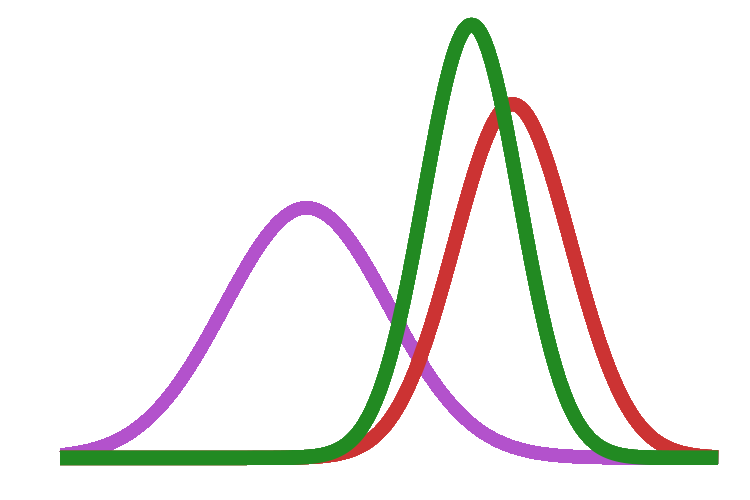
\includegraphics[width=0.9\textwidth]{turing.png}
		\end{column}
	\end{columns}
\end{frame}

\begin{frame}{\texttt{Turing.jl} Ecosystem}
	We have several Julia packages under \texttt{Turing.jl}'s GitHub
	organization \href{https://github.com/TuringLang}{TuringLang},
	but I will focus on 6 of those:

	\begin{vfilleditems}
		\small
		\item \href{https://github.com/TuringLang/Turing.jl}{\texttt{Turing.jl}}:
		main package that we use to \textbf{interface with all
			the Turing ecosystem} of packages and the backbone of
		everything
		\item \href{https://github.com/TuringLang/MCMCChains.jl}{\texttt{MCMCChains.jl}}:
		interface to \textbf{summarizing MCMC simulations} and
		has several utility functions for \textbf{diagnostics}
		and \textbf{visualizations}
		\item \href{https://github.com/TuringLang/DynamicPPL.jl}{\texttt{DynamicPPL.jl}}:
		specifies a domain-specific language for \texttt{Turing.jl},
		entirely written in Julia, and it is modular
		\item \href{https://github.com/TuringLang/AdvancedHMC.jl}{\texttt{AdvancedHMC.jl}}:
		modular and efficient implementation of advanced
		Hamiltonian Monte Carlo (HMC) algorithms
		\item \href{https://github.com/TuringLang/DistributionsAD.jl}{\texttt{DistributionsAD.jl}}:
		defines the necessary functions to enable automatic
		differentiation (AD) of the log PDF functions from
		\href{https://github.com/JuliaStats/Distributions.jl}{\texttt{Distributions.jl}}
		\item \href{https://github.com/TuringLang/Bijectors.jl}{\texttt{Bijectors.jl}}:
		implements a set of functions for transforming constrained
		random variables (\textit{e.g.} simplexes, intervals)
		to Euclidean space
	\end{vfilleditems}
\end{frame}

\begin{frame}[fragile]{\texttt{Turing.jl}\footnote{
			I believe in Julia's potential and wrote a whole set of
			\href{https://storopoli.github.io/Bayesian-Julia}{
				Bayesian Statistics tutorials using Julia and
				\texttt{Turing.jl}} \parencite{storopoli2021bayesianjulia}}
		Code Example}
	\begin{lstlisting}[basicstyle=\small, language=Matlab, escapeinside=\{\}]
        @model linreg({$x_1$}, {$x_2$}, y) = begin
            {$\alpha$} ~ Normal(0, 20)
            {$\beta_1$} ~ Normal(0, 2)
            {$\beta_2$} ~ Normal(0, 2)
            {$\sigma$} ~ truncated(Cauchy(0, 2.5); lower=0)

            y .~ Normal({$\alpha$} .+ {$\beta_1$} * {$x_1$} + {$\beta_2$} * {$x_2$}, {$\sigma$})
        end
    \end{lstlisting}
\end{frame}

\begin{frame}{\texttt{Stan} and \texttt{Julia} mentioned in Billions\footnote{
			If you cannot watch the video \href{https://github.com/storopoli/Bayesian-Statistics/blob/main/slides/images/stan_billions_subtitled.mp4?raw=true}{click here}
			to see it in your browser.} (Season 3 Episode 9)}
	\centering
	\includemedia[
		width=\linewidth,
		height=0.3\linewidth,
		addresource=stan_billions_subtitled.mp4,
		transparent,
		activate=pageopen,
		passcontext,  %show VPlayer's right-click menu
		flashvars={
				source=stan_billions_subtitled.mp4
				&loop=true
				&scaleMode=stretch
			}
	]{\texttt{Stan} and Julia mentioned in Billions}{http://mirrors.ctan.org/macros/latex/contrib/media9/players/VPlayer.swf}
\end{frame}

\subsection{PyMC}
\begin{frame}{\texttt{PyMC}\footnote{\textcite{pymc3}}}
	\begin{columns}
		\begin{column}{0.8\textwidth}
			\begin{vfilleditems}
				\small
				\item Python package for Bayesian statistics
				with a Markov Chain Monte Carlo sampler
				\item Financial support from \href{https://numfocus.org/}{NUMFocus}
				\item Backend was based on \texttt{Theano}
				\item \texttt{Theano} \textbf{died}, but \texttt{PyMC} developers create a fork
				named \texttt{Aesara}
				\item We have no idea what will be the backend in
				the future.
				\texttt{PyMC} developers are still experimenting with other
				backends: \texttt{TensorFlow Probability}, \texttt{NumPyro}
				and so on ...
			\end{vfilleditems}
		\end{column}
		\begin{column}{0.2\textwidth}
			\centering
			
\includegraphics[width=0.9\textwidth]{pymc.png}
		\end{column}
	\end{columns}
\end{frame}

\begin{frame}[fragile]{\texttt{PyMC} Code Example}
	\begin{lstlisting}[basicstyle=\small, language=Python]
    with pm.Model() as model:
        alpha = pm.Normal("Intercept", mu=0, sigma=20)
        beta_1 = pm.Normal("beta_1", mu=0, sigma=2)
        beta_2 = pm.Normal("beta_2", mu=0, sigma=2)
        sigma = pm.HalfCauchy("sigma", beta=2.5)

        likelihood = pm.Normal("y",
                     mu=alpha + beta_1 * x1 + beta_2 * x2,
                     sigma=sigma, observed=y)
\end{lstlisting}
\end{frame}

\subsection{Which Tool You Should Use?}
\begin{frame}{Which Tool You Should Use?}
	\begin{columns}
		\begin{column}{0.5\textwidth}
			\centering
			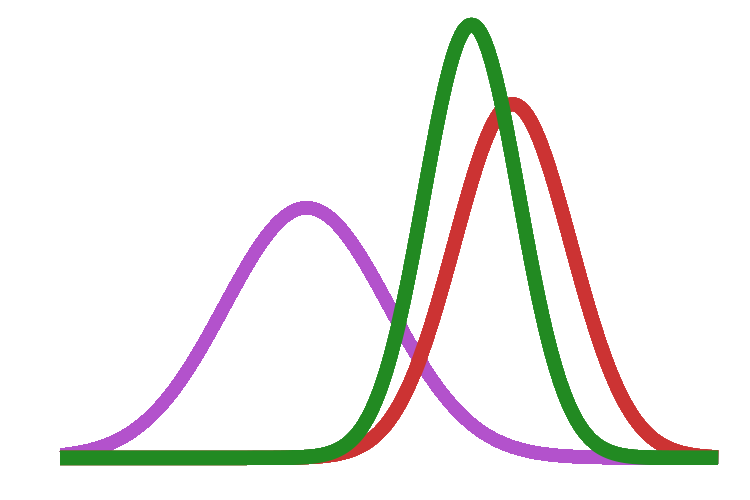
\includegraphics[width=0.9\textwidth]{turing.png}
		\end{column}
		\begin{column}{0.5\textwidth}
			\centering
			
\includegraphics[width=0.7\textwidth]{stan.png}
		\end{column}
	\end{columns}
\end{frame}

\begin{frame}{Why \texttt{Turing.jl}}
	\begin{vfilleditems}
		\item \textbf{Julia} all the way down...
		\item Can \textbf{interface/compose} with \textit{any} Julia package.
		\item Decoupling of \textbf{modeling DSL, inference algorithms and data}.
		\item Not only HMC-NUTS, but a whole \textbf{plethora of MCMC algorithms}, e.g. Metropolis-Hastings, Gibbs, SMC, IS etc.
		\item Easy to \textbf{create/prototype/modify inference algorithms}.
		\item \textbf{Transparent MCMC workflow}, e.g. iterative sampling API allows step-wise execution and debugging of the inference algorithm
		\item Very easy to \textbf{do stuff in the GPU}, e.g. NVIDIA's \texttt{CUDA.jl}, AMD's \texttt{AMDGPU.jl}, and Intel's \texttt{oneAPI.jl}.
		\item Very easy to do \textbf{distributed model inference and prediction}.
	\end{vfilleditems}
\end{frame}

\begin{frame}{Why \textit{not} \texttt{Turing}}
	\begin{vfilleditems}
		\item \textbf{Not as fast}, but pretty close behind, as \texttt{Stan}.
		\item \textbf{Not enough learning materials}, example models, tutorials.
		Also documentation is somewhat lacking in certain areas, e.g. \texttt{Bijectors.jl}.
		\item \textbf{Not as many citations as \texttt{Stan}},
		although not very far behind in GitHub stars.
		\item \textbf{Not well-known in the academic community}.
	\end{vfilleditems}
\end{frame}

\begin{frame}{Why \texttt{Stan}}
	\begin{vfilleditems}
		\item API for R, Python and Julia.
		\item Faster than \texttt{Turing.jl} in 95\% of models.
		\item \textbf{Well-known in the academic community}.
		\item \textbf{High citation count}.
		\item \textbf{More tutorials, example models, and learning materials available}.
	\end{vfilleditems}
\end{frame}

\begin{frame}{Why \textit{not} \texttt{Stan}}
	\begin{vfilleditems}
		\item If you want to try \textbf{something new}, you'll have to do in \textbf{C++}.
		\item Constrained \textbf{only to HMC-NUTS} as MCMC algorithm.
		\item \textbf{Cannot decouple model DSL from data} (and also from inference algorithm).
		\item \textbf{Does not compose well with other packages}.
		For anything you want to do, it has to ``exist'' in the \texttt{Stan} world,
		e.g. \texttt{bayesplot}.
		\item A \textbf{not so easy and intuitive ODE interface}.
		\item \textbf{GPU interface depends on OpenCL}.
		Also not easy to interoperate.
	\end{vfilleditems}
\end{frame}

\section{Bayesian Statistics}

\subsection{Recommended References}
\begin{frame}{Bayesian Statistics - Recommended References}
	\begin{vfilleditems}
		\item \textcite{gelman2013bayesian} - Chapter 1: Probability and inference
		\item \textcite{mcelreath2020statistical} - Chapter 1: The Golem of Prague
		\item \textcite{gelman2020regression} - Chapter 3: Some basic methods in mathematics and probability
		\item \textcite{khanBayesianLearningRule2021}
		\item \textbf{Probability}:
		\begin{vfilleditems}
			\item A great textbook - \textcite{bertsekasIntroductionProbability2nd2008}
			\item Also a great textbook (skip the frequentist part)- \textcite{dekkingModernIntroductionProbability2010}
			\item Bayesian point-of-view and also a philosophical approach- \textcite{jaynesProbabilityTheoryLogic2003}
			\item Bayesian point-of-view with a simple and playful approach - \textcite{kurtBayesianStatisticsFun2019}
			\item Philosophical approach not so focused on mathematical rigor - \textcite{diaconisTenGreatIdeas2019}
		\end{vfilleditems}
	\end{vfilleditems}
\end{frame}

\subsection{What is Bayesian Statistics?}
\begin{frame}{What is Bayesian Statistics?}
	Bayesian statistics is a \textbf{data analysis approach based on Bayes' theorem}
	where available knowledge about the parameters of a statistical model
	is updated with the information of observed data.
	\parencite{gelman2013bayesian}.
	Previous knowledge is expressed as a \textbf{prior} distribution
	and combined with the observed data in the form of a \textbf{likelihood} function
	to generate a \textbf{posterior} distribution.
	The posterior can also be used to make predictions about future events.
\end{frame}

\subsubsection{What changes from Frequentist Statistics?}
\begin{frame}{What changes from Frequentist Statistics?}
	\begin{vfilleditems}
		\item \textbf{Flexibility} - probabilistic building blocks to
		construct a model\footnote{like LEGO}:
		\begin{vfilleditems}
			\item Probabilistic conjectures about parameters:
			\begin{vfilleditems}
				\item Prior
				\item Likelihood
			\end{vfilleditems}
		\end{vfilleditems}
		\item Better \textbf{uncertainty} treatment:
		\begin{vfilleditems}
			\item Coherence
			\item Propagation
			\item We don't use \textit{``if we sampled infinite times
				from a population that we do not observe...''}
		\end{vfilleditems}
		\item No \textbf{$p$-values}:
		\begin{vfilleditems}
			\item All statistical intuitions makes \textbf{sense}
			\item 95\% certainty that $\theta$'s parameter value is
			between $x$ and $y$
			\item Almost \textbf{impossible} to perform $p$-hacking
		\end{vfilleditems}
	\end{vfilleditems}
\end{frame}

\begin{frame}{A little bit more formal}
	\begin{vfilleditems}
		\item Bayesian Statistics uses probabilistic statements:
		\begin{vfilleditems}
			\item one or more parameters $\theta$
			\item unobserved data $\tilde{y}$
		\end{vfilleditems}
		\item These statements are conditioned on the observerd values of $y$:
		\begin{vfilleditems}
			\item $P(\theta \mid y)$
			\item $P(\tilde{y} \mid y)$
		\end{vfilleditems}
		\item We also, implicitly, conditioned on the observed data from
		any covariate $x$
	\end{vfilleditems}
\end{frame}

\begin{frame}{Definition of Bayesian Statistics}
	\begin{defn}[Bayesian Statistics]
		The use of Bayes theorem as the procedure to \textbf{estimate
			parameters of interest $\theta$ or unobserved data $\tilde{y}$}.
		\parencite{gelman2013bayesian}
	\end{defn}
\end{frame}

\subsection{Tools}
\begin{frame}{Tools}
	\centering
	\textit{``A man and his tools make a man and his trade''}

	\vspace{2ex}

	Vita Sackville-West
\end{frame}

\begin{frame}{Tools}
	\begin{vfilleditems}
		\item \LARGE  \href{https://mc-stan.org}{\texttt{Stan}} (BSD-3 License)
		\item \LARGE  \href{https://turing.ml}{\texttt{Turing.jl}} (MIT License)
		\item \href{https://www.pymc.io/}{\texttt{PyMC}} (Apache License)
		\item \small \href{https://mcmc-jags.sourceforge.io/}{\texttt{JAGS}} (GPL License)
		\item \footnotesize \href{https://www.mrc-bsu.cam.ac.uk/software/bugs/}{\texttt{BUGS}} (GPL License)
	\end{vfilleditems}
\end{frame}

\subsubsection{Stan}
\begin{frame}{\texttt{Stan}\footnote{\textcite{carpenterStanProbabilisticProgramming2017}}}
	\begin{columns}
		\begin{column}{0.8\textwidth}
			\begin{vfilleditems}
				\small
				\item High-performance platform for statistical
				modeling and  statistical computation
				\item Financial support from
				\href{https://numfocus.org/}{NUMFocus}:
				\begin{vfilleditems}
					\footnotesize
					\item AWS Amazon
					\item Bloomberg
					\item Microsoft
					\item IBM
					\item RStudio
					\item Facebook
					\item NVIDIA
					\item Netflix
				\end{vfilleditems}
				\small
				\item Open-source language, similar to \texttt{C++}
				\item Markov Chain Monte Carlo (MCMC) parallel sampler
			\end{vfilleditems}
		\end{column}
		\begin{column}{0.2\textwidth}
			\centering
			
\includegraphics[width=0.9\textwidth]{stan.png}
		\end{column}
	\end{columns}
\end{frame}

\begin{frame}[fragile]{\texttt{Stan} Code Example}
	\begin{lstlisting}[basicstyle=\footnotesize, language=Stan]
        data {
          int<lower=0> N;
          vector[N] x1;
          vector[N] x2;
          vector[N] y;
        }
        parameters {
          real alpha;
          real beta1;
          real beta2;
          real<lower=0> sigma;
        }
        model {
          alpha ~ normal(0, 20);
          beta1 ~ normal(0, 2);
          beta2 ~ normal(0, 2);
          sigma ~ cauchy(0, 2.5);
          y ~ normal(alpha + beta1 * x1 + beta2 * x2, sigma);
        }
    \end{lstlisting}
\end{frame}

\subsubsection{Turing.jl}
\begin{frame}{\texttt{Turing.jl}\footnote{\textcite{geTuringLanguageFlexible2018}}}
	\begin{columns}
		\begin{column}{0.8\textwidth}
			\begin{vfilleditems}
				\small
				\item Ecosystem of Julia packages for Bayesian
				Inference using probabilistic programming
				\item \href{https://www.julialang.org}{Julia} is a fast
				dynamic-typed language that just-in-time (JIT)
				compiles into native code using LLVM:
				\href{https://www.nature.com/articles/d41586-019-02310-3}{``runs like C but reads like Python''};
				meaning that is \textit{blazing} fast, easy to prototype and read/write code
				\item Julia has Financial support from
				\href{https://numfocus.org/}{NUMFocus}
				\item Composability with other Julia packages
				\item Several other options of Markov Chain Monte Carlo (MCMC) samplers
			\end{vfilleditems}
		\end{column}
		\begin{column}{0.2\textwidth}
			\centering
			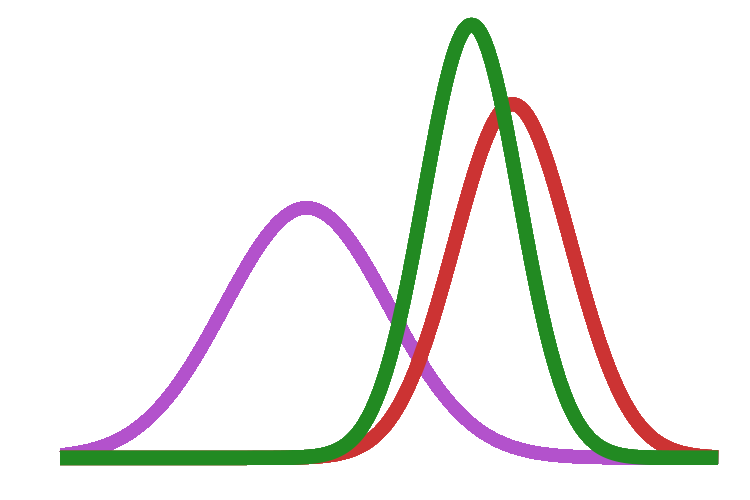
\includegraphics[width=0.9\textwidth]{turing.png}
		\end{column}
	\end{columns}
\end{frame}

\begin{frame}{\texttt{Turing.jl} Ecosystem}
	We have several Julia packages under \texttt{Turing.jl}'s GitHub
	organization \href{https://github.com/TuringLang}{TuringLang},
	but I will focus on 6 of those:

	\begin{vfilleditems}
		\small
		\item \href{https://github.com/TuringLang/Turing.jl}{\texttt{Turing.jl}}:
		main package that we use to \textbf{interface with all
			the Turing ecosystem} of packages and the backbone of
		everything
		\item \href{https://github.com/TuringLang/MCMCChains.jl}{\texttt{MCMCChains.jl}}:
		interface to \textbf{summarizing MCMC simulations} and
		has several utility functions for \textbf{diagnostics}
		and \textbf{visualizations}
		\item \href{https://github.com/TuringLang/DynamicPPL.jl}{\texttt{DynamicPPL.jl}}:
		specifies a domain-specific language for \texttt{Turing.jl},
		entirely written in Julia, and it is modular
		\item \href{https://github.com/TuringLang/AdvancedHMC.jl}{\texttt{AdvancedHMC.jl}}:
		modular and efficient implementation of advanced
		Hamiltonian Monte Carlo (HMC) algorithms
		\item \href{https://github.com/TuringLang/DistributionsAD.jl}{\texttt{DistributionsAD.jl}}:
		defines the necessary functions to enable automatic
		differentiation (AD) of the log PDF functions from
		\href{https://github.com/JuliaStats/Distributions.jl}{\texttt{Distributions.jl}}
		\item \href{https://github.com/TuringLang/Bijectors.jl}{\texttt{Bijectors.jl}}:
		implements a set of functions for transforming constrained
		random variables (\textit{e.g.} simplexes, intervals)
		to Euclidean space
	\end{vfilleditems}
\end{frame}

\begin{frame}[fragile]{\texttt{Turing.jl}\footnote{
			I believe in Julia's potential and wrote a whole set of
			\href{https://storopoli.io/Bayesian-Julia}{
				Bayesian Statistics tutorials using Julia and
				\texttt{Turing.jl}} \parencite{storopoli2021bayesianjulia}}
		Code Example}
	\begin{lstlisting}[basicstyle=\small, language=Matlab, escapeinside=\{\}]
        @model linreg({$x_1$}, {$x_2$}, y) = begin
            {$\alpha$} ~ Normal(0, 20)
            {$\beta_1$} ~ Normal(0, 2)
            {$\beta_2$} ~ Normal(0, 2)
            {$\sigma$} ~ truncated(Cauchy(0, 2.5); lower=0)

            y .~ Normal({$\alpha$} .+ {$\beta_1$} * {$x_1$} + {$\beta_2$} * {$x_2$}, {$\sigma$})
        end
    \end{lstlisting}
\end{frame}

\begin{frame}{\texttt{Stan} and \texttt{Julia} mentioned in Billions\footnote{
			If you cannot watch the video \href{https://github.com/storopoli/Bayesian-Statistics/blob/main/images/stan_billions_subtitled.mp4?raw=true}{click here}
			to see it in your browser.} (Season 3 Episode 9)}
	\centering
	\includemedia[
		width=\linewidth,
		height=0.3\linewidth,
		addresource=stan_billions_subtitled.mp4,
		transparent,
		activate=pageopen,
		passcontext,  %show VPlayer's right-click menu
		flashvars={
				source=stan_billions_subtitled.mp4
				&loop=true
				&scaleMode=stretch
			}
	]{\texttt{Stan} and Julia mentioned in Billions}{http://mirrors.ctan.org/macros/latex/contrib/media9/players/VPlayer.swf}
\end{frame}

\subsubsection{PyMC}
\begin{frame}{\texttt{PyMC}\footnote{\textcite{pymc3}}}
	\begin{columns}
		\begin{column}{0.8\textwidth}
			\begin{vfilleditems}
				\small
				\item Python package for Bayesian statistics
				with a Markov Chain Monte Carlo sampler
				\item Financial support from \href{https://numfocus.org/}{NUMFocus}
				\item Backend was based on \texttt{Theano}
				\item \texttt{Theano} \textbf{died}, but \texttt{PyMC} developers create a fork
				named \texttt{Aesara}
				\item We have no idea what will be the backend in
				the future.
				\texttt{PyMC} developers are still experimenting with other
				backends: \texttt{TensorFlow Probability}, \texttt{NumPyro}
				and so on ...
			\end{vfilleditems}
		\end{column}
		\begin{column}{0.2\textwidth}
			\centering
			
\includegraphics[width=0.9\textwidth]{pymc.png}
		\end{column}
	\end{columns}
\end{frame}

\begin{frame}[fragile]{\texttt{PyMC} Code Example}
	\begin{lstlisting}[basicstyle=\small, language=Python]
    with pm.Model() as model:
        alpha = pm.Normal("Intercept", mu=0, sigma=20)
        beta_1 = pm.Normal("beta_1", mu=0, sigma=2)
        beta_2 = pm.Normal("beta_2", mu=0, sigma=2)
        sigma = pm.HalfCauchy("sigma", beta=2.5)

        likelihood = pm.Normal("y",
                     mu=alpha + beta_1 * x1 + beta_2 * x2,
                     sigma=sigma, observed=y)
\end{lstlisting}
\end{frame}

\subsection{Probability}
\begin{frame}{PROBABILITY DOES NOT EXIST!\footnote{\textcite{definettiTheoryProbability1974}}}
	\begin{columns}
		\begin{column}{0.8\textwidth}
			\begin{vfilleditems}
				\item Yes, probability does not exist ...
				\item Or even better, probability as a physical quantity,
				objective chance, \textbf{does NOT exist}
				\item if we disregard objetive chance \textit{nothing is lost}
				\item The math of inductive rationality remains
				\textbf{exactly the same}
			\end{vfilleditems}
		\end{column}
		\begin{column}{0.2\textwidth}
			\centering
			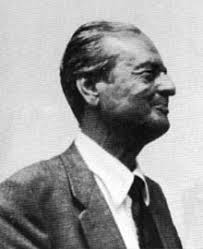
\includegraphics[width=0.9\columnwidth]{finetti.jpg}
		\end{column}
	\end{columns}
\end{frame}

\begin{frame}{PROBABILITY DOES NOT EXIST!\footnote{\textcite{definettiTheoryProbability1974}}}
	\begin{columns}
		\begin{column}{0.6\textwidth}
			\begin{vfilleditems}
				\small
				\item Consider flipping a biased coin
				\item The trials are considered independent and, as a result,
				have an important property: \textbf{the order does not matter}
				\item The frequency is considered a \textbf{sufficient statistic}
				\item Saying that order does not matter or saying that the only thing that
				matters is frequency are two ways of saying the same thing
				\item We say that the probability is \textbf{invariant under permutations}
			\end{vfilleditems}
		\end{column}
		\begin{column}{0.4\textwidth}
			\begin{tikzpicture}[
					scale=0.55,
					transform shape, thick,
					every node/.style = {draw, circle, minimum size = 10mm},
					grow = down,  % alignment of characters
					level 1/.style = {sibling distance=3cm},
					level 2/.style = {sibling distance=1.5cm},
					level 3/.style = {sibling distance=3cm},
					level distance = 3cm,
					head/.style = {fill = orange!90!blue,
							label = center:\textsf{\Large H}},
					tail/.style = {fill = blue!70!yellow, text = black,
							label = center:\textsf{\Large T}}
				]
				\node[shape = circle split, draw, line width = 1pt,
					minimum size = 10mm, inner sep = 0mm, font = \sffamily\large,
					rotate=30] (Start)
				{ \rotatebox{-30}{H} \nodepart{lower} \rotatebox{-30}{T}}
				child {   node [head] (A) {}
						child { node [head] (B) {}}
						child { node [tail] (C) {}}
					}
				child {   node [tail] (D) {}
						child { node [head] (E) {}}
						child { node [tail] (F) {}}
					};

				% Filling the root (Start)
				\begin{scope}[on background layer, rotate=30]
					\fill[head] (Start.base) ([xshift = 0mm]Start.east) arc (0:180:5mm)
					-- cycle;
					\fill[tail] (Start.base) ([xshift = 0pt]Start.west) arc (180:360:5mm)
					-- cycle;
				\end{scope}

				% Labels
				\begin{scope}[nodes = {draw = none}]
					\path (Start) -- (A) node [near start, left]  {$0.5$};
					\path (A)     -- (B) node [near start, left]  {$0.5$};
					\path (A)     -- (C) node [near start, right] {$0.5$};
					\path (Start) -- (D) node [near start, right] {$0.5$};
					\path (D)     -- (E) node [near start, left]  {$0.5$};
					\path (D)     -- (F) node [near start, right] {$0.5$};
					\begin{scope}[nodes = {below = 11pt}]
						\node at (B) {$0.25$};
						\node at (C) {$0.25$};
						\node at (E) {$0.25$};
						\node at (F) {$0.25$};
					\end{scope}
				\end{scope}
			\end{tikzpicture}
		\end{column}
	\end{columns}
\end{frame}

\begin{frame}{Probability Interpretations}
	\begin{vfilleditems}
		\item \textbf{Objective} - frequency in the long run for an event:
		\begin{vfilleditems}
			\item $P(\text{rain}) = \frac{\text{days that rained}}{\text{total days}}$
			\item $P(\text{me being elected president}) = 0$ (never occurred)
		\end{vfilleditems}
		\item \textbf{Subjective} - degrees of belief in an event:
		\begin{vfilleditems}
			\item $P(\text{rain}) = \text{degree of belief that will rain}$
			\item $P(\text{me being elected president}) = 10^{-10}$ (highly unlikely)
		\end{vfilleditems}
	\end{vfilleditems}
\end{frame}

\subsubsection{What is Probability?}
\begin{frame}{What is Probability?}
	\begin{defn}[Probability]
		We define $A$ is an event and $P(A)$ the probability of event $A$.
		$P(A)$ has to be between $0$ and $1$, where higher values defines
		higher probability of $A$ happening.
		$$\begin{aligned}
				P(A)   & \in \mathbb{R} \\
				P(A)   & \in [0,1]      \\
				0 \leq & P(A) \leq 1
			\end{aligned}$$
	\end{defn}
\end{frame}

\begin{frame}{Probability Axioms\footnote{\textcite{kolmogorovFoundationsTheoryProbability1933}}}
	\begin{columns}
		\begin{column}{0.8\textwidth}
			\begin{vfilleditems}
				\item \textbf{Non-negativity}: For every $A$:
				$$P(A) \geq 0$$
				\item \textbf{Additivity}: For evey two \textit{mutually exclusive}
				$A$ and $B$:
				$$P(A) = 1 - P(B) \text{ and } P(B) = 1 - P(A)$$
				\item \textbf{Normalization}: The probability of all possible
				events $A_1, A_2, \dots$ must sum up to $1$:
				$$\sum_{n \in \mathbb{N}} A_n = 1$$
			\end{vfilleditems}
		\end{column}
		\begin{column}{0.2\textwidth}
			\centering
			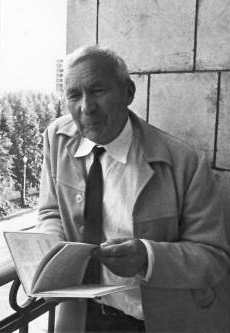
\includegraphics[width=0.9\columnwidth]{kolmogorov.jpg}
		\end{column}
	\end{columns}
\end{frame}

\begin{frame}{Sample Space}
	\begin{vfilleditems}
		\item Discrete $$\Theta = \left\{1, 2, \ldots \right\}$$
		\item Continuous $$\Theta \in \left(-\infty, \infty \right)$$
	\end{vfilleditems}
\end{frame}

\begin{frame}{Discrete Sample Space}
	8 planets in our solar system:
	\begin{vfilleditems}
		\item Mercury - $\mercury$
		\item Venus - $\venus$
		\item Earth - $\earth$
		\item Mars $\mars$
		\item Jupiter - $\jupiter$
		\item Saturn $\saturn$
		\item Uranus - $\uranus$
		\item Neptune $\neptune$
	\end{vfilleditems}
\end{frame}

\begin{frame}[fragile]{Discrete Sample Space\footnote{figure adapted from \href{https://github.com/betanalpha/stan_intro}{Michael Betancourt (CC-BY-SA-4.0)}}}
	\footnotesize
	\begin{figure}
		\centering
		\subfigure{
			\begin{tikzpicture}[scale=0.25, thick]
				\draw[color=black] (-25, 0) to (10, 0);
				\node[] at (-15, 0) {The planet has a magnetic field};
				\node[] at (7, 2) {$\theta \in E_{1}$};

				\fill[color=gray60] (0, 0) circle (25pt) node[color=black] {$\mercury$};
				\fill[color=blue] (2, 0) circle (25pt) node[color=black] {$\venus$};
				\fill[color=blue] (4, 0) circle (25pt) node[color=black] {$\earth$};
				\fill[color=gray60] (6, 0) circle (25pt) node[color=black] {$\mars$};
				\fill[color=blue] (8, 0) circle (25pt) node[color=black] {$\jupiter$};
				\fill[color=blue] (10, 0) circle (25pt) node[color=black] {$\saturn$};
				\fill[color=blue] (12, 0) circle (25pt) node[color=black] {$\uranus$};
				\fill[color=blue] (14, 0) circle (25pt) node[color=black] {$\neptune$};
			\end{tikzpicture}
		}
		%
		\subfigure{
			\begin{tikzpicture}[scale=0.25, thick]
				\draw[color=black] (-25, 0) to (10, 0);
				\node[] at (-15, 0) {The planet has moon(s)};
				\node[] at (7, 2) {$\theta \in E_{2}$};

				\fill[color=gray60] (0, 0) circle (25pt) node[color=black] {$\mercury$};
				\fill[color=gray60] (2, 0) circle (25pt) node[color=black] {$\venus$};
				\fill[color=blue] (4, 0) circle (25pt) node[color=black] {$\earth$};
				\fill[color=blue] (6, 0) circle (25pt) node[color=black] {$\mars$};
				\fill[color=blue] (8, 0) circle (25pt) node[color=black] {$\jupiter$};
				\fill[color=blue] (10, 0) circle (25pt) node[color=black] {$\saturn$};
				\fill[color=blue] (12, 0) circle (25pt) node[color=black] {$\uranus$};
				\fill[color=blue] (14, 0) circle (25pt) node[color=black] {$\neptune$};
			\end{tikzpicture}
		}
		%
		\subfigure{
			\begin{tikzpicture}[scale=0.25, thick]
				\draw[color=black] (-25, 0) to (10, 0);
				\node[] at (-15, 0) {The planet has a magnetic field \textit{and} moon(s)};
				\node[] at (7, 2) {$\theta \in E_{1} \cap E_{2}$};

				\fill[color=gray60] (0, 0) circle (25pt) node[color=black] {$\mercury$};
				\fill[color=gray60] (2, 0) circle (25pt) node[color=black] {$\venus$};
				\fill[color=blue] (4, 0) circle (25pt) node[color=black] {$\earth$};
				\fill[color=gray60] (6, 0) circle (25pt) node[color=black] {$\mars$};
				\fill[color=blue] (8, 0) circle (25pt) node[color=black] {$\jupiter$};
				\fill[color=blue] (10, 0) circle (25pt) node[color=black] {$\saturn$};
				\fill[color=blue] (12, 0) circle (25pt) node[color=black] {$\uranus$};
				\fill[color=blue] (14, 0) circle (25pt) node[color=black] {$\neptune$};
			\end{tikzpicture}
		}
		%
		\subfigure{
			\begin{tikzpicture}[scale=0.25, thick]
				\node[] at (-15, 0) {The planet has a magnetic field \textit{or} moon(s)};
				\node[] at (7, 2) {$\theta \in E_{1} \cup E_{2}$};

				\fill[color=gray60] (0, 0) circle (25pt) node[color=black] {$\mercury$};
				\fill[color=blue] (2, 0) circle (25pt) node[color=black] {$\venus$};
				\fill[color=blue] (4, 0) circle (25pt) node[color=black] {$\earth$};
				\fill[color=blue] (6, 0) circle (25pt) node[color=black] {$\mars$};
				\fill[color=blue] (8, 0) circle (25pt) node[color=black] {$\jupiter$};
				\fill[color=blue] (10, 0) circle (25pt) node[color=black] {$\saturn$};
				\fill[color=blue] (12, 0) circle (25pt) node[color=black] {$\uranus$};
				\fill[color=blue] (14, 0) circle (25pt) node[color=black] {$\neptune$};
			\end{tikzpicture}
		}
		%
		\subfigure{
			\begin{tikzpicture}[scale=0.25, thick]
				\node[] at (-15, 0) {The planet does \textit{not} have a magnetic field};
				\node[] at (7, 2) {$\theta \in \neg E_{1}$};

				\fill[color=blue] (0, 0) circle (25pt) node[color=black] {$\mercury$};
				\fill[color=gray60] (2, 0) circle (25pt) node[color=black] {$\venus$};
				\fill[color=gray60] (4, 0) circle (25pt) node[color=black] {$\earth$};
				\fill[color=blue] (6, 0) circle (25pt) node[color=black] {$\mars$};
				\fill[color=gray60] (8, 0) circle (25pt) node[color=black] {$\jupiter$};
				\fill[color=gray60] (10, 0) circle (25pt) node[color=black] {$\saturn$};
				\fill[color=gray60] (12, 0) circle (25pt) node[color=black] {$\uranus$};
				\fill[color=gray60] (14, 0) circle (25pt) node[color=black] {$\neptune$};
			\end{tikzpicture}
		}
		%
	\end{figure}
\end{frame}

\begin{frame}{Continuous Sample Space\footnote{
			figure adapted from \href{https://github.com/betanalpha/stan_intro}{Michael Betancourt (CC-BY-SA-4.0)}}
	}
	\footnotesize
	\begin{figure}
		\centering
		\subfigure{
			\begin{tikzpicture}[scale=0.25, thick]
				\draw[color=black] (-27, 0) to (17, 0);
				\node[align=center] at (-15, 0) {The distance is less than five centimeters};
				\node[] at (7.5, 2) {$\theta \in E_{1}$};

				\draw[|->] (0, 0) -- (14,0) node[right] {$x$};
				\draw[line width=1mm, color=blue] (0, 0) node[] {$\,($} -- (5, 0) node[] {$\!)$};
			\end{tikzpicture}
		}
		%
		\subfigure{
			\begin{tikzpicture}[scale=0.25, thick]
				\draw[color=black] (-27, 0) to (17, 0);
				\node[align=center] at (-15, 0) {The distance is between three and seven centimeters};
				\node[] at (7.5, 2) {$\theta \in E_{2}$};

				\draw[|->] (0, 0) -- (14,0) node[right] {$x$};
				\draw[line width=1mm, color=blue] (3, 0) node[] {$\,($} -- (7,0) node[] {$\!)$};

			\end{tikzpicture}
		}
		%
		\subfigure{
			\begin{tikzpicture}[scale=0.25, thick]
				\draw[color=black] (-27, 0) to (17, 0);
				\node[align=center] at (-15, 0) {The distance is less than five centimeters \\ \textit{and} e between three and seven centimeters};
				\node[] at (7.5, 2) {$\theta \in E_{1} \cap E_{2}$};

				\draw[|->] (0, 0) -- (14,0) node[right] {$x$};
				\draw[line width=1mm, color=blue] (3, 0) node[] {$\,($} -- (5, 0) node[] {$\!)$};
			\end{tikzpicture}
		}
		%
		\subfigure{
			\begin{tikzpicture}[scale=0.25, thick]
				\draw[color=black] (-27, 0) to (17, 0);
				\node[align=center] at (-15, 0) {The distance is less than five centimeters \\ \textit{or} between three and seven centimeters};
				\node[] at (7.5, 2) {$\theta \in E_{1} \cup E_{2}$};

				\draw[|->] (0, 0) -- (14, 0) node[right] {$x$};
				\draw[line width=1mm, color=blue] (0, 0) node[] {$\,($} -- (7, 0) node[] {$\!)$};
			\end{tikzpicture}
		}
		%		%
		\subfigure{
			\begin{tikzpicture}[scale=0.25, thick]
				\draw[color=black] (-27, 0) to (17, 0);
				\node[align=center] at (-15, 0) {The distance is \textit{not} less than five centimeters};
				\node[] at (7.5, 2) {$\theta \in \neg E_{1}$};

				\draw[|->] (0, 0) -- (14, 0) node[right] {$x$};
				\draw[line width=1mm, color=blue] (5, 0) node[] {$\,($} -- (13, 0);
			\end{tikzpicture}
		}
	\end{figure}
\end{frame}

\begin{frame}{Discrete versus Continuous Parameters}

	Everything that has been exposed here was under the assumption that the
	parameters are discrete.
	This was done with the intent to provide an intuition what is probability.
	Not always we work with discrete parameters.
	Parameters can be continuous, such as: age, height, weight etc.
	But don't despair!
	All probability rules and axioms are valid also for continuous parameters.
	The only thing we have to do is to change all sum $\sum$ for integrals $\int$.
	For example, the third axiom of \textbf{Normalization} for \textit{continuous}
	random variables becomes:
	$$
		\int_{x \in X} p(x) dx = 1.
	$$
\end{frame}


\begin{frame}{Conditional Probability}
	\begin{defn}[Conditional Probability]
		Probability of an event occurring in case another has occurred or not. \newline \newline
		The notation we use is $P( A \mid B )$, that read as ``the probability of
		observing $A$ given that we already observed $B$''. \newline \newline
		$$
			\begin{aligned}
				P(A \mid B) & = \frac{\text{number of elements in$A$ e $B$}}{\text{number of elements in $B$}} \\
				P(A \mid B) & = \frac{P(A \cap B)}{(B)}
			\end{aligned}
		$$
		\newline \hspace{0.7\textwidth}
		{\footnotesize assuming that $P(B) > 0$}.
	\end{defn}
\end{frame}

\begin{frame}{Example of Conditional Probability}
	\begin{example}[Poker Texas Hold'em]
		\begin{vfilleditems}
			\item \textbf{Sample Space}: $52$ cards in a deck, $13$ types of cards and $4$ types of suits.
			\item $P(A)$: Probability of being dealt an Ace $\left( \frac{4}{52} = \frac{1}{13}\right)$
			\item $P(K)$: Probability of being dealt a King $\left( \frac{4}{52} = \frac{1}{13} \right)$
			\item $P(A \mid K)$: Probability of being dealt an Ace, given that you have already a King $\left( \frac{4}{51} \approx 0.078 \right)$
			\item $P(K \mid A)$: Probability of being dealt a King, given that you have already an Ace $\left( \frac{4}{51} \approx 0.078 \right)$
		\end{vfilleditems}
	\end{example}
\end{frame}

\begin{frame}{Caution! Not always $P(A \mid B) = P(B \mid A)$}
	In the previous example we have the symmetry $P(A \mid K) = P(K \mid A)$,
	\textbf{but not always this is true}\footnote{
		More specific, if the basal rates $P(A)$ and $P(B)$ aren't equal,
		the symmetry is broken $P(A \mid B) \neq P(B \mid A)$}
	\begin{example}[The Pope is catholic]
		\begin{vfilleditems}
			\small{
				\item $P(\text{pope})$:
				Probability of some random person being the Pope,
				something really small, 1 in 8 billion $\left( \frac{1}{8 \cdot 10^9} \right)$
				\item $P(\text{catholic})$:
				Probability of some random person being catholic,
				1.34 billion in 8 billion $\left( \frac{1.34}{8} \approx 0.17 \right)$
				\item $P(\text{catholic} \mid \text{pope})$:
				Probability of the Pope being catholic $\left( \frac{999}{1000} = 0.999 \right)$
				\item $P(\text{pope} \mid \text{catholic})$:
				Probability of a catholic person being the Pope $\left( \frac{1}{1.34 \cdot 10^9} \cdot 0.999 \approx 7.46 \cdot 10^{-10} \right)$
			}
			\item \large{\textbf{Hence}: $P(\text{catholic} \mid \text{pope}) \neq P(\text{pope} \mid \text{catholic})$}
		\end{vfilleditems}
	\end{example}
\end{frame}

\begin{frame}{A Probability Textbook Classic}
	\begin{columns}
		\begin{column}{0.6\textwidth}
			\begin{example}[Monty Hall]
				\begin{vfilleditems}
					\small
					\item A TV presenter shows you 3 doors
					\item One of them has a prize: a car!
					The others have a goat
					\item You must choose a door (that is not open or revealed)
					\item In this moment, the presenter opens one of the other two doors
					that you did not choose,
					revealing one of the two goats
					\item The presenter then asks you
					``Do you want to change your door or stay with your choice?''
				\end{vfilleditems}
			\end{example}
		\end{column}
		\begin{column}{0.4\textwidth}
			\begin{figure}
				\centering
				\def\svgwidth{\columnwidth}
				\input{../images/monty_hall.pdf_tex}
			\end{figure}
		\end{column}
	\end{columns}
\end{frame}

\begin{frame}{Solution for the Monty Hall Problem}
	\begin{idea}[Probability of winning a car]
		$$
			\begin{aligned}
				P(\text{car} \mid C_i) & = \frac{1}{3}                                                                                                                    \\
				P(\text{car})          & = \frac{1}{3} \cdot P(\text{car} \mid C_1) + \frac{1}{3} \cdot P(\text{car} \mid C_2) + \frac{1}{3} \cdot P(\text{car} \mid C_3) \\
				P(\text{car})          & = \frac{\sum^3_{i=1}P(\text{car} \mid C_i)}{3}                                                                                   \\
				P(\text{car})          & = \frac{1}{3}
			\end{aligned}
		$$
	\end{idea}
	\vfill \vfill
	$C_i$ is the event that the car is behind door $i$, $i=1,2,3$
\end{frame}

\begin{frame}[t]{Solution for the Monty Hall Problem}
	\begin{columns}[t]
		\begin{column}{0.5\textwidth}
			{\Large \textbf{Scenario 1}: Don't change doors} \newline \newline
			Simple: $$\frac{1}{3}$$
		\end{column}
		\begin{column}{0.5\textwidth}
			{\Large \textbf{Scenario 2}: Change doors} \newline \newline
			Choose any door $i$ to be $C_i = 0$
			\vfill
			$$
				\begin{aligned}
					P(\text{car}) & = 0 \cdot P(\text{car} \mid C_i) + \frac{1}{3} + \frac{1}{3} \\
					P(\text{car}) & = \frac{2}{3}
				\end{aligned}
			$$
		\end{column}
	\end{columns}
\end{frame}

\begin{frame}{Visualization of the Monty Hall Problem}
	\begin{figure}
		\centering
		\subfigure{
			\begin{tikzpicture}[
					scale=0.55,
					header/.style = {draw, rectangle, fill = blue!50!black, minimum size = 10mm},
					level distance = 3.5cm,
					transform shape, thick,
					grow = right, sloped,
				]
				\node[header] {Your Choice}
				child{
						node[header] {Car is}
						edge from parent[draw=none]
						child{
								node[header] {Monty opens}
								edge from parent[draw=none]
								child{
										node[header] {result}
										edge from parent[draw=none]
									}
							}
					};
			\end{tikzpicture}
		}
		%
		\subfigure{
			\begin{tikzpicture}[
					scale=0.55,
					door/.style = {draw, circle, minimum size = 10mm},
					car/.style = {circle, fill = green!50!black, minimum size = 10mm},
					goat/.style = {circle, fill = red!50!black, minimum size = 10mm},
					level distance = 3.5cm,
					transform shape, thick,
					grow = right, sloped,
					level 1/.style = {sibling distance=3.5cm},
					level 2/.style = {sibling distance=2cm},
					level 3/.style = {sibling distance=3cm}
				]
				\node[door] {Door 1}
				child {
				node[door] {Door 3}
				child {
				node[door] {Door 2}
				child {
				node[car, label=right:{\Large$\frac{1}{3}$}] {Car}
				}
				edge from parent
				node[above] {\Large$1$}
				}
				edge from parent
				node[below] {\Large$\frac{1}{3}$}
				}
				child {
				node[door] {Door 2}
				child {
				node[door] {Door 3}
				child {
				node[car, label=right:{\Large$\frac{1}{3}$}] {Car}
				}
				edge from parent
				node[above] {\Large$1$}
				}
				edge from parent
				node[above] {\Large$\frac{1}{3}$}
				}
				child {
				node[door] {Door 1}
				child {
				node[door] {Door 2}
				child {
				node[goat, label=right:{\Large$\frac{1}{6}$}] {Goat}
				}
				edge from parent
				node[above]  {\Large$\frac{1}{2}$}
				}
				child {
				node[door] {Door 3}
				child {
				node[goat, label=right:{\Large$\frac{1}{6}$}] {Goat}
				}
				edge from parent
				node[above]  {\Large$\frac{1}{2}$}
				}
				edge from parent
				node[above] {\Large$\frac{1}{3}$}
				};
			\end{tikzpicture}
		}
	\end{figure}
\end{frame}

\begin{frame}{Joint Probability}
	\begin{defn}[Joint Probability]
		Probability of two or more events occurring. \newline \newline
		The notation we use is $P(A, B)$, that read as
		``the probability of observing $A$ and also observing $B$''. \newline \newline
		$$
			\begin{aligned}
				P(A,B) & = \text{number of elements in $A$ or $B$} \\
				P(A,B) & = P(A \cup B)                             \\
				P(A,B) & = P(B,A)
			\end{aligned}
		$$
	\end{defn}
\end{frame}

\begin{frame}{Example of Joint Probability}
	\begin{example}[Revisiting Poker Texas Hold'em]
		\begin{vfilleditems}
			{\footnotesize
				\item \textbf{Sample Space}: $52$ cards in a deck, $13$ types of cards and $4$ types of suits.
				\item $P(A)$: Probability of being dealt an Ace $\left( \frac{4}{52} = \frac{1}{13}\right)$
				\item $P(K)$: Probability of being dealt a King $\left( \frac{4}{52} = \frac{1}{13} \right)$
				\item $P(A \mid K)$: Probability of being dealt an Ace, given that you have already a King $\left( \frac{4}{51} \approx 0.078 \right)$
				\item $P(K \mid A)$: Probability of being dealt a King, given that you have already an Ace $\left( \frac{4}{51} \approx 0.078 \right)$
			}
			\item $P(A, K)$: Probability of being dealt an Ace \textit{and} being dealt a King
			$$
				\begin{aligned}
					P(A, K)                         & = P(K, A)                         \\
					P(A) \cdot P(K \mid A)          & = P(K) \cdot P(A \mid K)          \\
					\frac{1}{13} \cdot \frac{4}{51} & = \frac{1}{13} \cdot \frac{4}{51} \\
					                                & \approx 0.006
				\end{aligned}
			$$
		\end{vfilleditems}
	\end{example}
\end{frame}

%% Bivariate Normal adapted from: https://github.com/walmes/Tikz/blob/master/src/bivariate-normal.pgf
\begin{frame}{Visualization of Joint Probability versus Conditional Probability}
	\centering
	\begin{tikzpicture}[scale=0.9]
		\begin{axis}[
				domain   = -3.5:3.5,
				domain y = -3.5:3.5,
				view = {-70}{20},
				title={$P(X,Y)$ versus $P(X \mid Y=-0.75)$},
				xlabel={$X$},
				ylabel={$Y$},
				% zlabel={$SSE(\beta_0, \beta_1)$},
				zmin = -0,
				%xticklabels=\empty,
				%yticklabels=\empty,
				zticklabels=\empty,
				xtick=\empty,
				ytick={-0.75},
				ztick=\empty,
				axis z line*=none,
				axis y line*=left,
				axis x line*= bottom]
			\addplot3 [
				domain = -3.5:3.5,
				samples = 50, samples y = 0,
				thick, smooth, color = red, fill = orange, opacity = 0.75]
			(x, -0.75, {conditionalbinormal(-0.75, 0, 1, 0, 1, 0.75)});

			\draw (-3.5, -0.75, 0) -- (3.5, -0.75, 0);

			\addplot3 [
				surf,
				domain = -3.5:3.5,
				samples = 50,
				opacity = 0.15,
				faceted color = colorB,
				colormap = {blueblack}{
						color = (colorB)
						color = (colorA!50!white)
						color = (colorA)}]
			{binormal(0, 1, 0, 1, 0.7)};
		\end{axis}
	\end{tikzpicture}
\end{frame}

%% Countour plot adapted from: https://tex.stackexchange.com/a/31713/200209
\begin{frame}{Visualization of Joint Probability versus Conditional Probability}
	\begin{columns}
		\begin{column}{0.5\textwidth}
			\centering
			\begin{tikzpicture}[scale=0.5]
				\begin{axis}[
						view={0}{90},
						axis equal,
						enlarge y limits=true,
						title={$P(X,Y)$},
						xlabel={$X$},
						ylabel={$Y$},
						xtick=\empty,
						ytick={-0.75}
					]

					\draw[red, line width=2pt] (-3.5, -0.75) -- (3.5, -0.75);

					\addplot3[contour gnuplot={labels=false},domain=-3.5:3.5,domain y=-3.5:3.5]
					{exp(-( x^2 + y^2)/3 )};

				\end{axis}
			\end{tikzpicture}
		\end{column}
		\begin{column}{0.5\textwidth}
			\centering
			\begin{tikzpicture}[scale=0.5]
				\begin{axis}[every axis plot, line width=2pt,
						title={$P(X \mid Y=-0.75)$},
						xlabel={$X$},
						ylabel={$Y$},
						xtick=\empty,
						ytick=\empty,
						domain=-3.5:3.5,samples=200,
						axis x line*=bottom,  % no box around the plot, only x and y axis
						axis y line*=left,    % the * suppresses the arrow tips
						enlarge x limits=true % extend the axes a bit
					]

					\addplot [red, fill = red, fill opacity = 0.5] {exp(-( x^2 + -0.75^2)/3 )};
				\end{axis}
			\end{tikzpicture}
		\end{column}
	\end{columns}
\end{frame}

\subsubsection{Bayes Theorem}
\begin{frame}{Who was Thomas Bayes?}
	\begin{columns}
		\begin{column}{0.8\textwidth}
			\begin{vfilleditems}
				\item \small \textbf{Thomas Bayes} (1701 - 1761) was a statistician, philosopher
				and Presbyterian minister who is known for formulating a specific
				case of the theorem that bears his name: Bayes' theorem.
				\item \small Bayes never published what would become his most famous
				accomplishment; his notes were edited and published posthumously by
				his friend \textbf{Richard Price}.
				\item \small The theorem official name is \textbf{Bayes-Price-Laplace},
				because \textbf{Bayes} was the first to discover,
				\textbf{Price} got his notes, transcribed into mathematical notation,
				and read to the Royal Society of London,
				and \textbf{Laplace} independently rediscovered the theorem without
				having previous contact in the end of the XVIII century in France
				while using probability for statistical inference with census
				data in the Napoleonic era.
			\end{vfilleditems}
		\end{column}
		\begin{column}{0.2\textwidth}
			\centering
			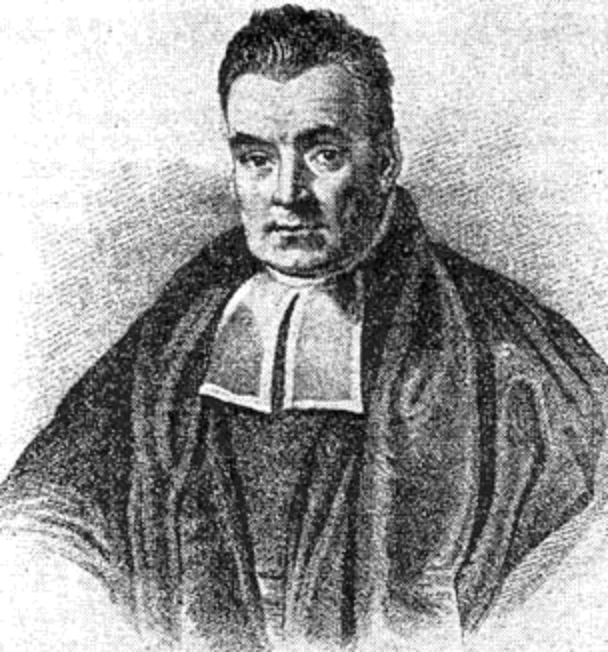
\includegraphics[width=0.9\columnwidth]{thomas_bayes.png}
		\end{column}
	\end{columns}
\end{frame}

\begin{frame}{Bayes Theorem}
	\begin{theorem}[Bayes]
		Tells us how to ``invert'' conditional probability: \newline \newline
		$$P(A \mid B) = \frac{P(A) \cdot P(B \mid A)}{P(B)}$$
	\end{theorem}
\end{frame}

\begin{frame}{Bayes' Theorem Proof}
	Remember the following probability identity:
	$$
		\begin{aligned}
			P(A,B)                 & = P(B,A)                 \\
			P(A) \cdot P(B \mid A) & = P(B) \cdot P(A \mid B)
		\end{aligned}
	$$

	OK, now divide everything by $P(B)$:
	$$
		\begin{aligned}
			\frac{P(A) \cdot P(B \mid A)}{P(B)} & = \frac{P(B) \cdot \quad P(A \mid B)}{P(B)} \\
			                                    &                                             \\
			\frac{P(A) \cdot P(B \mid A)}{P(B)} & = P(A \mid B)                               \\
			P(A \mid B)                         & = \frac{P(A) \cdot P(B \mid A)}{P(B)}
		\end{aligned}
	$$
\end{frame}

\begin{frame}{Another Probability Textbook Classic\footnote{Adapted from: \href{https://www.yudkowsky.net/rational/bayes}{Yudkowski - \textit{An Intuitive Explanation of Bayes’ Theorem}}.}}
	\begin{example}[Breast Cancer]
		\small
		How accurate is a \textbf{breast cancer} test?
		\begin{vfilleditems}
			\item \footnotesize 1\% of women have \textbf{breast cancer} (Prevalence)
			\item \footnotesize 80\% of mammograms detect \textbf{breast cancer} (True Positive)
			\item \footnotesize 9.6\% of mammograms detect \textbf{breast cancer} when there is no incidence (False Positive)
		\end{vfilleditems}
		$$
			\begin{aligned}
				P(C \mid +) & = \frac{P(+ \mid C) \cdot P(C)}{P(+)}                                                      \\
				P(C \mid +) & = \frac{P(+ \mid C) \cdot P(C)}{P(+ \mid C) \cdot P(C) + P(+ \mid \neg C) \cdot P(\neg C)} \\
				P(C \mid +) & = \frac{0.8 \cdot 0.01}{0.8 \cdot 0.01 + 0.096 \cdot 0.99}                                 \\
				P(C \mid +) & \approx 0.0776
			\end{aligned}
		$$
	\end{example}
\end{frame}


\begin{frame}{Why Bayes' Theorem is Important?}
	\begin{idea}[We can Invert the Conditional Probability]
		$$
			\begin{aligned}
				P(\text{hypothesis} \mid \text{data}) = \frac{P(\text{data} \mid \text{hypothesis}) \cdot P(\text{hypothesis})}{P(\text{data})}
			\end{aligned}
		$$
	\end{idea}
	But isn't this the $p$-value? \textcolor{red}{\textbf{NO!}}
\end{frame}

\subsection{Frequentist versus Bayesian}
\subsubsection{What are $p$-values and Confidence Intervals}
\begin{frame}{What are $p$-values?}
	\begin{defn}[$p$-value]
		$p$-value is the probability of obtaining results at least as
		extreme as the observed,
		given that the null hypothesis $H_0$ is true:
		$$P(D \mid H_0)$$
	\end{defn}
\end{frame}

\begin{frame}{What $p$-value is \textbf{not}!}
	\centering
	
\includegraphics[width=0.7\textwidth]{meme-pvalue.jpg}
\end{frame}

\begin{frame}{What $p$-value is \textbf{not}!}
	\begin{vfilleditems}
		\item \textbf{$p$-value is not the probability of the null hypothesis}
		- Infamous confusion between $P(D \mid H_0)$ and $P(H_0 \mid D)$.
		To get $P(H_0 \mid D)$ you need Bayesian statistics.
		\item \textbf{$p$-value is not the probability of data being generated at random}
		- \textcolor{red}{No!} We haven't stated nothing about randomness.
		\item \textbf{$p$-value measures the effect size of a statistical test}
		- Also \textcolor{red}{no}... $p$-value does not say anything about effect sizes.
		Just about if the observed data diverge of the expected under the null hypothesis.
		Besides, $p$-values can be hacked in several ways \parencite{head2015extent}.
	\end{vfilleditems}
\end{frame}

\begin{frame}{The relationship between $p$-value and $H_0$}
	To find out about any $p$-value, \textbf{find out what $H_0$ is behind it}.
	It's definition will never change, since it is always $P(D \mid H_0)$:
	\begin{vfilleditems}
		\item \textbf{$t$-test}: $P(D \mid \text{the difference between the groups is zero})$
		\item \textbf{ANOVA}: $P(D \mid \text{there is no difference between groups})$
		\item \textbf{Regression}: $P(D \mid \text{coefficient has a null value})$
		\item \textbf{Shapiro-Wilk}: $P(D \mid \text{population is distributed as a Normal distribution})$
	\end{vfilleditems}
\end{frame}

\begin{frame}{What are Confidence Intervals?}
	\begin{columns}
		\begin{column}{0.8\textwidth}
			\begin{defn}[Confidence Intervals]
				\begin{quotation}
					A confidence interval of X\% for a parameter is an interval
					$(a, b)$ generated by a repeated sampling procedure
					has probability X\% of containing the true value of the parameter,
					for all possible values of the parameter.
				\end{quotation}
				\vfill \vfill
				\textcite{neyman1937outline} (the ``father'' of confidence intervals)
			\end{defn}
		\end{column}
		\begin{column}{0.2\textwidth}
			\centering
			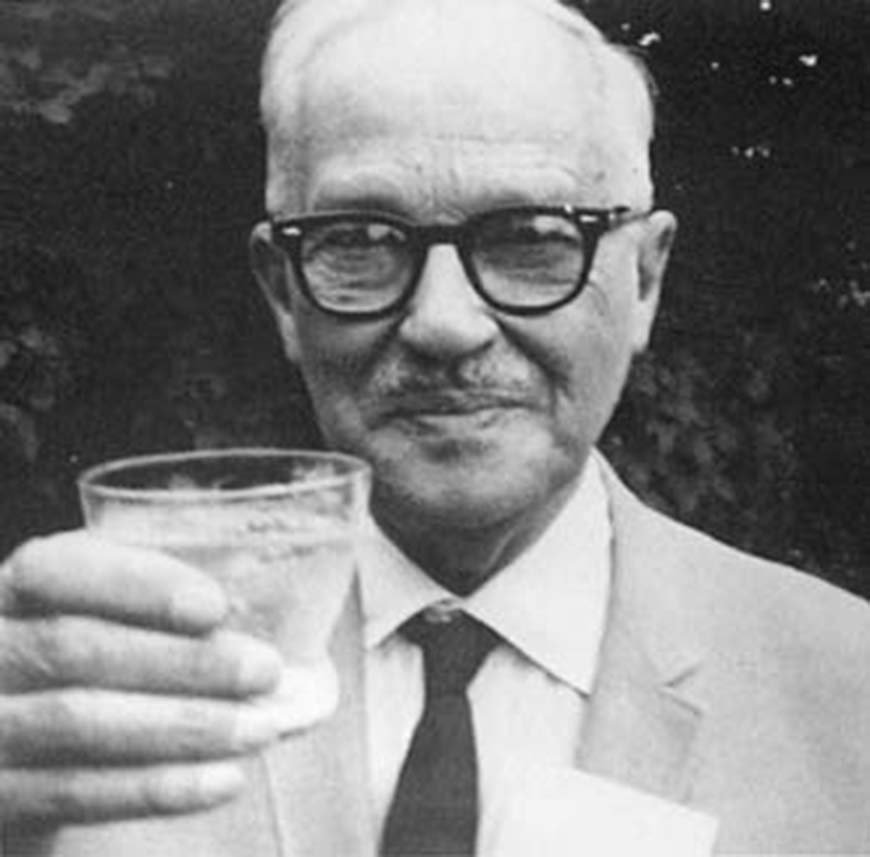
\includegraphics[width=0.9\columnwidth]{neyman.jpeg}
		\end{column}
	\end{columns}
\end{frame}

\begin{frame}{What are Confidence Intervals?}
	\begin{example}[Confidence Intervals of a Public Policy Analysis]
		Say you performed a statistical analysis to compare
		the efficacy of a public policy between two groups and you obtain a
		difference between the mean of these groups.
		You can express this difference as a confidence interval.
		Often we choose 95\% confidence.
		This means that \textbf{95 studies out of 100},
		that uses the \textbf{same sample size and target population},
		performing the \textbf{same statistical test},
		will expect to find a result of the mean difference between groups
		inside the confidence interval.
	\end{example}
	\footnotesize \textcolor{red}{Doesn't say anything about you \textbf{target population},
		but about you \textbf{sample} in an insane process of \textbf{infinite sampling} ...}
\end{frame}

\begin{frame}{Confidence Intervals versus Posterior Intervals}
	\centering
	\begin{tikzpicture}
		\begin{axis}[every axis plot, line width=2pt,
				xmin=0, xmax=4,
				ymin=0, ymax=1.5,
				ylabel=\empty,
				xlabel={$\theta$},
				samples=200,
				axis x line*=bottom, % no box around the plot, only x and y axis
				axis y line*=left,
				enlarge x limits=true, % extend the axes a bit
			]

			\addplot [blue, domain=0:4, forget plot] {lognormal(0, 2)};
			\addplot+ [
				mark=none,
				area legend,
				line width=0pt,
				color=blue,
				fill=blue, fill opacity=0.5,
				domain=0.25950495026507125:3.8534910373715427
			]
			{lognormal(0, 2)} \closedcycle;
			\addlegendentry{50\% Posterior}
			\addplot[red, mark=none] (-0.09, 1.4739034450607542) to (0.09, 1.4739034450607542);
			\addlegendentry{MLE}
			\draw [red] (0,0) to (0, 1.4739034450607542);
		\end{axis}
	\end{tikzpicture}
\end{frame}

\begin{frame}{Confidence Intervals versus Posterior Intervals}
	\centering
	\begin{tikzpicture}
		\begin{axis}[every axis plot, line width=2pt,
				xmin=-3, xmax=14,
				%ymin=0, ymax=1.5,
				ylabel=\empty,
				xlabel={$\theta$},
				samples=200,
				axis x line*=bottom, % no box around the plot, only x and y axis
				axis y line*=left,
				enlarge x limits=true, % extend the axes a bit
				%legend pos=outer north east, % there is one default value for the `legend pos' that is outside the axis
				%legend cell align=left, % so the legend looks a bit better
			]

			\addplot [blue, domain=-3:14, forget plot] {sumtwonormals(2, 1, 0.6, 10, 1, 0.4)};
			\addplot+ [
				mark=none,
				area legend,
				line width=0pt,
				color=blue,
				fill=blue, fill opacity=0.5,
				domain=1.8:9.7
			]
			{sumtwonormals(2, 1, 0.6, 10, 1, 0.4)} \closedcycle;
			\addlegendentry{50\% Posterior}
			\addplot[red, mark=none] (1.5, 0.24) to (2.5, 0.24);
			\addlegendentry{MLE}
			\draw [red] (2,0) to (2, 0.24);
		\end{axis}
	\end{tikzpicture}
\end{frame}

\begin{frame}{But why I never see stats without $p$-values?}
	\begin{columns}
		\begin{column}{0.8\textwidth}
			We cannot understand $p$-values if we do no not comprehend
			its origins and historical trajectory.
			The first mention of $p$-values was made by the statistician
			Ronald Fischer in 1925 \parencite{fisher1925statistical}:
			\begin{quotation}
				[$p$-valor is a] measure of evidence against the null hypothesis
			\end{quotation}
			\begin{vfilleditems}
				\item To quantify the strength of the evidence against the null hypothesis,
				Fisher defended ``$p<0.05$ as the standard level to conclude that there is evidence against the tested hypothesis''
				\item ``We should not be off-track if we draw a conventional line at 0.05''
			\end{vfilleditems}
		\end{column}
		\begin{column}{0.2\textwidth}
			\centering
			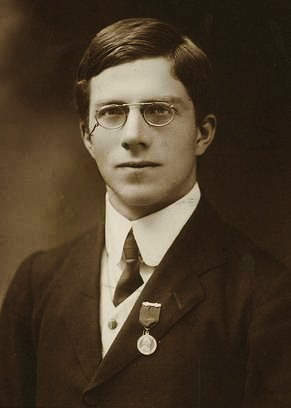
\includegraphics[width=0.9\columnwidth]{fisher.jpg}
		\end{column}
	\end{columns}
\end{frame}

\begin{frame}{$p = 0.06$}
	\begin{vfilleditems}
		\item Since $p$-value is a probability, it is also a continuous measure.
		\item There is no reason for us to differentiate $p = 0.049$ against $p = 0.051$.
		\item Robert Rosenthal, a psychologist said ``surely, God loves the $.06$ nearly as much as the $.05$''~\parencite{rosnow1989statistical}.
	\end{vfilleditems}
\end{frame}

\begin{frame}{But why I never heard about Bayesian statistics?\footnote{\textit{inverse probability}
			was how Bayes' theorem was called in the beginning of the 20th century}}
	\begin{columns}
		\begin{column}{0.8\textwidth}
			\begin{quotation}
				… it will be sufficient … to reaffirm my personal conviction …
				that the theory of inverse probability is founded upon an error,
				and must be wholly rejected.
			\end{quotation}
			\vfill \vfill
			\textcite{fisher1925statistical}
		\end{column}
		\begin{column}{0.2\textwidth}
			\centering
			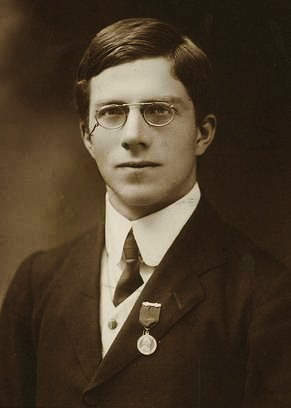
\includegraphics[width=0.9\columnwidth]{fisher.jpg}
		\end{column}
	\end{columns}
\end{frame}

\begin{frame}{Inside every nonBayesian, there is a Bayesian struggling to get out\footnote{
			quote from Dennis Lindley}}
	\begin{columns}
		\begin{column}{0.8\textwidth}
			\begin{vfilleditems}
				\item In his final year of life,
				Fisher published a paper \parencite{fisherExamplesBayesMethod1962}
				examining the possibilities of Bayesian methods,
				but with the prior probabilities being determined experimentally.
				\item Some authors speculate \parencite{jaynesProbabilityTheoryLogic2003}
				that if Fisher were alive today, he would probably be a Bayesian.
			\end{vfilleditems}
		\end{column}
		\begin{column}{0.2\textwidth}
			\centering
			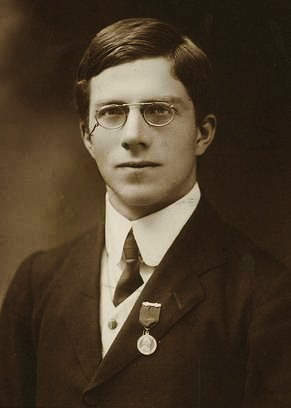
\includegraphics[width=0.9\columnwidth]{fisher.jpg}
		\end{column}
	\end{columns}
\end{frame}

\subsection{Bayesian Statistics}
\begin{frame}{Bayes' Theorem as an Inference Engine}
	\footnotesize Now that you know what is probability and Bayes' theorem,
	I will propose the following:
	$$
		\underbrace{P(\theta \mid y)}_{\text{Posterior}} = \frac{\overbrace{P(y \mid  \theta)}^{\text{Likelihood}} \cdot \overbrace{P(\theta)}^{\text{Prior}}}{\underbrace{P(y)}_{\text{Normalizing Constant}}}
	$$
	\begin{vfilleditems}
		\item \footnotesize $\theta$ -- parameter(s) of interest
		\item \footnotesize $y$ -- observed data
		\item \footnotesize \textbf{Priori}: prior probability of the parameter(s) value(s)
		\item \footnotesize \textbf{Likelihood}: probability of the observed data given the parameter(s) value(s)
		\item \footnotesize \textbf{Posterior}: posterior probability of the parameter(s) value(s) after we observed data $y$
		\item \footnotesize \textbf{Normalizing Constant}\footnote{sometimes also called \textit{evidence}.}: $P(y)$ does not make any intuitive sense.
		This probability is transformed and can be interpreted as something that only exists so that the result $P(y \mid \theta) P(\theta)$ be constrained between $0$ e $1$
		-- a valid probability.
	\end{vfilleditems}
\end{frame}

\begin{frame}{Bayes' Theorem as an Inference Engine}
	Bayesian statistics allows us to \textbf{quantify directly the uncertainty}
	related to the value of one or more parameters of our modelo given the
	observed data.
	This is the \textbf{main feature} of Bayesian statistics,
	since we are estimating directly $P(\theta \mid y)$ using Bayes' theorem.
	The resulting estimate is totally intuitive:
	simply quantifies the uncertainty that we have about the value of one or more
	parameters given the data, model assumptions (likelihood) and the prior
	probability of these parameter's values.
\end{frame}

\subsubsection{Advantages of Bayesian Statistics}
\begin{frame}{Bayesian vs Frequentist Stats}
	%\begin{table}[h!]
	\small
	\begin{tabular}{|l|p{.3\textwidth}|p{.3\textwidth}|}
		\toprule
		                     & \textcolor{blue}{\textbf{Bayesian Statistics}} & \textcolor{red}{\textbf{Frequentist Statistics}}                   \\ \midrule
		\textbf{Data}        & Fixed –- Non-random                            & Uncertain –- Random                                                \\ \midrule
		\textbf{Parameters}  & Uncertain –- Random                            & Fixed –- Non-random                                                \\ \midrule
		\textbf{Inference}   & Uncertainty regarding the parameter value      & Uncertainty regarding the sampling process from an infinite sample \\ \midrule
		\textbf{Probability} & Subjective                                     & Objective (but with several model assumptions)                     \\ \midrule
		\textbf{Uncertainty} & Posterior Interval –- $P(\theta \mid y)$       & Confidence Interval –- $P(y \mid \theta)$                          \\
		\bottomrule
	\end{tabular}
	%\end{table}
\end{frame}

\begin{frame}{Advantages of Bayesian Statistics}
	\begin{vfilleditems}
		\item Natural approach to express uncertainty
		\item Ability to incorporate previous information
		\item Higher model flexibility
		\item Full posterior distribution of the parameters
		\item Natural propagation of uncertainty
	\end{vfilleditems}
	\small \textbf{Main disadvantage}: Slow model fitting procedure
\end{frame}

\begin{frame}{The beginning of the end of Frequentist Statistics}
	\begin{vfilleditems}
		\small
		\item Know that you are in a very special moment in history of great changes in statistics
		\item I believe that frequentist statistics, specially the way we qualify evidence and hypotheses with
		$p$-values will transform in a ``significant''\footnote{pun intended ...} way.
		\item 6 years ago, the \textit{American Statistical Association} (ASA) published a declaration about
		$p$-values \parencite{Wasserstein2016}.
		It states exactly what we exposed here:
		The main concepts of the null hypothesis significant testing and,
		in particular $p$-values, cannot provide what researchers demand of them.
		Despite what says several textbooks, learning materials and published content,
		$p$-values below $0.05$ doesn't ``prove'' anything.
		Not, on the other way around, $p$-values higher than acima $0.05$ refute anything.
		\item ASA statement has more than 4.700 citations with relevant impact.
	\end{vfilleditems}
\end{frame}

\begin{frame}{The beginning of the end of Frequentist Statistics}
	\begin{vfilleditems}
		\small
		\item An international symposium was promoted in 2017 which originated an open-access special edition of
		\textit{The American Statistician} dedicated to practical ways to abandon $p < 0.05$
		\parencite{wassersteinMovingWorld052019}.
		\item Soon there were more attempts and claims.
		In September 2017, \textit{Nature Human Behaviour} published an editorial proposing that the $p$-value's
		significance level be decreased from $0.05$ to $0.005$ \parencite{benjaminRedefineStatisticalSignificance2018}.
		Several authors, including highly important and influential statisticians argued that this simple step would
		help to tackle the replication crisis problem in science, that many believe be the main consequence
		of the abusive use of $p$-values \parencite{Ioannidis2019}.
		\item Furthermore, many went a step ahead and suggested that science banish once for all $p$-values
		\parencite{ItTimeTalk2019,lakensJustifyYourAlpha2018}.
		Many suggest (including myself) that the main tool of statistical inference
		be Bayesian statistics \parencite{amrheinScientistsRiseStatistical2019, Goodman1180, vandeschootBayesianStatisticsModelling2021}.
	\end{vfilleditems}
\end{frame}

\section{Probability Distributions}

\subsection{Recommended References}
\begin{frame}{Probability Distributions - Recommended References}
	\begin{vfilleditems}
		\item \textcite{grimmettProbabilityRandomProcesses2020}
		\begin{vfilleditems}
			\item Chapter 3: Discrete random variables
			\item Chapter 4: Continuous random variables
		\end{vfilleditems}
		\item \textcite{dekkingModernIntroductionProbability2010}
		\begin{vfilleditems}
			\item Chapter 4: Discrete random variables
			\item Chapter 5: Continuous random variables
		\end{vfilleditems}
		\item \textcite{betancourtProbabilisticBuildingBlocks2019}
	\end{vfilleditems}
\end{frame}

%--- Intro -----------------------------------------------------------%
\begin{frame}{Probability Distributions}
	Bayesian statistics uses probability distributions as the inference
	engine of the parameter and uncertainty estimates.
	\vfill
	Imagine that probability distributions are small ``Lego'' pieces.
	We can construct anything we want with these little pieces.
	We can make a castle, a house, a city; literally anything.
	The same is valid for Bayesian statistical models.
	We can construct models from the simplest ones to the most complex
	using probability distributions and their relationships.
\end{frame}

\begin{frame}
	\begin{defn}[Probability Distribution Function]
		A probability distribution function is a mathematical function
		that outputs the probabilities for different results of an
		experiment.
		It is a mathematical description of a random phenomena in terms
		of its sample space and the event probabilities (subsets
		of the sample space).
		$$P(X): X \to \mathbb{R} \in [0, 1]$$
		For discrete random variables, we define as ``mass'',
		and for continuous random variables, we define as ``density''.
	\end{defn}
\end{frame}

\begin{frame}{Mathematical Notation}
	We use the notation
	$$X \sim \text{Dist}(\theta_1, \theta_2, \dots)$$
	where:
	\begin{vfilleditems}
		\item $X$: random variable
		\item Dist: distribution name
		\item $\theta_1, \theta_2, \dots$: parameters that define how the
		distribution behaves
	\end{vfilleditems}
	Every probability distribution can be ``parameterized'' by specifying
	parameters that allow to control certain distribution aspects for
	a specific goal.
\end{frame}

\begin{frame}{Probability Distribution Function}
	\centering
	\begin{tikzpicture}
		\begin{axis}[every axis plot, line width=2pt,
				ylabel=FDP,
				xlabel={$X$},
				domain=-4:4,samples=200,
				axis x line*=bottom, % no box around the plot, only x and y axis
				axis y line*=left, % the * suppresses the arrow tips
				enlarge x limits=true, % extend the axes a bit
			]

			\addplot [blue] {gaussian(0, 1)};
		\end{axis}
	\end{tikzpicture}
\end{frame}

\begin{frame}
	\begin{defn}[Cumulative Distribution Function]
		The cumulative distribution function (CDF) of a random variable
		$X$ evaluated at $x$ is the probability that $X$ will take
		values less or qual than $x$:
		$$\text{CDF} = P(X \leq x)$$
	\end{defn}
\end{frame}

\begin{frame}{Cumulative Distribution Function}
	\centering
	\begin{tikzpicture}
		\begin{axis}[every axis plot, line width=2pt,
				ylabel=CDF,
				xlabel={$X$},
				domain=-4:4,samples=200,
				axis x line*=bottom, % no box around the plot, only x and y axis
				axis y line*=left, % the * suppresses the arrow tips
				enlarge x limits=true, % extend the axes a bit
			]

			\addplot [blue] {normcdf(0, 1)};
		\end{axis}
	\end{tikzpicture}
\end{frame}

%--- Discrete --------------------------------------------------------%
\subsection{Discrete Distributions}
\begin{frame}
	\begin{defn}[Discrete Distributions]
		Discrete probability distributions are distributions which the
		results are a discrete number:
		$-N, \dots, -2, 1, 0,1,2,\dots, N$ e $N \in \mathbb{Z}$.
		In discrete probability distributions we call the probability
		of a distribution taking certain values as ``mass''.
		The probability mass function (PMF) is the function that
		specifies the probability of a random variable $X$ taking value $x$:
		$$\text{PMF}(x) = P(X = x)$$
	\end{defn}
\end{frame}

\subsubsection{Discrete Uniform}
\begin{frame}{Discrete Uniform}
	The discrete uniform is a symmetric probability distribution in which
	a finite number of values are equally likely of being observable.
	Each one of the $n$ values have probability $\frac{1}{n}$.
	\vfill
	The uniform discrete distribution has two parameters and its notation is
	$\text{Uniform}(a, b)$:
	\begin{vfilleditems}
		\item $a$ -- lower bound
		\item $b$ -- upper bound
	\end{vfilleditems}
	\vfill
	Example: dice.
\end{frame}

\begin{frame}{Discrete Uniform}
	$$\text{Uniform}(a,b) = f(x, a, b) = \frac{1}{b-a+1} \text{ for $a \leq x \leq b$ and $x\in \{a,a+1,\dots ,b-1,b\}$}$$
\end{frame}

\begin{frame}{Discrete Uniform}
	\centering
	\begin{tikzpicture}
		\begin{axis}[every axis plot,
				ybar=0pt, bar width=0.3,
				ylabel=PMF,
				samples at={1,...,6}, % All plots: from 1:6, 6 samples only
				axis x line*=bottom, % no box around the plot, only x and y axis
				axis y line*=left, % the * suppresses the arrow tips
				enlarge x limits=true, % extend the axes a bit
			]

			\addplot [fill=blue] {discreteuniform(1, 6)};
			\addlegendentry{$a=1, b=6$}
		\end{axis}
	\end{tikzpicture}
\end{frame}

\subsubsection{Bernoulli}
\begin{frame}{Bernoulli}
	Bernoulli distribution describes a binary event of the success of an experiment.
	We represent $0$ as failure and $1$ as success, hence the result of a
	Bernoulli distribution is a binary variable $Y \in \{0, 1\}$.
	\vfill
	Bernoulli distribution is often used to model binary discrete results
	where there is only two possible results.
	\vfill
	Bernoulli distribution has only a single parameter and its notation is
	$\text{Bernoulli} (p)$:
	\begin{vfilleditems}
		\item $p$ -- probability of success
	\end{vfilleditems}
	\vfill
	Example: If the patient survived or died or if the client purchased or not.
\end{frame}

\begin{frame}{Bernoulli}
	$$\text{Bernoulli}(p) = f(x, p)=p^{x}(1-p)^{1-x} \text{ for $x \in \{0,1\}$}$$ %
\end{frame}

\begin{frame}{Bernoulli}
	\centering
	\begin{tikzpicture}
		\begin{axis}[every axis plot,
				ybar=0pt, bar width=0.5,
				ymin=0,
				xmin=-0.25, xmax=1.25,
				ylabel=PMF,
				axis x line*=bottom, % no box around the plot, only x and y axis
				axis y line*=left, % the * suppresses the arrow tips
				enlarge x limits=true, % extend the axes a bit
				xtick={0, 1}
			]

			\addplot [fill=blue] coordinates {
					(0, 0.6)
					(1, 0.4)};
			\addlegendentry{$p=\frac{1}{3}$}
		\end{axis}
	\end{tikzpicture}
\end{frame}

\subsubsection{Binomial}
\begin{frame}{Binomial}
	The binomial distribution describes an event in which the number of
	successes in a sequence $n$ independent experiments,
	each one making a yes--no question with probability of success $p$.
	Notice that Bernoulli distribution is a special case of the binomial
	distribution where $n=1$.
	\vfill
	The binomial distribution has two parameters and its notation is
	$\text{Binomial}(n, p)$ :
	\begin{vfilleditems}
		\item $n$ -- number of experiments
		\item $p$ -- probability of success
	\end{vfilleditems}
	\vfill
	Example: number of heads in five coin throws.
\end{frame}

\begin{frame}{Binomial}
	$$\text{Binomial}(n,p) = f(x, n, p) = \binom{n}{x}p^{x}(1-p)^{n-x} \text{ for $x \in \{0, 1, \dots, n\}$}$$
\end{frame}

\begin{frame}{Binomial}
	\centering
	\begin{tikzpicture}
		\begin{axis}[every axis plot,
				ybar=0pt, bar width=1,
				ylabel=PMF,
				ytick={0,0.05,...,0.15},
				samples at={0,...,40},
				axis x line*=bottom, % no box around the plot, only x and y axis
				axis y line*=left, % the * suppresses the arrow tips
				enlarge x limits=true, % extend the axes a bit
				y tick label style={/pgf/number format/.cd, fixed, fixed zerofill, precision=2}
			]

			\addplot [fill=blue, fill opacity=0.5] {binomial(40, 0.2)};
			\addlegendentry{$n=40, p=\frac{1}{5}$}
			\addplot [fill=red, fill opacity=0.5] {binomial(40, 0.5)};
			\addlegendentry{$n=40, p=\frac{1}{2}$}
		\end{axis}
	\end{tikzpicture}
\end{frame}

\subsubsection{Poisson}
\begin{frame}{Poisson}
	Poisson distribution describes the probability of a certain number of
	events occurring in a fixed time interval if these events
	occur with a constant mean rate which is known and independent since
	the time of last occurrence.
	Poisson distribution can also be used for number of events in other
	type of intervals, such as distance, area or volume.
	\vfill
	Poisson distribution has one parameter and its notation is $\text{Poisson}(\lambda)$:
	\begin{vfilleditems}
		\item $\lambda$ -- rate
	\end{vfilleditems}
	\vfill
	Example: number of e-mails that you receive daily or the number of the potholes you'll find in your commute.
\end{frame}

\begin{frame}{Poisson}
	$$\text{Poisson}(\lambda) = f(x, \lambda) = \frac{\lambda^x e^{-\lambda}}{x!} \text{ for $\lambda > 0$}$$
\end{frame}

\begin{frame}{Poisson}
	\centering
	\begin{tikzpicture}
		\begin{axis}[every axis plot,
				ybar=0pt, bar width=1,
				ylabel=PMF,
				samples at={0,...,8},
				axis x line*=bottom, % no box around the plot, only x and y axis
				axis y line*=left, % the * suppresses the arrow tips
				enlarge x limits=true, % extend the axes a bit
			]

			\addplot [fill=blue, fill opacity=0.5] {poisson(1)};
			\addlegendentry{$\lambda=2$}
			\addplot [fill=red, fill opacity=0.5] {poisson(4)};
			\addlegendentry{$\lambda=4$}
		\end{axis}
	\end{tikzpicture}
\end{frame}

\subsubsection{Negative Binomial}
\begin{frame}{Negative Binomial\footnote{
			any phenomena that can be modeles as a Poisson distribution can be
			modeled also as negative binomial distribution
			\parencite{gelman2013bayesian, gelman2020regression}.}}
	\small
	The binomial distribution describes an event in which the number of
	successes in a sequence $n$ independent experiments,
	each one making a yes--no question with probability of success $p$
	until $k$ successes.
	Notice that it becomes the Poisson distribution in the limit as $k \to \infty$.
	This makes it a robust option to replace a Poisson distribution to model
	phenomena with overdispersion
	(presence of greater variability in data than would be expected).
	\vfill \small
	The negative binomial has two parameters and its notation is
	$\text{Negative Binomial}(k, p)$:
	\begin{vfilleditems}
		\small
		\item $k$ -- number of successes
		\item $p$ -- probability of success
	\end{vfilleditems}
	\vfil \small
	Example: annual occurrence of tropical cyclones.
\end{frame}

\begin{frame}{Negative Binomial}
	$$
		\begin{aligned}
			\text{Negative Binomial}(k, p) & = f(x, k, p) & = \binom{x + k - 1}{k - 1}p^{x}(1-p)^{k} \\
			\\
			                               & ~            & \text{for $x \in \{0, 1, \dots, n\}$}
		\end{aligned}
	$$
\end{frame}

\begin{frame}{Negative Binomial}
	\centering
	\begin{tikzpicture}
		\begin{axis}[every axis plot,
				ybar=0pt, bar width=1,
				ylabel=PMF,
				samples at={0,...,8},
				axis x line*=bottom, % no box around the plot, only x and y axis
				axis y line*=left, % the * suppresses the arrow tips
				enlarge x limits=true, % extend the axes a bit
			]

			\addplot [fill=blue, fill opacity=0.5] {negativebinomial(1, 0.5)};
			\addlegendentry{$k=1, p=\frac{1}{2}$}
			\addplot [fill=red, fill opacity=0.5] {negativebinomial(5,0.5)};
			\addlegendentry{$k=5, p=\frac{1}{2}$}
		\end{axis}
	\end{tikzpicture}
\end{frame}

%--- Continuous ------------------------------------------------------%

\subsection{Continuous Distributions}
\begin{frame}
	\begin{defn}[Continuous Distributions]
		\small
		Continuous probability distributions are distributions which
		the results are values in a continuous real number line:
		$(-\infty, +\infty) \in \mathbb{R}$.
		In continuous probability distributions we call the probability
		of a distribution taking values as ``density''.
		Since we are referring to real numbers we cannot obtain the
		probability of a random variable $X$ taking exactly the value $x$.
		This will always be $0$, since we cannot specify the exact
		value of $x$. $x$ lies in the real number line, hence,
		we need to specify the probability of $X$ taking values in an
		interval $[a,b]$.
		The probability density function (PDF) is defined as:
		$$\text{FDP}(x) = P(a \leq X \leq b) = \int_a^b f(x) dx$$
	\end{defn}
\end{frame}

\subsubsection{Continuous Uniform}
\begin{frame}{Continuous Uniform}
	The continuous uniform distribution is a symmetric probability distribution
	in which an infinite number of value intervals are equally likely of being observable.
	Each one of the infinite $n$ intervals have probability $\frac{1}{n}$.
	\vfill
	The continuous uniform distribution has two parameters and its notation is $\text{Uniform}(a, b)$:
	\begin{vfilleditems}
		\item $a$ -- lower bound
		\item $b$ -- upper bound
	\end{vfilleditems}
\end{frame}

\begin{frame}{Continuous Uniform}
	$$\text{Uniform}(a,b) = f(x, a, b) = \frac{1}{b-a} \text{ for $a \leq x \leq b$ e $x \in [a, b]$}$$
\end{frame}

\begin{frame}{Continuous Uniform}
	\centering
	\begin{tikzpicture}
		\begin{axis}[every axis plot, line width=2pt,
				ylabel=PDF,
				domain=0:6,samples=200,
				axis x line*=bottom, % no box around the plot, only x and y axis
				axis y line*=left, % the * suppresses the arrow tips
				enlarge x limits=true, % extend the axes a bit
			]

			\addplot [blue] {continuousuniform(0, 6)};
			\addlegendentry{$a=0, b=6$}
		\end{axis}
	\end{tikzpicture}
\end{frame}

\subsubsection{Normal}
\begin{frame}{Normal}
	This distribution is generally used in social and natural sciences to
	represent continuous variables in which its underlying distribution are unknown.
	This assumption is due to the central limit theorem (CLT) that,
	under precise conditions, the mean of many samples (observations) of a
	random variable with finite mean and variance is itself a random variable
	which the underlying distribution converges to a normal distribution
	as the number of samples increases (as $n \to \infty$).
	\vfill
	Hence, physical quantities that we assume that are the sum of many
	independent processes (with measurement error) often have underlying
	distributions that are similar to normal distributions.
\end{frame}

\begin{frame}{Normal}
	The normal distribution has two parameters and its notation is
	$\text{Normal}(\mu, \sigma^2)$ or $\text{N}(\mu, \sigma^2)$:
	\begin{vfilleditems}
		\item $\mu$ -- mean of the distribution, and also median and mode
		\item $\sigma$ -- standard deviation\footnote{sometimes is also parametrized as variance $\sigma^2$.},
		a dispersion measure of how observations occur in relation from the mean
	\end{vfilleditems}
	\vfill
	Example: height, weight etc.
\end{frame}

\begin{frame}{Normal\footnote{
	see how the normal distribution was derived from the binomial
	distribution in the \hyperlink{appendixnormal}{backup slides}.}}
	$$\text{Normal}(\mu,\sigma) = f(x, \mu, \sigma) = \frac{1}{\sigma{\sqrt{2\pi }}}e^{-{\frac{1}{2}}\left({\frac {x-\mu }{\sigma }}\right)^{2}} \text{ for $\sigma > 0$}$$
\end{frame}

\begin{frame}{Normal}
	\centering
	\begin{tikzpicture}
		\begin{axis}[every axis plot, line width=2pt,
				ylabel=PDF,
				domain=-4:6,samples=200,
				axis x line*=bottom, % no box around the plot, only x and y axis
				axis y line*=left, % the * suppresses the arrow tips
				enlarge x limits=true, % extend the axes a bit
			]

			\addplot [blue] {gaussian(0, 1)};
			\addlegendentry{$\mu=0, \sigma=1$}
			\addplot [red] {gaussian(0, 2)};
			\addlegendentry{$\mu=0, \sigma=2$}
			\addplot [yellow] {gaussian(2, 1)};
			\addlegendentry{$\mu=2, \sigma=1$}
		\end{axis}
	\end{tikzpicture}
\end{frame}

\subsubsection{Log-Normal}
\begin{frame}{Log-Normal}
	The log-normal distribution is a continuous probabiity distribution of a
	random variable which its natural logarithm is distributed as a normal distribution.
	Thus, if the natural logarithm a random variable $X$, $\ln(X)$, is distributed
	as a normal distribution, then $Y = \ln(X)$ is normally distributed and
	$X$ is log-normally distributed.
	\vfill
	A a log-normal random variable only takes positive real values.
	It is a convenient and useful model for measurements in exact and engineering
	sciences, as well as in biomedical, economical and other sciences.
	For example, energy, concentrations, length, finantial returns and other measurements.
	\vfill
	A log-normal process is the statistical realization of a multiplicative
	product of many indepedent positive random variables.
\end{frame}

\begin{frame}{Log-Normal}
	The log-normal distribution has two parameters and its notation is
	$\text{Log-Normal}(\mu, \sigma^2)$:
	\begin{vfilleditems}
		\item $\mu$ -- mean of the distribution's natural logarithm
		\item $\sigma$ -- square root of the variance of the distribution's natural logarithm
	\end{vfilleditems}
\end{frame}

\begin{frame}{Log-Normal}
	$$\text{Log-Normal}(\mu,\sigma) = f(x, \mu, \sigma) = \frac{1}{x \sigma{\sqrt{2\pi}}}e^{-\left({\frac {(\ln(x)-\mu)^2}{2 \sigma^2 }}\right)} \text{ for $\sigma > 0$}$$
\end{frame}

\begin{frame}{Log-Normal}
	\centering
	\begin{tikzpicture}
		\begin{axis}[every axis plot, line width=2pt,
				ylabel=PDF,
				domain=0:5,samples=200,
				axis x line*=bottom, % no box around the plot, only x and y axis
				axis y line*=left, % the * suppresses the arrow tips
				enlarge x limits=true, % extend the axes a bit
			]

			\addplot [blue] {lognormal(0, 0.25)};
			\addlegendentry{$\mu=0, \sigma=\frac{1}{4}$}
			\addplot [red] {lognormal(0, 1)};
			\addlegendentry{$\mu=0, \sigma=1$}
			\addplot [yellow] {lognormal(1, 1)};
			\addlegendentry{$\mu=1, \sigma=1$}
		\end{axis}
	\end{tikzpicture}
\end{frame}

\subsubsection{Exponential}
\begin{frame}{Exponential}
	The exponential distribution is the probability distribution of the time
	between events that occurs in a continous manner, are indepedent,
	and have constant mean rate of occurrence.
	\vfill
	The exponential distribution has one parameter and its notation is
	$\text{Exponential}(\lambda)$:
	\begin{vfilleditems}
		\item $\lambda$ -- rate
	\end{vfilleditems}
	\vfill
	Example: How long until the next earthquake or how long until the next bus arrives.
\end{frame}

\begin{frame}{Exponential}
	$$\text{Exp}(\lambda) = f(x, \lambda) = \lambda e^{-\lambda x} \text{ for $\lambda > 0$}$$
\end{frame}

\begin{frame}{Exponential}
	\centering
	\begin{tikzpicture}
		\begin{axis}[every axis plot, line width=2pt,
				ylabel=PDF,
				domain=0:5,samples=200,
				axis x line*=bottom, % no box around the plot, only x and y axis
				axis y line*=left, % the * suppresses the arrow tips
				enlarge x limits=true, % extend the axes a bit
			]

			\addplot [blue] {exponential(0.5)};
			\addlegendentry{$\lambda=\frac{1}{2}$}
			\addplot [red] {exponential(1)};
			\addlegendentry{$\lambda=1$}
			\addplot [yellow] {exponential(2)};
			\addlegendentry{$\lambda=2$}
		\end{axis}
	\end{tikzpicture}
\end{frame}

\subsubsection{Student's $t$}
\begin{frame}{Student's $t$}
	Student's $t$ distribution arises by estimating the mean of a normally-distributed
	population in situations where the sample size is small and the standard
	devation is known\footnote{this is where the ubiquous Student's $t$ test.}.
	\vfill
	If we take a sample of $n$ observations from a normal distribution,
	then Student's $t$ distribution with $\nu = n-1$ degrees of freedom can
	be defined as the distribution of the location of the sample mean
	in relation to the true mean, divided by the sample's standard deviation,
	after multiplying by the scaling term $\sqrt{n}$.
	\vfill
	Student's $t$ distribution is symmetric and in a bell-shape,
	like the normal distribution, but with long tails,
	which means that has more chance to produce values far away from its mean.
\end{frame}

\begin{frame}{Student's $t$}
	Student's $t$ distribution has one parameter and its notation is
	$\text{Student}(\nu)$:
	\begin{vfilleditems}
		\item $\nu$ -- degrees of freedom, controls how much it resembles a normal distribution
	\end{vfilleditems}
	\vfill
	Example: a dataset full of outliers.
\end{frame}

\begin{frame}{Student's $t$}
	$$\text{Student}(\nu) = f(x, \nu) = \frac{\Gamma \left(\frac{\nu+1}{2} \right)} {\sqrt{\nu\pi}\,\Gamma \left(\frac{\nu}{2} \right)} \left(1+\frac{x^2}{\nu} \right)^{-\frac{\nu+1}{2}} \text{ for $\nu \geq 1$}$$
\end{frame}

\begin{frame}{Student's $t$}
	\centering
	\begin{tikzpicture}
		\begin{axis}[every axis plot, line width=2pt,
				ylabel=PDF,
				domain=-4:4,samples=200,
				axis x line*=bottom, % no box around the plot, only x and y axis
				axis y line*=left, % the * suppresses the arrow tips
				enlarge x limits=true, % extend the axes a bit
			]

			\addplot [blue] {student(1)};
			\addlegendentry{$\nu=1$}
			\addplot [red] {student(3)};
			\addlegendentry{$\nu=3$}
			\addplot [yellow] {student(30)};
			\addlegendentry{$\nu=30$}
		\end{axis}
	\end{tikzpicture}
\end{frame}

\subsubsection{Beta}
\begin{frame}{Beta}
	The beta distribution is a natural choice to model anything that is
	restricted to values between $0$ e $1$.
	Hence, it is a good candidate to model probabilities and proportions.
	\vfill
	The beta distribution has two parameters and its notations is
	$\text{Beta} (\alpha, \beta)$:
	\begin{vfilleditems}
		\item $\alpha$ or sometimes $a$ -- shape parameter,
		controls how much the shape is shifted towards $1$
		\item $\beta$ or sometimes $b$ -- shape parameter,
		controls how much the shape is shifted towards $0$
	\end{vfilleditems}
	\vfill
	Example: A basketball player that has already scored 5 free throws and
	missed 3 in a total of 8 attempts -- $\text{Beta}(3, 5)$
\end{frame}

\begin{frame}{Beta}
	$$\text{Beta} (\alpha, \beta) = f(x, \alpha, \beta) \frac{x^{\alpha-1}(1-x)^{\beta-1}} {\frac{\Gamma (\alpha )\Gamma (\beta )}{\Gamma (\alpha +\beta )}} \text{ for $\alpha,\beta > 0$ and $x \in [0, 1]$}$$
\end{frame}

\begin{frame}{Beta}
	\centering
	\begin{tikzpicture}
		\begin{axis}[every axis plot, line width=2pt,
				ylabel=PDF,
				domain=0:1,samples=200,
				axis x line*=bottom, % no box around the plot, only x and y axis
				axis y line*=left, % the * suppresses the arrow tips
				enlarge x limits=true, % extend the axes a bit
			]

			\addplot [blue] {beta(1,1)};
			\addlegendentry{$\alpha=\beta=1$}
			\addplot [red] {beta(3,2)};
			\addlegendentry{$\alpha=3,\beta=2$}
			\addplot [yellow] {beta(2,3)};
			\addlegendentry{$\alpha=2,\beta=3$}
		\end{axis}
	\end{tikzpicture}
\end{frame}

\section{Priors}

\subsection{Recommended References}
\begin{frame}{Priors and Posteriors - Recommended References}
	\begin{vfilleditems}
		\item \textcite{gelman2013bayesian}:
		\begin{vfilleditems}
			\item Chapter 2: Single-parameter models
			\item Chapter 3: Introduction to multiparameter models
		\end{vfilleditems}
		\item \textcite{mcelreath2020statistical} - Chapter 4: Geocentric Models
		\item \textcite{gelman2020regression}:
		\begin{vfilleditems}
			\item Chapter 9, Section 9.3: Prior information and Bayesian synthesis
			\item Chapter 9, Section 9.5: Uniform, weakly informative, and informative priors in regression
		\end{vfilleditems}
		\item \textcite{vandeschootBayesianStatisticsModelling2021}
	\end{vfilleditems}
\end{frame}

\begin{frame}{Prior Probability }
	Bayesian statistics is characterized by the use of prior information
	as the prior probability $P(\theta)$, often just prior:
	$$
		\underbrace{P(\theta \mid y)}_{\text{Posterior}} = \frac{\overbrace{P(y \mid  \theta)}^{\text{Likelihood}} \cdot \overbrace{P(\theta)}^{\text{Prior}}}{\underbrace{P(y)}_{\text{Normalizing Constant}}}
	$$
\end{frame}

\subsection{The subjectivity of the Prior}
\begin{frame}{The subjectivity of the Prior}
	\begin{vfilleditems}
		\item Many critics to Bayesian statistics are due the subjectivity
		in eliciting priors probability on certain hypothesis or model parameter's
		values.
		\item Subjectivity is something unwanted in the ideal picture of the
		scientist and the scientific method.
		\item Anything that involves human action will never be free from
		subjectivity.
		We have subjectivity in everything and science is \textcolor{red}{no} exception.
		\item The creative and deductive process of theory and hypotheses formulations
		is \textbf{not} objective.
		\item Frequentist statistics, which bans the use of prior probabilities
		is also subjective, since there is \textbf{A LOT} of subjectivity in
		choosing which model and likelihood function \parencite{jaynesProbabilityTheoryLogic2003, vandeschootBayesianStatisticsModelling2021}
	\end{vfilleditems}
\end{frame}

\begin{frame}{How to Incorporate Subjectivity}
	\begin{vfilleditems}
		\item Bayesian statistics \textbf{embraces} subjectivity while
		frequentist statistics \textbf{bans} it.
		\item For Bayesian statistics, \textbf{subjectivity guides our inferences}
		and leads to more robust and reliable models that can assist in
		decision making.
		\item Whereas, for frequentist statistics, \textbf{subjectivity is a taboo}
		and all inferences should be objective,
		even if it resorts to \textbf{hiding and omitting model assumptions}.
		\item Bayesian statistics also has assumptions and subjectivity,
		but these are \textbf{declared and formalized}
	\end{vfilleditems}
\end{frame}

\subsection{Types of Priors}

\begin{frame}{Types of Priors}
	In general, we can have 3 types of priors in a Bayesian approach
	\parencite{gelman2013bayesian, mcelreath2020statistical, vandeschootBayesianStatisticsModelling2021}:
	\begin{vfilleditems}
		\item \textbf{uniform (flat)}: not recommended.
		\item \textbf{weakly informative}: small amounts of real-world information
		along with common sense and low specific domain knowledge added.
		\item \textbf{informative}: introduction of medium to high domain knowledge.
	\end{vfilleditems}
\end{frame}

\subsubsection{Uniform Prior (Flat)}
\begin{frame}{Uniform Prior (Flat)}
	Starts from the premise that ``everything is possible''.
	There is no limits in the degree of beliefs that the distribution of certain
	values must be or any sort of restrictions.
	\vfill
	Flat and super-vague priors are not usually recommended and some thought
	should included to have at least weakly informative priors.
	\vfill
	Formally, an uniform prior is an uniform distribution over all the
	possible support of the possible values:
	\begin{vfilleditems}
		\item \textbf{model parameters}: $\{\theta \in \mathbb{R} : -\infty < \theta < \infty\}$
		\item \textbf{model error or residuals}: $\{\sigma \in \mathbb{R}^+ : 0 \leq \theta < \infty\}$
	\end{vfilleditems}
\end{frame}

\subsubsection{Weekly Informative Prior}
\begin{frame}{Weekly Informative Prior}
	Here we start to have ``educated'' guess about our parameter values.
	Hence, we don't start from the premise that ``anything is possible''.
	\vfill
	I recommend always to transform the priors of the problem at hand into
	something centered in $0$ with standard deviation of $1$\footnote{
		this is called standardization,
		transforming all variables into $\mu=0$ and $\sigma=1$.}:
	\vfill
	\begin{vfilleditems}
		\item $\theta \sim \text{Normal}(0, 1)$ (Andrew Gelman's preferred choice\footnote{
			see more about prior choices in the
			\href{https://github.com/stan-dev/stan/wiki/Prior-Choice-Recommendations}{\texttt{Stan}'s GitHub wiki}.})
		\item $\theta \sim \text{Student}(\nu=3, 0, 1)$ (Aki Vehtari's preferred choice)
	\end{vfilleditems}
\end{frame}

\begin{frame}{An Example of a Robust Prior}
	\small
	A nice example comes from a Ben Goodrich's lecture\footnote{
		\url{https://youtu.be/p6cyRBWahRA},
		in case you want to see the full video,
		the section about priors related to the argument begins at minute 40}
	(Columbia professor and member of \texttt{Stan}'s research group.
	\vfill
	He discuss about one of the biggest effect sizes observed in social sciences.
	In the exit pools for the 2008 USA presidential election (Obama vs McCain),
	there was, in general, around 40\% of support for Obama.
	If you changed the respondent race from non-black to black,
	this was associated with an increase of 60\% in the probability of the respondent
	to vote on Obama
	\vfill
	In logodds scales, 2.5x increase (from 40\% to almost 100\%) would be equivalent,
	on a bernoulli/logistic/binomial model,
	to a coefficient value of $\approx 0.92$\footnote{
		$\log(\text{odds ratio}) = \log(2.5) = 0.9163$.}.
	This effect size would be easily derived from a $\text{Normal}(0, 1)$ prior.
\end{frame}

\subsubsection{Informative Prior}
\begin{frame}{Informative Prior}
	In some contexts, it is interesting to use an informative prior.
	Good candidates are when data is scarce or expensive and prior knowledge
	about the phenomena is available.
	\vfill
	Some examples:
	\begin{vfilleditems}
		\item $\text{Normal}(5, 20)$
		\item $\text{Log-Normal}(0, 5)$
		\item $\text{Beta}(100, 9803)$\footnote{
			this is used in COVID-19 models from the
			\href{https://codatmo.github.io}{CoDatMo} \texttt{Stan}
			research group.}
	\end{vfilleditems}
\end{frame}

\section{Predictive Checks}

\subsection{Recommended References}
\begin{frame}{Predictive Checks - Recommended References}
	\begin{vfilleditems}
		\item \textcite{gelman2013bayesian} - Chapter 6: Model checking
		\item \textcite{mcelreath2020statistical} - Chapter 5: Geocentric Models
		\item \textcite{gelman2020regression}:
		\begin{vfilleditems}
			\item Chapter 6: Background on regression modeling
			\item Chapter 11: Assumptions, diagnostics, and model evaluation
		\end{vfilleditems}
		\item \textcite{gelmanBayesianWorkflow2020}
	\end{vfilleditems}
\end{frame}

\subsection{All models are wrong}
\begin{frame}{All models are wrong}
	\begin{columns}
		\begin{column}{0.8\textwidth}
			\begin{quotation}
				All models are wrong but some are useful
			\end{quotation}
			\vfill
			\textcite{boxScienceStatistics1976}
		\end{column}
		\begin{column}{0.2\textwidth}
			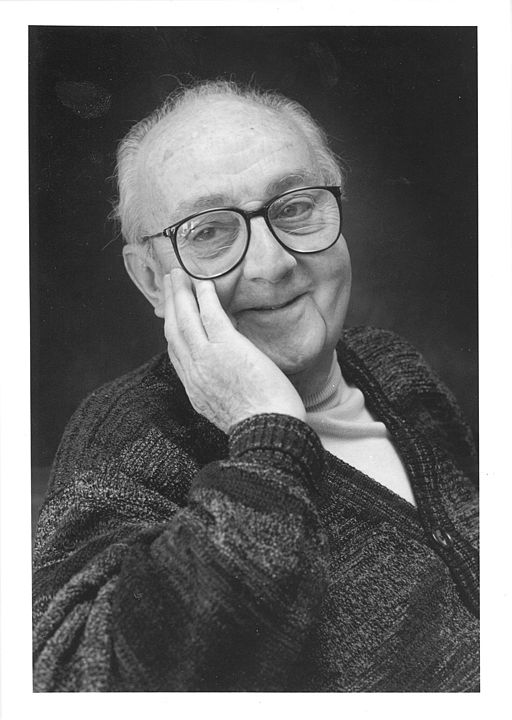
\includegraphics[width=0.9\columnwidth]{george_box.jpg}
		\end{column}
	\end{columns}
\end{frame}

\subsection{Bayesian Workflow}
\begin{frame}{Bayesian Workflow\footnote{based on \textcite{gelmanBayesianWorkflow2020}}}
	\centering
	\begin{tikzpicture}[
			scale=0.8,
			transform shape, thick,
			every node/.style={text width=3.5cm, align=center},
			constructs/.style = {draw,
					ellipse,
					minimum width=4cm,
					minimum height=2cm}
		]
		\node[constructs] (Model) {Model Specification};
		\node[constructs] [right = of Model] (Prior) {Prior Elicitation};
		\node[constructs] [right = of Prior] (Posterior) {Posterior Inference};
		\draw [<->, line width=1pt] (Model) to [out=45,in=135] node[above] {\textit{Prior Predictive Check}} (Prior);
		%\draw [->, line width=1pt] (Prior) to [out=225,in=315] {} (Model);
		\draw [<->, line width=1pt] (Prior) to [out=45,in=135] node[above] {\textit{Posterior Predictive Check}} (Posterior);
		%\draw [->, line width=1pt] (Posterior) to [out=225,in=315] {} (Prior);
	\end{tikzpicture}
\end{frame}

\begin{frame}{Bayesian Workflow\footnote{
			adapted from \href{https://github.com/elizavetasemenova}
			{Elizaveta Semenova}.}}
	\begin{vfilleditems}
		\item Understand the domain and problem.
		\item Formulate the model mathematically.
		\item Implement model, test, and debug.
		\item Perform prior predictive checks.
		\item Fit the model.
		\item Assess convergence diagnostics.
		\item Perform posterior predictive checks.
		\item Improve the model iteratively: from baseline to complex and computationally efficient models.
	\end{vfilleditems}

\end{frame}

\begin{frame}{Actual Bayesian Workflow}
	\centering
	\begin{figure}
		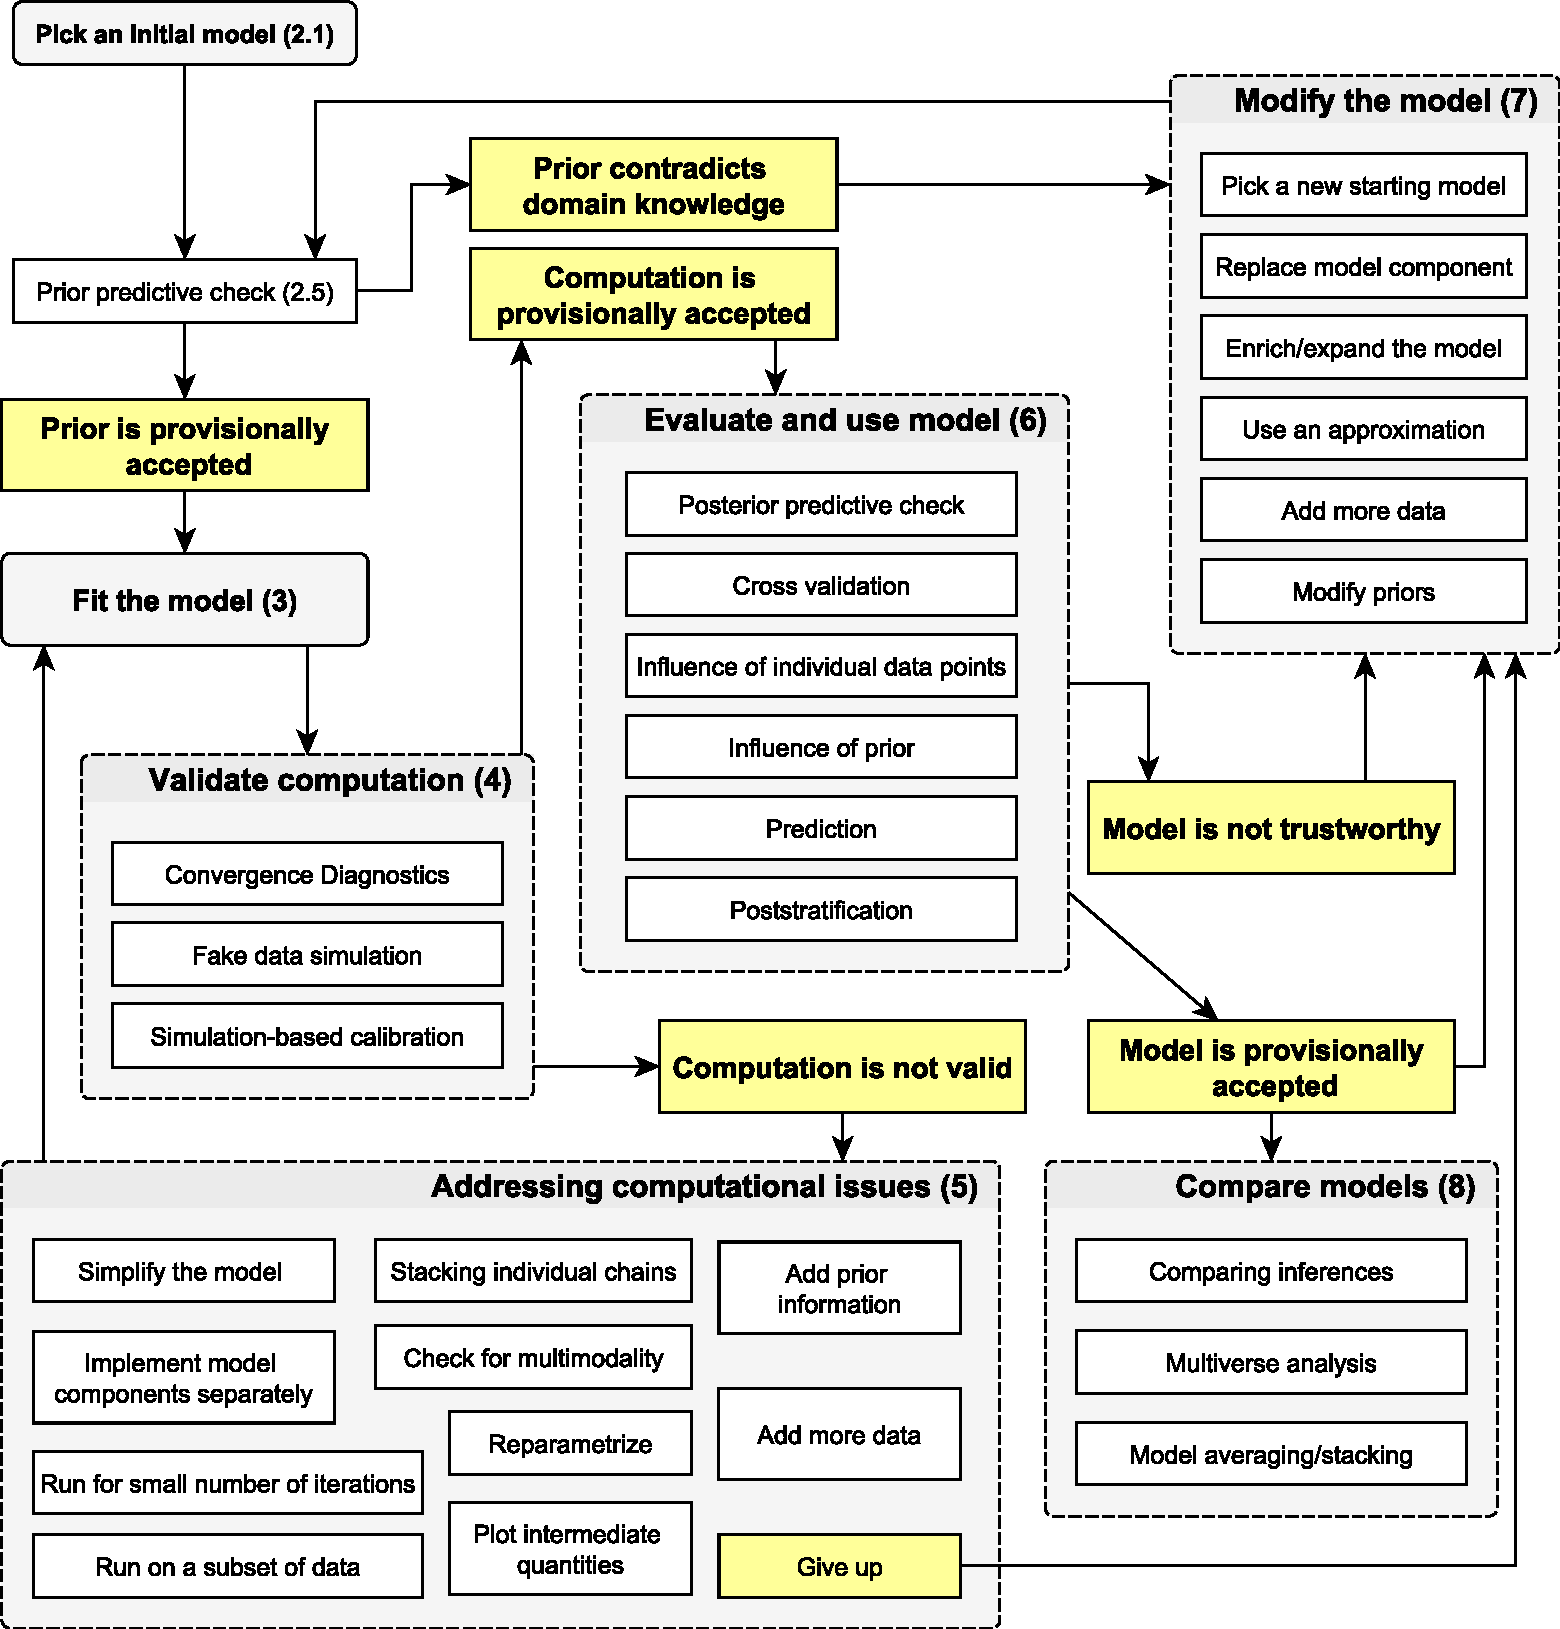
\includegraphics[height=0.75\textheight]{workflow_overview.pdf}
		\caption{Bayesian workflow by \textcite{gelmanBayesianWorkflow2020}}
	\end{figure}
\end{frame}

\begin{frame}{Not a ``new ideia''...}
	\centering
	\begin{figure}
		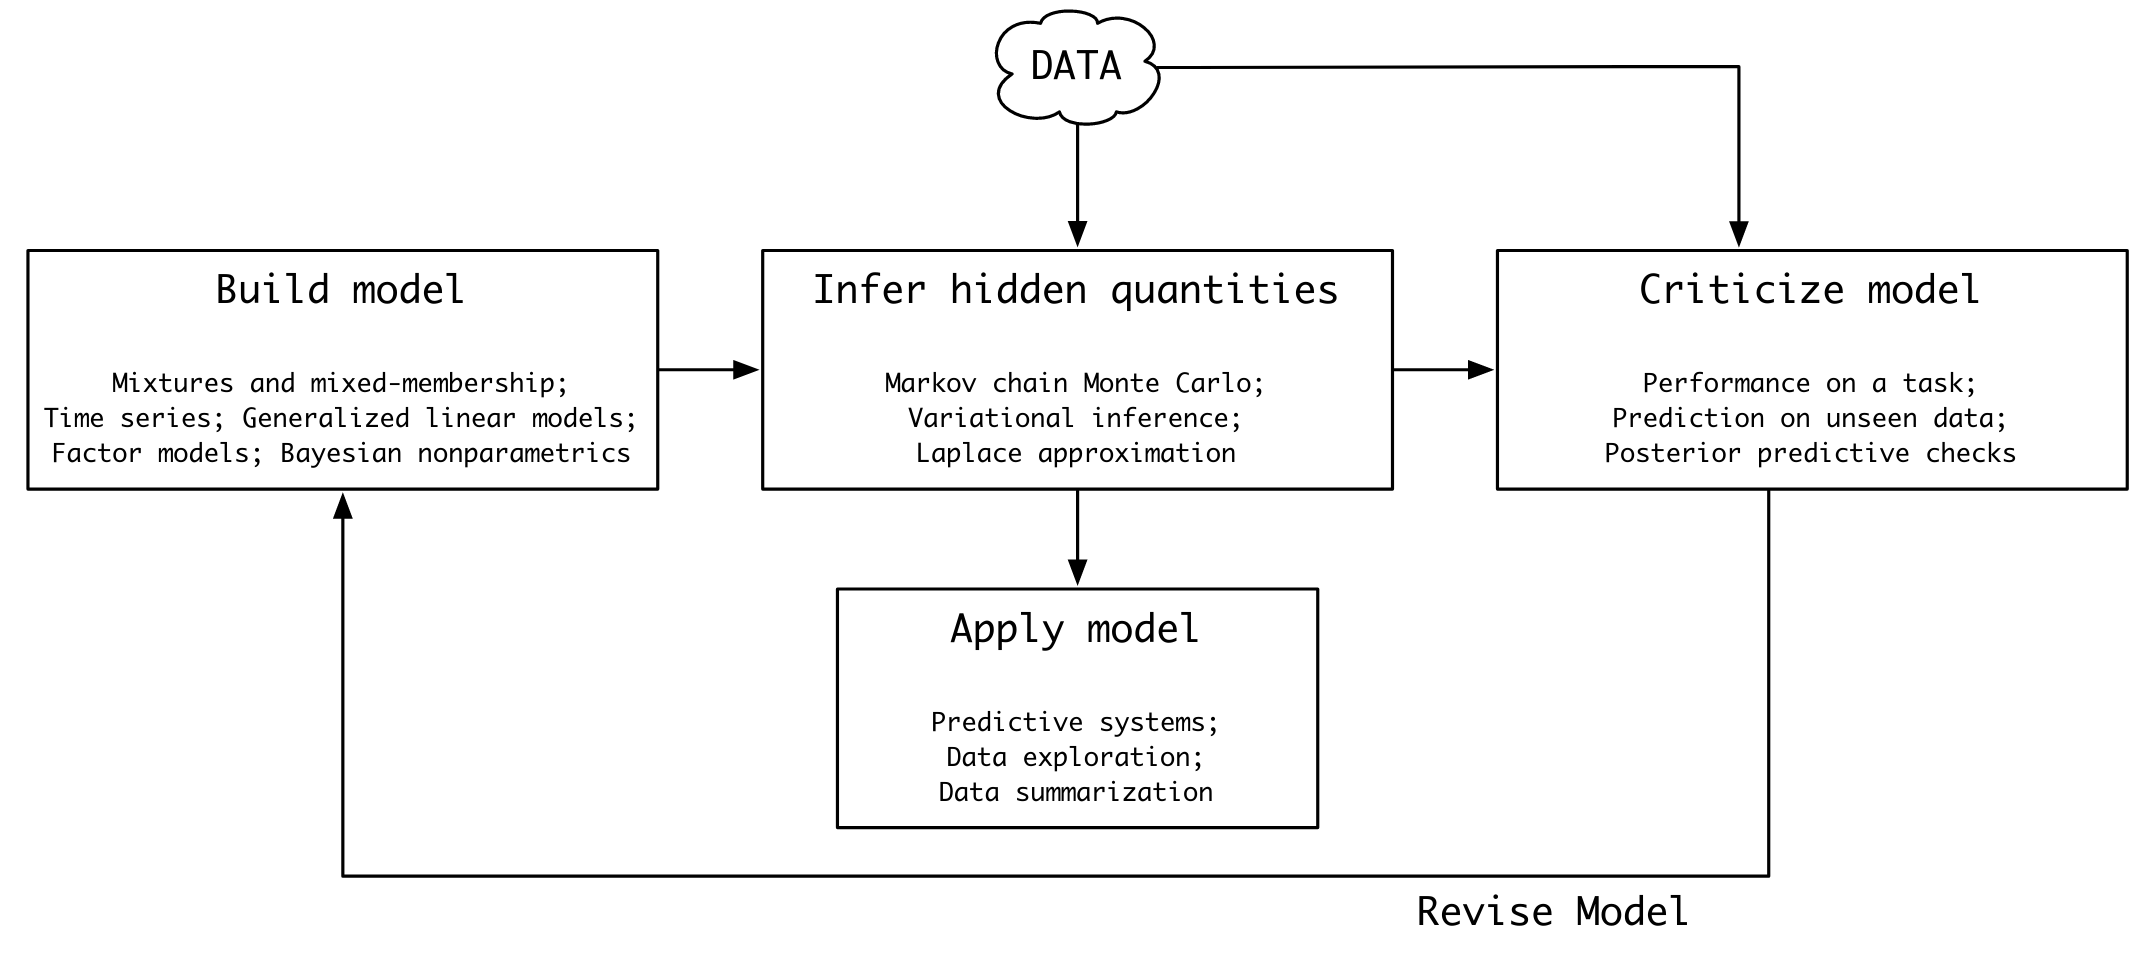
\includegraphics[width=0.8\textwidth]{box_loop.png}
		\caption{Box's Loop from \textcite{boxScienceStatistics1976}
			but taken from \textcite{Blei_Workflow2014}}
	\end{figure}
\end{frame}

\subsection{Prior Predictive Check}
\begin{frame}{Prior Predictive Check}
	Before we feed data into our model,
	we need to check all of our priors.
	\vfill
	In a very simple way, it consists in simulate parameter values based on
	prior distribution without conditioning on any data or employing any
	likelihood function.
	\vfill
	Independent of the level of information specified in the priors,
	it is always important to perform a prior sensitivity analysis
	in order to have a deep understanding of the prior influence onto
	the posterior.
\end{frame}

\subsection{Posterior Predictive Check}
\begin{frame}{Posterior Predictive Check}
	We need to make sure that the posterior distribution of $\mathbf{y}$,
	namely $\boldsymbol{\tilde{y}}$,
	can capture all the nuances of the real distribution density/mass of $\mathbf{y}$.
	\vfill
	This procedure is called \textbf{posterior predictive check},
	and it is generally carried on by a visual inspection\footnote{
		we also perform mathematical/exact inspections,
		see the section on \textit{Model Comparison}.}
	of the real density/mass of $\mathbf{y}$ against generated samples
	of $\mathbf{y}$ by the Bayesian model.
	\vfill
	The purpose is to compare the histogram of the dependent variable $\mathbf{y}$
	against the histograms of simulated dependent variables $\mathbf{y}_{\text{rep}}$
	by the model after parameter inference.\
	The ideia is that the real and simulated histograms blend together and
	we do not observer any divergences.
\end{frame}

\begin{frame}{Examples of Posterior Predictive Checks}
	% library(brms)
	% library(ggplot2)
	% library(ggdark)
	% library(bayesplot)
	% library(tikzDevice)
	% theme_set(dark_theme_light())
	% bayesplot_theme_set(dark_theme_light())
	% brms_fit <- brm(mpg ~ wt + am, data = mtcars)
	% tikz(file = "slides/images/pp_check_brms.tex")
	% pp_check(brms_fit, nreps = 10, seed = 123)
	% dev.off()
	% tikz(file = "slides/images/pp_check_brms_ecdf.tex")
	% pp_check(brms_fit, nreps = 10, seed = 123, type = "ecdf_overlay")
	% dev.off()
	\begin{columns}
		\begin{column}{0.5\textwidth}
			\begin{figure}
				\centering
				\resizebox{0.8\columnwidth}{!}{% Created by tikzDevice version 0.12.3.1 on 2021-06-01 06:51:26
% !TEX encoding = UTF-8 Unicode
\begin{tikzpicture}[x=1pt,y=1pt]
\definecolor{fillColor}{RGB}{255,255,255}
\path[use as bounding box,fill=fillColor,fill opacity=0.00] (0,0) rectangle (505.89,505.89);
\begin{scope}
\path[clip] (  0.00,  0.00) rectangle (505.89,505.89);
\definecolor{drawColor}{RGB}{0,0,0}
\definecolor{fillColor}{RGB}{0,0,0}

\path[draw=drawColor,line width= 0.6pt,line join=round,line cap=round,fill=fillColor] (  0.00,  0.00) rectangle (505.89,505.89);
\end{scope}
\begin{scope}
\path[clip] (  8.25, 18.22) rectangle (445.03,500.39);
\definecolor{fillColor}{RGB}{0,0,0}

\path[fill=fillColor] (  8.25, 18.22) rectangle (445.03,500.39);
\definecolor{drawColor}{gray}{0.13}

\path[draw=drawColor,line width= 0.1pt,line join=round] (  8.25, 73.33) --
	(445.03, 73.33);

\path[draw=drawColor,line width= 0.1pt,line join=round] (  8.25,183.56) --
	(445.03,183.56);

\path[draw=drawColor,line width= 0.1pt,line join=round] (  8.25,293.79) --
	(445.03,293.79);

\path[draw=drawColor,line width= 0.1pt,line join=round] (  8.25,404.01) --
	(445.03,404.01);

\path[draw=drawColor,line width= 0.1pt,line join=round] ( 49.12, 18.22) --
	( 49.12,500.39);

\path[draw=drawColor,line width= 0.1pt,line join=round] (174.24, 18.22) --
	(174.24,500.39);

\path[draw=drawColor,line width= 0.1pt,line join=round] (299.35, 18.22) --
	(299.35,500.39);

\path[draw=drawColor,line width= 0.1pt,line join=round] (424.47, 18.22) --
	(424.47,500.39);

\path[draw=drawColor,line width= 0.3pt,line join=round] (  8.25,128.45) --
	(445.03,128.45);

\path[draw=drawColor,line width= 0.3pt,line join=round] (  8.25,238.67) --
	(445.03,238.67);

\path[draw=drawColor,line width= 0.3pt,line join=round] (  8.25,348.90) --
	(445.03,348.90);

\path[draw=drawColor,line width= 0.3pt,line join=round] (  8.25,459.13) --
	(445.03,459.13);

\path[draw=drawColor,line width= 0.3pt,line join=round] (111.68, 18.22) --
	(111.68,500.39);

\path[draw=drawColor,line width= 0.3pt,line join=round] (236.80, 18.22) --
	(236.80,500.39);

\path[draw=drawColor,line width= 0.3pt,line join=round] (361.91, 18.22) --
	(361.91,500.39);
\definecolor{drawColor}{RGB}{179,205,224}

\path[draw=drawColor,draw opacity=0.70,line width= 0.3pt,line join=round] (  8.25, 18.31) --
	(  8.68, 18.32) --
	(  9.10, 18.33) --
	(  9.53, 18.33) --
	(  9.96, 18.34) --
	( 10.38, 18.35) --
	( 10.81, 18.35) --
	( 11.24, 18.36) --
	( 11.67, 18.37) --
	( 12.09, 18.38) --
	( 12.52, 18.39) --
	( 12.95, 18.40) --
	( 13.37, 18.41) --
	( 13.80, 18.42) --
	( 14.23, 18.43) --
	( 14.65, 18.44) --
	( 15.08, 18.46) --
	( 15.51, 18.47) --
	( 15.94, 18.49) --
	( 16.36, 18.50) --
	( 16.79, 18.52) --
	( 17.22, 18.53) --
	( 17.64, 18.55) --
	( 18.07, 18.57) --
	( 18.50, 18.59) --
	( 18.92, 18.61) --
	( 19.35, 18.63) --
	( 19.78, 18.65) --
	( 20.20, 18.68) --
	( 20.63, 18.70) --
	( 21.06, 18.73) --
	( 21.49, 18.76) --
	( 21.91, 18.79) --
	( 22.34, 18.82) --
	( 22.77, 18.85) --
	( 23.19, 18.88) --
	( 23.62, 18.91) --
	( 24.05, 18.95) --
	( 24.47, 18.99) --
	( 24.90, 19.03) --
	( 25.33, 19.07) --
	( 25.76, 19.11) --
	( 26.18, 19.16) --
	( 26.61, 19.20) --
	( 27.04, 19.25) --
	( 27.46, 19.30) --
	( 27.89, 19.36) --
	( 28.32, 19.41) --
	( 28.74, 19.47) --
	( 29.17, 19.53) --
	( 29.60, 19.59) --
	( 30.02, 19.66) --
	( 30.45, 19.72) --
	( 30.88, 19.79) --
	( 31.31, 19.87) --
	( 31.73, 19.94) --
	( 32.16, 20.02) --
	( 32.59, 20.11) --
	( 33.01, 20.19) --
	( 33.44, 20.28) --
	( 33.87, 20.37) --
	( 34.29, 20.47) --
	( 34.72, 20.57) --
	( 35.15, 20.67) --
	( 35.58, 20.78) --
	( 36.00, 20.89) --
	( 36.43, 21.00) --
	( 36.86, 21.12) --
	( 37.28, 21.25) --
	( 37.71, 21.37) --
	( 38.14, 21.50) --
	( 38.56, 21.64) --
	( 38.99, 21.78) --
	( 39.42, 21.93) --
	( 39.84, 22.08) --
	( 40.27, 22.23) --
	( 40.70, 22.39) --
	( 41.13, 22.56) --
	( 41.55, 22.73) --
	( 41.98, 22.91) --
	( 42.41, 23.09) --
	( 42.83, 23.28) --
	( 43.26, 23.47) --
	( 43.69, 23.67) --
	( 44.11, 23.87) --
	( 44.54, 24.08) --
	( 44.97, 24.30) --
	( 45.40, 24.52) --
	( 45.82, 24.75) --
	( 46.25, 24.99) --
	( 46.68, 25.23) --
	( 47.10, 25.48) --
	( 47.53, 25.74) --
	( 47.96, 26.00) --
	( 48.38, 26.27) --
	( 48.81, 26.54) --
	( 49.24, 26.83) --
	( 49.66, 27.12) --
	( 50.09, 27.42) --
	( 50.52, 27.72) --
	( 50.95, 28.03) --
	( 51.37, 28.35) --
	( 51.80, 28.68) --
	( 52.23, 29.02) --
	( 52.65, 29.36) --
	( 53.08, 29.71) --
	( 53.51, 30.07) --
	( 53.93, 30.43) --
	( 54.36, 30.81) --
	( 54.79, 31.19) --
	( 55.22, 31.58) --
	( 55.64, 31.97) --
	( 56.07, 32.38) --
	( 56.50, 32.79) --
	( 56.92, 33.21) --
	( 57.35, 33.64) --
	( 57.78, 34.07) --
	( 58.20, 34.52) --
	( 58.63, 34.97) --
	( 59.06, 35.43) --
	( 59.48, 35.90) --
	( 59.91, 36.37) --
	( 60.34, 36.85) --
	( 60.77, 37.34) --
	( 61.19, 37.84) --
	( 61.62, 38.34) --
	( 62.05, 38.86) --
	( 62.47, 39.37) --
	( 62.90, 39.90) --
	( 63.33, 40.43) --
	( 63.75, 40.97) --
	( 64.18, 41.52) --
	( 64.61, 42.07) --
	( 65.04, 42.63) --
	( 65.46, 43.20) --
	( 65.89, 43.77) --
	( 66.32, 44.35) --
	( 66.74, 44.93) --
	( 67.17, 45.52) --
	( 67.60, 46.12) --
	( 68.02, 46.72) --
	( 68.45, 47.32) --
	( 68.88, 47.93) --
	( 69.30, 48.55) --
	( 69.73, 49.17) --
	( 70.16, 49.79) --
	( 70.59, 50.42) --
	( 71.01, 51.05) --
	( 71.44, 51.68) --
	( 71.87, 52.32) --
	( 72.29, 52.96) --
	( 72.72, 53.61) --
	( 73.15, 54.25) --
	( 73.57, 54.90) --
	( 74.00, 55.55) --
	( 74.43, 56.20) --
	( 74.86, 56.85) --
	( 75.28, 57.50) --
	( 75.71, 58.15) --
	( 76.14, 58.81) --
	( 76.56, 59.46) --
	( 76.99, 60.11) --
	( 77.42, 60.76) --
	( 77.84, 61.41) --
	( 78.27, 62.06) --
	( 78.70, 62.71) --
	( 79.12, 63.35) --
	( 79.55, 64.00) --
	( 79.98, 64.64) --
	( 80.41, 65.27) --
	( 80.83, 65.91) --
	( 81.26, 66.53) --
	( 81.69, 67.16) --
	( 82.11, 67.78) --
	( 82.54, 68.39) --
	( 82.97, 69.00) --
	( 83.39, 69.60) --
	( 83.82, 70.20) --
	( 84.25, 70.79) --
	( 84.68, 71.38) --
	( 85.10, 71.96) --
	( 85.53, 72.53) --
	( 85.96, 73.09) --
	( 86.38, 73.64) --
	( 86.81, 74.19) --
	( 87.24, 74.73) --
	( 87.66, 75.26) --
	( 88.09, 75.78) --
	( 88.52, 76.29) --
	( 88.94, 76.79) --
	( 89.37, 77.28) --
	( 89.80, 77.76) --
	( 90.23, 78.22) --
	( 90.65, 78.68) --
	( 91.08, 79.13) --
	( 91.51, 79.57) --
	( 91.93, 79.99) --
	( 92.36, 80.40) --
	( 92.79, 80.80) --
	( 93.21, 81.19) --
	( 93.64, 81.57) --
	( 94.07, 81.93) --
	( 94.49, 82.28) --
	( 94.92, 82.62) --
	( 95.35, 82.95) --
	( 95.78, 83.26) --
	( 96.20, 83.56) --
	( 96.63, 83.85) --
	( 97.06, 84.12) --
	( 97.48, 84.38) --
	( 97.91, 84.63) --
	( 98.34, 84.86) --
	( 98.76, 85.08) --
	( 99.19, 85.29) --
	( 99.62, 85.48) --
	(100.05, 85.66) --
	(100.47, 85.83) --
	(100.90, 85.98) --
	(101.33, 86.12) --
	(101.75, 86.25) --
	(102.18, 86.36) --
	(102.61, 86.46) --
	(103.03, 86.55) --
	(103.46, 86.63) --
	(103.89, 86.69) --
	(104.31, 86.74) --
	(104.74, 86.78) --
	(105.17, 86.80) --
	(105.60, 86.82) --
	(106.02, 86.83) --
	(106.45, 86.82) --
	(106.88, 86.80) --
	(107.30, 86.77) --
	(107.73, 86.73) --
	(108.16, 86.69) --
	(108.58, 86.63) --
	(109.01, 86.56) --
	(109.44, 86.48) --
	(109.87, 86.40) --
	(110.29, 86.31) --
	(110.72, 86.20) --
	(111.15, 86.09) --
	(111.57, 85.98) --
	(112.00, 85.86) --
	(112.43, 85.73) --
	(112.85, 85.59) --
	(113.28, 85.45) --
	(113.71, 85.30) --
	(114.13, 85.15) --
	(114.56, 85.00) --
	(114.99, 84.84) --
	(115.42, 84.68) --
	(115.84, 84.52) --
	(116.27, 84.35) --
	(116.70, 84.18) --
	(117.12, 84.01) --
	(117.55, 83.84) --
	(117.98, 83.67) --
	(118.40, 83.50) --
	(118.83, 83.33) --
	(119.26, 83.16) --
	(119.69, 82.99) --
	(120.11, 82.83) --
	(120.54, 82.67) --
	(120.97, 82.51) --
	(121.39, 82.35) --
	(121.82, 82.20) --
	(122.25, 82.05) --
	(122.67, 81.91) --
	(123.10, 81.77) --
	(123.53, 81.64) --
	(123.95, 81.51) --
	(124.38, 81.40) --
	(124.81, 81.29) --
	(125.24, 81.18) --
	(125.66, 81.09) --
	(126.09, 81.00) --
	(126.52, 80.93) --
	(126.94, 80.86) --
	(127.37, 80.80) --
	(127.80, 80.76) --
	(128.22, 80.72) --
	(128.65, 80.70) --
	(129.08, 80.68) --
	(129.51, 80.68) --
	(129.93, 80.69) --
	(130.36, 80.72) --
	(130.79, 80.75) --
	(131.21, 80.80) --
	(131.64, 80.87) --
	(132.07, 80.94) --
	(132.49, 81.03) --
	(132.92, 81.14) --
	(133.35, 81.26) --
	(133.77, 81.39) --
	(134.20, 81.55) --
	(134.63, 81.71) --
	(135.06, 81.89) --
	(135.48, 82.09) --
	(135.91, 82.31) --
	(136.34, 82.54) --
	(136.76, 82.79) --
	(137.19, 83.05) --
	(137.62, 83.33) --
	(138.04, 83.63) --
	(138.47, 83.95) --
	(138.90, 84.28) --
	(139.33, 84.62) --
	(139.75, 84.99) --
	(140.18, 85.38) --
	(140.61, 85.78) --
	(141.03, 86.20) --
	(141.46, 86.64) --
	(141.89, 87.10) --
	(142.31, 87.57) --
	(142.74, 88.06) --
	(143.17, 88.57) --
	(143.59, 89.10) --
	(144.02, 89.65) --
	(144.45, 90.21) --
	(144.88, 90.79) --
	(145.30, 91.40) --
	(145.73, 92.02) --
	(146.16, 92.65) --
	(146.58, 93.31) --
	(147.01, 93.99) --
	(147.44, 94.68) --
	(147.86, 95.39) --
	(148.29, 96.12) --
	(148.72, 96.86) --
	(149.15, 97.63) --
	(149.57, 98.41) --
	(150.00, 99.21) --
	(150.43,100.03) --
	(150.85,100.87) --
	(151.28,101.73) --
	(151.71,102.60) --
	(152.13,103.49) --
	(152.56,104.40) --
	(152.99,105.33) --
	(153.41,106.27) --
	(153.84,107.24) --
	(154.27,108.22) --
	(154.70,109.22) --
	(155.12,110.24) --
	(155.55,111.28) --
	(155.98,112.33) --
	(156.40,113.41) --
	(156.83,114.50) --
	(157.26,115.60) --
	(157.68,116.74) --
	(158.11,117.88) --
	(158.54,119.05) --
	(158.97,120.23) --
	(159.39,121.43) --
	(159.82,122.65) --
	(160.25,123.89) --
	(160.67,125.16) --
	(161.10,126.43) --
	(161.53,127.73) --
	(161.95,129.05) --
	(162.38,130.38) --
	(162.81,131.74) --
	(163.23,133.12) --
	(163.66,134.51) --
	(164.09,135.93) --
	(164.52,137.36) --
	(164.94,138.82) --
	(165.37,140.30) --
	(165.80,141.79) --
	(166.22,143.32) --
	(166.65,144.85) --
	(167.08,146.41) --
	(167.50,148.00) --
	(167.93,149.61) --
	(168.36,151.23) --
	(168.79,152.88) --
	(169.21,154.55) --
	(169.64,156.25) --
	(170.07,157.96) --
	(170.49,159.71) --
	(170.92,161.47) --
	(171.35,163.26) --
	(171.77,165.07) --
	(172.20,166.90) --
	(172.63,168.76) --
	(173.05,170.65) --
	(173.48,172.56) --
	(173.91,174.49) --
	(174.34,176.45) --
	(174.76,178.43) --
	(175.19,180.44) --
	(175.62,182.47) --
	(176.04,184.54) --
	(176.47,186.62) --
	(176.90,188.73) --
	(177.32,190.87) --
	(177.75,193.03) --
	(178.18,195.22) --
	(178.61,197.44) --
	(179.03,199.68) --
	(179.46,201.95) --
	(179.89,204.25) --
	(180.31,206.57) --
	(180.74,208.92) --
	(181.17,211.30) --
	(181.59,213.70) --
	(182.02,216.13) --
	(182.45,218.58) --
	(182.87,221.07) --
	(183.30,223.57) --
	(183.73,226.10) --
	(184.16,228.67) --
	(184.58,231.25) --
	(185.01,233.86) --
	(185.44,236.50) --
	(185.86,239.16) --
	(186.29,241.84) --
	(186.72,244.55) --
	(187.14,247.29) --
	(187.57,250.05) --
	(188.00,252.83) --
	(188.43,255.64) --
	(188.85,258.46) --
	(189.28,261.31) --
	(189.71,264.18) --
	(190.13,267.08) --
	(190.56,269.98) --
	(190.99,272.92) --
	(191.41,275.87) --
	(191.84,278.84) --
	(192.27,281.83) --
	(192.69,284.84) --
	(193.12,287.86) --
	(193.55,290.90) --
	(193.98,293.96) --
	(194.40,297.03) --
	(194.83,300.11) --
	(195.26,303.21) --
	(195.68,306.32) --
	(196.11,309.43) --
	(196.54,312.57) --
	(196.96,315.70) --
	(197.39,318.85) --
	(197.82,322.01) --
	(198.25,325.17) --
	(198.67,328.33) --
	(199.10,331.51) --
	(199.53,334.68) --
	(199.95,337.86) --
	(200.38,341.04) --
	(200.81,344.21) --
	(201.23,347.39) --
	(201.66,350.57) --
	(202.09,353.74) --
	(202.51,356.91) --
	(202.94,360.07) --
	(203.37,363.22) --
	(203.80,366.37) --
	(204.22,369.51) --
	(204.65,372.64) --
	(205.08,375.75) --
	(205.50,378.85) --
	(205.93,381.95) --
	(206.36,385.02) --
	(206.78,388.07) --
	(207.21,391.12) --
	(207.64,394.13) --
	(208.07,397.13) --
	(208.49,400.11) --
	(208.92,403.07) --
	(209.35,406.00) --
	(209.77,408.91) --
	(210.20,411.79) --
	(210.63,414.63) --
	(211.05,417.46) --
	(211.48,420.26) --
	(211.91,423.01) --
	(212.33,425.74) --
	(212.76,428.44) --
	(213.19,431.10) --
	(213.62,433.72) --
	(214.04,436.31) --
	(214.47,438.86) --
	(214.90,441.37) --
	(215.32,443.84) --
	(215.75,446.27) --
	(216.18,448.65) --
	(216.60,450.99) --
	(217.03,453.30) --
	(217.46,455.54) --
	(217.89,457.74) --
	(218.31,459.91) --
	(218.74,462.01) --
	(219.17,464.07) --
	(219.59,466.09) --
	(220.02,468.04) --
	(220.45,469.94) --
	(220.87,471.80) --
	(221.30,473.60) --
	(221.73,475.34) --
	(222.15,477.04) --
	(222.58,478.68) --
	(223.01,480.25) --
	(223.44,481.78) --
	(223.86,483.25) --
	(224.29,484.65) --
	(224.72,486.00) --
	(225.14,487.30) --
	(225.57,488.53) --
	(226.00,489.69) --
	(226.42,490.81) --
	(226.85,491.87) --
	(227.28,492.85) --
	(227.71,493.79) --
	(228.13,494.66) --
	(228.56,495.46) --
	(228.99,496.21) --
	(229.41,496.91) --
	(229.84,497.52) --
	(230.27,498.08) --
	(230.69,498.60) --
	(231.12,499.03) --
	(231.55,499.40) --
	(231.97,499.73) --
	(232.40,499.98) --
	(232.83,500.17) --
	(233.26,500.31) --
	(233.68,500.39) --
	(234.11,500.39) --
	(234.54,500.34) --
	(234.96,500.25) --
	(235.39,500.07) --
	(235.82,499.85) --
	(236.24,499.58) --
	(236.67,499.23) --
	(237.10,498.83) --
	(237.53,498.38) --
	(237.95,497.87) --
	(238.38,497.30) --
	(238.81,496.68) --
	(239.23,496.01) --
	(239.66,495.28) --
	(240.09,494.50) --
	(240.51,493.68) --
	(240.94,492.79) --
	(241.37,491.86) --
	(241.79,490.89) --
	(242.22,489.85) --
	(242.65,488.77) --
	(243.08,487.66) --
	(243.50,486.49) --
	(243.93,485.28) --
	(244.36,484.03) --
	(244.78,482.74) --
	(245.21,481.39) --
	(245.64,480.02) --
	(246.06,478.61) --
	(246.49,477.16) --
	(246.92,475.67) --
	(247.35,474.15) --
	(247.77,472.59) --
	(248.20,471.00) --
	(248.63,469.39) --
	(249.05,467.74) --
	(249.48,466.06) --
	(249.91,464.35) --
	(250.33,462.62) --
	(250.76,460.86) --
	(251.19,459.09) --
	(251.61,457.29) --
	(252.04,455.46) --
	(252.47,453.62) --
	(252.90,451.76) --
	(253.32,449.88) --
	(253.75,447.99) --
	(254.18,446.08) --
	(254.60,444.16) --
	(255.03,442.23) --
	(255.46,440.28) --
	(255.88,438.33) --
	(256.31,436.37) --
	(256.74,434.40) --
	(257.17,432.43) --
	(257.59,430.46) --
	(258.02,428.48) --
	(258.45,426.50) --
	(258.87,424.52) --
	(259.30,422.54) --
	(259.73,420.56) --
	(260.15,418.58) --
	(260.58,416.61) --
	(261.01,414.64) --
	(261.43,412.68) --
	(261.86,410.73) --
	(262.29,408.78) --
	(262.72,406.85) --
	(263.14,404.92) --
	(263.57,403.01) --
	(264.00,401.10) --
	(264.42,399.22) --
	(264.85,397.34) --
	(265.28,395.48) --
	(265.70,393.63) --
	(266.13,391.80) --
	(266.56,389.99) --
	(266.98,388.19) --
	(267.41,386.41) --
	(267.84,384.65) --
	(268.27,382.91) --
	(268.69,381.19) --
	(269.12,379.49) --
	(269.55,377.81) --
	(269.97,376.15) --
	(270.40,374.51) --
	(270.83,372.89) --
	(271.25,371.30) --
	(271.68,369.73) --
	(272.11,368.18) --
	(272.54,366.65) --
	(272.96,365.15) --
	(273.39,363.67) --
	(273.82,362.20) --
	(274.24,360.77) --
	(274.67,359.36) --
	(275.10,357.97) --
	(275.52,356.61) --
	(275.95,355.26) --
	(276.38,353.94) --
	(276.80,352.64) --
	(277.23,351.37) --
	(277.66,350.12) --
	(278.09,348.88) --
	(278.51,347.68) --
	(278.94,346.49) --
	(279.37,345.32) --
	(279.79,344.17) --
	(280.22,343.05) --
	(280.65,341.94) --
	(281.07,340.85) --
	(281.50,339.79) --
	(281.93,338.74) --
	(282.36,337.71) --
	(282.78,336.69) --
	(283.21,335.69) --
	(283.64,334.71) --
	(284.06,333.75) --
	(284.49,332.80) --
	(284.92,331.86) --
	(285.34,330.94) --
	(285.77,330.04) --
	(286.20,329.14) --
	(286.62,328.26) --
	(287.05,327.39) --
	(287.48,326.52) --
	(287.91,325.67) --
	(288.33,324.83) --
	(288.76,324.00) --
	(289.19,323.17) --
	(289.61,322.36) --
	(290.04,321.55) --
	(290.47,320.74) --
	(290.89,319.94) --
	(291.32,319.14) --
	(291.75,318.35) --
	(292.18,317.56) --
	(292.60,316.78) --
	(293.03,315.99) --
	(293.46,315.21) --
	(293.88,314.42) --
	(294.31,313.64) --
	(294.74,312.85) --
	(295.16,312.06) --
	(295.59,311.27) --
	(296.02,310.48) --
	(296.44,309.68) --
	(296.87,308.88) --
	(297.30,308.08) --
	(297.73,307.27) --
	(298.15,306.45) --
	(298.58,305.63) --
	(299.01,304.79) --
	(299.43,303.95) --
	(299.86,303.11) --
	(300.29,302.25) --
	(300.71,301.39) --
	(301.14,300.51) --
	(301.57,299.63) --
	(302.00,298.73) --
	(302.42,297.82) --
	(302.85,296.91) --
	(303.28,295.98) --
	(303.70,295.03) --
	(304.13,294.08) --
	(304.56,293.11) --
	(304.98,292.13) --
	(305.41,291.13) --
	(305.84,290.12) --
	(306.26,289.10) --
	(306.69,288.06) --
	(307.12,287.01) --
	(307.55,285.94) --
	(307.97,284.86) --
	(308.40,283.76) --
	(308.83,282.65) --
	(309.25,281.52) --
	(309.68,280.37) --
	(310.11,279.21) --
	(310.53,278.03) --
	(310.96,276.84) --
	(311.39,275.63) --
	(311.82,274.41) --
	(312.24,273.16) --
	(312.67,271.91) --
	(313.10,270.63) --
	(313.52,269.34) --
	(313.95,268.04) --
	(314.38,266.71) --
	(314.80,265.38) --
	(315.23,264.02) --
	(315.66,262.65) --
	(316.08,261.27) --
	(316.51,259.87) --
	(316.94,258.45) --
	(317.37,257.02) --
	(317.79,255.57) --
	(318.22,254.11) --
	(318.65,252.64) --
	(319.07,251.15) --
	(319.50,249.65) --
	(319.93,248.13) --
	(320.35,246.60) --
	(320.78,245.05) --
	(321.21,243.50) --
	(321.64,241.93) --
	(322.06,240.35) --
	(322.49,238.75) --
	(322.92,237.15) --
	(323.34,235.53) --
	(323.77,233.91) --
	(324.20,232.27) --
	(324.62,230.62) --
	(325.05,228.97) --
	(325.48,227.30) --
	(325.90,225.63) --
	(326.33,223.94) --
	(326.76,222.25) --
	(327.19,220.56) --
	(327.61,218.85) --
	(328.04,217.14) --
	(328.47,215.42) --
	(328.89,213.70) --
	(329.32,211.97) --
	(329.75,210.24) --
	(330.17,208.50) --
	(330.60,206.76) --
	(331.03,205.02) --
	(331.46,203.28) --
	(331.88,201.53) --
	(332.31,199.78) --
	(332.74,198.03) --
	(333.16,196.28) --
	(333.59,194.52) --
	(334.02,192.77) --
	(334.44,191.02) --
	(334.87,189.27) --
	(335.30,187.53) --
	(335.72,185.78) --
	(336.15,184.04) --
	(336.58,182.30) --
	(337.01,180.56) --
	(337.43,178.83) --
	(337.86,177.10) --
	(338.29,175.38) --
	(338.71,173.67) --
	(339.14,171.95) --
	(339.57,170.25) --
	(339.99,168.55) --
	(340.42,166.86) --
	(340.85,165.18) --
	(341.28,163.50) --
	(341.70,161.84) --
	(342.13,160.18) --
	(342.56,158.53) --
	(342.98,156.89) --
	(343.41,155.26) --
	(343.84,153.64) --
	(344.26,152.03) --
	(344.69,150.43) --
	(345.12,148.85) --
	(345.54,147.27) --
	(345.97,145.70) --
	(346.40,144.15) --
	(346.83,142.61) --
	(347.25,141.08) --
	(347.68,139.57) --
	(348.11,138.06) --
	(348.53,136.57) --
	(348.96,135.09) --
	(349.39,133.63) --
	(349.81,132.18) --
	(350.24,130.74) --
	(350.67,129.32) --
	(351.10,127.91) --
	(351.52,126.51) --
	(351.95,125.13) --
	(352.38,123.76) --
	(352.80,122.40) --
	(353.23,121.06) --
	(353.66,119.74) --
	(354.08,118.42) --
	(354.51,117.12) --
	(354.94,115.84) --
	(355.36,114.57) --
	(355.79,113.31) --
	(356.22,112.07) --
	(356.65,110.84) --
	(357.07,109.63) --
	(357.50,108.43) --
	(357.93,107.25) --
	(358.35,106.07) --
	(358.78,104.92) --
	(359.21,103.77) --
	(359.63,102.64) --
	(360.06,101.52) --
	(360.49,100.42) --
	(360.92, 99.33) --
	(361.34, 98.25) --
	(361.77, 97.19) --
	(362.20, 96.13) --
	(362.62, 95.09) --
	(363.05, 94.07) --
	(363.48, 93.05) --
	(363.90, 92.05) --
	(364.33, 91.06) --
	(364.76, 90.09) --
	(365.18, 89.12) --
	(365.61, 88.17) --
	(366.04, 87.23) --
	(366.47, 86.30) --
	(366.89, 85.38) --
	(367.32, 84.47) --
	(367.75, 83.58) --
	(368.17, 82.69) --
	(368.60, 81.82) --
	(369.03, 80.96) --
	(369.45, 80.10) --
	(369.88, 79.26) --
	(370.31, 78.43) --
	(370.74, 77.61) --
	(371.16, 76.80) --
	(371.59, 76.00) --
	(372.02, 75.21) --
	(372.44, 74.43) --
	(372.87, 73.66) --
	(373.30, 72.90) --
	(373.72, 72.15) --
	(374.15, 71.41) --
	(374.58, 70.68) --
	(375.00, 69.95) --
	(375.43, 69.24) --
	(375.86, 68.54) --
	(376.29, 67.84) --
	(376.71, 67.16) --
	(377.14, 66.49) --
	(377.57, 65.82) --
	(377.99, 65.16) --
	(378.42, 64.52) --
	(378.85, 63.88) --
	(379.27, 63.25) --
	(379.70, 62.63) --
	(380.13, 62.02) --
	(380.56, 61.42) --
	(380.98, 60.83) --
	(381.41, 60.25) --
	(381.84, 59.68) --
	(382.26, 59.12) --
	(382.69, 58.56) --
	(383.12, 58.02) --
	(383.54, 57.48) --
	(383.97, 56.96) --
	(384.40, 56.45) --
	(384.82, 55.94) --
	(385.25, 55.45) --
	(385.68, 54.96) --
	(386.11, 54.48) --
	(386.53, 54.02) --
	(386.96, 53.57) --
	(387.39, 53.12) --
	(387.81, 52.69) --
	(388.24, 52.26) --
	(388.67, 51.85) --
	(389.09, 51.45) --
	(389.52, 51.05) --
	(389.95, 50.67) --
	(390.38, 50.30) --
	(390.80, 49.94) --
	(391.23, 49.59) --
	(391.66, 49.25) --
	(392.08, 48.93) --
	(392.51, 48.61) --
	(392.94, 48.30) --
	(393.36, 48.01) --
	(393.79, 47.73) --
	(394.22, 47.45) --
	(394.64, 47.19) --
	(395.07, 46.94) --
	(395.50, 46.70) --
	(395.93, 46.48) --
	(396.35, 46.26) --
	(396.78, 46.06) --
	(397.21, 45.87) --
	(397.63, 45.69) --
	(398.06, 45.52) --
	(398.49, 45.36) --
	(398.91, 45.21) --
	(399.34, 45.08) --
	(399.77, 44.95) --
	(400.20, 44.84) --
	(400.62, 44.74) --
	(401.05, 44.64) --
	(401.48, 44.56) --
	(401.90, 44.50) --
	(402.33, 44.44) --
	(402.76, 44.39) --
	(403.18, 44.35) --
	(403.61, 44.33) --
	(404.04, 44.31) --
	(404.46, 44.31) --
	(404.89, 44.31) --
	(405.32, 44.32) --
	(405.75, 44.35) --
	(406.17, 44.38) --
	(406.60, 44.43) --
	(407.03, 44.48) --
	(407.45, 44.54) --
	(407.88, 44.61) --
	(408.31, 44.69) --
	(408.73, 44.78) --
	(409.16, 44.88) --
	(409.59, 44.98) --
	(410.02, 45.09) --
	(410.44, 45.21) --
	(410.87, 45.34) --
	(411.30, 45.47) --
	(411.72, 45.61) --
	(412.15, 45.76) --
	(412.58, 45.91) --
	(413.00, 46.07) --
	(413.43, 46.23) --
	(413.86, 46.40) --
	(414.28, 46.58) --
	(414.71, 46.76) --
	(415.14, 46.94) --
	(415.57, 47.13) --
	(415.99, 47.32) --
	(416.42, 47.51) --
	(416.85, 47.71) --
	(417.27, 47.91) --
	(417.70, 48.11) --
	(418.13, 48.31) --
	(418.55, 48.52) --
	(418.98, 48.72) --
	(419.41, 48.93) --
	(419.84, 49.14) --
	(420.26, 49.34) --
	(420.69, 49.55) --
	(421.12, 49.76) --
	(421.54, 49.96) --
	(421.97, 50.17) --
	(422.40, 50.37) --
	(422.82, 50.57) --
	(423.25, 50.77) --
	(423.68, 50.97) --
	(424.10, 51.16) --
	(424.53, 51.35) --
	(424.96, 51.54) --
	(425.39, 51.72) --
	(425.81, 51.90) --
	(426.24, 52.07) --
	(426.67, 52.24) --
	(427.09, 52.40) --
	(427.52, 52.56) --
	(427.95, 52.71) --
	(428.37, 52.86) --
	(428.80, 53.00) --
	(429.23, 53.14) --
	(429.66, 53.26) --
	(430.08, 53.38) --
	(430.51, 53.50) --
	(430.94, 53.60) --
	(431.36, 53.70) --
	(431.79, 53.79) --
	(432.22, 53.87) --
	(432.64, 53.94) --
	(433.07, 54.01) --
	(433.50, 54.07) --
	(433.92, 54.11) --
	(434.35, 54.15) --
	(434.78, 54.18) --
	(435.21, 54.20) --
	(435.63, 54.22) --
	(436.06, 54.22) --
	(436.49, 54.21) --
	(436.91, 54.20) --
	(437.34, 54.17) --
	(437.77, 54.13) --
	(438.19, 54.09) --
	(438.62, 54.04) --
	(439.05, 53.97) --
	(439.47, 53.89) --
	(439.90, 53.81) --
	(440.33, 53.72) --
	(440.76, 53.61) --
	(441.18, 53.50) --
	(441.61, 53.38) --
	(442.04, 53.25) --
	(442.46, 53.10) --
	(442.89, 52.96) --
	(443.32, 52.79) --
	(443.74, 52.62) --
	(444.17, 52.45) --
	(444.60, 52.26) --
	(445.03, 52.06);

\path[draw=drawColor,draw opacity=0.70,line width= 0.3pt,line join=round] (  8.25, 19.19) --
	(  8.68, 19.23) --
	(  9.10, 19.26) --
	(  9.53, 19.30) --
	(  9.96, 19.34) --
	( 10.38, 19.38) --
	( 10.81, 19.42) --
	( 11.24, 19.47) --
	( 11.67, 19.51) --
	( 12.09, 19.56) --
	( 12.52, 19.61) --
	( 12.95, 19.66) --
	( 13.37, 19.71) --
	( 13.80, 19.76) --
	( 14.23, 19.82) --
	( 14.65, 19.87) --
	( 15.08, 19.93) --
	( 15.51, 19.99) --
	( 15.94, 20.05) --
	( 16.36, 20.11) --
	( 16.79, 20.18) --
	( 17.22, 20.24) --
	( 17.64, 20.31) --
	( 18.07, 20.38) --
	( 18.50, 20.45) --
	( 18.92, 20.53) --
	( 19.35, 20.60) --
	( 19.78, 20.68) --
	( 20.20, 20.76) --
	( 20.63, 20.85) --
	( 21.06, 20.93) --
	( 21.49, 21.02) --
	( 21.91, 21.11) --
	( 22.34, 21.20) --
	( 22.77, 21.30) --
	( 23.19, 21.39) --
	( 23.62, 21.49) --
	( 24.05, 21.60) --
	( 24.47, 21.70) --
	( 24.90, 21.81) --
	( 25.33, 21.92) --
	( 25.76, 22.03) --
	( 26.18, 22.15) --
	( 26.61, 22.27) --
	( 27.04, 22.39) --
	( 27.46, 22.52) --
	( 27.89, 22.64) --
	( 28.32, 22.77) --
	( 28.74, 22.91) --
	( 29.17, 23.05) --
	( 29.60, 23.19) --
	( 30.02, 23.33) --
	( 30.45, 23.48) --
	( 30.88, 23.63) --
	( 31.31, 23.79) --
	( 31.73, 23.94) --
	( 32.16, 24.10) --
	( 32.59, 24.27) --
	( 33.01, 24.44) --
	( 33.44, 24.61) --
	( 33.87, 24.79) --
	( 34.29, 24.97) --
	( 34.72, 25.15) --
	( 35.15, 25.34) --
	( 35.58, 25.53) --
	( 36.00, 25.73) --
	( 36.43, 25.93) --
	( 36.86, 26.13) --
	( 37.28, 26.34) --
	( 37.71, 26.55) --
	( 38.14, 26.77) --
	( 38.56, 26.99) --
	( 38.99, 27.22) --
	( 39.42, 27.45) --
	( 39.84, 27.68) --
	( 40.27, 27.92) --
	( 40.70, 28.17) --
	( 41.13, 28.42) --
	( 41.55, 28.67) --
	( 41.98, 28.93) --
	( 42.41, 29.19) --
	( 42.83, 29.46) --
	( 43.26, 29.73) --
	( 43.69, 30.01) --
	( 44.11, 30.29) --
	( 44.54, 30.58) --
	( 44.97, 30.87) --
	( 45.40, 31.17) --
	( 45.82, 31.47) --
	( 46.25, 31.78) --
	( 46.68, 32.09) --
	( 47.10, 32.41) --
	( 47.53, 32.73) --
	( 47.96, 33.06) --
	( 48.38, 33.40) --
	( 48.81, 33.74) --
	( 49.24, 34.08) --
	( 49.66, 34.43) --
	( 50.09, 34.79) --
	( 50.52, 35.15) --
	( 50.95, 35.52) --
	( 51.37, 35.89) --
	( 51.80, 36.26) --
	( 52.23, 36.65) --
	( 52.65, 37.04) --
	( 53.08, 37.43) --
	( 53.51, 37.83) --
	( 53.93, 38.24) --
	( 54.36, 38.65) --
	( 54.79, 39.07) --
	( 55.22, 39.49) --
	( 55.64, 39.92) --
	( 56.07, 40.35) --
	( 56.50, 40.80) --
	( 56.92, 41.24) --
	( 57.35, 41.69) --
	( 57.78, 42.15) --
	( 58.20, 42.62) --
	( 58.63, 43.08) --
	( 59.06, 43.56) --
	( 59.48, 44.04) --
	( 59.91, 44.53) --
	( 60.34, 45.02) --
	( 60.77, 45.52) --
	( 61.19, 46.02) --
	( 61.62, 46.53) --
	( 62.05, 47.05) --
	( 62.47, 47.57) --
	( 62.90, 48.10) --
	( 63.33, 48.63) --
	( 63.75, 49.17) --
	( 64.18, 49.72) --
	( 64.61, 50.27) --
	( 65.04, 50.82) --
	( 65.46, 51.38) --
	( 65.89, 51.95) --
	( 66.32, 52.53) --
	( 66.74, 53.10) --
	( 67.17, 53.69) --
	( 67.60, 54.28) --
	( 68.02, 54.87) --
	( 68.45, 55.48) --
	( 68.88, 56.08) --
	( 69.30, 56.70) --
	( 69.73, 57.31) --
	( 70.16, 57.94) --
	( 70.59, 58.57) --
	( 71.01, 59.20) --
	( 71.44, 59.84) --
	( 71.87, 60.48) --
	( 72.29, 61.13) --
	( 72.72, 61.79) --
	( 73.15, 62.45) --
	( 73.57, 63.11) --
	( 74.00, 63.78) --
	( 74.43, 64.46) --
	( 74.86, 65.14) --
	( 75.28, 65.82) --
	( 75.71, 66.51) --
	( 76.14, 67.21) --
	( 76.56, 67.91) --
	( 76.99, 68.61) --
	( 77.42, 69.32) --
	( 77.84, 70.04) --
	( 78.27, 70.76) --
	( 78.70, 71.48) --
	( 79.12, 72.21) --
	( 79.55, 72.94) --
	( 79.98, 73.68) --
	( 80.41, 74.42) --
	( 80.83, 75.16) --
	( 81.26, 75.91) --
	( 81.69, 76.66) --
	( 82.11, 77.42) --
	( 82.54, 78.18) --
	( 82.97, 78.95) --
	( 83.39, 79.72) --
	( 83.82, 80.49) --
	( 84.25, 81.27) --
	( 84.68, 82.05) --
	( 85.10, 82.83) --
	( 85.53, 83.62) --
	( 85.96, 84.41) --
	( 86.38, 85.21) --
	( 86.81, 86.01) --
	( 87.24, 86.81) --
	( 87.66, 87.61) --
	( 88.09, 88.42) --
	( 88.52, 89.23) --
	( 88.94, 90.05) --
	( 89.37, 90.86) --
	( 89.80, 91.68) --
	( 90.23, 92.51) --
	( 90.65, 93.33) --
	( 91.08, 94.16) --
	( 91.51, 94.99) --
	( 91.93, 95.83) --
	( 92.36, 96.66) --
	( 92.79, 97.50) --
	( 93.21, 98.34) --
	( 93.64, 99.19) --
	( 94.07,100.03) --
	( 94.49,100.88) --
	( 94.92,101.73) --
	( 95.35,102.58) --
	( 95.78,103.44) --
	( 96.20,104.29) --
	( 96.63,105.15) --
	( 97.06,106.01) --
	( 97.48,106.87) --
	( 97.91,107.73) --
	( 98.34,108.60) --
	( 98.76,109.46) --
	( 99.19,110.33) --
	( 99.62,111.20) --
	(100.05,112.07) --
	(100.47,112.94) --
	(100.90,113.81) --
	(101.33,114.68) --
	(101.75,115.56) --
	(102.18,116.43) --
	(102.61,117.31) --
	(103.03,118.18) --
	(103.46,119.06) --
	(103.89,119.94) --
	(104.31,120.82) --
	(104.74,121.70) --
	(105.17,122.58) --
	(105.60,123.46) --
	(106.02,124.34) --
	(106.45,125.22) --
	(106.88,126.10) --
	(107.30,126.98) --
	(107.73,127.86) --
	(108.16,128.74) --
	(108.58,129.63) --
	(109.01,130.51) --
	(109.44,131.39) --
	(109.87,132.27) --
	(110.29,133.16) --
	(110.72,134.04) --
	(111.15,134.92) --
	(111.57,135.80) --
	(112.00,136.68) --
	(112.43,137.56) --
	(112.85,138.44) --
	(113.28,139.32) --
	(113.71,140.20) --
	(114.13,141.08) --
	(114.56,141.96) --
	(114.99,142.84) --
	(115.42,143.72) --
	(115.84,144.59) --
	(116.27,145.47) --
	(116.70,146.35) --
	(117.12,147.22) --
	(117.55,148.10) --
	(117.98,148.97) --
	(118.40,149.84) --
	(118.83,150.72) --
	(119.26,151.59) --
	(119.69,152.46) --
	(120.11,153.33) --
	(120.54,154.20) --
	(120.97,155.07) --
	(121.39,155.94) --
	(121.82,156.81) --
	(122.25,157.67) --
	(122.67,158.54) --
	(123.10,159.41) --
	(123.53,160.27) --
	(123.95,161.14) --
	(124.38,162.00) --
	(124.81,162.86) --
	(125.24,163.72) --
	(125.66,164.59) --
	(126.09,165.45) --
	(126.52,166.31) --
	(126.94,167.17) --
	(127.37,168.03) --
	(127.80,168.89) --
	(128.22,169.74) --
	(128.65,170.60) --
	(129.08,171.46) --
	(129.51,172.32) --
	(129.93,173.17) --
	(130.36,174.03) --
	(130.79,174.89) --
	(131.21,175.74) --
	(131.64,176.60) --
	(132.07,177.46) --
	(132.49,178.31) --
	(132.92,179.17) --
	(133.35,180.03) --
	(133.77,180.88) --
	(134.20,181.74) --
	(134.63,182.60) --
	(135.06,183.45) --
	(135.48,184.31) --
	(135.91,185.17) --
	(136.34,186.03) --
	(136.76,186.89) --
	(137.19,187.75) --
	(137.62,188.61) --
	(138.04,189.47) --
	(138.47,190.33) --
	(138.90,191.20) --
	(139.33,192.06) --
	(139.75,192.93) --
	(140.18,193.80) --
	(140.61,194.67) --
	(141.03,195.54) --
	(141.46,196.41) --
	(141.89,197.28) --
	(142.31,198.16) --
	(142.74,199.03) --
	(143.17,199.91) --
	(143.59,200.79) --
	(144.02,201.68) --
	(144.45,202.56) --
	(144.88,203.45) --
	(145.30,204.34) --
	(145.73,205.23) --
	(146.16,206.12) --
	(146.58,207.02) --
	(147.01,207.92) --
	(147.44,208.82) --
	(147.86,209.73) --
	(148.29,210.64) --
	(148.72,211.55) --
	(149.15,212.46) --
	(149.57,213.38) --
	(150.00,214.30) --
	(150.43,215.22) --
	(150.85,216.15) --
	(151.28,217.08) --
	(151.71,218.02) --
	(152.13,218.95) --
	(152.56,219.90) --
	(152.99,220.84) --
	(153.41,221.79) --
	(153.84,222.74) --
	(154.27,223.70) --
	(154.70,224.66) --
	(155.12,225.63) --
	(155.55,226.60) --
	(155.98,227.57) --
	(156.40,228.55) --
	(156.83,229.53) --
	(157.26,230.52) --
	(157.68,231.51) --
	(158.11,232.50) --
	(158.54,233.50) --
	(158.97,234.50) --
	(159.39,235.51) --
	(159.82,236.53) --
	(160.25,237.54) --
	(160.67,238.57) --
	(161.10,239.59) --
	(161.53,240.62) --
	(161.95,241.66) --
	(162.38,242.70) --
	(162.81,243.74) --
	(163.23,244.79) --
	(163.66,245.84) --
	(164.09,246.90) --
	(164.52,247.96) --
	(164.94,249.03) --
	(165.37,250.10) --
	(165.80,251.17) --
	(166.22,252.25) --
	(166.65,253.34) --
	(167.08,254.42) --
	(167.50,255.52) --
	(167.93,256.61) --
	(168.36,257.71) --
	(168.79,258.81) --
	(169.21,259.92) --
	(169.64,261.03) --
	(170.07,262.14) --
	(170.49,263.26) --
	(170.92,264.38) --
	(171.35,265.51) --
	(171.77,266.63) --
	(172.20,267.76) --
	(172.63,268.90) --
	(173.05,270.03) --
	(173.48,271.17) --
	(173.91,272.31) --
	(174.34,273.46) --
	(174.76,274.60) --
	(175.19,275.75) --
	(175.62,276.90) --
	(176.04,278.05) --
	(176.47,279.20) --
	(176.90,280.35) --
	(177.32,281.51) --
	(177.75,282.67) --
	(178.18,283.82) --
	(178.61,284.98) --
	(179.03,286.14) --
	(179.46,287.30) --
	(179.89,288.46) --
	(180.31,289.61) --
	(180.74,290.77) --
	(181.17,291.93) --
	(181.59,293.09) --
	(182.02,294.24) --
	(182.45,295.40) --
	(182.87,296.55) --
	(183.30,297.70) --
	(183.73,298.85) --
	(184.16,300.00) --
	(184.58,301.15) --
	(185.01,302.29) --
	(185.44,303.43) --
	(185.86,304.57) --
	(186.29,305.70) --
	(186.72,306.83) --
	(187.14,307.96) --
	(187.57,309.09) --
	(188.00,310.21) --
	(188.43,311.32) --
	(188.85,312.43) --
	(189.28,313.54) --
	(189.71,314.64) --
	(190.13,315.73) --
	(190.56,316.82) --
	(190.99,317.91) --
	(191.41,318.99) --
	(191.84,320.06) --
	(192.27,321.12) --
	(192.69,322.18) --
	(193.12,323.23) --
	(193.55,324.28) --
	(193.98,325.32) --
	(194.40,326.35) --
	(194.83,327.37) --
	(195.26,328.38) --
	(195.68,329.39) --
	(196.11,330.39) --
	(196.54,331.38) --
	(196.96,332.36) --
	(197.39,333.33) --
	(197.82,334.29) --
	(198.25,335.24) --
	(198.67,336.19) --
	(199.10,337.12) --
	(199.53,338.04) --
	(199.95,338.95) --
	(200.38,339.85) --
	(200.81,340.75) --
	(201.23,341.63) --
	(201.66,342.49) --
	(202.09,343.36) --
	(202.51,344.20) --
	(202.94,345.04) --
	(203.37,345.86) --
	(203.80,346.67) --
	(204.22,347.47) --
	(204.65,348.26) --
	(205.08,349.04) --
	(205.50,349.80) --
	(205.93,350.55) --
	(206.36,351.29) --
	(206.78,352.02) --
	(207.21,352.73) --
	(207.64,353.43) --
	(208.07,354.12) --
	(208.49,354.80) --
	(208.92,355.46) --
	(209.35,356.11) --
	(209.77,356.74) --
	(210.20,357.36) --
	(210.63,357.97) --
	(211.05,358.56) --
	(211.48,359.15) --
	(211.91,359.71) --
	(212.33,360.26) --
	(212.76,360.80) --
	(213.19,361.33) --
	(213.62,361.84) --
	(214.04,362.34) --
	(214.47,362.82) --
	(214.90,363.29) --
	(215.32,363.74) --
	(215.75,364.19) --
	(216.18,364.62) --
	(216.60,365.03) --
	(217.03,365.43) --
	(217.46,365.81) --
	(217.89,366.18) --
	(218.31,366.54) --
	(218.74,366.88) --
	(219.17,367.21) --
	(219.59,367.53) --
	(220.02,367.82) --
	(220.45,368.11) --
	(220.87,368.38) --
	(221.30,368.64) --
	(221.73,368.89) --
	(222.15,369.12) --
	(222.58,369.33) --
	(223.01,369.54) --
	(223.44,369.73) --
	(223.86,369.90) --
	(224.29,370.07) --
	(224.72,370.21) --
	(225.14,370.35) --
	(225.57,370.47) --
	(226.00,370.58) --
	(226.42,370.68) --
	(226.85,370.76) --
	(227.28,370.83) --
	(227.71,370.89) --
	(228.13,370.93) --
	(228.56,370.96) --
	(228.99,370.98) --
	(229.41,370.98) --
	(229.84,370.97) --
	(230.27,370.95) --
	(230.69,370.92) --
	(231.12,370.87) --
	(231.55,370.82) --
	(231.97,370.75) --
	(232.40,370.67) --
	(232.83,370.57) --
	(233.26,370.47) --
	(233.68,370.35) --
	(234.11,370.22) --
	(234.54,370.08) --
	(234.96,369.93) --
	(235.39,369.77) --
	(235.82,369.60) --
	(236.24,369.41) --
	(236.67,369.21) --
	(237.10,369.01) --
	(237.53,368.79) --
	(237.95,368.56) --
	(238.38,368.32) --
	(238.81,368.07) --
	(239.23,367.81) --
	(239.66,367.54) --
	(240.09,367.26) --
	(240.51,366.97) --
	(240.94,366.67) --
	(241.37,366.36) --
	(241.79,366.04) --
	(242.22,365.71) --
	(242.65,365.37) --
	(243.08,365.03) --
	(243.50,364.67) --
	(243.93,364.30) --
	(244.36,363.93) --
	(244.78,363.54) --
	(245.21,363.15) --
	(245.64,362.75) --
	(246.06,362.33) --
	(246.49,361.92) --
	(246.92,361.49) --
	(247.35,361.05) --
	(247.77,360.61) --
	(248.20,360.15) --
	(248.63,359.69) --
	(249.05,359.22) --
	(249.48,358.75) --
	(249.91,358.26) --
	(250.33,357.77) --
	(250.76,357.27) --
	(251.19,356.77) --
	(251.61,356.25) --
	(252.04,355.73) --
	(252.47,355.20) --
	(252.90,354.66) --
	(253.32,354.12) --
	(253.75,353.57) --
	(254.18,353.01) --
	(254.60,352.45) --
	(255.03,351.87) --
	(255.46,351.30) --
	(255.88,350.71) --
	(256.31,350.12) --
	(256.74,349.52) --
	(257.17,348.92) --
	(257.59,348.31) --
	(258.02,347.69) --
	(258.45,347.07) --
	(258.87,346.44) --
	(259.30,345.81) --
	(259.73,345.17) --
	(260.15,344.52) --
	(260.58,343.87) --
	(261.01,343.21) --
	(261.43,342.55) --
	(261.86,341.88) --
	(262.29,341.20) --
	(262.72,340.52) --
	(263.14,339.83) --
	(263.57,339.14) --
	(264.00,338.45) --
	(264.42,337.74) --
	(264.85,337.04) --
	(265.28,336.32) --
	(265.70,335.60) --
	(266.13,334.88) --
	(266.56,334.15) --
	(266.98,333.42) --
	(267.41,332.68) --
	(267.84,331.94) --
	(268.27,331.19) --
	(268.69,330.44) --
	(269.12,329.68) --
	(269.55,328.92) --
	(269.97,328.15) --
	(270.40,327.38) --
	(270.83,326.60) --
	(271.25,325.82) --
	(271.68,325.03) --
	(272.11,324.25) --
	(272.54,323.45) --
	(272.96,322.65) --
	(273.39,321.85) --
	(273.82,321.04) --
	(274.24,320.23) --
	(274.67,319.41) --
	(275.10,318.59) --
	(275.52,317.77) --
	(275.95,316.94) --
	(276.38,316.10) --
	(276.80,315.27) --
	(277.23,314.43) --
	(277.66,313.58) --
	(278.09,312.73) --
	(278.51,311.88) --
	(278.94,311.02) --
	(279.37,310.16) --
	(279.79,309.30) --
	(280.22,308.43) --
	(280.65,307.56) --
	(281.07,306.68) --
	(281.50,305.80) --
	(281.93,304.92) --
	(282.36,304.03) --
	(282.78,303.14) --
	(283.21,302.25) --
	(283.64,301.36) --
	(284.06,300.46) --
	(284.49,299.55) --
	(284.92,298.65) --
	(285.34,297.74) --
	(285.77,296.82) --
	(286.20,295.91) --
	(286.62,294.99) --
	(287.05,294.07) --
	(287.48,293.14) --
	(287.91,292.21) --
	(288.33,291.28) --
	(288.76,290.35) --
	(289.19,289.41) --
	(289.61,288.48) --
	(290.04,287.53) --
	(290.47,286.59) --
	(290.89,285.64) --
	(291.32,284.70) --
	(291.75,283.74) --
	(292.18,282.79) --
	(292.60,281.83) --
	(293.03,280.88) --
	(293.46,279.92) --
	(293.88,278.95) --
	(294.31,277.99) --
	(294.74,277.02) --
	(295.16,276.05) --
	(295.59,275.08) --
	(296.02,274.11) --
	(296.44,273.14) --
	(296.87,272.16) --
	(297.30,271.18) --
	(297.73,270.21) --
	(298.15,269.22) --
	(298.58,268.24) --
	(299.01,267.26) --
	(299.43,266.28) --
	(299.86,265.29) --
	(300.29,264.30) --
	(300.71,263.32) --
	(301.14,262.33) --
	(301.57,261.34) --
	(302.00,260.35) --
	(302.42,259.35) --
	(302.85,258.36) --
	(303.28,257.37) --
	(303.70,256.37) --
	(304.13,255.38) --
	(304.56,254.38) --
	(304.98,253.39) --
	(305.41,252.39) --
	(305.84,251.39) --
	(306.26,250.40) --
	(306.69,249.40) --
	(307.12,248.40) --
	(307.55,247.41) --
	(307.97,246.41) --
	(308.40,245.41) --
	(308.83,244.41) --
	(309.25,243.41) --
	(309.68,242.42) --
	(310.11,241.42) --
	(310.53,240.42) --
	(310.96,239.42) --
	(311.39,238.43) --
	(311.82,237.43) --
	(312.24,236.43) --
	(312.67,235.44) --
	(313.10,234.44) --
	(313.52,233.45) --
	(313.95,232.45) --
	(314.38,231.46) --
	(314.80,230.47) --
	(315.23,229.47) --
	(315.66,228.48) --
	(316.08,227.49) --
	(316.51,226.50) --
	(316.94,225.51) --
	(317.37,224.52) --
	(317.79,223.53) --
	(318.22,222.54) --
	(318.65,221.55) --
	(319.07,220.57) --
	(319.50,219.58) --
	(319.93,218.59) --
	(320.35,217.61) --
	(320.78,216.63) --
	(321.21,215.64) --
	(321.64,214.66) --
	(322.06,213.68) --
	(322.49,212.70) --
	(322.92,211.72) --
	(323.34,210.74) --
	(323.77,209.76) --
	(324.20,208.78) --
	(324.62,207.81) --
	(325.05,206.83) --
	(325.48,205.86) --
	(325.90,204.88) --
	(326.33,203.91) --
	(326.76,202.94) --
	(327.19,201.96) --
	(327.61,200.99) --
	(328.04,200.02) --
	(328.47,199.05) --
	(328.89,198.08) --
	(329.32,197.11) --
	(329.75,196.14) --
	(330.17,195.17) --
	(330.60,194.21) --
	(331.03,193.24) --
	(331.46,192.27) --
	(331.88,191.31) --
	(332.31,190.34) --
	(332.74,189.38) --
	(333.16,188.41) --
	(333.59,187.45) --
	(334.02,186.48) --
	(334.44,185.52) --
	(334.87,184.55) --
	(335.30,183.59) --
	(335.72,182.63) --
	(336.15,181.66) --
	(336.58,180.70) --
	(337.01,179.74) --
	(337.43,178.78) --
	(337.86,177.81) --
	(338.29,176.85) --
	(338.71,175.89) --
	(339.14,174.92) --
	(339.57,173.96) --
	(339.99,173.00) --
	(340.42,172.03) --
	(340.85,171.07) --
	(341.28,170.11) --
	(341.70,169.14) --
	(342.13,168.18) --
	(342.56,167.22) --
	(342.98,166.25) --
	(343.41,165.29) --
	(343.84,164.32) --
	(344.26,163.36) --
	(344.69,162.40) --
	(345.12,161.43) --
	(345.54,160.46) --
	(345.97,159.50) --
	(346.40,158.53) --
	(346.83,157.57) --
	(347.25,156.60) --
	(347.68,155.63) --
	(348.11,154.66) --
	(348.53,153.70) --
	(348.96,152.73) --
	(349.39,151.76) --
	(349.81,150.79) --
	(350.24,149.82) --
	(350.67,148.86) --
	(351.10,147.89) --
	(351.52,146.92) --
	(351.95,145.95) --
	(352.38,144.98) --
	(352.80,144.01) --
	(353.23,143.04) --
	(353.66,142.07) --
	(354.08,141.10) --
	(354.51,140.13) --
	(354.94,139.16) --
	(355.36,138.19) --
	(355.79,137.22) --
	(356.22,136.25) --
	(356.65,135.28) --
	(357.07,134.31) --
	(357.50,133.34) --
	(357.93,132.37) --
	(358.35,131.40) --
	(358.78,130.43) --
	(359.21,129.47) --
	(359.63,128.50) --
	(360.06,127.53) --
	(360.49,126.57) --
	(360.92,125.60) --
	(361.34,124.64) --
	(361.77,123.67) --
	(362.20,122.71) --
	(362.62,121.75) --
	(363.05,120.79) --
	(363.48,119.83) --
	(363.90,118.87) --
	(364.33,117.91) --
	(364.76,116.95) --
	(365.18,116.00) --
	(365.61,115.04) --
	(366.04,114.09) --
	(366.47,113.14) --
	(366.89,112.19) --
	(367.32,111.25) --
	(367.75,110.30) --
	(368.17,109.36) --
	(368.60,108.42) --
	(369.03,107.48) --
	(369.45,106.54) --
	(369.88,105.61) --
	(370.31,104.67) --
	(370.74,103.74) --
	(371.16,102.82) --
	(371.59,101.89) --
	(372.02,100.97) --
	(372.44,100.05) --
	(372.87, 99.13) --
	(373.30, 98.22) --
	(373.72, 97.31) --
	(374.15, 96.40) --
	(374.58, 95.50) --
	(375.00, 94.59) --
	(375.43, 93.70) --
	(375.86, 92.80) --
	(376.29, 91.91) --
	(376.71, 91.03) --
	(377.14, 90.14) --
	(377.57, 89.26) --
	(377.99, 88.39) --
	(378.42, 87.51) --
	(378.85, 86.65) --
	(379.27, 85.78) --
	(379.70, 84.92) --
	(380.13, 84.07) --
	(380.56, 83.22) --
	(380.98, 82.37) --
	(381.41, 81.53) --
	(381.84, 80.69) --
	(382.26, 79.86) --
	(382.69, 79.04) --
	(383.12, 78.21) --
	(383.54, 77.40) --
	(383.97, 76.58) --
	(384.40, 75.78) --
	(384.82, 74.97) --
	(385.25, 74.18) --
	(385.68, 73.38) --
	(386.11, 72.60) --
	(386.53, 71.82) --
	(386.96, 71.04) --
	(387.39, 70.27) --
	(387.81, 69.51) --
	(388.24, 68.75) --
	(388.67, 68.00) --
	(389.09, 67.25) --
	(389.52, 66.51) --
	(389.95, 65.77) --
	(390.38, 65.04) --
	(390.80, 64.32) --
	(391.23, 63.60) --
	(391.66, 62.89) --
	(392.08, 62.19) --
	(392.51, 61.49) --
	(392.94, 60.79) --
	(393.36, 60.11) --
	(393.79, 59.43) --
	(394.22, 58.75) --
	(394.64, 58.08) --
	(395.07, 57.42) --
	(395.50, 56.77) --
	(395.93, 56.12) --
	(396.35, 55.48) --
	(396.78, 54.84) --
	(397.21, 54.21) --
	(397.63, 53.59) --
	(398.06, 52.98) --
	(398.49, 52.37) --
	(398.91, 51.77) --
	(399.34, 51.17) --
	(399.77, 50.58) --
	(400.20, 50.00) --
	(400.62, 49.42) --
	(401.05, 48.85) --
	(401.48, 48.29) --
	(401.90, 47.73) --
	(402.33, 47.19) --
	(402.76, 46.64) --
	(403.18, 46.11) --
	(403.61, 45.58) --
	(404.04, 45.05) --
	(404.46, 44.54) --
	(404.89, 44.03) --
	(405.32, 43.53) --
	(405.75, 43.03) --
	(406.17, 42.54) --
	(406.60, 42.06) --
	(407.03, 41.58) --
	(407.45, 41.11) --
	(407.88, 40.65) --
	(408.31, 40.19) --
	(408.73, 39.74) --
	(409.16, 39.30) --
	(409.59, 38.86) --
	(410.02, 38.43) --
	(410.44, 38.01) --
	(410.87, 37.59) --
	(411.30, 37.18) --
	(411.72, 36.77) --
	(412.15, 36.37) --
	(412.58, 35.98) --
	(413.00, 35.59) --
	(413.43, 35.21) --
	(413.86, 34.84) --
	(414.28, 34.47) --
	(414.71, 34.10) --
	(415.14, 33.75) --
	(415.57, 33.40) --
	(415.99, 33.05) --
	(416.42, 32.71) --
	(416.85, 32.38) --
	(417.27, 32.05) --
	(417.70, 31.73) --
	(418.13, 31.41) --
	(418.55, 31.10) --
	(418.98, 30.80) --
	(419.41, 30.50) --
	(419.84, 30.20) --
	(420.26, 29.91) --
	(420.69, 29.63) --
	(421.12, 29.35) --
	(421.54, 29.08) --
	(421.97, 28.81) --
	(422.40, 28.55) --
	(422.82, 28.29) --
	(423.25, 28.04) --
	(423.68, 27.79) --
	(424.10, 27.55) --
	(424.53, 27.31) --
	(424.96, 27.08) --
	(425.39, 26.85) --
	(425.81, 26.63) --
	(426.24, 26.41) --
	(426.67, 26.19) --
	(427.09, 25.98) --
	(427.52, 25.78) --
	(427.95, 25.58) --
	(428.37, 25.38) --
	(428.80, 25.19) --
	(429.23, 25.00) --
	(429.66, 24.81) --
	(430.08, 24.63) --
	(430.51, 24.46) --
	(430.94, 24.28) --
	(431.36, 24.12) --
	(431.79, 23.95) --
	(432.22, 23.79) --
	(432.64, 23.63) --
	(433.07, 23.48) --
	(433.50, 23.33) --
	(433.92, 23.18) --
	(434.35, 23.04) --
	(434.78, 22.90) --
	(435.21, 22.76) --
	(435.63, 22.63) --
	(436.06, 22.50) --
	(436.49, 22.37) --
	(436.91, 22.25) --
	(437.34, 22.13) --
	(437.77, 22.01) --
	(438.19, 21.90) --
	(438.62, 21.79) --
	(439.05, 21.68) --
	(439.47, 21.57) --
	(439.90, 21.47) --
	(440.33, 21.37) --
	(440.76, 21.27) --
	(441.18, 21.18) --
	(441.61, 21.08) --
	(442.04, 20.99) --
	(442.46, 20.90) --
	(442.89, 20.82) --
	(443.32, 20.74) --
	(443.74, 20.65) --
	(444.17, 20.58) --
	(444.60, 20.50) --
	(445.03, 20.43);

\path[draw=drawColor,draw opacity=0.70,line width= 0.3pt,line join=round] (  8.25, 31.87) --
	(  8.68, 32.13) --
	(  9.10, 32.39) --
	(  9.53, 32.65) --
	(  9.96, 32.92) --
	( 10.38, 33.18) --
	( 10.81, 33.45) --
	( 11.24, 33.72) --
	( 11.67, 33.99) --
	( 12.09, 34.27) --
	( 12.52, 34.54) --
	( 12.95, 34.82) --
	( 13.37, 35.10) --
	( 13.80, 35.38) --
	( 14.23, 35.66) --
	( 14.65, 35.95) --
	( 15.08, 36.23) --
	( 15.51, 36.52) --
	( 15.94, 36.81) --
	( 16.36, 37.10) --
	( 16.79, 37.39) --
	( 17.22, 37.68) --
	( 17.64, 37.97) --
	( 18.07, 38.26) --
	( 18.50, 38.56) --
	( 18.92, 38.85) --
	( 19.35, 39.15) --
	( 19.78, 39.45) --
	( 20.20, 39.74) --
	( 20.63, 40.04) --
	( 21.06, 40.34) --
	( 21.49, 40.64) --
	( 21.91, 40.93) --
	( 22.34, 41.23) --
	( 22.77, 41.53) --
	( 23.19, 41.83) --
	( 23.62, 42.13) --
	( 24.05, 42.43) --
	( 24.47, 42.73) --
	( 24.90, 43.02) --
	( 25.33, 43.32) --
	( 25.76, 43.62) --
	( 26.18, 43.92) --
	( 26.61, 44.22) --
	( 27.04, 44.51) --
	( 27.46, 44.81) --
	( 27.89, 45.10) --
	( 28.32, 45.40) --
	( 28.74, 45.69) --
	( 29.17, 45.98) --
	( 29.60, 46.28) --
	( 30.02, 46.57) --
	( 30.45, 46.86) --
	( 30.88, 47.15) --
	( 31.31, 47.44) --
	( 31.73, 47.72) --
	( 32.16, 48.01) --
	( 32.59, 48.29) --
	( 33.01, 48.58) --
	( 33.44, 48.86) --
	( 33.87, 49.14) --
	( 34.29, 49.42) --
	( 34.72, 49.70) --
	( 35.15, 49.97) --
	( 35.58, 50.25) --
	( 36.00, 50.52) --
	( 36.43, 50.80) --
	( 36.86, 51.07) --
	( 37.28, 51.34) --
	( 37.71, 51.61) --
	( 38.14, 51.87) --
	( 38.56, 52.14) --
	( 38.99, 52.40) --
	( 39.42, 52.67) --
	( 39.84, 52.93) --
	( 40.27, 53.19) --
	( 40.70, 53.45) --
	( 41.13, 53.70) --
	( 41.55, 53.96) --
	( 41.98, 54.21) --
	( 42.41, 54.47) --
	( 42.83, 54.72) --
	( 43.26, 54.97) --
	( 43.69, 55.22) --
	( 44.11, 55.46) --
	( 44.54, 55.71) --
	( 44.97, 55.96) --
	( 45.40, 56.20) --
	( 45.82, 56.44) --
	( 46.25, 56.69) --
	( 46.68, 56.93) --
	( 47.10, 57.17) --
	( 47.53, 57.41) --
	( 47.96, 57.65) --
	( 48.38, 57.88) --
	( 48.81, 58.12) --
	( 49.24, 58.36) --
	( 49.66, 58.59) --
	( 50.09, 58.83) --
	( 50.52, 59.06) --
	( 50.95, 59.30) --
	( 51.37, 59.53) --
	( 51.80, 59.77) --
	( 52.23, 60.00) --
	( 52.65, 60.23) --
	( 53.08, 60.47) --
	( 53.51, 60.70) --
	( 53.93, 60.94) --
	( 54.36, 61.17) --
	( 54.79, 61.41) --
	( 55.22, 61.64) --
	( 55.64, 61.88) --
	( 56.07, 62.11) --
	( 56.50, 62.35) --
	( 56.92, 62.59) --
	( 57.35, 62.82) --
	( 57.78, 63.06) --
	( 58.20, 63.30) --
	( 58.63, 63.54) --
	( 59.06, 63.79) --
	( 59.48, 64.03) --
	( 59.91, 64.27) --
	( 60.34, 64.52) --
	( 60.77, 64.77) --
	( 61.19, 65.01) --
	( 61.62, 65.26) --
	( 62.05, 65.52) --
	( 62.47, 65.77) --
	( 62.90, 66.02) --
	( 63.33, 66.28) --
	( 63.75, 66.54) --
	( 64.18, 66.80) --
	( 64.61, 67.06) --
	( 65.04, 67.33) --
	( 65.46, 67.59) --
	( 65.89, 67.86) --
	( 66.32, 68.13) --
	( 66.74, 68.41) --
	( 67.17, 68.69) --
	( 67.60, 68.96) --
	( 68.02, 69.24) --
	( 68.45, 69.53) --
	( 68.88, 69.81) --
	( 69.30, 70.10) --
	( 69.73, 70.39) --
	( 70.16, 70.69) --
	( 70.59, 70.98) --
	( 71.01, 71.28) --
	( 71.44, 71.59) --
	( 71.87, 71.89) --
	( 72.29, 72.20) --
	( 72.72, 72.51) --
	( 73.15, 72.82) --
	( 73.57, 73.14) --
	( 74.00, 73.46) --
	( 74.43, 73.78) --
	( 74.86, 74.10) --
	( 75.28, 74.43) --
	( 75.71, 74.76) --
	( 76.14, 75.10) --
	( 76.56, 75.43) --
	( 76.99, 75.77) --
	( 77.42, 76.11) --
	( 77.84, 76.46) --
	( 78.27, 76.81) --
	( 78.70, 77.16) --
	( 79.12, 77.51) --
	( 79.55, 77.87) --
	( 79.98, 78.23) --
	( 80.41, 78.59) --
	( 80.83, 78.96) --
	( 81.26, 79.33) --
	( 81.69, 79.70) --
	( 82.11, 80.07) --
	( 82.54, 80.45) --
	( 82.97, 80.83) --
	( 83.39, 81.21) --
	( 83.82, 81.59) --
	( 84.25, 81.98) --
	( 84.68, 82.37) --
	( 85.10, 82.76) --
	( 85.53, 83.16) --
	( 85.96, 83.55) --
	( 86.38, 83.95) --
	( 86.81, 84.36) --
	( 87.24, 84.76) --
	( 87.66, 85.17) --
	( 88.09, 85.58) --
	( 88.52, 85.99) --
	( 88.94, 86.40) --
	( 89.37, 86.82) --
	( 89.80, 87.24) --
	( 90.23, 87.66) --
	( 90.65, 88.08) --
	( 91.08, 88.51) --
	( 91.51, 88.94) --
	( 91.93, 89.37) --
	( 92.36, 89.80) --
	( 92.79, 90.23) --
	( 93.21, 90.67) --
	( 93.64, 91.11) --
	( 94.07, 91.55) --
	( 94.49, 91.99) --
	( 94.92, 92.43) --
	( 95.35, 92.88) --
	( 95.78, 93.33) --
	( 96.20, 93.78) --
	( 96.63, 94.23) --
	( 97.06, 94.68) --
	( 97.48, 95.14) --
	( 97.91, 95.60) --
	( 98.34, 96.06) --
	( 98.76, 96.52) --
	( 99.19, 96.98) --
	( 99.62, 97.45) --
	(100.05, 97.91) --
	(100.47, 98.38) --
	(100.90, 98.85) --
	(101.33, 99.33) --
	(101.75, 99.80) --
	(102.18,100.28) --
	(102.61,100.76) --
	(103.03,101.24) --
	(103.46,101.72) --
	(103.89,102.21) --
	(104.31,102.69) --
	(104.74,103.18) --
	(105.17,103.67) --
	(105.60,104.17) --
	(106.02,104.66) --
	(106.45,105.16) --
	(106.88,105.66) --
	(107.30,106.17) --
	(107.73,106.67) --
	(108.16,107.18) --
	(108.58,107.69) --
	(109.01,108.20) --
	(109.44,108.72) --
	(109.87,109.23) --
	(110.29,109.75) --
	(110.72,110.28) --
	(111.15,110.80) --
	(111.57,111.33) --
	(112.00,111.86) --
	(112.43,112.39) --
	(112.85,112.93) --
	(113.28,113.47) --
	(113.71,114.01) --
	(114.13,114.56) --
	(114.56,115.11) --
	(114.99,115.66) --
	(115.42,116.22) --
	(115.84,116.78) --
	(116.27,117.34) --
	(116.70,117.90) --
	(117.12,118.47) --
	(117.55,119.05) --
	(117.98,119.62) --
	(118.40,120.20) --
	(118.83,120.78) --
	(119.26,121.37) --
	(119.69,121.96) --
	(120.11,122.56) --
	(120.54,123.16) --
	(120.97,123.76) --
	(121.39,124.37) --
	(121.82,124.98) --
	(122.25,125.59) --
	(122.67,126.21) --
	(123.10,126.83) --
	(123.53,127.46) --
	(123.95,128.09) --
	(124.38,128.73) --
	(124.81,129.37) --
	(125.24,130.01) --
	(125.66,130.66) --
	(126.09,131.31) --
	(126.52,131.97) --
	(126.94,132.63) --
	(127.37,133.30) --
	(127.80,133.97) --
	(128.22,134.65) --
	(128.65,135.33) --
	(129.08,136.02) --
	(129.51,136.70) --
	(129.93,137.40) --
	(130.36,138.10) --
	(130.79,138.80) --
	(131.21,139.51) --
	(131.64,140.23) --
	(132.07,140.95) --
	(132.49,141.67) --
	(132.92,142.40) --
	(133.35,143.14) --
	(133.77,143.87) --
	(134.20,144.62) --
	(134.63,145.37) --
	(135.06,146.12) --
	(135.48,146.88) --
	(135.91,147.65) --
	(136.34,148.42) --
	(136.76,149.19) --
	(137.19,149.97) --
	(137.62,150.75) --
	(138.04,151.54) --
	(138.47,152.34) --
	(138.90,153.14) --
	(139.33,153.95) --
	(139.75,154.76) --
	(140.18,155.57) --
	(140.61,156.40) --
	(141.03,157.22) --
	(141.46,158.06) --
	(141.89,158.89) --
	(142.31,159.74) --
	(142.74,160.59) --
	(143.17,161.44) --
	(143.59,162.30) --
	(144.02,163.17) --
	(144.45,164.04) --
	(144.88,164.92) --
	(145.30,165.80) --
	(145.73,166.69) --
	(146.16,167.59) --
	(146.58,168.49) --
	(147.01,169.40) --
	(147.44,170.31) --
	(147.86,171.23) --
	(148.29,172.15) --
	(148.72,173.08) --
	(149.15,174.02) --
	(149.57,174.97) --
	(150.00,175.92) --
	(150.43,176.87) --
	(150.85,177.84) --
	(151.28,178.81) --
	(151.71,179.79) --
	(152.13,180.77) --
	(152.56,181.76) --
	(152.99,182.76) --
	(153.41,183.76) --
	(153.84,184.77) --
	(154.27,185.79) --
	(154.70,186.82) --
	(155.12,187.85) --
	(155.55,188.90) --
	(155.98,189.95) --
	(156.40,191.00) --
	(156.83,192.07) --
	(157.26,193.14) --
	(157.68,194.22) --
	(158.11,195.31) --
	(158.54,196.41) --
	(158.97,197.52) --
	(159.39,198.63) --
	(159.82,199.75) --
	(160.25,200.89) --
	(160.67,202.03) --
	(161.10,203.17) --
	(161.53,204.33) --
	(161.95,205.50) --
	(162.38,206.68) --
	(162.81,207.87) --
	(163.23,209.06) --
	(163.66,210.27) --
	(164.09,211.48) --
	(164.52,212.71) --
	(164.94,213.94) --
	(165.37,215.19) --
	(165.80,216.44) --
	(166.22,217.71) --
	(166.65,218.98) --
	(167.08,220.26) --
	(167.50,221.56) --
	(167.93,222.87) --
	(168.36,224.18) --
	(168.79,225.51) --
	(169.21,226.85) --
	(169.64,228.19) --
	(170.07,229.56) --
	(170.49,230.93) --
	(170.92,232.30) --
	(171.35,233.70) --
	(171.77,235.10) --
	(172.20,236.51) --
	(172.63,237.93) --
	(173.05,239.37) --
	(173.48,240.81) --
	(173.91,242.27) --
	(174.34,243.73) --
	(174.76,245.21) --
	(175.19,246.70) --
	(175.62,248.19) --
	(176.04,249.70) --
	(176.47,251.22) --
	(176.90,252.74) --
	(177.32,254.29) --
	(177.75,255.83) --
	(178.18,257.39) --
	(178.61,258.96) --
	(179.03,260.54) --
	(179.46,262.12) --
	(179.89,263.72) --
	(180.31,265.32) --
	(180.74,266.94) --
	(181.17,268.56) --
	(181.59,270.19) --
	(182.02,271.83) --
	(182.45,273.48) --
	(182.87,275.13) --
	(183.30,276.79) --
	(183.73,278.46) --
	(184.16,280.13) --
	(184.58,281.82) --
	(185.01,283.50) --
	(185.44,285.20) --
	(185.86,286.90) --
	(186.29,288.60) --
	(186.72,290.31) --
	(187.14,292.02) --
	(187.57,293.74) --
	(188.00,295.46) --
	(188.43,297.18) --
	(188.85,298.91) --
	(189.28,300.63) --
	(189.71,302.36) --
	(190.13,304.09) --
	(190.56,305.83) --
	(190.99,307.56) --
	(191.41,309.29) --
	(191.84,311.02) --
	(192.27,312.75) --
	(192.69,314.48) --
	(193.12,316.20) --
	(193.55,317.93) --
	(193.98,319.65) --
	(194.40,321.36) --
	(194.83,323.07) --
	(195.26,324.78) --
	(195.68,326.48) --
	(196.11,328.17) --
	(196.54,329.86) --
	(196.96,331.54) --
	(197.39,333.21) --
	(197.82,334.88) --
	(198.25,336.53) --
	(198.67,338.18) --
	(199.10,339.81) --
	(199.53,341.43) --
	(199.95,343.05) --
	(200.38,344.64) --
	(200.81,346.23) --
	(201.23,347.80) --
	(201.66,349.36) --
	(202.09,350.90) --
	(202.51,352.43) --
	(202.94,353.94) --
	(203.37,355.44) --
	(203.80,356.92) --
	(204.22,358.37) --
	(204.65,359.82) --
	(205.08,361.24) --
	(205.50,362.64) --
	(205.93,364.03) --
	(206.36,365.39) --
	(206.78,366.73) --
	(207.21,368.06) --
	(207.64,369.35) --
	(208.07,370.63) --
	(208.49,371.88) --
	(208.92,373.10) --
	(209.35,374.31) --
	(209.77,375.49) --
	(210.20,376.64) --
	(210.63,377.77) --
	(211.05,378.87) --
	(211.48,379.94) --
	(211.91,380.99) --
	(212.33,382.01) --
	(212.76,383.00) --
	(213.19,383.97) --
	(213.62,384.90) --
	(214.04,385.81) --
	(214.47,386.69) --
	(214.90,387.53) --
	(215.32,388.35) --
	(215.75,389.14) --
	(216.18,389.89) --
	(216.60,390.62) --
	(217.03,391.32) --
	(217.46,391.98) --
	(217.89,392.61) --
	(218.31,393.22) --
	(218.74,393.78) --
	(219.17,394.32) --
	(219.59,394.83) --
	(220.02,395.30) --
	(220.45,395.75) --
	(220.87,396.16) --
	(221.30,396.53) --
	(221.73,396.89) --
	(222.15,397.20) --
	(222.58,397.48) --
	(223.01,397.74) --
	(223.44,397.95) --
	(223.86,398.14) --
	(224.29,398.30) --
	(224.72,398.41) --
	(225.14,398.51) --
	(225.57,398.57) --
	(226.00,398.60) --
	(226.42,398.60) --
	(226.85,398.57) --
	(227.28,398.51) --
	(227.71,398.43) --
	(228.13,398.30) --
	(228.56,398.15) --
	(228.99,397.98) --
	(229.41,397.77) --
	(229.84,397.53) --
	(230.27,397.28) --
	(230.69,396.98) --
	(231.12,396.66) --
	(231.55,396.33) --
	(231.97,395.95) --
	(232.40,395.56) --
	(232.83,395.14) --
	(233.26,394.69) --
	(233.68,394.22) --
	(234.11,393.73) --
	(234.54,393.21) --
	(234.96,392.67) --
	(235.39,392.11) --
	(235.82,391.53) --
	(236.24,390.93) --
	(236.67,390.30) --
	(237.10,389.66) --
	(237.53,389.00) --
	(237.95,388.31) --
	(238.38,387.61) --
	(238.81,386.90) --
	(239.23,386.16) --
	(239.66,385.41) --
	(240.09,384.65) --
	(240.51,383.87) --
	(240.94,383.08) --
	(241.37,382.27) --
	(241.79,381.45) --
	(242.22,380.62) --
	(242.65,379.77) --
	(243.08,378.92) --
	(243.50,378.05) --
	(243.93,377.18) --
	(244.36,376.29) --
	(244.78,375.40) --
	(245.21,374.50) --
	(245.64,373.59) --
	(246.06,372.68) --
	(246.49,371.76) --
	(246.92,370.84) --
	(247.35,369.91) --
	(247.77,368.97) --
	(248.20,368.04) --
	(248.63,367.10) --
	(249.05,366.15) --
	(249.48,365.21) --
	(249.91,364.27) --
	(250.33,363.32) --
	(250.76,362.38) --
	(251.19,361.43) --
	(251.61,360.49) --
	(252.04,359.55) --
	(252.47,358.61) --
	(252.90,357.67) --
	(253.32,356.74) --
	(253.75,355.81) --
	(254.18,354.88) --
	(254.60,353.96) --
	(255.03,353.04) --
	(255.46,352.13) --
	(255.88,351.22) --
	(256.31,350.32) --
	(256.74,349.42) --
	(257.17,348.54) --
	(257.59,347.66) --
	(258.02,346.78) --
	(258.45,345.91) --
	(258.87,345.06) --
	(259.30,344.20) --
	(259.73,343.36) --
	(260.15,342.53) --
	(260.58,341.70) --
	(261.01,340.89) --
	(261.43,340.08) --
	(261.86,339.28) --
	(262.29,338.50) --
	(262.72,337.72) --
	(263.14,336.95) --
	(263.57,336.19) --
	(264.00,335.44) --
	(264.42,334.70) --
	(264.85,333.97) --
	(265.28,333.25) --
	(265.70,332.54) --
	(266.13,331.84) --
	(266.56,331.14) --
	(266.98,330.46) --
	(267.41,329.79) --
	(267.84,329.13) --
	(268.27,328.48) --
	(268.69,327.83) --
	(269.12,327.20) --
	(269.55,326.57) --
	(269.97,325.96) --
	(270.40,325.35) --
	(270.83,324.75) --
	(271.25,324.16) --
	(271.68,323.58) --
	(272.11,323.00) --
	(272.54,322.44) --
	(272.96,321.88) --
	(273.39,321.33) --
	(273.82,320.78) --
	(274.24,320.24) --
	(274.67,319.71) --
	(275.10,319.18) --
	(275.52,318.66) --
	(275.95,318.14) --
	(276.38,317.63) --
	(276.80,317.13) --
	(277.23,316.62) --
	(277.66,316.12) --
	(278.09,315.63) --
	(278.51,315.14) --
	(278.94,314.65) --
	(279.37,314.16) --
	(279.79,313.68) --
	(280.22,313.19) --
	(280.65,312.71) --
	(281.07,312.23) --
	(281.50,311.75) --
	(281.93,311.27) --
	(282.36,310.79) --
	(282.78,310.31) --
	(283.21,309.82) --
	(283.64,309.34) --
	(284.06,308.85) --
	(284.49,308.36) --
	(284.92,307.87) --
	(285.34,307.38) --
	(285.77,306.88) --
	(286.20,306.37) --
	(286.62,305.86) --
	(287.05,305.35) --
	(287.48,304.83) --
	(287.91,304.31) --
	(288.33,303.78) --
	(288.76,303.24) --
	(289.19,302.70) --
	(289.61,302.15) --
	(290.04,301.59) --
	(290.47,301.02) --
	(290.89,300.45) --
	(291.32,299.86) --
	(291.75,299.27) --
	(292.18,298.67) --
	(292.60,298.06) --
	(293.03,297.43) --
	(293.46,296.80) --
	(293.88,296.16) --
	(294.31,295.51) --
	(294.74,294.84) --
	(295.16,294.17) --
	(295.59,293.48) --
	(296.02,292.78) --
	(296.44,292.07) --
	(296.87,291.35) --
	(297.30,290.61) --
	(297.73,289.86) --
	(298.15,289.10) --
	(298.58,288.32) --
	(299.01,287.54) --
	(299.43,286.74) --
	(299.86,285.92) --
	(300.29,285.09) --
	(300.71,284.25) --
	(301.14,283.39) --
	(301.57,282.53) --
	(302.00,281.64) --
	(302.42,280.74) --
	(302.85,279.83) --
	(303.28,278.91) --
	(303.70,277.97) --
	(304.13,277.02) --
	(304.56,276.05) --
	(304.98,275.06) --
	(305.41,274.07) --
	(305.84,273.06) --
	(306.26,272.04) --
	(306.69,271.00) --
	(307.12,269.95) --
	(307.55,268.89) --
	(307.97,267.81) --
	(308.40,266.72) --
	(308.83,265.61) --
	(309.25,264.50) --
	(309.68,263.36) --
	(310.11,262.22) --
	(310.53,261.07) --
	(310.96,259.90) --
	(311.39,258.72) --
	(311.82,257.53) --
	(312.24,256.32) --
	(312.67,255.11) --
	(313.10,253.88) --
	(313.52,252.65) --
	(313.95,251.40) --
	(314.38,250.14) --
	(314.80,248.87) --
	(315.23,247.60) --
	(315.66,246.30) --
	(316.08,245.01) --
	(316.51,243.70) --
	(316.94,242.39) --
	(317.37,241.06) --
	(317.79,239.73) --
	(318.22,238.39) --
	(318.65,237.05) --
	(319.07,235.70) --
	(319.50,234.34) --
	(319.93,232.97) --
	(320.35,231.60) --
	(320.78,230.22) --
	(321.21,228.84) --
	(321.64,227.45) --
	(322.06,226.06) --
	(322.49,224.66) --
	(322.92,223.26) --
	(323.34,221.86) --
	(323.77,220.45) --
	(324.20,219.04) --
	(324.62,217.63) --
	(325.05,216.22) --
	(325.48,214.80) --
	(325.90,213.38) --
	(326.33,211.97) --
	(326.76,210.55) --
	(327.19,209.13) --
	(327.61,207.71) --
	(328.04,206.29) --
	(328.47,204.88) --
	(328.89,203.46) --
	(329.32,202.05) --
	(329.75,200.63) --
	(330.17,199.22) --
	(330.60,197.82) --
	(331.03,196.41) --
	(331.46,195.01) --
	(331.88,193.61) --
	(332.31,192.21) --
	(332.74,190.82) --
	(333.16,189.44) --
	(333.59,188.05) --
	(334.02,186.68) --
	(334.44,185.30) --
	(334.87,183.94) --
	(335.30,182.58) --
	(335.72,181.22) --
	(336.15,179.87) --
	(336.58,178.53) --
	(337.01,177.19) --
	(337.43,175.86) --
	(337.86,174.53) --
	(338.29,173.21) --
	(338.71,171.91) --
	(339.14,170.60) --
	(339.57,169.31) --
	(339.99,168.02) --
	(340.42,166.74) --
	(340.85,165.47) --
	(341.28,164.21) --
	(341.70,162.95) --
	(342.13,161.70) --
	(342.56,160.46) --
	(342.98,159.23) --
	(343.41,158.01) --
	(343.84,156.80) --
	(344.26,155.59) --
	(344.69,154.40) --
	(345.12,153.21) --
	(345.54,152.03) --
	(345.97,150.86) --
	(346.40,149.70) --
	(346.83,148.55) --
	(347.25,147.41) --
	(347.68,146.27) --
	(348.11,145.15) --
	(348.53,144.03) --
	(348.96,142.92) --
	(349.39,141.82) --
	(349.81,140.73) --
	(350.24,139.65) --
	(350.67,138.58) --
	(351.10,137.52) --
	(351.52,136.46) --
	(351.95,135.41) --
	(352.38,134.37) --
	(352.80,133.34) --
	(353.23,132.32) --
	(353.66,131.31) --
	(354.08,130.30) --
	(354.51,129.30) --
	(354.94,128.31) --
	(355.36,127.33) --
	(355.79,126.35) --
	(356.22,125.39) --
	(356.65,124.43) --
	(357.07,123.47) --
	(357.50,122.53) --
	(357.93,121.59) --
	(358.35,120.66) --
	(358.78,119.73) --
	(359.21,118.82) --
	(359.63,117.90) --
	(360.06,117.00) --
	(360.49,116.10) --
	(360.92,115.21) --
	(361.34,114.32) --
	(361.77,113.44) --
	(362.20,112.56) --
	(362.62,111.69) --
	(363.05,110.83) --
	(363.48,109.97) --
	(363.90,109.12) --
	(364.33,108.27) --
	(364.76,107.43) --
	(365.18,106.59) --
	(365.61,105.76) --
	(366.04,104.93) --
	(366.47,104.10) --
	(366.89,103.28) --
	(367.32,102.47) --
	(367.75,101.65) --
	(368.17,100.85) --
	(368.60,100.04) --
	(369.03, 99.24) --
	(369.45, 98.45) --
	(369.88, 97.65) --
	(370.31, 96.87) --
	(370.74, 96.08) --
	(371.16, 95.30) --
	(371.59, 94.52) --
	(372.02, 93.75) --
	(372.44, 92.97) --
	(372.87, 92.20) --
	(373.30, 91.44) --
	(373.72, 90.67) --
	(374.15, 89.91) --
	(374.58, 89.16) --
	(375.00, 88.40) --
	(375.43, 87.65) --
	(375.86, 86.90) --
	(376.29, 86.16) --
	(376.71, 85.41) --
	(377.14, 84.67) --
	(377.57, 83.93) --
	(377.99, 83.20) --
	(378.42, 82.46) --
	(378.85, 81.73) --
	(379.27, 81.00) --
	(379.70, 80.28) --
	(380.13, 79.56) --
	(380.56, 78.83) --
	(380.98, 78.12) --
	(381.41, 77.40) --
	(381.84, 76.69) --
	(382.26, 75.98) --
	(382.69, 75.27) --
	(383.12, 74.56) --
	(383.54, 73.86) --
	(383.97, 73.16) --
	(384.40, 72.46) --
	(384.82, 71.77) --
	(385.25, 71.08) --
	(385.68, 70.39) --
	(386.11, 69.71) --
	(386.53, 69.02) --
	(386.96, 68.34) --
	(387.39, 67.67) --
	(387.81, 66.99) --
	(388.24, 66.32) --
	(388.67, 65.65) --
	(389.09, 64.99) --
	(389.52, 64.33) --
	(389.95, 63.67) --
	(390.38, 63.02) --
	(390.80, 62.37) --
	(391.23, 61.72) --
	(391.66, 61.07) --
	(392.08, 60.44) --
	(392.51, 59.80) --
	(392.94, 59.17) --
	(393.36, 58.54) --
	(393.79, 57.92) --
	(394.22, 57.30) --
	(394.64, 56.68) --
	(395.07, 56.07) --
	(395.50, 55.46) --
	(395.93, 54.86) --
	(396.35, 54.26) --
	(396.78, 53.66) --
	(397.21, 53.07) --
	(397.63, 52.49) --
	(398.06, 51.91) --
	(398.49, 51.33) --
	(398.91, 50.76) --
	(399.34, 50.20) --
	(399.77, 49.63) --
	(400.20, 49.08) --
	(400.62, 48.53) --
	(401.05, 47.98) --
	(401.48, 47.44) --
	(401.90, 46.90) --
	(402.33, 46.37) --
	(402.76, 45.85) --
	(403.18, 45.33) --
	(403.61, 44.81) --
	(404.04, 44.31) --
	(404.46, 43.80) --
	(404.89, 43.30) --
	(405.32, 42.81) --
	(405.75, 42.33) --
	(406.17, 41.84) --
	(406.60, 41.37) --
	(407.03, 40.90) --
	(407.45, 40.43) --
	(407.88, 39.98) --
	(408.31, 39.52) --
	(408.73, 39.08) --
	(409.16, 38.64) --
	(409.59, 38.20) --
	(410.02, 37.77) --
	(410.44, 37.35) --
	(410.87, 36.93) --
	(411.30, 36.52) --
	(411.72, 36.12) --
	(412.15, 35.71) --
	(412.58, 35.32) --
	(413.00, 34.93) --
	(413.43, 34.55) --
	(413.86, 34.18) --
	(414.28, 33.81) --
	(414.71, 33.44) --
	(415.14, 33.08) --
	(415.57, 32.73) --
	(415.99, 32.38) --
	(416.42, 32.04) --
	(416.85, 31.71) --
	(417.27, 31.38) --
	(417.70, 31.05) --
	(418.13, 30.73) --
	(418.55, 30.42) --
	(418.98, 30.12) --
	(419.41, 29.81) --
	(419.84, 29.52) --
	(420.26, 29.23) --
	(420.69, 28.94) --
	(421.12, 28.66) --
	(421.54, 28.39) --
	(421.97, 28.12) --
	(422.40, 27.86) --
	(422.82, 27.60) --
	(423.25, 27.35) --
	(423.68, 27.10) --
	(424.10, 26.86) --
	(424.53, 26.62) --
	(424.96, 26.39) --
	(425.39, 26.16) --
	(425.81, 25.93) --
	(426.24, 25.72) --
	(426.67, 25.50) --
	(427.09, 25.30) --
	(427.52, 25.09) --
	(427.95, 24.89) --
	(428.37, 24.70) --
	(428.80, 24.51) --
	(429.23, 24.32) --
	(429.66, 24.14) --
	(430.08, 23.96) --
	(430.51, 23.79) --
	(430.94, 23.62) --
	(431.36, 23.46) --
	(431.79, 23.30) --
	(432.22, 23.14) --
	(432.64, 22.99) --
	(433.07, 22.84) --
	(433.50, 22.69) --
	(433.92, 22.55) --
	(434.35, 22.42) --
	(434.78, 22.28) --
	(435.21, 22.15) --
	(435.63, 22.02) --
	(436.06, 21.90) --
	(436.49, 21.78) --
	(436.91, 21.66) --
	(437.34, 21.55) --
	(437.77, 21.44) --
	(438.19, 21.33) --
	(438.62, 21.23) --
	(439.05, 21.12) --
	(439.47, 21.03) --
	(439.90, 20.93) --
	(440.33, 20.84) --
	(440.76, 20.75) --
	(441.18, 20.66) --
	(441.61, 20.57) --
	(442.04, 20.49) --
	(442.46, 20.41) --
	(442.89, 20.33) --
	(443.32, 20.26) --
	(443.74, 20.18) --
	(444.17, 20.11) --
	(444.60, 20.04) --
	(445.03, 19.98);

\path[draw=drawColor,draw opacity=0.70,line width= 0.3pt,line join=round] (  8.25, 43.00) --
	(  8.68, 43.13) --
	(  9.10, 43.26) --
	(  9.53, 43.38) --
	(  9.96, 43.49) --
	( 10.38, 43.61) --
	( 10.81, 43.71) --
	( 11.24, 43.82) --
	( 11.67, 43.92) --
	( 12.09, 44.02) --
	( 12.52, 44.11) --
	( 12.95, 44.20) --
	( 13.37, 44.28) --
	( 13.80, 44.36) --
	( 14.23, 44.44) --
	( 14.65, 44.51) --
	( 15.08, 44.57) --
	( 15.51, 44.64) --
	( 15.94, 44.69) --
	( 16.36, 44.74) --
	( 16.79, 44.79) --
	( 17.22, 44.84) --
	( 17.64, 44.88) --
	( 18.07, 44.91) --
	( 18.50, 44.94) --
	( 18.92, 44.97) --
	( 19.35, 44.99) --
	( 19.78, 45.00) --
	( 20.20, 45.02) --
	( 20.63, 45.02) --
	( 21.06, 45.02) --
	( 21.49, 45.02) --
	( 21.91, 45.01) --
	( 22.34, 45.00) --
	( 22.77, 44.99) --
	( 23.19, 44.96) --
	( 23.62, 44.94) --
	( 24.05, 44.91) --
	( 24.47, 44.87) --
	( 24.90, 44.84) --
	( 25.33, 44.79) --
	( 25.76, 44.74) --
	( 26.18, 44.69) --
	( 26.61, 44.63) --
	( 27.04, 44.57) --
	( 27.46, 44.51) --
	( 27.89, 44.44) --
	( 28.32, 44.36) --
	( 28.74, 44.28) --
	( 29.17, 44.20) --
	( 29.60, 44.11) --
	( 30.02, 44.02) --
	( 30.45, 43.93) --
	( 30.88, 43.83) --
	( 31.31, 43.73) --
	( 31.73, 43.62) --
	( 32.16, 43.51) --
	( 32.59, 43.40) --
	( 33.01, 43.28) --
	( 33.44, 43.16) --
	( 33.87, 43.04) --
	( 34.29, 42.91) --
	( 34.72, 42.78) --
	( 35.15, 42.64) --
	( 35.58, 42.51) --
	( 36.00, 42.37) --
	( 36.43, 42.22) --
	( 36.86, 42.08) --
	( 37.28, 41.93) --
	( 37.71, 41.78) --
	( 38.14, 41.62) --
	( 38.56, 41.47) --
	( 38.99, 41.31) --
	( 39.42, 41.15) --
	( 39.84, 40.98) --
	( 40.27, 40.82) --
	( 40.70, 40.65) --
	( 41.13, 40.48) --
	( 41.55, 40.31) --
	( 41.98, 40.14) --
	( 42.41, 39.96) --
	( 42.83, 39.79) --
	( 43.26, 39.61) --
	( 43.69, 39.43) --
	( 44.11, 39.25) --
	( 44.54, 39.07) --
	( 44.97, 38.89) --
	( 45.40, 38.71) --
	( 45.82, 38.53) --
	( 46.25, 38.34) --
	( 46.68, 38.16) --
	( 47.10, 37.98) --
	( 47.53, 37.79) --
	( 47.96, 37.61) --
	( 48.38, 37.42) --
	( 48.81, 37.24) --
	( 49.24, 37.06) --
	( 49.66, 36.87) --
	( 50.09, 36.69) --
	( 50.52, 36.51) --
	( 50.95, 36.33) --
	( 51.37, 36.14) --
	( 51.80, 35.97) --
	( 52.23, 35.79) --
	( 52.65, 35.61) --
	( 53.08, 35.43) --
	( 53.51, 35.26) --
	( 53.93, 35.09) --
	( 54.36, 34.92) --
	( 54.79, 34.75) --
	( 55.22, 34.58) --
	( 55.64, 34.41) --
	( 56.07, 34.25) --
	( 56.50, 34.09) --
	( 56.92, 33.93) --
	( 57.35, 33.78) --
	( 57.78, 33.62) --
	( 58.20, 33.47) --
	( 58.63, 33.33) --
	( 59.06, 33.18) --
	( 59.48, 33.04) --
	( 59.91, 32.91) --
	( 60.34, 32.77) --
	( 60.77, 32.64) --
	( 61.19, 32.51) --
	( 61.62, 32.39) --
	( 62.05, 32.27) --
	( 62.47, 32.16) --
	( 62.90, 32.05) --
	( 63.33, 31.94) --
	( 63.75, 31.84) --
	( 64.18, 31.74) --
	( 64.61, 31.65) --
	( 65.04, 31.56) --
	( 65.46, 31.48) --
	( 65.89, 31.40) --
	( 66.32, 31.33) --
	( 66.74, 31.26) --
	( 67.17, 31.20) --
	( 67.60, 31.14) --
	( 68.02, 31.09) --
	( 68.45, 31.05) --
	( 68.88, 31.01) --
	( 69.30, 30.97) --
	( 69.73, 30.95) --
	( 70.16, 30.93) --
	( 70.59, 30.91) --
	( 71.01, 30.90) --
	( 71.44, 30.90) --
	( 71.87, 30.91) --
	( 72.29, 30.92) --
	( 72.72, 30.94) --
	( 73.15, 30.96) --
	( 73.57, 31.00) --
	( 74.00, 31.04) --
	( 74.43, 31.08) --
	( 74.86, 31.14) --
	( 75.28, 31.20) --
	( 75.71, 31.27) --
	( 76.14, 31.35) --
	( 76.56, 31.44) --
	( 76.99, 31.53) --
	( 77.42, 31.64) --
	( 77.84, 31.75) --
	( 78.27, 31.87) --
	( 78.70, 32.00) --
	( 79.12, 32.13) --
	( 79.55, 32.28) --
	( 79.98, 32.43) --
	( 80.41, 32.60) --
	( 80.83, 32.77) --
	( 81.26, 32.95) --
	( 81.69, 33.15) --
	( 82.11, 33.35) --
	( 82.54, 33.56) --
	( 82.97, 33.78) --
	( 83.39, 34.01) --
	( 83.82, 34.25) --
	( 84.25, 34.50) --
	( 84.68, 34.76) --
	( 85.10, 35.03) --
	( 85.53, 35.31) --
	( 85.96, 35.60) --
	( 86.38, 35.90) --
	( 86.81, 36.22) --
	( 87.24, 36.54) --
	( 87.66, 36.87) --
	( 88.09, 37.22) --
	( 88.52, 37.57) --
	( 88.94, 37.94) --
	( 89.37, 38.32) --
	( 89.80, 38.71) --
	( 90.23, 39.11) --
	( 90.65, 39.52) --
	( 91.08, 39.95) --
	( 91.51, 40.38) --
	( 91.93, 40.83) --
	( 92.36, 41.29) --
	( 92.79, 41.76) --
	( 93.21, 42.24) --
	( 93.64, 42.74) --
	( 94.07, 43.24) --
	( 94.49, 43.77) --
	( 94.92, 44.30) --
	( 95.35, 44.84) --
	( 95.78, 45.40) --
	( 96.20, 45.97) --
	( 96.63, 46.55) --
	( 97.06, 47.15) --
	( 97.48, 47.75) --
	( 97.91, 48.37) --
	( 98.34, 49.00) --
	( 98.76, 49.65) --
	( 99.19, 50.31) --
	( 99.62, 50.98) --
	(100.05, 51.66) --
	(100.47, 52.36) --
	(100.90, 53.07) --
	(101.33, 53.79) --
	(101.75, 54.53) --
	(102.18, 55.27) --
	(102.61, 56.04) --
	(103.03, 56.81) --
	(103.46, 57.60) --
	(103.89, 58.40) --
	(104.31, 59.22) --
	(104.74, 60.05) --
	(105.17, 60.89) --
	(105.60, 61.74) --
	(106.02, 62.61) --
	(106.45, 63.49) --
	(106.88, 64.38) --
	(107.30, 65.29) --
	(107.73, 66.20) --
	(108.16, 67.14) --
	(108.58, 68.08) --
	(109.01, 69.03) --
	(109.44, 70.01) --
	(109.87, 70.99) --
	(110.29, 71.98) --
	(110.72, 73.00) --
	(111.15, 74.02) --
	(111.57, 75.05) --
	(112.00, 76.10) --
	(112.43, 77.15) --
	(112.85, 78.22) --
	(113.28, 79.31) --
	(113.71, 80.40) --
	(114.13, 81.51) --
	(114.56, 82.63) --
	(114.99, 83.76) --
	(115.42, 84.90) --
	(115.84, 86.05) --
	(116.27, 87.22) --
	(116.70, 88.40) --
	(117.12, 89.58) --
	(117.55, 90.78) --
	(117.98, 91.99) --
	(118.40, 93.21) --
	(118.83, 94.45) --
	(119.26, 95.69) --
	(119.69, 96.94) --
	(120.11, 98.21) --
	(120.54, 99.48) --
	(120.97,100.76) --
	(121.39,102.05) --
	(121.82,103.35) --
	(122.25,104.67) --
	(122.67,105.99) --
	(123.10,107.32) --
	(123.53,108.66) --
	(123.95,110.01) --
	(124.38,111.36) --
	(124.81,112.73) --
	(125.24,114.10) --
	(125.66,115.48) --
	(126.09,116.87) --
	(126.52,118.27) --
	(126.94,119.67) --
	(127.37,121.08) --
	(127.80,122.50) --
	(128.22,123.93) --
	(128.65,125.36) --
	(129.08,126.80) --
	(129.51,128.24) --
	(129.93,129.69) --
	(130.36,131.15) --
	(130.79,132.61) --
	(131.21,134.08) --
	(131.64,135.55) --
	(132.07,137.03) --
	(132.49,138.51) --
	(132.92,140.00) --
	(133.35,141.49) --
	(133.77,142.99) --
	(134.20,144.48) --
	(134.63,145.99) --
	(135.06,147.49) --
	(135.48,149.00) --
	(135.91,150.52) --
	(136.34,152.03) --
	(136.76,153.55) --
	(137.19,155.07) --
	(137.62,156.59) --
	(138.04,158.12) --
	(138.47,159.64) --
	(138.90,161.17) --
	(139.33,162.70) --
	(139.75,164.23) --
	(140.18,165.76) --
	(140.61,167.30) --
	(141.03,168.83) --
	(141.46,170.36) --
	(141.89,171.90) --
	(142.31,173.43) --
	(142.74,174.96) --
	(143.17,176.50) --
	(143.59,178.03) --
	(144.02,179.56) --
	(144.45,181.09) --
	(144.88,182.62) --
	(145.30,184.15) --
	(145.73,185.68) --
	(146.16,187.20) --
	(146.58,188.73) --
	(147.01,190.25) --
	(147.44,191.77) --
	(147.86,193.29) --
	(148.29,194.81) --
	(148.72,196.32) --
	(149.15,197.83) --
	(149.57,199.34) --
	(150.00,200.84) --
	(150.43,202.34) --
	(150.85,203.84) --
	(151.28,205.34) --
	(151.71,206.83) --
	(152.13,208.32) --
	(152.56,209.80) --
	(152.99,211.28) --
	(153.41,212.76) --
	(153.84,214.23) --
	(154.27,215.70) --
	(154.70,217.17) --
	(155.12,218.63) --
	(155.55,220.08) --
	(155.98,221.53) --
	(156.40,222.98) --
	(156.83,224.42) --
	(157.26,225.86) --
	(157.68,227.29) --
	(158.11,228.72) --
	(158.54,230.14) --
	(158.97,231.56) --
	(159.39,232.97) --
	(159.82,234.38) --
	(160.25,235.78) --
	(160.67,237.18) --
	(161.10,238.57) --
	(161.53,239.96) --
	(161.95,241.34) --
	(162.38,242.71) --
	(162.81,244.08) --
	(163.23,245.44) --
	(163.66,246.80) --
	(164.09,248.15) --
	(164.52,249.50) --
	(164.94,250.84) --
	(165.37,252.17) --
	(165.80,253.50) --
	(166.22,254.82) --
	(166.65,256.14) --
	(167.08,257.44) --
	(167.50,258.75) --
	(167.93,260.04) --
	(168.36,261.33) --
	(168.79,262.62) --
	(169.21,263.90) --
	(169.64,265.17) --
	(170.07,266.43) --
	(170.49,267.69) --
	(170.92,268.94) --
	(171.35,270.19) --
	(171.77,271.43) --
	(172.20,272.66) --
	(172.63,273.89) --
	(173.05,275.10) --
	(173.48,276.32) --
	(173.91,277.52) --
	(174.34,278.72) --
	(174.76,279.91) --
	(175.19,281.10) --
	(175.62,282.28) --
	(176.04,283.45) --
	(176.47,284.61) --
	(176.90,285.77) --
	(177.32,286.92) --
	(177.75,288.06) --
	(178.18,289.20) --
	(178.61,290.32) --
	(179.03,291.44) --
	(179.46,292.56) --
	(179.89,293.66) --
	(180.31,294.76) --
	(180.74,295.85) --
	(181.17,296.93) --
	(181.59,298.01) --
	(182.02,299.08) --
	(182.45,300.14) --
	(182.87,301.19) --
	(183.30,302.24) --
	(183.73,303.27) --
	(184.16,304.30) --
	(184.58,305.32) --
	(185.01,306.34) --
	(185.44,307.34) --
	(185.86,308.34) --
	(186.29,309.33) --
	(186.72,310.30) --
	(187.14,311.28) --
	(187.57,312.24) --
	(188.00,313.19) --
	(188.43,314.14) --
	(188.85,315.08) --
	(189.28,316.01) --
	(189.71,316.93) --
	(190.13,317.84) --
	(190.56,318.74) --
	(190.99,319.64) --
	(191.41,320.52) --
	(191.84,321.40) --
	(192.27,322.26) --
	(192.69,323.12) --
	(193.12,323.97) --
	(193.55,324.81) --
	(193.98,325.64) --
	(194.40,326.46) --
	(194.83,327.27) --
	(195.26,328.07) --
	(195.68,328.87) --
	(196.11,329.65) --
	(196.54,330.42) --
	(196.96,331.19) --
	(197.39,331.94) --
	(197.82,332.69) --
	(198.25,333.42) --
	(198.67,334.14) --
	(199.10,334.86) --
	(199.53,335.56) --
	(199.95,336.26) --
	(200.38,336.94) --
	(200.81,337.61) --
	(201.23,338.28) --
	(201.66,338.93) --
	(202.09,339.57) --
	(202.51,340.21) --
	(202.94,340.83) --
	(203.37,341.44) --
	(203.80,342.05) --
	(204.22,342.64) --
	(204.65,343.22) --
	(205.08,343.79) --
	(205.50,344.35) --
	(205.93,344.91) --
	(206.36,345.44) --
	(206.78,345.97) --
	(207.21,346.49) --
	(207.64,347.00) --
	(208.07,347.50) --
	(208.49,347.99) --
	(208.92,348.46) --
	(209.35,348.93) --
	(209.77,349.39) --
	(210.20,349.83) --
	(210.63,350.27) --
	(211.05,350.69) --
	(211.48,351.11) --
	(211.91,351.51) --
	(212.33,351.90) --
	(212.76,352.29) --
	(213.19,352.66) --
	(213.62,353.02) --
	(214.04,353.37) --
	(214.47,353.71) --
	(214.90,354.04) --
	(215.32,354.36) --
	(215.75,354.67) --
	(216.18,354.97) --
	(216.60,355.25) --
	(217.03,355.53) --
	(217.46,355.80) --
	(217.89,356.05) --
	(218.31,356.30) --
	(218.74,356.54) --
	(219.17,356.76) --
	(219.59,356.98) --
	(220.02,357.18) --
	(220.45,357.38) --
	(220.87,357.56) --
	(221.30,357.74) --
	(221.73,357.90) --
	(222.15,358.06) --
	(222.58,358.20) --
	(223.01,358.33) --
	(223.44,358.46) --
	(223.86,358.57) --
	(224.29,358.68) --
	(224.72,358.77) --
	(225.14,358.85) --
	(225.57,358.93) --
	(226.00,358.99) --
	(226.42,359.05) --
	(226.85,359.09) --
	(227.28,359.12) --
	(227.71,359.15) --
	(228.13,359.16) --
	(228.56,359.17) --
	(228.99,359.16) --
	(229.41,359.15) --
	(229.84,359.12) --
	(230.27,359.09) --
	(230.69,359.04) --
	(231.12,358.99) --
	(231.55,358.93) --
	(231.97,358.85) --
	(232.40,358.77) --
	(232.83,358.67) --
	(233.26,358.57) --
	(233.68,358.46) --
	(234.11,358.34) --
	(234.54,358.21) --
	(234.96,358.06) --
	(235.39,357.91) --
	(235.82,357.75) --
	(236.24,357.58) --
	(236.67,357.40) --
	(237.10,357.21) --
	(237.53,357.01) --
	(237.95,356.80) --
	(238.38,356.58) --
	(238.81,356.35) --
	(239.23,356.12) --
	(239.66,355.87) --
	(240.09,355.61) --
	(240.51,355.34) --
	(240.94,355.06) --
	(241.37,354.77) --
	(241.79,354.48) --
	(242.22,354.17) --
	(242.65,353.85) --
	(243.08,353.52) --
	(243.50,353.19) --
	(243.93,352.84) --
	(244.36,352.48) --
	(244.78,352.12) --
	(245.21,351.74) --
	(245.64,351.35) --
	(246.06,350.96) --
	(246.49,350.55) --
	(246.92,350.13) --
	(247.35,349.71) --
	(247.77,349.27) --
	(248.20,348.82) --
	(248.63,348.36) --
	(249.05,347.89) --
	(249.48,347.42) --
	(249.91,346.93) --
	(250.33,346.43) --
	(250.76,345.93) --
	(251.19,345.41) --
	(251.61,344.88) --
	(252.04,344.34) --
	(252.47,343.79) --
	(252.90,343.23) --
	(253.32,342.66) --
	(253.75,342.08) --
	(254.18,341.50) --
	(254.60,340.90) --
	(255.03,340.28) --
	(255.46,339.67) --
	(255.88,339.03) --
	(256.31,338.39) --
	(256.74,337.75) --
	(257.17,337.08) --
	(257.59,336.41) --
	(258.02,335.73) --
	(258.45,335.04) --
	(258.87,334.34) --
	(259.30,333.63) --
	(259.73,332.91) --
	(260.15,332.18) --
	(260.58,331.44) --
	(261.01,330.69) --
	(261.43,329.93) --
	(261.86,329.15) --
	(262.29,328.38) --
	(262.72,327.58) --
	(263.14,326.78) --
	(263.57,325.98) --
	(264.00,325.16) --
	(264.42,324.33) --
	(264.85,323.49) --
	(265.28,322.64) --
	(265.70,321.79) --
	(266.13,320.92) --
	(266.56,320.05) --
	(266.98,319.17) --
	(267.41,318.27) --
	(267.84,317.37) --
	(268.27,316.46) --
	(268.69,315.55) --
	(269.12,314.62) --
	(269.55,313.68) --
	(269.97,312.74) --
	(270.40,311.79) --
	(270.83,310.83) --
	(271.25,309.86) --
	(271.68,308.89) --
	(272.11,307.91) --
	(272.54,306.92) --
	(272.96,305.92) --
	(273.39,304.92) --
	(273.82,303.91) --
	(274.24,302.89) --
	(274.67,301.86) --
	(275.10,300.83) --
	(275.52,299.79) --
	(275.95,298.75) --
	(276.38,297.70) --
	(276.80,296.64) --
	(277.23,295.58) --
	(277.66,294.52) --
	(278.09,293.44) --
	(278.51,292.37) --
	(278.94,291.29) --
	(279.37,290.20) --
	(279.79,289.11) --
	(280.22,288.01) --
	(280.65,286.91) --
	(281.07,285.81) --
	(281.50,284.70) --
	(281.93,283.59) --
	(282.36,282.48) --
	(282.78,281.36) --
	(283.21,280.24) --
	(283.64,279.12) --
	(284.06,278.00) --
	(284.49,276.87) --
	(284.92,275.74) --
	(285.34,274.61) --
	(285.77,273.48) --
	(286.20,272.35) --
	(286.62,271.22) --
	(287.05,270.08) --
	(287.48,268.95) --
	(287.91,267.82) --
	(288.33,266.68) --
	(288.76,265.55) --
	(289.19,264.42) --
	(289.61,263.28) --
	(290.04,262.15) --
	(290.47,261.02) --
	(290.89,259.89) --
	(291.32,258.77) --
	(291.75,257.64) --
	(292.18,256.52) --
	(292.60,255.40) --
	(293.03,254.29) --
	(293.46,253.17) --
	(293.88,252.06) --
	(294.31,250.96) --
	(294.74,249.85) --
	(295.16,248.75) --
	(295.59,247.66) --
	(296.02,246.57) --
	(296.44,245.49) --
	(296.87,244.40) --
	(297.30,243.33) --
	(297.73,242.26) --
	(298.15,241.20) --
	(298.58,240.14) --
	(299.01,239.09) --
	(299.43,238.04) --
	(299.86,237.01) --
	(300.29,235.97) --
	(300.71,234.95) --
	(301.14,233.93) --
	(301.57,232.92) --
	(302.00,231.92) --
	(302.42,230.92) --
	(302.85,229.94) --
	(303.28,228.96) --
	(303.70,227.99) --
	(304.13,227.03) --
	(304.56,226.08) --
	(304.98,225.13) --
	(305.41,224.20) --
	(305.84,223.27) --
	(306.26,222.36) --
	(306.69,221.45) --
	(307.12,220.55) --
	(307.55,219.67) --
	(307.97,218.79) --
	(308.40,217.92) --
	(308.83,217.07) --
	(309.25,216.22) --
	(309.68,215.38) --
	(310.11,214.56) --
	(310.53,213.74) --
	(310.96,212.94) --
	(311.39,212.15) --
	(311.82,211.36) --
	(312.24,210.59) --
	(312.67,209.83) --
	(313.10,209.08) --
	(313.52,208.35) --
	(313.95,207.62) --
	(314.38,206.90) --
	(314.80,206.20) --
	(315.23,205.50) --
	(315.66,204.82) --
	(316.08,204.15) --
	(316.51,203.49) --
	(316.94,202.84) --
	(317.37,202.20) --
	(317.79,201.57) --
	(318.22,200.96) --
	(318.65,200.35) --
	(319.07,199.76) --
	(319.50,199.18) --
	(319.93,198.60) --
	(320.35,198.04) --
	(320.78,197.49) --
	(321.21,196.95) --
	(321.64,196.42) --
	(322.06,195.90) --
	(322.49,195.39) --
	(322.92,194.90) --
	(323.34,194.41) --
	(323.77,193.93) --
	(324.20,193.46) --
	(324.62,193.00) --
	(325.05,192.55) --
	(325.48,192.11) --
	(325.90,191.68) --
	(326.33,191.26) --
	(326.76,190.85) --
	(327.19,190.45) --
	(327.61,190.05) --
	(328.04,189.66) --
	(328.47,189.28) --
	(328.89,188.91) --
	(329.32,188.55) --
	(329.75,188.19) --
	(330.17,187.84) --
	(330.60,187.50) --
	(331.03,187.17) --
	(331.46,186.84) --
	(331.88,186.52) --
	(332.31,186.20) --
	(332.74,185.89) --
	(333.16,185.59) --
	(333.59,185.29) --
	(334.02,185.00) --
	(334.44,184.71) --
	(334.87,184.43) --
	(335.30,184.15) --
	(335.72,183.87) --
	(336.15,183.60) --
	(336.58,183.33) --
	(337.01,183.07) --
	(337.43,182.81) --
	(337.86,182.55) --
	(338.29,182.29) --
	(338.71,182.04) --
	(339.14,181.79) --
	(339.57,181.54) --
	(339.99,181.29) --
	(340.42,181.04) --
	(340.85,180.79) --
	(341.28,180.55) --
	(341.70,180.30) --
	(342.13,180.06) --
	(342.56,179.81) --
	(342.98,179.56) --
	(343.41,179.32) --
	(343.84,179.07) --
	(344.26,178.82) --
	(344.69,178.57) --
	(345.12,178.32) --
	(345.54,178.06) --
	(345.97,177.81) --
	(346.40,177.55) --
	(346.83,177.29) --
	(347.25,177.02) --
	(347.68,176.75) --
	(348.11,176.48) --
	(348.53,176.21) --
	(348.96,175.93) --
	(349.39,175.64) --
	(349.81,175.36) --
	(350.24,175.07) --
	(350.67,174.77) --
	(351.10,174.47) --
	(351.52,174.16) --
	(351.95,173.85) --
	(352.38,173.53) --
	(352.80,173.21) --
	(353.23,172.88) --
	(353.66,172.54) --
	(354.08,172.20) --
	(354.51,171.86) --
	(354.94,171.50) --
	(355.36,171.14) --
	(355.79,170.78) --
	(356.22,170.40) --
	(356.65,170.02) --
	(357.07,169.63) --
	(357.50,169.24) --
	(357.93,168.84) --
	(358.35,168.42) --
	(358.78,168.01) --
	(359.21,167.58) --
	(359.63,167.15) --
	(360.06,166.71) --
	(360.49,166.26) --
	(360.92,165.81) --
	(361.34,165.34) --
	(361.77,164.87) --
	(362.20,164.39) --
	(362.62,163.91) --
	(363.05,163.41) --
	(363.48,162.91) --
	(363.90,162.40) --
	(364.33,161.88) --
	(364.76,161.35) --
	(365.18,160.82) --
	(365.61,160.27) --
	(366.04,159.72) --
	(366.47,159.16) --
	(366.89,158.60) --
	(367.32,158.03) --
	(367.75,157.44) --
	(368.17,156.85) --
	(368.60,156.26) --
	(369.03,155.65) --
	(369.45,155.04) --
	(369.88,154.42) --
	(370.31,153.79) --
	(370.74,153.16) --
	(371.16,152.52) --
	(371.59,151.87) --
	(372.02,151.21) --
	(372.44,150.55) --
	(372.87,149.88) --
	(373.30,149.21) --
	(373.72,148.52) --
	(374.15,147.84) --
	(374.58,147.14) --
	(375.00,146.44) --
	(375.43,145.74) --
	(375.86,145.02) --
	(376.29,144.31) --
	(376.71,143.58) --
	(377.14,142.85) --
	(377.57,142.12) --
	(377.99,141.38) --
	(378.42,140.63) --
	(378.85,139.89) --
	(379.27,139.13) --
	(379.70,138.37) --
	(380.13,137.61) --
	(380.56,136.84) --
	(380.98,136.07) --
	(381.41,135.30) --
	(381.84,134.52) --
	(382.26,133.74) --
	(382.69,132.95) --
	(383.12,132.17) --
	(383.54,131.38) --
	(383.97,130.58) --
	(384.40,129.78) --
	(384.82,128.98) --
	(385.25,128.18) --
	(385.68,127.38) --
	(386.11,126.57) --
	(386.53,125.77) --
	(386.96,124.96) --
	(387.39,124.15) --
	(387.81,123.33) --
	(388.24,122.52) --
	(388.67,121.71) --
	(389.09,120.89) --
	(389.52,120.07) --
	(389.95,119.26) --
	(390.38,118.44) --
	(390.80,117.62) --
	(391.23,116.81) --
	(391.66,115.99) --
	(392.08,115.17) --
	(392.51,114.36) --
	(392.94,113.54) --
	(393.36,112.72) --
	(393.79,111.91) --
	(394.22,111.09) --
	(394.64,110.28) --
	(395.07,109.47) --
	(395.50,108.66) --
	(395.93,107.85) --
	(396.35,107.04) --
	(396.78,106.24) --
	(397.21,105.43) --
	(397.63,104.63) --
	(398.06,103.83) --
	(398.49,103.03) --
	(398.91,102.23) --
	(399.34,101.44) --
	(399.77,100.65) --
	(400.20, 99.86) --
	(400.62, 99.07) --
	(401.05, 98.29) --
	(401.48, 97.51) --
	(401.90, 96.73) --
	(402.33, 95.95) --
	(402.76, 95.18) --
	(403.18, 94.41) --
	(403.61, 93.65) --
	(404.04, 92.88) --
	(404.46, 92.12) --
	(404.89, 91.37) --
	(405.32, 90.62) --
	(405.75, 89.87) --
	(406.17, 89.12) --
	(406.60, 88.38) --
	(407.03, 87.64) --
	(407.45, 86.91) --
	(407.88, 86.18) --
	(408.31, 85.45) --
	(408.73, 84.72) --
	(409.16, 84.01) --
	(409.59, 83.29) --
	(410.02, 82.58) --
	(410.44, 81.87) --
	(410.87, 81.17) --
	(411.30, 80.47) --
	(411.72, 79.77) --
	(412.15, 79.08) --
	(412.58, 78.40) --
	(413.00, 77.71) --
	(413.43, 77.03) --
	(413.86, 76.36) --
	(414.28, 75.69) --
	(414.71, 75.02) --
	(415.14, 74.36) --
	(415.57, 73.71) --
	(415.99, 73.05) --
	(416.42, 72.41) --
	(416.85, 71.76) --
	(417.27, 71.12) --
	(417.70, 70.49) --
	(418.13, 69.85) --
	(418.55, 69.23) --
	(418.98, 68.60) --
	(419.41, 67.99) --
	(419.84, 67.37) --
	(420.26, 66.76) --
	(420.69, 66.16) --
	(421.12, 65.56) --
	(421.54, 64.96) --
	(421.97, 64.37) --
	(422.40, 63.78) --
	(422.82, 63.20) --
	(423.25, 62.62) --
	(423.68, 62.05) --
	(424.10, 61.48) --
	(424.53, 60.91) --
	(424.96, 60.35) --
	(425.39, 59.79) --
	(425.81, 59.24) --
	(426.24, 58.69) --
	(426.67, 58.15) --
	(427.09, 57.61) --
	(427.52, 57.07) --
	(427.95, 56.54) --
	(428.37, 56.01) --
	(428.80, 55.49) --
	(429.23, 54.97) --
	(429.66, 54.46) --
	(430.08, 53.95) --
	(430.51, 53.45) --
	(430.94, 52.95) --
	(431.36, 52.45) --
	(431.79, 51.96) --
	(432.22, 51.47) --
	(432.64, 50.98) --
	(433.07, 50.50) --
	(433.50, 50.03) --
	(433.92, 49.56) --
	(434.35, 49.09) --
	(434.78, 48.63) --
	(435.21, 48.17) --
	(435.63, 47.72) --
	(436.06, 47.27) --
	(436.49, 46.82) --
	(436.91, 46.38) --
	(437.34, 45.94) --
	(437.77, 45.51) --
	(438.19, 45.08) --
	(438.62, 44.66) --
	(439.05, 44.23) --
	(439.47, 43.82) --
	(439.90, 43.41) --
	(440.33, 43.00) --
	(440.76, 42.59) --
	(441.18, 42.19) --
	(441.61, 41.80) --
	(442.04, 41.41) --
	(442.46, 41.02) --
	(442.89, 40.64) --
	(443.32, 40.25) --
	(443.74, 39.88) --
	(444.17, 39.51) --
	(444.60, 39.14) --
	(445.03, 38.78);

\path[draw=drawColor,draw opacity=0.70,line width= 0.3pt,line join=round] (  8.25, 64.95) --
	(  8.68, 65.17) --
	(  9.10, 65.38) --
	(  9.53, 65.59) --
	(  9.96, 65.79) --
	( 10.38, 65.99) --
	( 10.81, 66.19) --
	( 11.24, 66.38) --
	( 11.67, 66.57) --
	( 12.09, 66.75) --
	( 12.52, 66.93) --
	( 12.95, 67.11) --
	( 13.37, 67.28) --
	( 13.80, 67.44) --
	( 14.23, 67.61) --
	( 14.65, 67.77) --
	( 15.08, 67.92) --
	( 15.51, 68.07) --
	( 15.94, 68.22) --
	( 16.36, 68.36) --
	( 16.79, 68.50) --
	( 17.22, 68.63) --
	( 17.64, 68.76) --
	( 18.07, 68.89) --
	( 18.50, 69.01) --
	( 18.92, 69.13) --
	( 19.35, 69.24) --
	( 19.78, 69.35) --
	( 20.20, 69.46) --
	( 20.63, 69.56) --
	( 21.06, 69.66) --
	( 21.49, 69.76) --
	( 21.91, 69.85) --
	( 22.34, 69.93) --
	( 22.77, 70.02) --
	( 23.19, 70.10) --
	( 23.62, 70.18) --
	( 24.05, 70.25) --
	( 24.47, 70.32) --
	( 24.90, 70.39) --
	( 25.33, 70.45) --
	( 25.76, 70.51) --
	( 26.18, 70.57) --
	( 26.61, 70.62) --
	( 27.04, 70.67) --
	( 27.46, 70.72) --
	( 27.89, 70.77) --
	( 28.32, 70.81) --
	( 28.74, 70.85) --
	( 29.17, 70.89) --
	( 29.60, 70.93) --
	( 30.02, 70.96) --
	( 30.45, 70.99) --
	( 30.88, 71.02) --
	( 31.31, 71.05) --
	( 31.73, 71.07) --
	( 32.16, 71.10) --
	( 32.59, 71.12) --
	( 33.01, 71.14) --
	( 33.44, 71.16) --
	( 33.87, 71.17) --
	( 34.29, 71.19) --
	( 34.72, 71.20) --
	( 35.15, 71.22) --
	( 35.58, 71.23) --
	( 36.00, 71.24) --
	( 36.43, 71.25) --
	( 36.86, 71.26) --
	( 37.28, 71.27) --
	( 37.71, 71.28) --
	( 38.14, 71.28) --
	( 38.56, 71.29) --
	( 38.99, 71.30) --
	( 39.42, 71.31) --
	( 39.84, 71.32) --
	( 40.27, 71.32) --
	( 40.70, 71.33) --
	( 41.13, 71.34) --
	( 41.55, 71.35) --
	( 41.98, 71.36) --
	( 42.41, 71.37) --
	( 42.83, 71.38) --
	( 43.26, 71.39) --
	( 43.69, 71.41) --
	( 44.11, 71.42) --
	( 44.54, 71.44) --
	( 44.97, 71.46) --
	( 45.40, 71.48) --
	( 45.82, 71.50) --
	( 46.25, 71.52) --
	( 46.68, 71.54) --
	( 47.10, 71.57) --
	( 47.53, 71.60) --
	( 47.96, 71.63) --
	( 48.38, 71.66) --
	( 48.81, 71.70) --
	( 49.24, 71.74) --
	( 49.66, 71.78) --
	( 50.09, 71.82) --
	( 50.52, 71.87) --
	( 50.95, 71.91) --
	( 51.37, 71.97) --
	( 51.80, 72.02) --
	( 52.23, 72.08) --
	( 52.65, 72.14) --
	( 53.08, 72.21) --
	( 53.51, 72.27) --
	( 53.93, 72.34) --
	( 54.36, 72.42) --
	( 54.79, 72.50) --
	( 55.22, 72.58) --
	( 55.64, 72.67) --
	( 56.07, 72.76) --
	( 56.50, 72.85) --
	( 56.92, 72.95) --
	( 57.35, 73.05) --
	( 57.78, 73.16) --
	( 58.20, 73.27) --
	( 58.63, 73.38) --
	( 59.06, 73.50) --
	( 59.48, 73.62) --
	( 59.91, 73.75) --
	( 60.34, 73.88) --
	( 60.77, 74.02) --
	( 61.19, 74.16) --
	( 61.62, 74.30) --
	( 62.05, 74.45) --
	( 62.47, 74.61) --
	( 62.90, 74.77) --
	( 63.33, 74.93) --
	( 63.75, 75.10) --
	( 64.18, 75.27) --
	( 64.61, 75.45) --
	( 65.04, 75.64) --
	( 65.46, 75.83) --
	( 65.89, 76.02) --
	( 66.32, 76.22) --
	( 66.74, 76.42) --
	( 67.17, 76.63) --
	( 67.60, 76.84) --
	( 68.02, 77.06) --
	( 68.45, 77.28) --
	( 68.88, 77.51) --
	( 69.30, 77.74) --
	( 69.73, 77.98) --
	( 70.16, 78.22) --
	( 70.59, 78.47) --
	( 71.01, 78.72) --
	( 71.44, 78.98) --
	( 71.87, 79.24) --
	( 72.29, 79.51) --
	( 72.72, 79.78) --
	( 73.15, 80.06) --
	( 73.57, 80.34) --
	( 74.00, 80.62) --
	( 74.43, 80.92) --
	( 74.86, 81.21) --
	( 75.28, 81.51) --
	( 75.71, 81.82) --
	( 76.14, 82.13) --
	( 76.56, 82.44) --
	( 76.99, 82.76) --
	( 77.42, 83.09) --
	( 77.84, 83.42) --
	( 78.27, 83.75) --
	( 78.70, 84.09) --
	( 79.12, 84.43) --
	( 79.55, 84.78) --
	( 79.98, 85.13) --
	( 80.41, 85.49) --
	( 80.83, 85.85) --
	( 81.26, 86.21) --
	( 81.69, 86.58) --
	( 82.11, 86.95) --
	( 82.54, 87.33) --
	( 82.97, 87.71) --
	( 83.39, 88.10) --
	( 83.82, 88.49) --
	( 84.25, 88.88) --
	( 84.68, 89.28) --
	( 85.10, 89.68) --
	( 85.53, 90.09) --
	( 85.96, 90.50) --
	( 86.38, 90.91) --
	( 86.81, 91.33) --
	( 87.24, 91.75) --
	( 87.66, 92.17) --
	( 88.09, 92.60) --
	( 88.52, 93.03) --
	( 88.94, 93.47) --
	( 89.37, 93.91) --
	( 89.80, 94.35) --
	( 90.23, 94.79) --
	( 90.65, 95.24) --
	( 91.08, 95.70) --
	( 91.51, 96.15) --
	( 91.93, 96.61) --
	( 92.36, 97.07) --
	( 92.79, 97.54) --
	( 93.21, 98.01) --
	( 93.64, 98.48) --
	( 94.07, 98.95) --
	( 94.49, 99.43) --
	( 94.92, 99.91) --
	( 95.35,100.40) --
	( 95.78,100.89) --
	( 96.20,101.38) --
	( 96.63,101.87) --
	( 97.06,102.36) --
	( 97.48,102.86) --
	( 97.91,103.37) --
	( 98.34,103.87) --
	( 98.76,104.38) --
	( 99.19,104.89) --
	( 99.62,105.40) --
	(100.05,105.92) --
	(100.47,106.44) --
	(100.90,106.96) --
	(101.33,107.48) --
	(101.75,108.01) --
	(102.18,108.54) --
	(102.61,109.07) --
	(103.03,109.60) --
	(103.46,110.14) --
	(103.89,110.68) --
	(104.31,111.22) --
	(104.74,111.77) --
	(105.17,112.32) --
	(105.60,112.87) --
	(106.02,113.42) --
	(106.45,113.98) --
	(106.88,114.54) --
	(107.30,115.10) --
	(107.73,115.66) --
	(108.16,116.23) --
	(108.58,116.80) --
	(109.01,117.37) --
	(109.44,117.94) --
	(109.87,118.52) --
	(110.29,119.10) --
	(110.72,119.69) --
	(111.15,120.27) --
	(111.57,120.86) --
	(112.00,121.45) --
	(112.43,122.04) --
	(112.85,122.64) --
	(113.28,123.24) --
	(113.71,123.85) --
	(114.13,124.45) --
	(114.56,125.06) --
	(114.99,125.67) --
	(115.42,126.29) --
	(115.84,126.90) --
	(116.27,127.52) --
	(116.70,128.15) --
	(117.12,128.78) --
	(117.55,129.41) --
	(117.98,130.04) --
	(118.40,130.68) --
	(118.83,131.31) --
	(119.26,131.96) --
	(119.69,132.60) --
	(120.11,133.25) --
	(120.54,133.91) --
	(120.97,134.56) --
	(121.39,135.22) --
	(121.82,135.88) --
	(122.25,136.55) --
	(122.67,137.22) --
	(123.10,137.89) --
	(123.53,138.57) --
	(123.95,139.25) --
	(124.38,139.93) --
	(124.81,140.62) --
	(125.24,141.31) --
	(125.66,142.00) --
	(126.09,142.70) --
	(126.52,143.40) --
	(126.94,144.11) --
	(127.37,144.82) --
	(127.80,145.53) --
	(128.22,146.25) --
	(128.65,146.97) --
	(129.08,147.69) --
	(129.51,148.42) --
	(129.93,149.15) --
	(130.36,149.88) --
	(130.79,150.62) --
	(131.21,151.37) --
	(131.64,152.11) --
	(132.07,152.86) --
	(132.49,153.62) --
	(132.92,154.38) --
	(133.35,155.14) --
	(133.77,155.90) --
	(134.20,156.67) --
	(134.63,157.45) --
	(135.06,158.22) --
	(135.48,159.00) --
	(135.91,159.79) --
	(136.34,160.58) --
	(136.76,161.37) --
	(137.19,162.16) --
	(137.62,162.96) --
	(138.04,163.77) --
	(138.47,164.57) --
	(138.90,165.38) --
	(139.33,166.20) --
	(139.75,167.01) --
	(140.18,167.83) --
	(140.61,168.66) --
	(141.03,169.48) --
	(141.46,170.31) --
	(141.89,171.15) --
	(142.31,171.98) --
	(142.74,172.82) --
	(143.17,173.67) --
	(143.59,174.51) --
	(144.02,175.36) --
	(144.45,176.21) --
	(144.88,177.07) --
	(145.30,177.92) --
	(145.73,178.78) --
	(146.16,179.65) --
	(146.58,180.51) --
	(147.01,181.38) --
	(147.44,182.25) --
	(147.86,183.12) --
	(148.29,183.99) --
	(148.72,184.87) --
	(149.15,185.75) --
	(149.57,186.63) --
	(150.00,187.51) --
	(150.43,188.39) --
	(150.85,189.28) --
	(151.28,190.16) --
	(151.71,191.05) --
	(152.13,191.94) --
	(152.56,192.83) --
	(152.99,193.72) --
	(153.41,194.61) --
	(153.84,195.50) --
	(154.27,196.40) --
	(154.70,197.29) --
	(155.12,198.18) --
	(155.55,199.08) --
	(155.98,199.97) --
	(156.40,200.86) --
	(156.83,201.76) --
	(157.26,202.65) --
	(157.68,203.54) --
	(158.11,204.43) --
	(158.54,205.32) --
	(158.97,206.21) --
	(159.39,207.10) --
	(159.82,207.99) --
	(160.25,208.87) --
	(160.67,209.76) --
	(161.10,210.64) --
	(161.53,211.52) --
	(161.95,212.40) --
	(162.38,213.28) --
	(162.81,214.15) --
	(163.23,215.02) --
	(163.66,215.89) --
	(164.09,216.76) --
	(164.52,217.62) --
	(164.94,218.49) --
	(165.37,219.34) --
	(165.80,220.20) --
	(166.22,221.05) --
	(166.65,221.89) --
	(167.08,222.74) --
	(167.50,223.58) --
	(167.93,224.41) --
	(168.36,225.24) --
	(168.79,226.07) --
	(169.21,226.89) --
	(169.64,227.71) --
	(170.07,228.52) --
	(170.49,229.33) --
	(170.92,230.13) --
	(171.35,230.93) --
	(171.77,231.72) --
	(172.20,232.51) --
	(172.63,233.29) --
	(173.05,234.07) --
	(173.48,234.84) --
	(173.91,235.60) --
	(174.34,236.36) --
	(174.76,237.11) --
	(175.19,237.86) --
	(175.62,238.59) --
	(176.04,239.33) --
	(176.47,240.05) --
	(176.90,240.77) --
	(177.32,241.48) --
	(177.75,242.19) --
	(178.18,242.89) --
	(178.61,243.58) --
	(179.03,244.26) --
	(179.46,244.94) --
	(179.89,245.61) --
	(180.31,246.28) --
	(180.74,246.93) --
	(181.17,247.58) --
	(181.59,248.22) --
	(182.02,248.86) --
	(182.45,249.48) --
	(182.87,250.10) --
	(183.30,250.71) --
	(183.73,251.32) --
	(184.16,251.91) --
	(184.58,252.50) --
	(185.01,253.08) --
	(185.44,253.65) --
	(185.86,254.22) --
	(186.29,254.78) --
	(186.72,255.33) --
	(187.14,255.87) --
	(187.57,256.40) --
	(188.00,256.93) --
	(188.43,257.45) --
	(188.85,257.96) --
	(189.28,258.47) --
	(189.71,258.97) --
	(190.13,259.46) --
	(190.56,259.94) --
	(190.99,260.42) --
	(191.41,260.89) --
	(191.84,261.35) --
	(192.27,261.80) --
	(192.69,262.25) --
	(193.12,262.69) --
	(193.55,263.13) --
	(193.98,263.55) --
	(194.40,263.97) --
	(194.83,264.39) --
	(195.26,264.80) --
	(195.68,265.20) --
	(196.11,265.60) --
	(196.54,265.98) --
	(196.96,266.37) --
	(197.39,266.75) --
	(197.82,267.12) --
	(198.25,267.49) --
	(198.67,267.85) --
	(199.10,268.20) --
	(199.53,268.56) --
	(199.95,268.90) --
	(200.38,269.24) --
	(200.81,269.58) --
	(201.23,269.91) --
	(201.66,270.24) --
	(202.09,270.56) --
	(202.51,270.89) --
	(202.94,271.20) --
	(203.37,271.51) --
	(203.80,271.82) --
	(204.22,272.13) --
	(204.65,272.43) --
	(205.08,272.73) --
	(205.50,273.03) --
	(205.93,273.32) --
	(206.36,273.61) --
	(206.78,273.90) --
	(207.21,274.19) --
	(207.64,274.47) --
	(208.07,274.76) --
	(208.49,275.04) --
	(208.92,275.32) --
	(209.35,275.59) --
	(209.77,275.87) --
	(210.20,276.15) --
	(210.63,276.42) --
	(211.05,276.70) --
	(211.48,276.97) --
	(211.91,277.25) --
	(212.33,277.52) --
	(212.76,277.79) --
	(213.19,278.07) --
	(213.62,278.34) --
	(214.04,278.61) --
	(214.47,278.89) --
	(214.90,279.16) --
	(215.32,279.44) --
	(215.75,279.72) --
	(216.18,279.99) --
	(216.60,280.27) --
	(217.03,280.55) --
	(217.46,280.83) --
	(217.89,281.12) --
	(218.31,281.40) --
	(218.74,281.69) --
	(219.17,281.97) --
	(219.59,282.26) --
	(220.02,282.56) --
	(220.45,282.85) --
	(220.87,283.14) --
	(221.30,283.44) --
	(221.73,283.74) --
	(222.15,284.04) --
	(222.58,284.35) --
	(223.01,284.65) --
	(223.44,284.96) --
	(223.86,285.27) --
	(224.29,285.58) --
	(224.72,285.90) --
	(225.14,286.22) --
	(225.57,286.54) --
	(226.00,286.86) --
	(226.42,287.18) --
	(226.85,287.51) --
	(227.28,287.84) --
	(227.71,288.17) --
	(228.13,288.50) --
	(228.56,288.84) --
	(228.99,289.18) --
	(229.41,289.51) --
	(229.84,289.86) --
	(230.27,290.20) --
	(230.69,290.54) --
	(231.12,290.89) --
	(231.55,291.24) --
	(231.97,291.58) --
	(232.40,291.93) --
	(232.83,292.29) --
	(233.26,292.64) --
	(233.68,292.99) --
	(234.11,293.34) --
	(234.54,293.70) --
	(234.96,294.05) --
	(235.39,294.41) --
	(235.82,294.76) --
	(236.24,295.12) --
	(236.67,295.47) --
	(237.10,295.83) --
	(237.53,296.18) --
	(237.95,296.53) --
	(238.38,296.88) --
	(238.81,297.23) --
	(239.23,297.58) --
	(239.66,297.93) --
	(240.09,298.27) --
	(240.51,298.62) --
	(240.94,298.96) --
	(241.37,299.29) --
	(241.79,299.63) --
	(242.22,299.96) --
	(242.65,300.29) --
	(243.08,300.62) --
	(243.50,300.94) --
	(243.93,301.25) --
	(244.36,301.57) --
	(244.78,301.87) --
	(245.21,302.18) --
	(245.64,302.47) --
	(246.06,302.77) --
	(246.49,303.06) --
	(246.92,303.34) --
	(247.35,303.61) --
	(247.77,303.88) --
	(248.20,304.14) --
	(248.63,304.40) --
	(249.05,304.65) --
	(249.48,304.89) --
	(249.91,305.12) --
	(250.33,305.34) --
	(250.76,305.56) --
	(251.19,305.77) --
	(251.61,305.97) --
	(252.04,306.16) --
	(252.47,306.34) --
	(252.90,306.51) --
	(253.32,306.68) --
	(253.75,306.83) --
	(254.18,306.97) --
	(254.60,307.10) --
	(255.03,307.23) --
	(255.46,307.34) --
	(255.88,307.43) --
	(256.31,307.53) --
	(256.74,307.60) --
	(257.17,307.67) --
	(257.59,307.72) --
	(258.02,307.76) --
	(258.45,307.79) --
	(258.87,307.81) --
	(259.30,307.81) --
	(259.73,307.80) --
	(260.15,307.78) --
	(260.58,307.75) --
	(261.01,307.70) --
	(261.43,307.64) --
	(261.86,307.57) --
	(262.29,307.48) --
	(262.72,307.38) --
	(263.14,307.26) --
	(263.57,307.13) --
	(264.00,307.00) --
	(264.42,306.84) --
	(264.85,306.67) --
	(265.28,306.48) --
	(265.70,306.28) --
	(266.13,306.07) --
	(266.56,305.84) --
	(266.98,305.60) --
	(267.41,305.35) --
	(267.84,305.07) --
	(268.27,304.79) --
	(268.69,304.49) --
	(269.12,304.18) --
	(269.55,303.85) --
	(269.97,303.51) --
	(270.40,303.15) --
	(270.83,302.78) --
	(271.25,302.40) --
	(271.68,302.00) --
	(272.11,301.59) --
	(272.54,301.16) --
	(272.96,300.72) --
	(273.39,300.26) --
	(273.82,299.80) --
	(274.24,299.32) --
	(274.67,298.82) --
	(275.10,298.32) --
	(275.52,297.79) --
	(275.95,297.26) --
	(276.38,296.71) --
	(276.80,296.15) --
	(277.23,295.58) --
	(277.66,295.00) --
	(278.09,294.40) --
	(278.51,293.79) --
	(278.94,293.17) --
	(279.37,292.54) --
	(279.79,291.90) --
	(280.22,291.24) --
	(280.65,290.58) --
	(281.07,289.90) --
	(281.50,289.22) --
	(281.93,288.52) --
	(282.36,287.81) --
	(282.78,287.10) --
	(283.21,286.37) --
	(283.64,285.64) --
	(284.06,284.89) --
	(284.49,284.14) --
	(284.92,283.38) --
	(285.34,282.61) --
	(285.77,281.83) --
	(286.20,281.04) --
	(286.62,280.25) --
	(287.05,279.45) --
	(287.48,278.64) --
	(287.91,277.83) --
	(288.33,277.01) --
	(288.76,276.19) --
	(289.19,275.36) --
	(289.61,274.52) --
	(290.04,273.68) --
	(290.47,272.83) --
	(290.89,271.98) --
	(291.32,271.12) --
	(291.75,270.26) --
	(292.18,269.40) --
	(292.60,268.54) --
	(293.03,267.66) --
	(293.46,266.79) --
	(293.88,265.92) --
	(294.31,265.04) --
	(294.74,264.16) --
	(295.16,263.28) --
	(295.59,262.40) --
	(296.02,261.51) --
	(296.44,260.63) --
	(296.87,259.74) --
	(297.30,258.86) --
	(297.73,257.97) --
	(298.15,257.09) --
	(298.58,256.20) --
	(299.01,255.31) --
	(299.43,254.43) --
	(299.86,253.55) --
	(300.29,252.67) --
	(300.71,251.79) --
	(301.14,250.91) --
	(301.57,250.03) --
	(302.00,249.16) --
	(302.42,248.28) --
	(302.85,247.42) --
	(303.28,246.55) --
	(303.70,245.68) --
	(304.13,244.82) --
	(304.56,243.97) --
	(304.98,243.11) --
	(305.41,242.26) --
	(305.84,241.42) --
	(306.26,240.58) --
	(306.69,239.74) --
	(307.12,238.90) --
	(307.55,238.07) --
	(307.97,237.25) --
	(308.40,236.43) --
	(308.83,235.61) --
	(309.25,234.80) --
	(309.68,234.00) --
	(310.11,233.19) --
	(310.53,232.40) --
	(310.96,231.61) --
	(311.39,230.82) --
	(311.82,230.04) --
	(312.24,229.27) --
	(312.67,228.50) --
	(313.10,227.73) --
	(313.52,226.97) --
	(313.95,226.22) --
	(314.38,225.47) --
	(314.80,224.73) --
	(315.23,224.00) --
	(315.66,223.26) --
	(316.08,222.54) --
	(316.51,221.82) --
	(316.94,221.11) --
	(317.37,220.40) --
	(317.79,219.69) --
	(318.22,219.00) --
	(318.65,218.30) --
	(319.07,217.62) --
	(319.50,216.93) --
	(319.93,216.26) --
	(320.35,215.59) --
	(320.78,214.92) --
	(321.21,214.26) --
	(321.64,213.60) --
	(322.06,212.95) --
	(322.49,212.30) --
	(322.92,211.66) --
	(323.34,211.02) --
	(323.77,210.39) --
	(324.20,209.76) --
	(324.62,209.14) --
	(325.05,208.52) --
	(325.48,207.90) --
	(325.90,207.29) --
	(326.33,206.68) --
	(326.76,206.08) --
	(327.19,205.47) --
	(327.61,204.88) --
	(328.04,204.28) --
	(328.47,203.69) --
	(328.89,203.10) --
	(329.32,202.52) --
	(329.75,201.93) --
	(330.17,201.35) --
	(330.60,200.77) --
	(331.03,200.20) --
	(331.46,199.63) --
	(331.88,199.05) --
	(332.31,198.48) --
	(332.74,197.92) --
	(333.16,197.35) --
	(333.59,196.78) --
	(334.02,196.22) --
	(334.44,195.66) --
	(334.87,195.09) --
	(335.30,194.53) --
	(335.72,193.97) --
	(336.15,193.41) --
	(336.58,192.85) --
	(337.01,192.29) --
	(337.43,191.73) --
	(337.86,191.17) --
	(338.29,190.61) --
	(338.71,190.05) --
	(339.14,189.49) --
	(339.57,188.92) --
	(339.99,188.36) --
	(340.42,187.80) --
	(340.85,187.23) --
	(341.28,186.66) --
	(341.70,186.10) --
	(342.13,185.53) --
	(342.56,184.96) --
	(342.98,184.38) --
	(343.41,183.81) --
	(343.84,183.23) --
	(344.26,182.65) --
	(344.69,182.07) --
	(345.12,181.49) --
	(345.54,180.90) --
	(345.97,180.31) --
	(346.40,179.72) --
	(346.83,179.12) --
	(347.25,178.53) --
	(347.68,177.93) --
	(348.11,177.33) --
	(348.53,176.72) --
	(348.96,176.11) --
	(349.39,175.50) --
	(349.81,174.88) --
	(350.24,174.26) --
	(350.67,173.64) --
	(351.10,173.02) --
	(351.52,172.39) --
	(351.95,171.75) --
	(352.38,171.12) --
	(352.80,170.48) --
	(353.23,169.83) --
	(353.66,169.19) --
	(354.08,168.54) --
	(354.51,167.88) --
	(354.94,167.22) --
	(355.36,166.56) --
	(355.79,165.90) --
	(356.22,165.23) --
	(356.65,164.55) --
	(357.07,163.88) --
	(357.50,163.20) --
	(357.93,162.51) --
	(358.35,161.83) --
	(358.78,161.13) --
	(359.21,160.44) --
	(359.63,159.74) --
	(360.06,159.04) --
	(360.49,158.33) --
	(360.92,157.62) --
	(361.34,156.91) --
	(361.77,156.19) --
	(362.20,155.47) --
	(362.62,154.75) --
	(363.05,154.02) --
	(363.48,153.29) --
	(363.90,152.56) --
	(364.33,151.82) --
	(364.76,151.09) --
	(365.18,150.35) --
	(365.61,149.60) --
	(366.04,148.85) --
	(366.47,148.10) --
	(366.89,147.35) --
	(367.32,146.60) --
	(367.75,145.84) --
	(368.17,145.08) --
	(368.60,144.32) --
	(369.03,143.55) --
	(369.45,142.79) --
	(369.88,142.02) --
	(370.31,141.25) --
	(370.74,140.48) --
	(371.16,139.70) --
	(371.59,138.93) --
	(372.02,138.15) --
	(372.44,137.37) --
	(372.87,136.59) --
	(373.30,135.81) --
	(373.72,135.03) --
	(374.15,134.25) --
	(374.58,133.47) --
	(375.00,132.68) --
	(375.43,131.90) --
	(375.86,131.11) --
	(376.29,130.33) --
	(376.71,129.54) --
	(377.14,128.76) --
	(377.57,127.97) --
	(377.99,127.19) --
	(378.42,126.40) --
	(378.85,125.62) --
	(379.27,124.83) --
	(379.70,124.05) --
	(380.13,123.26) --
	(380.56,122.48) --
	(380.98,121.70) --
	(381.41,120.92) --
	(381.84,120.14) --
	(382.26,119.36) --
	(382.69,118.58) --
	(383.12,117.80) --
	(383.54,117.03) --
	(383.97,116.25) --
	(384.40,115.48) --
	(384.82,114.71) --
	(385.25,113.94) --
	(385.68,113.18) --
	(386.11,112.41) --
	(386.53,111.65) --
	(386.96,110.89) --
	(387.39,110.13) --
	(387.81,109.38) --
	(388.24,108.62) --
	(388.67,107.87) --
	(389.09,107.12) --
	(389.52,106.38) --
	(389.95,105.64) --
	(390.38,104.90) --
	(390.80,104.16) --
	(391.23,103.43) --
	(391.66,102.70) --
	(392.08,101.97) --
	(392.51,101.24) --
	(392.94,100.52) --
	(393.36, 99.80) --
	(393.79, 99.09) --
	(394.22, 98.38) --
	(394.64, 97.67) --
	(395.07, 96.97) --
	(395.50, 96.27) --
	(395.93, 95.57) --
	(396.35, 94.88) --
	(396.78, 94.18) --
	(397.21, 93.50) --
	(397.63, 92.82) --
	(398.06, 92.14) --
	(398.49, 91.46) --
	(398.91, 90.79) --
	(399.34, 90.13) --
	(399.77, 89.46) --
	(400.20, 88.80) --
	(400.62, 88.15) --
	(401.05, 87.50) --
	(401.48, 86.85) --
	(401.90, 86.21) --
	(402.33, 85.57) --
	(402.76, 84.93) --
	(403.18, 84.30) --
	(403.61, 83.67) --
	(404.04, 83.05) --
	(404.46, 82.43) --
	(404.89, 81.82) --
	(405.32, 81.21) --
	(405.75, 80.60) --
	(406.17, 80.00) --
	(406.60, 79.40) --
	(407.03, 78.80) --
	(407.45, 78.21) --
	(407.88, 77.62) --
	(408.31, 77.04) --
	(408.73, 76.46) --
	(409.16, 75.89) --
	(409.59, 75.32) --
	(410.02, 74.75) --
	(410.44, 74.19) --
	(410.87, 73.63) --
	(411.30, 73.08) --
	(411.72, 72.53) --
	(412.15, 71.98) --
	(412.58, 71.44) --
	(413.00, 70.90) --
	(413.43, 70.36) --
	(413.86, 69.83) --
	(414.28, 69.30) --
	(414.71, 68.78) --
	(415.14, 68.26) --
	(415.57, 67.74) --
	(415.99, 67.23) --
	(416.42, 66.72) --
	(416.85, 66.22) --
	(417.27, 65.72) --
	(417.70, 65.22) --
	(418.13, 64.72) --
	(418.55, 64.23) --
	(418.98, 63.74) --
	(419.41, 63.26) --
	(419.84, 62.78) --
	(420.26, 62.30) --
	(420.69, 61.83) --
	(421.12, 61.36) --
	(421.54, 60.89) --
	(421.97, 60.43) --
	(422.40, 59.97) --
	(422.82, 59.51) --
	(423.25, 59.06) --
	(423.68, 58.61) --
	(424.10, 58.16) --
	(424.53, 57.72) --
	(424.96, 57.28) --
	(425.39, 56.84) --
	(425.81, 56.41) --
	(426.24, 55.97) --
	(426.67, 55.55) --
	(427.09, 55.12) --
	(427.52, 54.70) --
	(427.95, 54.28) --
	(428.37, 53.86) --
	(428.80, 53.45) --
	(429.23, 53.04) --
	(429.66, 52.63) --
	(430.08, 52.23) --
	(430.51, 51.83) --
	(430.94, 51.43) --
	(431.36, 51.03) --
	(431.79, 50.64) --
	(432.22, 50.25) --
	(432.64, 49.86) --
	(433.07, 49.48) --
	(433.50, 49.10) --
	(433.92, 48.72) --
	(434.35, 48.34) --
	(434.78, 47.97) --
	(435.21, 47.60) --
	(435.63, 47.23) --
	(436.06, 46.86) --
	(436.49, 46.50) --
	(436.91, 46.14) --
	(437.34, 45.78) --
	(437.77, 45.43) --
	(438.19, 45.08) --
	(438.62, 44.73) --
	(439.05, 44.38) --
	(439.47, 44.03) --
	(439.90, 43.69) --
	(440.33, 43.35) --
	(440.76, 43.02) --
	(441.18, 42.68) --
	(441.61, 42.35) --
	(442.04, 42.02) --
	(442.46, 41.70) --
	(442.89, 41.37) --
	(443.32, 41.05) --
	(443.74, 40.73) --
	(444.17, 40.42) --
	(444.60, 40.11) --
	(445.03, 39.79);

\path[draw=drawColor,draw opacity=0.70,line width= 0.3pt,line join=round] (  8.25, 45.00) --
	(  8.68, 45.54) --
	(  9.10, 46.10) --
	(  9.53, 46.65) --
	(  9.96, 47.21) --
	( 10.38, 47.77) --
	( 10.81, 48.34) --
	( 11.24, 48.91) --
	( 11.67, 49.48) --
	( 12.09, 50.05) --
	( 12.52, 50.63) --
	( 12.95, 51.20) --
	( 13.37, 51.78) --
	( 13.80, 52.36) --
	( 14.23, 52.94) --
	( 14.65, 53.52) --
	( 15.08, 54.10) --
	( 15.51, 54.68) --
	( 15.94, 55.26) --
	( 16.36, 55.84) --
	( 16.79, 56.42) --
	( 17.22, 57.00) --
	( 17.64, 57.58) --
	( 18.07, 58.16) --
	( 18.50, 58.73) --
	( 18.92, 59.30) --
	( 19.35, 59.87) --
	( 19.78, 60.44) --
	( 20.20, 61.01) --
	( 20.63, 61.57) --
	( 21.06, 62.13) --
	( 21.49, 62.68) --
	( 21.91, 63.23) --
	( 22.34, 63.78) --
	( 22.77, 64.32) --
	( 23.19, 64.85) --
	( 23.62, 65.39) --
	( 24.05, 65.91) --
	( 24.47, 66.43) --
	( 24.90, 66.95) --
	( 25.33, 67.45) --
	( 25.76, 67.95) --
	( 26.18, 68.45) --
	( 26.61, 68.94) --
	( 27.04, 69.42) --
	( 27.46, 69.89) --
	( 27.89, 70.36) --
	( 28.32, 70.81) --
	( 28.74, 71.26) --
	( 29.17, 71.70) --
	( 29.60, 72.13) --
	( 30.02, 72.55) --
	( 30.45, 72.97) --
	( 30.88, 73.37) --
	( 31.31, 73.76) --
	( 31.73, 74.15) --
	( 32.16, 74.52) --
	( 32.59, 74.88) --
	( 33.01, 75.23) --
	( 33.44, 75.58) --
	( 33.87, 75.91) --
	( 34.29, 76.23) --
	( 34.72, 76.54) --
	( 35.15, 76.84) --
	( 35.58, 77.12) --
	( 36.00, 77.40) --
	( 36.43, 77.66) --
	( 36.86, 77.91) --
	( 37.28, 78.15) --
	( 37.71, 78.38) --
	( 38.14, 78.59) --
	( 38.56, 78.79) --
	( 38.99, 78.98) --
	( 39.42, 79.16) --
	( 39.84, 79.33) --
	( 40.27, 79.48) --
	( 40.70, 79.62) --
	( 41.13, 79.75) --
	( 41.55, 79.86) --
	( 41.98, 79.96) --
	( 42.41, 80.05) --
	( 42.83, 80.13) --
	( 43.26, 80.19) --
	( 43.69, 80.24) --
	( 44.11, 80.28) --
	( 44.54, 80.30) --
	( 44.97, 80.32) --
	( 45.40, 80.31) --
	( 45.82, 80.30) --
	( 46.25, 80.28) --
	( 46.68, 80.24) --
	( 47.10, 80.19) --
	( 47.53, 80.13) --
	( 47.96, 80.05) --
	( 48.38, 79.96) --
	( 48.81, 79.86) --
	( 49.24, 79.75) --
	( 49.66, 79.63) --
	( 50.09, 79.50) --
	( 50.52, 79.35) --
	( 50.95, 79.20) --
	( 51.37, 79.03) --
	( 51.80, 78.85) --
	( 52.23, 78.66) --
	( 52.65, 78.46) --
	( 53.08, 78.25) --
	( 53.51, 78.03) --
	( 53.93, 77.80) --
	( 54.36, 77.56) --
	( 54.79, 77.32) --
	( 55.22, 77.06) --
	( 55.64, 76.79) --
	( 56.07, 76.52) --
	( 56.50, 76.23) --
	( 56.92, 75.94) --
	( 57.35, 75.64) --
	( 57.78, 75.34) --
	( 58.20, 75.02) --
	( 58.63, 74.71) --
	( 59.06, 74.38) --
	( 59.48, 74.05) --
	( 59.91, 73.71) --
	( 60.34, 73.37) --
	( 60.77, 73.02) --
	( 61.19, 72.67) --
	( 61.62, 72.31) --
	( 62.05, 71.95) --
	( 62.47, 71.58) --
	( 62.90, 71.22) --
	( 63.33, 70.85) --
	( 63.75, 70.48) --
	( 64.18, 70.10) --
	( 64.61, 69.73) --
	( 65.04, 69.35) --
	( 65.46, 68.97) --
	( 65.89, 68.59) --
	( 66.32, 68.21) --
	( 66.74, 67.84) --
	( 67.17, 67.46) --
	( 67.60, 67.09) --
	( 68.02, 66.71) --
	( 68.45, 66.34) --
	( 68.88, 65.97) --
	( 69.30, 65.61) --
	( 69.73, 65.24) --
	( 70.16, 64.89) --
	( 70.59, 64.53) --
	( 71.01, 64.18) --
	( 71.44, 63.84) --
	( 71.87, 63.50) --
	( 72.29, 63.17) --
	( 72.72, 62.84) --
	( 73.15, 62.52) --
	( 73.57, 62.21) --
	( 74.00, 61.91) --
	( 74.43, 61.61) --
	( 74.86, 61.32) --
	( 75.28, 61.04) --
	( 75.71, 60.77) --
	( 76.14, 60.51) --
	( 76.56, 60.26) --
	( 76.99, 60.01) --
	( 77.42, 59.78) --
	( 77.84, 59.56) --
	( 78.27, 59.35) --
	( 78.70, 59.15) --
	( 79.12, 58.97) --
	( 79.55, 58.80) --
	( 79.98, 58.63) --
	( 80.41, 58.48) --
	( 80.83, 58.35) --
	( 81.26, 58.22) --
	( 81.69, 58.11) --
	( 82.11, 58.02) --
	( 82.54, 57.93) --
	( 82.97, 57.86) --
	( 83.39, 57.81) --
	( 83.82, 57.77) --
	( 84.25, 57.74) --
	( 84.68, 57.73) --
	( 85.10, 57.73) --
	( 85.53, 57.75) --
	( 85.96, 57.78) --
	( 86.38, 57.83) --
	( 86.81, 57.89) --
	( 87.24, 57.96) --
	( 87.66, 58.05) --
	( 88.09, 58.16) --
	( 88.52, 58.28) --
	( 88.94, 58.42) --
	( 89.37, 58.57) --
	( 89.80, 58.73) --
	( 90.23, 58.91) --
	( 90.65, 59.11) --
	( 91.08, 59.32) --
	( 91.51, 59.54) --
	( 91.93, 59.78) --
	( 92.36, 60.03) --
	( 92.79, 60.29) --
	( 93.21, 60.57) --
	( 93.64, 60.87) --
	( 94.07, 61.17) --
	( 94.49, 61.49) --
	( 94.92, 61.82) --
	( 95.35, 62.17) --
	( 95.78, 62.52) --
	( 96.20, 62.89) --
	( 96.63, 63.27) --
	( 97.06, 63.66) --
	( 97.48, 64.06) --
	( 97.91, 64.48) --
	( 98.34, 64.90) --
	( 98.76, 65.33) --
	( 99.19, 65.77) --
	( 99.62, 66.22) --
	(100.05, 66.68) --
	(100.47, 67.15) --
	(100.90, 67.62) --
	(101.33, 68.10) --
	(101.75, 68.59) --
	(102.18, 69.08) --
	(102.61, 69.58) --
	(103.03, 70.09) --
	(103.46, 70.59) --
	(103.89, 71.11) --
	(104.31, 71.62) --
	(104.74, 72.15) --
	(105.17, 72.67) --
	(105.60, 73.19) --
	(106.02, 73.72) --
	(106.45, 74.25) --
	(106.88, 74.78) --
	(107.30, 75.31) --
	(107.73, 75.83) --
	(108.16, 76.36) --
	(108.58, 76.89) --
	(109.01, 77.41) --
	(109.44, 77.93) --
	(109.87, 78.45) --
	(110.29, 78.96) --
	(110.72, 79.47) --
	(111.15, 79.98) --
	(111.57, 80.48) --
	(112.00, 80.97) --
	(112.43, 81.46) --
	(112.85, 81.94) --
	(113.28, 82.42) --
	(113.71, 82.88) --
	(114.13, 83.34) --
	(114.56, 83.79) --
	(114.99, 84.24) --
	(115.42, 84.67) --
	(115.84, 85.09) --
	(116.27, 85.51) --
	(116.70, 85.91) --
	(117.12, 86.30) --
	(117.55, 86.68) --
	(117.98, 87.06) --
	(118.40, 87.42) --
	(118.83, 87.76) --
	(119.26, 88.10) --
	(119.69, 88.42) --
	(120.11, 88.73) --
	(120.54, 89.03) --
	(120.97, 89.31) --
	(121.39, 89.58) --
	(121.82, 89.84) --
	(122.25, 90.09) --
	(122.67, 90.32) --
	(123.10, 90.53) --
	(123.53, 90.74) --
	(123.95, 90.93) --
	(124.38, 91.10) --
	(124.81, 91.27) --
	(125.24, 91.42) --
	(125.66, 91.55) --
	(126.09, 91.67) --
	(126.52, 91.79) --
	(126.94, 91.88) --
	(127.37, 91.96) --
	(127.80, 92.03) --
	(128.22, 92.09) --
	(128.65, 92.13) --
	(129.08, 92.16) --
	(129.51, 92.18) --
	(129.93, 92.18) --
	(130.36, 92.18) --
	(130.79, 92.16) --
	(131.21, 92.13) --
	(131.64, 92.09) --
	(132.07, 92.05) --
	(132.49, 91.99) --
	(132.92, 91.92) --
	(133.35, 91.84) --
	(133.77, 91.75) --
	(134.20, 91.65) --
	(134.63, 91.55) --
	(135.06, 91.44) --
	(135.48, 91.32) --
	(135.91, 91.20) --
	(136.34, 91.07) --
	(136.76, 90.93) --
	(137.19, 90.79) --
	(137.62, 90.64) --
	(138.04, 90.49) --
	(138.47, 90.34) --
	(138.90, 90.18) --
	(139.33, 90.02) --
	(139.75, 89.86) --
	(140.18, 89.70) --
	(140.61, 89.54) --
	(141.03, 89.38) --
	(141.46, 89.22) --
	(141.89, 89.07) --
	(142.31, 88.91) --
	(142.74, 88.76) --
	(143.17, 88.61) --
	(143.59, 88.46) --
	(144.02, 88.32) --
	(144.45, 88.18) --
	(144.88, 88.05) --
	(145.30, 87.93) --
	(145.73, 87.82) --
	(146.16, 87.71) --
	(146.58, 87.61) --
	(147.01, 87.52) --
	(147.44, 87.44) --
	(147.86, 87.37) --
	(148.29, 87.31) --
	(148.72, 87.27) --
	(149.15, 87.23) --
	(149.57, 87.21) --
	(150.00, 87.20) --
	(150.43, 87.21) --
	(150.85, 87.23) --
	(151.28, 87.27) --
	(151.71, 87.32) --
	(152.13, 87.39) --
	(152.56, 87.48) --
	(152.99, 87.58) --
	(153.41, 87.70) --
	(153.84, 87.85) --
	(154.27, 88.01) --
	(154.70, 88.19) --
	(155.12, 88.39) --
	(155.55, 88.61) --
	(155.98, 88.85) --
	(156.40, 89.12) --
	(156.83, 89.41) --
	(157.26, 89.72) --
	(157.68, 90.05) --
	(158.11, 90.41) --
	(158.54, 90.79) --
	(158.97, 91.19) --
	(159.39, 91.63) --
	(159.82, 92.09) --
	(160.25, 92.57) --
	(160.67, 93.08) --
	(161.10, 93.62) --
	(161.53, 94.18) --
	(161.95, 94.77) --
	(162.38, 95.39) --
	(162.81, 96.04) --
	(163.23, 96.71) --
	(163.66, 97.42) --
	(164.09, 98.16) --
	(164.52, 98.92) --
	(164.94, 99.72) --
	(165.37,100.54) --
	(165.80,101.39) --
	(166.22,102.28) --
	(166.65,103.20) --
	(167.08,104.15) --
	(167.50,105.12) --
	(167.93,106.14) --
	(168.36,107.19) --
	(168.79,108.26) --
	(169.21,109.38) --
	(169.64,110.52) --
	(170.07,111.70) --
	(170.49,112.91) --
	(170.92,114.16) --
	(171.35,115.44) --
	(171.77,116.74) --
	(172.20,118.10) --
	(172.63,119.48) --
	(173.05,120.89) --
	(173.48,122.35) --
	(173.91,123.84) --
	(174.34,125.36) --
	(174.76,126.92) --
	(175.19,128.52) --
	(175.62,130.15) --
	(176.04,131.81) --
	(176.47,133.52) --
	(176.90,135.26) --
	(177.32,137.03) --
	(177.75,138.85) --
	(178.18,140.70) --
	(178.61,142.58) --
	(179.03,144.51) --
	(179.46,146.47) --
	(179.89,148.47) --
	(180.31,150.50) --
	(180.74,152.58) --
	(181.17,154.69) --
	(181.59,156.83) --
	(182.02,159.02) --
	(182.45,161.24) --
	(182.87,163.49) --
	(183.30,165.78) --
	(183.73,168.12) --
	(184.16,170.48) --
	(184.58,172.88) --
	(185.01,175.33) --
	(185.44,177.80) --
	(185.86,180.31) --
	(186.29,182.86) --
	(186.72,185.45) --
	(187.14,188.06) --
	(187.57,190.72) --
	(188.00,193.41) --
	(188.43,196.13) --
	(188.85,198.89) --
	(189.28,201.68) --
	(189.71,204.50) --
	(190.13,207.35) --
	(190.56,210.25) --
	(190.99,213.17) --
	(191.41,216.11) --
	(191.84,219.10) --
	(192.27,222.12) --
	(192.69,225.16) --
	(193.12,228.23) --
	(193.55,231.33) --
	(193.98,234.46) --
	(194.40,237.61) --
	(194.83,240.80) --
	(195.26,244.00) --
	(195.68,247.23) --
	(196.11,250.49) --
	(196.54,253.76) --
	(196.96,257.06) --
	(197.39,260.38) --
	(197.82,263.72) --
	(198.25,267.08) --
	(198.67,270.46) --
	(199.10,273.85) --
	(199.53,277.26) --
	(199.95,280.68) --
	(200.38,284.12) --
	(200.81,287.57) --
	(201.23,291.03) --
	(201.66,294.50) --
	(202.09,297.98) --
	(202.51,301.47) --
	(202.94,304.96) --
	(203.37,308.46) --
	(203.80,311.96) --
	(204.22,315.46) --
	(204.65,318.96) --
	(205.08,322.47) --
	(205.50,325.97) --
	(205.93,329.47) --
	(206.36,332.96) --
	(206.78,336.45) --
	(207.21,339.92) --
	(207.64,343.39) --
	(208.07,346.85) --
	(208.49,350.30) --
	(208.92,353.73) --
	(209.35,357.15) --
	(209.77,360.55) --
	(210.20,363.93) --
	(210.63,367.29) --
	(211.05,370.64) --
	(211.48,373.96) --
	(211.91,377.25) --
	(212.33,380.52) --
	(212.76,383.77) --
	(213.19,386.98) --
	(213.62,390.16) --
	(214.04,393.32) --
	(214.47,396.44) --
	(214.90,399.52) --
	(215.32,402.58) --
	(215.75,405.59) --
	(216.18,408.56) --
	(216.60,411.50) --
	(217.03,414.40) --
	(217.46,417.25) --
	(217.89,420.06) --
	(218.31,422.83) --
	(218.74,425.55) --
	(219.17,428.23) --
	(219.59,430.86) --
	(220.02,433.43) --
	(220.45,435.96) --
	(220.87,438.45) --
	(221.30,440.87) --
	(221.73,443.24) --
	(222.15,445.56) --
	(222.58,447.83) --
	(223.01,450.04) --
	(223.44,452.19) --
	(223.86,454.30) --
	(224.29,456.33) --
	(224.72,458.32) --
	(225.14,460.25) --
	(225.57,462.11) --
	(226.00,463.92) --
	(226.42,465.67) --
	(226.85,467.36) --
	(227.28,468.98) --
	(227.71,470.55) --
	(228.13,472.07) --
	(228.56,473.50) --
	(228.99,474.88) --
	(229.41,476.22) --
	(229.84,477.47) --
	(230.27,478.66) --
	(230.69,479.81) --
	(231.12,480.88) --
	(231.55,481.88) --
	(231.97,482.84) --
	(232.40,483.74) --
	(232.83,484.56) --
	(233.26,485.33) --
	(233.68,486.05) --
	(234.11,486.68) --
	(234.54,487.27) --
	(234.96,487.81) --
	(235.39,488.27) --
	(235.82,488.68) --
	(236.24,489.03) --
	(236.67,489.33) --
	(237.10,489.56) --
	(237.53,489.75) --
	(237.95,489.88) --
	(238.38,489.94) --
	(238.81,489.96) --
	(239.23,489.93) --
	(239.66,489.83) --
	(240.09,489.68) --
	(240.51,489.50) --
	(240.94,489.25) --
	(241.37,488.95) --
	(241.79,488.60) --
	(242.22,488.22) --
	(242.65,487.77) --
	(243.08,487.28) --
	(243.50,486.75) --
	(243.93,486.16) --
	(244.36,485.54) --
	(244.78,484.87) --
	(245.21,484.16) --
	(245.64,483.40) --
	(246.06,482.61) --
	(246.49,481.78) --
	(246.92,480.90) --
	(247.35,479.99) --
	(247.77,479.05) --
	(248.20,478.06) --
	(248.63,477.04) --
	(249.05,475.99) --
	(249.48,474.89) --
	(249.91,473.77) --
	(250.33,472.62) --
	(250.76,471.43) --
	(251.19,470.21) --
	(251.61,468.96) --
	(252.04,467.69) --
	(252.47,466.38) --
	(252.90,465.05) --
	(253.32,463.69) --
	(253.75,462.30) --
	(254.18,460.89) --
	(254.60,459.46) --
	(255.03,458.00) --
	(255.46,456.51) --
	(255.88,455.01) --
	(256.31,453.48) --
	(256.74,451.93) --
	(257.17,450.36) --
	(257.59,448.77) --
	(258.02,447.16) --
	(258.45,445.53) --
	(258.87,443.88) --
	(259.30,442.22) --
	(259.73,440.53) --
	(260.15,438.83) --
	(260.58,437.12) --
	(261.01,435.38) --
	(261.43,433.64) --
	(261.86,431.88) --
	(262.29,430.10) --
	(262.72,428.30) --
	(263.14,426.50) --
	(263.57,424.68) --
	(264.00,422.84) --
	(264.42,421.00) --
	(264.85,419.14) --
	(265.28,417.27) --
	(265.70,415.39) --
	(266.13,413.50) --
	(266.56,411.59) --
	(266.98,409.67) --
	(267.41,407.74) --
	(267.84,405.80) --
	(268.27,403.85) --
	(268.69,401.90) --
	(269.12,399.93) --
	(269.55,397.95) --
	(269.97,395.96) --
	(270.40,393.96) --
	(270.83,391.96) --
	(271.25,389.94) --
	(271.68,387.92) --
	(272.11,385.88) --
	(272.54,383.84) --
	(272.96,381.79) --
	(273.39,379.73) --
	(273.82,377.66) --
	(274.24,375.59) --
	(274.67,373.51) --
	(275.10,371.42) --
	(275.52,369.32) --
	(275.95,367.22) --
	(276.38,365.11) --
	(276.80,362.99) --
	(277.23,360.87) --
	(277.66,358.74) --
	(278.09,356.60) --
	(278.51,354.46) --
	(278.94,352.31) --
	(279.37,350.16) --
	(279.79,348.00) --
	(280.22,345.83) --
	(280.65,343.66) --
	(281.07,341.49) --
	(281.50,339.31) --
	(281.93,337.13) --
	(282.36,334.94) --
	(282.78,332.75) --
	(283.21,330.55) --
	(283.64,328.35) --
	(284.06,326.15) --
	(284.49,323.95) --
	(284.92,321.74) --
	(285.34,319.54) --
	(285.77,317.33) --
	(286.20,315.12) --
	(286.62,312.90) --
	(287.05,310.69) --
	(287.48,308.48) --
	(287.91,306.27) --
	(288.33,304.05) --
	(288.76,301.84) --
	(289.19,299.63) --
	(289.61,297.42) --
	(290.04,295.22) --
	(290.47,293.01) --
	(290.89,290.81) --
	(291.32,288.62) --
	(291.75,286.42) --
	(292.18,284.24) --
	(292.60,282.05) --
	(293.03,279.87) --
	(293.46,277.70) --
	(293.88,275.53) --
	(294.31,273.37) --
	(294.74,271.22) --
	(295.16,269.08) --
	(295.59,266.94) --
	(296.02,264.82) --
	(296.44,262.70) --
	(296.87,260.59) --
	(297.30,258.50) --
	(297.73,256.41) --
	(298.15,254.34) --
	(298.58,252.28) --
	(299.01,250.23) --
	(299.43,248.20) --
	(299.86,246.18) --
	(300.29,244.17) --
	(300.71,242.18) --
	(301.14,240.20) --
	(301.57,238.25) --
	(302.00,236.31) --
	(302.42,234.38) --
	(302.85,232.47) --
	(303.28,230.59) --
	(303.70,228.72) --
	(304.13,226.86) --
	(304.56,225.04) --
	(304.98,223.23) --
	(305.41,221.44) --
	(305.84,219.68) --
	(306.26,217.93) --
	(306.69,216.21) --
	(307.12,214.51) --
	(307.55,212.84) --
	(307.97,211.19) --
	(308.40,209.56) --
	(308.83,207.96) --
	(309.25,206.39) --
	(309.68,204.83) --
	(310.11,203.31) --
	(310.53,201.82) --
	(310.96,200.35) --
	(311.39,198.90) --
	(311.82,197.49) --
	(312.24,196.11) --
	(312.67,194.74) --
	(313.10,193.42) --
	(313.52,192.12) --
	(313.95,190.84) --
	(314.38,189.61) --
	(314.80,188.40) --
	(315.23,187.21) --
	(315.66,186.06) --
	(316.08,184.94) --
	(316.51,183.85) --
	(316.94,182.79) --
	(317.37,181.76) --
	(317.79,180.76) --
	(318.22,179.79) --
	(318.65,178.86) --
	(319.07,177.95) --
	(319.50,177.07) --
	(319.93,176.23) --
	(320.35,175.42) --
	(320.78,174.64) --
	(321.21,173.88) --
	(321.64,173.17) --
	(322.06,172.48) --
	(322.49,171.81) --
	(322.92,171.19) --
	(323.34,170.59) --
	(323.77,170.02) --
	(324.20,169.48) --
	(324.62,168.97) --
	(325.05,168.49) --
	(325.48,168.04) --
	(325.90,167.62) --
	(326.33,167.22) --
	(326.76,166.85) --
	(327.19,166.51) --
	(327.61,166.20) --
	(328.04,165.91) --
	(328.47,165.65) --
	(328.89,165.42) --
	(329.32,165.21) --
	(329.75,165.03) --
	(330.17,164.87) --
	(330.60,164.74) --
	(331.03,164.62) --
	(331.46,164.54) --
	(331.88,164.47) --
	(332.31,164.42) --
	(332.74,164.40) --
	(333.16,164.40) --
	(333.59,164.41) --
	(334.02,164.45) --
	(334.44,164.51) --
	(334.87,164.58) --
	(335.30,164.67) --
	(335.72,164.77) --
	(336.15,164.90) --
	(336.58,165.03) --
	(337.01,165.19) --
	(337.43,165.35) --
	(337.86,165.53) --
	(338.29,165.72) --
	(338.71,165.92) --
	(339.14,166.14) --
	(339.57,166.36) --
	(339.99,166.59) --
	(340.42,166.83) --
	(340.85,167.08) --
	(341.28,167.34) --
	(341.70,167.60) --
	(342.13,167.87) --
	(342.56,168.14) --
	(342.98,168.42) --
	(343.41,168.70) --
	(343.84,168.98) --
	(344.26,169.27) --
	(344.69,169.55) --
	(345.12,169.84) --
	(345.54,170.12) --
	(345.97,170.40) --
	(346.40,170.69) --
	(346.83,170.96) --
	(347.25,171.24) --
	(347.68,171.51) --
	(348.11,171.78) --
	(348.53,172.04) --
	(348.96,172.29) --
	(349.39,172.54) --
	(349.81,172.78) --
	(350.24,173.01) --
	(350.67,173.24) --
	(351.10,173.45) --
	(351.52,173.65) --
	(351.95,173.85) --
	(352.38,174.03) --
	(352.80,174.19) --
	(353.23,174.35) --
	(353.66,174.50) --
	(354.08,174.63) --
	(354.51,174.74) --
	(354.94,174.85) --
	(355.36,174.93) --
	(355.79,175.01) --
	(356.22,175.06) --
	(356.65,175.10) --
	(357.07,175.12) --
	(357.50,175.13) --
	(357.93,175.12) --
	(358.35,175.09) --
	(358.78,175.04) --
	(359.21,174.98) --
	(359.63,174.89) --
	(360.06,174.79) --
	(360.49,174.67) --
	(360.92,174.53) --
	(361.34,174.36) --
	(361.77,174.19) --
	(362.20,173.98) --
	(362.62,173.76) --
	(363.05,173.52) --
	(363.48,173.26) --
	(363.90,172.97) --
	(364.33,172.67) --
	(364.76,172.35) --
	(365.18,172.00) --
	(365.61,171.63) --
	(366.04,171.25) --
	(366.47,170.84) --
	(366.89,170.41) --
	(367.32,169.96) --
	(367.75,169.49) --
	(368.17,169.00) --
	(368.60,168.49) --
	(369.03,167.96) --
	(369.45,167.40) --
	(369.88,166.83) --
	(370.31,166.24) --
	(370.74,165.62) --
	(371.16,164.99) --
	(371.59,164.34) --
	(372.02,163.67) --
	(372.44,162.98) --
	(372.87,162.27) --
	(373.30,161.55) --
	(373.72,160.80) --
	(374.15,160.04) --
	(374.58,159.26) --
	(375.00,158.45) --
	(375.43,157.64) --
	(375.86,156.81) --
	(376.29,155.96) --
	(376.71,155.09) --
	(377.14,154.21) --
	(377.57,153.31) --
	(377.99,152.40) --
	(378.42,151.47) --
	(378.85,150.53) --
	(379.27,149.57) --
	(379.70,148.60) --
	(380.13,147.62) --
	(380.56,146.62) --
	(380.98,145.61) --
	(381.41,144.59) --
	(381.84,143.56) --
	(382.26,142.51) --
	(382.69,141.46) --
	(383.12,140.40) --
	(383.54,139.32) --
	(383.97,138.23) --
	(384.40,137.14) --
	(384.82,136.03) --
	(385.25,134.92) --
	(385.68,133.80) --
	(386.11,132.67) --
	(386.53,131.53) --
	(386.96,130.39) --
	(387.39,129.24) --
	(387.81,128.08) --
	(388.24,126.92) --
	(388.67,125.76) --
	(389.09,124.59) --
	(389.52,123.41) --
	(389.95,122.23) --
	(390.38,121.05) --
	(390.80,119.86) --
	(391.23,118.67) --
	(391.66,117.48) --
	(392.08,116.28) --
	(392.51,115.08) --
	(392.94,113.89) --
	(393.36,112.69) --
	(393.79,111.49) --
	(394.22,110.29) --
	(394.64,109.09) --
	(395.07,107.89) --
	(395.50,106.69) --
	(395.93,105.50) --
	(396.35,104.30) --
	(396.78,103.11) --
	(397.21,101.91) --
	(397.63,100.72) --
	(398.06, 99.54) --
	(398.49, 98.35) --
	(398.91, 97.18) --
	(399.34, 96.00) --
	(399.77, 94.83) --
	(400.20, 93.66) --
	(400.62, 92.50) --
	(401.05, 91.34) --
	(401.48, 90.18) --
	(401.90, 89.04) --
	(402.33, 87.89) --
	(402.76, 86.76) --
	(403.18, 85.63) --
	(403.61, 84.51) --
	(404.04, 83.39) --
	(404.46, 82.28) --
	(404.89, 81.18) --
	(405.32, 80.08) --
	(405.75, 78.99) --
	(406.17, 77.92) --
	(406.60, 76.84) --
	(407.03, 75.78) --
	(407.45, 74.73) --
	(407.88, 73.68) --
	(408.31, 72.64) --
	(408.73, 71.61) --
	(409.16, 70.60) --
	(409.59, 69.58) --
	(410.02, 68.58) --
	(410.44, 67.59) --
	(410.87, 66.61) --
	(411.30, 65.64) --
	(411.72, 64.68) --
	(412.15, 63.73) --
	(412.58, 62.79) --
	(413.00, 61.86) --
	(413.43, 60.94) --
	(413.86, 60.03) --
	(414.28, 59.13) --
	(414.71, 58.25) --
	(415.14, 57.37) --
	(415.57, 56.51) --
	(415.99, 55.65) --
	(416.42, 54.81) --
	(416.85, 53.98) --
	(417.27, 53.16) --
	(417.70, 52.35) --
	(418.13, 51.55) --
	(418.55, 50.77) --
	(418.98, 49.99) --
	(419.41, 49.23) --
	(419.84, 48.48) --
	(420.26, 47.74) --
	(420.69, 47.01) --
	(421.12, 46.29) --
	(421.54, 45.59) --
	(421.97, 44.90) --
	(422.40, 44.21) --
	(422.82, 43.54) --
	(423.25, 42.89) --
	(423.68, 42.24) --
	(424.10, 41.60) --
	(424.53, 40.98) --
	(424.96, 40.37) --
	(425.39, 39.76) --
	(425.81, 39.17) --
	(426.24, 38.59) --
	(426.67, 38.02) --
	(427.09, 37.47) --
	(427.52, 36.93) --
	(427.95, 36.39) --
	(428.37, 35.87) --
	(428.80, 35.35) --
	(429.23, 34.85) --
	(429.66, 34.36) --
	(430.08, 33.88) --
	(430.51, 33.41) --
	(430.94, 32.95) --
	(431.36, 32.50) --
	(431.79, 32.06) --
	(432.22, 31.63) --
	(432.64, 31.21) --
	(433.07, 30.80) --
	(433.50, 30.40) --
	(433.92, 30.01) --
	(434.35, 29.63) --
	(434.78, 29.26) --
	(435.21, 28.90) --
	(435.63, 28.55) --
	(436.06, 28.20) --
	(436.49, 27.87) --
	(436.91, 27.54) --
	(437.34, 27.22) --
	(437.77, 26.91) --
	(438.19, 26.61) --
	(438.62, 26.32) --
	(439.05, 26.04) --
	(439.47, 25.76) --
	(439.90, 25.49) --
	(440.33, 25.23) --
	(440.76, 24.98) --
	(441.18, 24.73) --
	(441.61, 24.49) --
	(442.04, 24.26) --
	(442.46, 24.04) --
	(442.89, 23.82) --
	(443.32, 23.61) --
	(443.74, 23.40) --
	(444.17, 23.20) --
	(444.60, 23.01) --
	(445.03, 22.82);

\path[draw=drawColor,draw opacity=0.70,line width= 0.3pt,line join=round] (  8.25, 18.22) --
	(  8.68, 18.22) --
	(  9.10, 18.22) --
	(  9.53, 18.22) --
	(  9.96, 18.22) --
	( 10.38, 18.22) --
	( 10.81, 18.22) --
	( 11.24, 18.22) --
	( 11.67, 18.22) --
	( 12.09, 18.22) --
	( 12.52, 18.22) --
	( 12.95, 18.22) --
	( 13.37, 18.22) --
	( 13.80, 18.22) --
	( 14.23, 18.22) --
	( 14.65, 18.22) --
	( 15.08, 18.22) --
	( 15.51, 18.22) --
	( 15.94, 18.22) --
	( 16.36, 18.22) --
	( 16.79, 18.22) --
	( 17.22, 18.22) --
	( 17.64, 18.22) --
	( 18.07, 18.22) --
	( 18.50, 18.22) --
	( 18.92, 18.22) --
	( 19.35, 18.22) --
	( 19.78, 18.22) --
	( 20.20, 18.22) --
	( 20.63, 18.22) --
	( 21.06, 18.22) --
	( 21.49, 18.22) --
	( 21.91, 18.22) --
	( 22.34, 18.22) --
	( 22.77, 18.22) --
	( 23.19, 18.22) --
	( 23.62, 18.22) --
	( 24.05, 18.22) --
	( 24.47, 18.22) --
	( 24.90, 18.22) --
	( 25.33, 18.22) --
	( 25.76, 18.22) --
	( 26.18, 18.22) --
	( 26.61, 18.22) --
	( 27.04, 18.22) --
	( 27.46, 18.22) --
	( 27.89, 18.23) --
	( 28.32, 18.23) --
	( 28.74, 18.23) --
	( 29.17, 18.23) --
	( 29.60, 18.23) --
	( 30.02, 18.23) --
	( 30.45, 18.23) --
	( 30.88, 18.23) --
	( 31.31, 18.23) --
	( 31.73, 18.23) --
	( 32.16, 18.23) --
	( 32.59, 18.23) --
	( 33.01, 18.23) --
	( 33.44, 18.23) --
	( 33.87, 18.23) --
	( 34.29, 18.23) --
	( 34.72, 18.23) --
	( 35.15, 18.23) --
	( 35.58, 18.23) --
	( 36.00, 18.23) --
	( 36.43, 18.24) --
	( 36.86, 18.24) --
	( 37.28, 18.24) --
	( 37.71, 18.24) --
	( 38.14, 18.24) --
	( 38.56, 18.24) --
	( 38.99, 18.24) --
	( 39.42, 18.24) --
	( 39.84, 18.25) --
	( 40.27, 18.25) --
	( 40.70, 18.25) --
	( 41.13, 18.25) --
	( 41.55, 18.25) --
	( 41.98, 18.25) --
	( 42.41, 18.26) --
	( 42.83, 18.26) --
	( 43.26, 18.26) --
	( 43.69, 18.26) --
	( 44.11, 18.27) --
	( 44.54, 18.27) --
	( 44.97, 18.27) --
	( 45.40, 18.28) --
	( 45.82, 18.28) --
	( 46.25, 18.28) --
	( 46.68, 18.29) --
	( 47.10, 18.29) --
	( 47.53, 18.30) --
	( 47.96, 18.30) --
	( 48.38, 18.30) --
	( 48.81, 18.31) --
	( 49.24, 18.31) --
	( 49.66, 18.32) --
	( 50.09, 18.33) --
	( 50.52, 18.33) --
	( 50.95, 18.34) --
	( 51.37, 18.35) --
	( 51.80, 18.35) --
	( 52.23, 18.36) --
	( 52.65, 18.37) --
	( 53.08, 18.38) --
	( 53.51, 18.39) --
	( 53.93, 18.40) --
	( 54.36, 18.41) --
	( 54.79, 18.42) --
	( 55.22, 18.43) --
	( 55.64, 18.44) --
	( 56.07, 18.45) --
	( 56.50, 18.46) --
	( 56.92, 18.48) --
	( 57.35, 18.49) --
	( 57.78, 18.51) --
	( 58.20, 18.52) --
	( 58.63, 18.54) --
	( 59.06, 18.55) --
	( 59.48, 18.57) --
	( 59.91, 18.59) --
	( 60.34, 18.61) --
	( 60.77, 18.63) --
	( 61.19, 18.65) --
	( 61.62, 18.68) --
	( 62.05, 18.70) --
	( 62.47, 18.72) --
	( 62.90, 18.75) --
	( 63.33, 18.78) --
	( 63.75, 18.81) --
	( 64.18, 18.84) --
	( 64.61, 18.87) --
	( 65.04, 18.90) --
	( 65.46, 18.93) --
	( 65.89, 18.97) --
	( 66.32, 19.01) --
	( 66.74, 19.04) --
	( 67.17, 19.08) --
	( 67.60, 19.13) --
	( 68.02, 19.17) --
	( 68.45, 19.22) --
	( 68.88, 19.26) --
	( 69.30, 19.31) --
	( 69.73, 19.37) --
	( 70.16, 19.42) --
	( 70.59, 19.48) --
	( 71.01, 19.53) --
	( 71.44, 19.60) --
	( 71.87, 19.66) --
	( 72.29, 19.72) --
	( 72.72, 19.79) --
	( 73.15, 19.87) --
	( 73.57, 19.94) --
	( 74.00, 20.02) --
	( 74.43, 20.10) --
	( 74.86, 20.18) --
	( 75.28, 20.27) --
	( 75.71, 20.36) --
	( 76.14, 20.45) --
	( 76.56, 20.55) --
	( 76.99, 20.65) --
	( 77.42, 20.75) --
	( 77.84, 20.86) --
	( 78.27, 20.97) --
	( 78.70, 21.09) --
	( 79.12, 21.21) --
	( 79.55, 21.33) --
	( 79.98, 21.46) --
	( 80.41, 21.59) --
	( 80.83, 21.73) --
	( 81.26, 21.87) --
	( 81.69, 22.02) --
	( 82.11, 22.17) --
	( 82.54, 22.33) --
	( 82.97, 22.49) --
	( 83.39, 22.66) --
	( 83.82, 22.83) --
	( 84.25, 23.01) --
	( 84.68, 23.20) --
	( 85.10, 23.39) --
	( 85.53, 23.59) --
	( 85.96, 23.79) --
	( 86.38, 24.00) --
	( 86.81, 24.22) --
	( 87.24, 24.44) --
	( 87.66, 24.67) --
	( 88.09, 24.90) --
	( 88.52, 25.15) --
	( 88.94, 25.40) --
	( 89.37, 25.65) --
	( 89.80, 25.92) --
	( 90.23, 26.19) --
	( 90.65, 26.47) --
	( 91.08, 26.76) --
	( 91.51, 27.06) --
	( 91.93, 27.36) --
	( 92.36, 27.68) --
	( 92.79, 28.00) --
	( 93.21, 28.32) --
	( 93.64, 28.66) --
	( 94.07, 29.01) --
	( 94.49, 29.37) --
	( 94.92, 29.73) --
	( 95.35, 30.11) --
	( 95.78, 30.49) --
	( 96.20, 30.88) --
	( 96.63, 31.28) --
	( 97.06, 31.69) --
	( 97.48, 32.12) --
	( 97.91, 32.55) --
	( 98.34, 32.99) --
	( 98.76, 33.44) --
	( 99.19, 33.90) --
	( 99.62, 34.37) --
	(100.05, 34.86) --
	(100.47, 35.35) --
	(100.90, 35.85) --
	(101.33, 36.36) --
	(101.75, 36.89) --
	(102.18, 37.43) --
	(102.61, 37.97) --
	(103.03, 38.53) --
	(103.46, 39.10) --
	(103.89, 39.67) --
	(104.31, 40.26) --
	(104.74, 40.87) --
	(105.17, 41.47) --
	(105.60, 42.10) --
	(106.02, 42.73) --
	(106.45, 43.38) --
	(106.88, 44.04) --
	(107.30, 44.70) --
	(107.73, 45.38) --
	(108.16, 46.07) --
	(108.58, 46.77) --
	(109.01, 47.48) --
	(109.44, 48.21) --
	(109.87, 48.94) --
	(110.29, 49.68) --
	(110.72, 50.44) --
	(111.15, 51.21) --
	(111.57, 51.98) --
	(112.00, 52.77) --
	(112.43, 53.57) --
	(112.85, 54.38) --
	(113.28, 55.20) --
	(113.71, 56.03) --
	(114.13, 56.87) --
	(114.56, 57.72) --
	(114.99, 58.58) --
	(115.42, 59.45) --
	(115.84, 60.32) --
	(116.27, 61.21) --
	(116.70, 62.11) --
	(117.12, 63.02) --
	(117.55, 63.93) --
	(117.98, 64.86) --
	(118.40, 65.79) --
	(118.83, 66.73) --
	(119.26, 67.68) --
	(119.69, 68.63) --
	(120.11, 69.60) --
	(120.54, 70.57) --
	(120.97, 71.55) --
	(121.39, 72.54) --
	(121.82, 73.53) --
	(122.25, 74.52) --
	(122.67, 75.53) --
	(123.10, 76.54) --
	(123.53, 77.56) --
	(123.95, 78.58) --
	(124.38, 79.60) --
	(124.81, 80.63) --
	(125.24, 81.67) --
	(125.66, 82.71) --
	(126.09, 83.75) --
	(126.52, 84.80) --
	(126.94, 85.85) --
	(127.37, 86.90) --
	(127.80, 87.95) --
	(128.22, 89.01) --
	(128.65, 90.07) --
	(129.08, 91.12) --
	(129.51, 92.19) --
	(129.93, 93.25) --
	(130.36, 94.31) --
	(130.79, 95.37) --
	(131.21, 96.43) --
	(131.64, 97.49) --
	(132.07, 98.55) --
	(132.49, 99.61) --
	(132.92,100.67) --
	(133.35,101.73) --
	(133.77,102.78) --
	(134.20,103.83) --
	(134.63,104.88) --
	(135.06,105.92) --
	(135.48,106.96) --
	(135.91,108.00) --
	(136.34,109.03) --
	(136.76,110.06) --
	(137.19,111.09) --
	(137.62,112.11) --
	(138.04,113.12) --
	(138.47,114.13) --
	(138.90,115.13) --
	(139.33,116.13) --
	(139.75,117.12) --
	(140.18,118.10) --
	(140.61,119.08) --
	(141.03,120.04) --
	(141.46,121.01) --
	(141.89,121.96) --
	(142.31,122.91) --
	(142.74,123.85) --
	(143.17,124.78) --
	(143.59,125.70) --
	(144.02,126.61) --
	(144.45,127.52) --
	(144.88,128.42) --
	(145.30,129.30) --
	(145.73,130.18) --
	(146.16,131.05) --
	(146.58,131.91) --
	(147.01,132.76) --
	(147.44,133.61) --
	(147.86,134.44) --
	(148.29,135.26) --
	(148.72,136.08) --
	(149.15,136.88) --
	(149.57,137.67) --
	(150.00,138.46) --
	(150.43,139.24) --
	(150.85,140.00) --
	(151.28,140.76) --
	(151.71,141.51) --
	(152.13,142.25) --
	(152.56,142.98) --
	(152.99,143.70) --
	(153.41,144.42) --
	(153.84,145.12) --
	(154.27,145.82) --
	(154.70,146.50) --
	(155.12,147.18) --
	(155.55,147.85) --
	(155.98,148.52) --
	(156.40,149.17) --
	(156.83,149.82) --
	(157.26,150.46) --
	(157.68,151.09) --
	(158.11,151.72) --
	(158.54,152.34) --
	(158.97,152.96) --
	(159.39,153.57) --
	(159.82,154.17) --
	(160.25,154.77) --
	(160.67,155.36) --
	(161.10,155.95) --
	(161.53,156.53) --
	(161.95,157.11) --
	(162.38,157.69) --
	(162.81,158.26) --
	(163.23,158.83) --
	(163.66,159.40) --
	(164.09,159.97) --
	(164.52,160.53) --
	(164.94,161.09) --
	(165.37,161.65) --
	(165.80,162.21) --
	(166.22,162.77) --
	(166.65,163.33) --
	(167.08,163.89) --
	(167.50,164.45) --
	(167.93,165.01) --
	(168.36,165.58) --
	(168.79,166.14) --
	(169.21,166.71) --
	(169.64,167.28) --
	(170.07,167.85) --
	(170.49,168.43) --
	(170.92,169.01) --
	(171.35,169.60) --
	(171.77,170.19) --
	(172.20,170.78) --
	(172.63,171.38) --
	(173.05,171.99) --
	(173.48,172.60) --
	(173.91,173.22) --
	(174.34,173.84) --
	(174.76,174.48) --
	(175.19,175.11) --
	(175.62,175.76) --
	(176.04,176.42) --
	(176.47,177.08) --
	(176.90,177.76) --
	(177.32,178.44) --
	(177.75,179.13) --
	(178.18,179.83) --
	(178.61,180.54) --
	(179.03,181.26) --
	(179.46,181.99) --
	(179.89,182.73) --
	(180.31,183.48) --
	(180.74,184.24) --
	(181.17,185.02) --
	(181.59,185.80) --
	(182.02,186.60) --
	(182.45,187.41) --
	(182.87,188.22) --
	(183.30,189.06) --
	(183.73,189.90) --
	(184.16,190.76) --
	(184.58,191.62) --
	(185.01,192.51) --
	(185.44,193.40) --
	(185.86,194.30) --
	(186.29,195.22) --
	(186.72,196.15) --
	(187.14,197.09) --
	(187.57,198.05) --
	(188.00,199.02) --
	(188.43,200.00) --
	(188.85,201.00) --
	(189.28,202.00) --
	(189.71,203.02) --
	(190.13,204.06) --
	(190.56,205.10) --
	(190.99,206.16) --
	(191.41,207.23) --
	(191.84,208.31) --
	(192.27,209.40) --
	(192.69,210.51) --
	(193.12,211.63) --
	(193.55,212.76) --
	(193.98,213.91) --
	(194.40,215.06) --
	(194.83,216.23) --
	(195.26,217.41) --
	(195.68,218.60) --
	(196.11,219.80) --
	(196.54,221.01) --
	(196.96,222.24) --
	(197.39,223.47) --
	(197.82,224.71) --
	(198.25,225.97) --
	(198.67,227.23) --
	(199.10,228.51) --
	(199.53,229.80) --
	(199.95,231.09) --
	(200.38,232.40) --
	(200.81,233.72) --
	(201.23,235.04) --
	(201.66,236.37) --
	(202.09,237.72) --
	(202.51,239.07) --
	(202.94,240.43) --
	(203.37,241.80) --
	(203.80,243.18) --
	(204.22,244.56) --
	(204.65,245.96) --
	(205.08,247.36) --
	(205.50,248.77) --
	(205.93,250.19) --
	(206.36,251.61) --
	(206.78,253.04) --
	(207.21,254.48) --
	(207.64,255.93) --
	(208.07,257.38) --
	(208.49,258.84) --
	(208.92,260.31) --
	(209.35,261.78) --
	(209.77,263.26) --
	(210.20,264.75) --
	(210.63,266.24) --
	(211.05,267.74) --
	(211.48,269.25) --
	(211.91,270.76) --
	(212.33,272.27) --
	(212.76,273.80) --
	(213.19,275.32) --
	(213.62,276.86) --
	(214.04,278.40) --
	(214.47,279.94) --
	(214.90,281.49) --
	(215.32,283.05) --
	(215.75,284.61) --
	(216.18,286.18) --
	(216.60,287.75) --
	(217.03,289.33) --
	(217.46,290.91) --
	(217.89,292.50) --
	(218.31,294.09) --
	(218.74,295.69) --
	(219.17,297.30) --
	(219.59,298.91) --
	(220.02,300.52) --
	(220.45,302.14) --
	(220.87,303.76) --
	(221.30,305.39) --
	(221.73,307.03) --
	(222.15,308.67) --
	(222.58,310.31) --
	(223.01,311.97) --
	(223.44,313.62) --
	(223.86,315.28) --
	(224.29,316.95) --
	(224.72,318.62) --
	(225.14,320.29) --
	(225.57,321.97) --
	(226.00,323.66) --
	(226.42,325.35) --
	(226.85,327.05) --
	(227.28,328.75) --
	(227.71,330.45) --
	(228.13,332.16) --
	(228.56,333.88) --
	(228.99,335.59) --
	(229.41,337.32) --
	(229.84,339.05) --
	(230.27,340.78) --
	(230.69,342.51) --
	(231.12,344.25) --
	(231.55,346.00) --
	(231.97,347.74) --
	(232.40,349.50) --
	(232.83,351.25) --
	(233.26,353.01) --
	(233.68,354.77) --
	(234.11,356.54) --
	(234.54,358.30) --
	(234.96,360.07) --
	(235.39,361.85) --
	(235.82,363.62) --
	(236.24,365.40) --
	(236.67,367.18) --
	(237.10,368.96) --
	(237.53,370.74) --
	(237.95,372.52) --
	(238.38,374.30) --
	(238.81,376.08) --
	(239.23,377.86) --
	(239.66,379.65) --
	(240.09,381.43) --
	(240.51,383.21) --
	(240.94,384.98) --
	(241.37,386.76) --
	(241.79,388.53) --
	(242.22,390.31) --
	(242.65,392.07) --
	(243.08,393.84) --
	(243.50,395.60) --
	(243.93,397.36) --
	(244.36,399.11) --
	(244.78,400.85) --
	(245.21,402.60) --
	(245.64,404.33) --
	(246.06,406.06) --
	(246.49,407.78) --
	(246.92,409.49) --
	(247.35,411.20) --
	(247.77,412.89) --
	(248.20,414.58) --
	(248.63,416.26) --
	(249.05,417.93) --
	(249.48,419.58) --
	(249.91,421.22) --
	(250.33,422.86) --
	(250.76,424.48) --
	(251.19,426.09) --
	(251.61,427.68) --
	(252.04,429.26) --
	(252.47,430.83) --
	(252.90,432.38) --
	(253.32,433.92) --
	(253.75,435.43) --
	(254.18,436.94) --
	(254.60,438.42) --
	(255.03,439.89) --
	(255.46,441.34) --
	(255.88,442.77) --
	(256.31,444.18) --
	(256.74,445.58) --
	(257.17,446.95) --
	(257.59,448.30) --
	(258.02,449.63) --
	(258.45,450.94) --
	(258.87,452.23) --
	(259.30,453.49) --
	(259.73,454.74) --
	(260.15,455.95) --
	(260.58,457.15) --
	(261.01,458.32) --
	(261.43,459.46) --
	(261.86,460.58) --
	(262.29,461.68) --
	(262.72,462.74) --
	(263.14,463.79) --
	(263.57,464.81) --
	(264.00,465.79) --
	(264.42,466.75) --
	(264.85,467.70) --
	(265.28,468.60) --
	(265.70,469.48) --
	(266.13,470.33) --
	(266.56,471.15) --
	(266.98,471.95) --
	(267.41,472.72) --
	(267.84,473.45) --
	(268.27,474.15) --
	(268.69,474.84) --
	(269.12,475.48) --
	(269.55,476.10) --
	(269.97,476.69) --
	(270.40,477.25) --
	(270.83,477.78) --
	(271.25,478.28) --
	(271.68,478.75) --
	(272.11,479.18) --
	(272.54,479.59) --
	(272.96,479.98) --
	(273.39,480.32) --
	(273.82,480.64) --
	(274.24,480.93) --
	(274.67,481.18) --
	(275.10,481.41) --
	(275.52,481.61) --
	(275.95,481.78) --
	(276.38,481.91) --
	(276.80,482.03) --
	(277.23,482.10) --
	(277.66,482.15) --
	(278.09,482.18) --
	(278.51,482.16) --
	(278.94,482.12) --
	(279.37,482.06) --
	(279.79,481.96) --
	(280.22,481.83) --
	(280.65,481.68) --
	(281.07,481.49) --
	(281.50,481.28) --
	(281.93,481.05) --
	(282.36,480.78) --
	(282.78,480.48) --
	(283.21,480.16) --
	(283.64,479.81) --
	(284.06,479.43) --
	(284.49,479.03) --
	(284.92,478.60) --
	(285.34,478.14) --
	(285.77,477.66) --
	(286.20,477.16) --
	(286.62,476.62) --
	(287.05,476.06) --
	(287.48,475.48) --
	(287.91,474.86) --
	(288.33,474.23) --
	(288.76,473.57) --
	(289.19,472.88) --
	(289.61,472.17) --
	(290.04,471.44) --
	(290.47,470.68) --
	(290.89,469.90) --
	(291.32,469.10) --
	(291.75,468.26) --
	(292.18,467.41) --
	(292.60,466.54) --
	(293.03,465.64) --
	(293.46,464.71) --
	(293.88,463.77) --
	(294.31,462.80) --
	(294.74,461.81) --
	(295.16,460.80) --
	(295.59,459.76) --
	(296.02,458.70) --
	(296.44,457.62) --
	(296.87,456.51) --
	(297.30,455.38) --
	(297.73,454.24) --
	(298.15,453.07) --
	(298.58,451.87) --
	(299.01,450.66) --
	(299.43,449.42) --
	(299.86,448.16) --
	(300.29,446.88) --
	(300.71,445.58) --
	(301.14,444.25) --
	(301.57,442.90) --
	(302.00,441.53) --
	(302.42,440.14) --
	(302.85,438.73) --
	(303.28,437.29) --
	(303.70,435.83) --
	(304.13,434.35) --
	(304.56,432.85) --
	(304.98,431.32) --
	(305.41,429.77) --
	(305.84,428.20) --
	(306.26,426.61) --
	(306.69,424.99) --
	(307.12,423.36) --
	(307.55,421.69) --
	(307.97,420.00) --
	(308.40,418.30) --
	(308.83,416.57) --
	(309.25,414.81) --
	(309.68,413.04) --
	(310.11,411.24) --
	(310.53,409.41) --
	(310.96,407.57) --
	(311.39,405.70) --
	(311.82,403.80) --
	(312.24,401.89) --
	(312.67,399.95) --
	(313.10,397.98) --
	(313.52,395.99) --
	(313.95,393.98) --
	(314.38,391.95) --
	(314.80,389.89) --
	(315.23,387.81) --
	(315.66,385.70) --
	(316.08,383.57) --
	(316.51,381.42) --
	(316.94,379.24) --
	(317.37,377.05) --
	(317.79,374.83) --
	(318.22,372.58) --
	(318.65,370.31) --
	(319.07,368.02) --
	(319.50,365.70) --
	(319.93,363.37) --
	(320.35,361.01) --
	(320.78,358.63) --
	(321.21,356.22) --
	(321.64,353.80) --
	(322.06,351.35) --
	(322.49,348.88) --
	(322.92,346.39) --
	(323.34,343.88) --
	(323.77,341.35) --
	(324.20,338.80) --
	(324.62,336.22) --
	(325.05,333.63) --
	(325.48,331.02) --
	(325.90,328.39) --
	(326.33,325.74) --
	(326.76,323.07) --
	(327.19,320.39) --
	(327.61,317.68) --
	(328.04,314.97) --
	(328.47,312.23) --
	(328.89,309.48) --
	(329.32,306.71) --
	(329.75,303.93) --
	(330.17,301.13) --
	(330.60,298.32) --
	(331.03,295.50) --
	(331.46,292.66) --
	(331.88,289.82) --
	(332.31,286.96) --
	(332.74,284.09) --
	(333.16,281.20) --
	(333.59,278.32) --
	(334.02,275.41) --
	(334.44,272.51) --
	(334.87,269.59) --
	(335.30,266.67) --
	(335.72,263.74) --
	(336.15,260.81) --
	(336.58,257.87) --
	(337.01,254.93) --
	(337.43,251.98) --
	(337.86,249.03) --
	(338.29,246.08) --
	(338.71,243.13) --
	(339.14,240.18) --
	(339.57,237.23) --
	(339.99,234.28) --
	(340.42,231.33) --
	(340.85,228.38) --
	(341.28,225.44) --
	(341.70,222.50) --
	(342.13,219.57) --
	(342.56,216.65) --
	(342.98,213.73) --
	(343.41,210.81) --
	(343.84,207.91) --
	(344.26,205.01) --
	(344.69,202.13) --
	(345.12,199.25) --
	(345.54,196.38) --
	(345.97,193.53) --
	(346.40,190.69) --
	(346.83,187.86) --
	(347.25,185.05) --
	(347.68,182.25) --
	(348.11,179.47) --
	(348.53,176.70) --
	(348.96,173.95) --
	(349.39,171.21) --
	(349.81,168.50) --
	(350.24,165.81) --
	(350.67,163.13) --
	(351.10,160.47) --
	(351.52,157.84) --
	(351.95,155.22) --
	(352.38,152.63) --
	(352.80,150.06) --
	(353.23,147.50) --
	(353.66,144.98) --
	(354.08,142.48) --
	(354.51,140.00) --
	(354.94,137.55) --
	(355.36,135.12) --
	(355.79,132.72) --
	(356.22,130.34) --
	(356.65,127.99) --
	(357.07,125.67) --
	(357.50,123.37) --
	(357.93,121.11) --
	(358.35,118.86) --
	(358.78,116.65) --
	(359.21,114.47) --
	(359.63,112.31) --
	(360.06,110.18) --
	(360.49,108.09) --
	(360.92,106.02) --
	(361.34,103.98) --
	(361.77,101.98) --
	(362.20,100.00) --
	(362.62, 98.04) --
	(363.05, 96.13) --
	(363.48, 94.25) --
	(363.90, 92.38) --
	(364.33, 90.56) --
	(364.76, 88.77) --
	(365.18, 86.99) --
	(365.61, 85.27) --
	(366.04, 83.56) --
	(366.47, 81.88) --
	(366.89, 80.24) --
	(367.32, 78.63) --
	(367.75, 77.05) --
	(368.17, 75.50) --
	(368.60, 73.98) --
	(369.03, 72.49) --
	(369.45, 71.03) --
	(369.88, 69.60) --
	(370.31, 68.20) --
	(370.74, 66.83) --
	(371.16, 65.49) --
	(371.59, 64.17) --
	(372.02, 62.89) --
	(372.44, 61.64) --
	(372.87, 60.42) --
	(373.30, 59.22) --
	(373.72, 58.06) --
	(374.15, 56.92) --
	(374.58, 55.80) --
	(375.00, 54.73) --
	(375.43, 53.67) --
	(375.86, 52.64) --
	(376.29, 51.64) --
	(376.71, 50.67) --
	(377.14, 49.71) --
	(377.57, 48.80) --
	(377.99, 47.90) --
	(378.42, 47.03) --
	(378.85, 46.19) --
	(379.27, 45.37) --
	(379.70, 44.57) --
	(380.13, 43.81) --
	(380.56, 43.06) --
	(380.98, 42.33) --
	(381.41, 41.64) --
	(381.84, 40.96) --
	(382.26, 40.31) --
	(382.69, 39.68) --
	(383.12, 39.07) --
	(383.54, 38.48) --
	(383.97, 37.92) --
	(384.40, 37.38) --
	(384.82, 36.85) --
	(385.25, 36.35) --
	(385.68, 35.87) --
	(386.11, 35.41) --
	(386.53, 34.97) --
	(386.96, 34.55) --
	(387.39, 34.14) --
	(387.81, 33.76) --
	(388.24, 33.40) --
	(388.67, 33.05) --
	(389.09, 32.71) --
	(389.52, 32.41) --
	(389.95, 32.11) --
	(390.38, 31.83) --
	(390.80, 31.57) --
	(391.23, 31.33) --
	(391.66, 31.09) --
	(392.08, 30.88) --
	(392.51, 30.69) --
	(392.94, 30.50) --
	(393.36, 30.34) --
	(393.79, 30.18) --
	(394.22, 30.04) --
	(394.64, 29.92) --
	(395.07, 29.81) --
	(395.50, 29.71) --
	(395.93, 29.63) --
	(396.35, 29.56) --
	(396.78, 29.50) --
	(397.21, 29.46) --
	(397.63, 29.43) --
	(398.06, 29.40) --
	(398.49, 29.40) --
	(398.91, 29.40) --
	(399.34, 29.42) --
	(399.77, 29.44) --
	(400.20, 29.48) --
	(400.62, 29.53) --
	(401.05, 29.58) --
	(401.48, 29.65) --
	(401.90, 29.73) --
	(402.33, 29.82) --
	(402.76, 29.92) --
	(403.18, 30.03) --
	(403.61, 30.14) --
	(404.04, 30.27) --
	(404.46, 30.40) --
	(404.89, 30.54) --
	(405.32, 30.70) --
	(405.75, 30.86) --
	(406.17, 31.02) --
	(406.60, 31.20) --
	(407.03, 31.38) --
	(407.45, 31.57) --
	(407.88, 31.76) --
	(408.31, 31.97) --
	(408.73, 32.18) --
	(409.16, 32.39) --
	(409.59, 32.62) --
	(410.02, 32.84) --
	(410.44, 33.08) --
	(410.87, 33.32) --
	(411.30, 33.56) --
	(411.72, 33.81) --
	(412.15, 34.07) --
	(412.58, 34.33) --
	(413.00, 34.59) --
	(413.43, 34.86) --
	(413.86, 35.13) --
	(414.28, 35.41) --
	(414.71, 35.69) --
	(415.14, 35.97) --
	(415.57, 36.26) --
	(415.99, 36.55) --
	(416.42, 36.84) --
	(416.85, 37.14) --
	(417.27, 37.43) --
	(417.70, 37.73) --
	(418.13, 38.03) --
	(418.55, 38.34) --
	(418.98, 38.64) --
	(419.41, 38.94) --
	(419.84, 39.25) --
	(420.26, 39.56) --
	(420.69, 39.86) --
	(421.12, 40.17) --
	(421.54, 40.48) --
	(421.97, 40.78) --
	(422.40, 41.09) --
	(422.82, 41.40) --
	(423.25, 41.70) --
	(423.68, 42.00) --
	(424.10, 42.31) --
	(424.53, 42.61) --
	(424.96, 42.91) --
	(425.39, 43.20) --
	(425.81, 43.50) --
	(426.24, 43.79) --
	(426.67, 44.08) --
	(427.09, 44.36) --
	(427.52, 44.64) --
	(427.95, 44.92) --
	(428.37, 45.20) --
	(428.80, 45.47) --
	(429.23, 45.74) --
	(429.66, 46.00) --
	(430.08, 46.26) --
	(430.51, 46.51) --
	(430.94, 46.76) --
	(431.36, 47.01) --
	(431.79, 47.24) --
	(432.22, 47.48) --
	(432.64, 47.71) --
	(433.07, 47.93) --
	(433.50, 48.14) --
	(433.92, 48.35) --
	(434.35, 48.55) --
	(434.78, 48.75) --
	(435.21, 48.94) --
	(435.63, 49.12) --
	(436.06, 49.30) --
	(436.49, 49.47) --
	(436.91, 49.63) --
	(437.34, 49.78) --
	(437.77, 49.93) --
	(438.19, 50.06) --
	(438.62, 50.19) --
	(439.05, 50.32) --
	(439.47, 50.43) --
	(439.90, 50.54) --
	(440.33, 50.64) --
	(440.76, 50.73) --
	(441.18, 50.81) --
	(441.61, 50.88) --
	(442.04, 50.95) --
	(442.46, 51.00) --
	(442.89, 51.05) --
	(443.32, 51.09) --
	(443.74, 51.12) --
	(444.17, 51.14) --
	(444.60, 51.15) --
	(445.03, 51.16);

\path[draw=drawColor,draw opacity=0.70,line width= 0.3pt,line join=round] (  8.25, 19.22) --
	(  8.68, 19.27) --
	(  9.10, 19.33) --
	(  9.53, 19.39) --
	(  9.96, 19.44) --
	( 10.38, 19.51) --
	( 10.81, 19.57) --
	( 11.24, 19.64) --
	( 11.67, 19.71) --
	( 12.09, 19.78) --
	( 12.52, 19.86) --
	( 12.95, 19.93) --
	( 13.37, 20.02) --
	( 13.80, 20.10) --
	( 14.23, 20.19) --
	( 14.65, 20.28) --
	( 15.08, 20.38) --
	( 15.51, 20.48) --
	( 15.94, 20.58) --
	( 16.36, 20.69) --
	( 16.79, 20.80) --
	( 17.22, 20.92) --
	( 17.64, 21.04) --
	( 18.07, 21.17) --
	( 18.50, 21.30) --
	( 18.92, 21.43) --
	( 19.35, 21.57) --
	( 19.78, 21.71) --
	( 20.20, 21.86) --
	( 20.63, 22.02) --
	( 21.06, 22.18) --
	( 21.49, 22.34) --
	( 21.91, 22.51) --
	( 22.34, 22.69) --
	( 22.77, 22.87) --
	( 23.19, 23.06) --
	( 23.62, 23.25) --
	( 24.05, 23.45) --
	( 24.47, 23.66) --
	( 24.90, 23.87) --
	( 25.33, 24.09) --
	( 25.76, 24.32) --
	( 26.18, 24.55) --
	( 26.61, 24.79) --
	( 27.04, 25.04) --
	( 27.46, 25.29) --
	( 27.89, 25.56) --
	( 28.32, 25.83) --
	( 28.74, 26.10) --
	( 29.17, 26.39) --
	( 29.60, 26.68) --
	( 30.02, 26.98) --
	( 30.45, 27.28) --
	( 30.88, 27.60) --
	( 31.31, 27.92) --
	( 31.73, 28.25) --
	( 32.16, 28.59) --
	( 32.59, 28.94) --
	( 33.01, 29.29) --
	( 33.44, 29.66) --
	( 33.87, 30.03) --
	( 34.29, 30.41) --
	( 34.72, 30.80) --
	( 35.15, 31.20) --
	( 35.58, 31.61) --
	( 36.00, 32.02) --
	( 36.43, 32.45) --
	( 36.86, 32.88) --
	( 37.28, 33.32) --
	( 37.71, 33.77) --
	( 38.14, 34.23) --
	( 38.56, 34.70) --
	( 38.99, 35.17) --
	( 39.42, 35.66) --
	( 39.84, 36.15) --
	( 40.27, 36.65) --
	( 40.70, 37.16) --
	( 41.13, 37.68) --
	( 41.55, 38.21) --
	( 41.98, 38.74) --
	( 42.41, 39.29) --
	( 42.83, 39.84) --
	( 43.26, 40.39) --
	( 43.69, 40.96) --
	( 44.11, 41.54) --
	( 44.54, 42.12) --
	( 44.97, 42.71) --
	( 45.40, 43.30) --
	( 45.82, 43.91) --
	( 46.25, 44.52) --
	( 46.68, 45.14) --
	( 47.10, 45.76) --
	( 47.53, 46.39) --
	( 47.96, 47.03) --
	( 48.38, 47.67) --
	( 48.81, 48.32) --
	( 49.24, 48.97) --
	( 49.66, 49.63) --
	( 50.09, 50.30) --
	( 50.52, 50.97) --
	( 50.95, 51.64) --
	( 51.37, 52.32) --
	( 51.80, 53.00) --
	( 52.23, 53.69) --
	( 52.65, 54.37) --
	( 53.08, 55.07) --
	( 53.51, 55.76) --
	( 53.93, 56.46) --
	( 54.36, 57.16) --
	( 54.79, 57.86) --
	( 55.22, 58.56) --
	( 55.64, 59.27) --
	( 56.07, 59.97) --
	( 56.50, 60.68) --
	( 56.92, 61.38) --
	( 57.35, 62.09) --
	( 57.78, 62.79) --
	( 58.20, 63.50) --
	( 58.63, 64.20) --
	( 59.06, 64.90) --
	( 59.48, 65.60) --
	( 59.91, 66.30) --
	( 60.34, 66.99) --
	( 60.77, 67.69) --
	( 61.19, 68.37) --
	( 61.62, 69.06) --
	( 62.05, 69.74) --
	( 62.47, 70.41) --
	( 62.90, 71.09) --
	( 63.33, 71.75) --
	( 63.75, 72.41) --
	( 64.18, 73.07) --
	( 64.61, 73.72) --
	( 65.04, 74.36) --
	( 65.46, 74.99) --
	( 65.89, 75.62) --
	( 66.32, 76.24) --
	( 66.74, 76.85) --
	( 67.17, 77.46) --
	( 67.60, 78.05) --
	( 68.02, 78.64) --
	( 68.45, 79.22) --
	( 68.88, 79.79) --
	( 69.30, 80.35) --
	( 69.73, 80.90) --
	( 70.16, 81.44) --
	( 70.59, 81.97) --
	( 71.01, 82.49) --
	( 71.44, 83.00) --
	( 71.87, 83.50) --
	( 72.29, 83.99) --
	( 72.72, 84.46) --
	( 73.15, 84.93) --
	( 73.57, 85.38) --
	( 74.00, 85.82) --
	( 74.43, 86.26) --
	( 74.86, 86.67) --
	( 75.28, 87.08) --
	( 75.71, 87.48) --
	( 76.14, 87.86) --
	( 76.56, 88.23) --
	( 76.99, 88.59) --
	( 77.42, 88.94) --
	( 77.84, 89.27) --
	( 78.27, 89.60) --
	( 78.70, 89.91) --
	( 79.12, 90.21) --
	( 79.55, 90.50) --
	( 79.98, 90.77) --
	( 80.41, 91.04) --
	( 80.83, 91.29) --
	( 81.26, 91.53) --
	( 81.69, 91.76) --
	( 82.11, 91.98) --
	( 82.54, 92.19) --
	( 82.97, 92.39) --
	( 83.39, 92.57) --
	( 83.82, 92.75) --
	( 84.25, 92.91) --
	( 84.68, 93.07) --
	( 85.10, 93.21) --
	( 85.53, 93.35) --
	( 85.96, 93.48) --
	( 86.38, 93.60) --
	( 86.81, 93.71) --
	( 87.24, 93.81) --
	( 87.66, 93.90) --
	( 88.09, 93.98) --
	( 88.52, 94.06) --
	( 88.94, 94.13) --
	( 89.37, 94.20) --
	( 89.80, 94.25) --
	( 90.23, 94.31) --
	( 90.65, 94.35) --
	( 91.08, 94.39) --
	( 91.51, 94.43) --
	( 91.93, 94.45) --
	( 92.36, 94.48) --
	( 92.79, 94.50) --
	( 93.21, 94.52) --
	( 93.64, 94.53) --
	( 94.07, 94.54) --
	( 94.49, 94.55) --
	( 94.92, 94.56) --
	( 95.35, 94.56) --
	( 95.78, 94.57) --
	( 96.20, 94.57) --
	( 96.63, 94.57) --
	( 97.06, 94.57) --
	( 97.48, 94.57) --
	( 97.91, 94.57) --
	( 98.34, 94.57) --
	( 98.76, 94.57) --
	( 99.19, 94.57) --
	( 99.62, 94.58) --
	(100.05, 94.58) --
	(100.47, 94.59) --
	(100.90, 94.60) --
	(101.33, 94.61) --
	(101.75, 94.62) --
	(102.18, 94.64) --
	(102.61, 94.66) --
	(103.03, 94.68) --
	(103.46, 94.71) --
	(103.89, 94.74) --
	(104.31, 94.77) --
	(104.74, 94.81) --
	(105.17, 94.85) --
	(105.60, 94.89) --
	(106.02, 94.94) --
	(106.45, 94.99) --
	(106.88, 95.05) --
	(107.30, 95.11) --
	(107.73, 95.17) --
	(108.16, 95.24) --
	(108.58, 95.31) --
	(109.01, 95.39) --
	(109.44, 95.47) --
	(109.87, 95.55) --
	(110.29, 95.64) --
	(110.72, 95.73) --
	(111.15, 95.83) --
	(111.57, 95.93) --
	(112.00, 96.03) --
	(112.43, 96.13) --
	(112.85, 96.24) --
	(113.28, 96.35) --
	(113.71, 96.46) --
	(114.13, 96.58) --
	(114.56, 96.70) --
	(114.99, 96.82) --
	(115.42, 96.94) --
	(115.84, 97.06) --
	(116.27, 97.18) --
	(116.70, 97.30) --
	(117.12, 97.43) --
	(117.55, 97.55) --
	(117.98, 97.67) --
	(118.40, 97.79) --
	(118.83, 97.91) --
	(119.26, 98.03) --
	(119.69, 98.15) --
	(120.11, 98.27) --
	(120.54, 98.38) --
	(120.97, 98.49) --
	(121.39, 98.60) --
	(121.82, 98.70) --
	(122.25, 98.80) --
	(122.67, 98.89) --
	(123.10, 98.98) --
	(123.53, 99.06) --
	(123.95, 99.14) --
	(124.38, 99.22) --
	(124.81, 99.28) --
	(125.24, 99.34) --
	(125.66, 99.40) --
	(126.09, 99.44) --
	(126.52, 99.48) --
	(126.94, 99.51) --
	(127.37, 99.53) --
	(127.80, 99.54) --
	(128.22, 99.55) --
	(128.65, 99.54) --
	(129.08, 99.53) --
	(129.51, 99.51) --
	(129.93, 99.48) --
	(130.36, 99.43) --
	(130.79, 99.38) --
	(131.21, 99.32) --
	(131.64, 99.24) --
	(132.07, 99.16) --
	(132.49, 99.06) --
	(132.92, 98.96) --
	(133.35, 98.84) --
	(133.77, 98.71) --
	(134.20, 98.58) --
	(134.63, 98.43) --
	(135.06, 98.27) --
	(135.48, 98.10) --
	(135.91, 97.91) --
	(136.34, 97.72) --
	(136.76, 97.52) --
	(137.19, 97.31) --
	(137.62, 97.09) --
	(138.04, 96.85) --
	(138.47, 96.61) --
	(138.90, 96.36) --
	(139.33, 96.10) --
	(139.75, 95.83) --
	(140.18, 95.55) --
	(140.61, 95.27) --
	(141.03, 94.97) --
	(141.46, 94.67) --
	(141.89, 94.37) --
	(142.31, 94.05) --
	(142.74, 93.73) --
	(143.17, 93.41) --
	(143.59, 93.08) --
	(144.02, 92.75) --
	(144.45, 92.41) --
	(144.88, 92.07) --
	(145.30, 91.73) --
	(145.73, 91.38) --
	(146.16, 91.04) --
	(146.58, 90.69) --
	(147.01, 90.34) --
	(147.44, 90.00) --
	(147.86, 89.66) --
	(148.29, 89.32) --
	(148.72, 88.98) --
	(149.15, 88.65) --
	(149.57, 88.33) --
	(150.00, 88.00) --
	(150.43, 87.69) --
	(150.85, 87.39) --
	(151.28, 87.09) --
	(151.71, 86.80) --
	(152.13, 86.53) --
	(152.56, 86.26) --
	(152.99, 86.01) --
	(153.41, 85.77) --
	(153.84, 85.54) --
	(154.27, 85.33) --
	(154.70, 85.14) --
	(155.12, 84.96) --
	(155.55, 84.80) --
	(155.98, 84.66) --
	(156.40, 84.55) --
	(156.83, 84.44) --
	(157.26, 84.37) --
	(157.68, 84.32) --
	(158.11, 84.29) --
	(158.54, 84.28) --
	(158.97, 84.31) --
	(159.39, 84.35) --
	(159.82, 84.43) --
	(160.25, 84.54) --
	(160.67, 84.67) --
	(161.10, 84.83) --
	(161.53, 85.03) --
	(161.95, 85.26) --
	(162.38, 85.52) --
	(162.81, 85.82) --
	(163.23, 86.15) --
	(163.66, 86.52) --
	(164.09, 86.92) --
	(164.52, 87.36) --
	(164.94, 87.84) --
	(165.37, 88.35) --
	(165.80, 88.92) --
	(166.22, 89.52) --
	(166.65, 90.15) --
	(167.08, 90.83) --
	(167.50, 91.56) --
	(167.93, 92.33) --
	(168.36, 93.13) --
	(168.79, 93.99) --
	(169.21, 94.89) --
	(169.64, 95.82) --
	(170.07, 96.82) --
	(170.49, 97.86) --
	(170.92, 98.93) --
	(171.35,100.06) --
	(171.77,101.24) --
	(172.20,102.46) --
	(172.63,103.72) --
	(173.05,105.05) --
	(173.48,106.41) --
	(173.91,107.82) --
	(174.34,109.28) --
	(174.76,110.80) --
	(175.19,112.35) --
	(175.62,113.95) --
	(176.04,115.62) --
	(176.47,117.32) --
	(176.90,119.06) --
	(177.32,120.87) --
	(177.75,122.71) --
	(178.18,124.60) --
	(178.61,126.55) --
	(179.03,128.54) --
	(179.46,130.57) --
	(179.89,132.65) --
	(180.31,134.78) --
	(180.74,136.95) --
	(181.17,139.16) --
	(181.59,141.43) --
	(182.02,143.74) --
	(182.45,146.08) --
	(182.87,148.47) --
	(183.30,150.91) --
	(183.73,153.38) --
	(184.16,155.89) --
	(184.58,158.45) --
	(185.01,161.04) --
	(185.44,163.66) --
	(185.86,166.33) --
	(186.29,169.03) --
	(186.72,171.76) --
	(187.14,174.54) --
	(187.57,177.34) --
	(188.00,180.17) --
	(188.43,183.04) --
	(188.85,185.94) --
	(189.28,188.86) --
	(189.71,191.81) --
	(190.13,194.79) --
	(190.56,197.79) --
	(190.99,200.81) --
	(191.41,203.86) --
	(191.84,206.93) --
	(192.27,210.02) --
	(192.69,213.12) --
	(193.12,216.25) --
	(193.55,219.39) --
	(193.98,222.54) --
	(194.40,225.71) --
	(194.83,228.89) --
	(195.26,232.07) --
	(195.68,235.27) --
	(196.11,238.48) --
	(196.54,241.69) --
	(196.96,244.90) --
	(197.39,248.12) --
	(197.82,251.34) --
	(198.25,254.57) --
	(198.67,257.79) --
	(199.10,261.00) --
	(199.53,264.22) --
	(199.95,267.43) --
	(200.38,270.63) --
	(200.81,273.83) --
	(201.23,277.02) --
	(201.66,280.19) --
	(202.09,283.35) --
	(202.51,286.51) --
	(202.94,289.64) --
	(203.37,292.76) --
	(203.80,295.87) --
	(204.22,298.96) --
	(204.65,302.02) --
	(205.08,305.07) --
	(205.50,308.10) --
	(205.93,311.10) --
	(206.36,314.08) --
	(206.78,317.04) --
	(207.21,319.97) --
	(207.64,322.87) --
	(208.07,325.76) --
	(208.49,328.60) --
	(208.92,331.42) --
	(209.35,334.21) --
	(209.77,336.97) --
	(210.20,339.70) --
	(210.63,342.40) --
	(211.05,345.06) --
	(211.48,347.69) --
	(211.91,350.29) --
	(212.33,352.85) --
	(212.76,355.38) --
	(213.19,357.87) --
	(213.62,360.33) --
	(214.04,362.75) --
	(214.47,365.13) --
	(214.90,367.48) --
	(215.32,369.79) --
	(215.75,372.06) --
	(216.18,374.30) --
	(216.60,376.50) --
	(217.03,378.66) --
	(217.46,380.78) --
	(217.89,382.88) --
	(218.31,384.93) --
	(218.74,386.94) --
	(219.17,388.92) --
	(219.59,390.86) --
	(220.02,392.76) --
	(220.45,394.63) --
	(220.87,396.47) --
	(221.30,398.26) --
	(221.73,400.02) --
	(222.15,401.75) --
	(222.58,403.45) --
	(223.01,405.10) --
	(223.44,406.73) --
	(223.86,408.33) --
	(224.29,409.89) --
	(224.72,411.42) --
	(225.14,412.92) --
	(225.57,414.39) --
	(226.00,415.82) --
	(226.42,417.24) --
	(226.85,418.62) --
	(227.28,419.97) --
	(227.71,421.30) --
	(228.13,422.61) --
	(228.56,423.88) --
	(228.99,425.13) --
	(229.41,426.36) --
	(229.84,427.56) --
	(230.27,428.74) --
	(230.69,429.91) --
	(231.12,431.04) --
	(231.55,432.16) --
	(231.97,433.26) --
	(232.40,434.34) --
	(232.83,435.40) --
	(233.26,436.45) --
	(233.68,437.48) --
	(234.11,438.49) --
	(234.54,439.49) --
	(234.96,440.47) --
	(235.39,441.44) --
	(235.82,442.39) --
	(236.24,443.34) --
	(236.67,444.27) --
	(237.10,445.18) --
	(237.53,446.09) --
	(237.95,446.99) --
	(238.38,447.87) --
	(238.81,448.75) --
	(239.23,449.62) --
	(239.66,450.48) --
	(240.09,451.32) --
	(240.51,452.16) --
	(240.94,453.00) --
	(241.37,453.82) --
	(241.79,454.64) --
	(242.22,455.45) --
	(242.65,456.25) --
	(243.08,457.04) --
	(243.50,457.83) --
	(243.93,458.60) --
	(244.36,459.37) --
	(244.78,460.14) --
	(245.21,460.89) --
	(245.64,461.64) --
	(246.06,462.38) --
	(246.49,463.11) --
	(246.92,463.83) --
	(247.35,464.54) --
	(247.77,465.25) --
	(248.20,465.94) --
	(248.63,466.63) --
	(249.05,467.30) --
	(249.48,467.96) --
	(249.91,468.61) --
	(250.33,469.25) --
	(250.76,469.88) --
	(251.19,470.49) --
	(251.61,471.09) --
	(252.04,471.67) --
	(252.47,472.24) --
	(252.90,472.79) --
	(253.32,473.32) --
	(253.75,473.84) --
	(254.18,474.34) --
	(254.60,474.82) --
	(255.03,475.28) --
	(255.46,475.71) --
	(255.88,476.13) --
	(256.31,476.52) --
	(256.74,476.89) --
	(257.17,477.23) --
	(257.59,477.55) --
	(258.02,477.85) --
	(258.45,478.11) --
	(258.87,478.34) --
	(259.30,478.56) --
	(259.73,478.73) --
	(260.15,478.87) --
	(260.58,478.99) --
	(261.01,479.07) --
	(261.43,479.11) --
	(261.86,479.13) --
	(262.29,479.11) --
	(262.72,479.04) --
	(263.14,478.95) --
	(263.57,478.82) --
	(264.00,478.64) --
	(264.42,478.42) --
	(264.85,478.17) --
	(265.28,477.87) --
	(265.70,477.53) --
	(266.13,477.15) --
	(266.56,476.73) --
	(266.98,476.26) --
	(267.41,475.75) --
	(267.84,475.20) --
	(268.27,474.58) --
	(268.69,473.93) --
	(269.12,473.24) --
	(269.55,472.50) --
	(269.97,471.70) --
	(270.40,470.86) --
	(270.83,469.98) --
	(271.25,469.04) --
	(271.68,468.05) --
	(272.11,467.03) --
	(272.54,465.94) --
	(272.96,464.80) --
	(273.39,463.63) --
	(273.82,462.40) --
	(274.24,461.11) --
	(274.67,459.78) --
	(275.10,458.41) --
	(275.52,456.97) --
	(275.95,455.50) --
	(276.38,453.98) --
	(276.80,452.40) --
	(277.23,450.77) --
	(277.66,449.11) --
	(278.09,447.39) --
	(278.51,445.62) --
	(278.94,443.81) --
	(279.37,441.96) --
	(279.79,440.05) --
	(280.22,438.11) --
	(280.65,436.12) --
	(281.07,434.08) --
	(281.50,432.00) --
	(281.93,429.88) --
	(282.36,427.72) --
	(282.78,425.51) --
	(283.21,423.28) --
	(283.64,421.00) --
	(284.06,418.67) --
	(284.49,416.32) --
	(284.92,413.93) --
	(285.34,411.50) --
	(285.77,409.04) --
	(286.20,406.55) --
	(286.62,404.02) --
	(287.05,401.46) --
	(287.48,398.87) --
	(287.91,396.26) --
	(288.33,393.61) --
	(288.76,390.95) --
	(289.19,388.26) --
	(289.61,385.53) --
	(290.04,382.79) --
	(290.47,380.03) --
	(290.89,377.25) --
	(291.32,374.45) --
	(291.75,371.63) --
	(292.18,368.80) --
	(292.60,365.94) --
	(293.03,363.08) --
	(293.46,360.21) --
	(293.88,357.32) --
	(294.31,354.42) --
	(294.74,351.51) --
	(295.16,348.60) --
	(295.59,345.68) --
	(296.02,342.76) --
	(296.44,339.83) --
	(296.87,336.90) --
	(297.30,333.97) --
	(297.73,331.04) --
	(298.15,328.12) --
	(298.58,325.19) --
	(299.01,322.27) --
	(299.43,319.36) --
	(299.86,316.45) --
	(300.29,313.55) --
	(300.71,310.66) --
	(301.14,307.78) --
	(301.57,304.92) --
	(302.00,302.06) --
	(302.42,299.22) --
	(302.85,296.39) --
	(303.28,293.58) --
	(303.70,290.79) --
	(304.13,288.02) --
	(304.56,285.26) --
	(304.98,282.52) --
	(305.41,279.81) --
	(305.84,277.12) --
	(306.26,274.45) --
	(306.69,271.81) --
	(307.12,269.19) --
	(307.55,266.60) --
	(307.97,264.03) --
	(308.40,261.50) --
	(308.83,258.99) --
	(309.25,256.50) --
	(309.68,254.05) --
	(310.11,251.63) --
	(310.53,249.24) --
	(310.96,246.89) --
	(311.39,244.56) --
	(311.82,242.27) --
	(312.24,240.01) --
	(312.67,237.79) --
	(313.10,235.59) --
	(313.52,233.43) --
	(313.95,231.32) --
	(314.38,229.24) --
	(314.80,227.18) --
	(315.23,225.18) --
	(315.66,223.20) --
	(316.08,221.26) --
	(316.51,219.36) --
	(316.94,217.51) --
	(317.37,215.68) --
	(317.79,213.89) --
	(318.22,212.15) --
	(318.65,210.44) --
	(319.07,208.76) --
	(319.50,207.13) --
	(319.93,205.54) --
	(320.35,203.97) --
	(320.78,202.46) --
	(321.21,200.98) --
	(321.64,199.54) --
	(322.06,198.13) --
	(322.49,196.77) --
	(322.92,195.44) --
	(323.34,194.14) --
	(323.77,192.89) --
	(324.20,191.67) --
	(324.62,190.49) --
	(325.05,189.34) --
	(325.48,188.24) --
	(325.90,187.16) --
	(326.33,186.12) --
	(326.76,185.12) --
	(327.19,184.16) --
	(327.61,183.22) --
	(328.04,182.32) --
	(328.47,181.45) --
	(328.89,180.62) --
	(329.32,179.81) --
	(329.75,179.05) --
	(330.17,178.30) --
	(330.60,177.59) --
	(331.03,176.91) --
	(331.46,176.26) --
	(331.88,175.64) --
	(332.31,175.05) --
	(332.74,174.48) --
	(333.16,173.94) --
	(333.59,173.43) --
	(334.02,172.94) --
	(334.44,172.48) --
	(334.87,172.04) --
	(335.30,171.62) --
	(335.72,171.23) --
	(336.15,170.85) --
	(336.58,170.51) --
	(337.01,170.18) --
	(337.43,169.87) --
	(337.86,169.58) --
	(338.29,169.30) --
	(338.71,169.05) --
	(339.14,168.81) --
	(339.57,168.59) --
	(339.99,168.38) --
	(340.42,168.18) --
	(340.85,168.00) --
	(341.28,167.84) --
	(341.70,167.68) --
	(342.13,167.53) --
	(342.56,167.40) --
	(342.98,167.28) --
	(343.41,167.16) --
	(343.84,167.05) --
	(344.26,166.95) --
	(344.69,166.86) --
	(345.12,166.77) --
	(345.54,166.68) --
	(345.97,166.60) --
	(346.40,166.53) --
	(346.83,166.45) --
	(347.25,166.38) --
	(347.68,166.31) --
	(348.11,166.24) --
	(348.53,166.16) --
	(348.96,166.09) --
	(349.39,166.02) --
	(349.81,165.94) --
	(350.24,165.86) --
	(350.67,165.77) --
	(351.10,165.68) --
	(351.52,165.59) --
	(351.95,165.49) --
	(352.38,165.38) --
	(352.80,165.26) --
	(353.23,165.14) --
	(353.66,165.01) --
	(354.08,164.86) --
	(354.51,164.71) --
	(354.94,164.55) --
	(355.36,164.38) --
	(355.79,164.20) --
	(356.22,164.00) --
	(356.65,163.79) --
	(357.07,163.57) --
	(357.50,163.34) --
	(357.93,163.09) --
	(358.35,162.82) --
	(358.78,162.55) --
	(359.21,162.25) --
	(359.63,161.94) --
	(360.06,161.62) --
	(360.49,161.28) --
	(360.92,160.92) --
	(361.34,160.54) --
	(361.77,160.16) --
	(362.20,159.74) --
	(362.62,159.31) --
	(363.05,158.87) --
	(363.48,158.41) --
	(363.90,157.92) --
	(364.33,157.42) --
	(364.76,156.91) --
	(365.18,156.36) --
	(365.61,155.81) --
	(366.04,155.23) --
	(366.47,154.63) --
	(366.89,154.02) --
	(367.32,153.39) --
	(367.75,152.73) --
	(368.17,152.06) --
	(368.60,151.36) --
	(369.03,150.65) --
	(369.45,149.92) --
	(369.88,149.17) --
	(370.31,148.40) --
	(370.74,147.61) --
	(371.16,146.81) --
	(371.59,145.98) --
	(372.02,145.14) --
	(372.44,144.28) --
	(372.87,143.40) --
	(373.30,142.50) --
	(373.72,141.58) --
	(374.15,140.65) --
	(374.58,139.71) --
	(375.00,138.74) --
	(375.43,137.76) --
	(375.86,136.76) --
	(376.29,135.75) --
	(376.71,134.72) --
	(377.14,133.68) --
	(377.57,132.62) --
	(377.99,131.55) --
	(378.42,130.46) --
	(378.85,129.36) --
	(379.27,128.25) --
	(379.70,127.13) --
	(380.13,125.99) --
	(380.56,124.85) --
	(380.98,123.69) --
	(381.41,122.52) --
	(381.84,121.35) --
	(382.26,120.16) --
	(382.69,118.96) --
	(383.12,117.76) --
	(383.54,116.55) --
	(383.97,115.33) --
	(384.40,114.10) --
	(384.82,112.87) --
	(385.25,111.63) --
	(385.68,110.39) --
	(386.11,109.14) --
	(386.53,107.89) --
	(386.96,106.64) --
	(387.39,105.38) --
	(387.81,104.12) --
	(388.24,102.86) --
	(388.67,101.59) --
	(389.09,100.33) --
	(389.52, 99.07) --
	(389.95, 97.80) --
	(390.38, 96.54) --
	(390.80, 95.28) --
	(391.23, 94.02) --
	(391.66, 92.76) --
	(392.08, 91.51) --
	(392.51, 90.26) --
	(392.94, 89.01) --
	(393.36, 87.77) --
	(393.79, 86.53) --
	(394.22, 85.30) --
	(394.64, 84.07) --
	(395.07, 82.85) --
	(395.50, 81.64) --
	(395.93, 80.43) --
	(396.35, 79.23) --
	(396.78, 78.04) --
	(397.21, 76.86) --
	(397.63, 75.69) --
	(398.06, 74.52) --
	(398.49, 73.37) --
	(398.91, 72.22) --
	(399.34, 71.09) --
	(399.77, 69.96) --
	(400.20, 68.85) --
	(400.62, 67.75) --
	(401.05, 66.66) --
	(401.48, 65.58) --
	(401.90, 64.51) --
	(402.33, 63.45) --
	(402.76, 62.41) --
	(403.18, 61.38) --
	(403.61, 60.36) --
	(404.04, 59.36) --
	(404.46, 58.37) --
	(404.89, 57.39) --
	(405.32, 56.43) --
	(405.75, 55.48) --
	(406.17, 54.54) --
	(406.60, 53.62) --
	(407.03, 52.71) --
	(407.45, 51.82) --
	(407.88, 50.94) --
	(408.31, 50.08) --
	(408.73, 49.22) --
	(409.16, 48.39) --
	(409.59, 47.57) --
	(410.02, 46.76) --
	(410.44, 45.97) --
	(410.87, 45.20) --
	(411.30, 44.43) --
	(411.72, 43.68) --
	(412.15, 42.95) --
	(412.58, 42.23) --
	(413.00, 41.53) --
	(413.43, 40.84) --
	(413.86, 40.16) --
	(414.28, 39.50) --
	(414.71, 38.85) --
	(415.14, 38.22) --
	(415.57, 37.60) --
	(415.99, 37.00) --
	(416.42, 36.41) --
	(416.85, 35.83) --
	(417.27, 35.26) --
	(417.70, 34.71) --
	(418.13, 34.18) --
	(418.55, 33.65) --
	(418.98, 33.14) --
	(419.41, 32.64) --
	(419.84, 32.16) --
	(420.26, 31.68) --
	(420.69, 31.23) --
	(421.12, 30.78) --
	(421.54, 30.34) --
	(421.97, 29.92) --
	(422.40, 29.50) --
	(422.82, 29.10) --
	(423.25, 28.71) --
	(423.68, 28.33) --
	(424.10, 27.96) --
	(424.53, 27.61) --
	(424.96, 27.26) --
	(425.39, 26.92) --
	(425.81, 26.59) --
	(426.24, 26.28) --
	(426.67, 25.97) --
	(427.09, 25.68) --
	(427.52, 25.39) --
	(427.95, 25.11) --
	(428.37, 24.84) --
	(428.80, 24.58) --
	(429.23, 24.33) --
	(429.66, 24.08) --
	(430.08, 23.84) --
	(430.51, 23.62) --
	(430.94, 23.40) --
	(431.36, 23.18) --
	(431.79, 22.98) --
	(432.22, 22.78) --
	(432.64, 22.59) --
	(433.07, 22.40) --
	(433.50, 22.23) --
	(433.92, 22.05) --
	(434.35, 21.89) --
	(434.78, 21.73) --
	(435.21, 21.58) --
	(435.63, 21.43) --
	(436.06, 21.29) --
	(436.49, 21.15) --
	(436.91, 21.02) --
	(437.34, 20.89) --
	(437.77, 20.77) --
	(438.19, 20.65) --
	(438.62, 20.54) --
	(439.05, 20.44) --
	(439.47, 20.33) --
	(439.90, 20.23) --
	(440.33, 20.14) --
	(440.76, 20.05) --
	(441.18, 19.96) --
	(441.61, 19.88) --
	(442.04, 19.80) --
	(442.46, 19.72) --
	(442.89, 19.65) --
	(443.32, 19.58) --
	(443.74, 19.51) --
	(444.17, 19.45) --
	(444.60, 19.38) --
	(445.03, 19.33);

\path[draw=drawColor,draw opacity=0.70,line width= 0.3pt,line join=round] (  8.25, 18.39) --
	(  8.68, 18.40) --
	(  9.10, 18.41) --
	(  9.53, 18.42) --
	(  9.96, 18.43) --
	( 10.38, 18.44) --
	( 10.81, 18.45) --
	( 11.24, 18.46) --
	( 11.67, 18.47) --
	( 12.09, 18.48) --
	( 12.52, 18.49) --
	( 12.95, 18.51) --
	( 13.37, 18.52) --
	( 13.80, 18.54) --
	( 14.23, 18.55) --
	( 14.65, 18.57) --
	( 15.08, 18.58) --
	( 15.51, 18.60) --
	( 15.94, 18.62) --
	( 16.36, 18.64) --
	( 16.79, 18.65) --
	( 17.22, 18.67) --
	( 17.64, 18.69) --
	( 18.07, 18.72) --
	( 18.50, 18.74) --
	( 18.92, 18.76) --
	( 19.35, 18.79) --
	( 19.78, 18.81) --
	( 20.20, 18.84) --
	( 20.63, 18.86) --
	( 21.06, 18.89) --
	( 21.49, 18.92) --
	( 21.91, 18.95) --
	( 22.34, 18.98) --
	( 22.77, 19.02) --
	( 23.19, 19.05) --
	( 23.62, 19.08) --
	( 24.05, 19.12) --
	( 24.47, 19.16) --
	( 24.90, 19.20) --
	( 25.33, 19.24) --
	( 25.76, 19.28) --
	( 26.18, 19.32) --
	( 26.61, 19.37) --
	( 27.04, 19.41) --
	( 27.46, 19.46) --
	( 27.89, 19.51) --
	( 28.32, 19.56) --
	( 28.74, 19.62) --
	( 29.17, 19.67) --
	( 29.60, 19.73) --
	( 30.02, 19.79) --
	( 30.45, 19.85) --
	( 30.88, 19.91) --
	( 31.31, 19.98) --
	( 31.73, 20.04) --
	( 32.16, 20.11) --
	( 32.59, 20.18) --
	( 33.01, 20.26) --
	( 33.44, 20.33) --
	( 33.87, 20.41) --
	( 34.29, 20.49) --
	( 34.72, 20.57) --
	( 35.15, 20.66) --
	( 35.58, 20.75) --
	( 36.00, 20.84) --
	( 36.43, 20.93) --
	( 36.86, 21.03) --
	( 37.28, 21.13) --
	( 37.71, 21.23) --
	( 38.14, 21.34) --
	( 38.56, 21.44) --
	( 38.99, 21.55) --
	( 39.42, 21.67) --
	( 39.84, 21.79) --
	( 40.27, 21.91) --
	( 40.70, 22.03) --
	( 41.13, 22.16) --
	( 41.55, 22.29) --
	( 41.98, 22.42) --
	( 42.41, 22.56) --
	( 42.83, 22.70) --
	( 43.26, 22.85) --
	( 43.69, 23.00) --
	( 44.11, 23.15) --
	( 44.54, 23.31) --
	( 44.97, 23.46) --
	( 45.40, 23.63) --
	( 45.82, 23.80) --
	( 46.25, 23.97) --
	( 46.68, 24.15) --
	( 47.10, 24.33) --
	( 47.53, 24.51) --
	( 47.96, 24.70) --
	( 48.38, 24.90) --
	( 48.81, 25.10) --
	( 49.24, 25.30) --
	( 49.66, 25.51) --
	( 50.09, 25.72) --
	( 50.52, 25.94) --
	( 50.95, 26.16) --
	( 51.37, 26.38) --
	( 51.80, 26.62) --
	( 52.23, 26.85) --
	( 52.65, 27.09) --
	( 53.08, 27.34) --
	( 53.51, 27.59) --
	( 53.93, 27.85) --
	( 54.36, 28.11) --
	( 54.79, 28.38) --
	( 55.22, 28.65) --
	( 55.64, 28.93) --
	( 56.07, 29.21) --
	( 56.50, 29.50) --
	( 56.92, 29.80) --
	( 57.35, 30.10) --
	( 57.78, 30.40) --
	( 58.20, 30.71) --
	( 58.63, 31.03) --
	( 59.06, 31.35) --
	( 59.48, 31.68) --
	( 59.91, 32.01) --
	( 60.34, 32.35) --
	( 60.77, 32.70) --
	( 61.19, 33.05) --
	( 61.62, 33.41) --
	( 62.05, 33.77) --
	( 62.47, 34.14) --
	( 62.90, 34.52) --
	( 63.33, 34.90) --
	( 63.75, 35.29) --
	( 64.18, 35.68) --
	( 64.61, 36.08) --
	( 65.04, 36.49) --
	( 65.46, 36.90) --
	( 65.89, 37.32) --
	( 66.32, 37.74) --
	( 66.74, 38.17) --
	( 67.17, 38.61) --
	( 67.60, 39.05) --
	( 68.02, 39.50) --
	( 68.45, 39.96) --
	( 68.88, 40.42) --
	( 69.30, 40.89) --
	( 69.73, 41.36) --
	( 70.16, 41.84) --
	( 70.59, 42.33) --
	( 71.01, 42.82) --
	( 71.44, 43.32) --
	( 71.87, 43.83) --
	( 72.29, 44.34) --
	( 72.72, 44.86) --
	( 73.15, 45.39) --
	( 73.57, 45.92) --
	( 74.00, 46.46) --
	( 74.43, 47.00) --
	( 74.86, 47.55) --
	( 75.28, 48.11) --
	( 75.71, 48.67) --
	( 76.14, 49.24) --
	( 76.56, 49.82) --
	( 76.99, 50.40) --
	( 77.42, 50.99) --
	( 77.84, 51.58) --
	( 78.27, 52.19) --
	( 78.70, 52.79) --
	( 79.12, 53.41) --
	( 79.55, 54.03) --
	( 79.98, 54.65) --
	( 80.41, 55.29) --
	( 80.83, 55.93) --
	( 81.26, 56.57) --
	( 81.69, 57.22) --
	( 82.11, 57.88) --
	( 82.54, 58.54) --
	( 82.97, 59.22) --
	( 83.39, 59.89) --
	( 83.82, 60.57) --
	( 84.25, 61.26) --
	( 84.68, 61.96) --
	( 85.10, 62.66) --
	( 85.53, 63.37) --
	( 85.96, 64.08) --
	( 86.38, 64.80) --
	( 86.81, 65.52) --
	( 87.24, 66.26) --
	( 87.66, 66.99) --
	( 88.09, 67.74) --
	( 88.52, 68.49) --
	( 88.94, 69.24) --
	( 89.37, 70.01) --
	( 89.80, 70.77) --
	( 90.23, 71.55) --
	( 90.65, 72.33) --
	( 91.08, 73.11) --
	( 91.51, 73.90) --
	( 91.93, 74.70) --
	( 92.36, 75.51) --
	( 92.79, 76.31) --
	( 93.21, 77.13) --
	( 93.64, 77.95) --
	( 94.07, 78.78) --
	( 94.49, 79.61) --
	( 94.92, 80.45) --
	( 95.35, 81.30) --
	( 95.78, 82.15) --
	( 96.20, 83.00) --
	( 96.63, 83.86) --
	( 97.06, 84.73) --
	( 97.48, 85.61) --
	( 97.91, 86.49) --
	( 98.34, 87.37) --
	( 98.76, 88.26) --
	( 99.19, 89.16) --
	( 99.62, 90.06) --
	(100.05, 90.97) --
	(100.47, 91.88) --
	(100.90, 92.80) --
	(101.33, 93.73) --
	(101.75, 94.66) --
	(102.18, 95.59) --
	(102.61, 96.54) --
	(103.03, 97.48) --
	(103.46, 98.44) --
	(103.89, 99.39) --
	(104.31,100.36) --
	(104.74,101.33) --
	(105.17,102.30) --
	(105.60,103.28) --
	(106.02,104.27) --
	(106.45,105.26) --
	(106.88,106.25) --
	(107.30,107.25) --
	(107.73,108.26) --
	(108.16,109.27) --
	(108.58,110.29) --
	(109.01,111.31) --
	(109.44,112.34) --
	(109.87,113.37) --
	(110.29,114.40) --
	(110.72,115.45) --
	(111.15,116.49) --
	(111.57,117.54) --
	(112.00,118.60) --
	(112.43,119.66) --
	(112.85,120.72) --
	(113.28,121.80) --
	(113.71,122.87) --
	(114.13,123.95) --
	(114.56,125.03) --
	(114.99,126.12) --
	(115.42,127.21) --
	(115.84,128.31) --
	(116.27,129.41) --
	(116.70,130.52) --
	(117.12,131.63) --
	(117.55,132.74) --
	(117.98,133.86) --
	(118.40,134.98) --
	(118.83,136.10) --
	(119.26,137.23) --
	(119.69,138.36) --
	(120.11,139.50) --
	(120.54,140.64) --
	(120.97,141.78) --
	(121.39,142.93) --
	(121.82,144.08) --
	(122.25,145.23) --
	(122.67,146.39) --
	(123.10,147.55) --
	(123.53,148.71) --
	(123.95,149.87) --
	(124.38,151.04) --
	(124.81,152.21) --
	(125.24,153.39) --
	(125.66,154.56) --
	(126.09,155.74) --
	(126.52,156.92) --
	(126.94,158.11) --
	(127.37,159.30) --
	(127.80,160.48) --
	(128.22,161.68) --
	(128.65,162.87) --
	(129.08,164.06) --
	(129.51,165.26) --
	(129.93,166.46) --
	(130.36,167.66) --
	(130.79,168.86) --
	(131.21,170.07) --
	(131.64,171.28) --
	(132.07,172.48) --
	(132.49,173.69) --
	(132.92,174.90) --
	(133.35,176.12) --
	(133.77,177.33) --
	(134.20,178.55) --
	(134.63,179.76) --
	(135.06,180.98) --
	(135.48,182.20) --
	(135.91,183.42) --
	(136.34,184.64) --
	(136.76,185.86) --
	(137.19,187.08) --
	(137.62,188.31) --
	(138.04,189.53) --
	(138.47,190.76) --
	(138.90,191.98) --
	(139.33,193.21) --
	(139.75,194.44) --
	(140.18,195.67) --
	(140.61,196.90) --
	(141.03,198.13) --
	(141.46,199.36) --
	(141.89,200.59) --
	(142.31,201.82) --
	(142.74,203.05) --
	(143.17,204.29) --
	(143.59,205.52) --
	(144.02,206.75) --
	(144.45,207.99) --
	(144.88,209.22) --
	(145.30,210.46) --
	(145.73,211.69) --
	(146.16,212.93) --
	(146.58,214.17) --
	(147.01,215.40) --
	(147.44,216.64) --
	(147.86,217.88) --
	(148.29,219.12) --
	(148.72,220.36) --
	(149.15,221.60) --
	(149.57,222.84) --
	(150.00,224.08) --
	(150.43,225.32) --
	(150.85,226.56) --
	(151.28,227.80) --
	(151.71,229.04) --
	(152.13,230.29) --
	(152.56,231.53) --
	(152.99,232.77) --
	(153.41,234.02) --
	(153.84,235.26) --
	(154.27,236.51) --
	(154.70,237.75) --
	(155.12,239.00) --
	(155.55,240.25) --
	(155.98,241.49) --
	(156.40,242.74) --
	(156.83,243.99) --
	(157.26,245.24) --
	(157.68,246.49) --
	(158.11,247.74) --
	(158.54,248.99) --
	(158.97,250.24) --
	(159.39,251.49) --
	(159.82,252.74) --
	(160.25,253.99) --
	(160.67,255.24) --
	(161.10,256.49) --
	(161.53,257.74) --
	(161.95,259.00) --
	(162.38,260.25) --
	(162.81,261.50) --
	(163.23,262.75) --
	(163.66,264.01) --
	(164.09,265.26) --
	(164.52,266.51) --
	(164.94,267.77) --
	(165.37,269.02) --
	(165.80,270.27) --
	(166.22,271.52) --
	(166.65,272.77) --
	(167.08,274.03) --
	(167.50,275.28) --
	(167.93,276.53) --
	(168.36,277.78) --
	(168.79,279.02) --
	(169.21,280.27) --
	(169.64,281.52) --
	(170.07,282.76) --
	(170.49,284.01) --
	(170.92,285.25) --
	(171.35,286.49) --
	(171.77,287.73) --
	(172.20,288.97) --
	(172.63,290.21) --
	(173.05,291.44) --
	(173.48,292.68) --
	(173.91,293.91) --
	(174.34,295.14) --
	(174.76,296.36) --
	(175.19,297.59) --
	(175.62,298.81) --
	(176.04,300.02) --
	(176.47,301.24) --
	(176.90,302.45) --
	(177.32,303.66) --
	(177.75,304.86) --
	(178.18,306.06) --
	(178.61,307.26) --
	(179.03,308.46) --
	(179.46,309.64) --
	(179.89,310.83) --
	(180.31,312.01) --
	(180.74,313.18) --
	(181.17,314.35) --
	(181.59,315.52) --
	(182.02,316.68) --
	(182.45,317.83) --
	(182.87,318.98) --
	(183.30,320.12) --
	(183.73,321.26) --
	(184.16,322.39) --
	(184.58,323.51) --
	(185.01,324.63) --
	(185.44,325.74) --
	(185.86,326.84) --
	(186.29,327.94) --
	(186.72,329.02) --
	(187.14,330.10) --
	(187.57,331.18) --
	(188.00,332.24) --
	(188.43,333.30) --
	(188.85,334.35) --
	(189.28,335.39) --
	(189.71,336.42) --
	(190.13,337.44) --
	(190.56,338.46) --
	(190.99,339.46) --
	(191.41,340.46) --
	(191.84,341.44) --
	(192.27,342.41) --
	(192.69,343.38) --
	(193.12,344.34) --
	(193.55,345.28) --
	(193.98,346.22) --
	(194.40,347.14) --
	(194.83,348.05) --
	(195.26,348.96) --
	(195.68,349.85) --
	(196.11,350.73) --
	(196.54,351.61) --
	(196.96,352.46) --
	(197.39,353.31) --
	(197.82,354.15) --
	(198.25,354.97) --
	(198.67,355.78) --
	(199.10,356.59) --
	(199.53,357.37) --
	(199.95,358.15) --
	(200.38,358.92) --
	(200.81,359.67) --
	(201.23,360.41) --
	(201.66,361.15) --
	(202.09,361.86) --
	(202.51,362.57) --
	(202.94,363.26) --
	(203.37,363.94) --
	(203.80,364.61) --
	(204.22,365.26) --
	(204.65,365.91) --
	(205.08,366.54) --
	(205.50,367.16) --
	(205.93,367.76) --
	(206.36,368.36) --
	(206.78,368.94) --
	(207.21,369.51) --
	(207.64,370.07) --
	(208.07,370.61) --
	(208.49,371.14) --
	(208.92,371.67) --
	(209.35,372.17) --
	(209.77,372.67) --
	(210.20,373.16) --
	(210.63,373.63) --
	(211.05,374.09) --
	(211.48,374.54) --
	(211.91,374.98) --
	(212.33,375.40) --
	(212.76,375.82) --
	(213.19,376.22) --
	(213.62,376.62) --
	(214.04,377.00) --
	(214.47,377.37) --
	(214.90,377.73) --
	(215.32,378.08) --
	(215.75,378.42) --
	(216.18,378.75) --
	(216.60,379.07) --
	(217.03,379.37) --
	(217.46,379.67) --
	(217.89,379.96) --
	(218.31,380.24) --
	(218.74,380.51) --
	(219.17,380.77) --
	(219.59,381.02) --
	(220.02,381.26) --
	(220.45,381.50) --
	(220.87,381.72) --
	(221.30,381.94) --
	(221.73,382.14) --
	(222.15,382.34) --
	(222.58,382.53) --
	(223.01,382.72) --
	(223.44,382.89) --
	(223.86,383.06) --
	(224.29,383.22) --
	(224.72,383.37) --
	(225.14,383.51) --
	(225.57,383.65) --
	(226.00,383.78) --
	(226.42,383.91) --
	(226.85,384.03) --
	(227.28,384.14) --
	(227.71,384.24) --
	(228.13,384.34) --
	(228.56,384.44) --
	(228.99,384.52) --
	(229.41,384.60) --
	(229.84,384.68) --
	(230.27,384.75) --
	(230.69,384.82) --
	(231.12,384.87) --
	(231.55,384.93) --
	(231.97,384.98) --
	(232.40,385.02) --
	(232.83,385.06) --
	(233.26,385.10) --
	(233.68,385.12) --
	(234.11,385.15) --
	(234.54,385.17) --
	(234.96,385.18) --
	(235.39,385.20) --
	(235.82,385.20) --
	(236.24,385.20) --
	(236.67,385.20) --
	(237.10,385.19) --
	(237.53,385.18) --
	(237.95,385.16) --
	(238.38,385.14) --
	(238.81,385.12) --
	(239.23,385.09) --
	(239.66,385.05) --
	(240.09,385.02) --
	(240.51,384.97) --
	(240.94,384.92) --
	(241.37,384.87) --
	(241.79,384.82) --
	(242.22,384.75) --
	(242.65,384.69) --
	(243.08,384.61) --
	(243.50,384.54) --
	(243.93,384.46) --
	(244.36,384.37) --
	(244.78,384.28) --
	(245.21,384.18) --
	(245.64,384.08) --
	(246.06,383.97) --
	(246.49,383.86) --
	(246.92,383.74) --
	(247.35,383.61) --
	(247.77,383.48) --
	(248.20,383.34) --
	(248.63,383.20) --
	(249.05,383.05) --
	(249.48,382.89) --
	(249.91,382.72) --
	(250.33,382.55) --
	(250.76,382.37) --
	(251.19,382.19) --
	(251.61,381.99) --
	(252.04,381.79) --
	(252.47,381.58) --
	(252.90,381.37) --
	(253.32,381.14) --
	(253.75,380.91) --
	(254.18,380.67) --
	(254.60,380.41) --
	(255.03,380.15) --
	(255.46,379.89) --
	(255.88,379.61) --
	(256.31,379.32) --
	(256.74,379.02) --
	(257.17,378.71) --
	(257.59,378.40) --
	(258.02,378.07) --
	(258.45,377.73) --
	(258.87,377.38) --
	(259.30,377.02) --
	(259.73,376.65) --
	(260.15,376.27) --
	(260.58,375.88) --
	(261.01,375.47) --
	(261.43,375.06) --
	(261.86,374.63) --
	(262.29,374.19) --
	(262.72,373.74) --
	(263.14,373.27) --
	(263.57,372.80) --
	(264.00,372.31) --
	(264.42,371.81) --
	(264.85,371.29) --
	(265.28,370.77) --
	(265.70,370.23) --
	(266.13,369.67) --
	(266.56,369.11) --
	(266.98,368.53) --
	(267.41,367.94) --
	(267.84,367.33) --
	(268.27,366.71) --
	(268.69,366.08) --
	(269.12,365.44) --
	(269.55,364.78) --
	(269.97,364.10) --
	(270.40,363.42) --
	(270.83,362.71) --
	(271.25,362.00) --
	(271.68,361.28) --
	(272.11,360.53) --
	(272.54,359.78) --
	(272.96,359.01) --
	(273.39,358.23) --
	(273.82,357.43) --
	(274.24,356.62) --
	(274.67,355.80) --
	(275.10,354.96) --
	(275.52,354.11) --
	(275.95,353.25) --
	(276.38,352.37) --
	(276.80,351.49) --
	(277.23,350.58) --
	(277.66,349.67) --
	(278.09,348.74) --
	(278.51,347.80) --
	(278.94,346.85) --
	(279.37,345.88) --
	(279.79,344.90) --
	(280.22,343.92) --
	(280.65,342.92) --
	(281.07,341.90) --
	(281.50,340.88) --
	(281.93,339.84) --
	(282.36,338.80) --
	(282.78,337.74) --
	(283.21,336.67) --
	(283.64,335.59) --
	(284.06,334.51) --
	(284.49,333.41) --
	(284.92,332.30) --
	(285.34,331.18) --
	(285.77,330.05) --
	(286.20,328.91) --
	(286.62,327.77) --
	(287.05,326.61) --
	(287.48,325.45) --
	(287.91,324.28) --
	(288.33,323.10) --
	(288.76,321.91) --
	(289.19,320.72) --
	(289.61,319.52) --
	(290.04,318.31) --
	(290.47,317.09) --
	(290.89,315.87) --
	(291.32,314.64) --
	(291.75,313.41) --
	(292.18,312.17) --
	(292.60,310.92) --
	(293.03,309.67) --
	(293.46,308.41) --
	(293.88,307.15) --
	(294.31,305.89) --
	(294.74,304.62) --
	(295.16,303.34) --
	(295.59,302.07) --
	(296.02,300.78) --
	(296.44,299.50) --
	(296.87,298.21) --
	(297.30,296.92) --
	(297.73,295.63) --
	(298.15,294.33) --
	(298.58,293.03) --
	(299.01,291.73) --
	(299.43,290.43) --
	(299.86,289.12) --
	(300.29,287.81) --
	(300.71,286.51) --
	(301.14,285.20) --
	(301.57,283.88) --
	(302.00,282.57) --
	(302.42,281.26) --
	(302.85,279.95) --
	(303.28,278.63) --
	(303.70,277.32) --
	(304.13,276.00) --
	(304.56,274.69) --
	(304.98,273.37) --
	(305.41,272.05) --
	(305.84,270.74) --
	(306.26,269.42) --
	(306.69,268.11) --
	(307.12,266.79) --
	(307.55,265.48) --
	(307.97,264.16) --
	(308.40,262.85) --
	(308.83,261.53) --
	(309.25,260.22) --
	(309.68,258.90) --
	(310.11,257.59) --
	(310.53,256.28) --
	(310.96,254.96) --
	(311.39,253.65) --
	(311.82,252.34) --
	(312.24,251.03) --
	(312.67,249.71) --
	(313.10,248.40) --
	(313.52,247.09) --
	(313.95,245.78) --
	(314.38,244.47) --
	(314.80,243.16) --
	(315.23,241.85) --
	(315.66,240.54) --
	(316.08,239.23) --
	(316.51,237.92) --
	(316.94,236.61) --
	(317.37,235.29) --
	(317.79,233.98) --
	(318.22,232.67) --
	(318.65,231.36) --
	(319.07,230.04) --
	(319.50,228.73) --
	(319.93,227.41) --
	(320.35,226.09) --
	(320.78,224.78) --
	(321.21,223.46) --
	(321.64,222.14) --
	(322.06,220.82) --
	(322.49,219.49) --
	(322.92,218.17) --
	(323.34,216.84) --
	(323.77,215.51) --
	(324.20,214.18) --
	(324.62,212.85) --
	(325.05,211.52) --
	(325.48,210.18) --
	(325.90,208.84) --
	(326.33,207.50) --
	(326.76,206.16) --
	(327.19,204.82) --
	(327.61,203.47) --
	(328.04,202.12) --
	(328.47,200.76) --
	(328.89,199.41) --
	(329.32,198.05) --
	(329.75,196.69) --
	(330.17,195.32) --
	(330.60,193.96) --
	(331.03,192.59) --
	(331.46,191.21) --
	(331.88,189.84) --
	(332.31,188.46) --
	(332.74,187.08) --
	(333.16,185.69) --
	(333.59,184.30) --
	(334.02,182.91) --
	(334.44,181.52) --
	(334.87,180.12) --
	(335.30,178.72) --
	(335.72,177.32) --
	(336.15,175.91) --
	(336.58,174.51) --
	(337.01,173.10) --
	(337.43,171.68) --
	(337.86,170.27) --
	(338.29,168.85) --
	(338.71,167.43) --
	(339.14,166.00) --
	(339.57,164.58) --
	(339.99,163.15) --
	(340.42,161.72) --
	(340.85,160.29) --
	(341.28,158.85) --
	(341.70,157.42) --
	(342.13,155.98) --
	(342.56,154.55) --
	(342.98,153.11) --
	(343.41,151.67) --
	(343.84,150.23) --
	(344.26,148.79) --
	(344.69,147.34) --
	(345.12,145.90) --
	(345.54,144.46) --
	(345.97,143.02) --
	(346.40,141.58) --
	(346.83,140.14) --
	(347.25,138.70) --
	(347.68,137.26) --
	(348.11,135.82) --
	(348.53,134.38) --
	(348.96,132.95) --
	(349.39,131.52) --
	(349.81,130.09) --
	(350.24,128.66) --
	(350.67,127.23) --
	(351.10,125.81) --
	(351.52,124.39) --
	(351.95,122.97) --
	(352.38,121.56) --
	(352.80,120.15) --
	(353.23,118.75) --
	(353.66,117.35) --
	(354.08,115.95) --
	(354.51,114.56) --
	(354.94,113.17) --
	(355.36,111.79) --
	(355.79,110.42) --
	(356.22,109.05) --
	(356.65,107.68) --
	(357.07,106.33) --
	(357.50,104.98) --
	(357.93,103.63) --
	(358.35,102.30) --
	(358.78,100.97) --
	(359.21, 99.65) --
	(359.63, 98.34) --
	(360.06, 97.03) --
	(360.49, 95.73) --
	(360.92, 94.45) --
	(361.34, 93.17) --
	(361.77, 91.89) --
	(362.20, 90.63) --
	(362.62, 89.38) --
	(363.05, 88.14) --
	(363.48, 86.91) --
	(363.90, 85.68) --
	(364.33, 84.47) --
	(364.76, 83.27) --
	(365.18, 82.08) --
	(365.61, 80.89) --
	(366.04, 79.73) --
	(366.47, 78.57) --
	(366.89, 77.42) --
	(367.32, 76.29) --
	(367.75, 75.16) --
	(368.17, 74.04) --
	(368.60, 72.95) --
	(369.03, 71.86) --
	(369.45, 70.78) --
	(369.88, 69.71) --
	(370.31, 68.66) --
	(370.74, 67.62) --
	(371.16, 66.59) --
	(371.59, 65.58) --
	(372.02, 64.57) --
	(372.44, 63.59) --
	(372.87, 62.61) --
	(373.30, 61.64) --
	(373.72, 60.69) --
	(374.15, 59.75) --
	(374.58, 58.83) --
	(375.00, 57.92) --
	(375.43, 57.02) --
	(375.86, 56.13) --
	(376.29, 55.26) --
	(376.71, 54.40) --
	(377.14, 53.55) --
	(377.57, 52.72) --
	(377.99, 51.90) --
	(378.42, 51.09) --
	(378.85, 50.30) --
	(379.27, 49.51) --
	(379.70, 48.75) --
	(380.13, 47.99) --
	(380.56, 47.25) --
	(380.98, 46.52) --
	(381.41, 45.81) --
	(381.84, 45.10) --
	(382.26, 44.41) --
	(382.69, 43.73) --
	(383.12, 43.07) --
	(383.54, 42.42) --
	(383.97, 41.78) --
	(384.40, 41.15) --
	(384.82, 40.53) --
	(385.25, 39.93) --
	(385.68, 39.33) --
	(386.11, 38.76) --
	(386.53, 38.19) --
	(386.96, 37.63) --
	(387.39, 37.09) --
	(387.81, 36.56) --
	(388.24, 36.03) --
	(388.67, 35.53) --
	(389.09, 35.03) --
	(389.52, 34.54) --
	(389.95, 34.06) --
	(390.38, 33.60) --
	(390.80, 33.14) --
	(391.23, 32.70) --
	(391.66, 32.26) --
	(392.08, 31.84) --
	(392.51, 31.43) --
	(392.94, 31.02) --
	(393.36, 30.63) --
	(393.79, 30.24) --
	(394.22, 29.87) --
	(394.64, 29.50) --
	(395.07, 29.14) --
	(395.50, 28.80) --
	(395.93, 28.46) --
	(396.35, 28.13) --
	(396.78, 27.81) --
	(397.21, 27.49) --
	(397.63, 27.19) --
	(398.06, 26.89) --
	(398.49, 26.61) --
	(398.91, 26.33) --
	(399.34, 26.05) --
	(399.77, 25.79) --
	(400.20, 25.53) --
	(400.62, 25.28) --
	(401.05, 25.04) --
	(401.48, 24.80) --
	(401.90, 24.57) --
	(402.33, 24.35) --
	(402.76, 24.13) --
	(403.18, 23.92) --
	(403.61, 23.72) --
	(404.04, 23.52) --
	(404.46, 23.33) --
	(404.89, 23.15) --
	(405.32, 22.97) --
	(405.75, 22.79) --
	(406.17, 22.63) --
	(406.60, 22.46) --
	(407.03, 22.30) --
	(407.45, 22.15) --
	(407.88, 22.00) --
	(408.31, 21.86) --
	(408.73, 21.72) --
	(409.16, 21.59) --
	(409.59, 21.46) --
	(410.02, 21.33) --
	(410.44, 21.21) --
	(410.87, 21.09) --
	(411.30, 20.98) --
	(411.72, 20.87) --
	(412.15, 20.77) --
	(412.58, 20.66) --
	(413.00, 20.57) --
	(413.43, 20.47) --
	(413.86, 20.38) --
	(414.28, 20.29) --
	(414.71, 20.21) --
	(415.14, 20.13) --
	(415.57, 20.05) --
	(415.99, 19.97) --
	(416.42, 19.90) --
	(416.85, 19.83) --
	(417.27, 19.76) --
	(417.70, 19.69) --
	(418.13, 19.63) --
	(418.55, 19.57) --
	(418.98, 19.51) --
	(419.41, 19.46) --
	(419.84, 19.40) --
	(420.26, 19.35) --
	(420.69, 19.30) --
	(421.12, 19.25) --
	(421.54, 19.21) --
	(421.97, 19.16) --
	(422.40, 19.12) --
	(422.82, 19.08) --
	(423.25, 19.04) --
	(423.68, 19.01) --
	(424.10, 18.97) --
	(424.53, 18.94) --
	(424.96, 18.90) --
	(425.39, 18.87) --
	(425.81, 18.84) --
	(426.24, 18.81) --
	(426.67, 18.78) --
	(427.09, 18.76) --
	(427.52, 18.73) --
	(427.95, 18.71) --
	(428.37, 18.69) --
	(428.80, 18.66) --
	(429.23, 18.64) --
	(429.66, 18.62) --
	(430.08, 18.60) --
	(430.51, 18.58) --
	(430.94, 18.57) --
	(431.36, 18.55) --
	(431.79, 18.53) --
	(432.22, 18.52) --
	(432.64, 18.50) --
	(433.07, 18.49) --
	(433.50, 18.48) --
	(433.92, 18.46) --
	(434.35, 18.45) --
	(434.78, 18.44) --
	(435.21, 18.43) --
	(435.63, 18.42) --
	(436.06, 18.41) --
	(436.49, 18.40) --
	(436.91, 18.39) --
	(437.34, 18.38) --
	(437.77, 18.37) --
	(438.19, 18.36) --
	(438.62, 18.36) --
	(439.05, 18.35) --
	(439.47, 18.34) --
	(439.90, 18.34) --
	(440.33, 18.33) --
	(440.76, 18.32) --
	(441.18, 18.32) --
	(441.61, 18.31) --
	(442.04, 18.31) --
	(442.46, 18.30) --
	(442.89, 18.30) --
	(443.32, 18.29) --
	(443.74, 18.29) --
	(444.17, 18.29) --
	(444.60, 18.28) --
	(445.03, 18.28);

\path[draw=drawColor,draw opacity=0.70,line width= 0.3pt,line join=round] (  8.25, 18.22) --
	(  8.68, 18.22) --
	(  9.10, 18.22) --
	(  9.53, 18.22) --
	(  9.96, 18.22) --
	( 10.38, 18.22) --
	( 10.81, 18.22) --
	( 11.24, 18.22) --
	( 11.67, 18.22) --
	( 12.09, 18.22) --
	( 12.52, 18.22) --
	( 12.95, 18.23) --
	( 13.37, 18.23) --
	( 13.80, 18.23) --
	( 14.23, 18.23) --
	( 14.65, 18.23) --
	( 15.08, 18.23) --
	( 15.51, 18.23) --
	( 15.94, 18.23) --
	( 16.36, 18.23) --
	( 16.79, 18.23) --
	( 17.22, 18.23) --
	( 17.64, 18.23) --
	( 18.07, 18.23) --
	( 18.50, 18.23) --
	( 18.92, 18.23) --
	( 19.35, 18.23) --
	( 19.78, 18.23) --
	( 20.20, 18.23) --
	( 20.63, 18.23) --
	( 21.06, 18.24) --
	( 21.49, 18.24) --
	( 21.91, 18.24) --
	( 22.34, 18.24) --
	( 22.77, 18.24) --
	( 23.19, 18.24) --
	( 23.62, 18.24) --
	( 24.05, 18.24) --
	( 24.47, 18.25) --
	( 24.90, 18.25) --
	( 25.33, 18.25) --
	( 25.76, 18.25) --
	( 26.18, 18.25) --
	( 26.61, 18.26) --
	( 27.04, 18.26) --
	( 27.46, 18.26) --
	( 27.89, 18.26) --
	( 28.32, 18.27) --
	( 28.74, 18.27) --
	( 29.17, 18.27) --
	( 29.60, 18.28) --
	( 30.02, 18.28) --
	( 30.45, 18.28) --
	( 30.88, 18.29) --
	( 31.31, 18.29) --
	( 31.73, 18.29) --
	( 32.16, 18.30) --
	( 32.59, 18.30) --
	( 33.01, 18.31) --
	( 33.44, 18.31) --
	( 33.87, 18.32) --
	( 34.29, 18.33) --
	( 34.72, 18.33) --
	( 35.15, 18.34) --
	( 35.58, 18.35) --
	( 36.00, 18.35) --
	( 36.43, 18.36) --
	( 36.86, 18.37) --
	( 37.28, 18.38) --
	( 37.71, 18.39) --
	( 38.14, 18.40) --
	( 38.56, 18.41) --
	( 38.99, 18.42) --
	( 39.42, 18.43) --
	( 39.84, 18.44) --
	( 40.27, 18.46) --
	( 40.70, 18.47) --
	( 41.13, 18.49) --
	( 41.55, 18.50) --
	( 41.98, 18.52) --
	( 42.41, 18.53) --
	( 42.83, 18.55) --
	( 43.26, 18.57) --
	( 43.69, 18.59) --
	( 44.11, 18.61) --
	( 44.54, 18.63) --
	( 44.97, 18.65) --
	( 45.40, 18.67) --
	( 45.82, 18.70) --
	( 46.25, 18.72) --
	( 46.68, 18.75) --
	( 47.10, 18.78) --
	( 47.53, 18.81) --
	( 47.96, 18.84) --
	( 48.38, 18.87) --
	( 48.81, 18.90) --
	( 49.24, 18.94) --
	( 49.66, 18.97) --
	( 50.09, 19.01) --
	( 50.52, 19.05) --
	( 50.95, 19.09) --
	( 51.37, 19.14) --
	( 51.80, 19.18) --
	( 52.23, 19.23) --
	( 52.65, 19.28) --
	( 53.08, 19.33) --
	( 53.51, 19.38) --
	( 53.93, 19.44) --
	( 54.36, 19.50) --
	( 54.79, 19.56) --
	( 55.22, 19.62) --
	( 55.64, 19.69) --
	( 56.07, 19.75) --
	( 56.50, 19.83) --
	( 56.92, 19.90) --
	( 57.35, 19.98) --
	( 57.78, 20.06) --
	( 58.20, 20.14) --
	( 58.63, 20.22) --
	( 59.06, 20.31) --
	( 59.48, 20.41) --
	( 59.91, 20.50) --
	( 60.34, 20.60) --
	( 60.77, 20.71) --
	( 61.19, 20.82) --
	( 61.62, 20.93) --
	( 62.05, 21.04) --
	( 62.47, 21.16) --
	( 62.90, 21.29) --
	( 63.33, 21.42) --
	( 63.75, 21.55) --
	( 64.18, 21.68) --
	( 64.61, 21.83) --
	( 65.04, 21.98) --
	( 65.46, 22.13) --
	( 65.89, 22.28) --
	( 66.32, 22.45) --
	( 66.74, 22.61) --
	( 67.17, 22.79) --
	( 67.60, 22.97) --
	( 68.02, 23.15) --
	( 68.45, 23.34) --
	( 68.88, 23.54) --
	( 69.30, 23.74) --
	( 69.73, 23.95) --
	( 70.16, 24.17) --
	( 70.59, 24.39) --
	( 71.01, 24.62) --
	( 71.44, 24.85) --
	( 71.87, 25.09) --
	( 72.29, 25.34) --
	( 72.72, 25.60) --
	( 73.15, 25.86) --
	( 73.57, 26.13) --
	( 74.00, 26.41) --
	( 74.43, 26.70) --
	( 74.86, 26.99) --
	( 75.28, 27.30) --
	( 75.71, 27.61) --
	( 76.14, 27.93) --
	( 76.56, 28.25) --
	( 76.99, 28.59) --
	( 77.42, 28.93) --
	( 77.84, 29.28) --
	( 78.27, 29.64) --
	( 78.70, 30.01) --
	( 79.12, 30.39) --
	( 79.55, 30.78) --
	( 79.98, 31.18) --
	( 80.41, 31.59) --
	( 80.83, 32.00) --
	( 81.26, 32.43) --
	( 81.69, 32.86) --
	( 82.11, 33.31) --
	( 82.54, 33.76) --
	( 82.97, 34.23) --
	( 83.39, 34.70) --
	( 83.82, 35.19) --
	( 84.25, 35.68) --
	( 84.68, 36.19) --
	( 85.10, 36.71) --
	( 85.53, 37.23) --
	( 85.96, 37.77) --
	( 86.38, 38.31) --
	( 86.81, 38.87) --
	( 87.24, 39.44) --
	( 87.66, 40.02) --
	( 88.09, 40.61) --
	( 88.52, 41.21) --
	( 88.94, 41.82) --
	( 89.37, 42.44) --
	( 89.80, 43.07) --
	( 90.23, 43.71) --
	( 90.65, 44.37) --
	( 91.08, 45.03) --
	( 91.51, 45.71) --
	( 91.93, 46.39) --
	( 92.36, 47.09) --
	( 92.79, 47.80) --
	( 93.21, 48.52) --
	( 93.64, 49.24) --
	( 94.07, 49.98) --
	( 94.49, 50.73) --
	( 94.92, 51.49) --
	( 95.35, 52.26) --
	( 95.78, 53.04) --
	( 96.20, 53.84) --
	( 96.63, 54.64) --
	( 97.06, 55.45) --
	( 97.48, 56.27) --
	( 97.91, 57.10) --
	( 98.34, 57.94) --
	( 98.76, 58.80) --
	( 99.19, 59.66) --
	( 99.62, 60.53) --
	(100.05, 61.41) --
	(100.47, 62.30) --
	(100.90, 63.19) --
	(101.33, 64.10) --
	(101.75, 65.02) --
	(102.18, 65.94) --
	(102.61, 66.87) --
	(103.03, 67.82) --
	(103.46, 68.77) --
	(103.89, 69.72) --
	(104.31, 70.69) --
	(104.74, 71.66) --
	(105.17, 72.64) --
	(105.60, 73.63) --
	(106.02, 74.63) --
	(106.45, 75.63) --
	(106.88, 76.63) --
	(107.30, 77.65) --
	(107.73, 78.67) --
	(108.16, 79.69) --
	(108.58, 80.73) --
	(109.01, 81.76) --
	(109.44, 82.81) --
	(109.87, 83.85) --
	(110.29, 84.91) --
	(110.72, 85.96) --
	(111.15, 87.02) --
	(111.57, 88.09) --
	(112.00, 89.15) --
	(112.43, 90.23) --
	(112.85, 91.30) --
	(113.28, 92.38) --
	(113.71, 93.46) --
	(114.13, 94.54) --
	(114.56, 95.62) --
	(114.99, 96.71) --
	(115.42, 97.80) --
	(115.84, 98.88) --
	(116.27, 99.97) --
	(116.70,101.06) --
	(117.12,102.15) --
	(117.55,103.24) --
	(117.98,104.33) --
	(118.40,105.42) --
	(118.83,106.51) --
	(119.26,107.59) --
	(119.69,108.68) --
	(120.11,109.76) --
	(120.54,110.84) --
	(120.97,111.92) --
	(121.39,113.00) --
	(121.82,114.07) --
	(122.25,115.14) --
	(122.67,116.21) --
	(123.10,117.27) --
	(123.53,118.33) --
	(123.95,119.39) --
	(124.38,120.44) --
	(124.81,121.48) --
	(125.24,122.52) --
	(125.66,123.56) --
	(126.09,124.59) --
	(126.52,125.61) --
	(126.94,126.63) --
	(127.37,127.64) --
	(127.80,128.64) --
	(128.22,129.64) --
	(128.65,130.63) --
	(129.08,131.61) --
	(129.51,132.59) --
	(129.93,133.55) --
	(130.36,134.51) --
	(130.79,135.47) --
	(131.21,136.41) --
	(131.64,137.34) --
	(132.07,138.27) --
	(132.49,139.19) --
	(132.92,140.10) --
	(133.35,140.99) --
	(133.77,141.89) --
	(134.20,142.77) --
	(134.63,143.64) --
	(135.06,144.50) --
	(135.48,145.35) --
	(135.91,146.19) --
	(136.34,147.03) --
	(136.76,147.85) --
	(137.19,148.66) --
	(137.62,149.46) --
	(138.04,150.25) --
	(138.47,151.03) --
	(138.90,151.81) --
	(139.33,152.57) --
	(139.75,153.32) --
	(140.18,154.06) --
	(140.61,154.79) --
	(141.03,155.51) --
	(141.46,156.22) --
	(141.89,156.92) --
	(142.31,157.61) --
	(142.74,158.29) --
	(143.17,158.96) --
	(143.59,159.62) --
	(144.02,160.27) --
	(144.45,160.91) --
	(144.88,161.54) --
	(145.30,162.16) --
	(145.73,162.78) --
	(146.16,163.38) --
	(146.58,163.98) --
	(147.01,164.56) --
	(147.44,165.14) --
	(147.86,165.71) --
	(148.29,166.27) --
	(148.72,166.83) --
	(149.15,167.37) --
	(149.57,167.91) --
	(150.00,168.44) --
	(150.43,168.97) --
	(150.85,169.48) --
	(151.28,170.00) --
	(151.71,170.50) --
	(152.13,171.00) --
	(152.56,171.50) --
	(152.99,171.99) --
	(153.41,172.47) --
	(153.84,172.95) --
	(154.27,173.43) --
	(154.70,173.90) --
	(155.12,174.37) --
	(155.55,174.84) --
	(155.98,175.30) --
	(156.40,175.76) --
	(156.83,176.22) --
	(157.26,176.68) --
	(157.68,177.14) --
	(158.11,177.59) --
	(158.54,178.05) --
	(158.97,178.50) --
	(159.39,178.96) --
	(159.82,179.42) --
	(160.25,179.88) --
	(160.67,180.34) --
	(161.10,180.80) --
	(161.53,181.27) --
	(161.95,181.74) --
	(162.38,182.21) --
	(162.81,182.68) --
	(163.23,183.17) --
	(163.66,183.65) --
	(164.09,184.14) --
	(164.52,184.64) --
	(164.94,185.14) --
	(165.37,185.65) --
	(165.80,186.16) --
	(166.22,186.68) --
	(166.65,187.21) --
	(167.08,187.75) --
	(167.50,188.30) --
	(167.93,188.85) --
	(168.36,189.42) --
	(168.79,189.99) --
	(169.21,190.57) --
	(169.64,191.17) --
	(170.07,191.77) --
	(170.49,192.39) --
	(170.92,193.01) --
	(171.35,193.65) --
	(171.77,194.30) --
	(172.20,194.96) --
	(172.63,195.64) --
	(173.05,196.33) --
	(173.48,197.03) --
	(173.91,197.74) --
	(174.34,198.47) --
	(174.76,199.21) --
	(175.19,199.97) --
	(175.62,200.74) --
	(176.04,201.52) --
	(176.47,202.32) --
	(176.90,203.13) --
	(177.32,203.96) --
	(177.75,204.80) --
	(178.18,205.66) --
	(178.61,206.53) --
	(179.03,207.42) --
	(179.46,208.32) --
	(179.89,209.24) --
	(180.31,210.17) --
	(180.74,211.13) --
	(181.17,212.09) --
	(181.59,213.07) --
	(182.02,214.07) --
	(182.45,215.08) --
	(182.87,216.11) --
	(183.30,217.15) --
	(183.73,218.21) --
	(184.16,219.28) --
	(184.58,220.37) --
	(185.01,221.47) --
	(185.44,222.59) --
	(185.86,223.72) --
	(186.29,224.87) --
	(186.72,226.03) --
	(187.14,227.21) --
	(187.57,228.40) --
	(188.00,229.60) --
	(188.43,230.81) --
	(188.85,232.05) --
	(189.28,233.29) --
	(189.71,234.54) --
	(190.13,235.81) --
	(190.56,237.09) --
	(190.99,238.38) --
	(191.41,239.68) --
	(191.84,240.99) --
	(192.27,242.31) --
	(192.69,243.65) --
	(193.12,244.99) --
	(193.55,246.34) --
	(193.98,247.70) --
	(194.40,249.08) --
	(194.83,250.45) --
	(195.26,251.84) --
	(195.68,253.24) --
	(196.11,254.64) --
	(196.54,256.04) --
	(196.96,257.46) --
	(197.39,258.88) --
	(197.82,260.30) --
	(198.25,261.74) --
	(198.67,263.17) --
	(199.10,264.61) --
	(199.53,266.05) --
	(199.95,267.50) --
	(200.38,268.95) --
	(200.81,270.40) --
	(201.23,271.85) --
	(201.66,273.31) --
	(202.09,274.76) --
	(202.51,276.22) --
	(202.94,277.68) --
	(203.37,279.14) --
	(203.80,280.59) --
	(204.22,282.05) --
	(204.65,283.50) --
	(205.08,284.96) --
	(205.50,286.41) --
	(205.93,287.86) --
	(206.36,289.31) --
	(206.78,290.75) --
	(207.21,292.19) --
	(207.64,293.63) --
	(208.07,295.07) --
	(208.49,296.50) --
	(208.92,297.92) --
	(209.35,299.34) --
	(209.77,300.76) --
	(210.20,302.18) --
	(210.63,303.58) --
	(211.05,304.99) --
	(211.48,306.38) --
	(211.91,307.78) --
	(212.33,309.16) --
	(212.76,310.54) --
	(213.19,311.92) --
	(213.62,313.29) --
	(214.04,314.65) --
	(214.47,316.01) --
	(214.90,317.36) --
	(215.32,318.71) --
	(215.75,320.05) --
	(216.18,321.38) --
	(216.60,322.71) --
	(217.03,324.04) --
	(217.46,325.35) --
	(217.89,326.66) --
	(218.31,327.97) --
	(218.74,329.27) --
	(219.17,330.57) --
	(219.59,331.86) --
	(220.02,333.15) --
	(220.45,334.43) --
	(220.87,335.71) --
	(221.30,336.98) --
	(221.73,338.25) --
	(222.15,339.52) --
	(222.58,340.78) --
	(223.01,342.04) --
	(223.44,343.30) --
	(223.86,344.56) --
	(224.29,345.81) --
	(224.72,347.06) --
	(225.14,348.31) --
	(225.57,349.56) --
	(226.00,350.81) --
	(226.42,352.06) --
	(226.85,353.30) --
	(227.28,354.55) --
	(227.71,355.80) --
	(228.13,357.05) --
	(228.56,358.30) --
	(228.99,359.55) --
	(229.41,360.80) --
	(229.84,362.06) --
	(230.27,363.32) --
	(230.69,364.58) --
	(231.12,365.85) --
	(231.55,367.12) --
	(231.97,368.39) --
	(232.40,369.67) --
	(232.83,370.95) --
	(233.26,372.24) --
	(233.68,373.53) --
	(234.11,374.83) --
	(234.54,376.13) --
	(234.96,377.44) --
	(235.39,378.76) --
	(235.82,380.08) --
	(236.24,381.41) --
	(236.67,382.75) --
	(237.10,384.10) --
	(237.53,385.45) --
	(237.95,386.81) --
	(238.38,388.18) --
	(238.81,389.55) --
	(239.23,390.94) --
	(239.66,392.33) --
	(240.09,393.73) --
	(240.51,395.14) --
	(240.94,396.56) --
	(241.37,397.98) --
	(241.79,399.42) --
	(242.22,400.86) --
	(242.65,402.31) --
	(243.08,403.77) --
	(243.50,405.24) --
	(243.93,406.72) --
	(244.36,408.20) --
	(244.78,409.69) --
	(245.21,411.19) --
	(245.64,412.69) --
	(246.06,414.21) --
	(246.49,415.73) --
	(246.92,417.25) --
	(247.35,418.78) --
	(247.77,420.32) --
	(248.20,421.86) --
	(248.63,423.41) --
	(249.05,424.96) --
	(249.48,426.52) --
	(249.91,428.08) --
	(250.33,429.64) --
	(250.76,431.21) --
	(251.19,432.77) --
	(251.61,434.34) --
	(252.04,435.91) --
	(252.47,437.48) --
	(252.90,439.05) --
	(253.32,440.62) --
	(253.75,442.18) --
	(254.18,443.75) --
	(254.60,445.31) --
	(255.03,446.86) --
	(255.46,448.41) --
	(255.88,449.96) --
	(256.31,451.50) --
	(256.74,453.03) --
	(257.17,454.55) --
	(257.59,456.06) --
	(258.02,457.57) --
	(258.45,459.06) --
	(258.87,460.54) --
	(259.30,462.01) --
	(259.73,463.46) --
	(260.15,464.90) --
	(260.58,466.33) --
	(261.01,467.73) --
	(261.43,469.12) --
	(261.86,470.49) --
	(262.29,471.85) --
	(262.72,473.17) --
	(263.14,474.48) --
	(263.57,475.77) --
	(264.00,477.03) --
	(264.42,478.27) --
	(264.85,479.48) --
	(265.28,480.66) --
	(265.70,481.82) --
	(266.13,482.95) --
	(266.56,484.04) --
	(266.98,485.11) --
	(267.41,486.15) --
	(267.84,487.15) --
	(268.27,488.11) --
	(268.69,489.04) --
	(269.12,489.94) --
	(269.55,490.79) --
	(269.97,491.61) --
	(270.40,492.40) --
	(270.83,493.13) --
	(271.25,493.83) --
	(271.68,494.50) --
	(272.11,495.10) --
	(272.54,495.67) --
	(272.96,496.21) --
	(273.39,496.68) --
	(273.82,497.11) --
	(274.24,497.50) --
	(274.67,497.84) --
	(275.10,498.12) --
	(275.52,498.37) --
	(275.95,498.56) --
	(276.38,498.69) --
	(276.80,498.78) --
	(277.23,498.82) --
	(277.66,498.79) --
	(278.09,498.72) --
	(278.51,498.61) --
	(278.94,498.42) --
	(279.37,498.18) --
	(279.79,497.90) --
	(280.22,497.54) --
	(280.65,497.13) --
	(281.07,496.68) --
	(281.50,496.16) --
	(281.93,495.58) --
	(282.36,494.95) --
	(282.78,494.26) --
	(283.21,493.50) --
	(283.64,492.70) --
	(284.06,491.84) --
	(284.49,490.91) --
	(284.92,489.93) --
	(285.34,488.90) --
	(285.77,487.78) --
	(286.20,486.62) --
	(286.62,485.42) --
	(287.05,484.13) --
	(287.48,482.80) --
	(287.91,481.42) --
	(288.33,479.97) --
	(288.76,478.46) --
	(289.19,476.90) --
	(289.61,475.28) --
	(290.04,473.60) --
	(290.47,471.88) --
	(290.89,470.10) --
	(291.32,468.25) --
	(291.75,466.36) --
	(292.18,464.42) --
	(292.60,462.41) --
	(293.03,460.36) --
	(293.46,458.26) --
	(293.88,456.10) --
	(294.31,453.89) --
	(294.74,451.65) --
	(295.16,449.34) --
	(295.59,446.99) --
	(296.02,444.60) --
	(296.44,442.16) --
	(296.87,439.67) --
	(297.30,437.15) --
	(297.73,434.58) --
	(298.15,431.96) --
	(298.58,429.30) --
	(299.01,426.62) --
	(299.43,423.88) --
	(299.86,421.11) --
	(300.29,418.31) --
	(300.71,415.46) --
	(301.14,412.58) --
	(301.57,409.68) --
	(302.00,406.73) --
	(302.42,403.76) --
	(302.85,400.76) --
	(303.28,397.73) --
	(303.70,394.67) --
	(304.13,391.59) --
	(304.56,388.49) --
	(304.98,385.36) --
	(305.41,382.20) --
	(305.84,379.04) --
	(306.26,375.84) --
	(306.69,372.63) --
	(307.12,369.40) --
	(307.55,366.16) --
	(307.97,362.90) --
	(308.40,359.63) --
	(308.83,356.34) --
	(309.25,353.04) --
	(309.68,349.74) --
	(310.11,346.42) --
	(310.53,343.10) --
	(310.96,339.77) --
	(311.39,336.44) --
	(311.82,333.10) --
	(312.24,329.76) --
	(312.67,326.41) --
	(313.10,323.07) --
	(313.52,319.73) --
	(313.95,316.38) --
	(314.38,313.04) --
	(314.80,309.71) --
	(315.23,306.37) --
	(315.66,303.05) --
	(316.08,299.73) --
	(316.51,296.41) --
	(316.94,293.11) --
	(317.37,289.81) --
	(317.79,286.52) --
	(318.22,283.25) --
	(318.65,279.98) --
	(319.07,276.73) --
	(319.50,273.49) --
	(319.93,270.27) --
	(320.35,267.05) --
	(320.78,263.86) --
	(321.21,260.68) --
	(321.64,257.52) --
	(322.06,254.37) --
	(322.49,251.24) --
	(322.92,248.13) --
	(323.34,245.04) --
	(323.77,241.97) --
	(324.20,238.92) --
	(324.62,235.88) --
	(325.05,232.87) --
	(325.48,229.89) --
	(325.90,226.92) --
	(326.33,223.97) --
	(326.76,221.05) --
	(327.19,218.15) --
	(327.61,215.26) --
	(328.04,212.41) --
	(328.47,209.58) --
	(328.89,206.77) --
	(329.32,203.99) --
	(329.75,201.24) --
	(330.17,198.50) --
	(330.60,195.79) --
	(331.03,193.11) --
	(331.46,190.45) --
	(331.88,187.81) --
	(332.31,185.21) --
	(332.74,182.63) --
	(333.16,180.06) --
	(333.59,177.54) --
	(334.02,175.03) --
	(334.44,172.55) --
	(334.87,170.10) --
	(335.30,167.67) --
	(335.72,165.26) --
	(336.15,162.89) --
	(336.58,160.54) --
	(337.01,158.21) --
	(337.43,155.91) --
	(337.86,153.64) --
	(338.29,151.39) --
	(338.71,149.17) --
	(339.14,146.98) --
	(339.57,144.81) --
	(339.99,142.66) --
	(340.42,140.55) --
	(340.85,138.45) --
	(341.28,136.38) --
	(341.70,134.35) --
	(342.13,132.33) --
	(342.56,130.34) --
	(342.98,128.37) --
	(343.41,126.44) --
	(343.84,124.52) --
	(344.26,122.63) --
	(344.69,120.77) --
	(345.12,118.93) --
	(345.54,117.11) --
	(345.97,115.33) --
	(346.40,113.56) --
	(346.83,111.82) --
	(347.25,110.11) --
	(347.68,108.42) --
	(348.11,106.75) --
	(348.53,105.11) --
	(348.96,103.50) --
	(349.39,101.90) --
	(349.81,100.34) --
	(350.24, 98.80) --
	(350.67, 97.27) --
	(351.10, 95.78) --
	(351.52, 94.31) --
	(351.95, 92.87) --
	(352.38, 91.44) --
	(352.80, 90.05) --
	(353.23, 88.67) --
	(353.66, 87.32) --
	(354.08, 86.00) --
	(354.51, 84.70) --
	(354.94, 83.41) --
	(355.36, 82.16) --
	(355.79, 80.93) --
	(356.22, 79.72) --
	(356.65, 78.54) --
	(357.07, 77.38) --
	(357.50, 76.25) --
	(357.93, 75.13) --
	(358.35, 74.05) --
	(358.78, 72.98) --
	(359.21, 71.93) --
	(359.63, 70.92) --
	(360.06, 69.92) --
	(360.49, 68.94) --
	(360.92, 68.00) --
	(361.34, 67.07) --
	(361.77, 66.16) --
	(362.20, 65.29) --
	(362.62, 64.43) --
	(363.05, 63.59) --
	(363.48, 62.78) --
	(363.90, 61.99) --
	(364.33, 61.21) --
	(364.76, 60.47) --
	(365.18, 59.75) --
	(365.61, 59.04) --
	(366.04, 58.36) --
	(366.47, 57.70) --
	(366.89, 57.06) --
	(367.32, 56.45) --
	(367.75, 55.85) --
	(368.17, 55.28) --
	(368.60, 54.72) --
	(369.03, 54.20) --
	(369.45, 53.68) --
	(369.88, 53.19) --
	(370.31, 52.72) --
	(370.74, 52.27) --
	(371.16, 51.84) --
	(371.59, 51.43) --
	(372.02, 51.04) --
	(372.44, 50.66) --
	(372.87, 50.31) --
	(373.30, 49.98) --
	(373.72, 49.66) --
	(374.15, 49.36) --
	(374.58, 49.08) --
	(375.00, 48.82) --
	(375.43, 48.57) --
	(375.86, 48.35) --
	(376.29, 48.14) --
	(376.71, 47.94) --
	(377.14, 47.76) --
	(377.57, 47.60) --
	(377.99, 47.45) --
	(378.42, 47.32) --
	(378.85, 47.21) --
	(379.27, 47.10) --
	(379.70, 47.02) --
	(380.13, 46.94) --
	(380.56, 46.88) --
	(380.98, 46.84) --
	(381.41, 46.80) --
	(381.84, 46.78) --
	(382.26, 46.77) --
	(382.69, 46.77) --
	(383.12, 46.79) --
	(383.54, 46.81) --
	(383.97, 46.85) --
	(384.40, 46.89) --
	(384.82, 46.95) --
	(385.25, 47.01) --
	(385.68, 47.08) --
	(386.11, 47.17) --
	(386.53, 47.26) --
	(386.96, 47.35) --
	(387.39, 47.46) --
	(387.81, 47.57) --
	(388.24, 47.69) --
	(388.67, 47.81) --
	(389.09, 47.94) --
	(389.52, 48.08) --
	(389.95, 48.22) --
	(390.38, 48.36) --
	(390.80, 48.51) --
	(391.23, 48.66) --
	(391.66, 48.82) --
	(392.08, 48.97) --
	(392.51, 49.13) --
	(392.94, 49.30) --
	(393.36, 49.46) --
	(393.79, 49.62) --
	(394.22, 49.79) --
	(394.64, 49.95) --
	(395.07, 50.12) --
	(395.50, 50.28) --
	(395.93, 50.45) --
	(396.35, 50.61) --
	(396.78, 50.77) --
	(397.21, 50.93) --
	(397.63, 51.09) --
	(398.06, 51.24) --
	(398.49, 51.39) --
	(398.91, 51.54) --
	(399.34, 51.69) --
	(399.77, 51.83) --
	(400.20, 51.96) --
	(400.62, 52.09) --
	(401.05, 52.22) --
	(401.48, 52.34) --
	(401.90, 52.46) --
	(402.33, 52.57) --
	(402.76, 52.68) --
	(403.18, 52.77) --
	(403.61, 52.87) --
	(404.04, 52.95) --
	(404.46, 53.03) --
	(404.89, 53.10) --
	(405.32, 53.17) --
	(405.75, 53.22) --
	(406.17, 53.27) --
	(406.60, 53.31) --
	(407.03, 53.35) --
	(407.45, 53.37) --
	(407.88, 53.39) --
	(408.31, 53.40) --
	(408.73, 53.40) --
	(409.16, 53.39) --
	(409.59, 53.37) --
	(410.02, 53.35) --
	(410.44, 53.31) --
	(410.87, 53.27) --
	(411.30, 53.22) --
	(411.72, 53.16) --
	(412.15, 53.09) --
	(412.58, 53.01) --
	(413.00, 52.92) --
	(413.43, 52.82) --
	(413.86, 52.72) --
	(414.28, 52.60) --
	(414.71, 52.48) --
	(415.14, 52.35) --
	(415.57, 52.21) --
	(415.99, 52.06) --
	(416.42, 51.90) --
	(416.85, 51.73) --
	(417.27, 51.56) --
	(417.70, 51.38) --
	(418.13, 51.18) --
	(418.55, 50.99) --
	(418.98, 50.78) --
	(419.41, 50.56) --
	(419.84, 50.34) --
	(420.26, 50.11) --
	(420.69, 49.87) --
	(421.12, 49.63) --
	(421.54, 49.38) --
	(421.97, 49.12) --
	(422.40, 48.86) --
	(422.82, 48.58) --
	(423.25, 48.31) --
	(423.68, 48.02) --
	(424.10, 47.74) --
	(424.53, 47.44) --
	(424.96, 47.14) --
	(425.39, 46.84) --
	(425.81, 46.53) --
	(426.24, 46.21) --
	(426.67, 45.89) --
	(427.09, 45.57) --
	(427.52, 45.24) --
	(427.95, 44.91) --
	(428.37, 44.57) --
	(428.80, 44.24) --
	(429.23, 43.89) --
	(429.66, 43.55) --
	(430.08, 43.20) --
	(430.51, 42.85) --
	(430.94, 42.50) --
	(431.36, 42.15) --
	(431.79, 41.79) --
	(432.22, 41.44) --
	(432.64, 41.08) --
	(433.07, 40.72) --
	(433.50, 40.36) --
	(433.92, 40.00) --
	(434.35, 39.64) --
	(434.78, 39.28) --
	(435.21, 38.92) --
	(435.63, 38.55) --
	(436.06, 38.19) --
	(436.49, 37.83) --
	(436.91, 37.48) --
	(437.34, 37.12) --
	(437.77, 36.76) --
	(438.19, 36.41) --
	(438.62, 36.05) --
	(439.05, 35.70) --
	(439.47, 35.35) --
	(439.90, 35.00) --
	(440.33, 34.66) --
	(440.76, 34.31) --
	(441.18, 33.97) --
	(441.61, 33.63) --
	(442.04, 33.30) --
	(442.46, 32.97) --
	(442.89, 32.64) --
	(443.32, 32.31) --
	(443.74, 31.99) --
	(444.17, 31.67) --
	(444.60, 31.35) --
	(445.03, 31.04);
\definecolor{drawColor}{RGB}{1,31,75}

\path[draw=drawColor,line width= 1.1pt,line join=round,line cap=round] (  8.25, 18.34) --
	(  8.68, 18.35) --
	(  9.10, 18.36) --
	(  9.53, 18.36) --
	(  9.96, 18.37) --
	( 10.38, 18.38) --
	( 10.81, 18.39) --
	( 11.24, 18.39) --
	( 11.67, 18.40) --
	( 12.09, 18.41) --
	( 12.52, 18.42) --
	( 12.95, 18.43) --
	( 13.37, 18.44) --
	( 13.80, 18.45) --
	( 14.23, 18.46) --
	( 14.65, 18.47) --
	( 15.08, 18.48) --
	( 15.51, 18.49) --
	( 15.94, 18.51) --
	( 16.36, 18.52) --
	( 16.79, 18.53) --
	( 17.22, 18.55) --
	( 17.64, 18.56) --
	( 18.07, 18.58) --
	( 18.50, 18.59) --
	( 18.92, 18.61) --
	( 19.35, 18.63) --
	( 19.78, 18.64) --
	( 20.20, 18.66) --
	( 20.63, 18.68) --
	( 21.06, 18.70) --
	( 21.49, 18.72) --
	( 21.91, 18.75) --
	( 22.34, 18.77) --
	( 22.77, 18.79) --
	( 23.19, 18.82) --
	( 23.62, 18.84) --
	( 24.05, 18.87) --
	( 24.47, 18.89) --
	( 24.90, 18.92) --
	( 25.33, 18.95) --
	( 25.76, 18.98) --
	( 26.18, 19.01) --
	( 26.61, 19.05) --
	( 27.04, 19.08) --
	( 27.46, 19.12) --
	( 27.89, 19.15) --
	( 28.32, 19.19) --
	( 28.74, 19.23) --
	( 29.17, 19.27) --
	( 29.60, 19.31) --
	( 30.02, 19.35) --
	( 30.45, 19.40) --
	( 30.88, 19.44) --
	( 31.31, 19.49) --
	( 31.73, 19.54) --
	( 32.16, 19.59) --
	( 32.59, 19.64) --
	( 33.01, 19.70) --
	( 33.44, 19.75) --
	( 33.87, 19.81) --
	( 34.29, 19.87) --
	( 34.72, 19.93) --
	( 35.15, 20.00) --
	( 35.58, 20.06) --
	( 36.00, 20.13) --
	( 36.43, 20.20) --
	( 36.86, 20.27) --
	( 37.28, 20.35) --
	( 37.71, 20.43) --
	( 38.14, 20.51) --
	( 38.56, 20.59) --
	( 38.99, 20.67) --
	( 39.42, 20.76) --
	( 39.84, 20.85) --
	( 40.27, 20.94) --
	( 40.70, 21.04) --
	( 41.13, 21.13) --
	( 41.55, 21.23) --
	( 41.98, 21.34) --
	( 42.41, 21.44) --
	( 42.83, 21.55) --
	( 43.26, 21.66) --
	( 43.69, 21.78) --
	( 44.11, 21.90) --
	( 44.54, 22.02) --
	( 44.97, 22.14) --
	( 45.40, 22.27) --
	( 45.82, 22.41) --
	( 46.25, 22.54) --
	( 46.68, 22.68) --
	( 47.10, 22.82) --
	( 47.53, 22.97) --
	( 47.96, 23.12) --
	( 48.38, 23.27) --
	( 48.81, 23.43) --
	( 49.24, 23.60) --
	( 49.66, 23.76) --
	( 50.09, 23.93) --
	( 50.52, 24.11) --
	( 50.95, 24.28) --
	( 51.37, 24.47) --
	( 51.80, 24.66) --
	( 52.23, 24.85) --
	( 52.65, 25.04) --
	( 53.08, 25.25) --
	( 53.51, 25.45) --
	( 53.93, 25.66) --
	( 54.36, 25.88) --
	( 54.79, 26.10) --
	( 55.22, 26.32) --
	( 55.64, 26.55) --
	( 56.07, 26.79) --
	( 56.50, 27.03) --
	( 56.92, 27.27) --
	( 57.35, 27.52) --
	( 57.78, 27.78) --
	( 58.20, 28.04) --
	( 58.63, 28.31) --
	( 59.06, 28.58) --
	( 59.48, 28.86) --
	( 59.91, 29.14) --
	( 60.34, 29.43) --
	( 60.77, 29.73) --
	( 61.19, 30.03) --
	( 61.62, 30.33) --
	( 62.05, 30.64) --
	( 62.47, 30.96) --
	( 62.90, 31.29) --
	( 63.33, 31.62) --
	( 63.75, 31.95) --
	( 64.18, 32.29) --
	( 64.61, 32.64) --
	( 65.04, 32.99) --
	( 65.46, 33.36) --
	( 65.89, 33.72) --
	( 66.32, 34.10) --
	( 66.74, 34.48) --
	( 67.17, 34.86) --
	( 67.60, 35.25) --
	( 68.02, 35.65) --
	( 68.45, 36.06) --
	( 68.88, 36.47) --
	( 69.30, 36.89) --
	( 69.73, 37.31) --
	( 70.16, 37.74) --
	( 70.59, 38.18) --
	( 71.01, 38.62) --
	( 71.44, 39.08) --
	( 71.87, 39.53) --
	( 72.29, 40.00) --
	( 72.72, 40.47) --
	( 73.15, 40.95) --
	( 73.57, 41.43) --
	( 74.00, 41.92) --
	( 74.43, 42.42) --
	( 74.86, 42.92) --
	( 75.28, 43.43) --
	( 75.71, 43.95) --
	( 76.14, 44.48) --
	( 76.56, 45.01) --
	( 76.99, 45.55) --
	( 77.42, 46.09) --
	( 77.84, 46.64) --
	( 78.27, 47.20) --
	( 78.70, 47.77) --
	( 79.12, 48.34) --
	( 79.55, 48.91) --
	( 79.98, 49.50) --
	( 80.41, 50.09) --
	( 80.83, 50.69) --
	( 81.26, 51.29) --
	( 81.69, 51.90) --
	( 82.11, 52.52) --
	( 82.54, 53.15) --
	( 82.97, 53.78) --
	( 83.39, 54.42) --
	( 83.82, 55.06) --
	( 84.25, 55.71) --
	( 84.68, 56.37) --
	( 85.10, 57.03) --
	( 85.53, 57.70) --
	( 85.96, 58.38) --
	( 86.38, 59.06) --
	( 86.81, 59.75) --
	( 87.24, 60.45) --
	( 87.66, 61.15) --
	( 88.09, 61.86) --
	( 88.52, 62.58) --
	( 88.94, 63.30) --
	( 89.37, 64.03) --
	( 89.80, 64.76) --
	( 90.23, 65.50) --
	( 90.65, 66.25) --
	( 91.08, 67.00) --
	( 91.51, 67.76) --
	( 91.93, 68.52) --
	( 92.36, 69.29) --
	( 92.79, 70.07) --
	( 93.21, 70.86) --
	( 93.64, 71.65) --
	( 94.07, 72.44) --
	( 94.49, 73.24) --
	( 94.92, 74.05) --
	( 95.35, 74.87) --
	( 95.78, 75.69) --
	( 96.20, 76.52) --
	( 96.63, 77.35) --
	( 97.06, 78.19) --
	( 97.48, 79.04) --
	( 97.91, 79.89) --
	( 98.34, 80.74) --
	( 98.76, 81.61) --
	( 99.19, 82.48) --
	( 99.62, 83.36) --
	(100.05, 84.24) --
	(100.47, 85.13) --
	(100.90, 86.02) --
	(101.33, 86.93) --
	(101.75, 87.83) --
	(102.18, 88.75) --
	(102.61, 89.67) --
	(103.03, 90.60) --
	(103.46, 91.53) --
	(103.89, 92.47) --
	(104.31, 93.42) --
	(104.74, 94.38) --
	(105.17, 95.34) --
	(105.60, 96.31) --
	(106.02, 97.28) --
	(106.45, 98.26) --
	(106.88, 99.25) --
	(107.30,100.25) --
	(107.73,101.25) --
	(108.16,102.27) --
	(108.58,103.28) --
	(109.01,104.31) --
	(109.44,105.34) --
	(109.87,106.38) --
	(110.29,107.43) --
	(110.72,108.48) --
	(111.15,109.55) --
	(111.57,110.62) --
	(112.00,111.70) --
	(112.43,112.79) --
	(112.85,113.88) --
	(113.28,114.99) --
	(113.71,116.10) --
	(114.13,117.22) --
	(114.56,118.35) --
	(114.99,119.49) --
	(115.42,120.63) --
	(115.84,121.79) --
	(116.27,122.95) --
	(116.70,124.13) --
	(117.12,125.31) --
	(117.55,126.50) --
	(117.98,127.70) --
	(118.40,128.91) --
	(118.83,130.13) --
	(119.26,131.36) --
	(119.69,132.60) --
	(120.11,133.85) --
	(120.54,135.11) --
	(120.97,136.38) --
	(121.39,137.66) --
	(121.82,138.95) --
	(122.25,140.25) --
	(122.67,141.56) --
	(123.10,142.88) --
	(123.53,144.21) --
	(123.95,145.55) --
	(124.38,146.90) --
	(124.81,148.27) --
	(125.24,149.64) --
	(125.66,151.02) --
	(126.09,152.42) --
	(126.52,153.82) --
	(126.94,155.24) --
	(127.37,156.67) --
	(127.80,158.11) --
	(128.22,159.56) --
	(128.65,161.01) --
	(129.08,162.49) --
	(129.51,163.97) --
	(129.93,165.46) --
	(130.36,166.97) --
	(130.79,168.48) --
	(131.21,170.01) --
	(131.64,171.55) --
	(132.07,173.10) --
	(132.49,174.66) --
	(132.92,176.23) --
	(133.35,177.81) --
	(133.77,179.40) --
	(134.20,181.00) --
	(134.63,182.61) --
	(135.06,184.24) --
	(135.48,185.87) --
	(135.91,187.51) --
	(136.34,189.17) --
	(136.76,190.83) --
	(137.19,192.51) --
	(137.62,194.19) --
	(138.04,195.88) --
	(138.47,197.59) --
	(138.90,199.30) --
	(139.33,201.02) --
	(139.75,202.75) --
	(140.18,204.49) --
	(140.61,206.23) --
	(141.03,207.99) --
	(141.46,209.75) --
	(141.89,211.52) --
	(142.31,213.30) --
	(142.74,215.09) --
	(143.17,216.88) --
	(143.59,218.68) --
	(144.02,220.49) --
	(144.45,222.30) --
	(144.88,224.12) --
	(145.30,225.95) --
	(145.73,227.78) --
	(146.16,229.61) --
	(146.58,231.45) --
	(147.01,233.30) --
	(147.44,235.15) --
	(147.86,237.00) --
	(148.29,238.86) --
	(148.72,240.72) --
	(149.15,242.58) --
	(149.57,244.44) --
	(150.00,246.31) --
	(150.43,248.18) --
	(150.85,250.05) --
	(151.28,251.92) --
	(151.71,253.79) --
	(152.13,255.66) --
	(152.56,257.53) --
	(152.99,259.40) --
	(153.41,261.27) --
	(153.84,263.14) --
	(154.27,265.00) --
	(154.70,266.87) --
	(155.12,268.73) --
	(155.55,270.59) --
	(155.98,272.44) --
	(156.40,274.29) --
	(156.83,276.14) --
	(157.26,277.98) --
	(157.68,279.82) --
	(158.11,281.65) --
	(158.54,283.47) --
	(158.97,285.29) --
	(159.39,287.10) --
	(159.82,288.90) --
	(160.25,290.70) --
	(160.67,292.49) --
	(161.10,294.27) --
	(161.53,296.04) --
	(161.95,297.80) --
	(162.38,299.55) --
	(162.81,301.30) --
	(163.23,303.03) --
	(163.66,304.75) --
	(164.09,306.46) --
	(164.52,308.16) --
	(164.94,309.84) --
	(165.37,311.52) --
	(165.80,313.18) --
	(166.22,314.82) --
	(166.65,316.46) --
	(167.08,318.08) --
	(167.50,319.69) --
	(167.93,321.28) --
	(168.36,322.85) --
	(168.79,324.42) --
	(169.21,325.97) --
	(169.64,327.50) --
	(170.07,329.02) --
	(170.49,330.51) --
	(170.92,332.00) --
	(171.35,333.47) --
	(171.77,334.91) --
	(172.20,336.35) --
	(172.63,337.76) --
	(173.05,339.16) --
	(173.48,340.54) --
	(173.91,341.90) --
	(174.34,343.25) --
	(174.76,344.58) --
	(175.19,345.88) --
	(175.62,347.17) --
	(176.04,348.44) --
	(176.47,349.69) --
	(176.90,350.92) --
	(177.32,352.14) --
	(177.75,353.33) --
	(178.18,354.51) --
	(178.61,355.66) --
	(179.03,356.79) --
	(179.46,357.91) --
	(179.89,359.00) --
	(180.31,360.08) --
	(180.74,361.14) --
	(181.17,362.18) --
	(181.59,363.20) --
	(182.02,364.19) --
	(182.45,365.17) --
	(182.87,366.13) --
	(183.30,367.07) --
	(183.73,367.99) --
	(184.16,368.89) --
	(184.58,369.77) --
	(185.01,370.63) --
	(185.44,371.48) --
	(185.86,372.29) --
	(186.29,373.10) --
	(186.72,373.88) --
	(187.14,374.65) --
	(187.57,375.40) --
	(188.00,376.12) --
	(188.43,376.83) --
	(188.85,377.53) --
	(189.28,378.20) --
	(189.71,378.85) --
	(190.13,379.49) --
	(190.56,380.10) --
	(190.99,380.71) --
	(191.41,381.29) --
	(191.84,381.85) --
	(192.27,382.41) --
	(192.69,382.94) --
	(193.12,383.45) --
	(193.55,383.95) --
	(193.98,384.43) --
	(194.40,384.90) --
	(194.83,385.35) --
	(195.26,385.78) --
	(195.68,386.20) --
	(196.11,386.61) --
	(196.54,386.99) --
	(196.96,387.37) --
	(197.39,387.72) --
	(197.82,388.07) --
	(198.25,388.40) --
	(198.67,388.71) --
	(199.10,389.01) --
	(199.53,389.30) --
	(199.95,389.57) --
	(200.38,389.83) --
	(200.81,390.08) --
	(201.23,390.32) --
	(201.66,390.54) --
	(202.09,390.75) --
	(202.51,390.94) --
	(202.94,391.13) --
	(203.37,391.30) --
	(203.80,391.46) --
	(204.22,391.62) --
	(204.65,391.75) --
	(205.08,391.88) --
	(205.50,392.00) --
	(205.93,392.10) --
	(206.36,392.20) --
	(206.78,392.28) --
	(207.21,392.35) --
	(207.64,392.42) --
	(208.07,392.47) --
	(208.49,392.51) --
	(208.92,392.55) --
	(209.35,392.57) --
	(209.77,392.59) --
	(210.20,392.59) --
	(210.63,392.59) --
	(211.05,392.57) --
	(211.48,392.55) --
	(211.91,392.52) --
	(212.33,392.48) --
	(212.76,392.43) --
	(213.19,392.37) --
	(213.62,392.30) --
	(214.04,392.22) --
	(214.47,392.14) --
	(214.90,392.05) --
	(215.32,391.94) --
	(215.75,391.83) --
	(216.18,391.72) --
	(216.60,391.59) --
	(217.03,391.45) --
	(217.46,391.31) --
	(217.89,391.16) --
	(218.31,391.00) --
	(218.74,390.82) --
	(219.17,390.65) --
	(219.59,390.46) --
	(220.02,390.26) --
	(220.45,390.06) --
	(220.87,389.85) --
	(221.30,389.63) --
	(221.73,389.40) --
	(222.15,389.16) --
	(222.58,388.91) --
	(223.01,388.66) --
	(223.44,388.39) --
	(223.86,388.11) --
	(224.29,387.83) --
	(224.72,387.54) --
	(225.14,387.24) --
	(225.57,386.93) --
	(226.00,386.60) --
	(226.42,386.27) --
	(226.85,385.93) --
	(227.28,385.58) --
	(227.71,385.22) --
	(228.13,384.85) --
	(228.56,384.47) --
	(228.99,384.08) --
	(229.41,383.68) --
	(229.84,383.27) --
	(230.27,382.85) --
	(230.69,382.41) --
	(231.12,381.97) --
	(231.55,381.51) --
	(231.97,381.05) --
	(232.40,380.57) --
	(232.83,380.08) --
	(233.26,379.58) --
	(233.68,379.07) --
	(234.11,378.54) --
	(234.54,378.01) --
	(234.96,377.46) --
	(235.39,376.90) --
	(235.82,376.33) --
	(236.24,375.74) --
	(236.67,375.14) --
	(237.10,374.53) --
	(237.53,373.91) --
	(237.95,373.27) --
	(238.38,372.63) --
	(238.81,371.96) --
	(239.23,371.29) --
	(239.66,370.60) --
	(240.09,369.89) --
	(240.51,369.18) --
	(240.94,368.45) --
	(241.37,367.70) --
	(241.79,366.95) --
	(242.22,366.18) --
	(242.65,365.39) --
	(243.08,364.59) --
	(243.50,363.78) --
	(243.93,362.95) --
	(244.36,362.11) --
	(244.78,361.25) --
	(245.21,360.38) --
	(245.64,359.50) --
	(246.06,358.60) --
	(246.49,357.68) --
	(246.92,356.76) --
	(247.35,355.81) --
	(247.77,354.86) --
	(248.20,353.88) --
	(248.63,352.90) --
	(249.05,351.90) --
	(249.48,350.88) --
	(249.91,349.85) --
	(250.33,348.81) --
	(250.76,347.75) --
	(251.19,346.68) --
	(251.61,345.59) --
	(252.04,344.49) --
	(252.47,343.38) --
	(252.90,342.25) --
	(253.32,341.11) --
	(253.75,339.96) --
	(254.18,338.78) --
	(254.60,337.60) --
	(255.03,336.40) --
	(255.46,335.19) --
	(255.88,333.97) --
	(256.31,332.73) --
	(256.74,331.48) --
	(257.17,330.22) --
	(257.59,328.94) --
	(258.02,327.66) --
	(258.45,326.36) --
	(258.87,325.04) --
	(259.30,323.72) --
	(259.73,322.39) --
	(260.15,321.04) --
	(260.58,319.68) --
	(261.01,318.31) --
	(261.43,316.93) --
	(261.86,315.54) --
	(262.29,314.14) --
	(262.72,312.72) --
	(263.14,311.30) --
	(263.57,309.87) --
	(264.00,308.43) --
	(264.42,306.98) --
	(264.85,305.52) --
	(265.28,304.05) --
	(265.70,302.58) --
	(266.13,301.09) --
	(266.56,299.60) --
	(266.98,298.10) --
	(267.41,296.59) --
	(267.84,295.08) --
	(268.27,293.55) --
	(268.69,292.03) --
	(269.12,290.49) --
	(269.55,288.95) --
	(269.97,287.41) --
	(270.40,285.86) --
	(270.83,284.30) --
	(271.25,282.74) --
	(271.68,281.18) --
	(272.11,279.61) --
	(272.54,278.04) --
	(272.96,276.46) --
	(273.39,274.88) --
	(273.82,273.31) --
	(274.24,271.72) --
	(274.67,270.14) --
	(275.10,268.55) --
	(275.52,266.96) --
	(275.95,265.37) --
	(276.38,263.78) --
	(276.80,262.19) --
	(277.23,260.60) --
	(277.66,259.01) --
	(278.09,257.42) --
	(278.51,255.84) --
	(278.94,254.25) --
	(279.37,252.66) --
	(279.79,251.08) --
	(280.22,249.50) --
	(280.65,247.92) --
	(281.07,246.34) --
	(281.50,244.77) --
	(281.93,243.20) --
	(282.36,241.63) --
	(282.78,240.07) --
	(283.21,238.51) --
	(283.64,236.96) --
	(284.06,235.41) --
	(284.49,233.87) --
	(284.92,232.33) --
	(285.34,230.80) --
	(285.77,229.27) --
	(286.20,227.75) --
	(286.62,226.24) --
	(287.05,224.73) --
	(287.48,223.23) --
	(287.91,221.74) --
	(288.33,220.25) --
	(288.76,218.78) --
	(289.19,217.31) --
	(289.61,215.85) --
	(290.04,214.39) --
	(290.47,212.95) --
	(290.89,211.51) --
	(291.32,210.09) --
	(291.75,208.67) --
	(292.18,207.26) --
	(292.60,205.86) --
	(293.03,204.48) --
	(293.46,203.10) --
	(293.88,201.73) --
	(294.31,200.38) --
	(294.74,199.03) --
	(295.16,197.69) --
	(295.59,196.37) --
	(296.02,195.05) --
	(296.44,193.75) --
	(296.87,192.46) --
	(297.30,191.18) --
	(297.73,189.91) --
	(298.15,188.65) --
	(298.58,187.41) --
	(299.01,186.18) --
	(299.43,184.95) --
	(299.86,183.74) --
	(300.29,182.55) --
	(300.71,181.36) --
	(301.14,180.19) --
	(301.57,179.03) --
	(302.00,177.88) --
	(302.42,176.75) --
	(302.85,175.63) --
	(303.28,174.52) --
	(303.70,173.43) --
	(304.13,172.34) --
	(304.56,171.27) --
	(304.98,170.22) --
	(305.41,169.17) --
	(305.84,168.14) --
	(306.26,167.12) --
	(306.69,166.12) --
	(307.12,165.13) --
	(307.55,164.15) --
	(307.97,163.18) --
	(308.40,162.23) --
	(308.83,161.29) --
	(309.25,160.37) --
	(309.68,159.46) --
	(310.11,158.56) --
	(310.53,157.67) --
	(310.96,156.80) --
	(311.39,155.94) --
	(311.82,155.09) --
	(312.24,154.26) --
	(312.67,153.44) --
	(313.10,152.63) --
	(313.52,151.84) --
	(313.95,151.06) --
	(314.38,150.29) --
	(314.80,149.54) --
	(315.23,148.79) --
	(315.66,148.07) --
	(316.08,147.35) --
	(316.51,146.65) --
	(316.94,145.96) --
	(317.37,145.28) --
	(317.79,144.61) --
	(318.22,143.96) --
	(318.65,143.32) --
	(319.07,142.69) --
	(319.50,142.08) --
	(319.93,141.47) --
	(320.35,140.89) --
	(320.78,140.31) --
	(321.21,139.74) --
	(321.64,139.19) --
	(322.06,138.64) --
	(322.49,138.11) --
	(322.92,137.60) --
	(323.34,137.09) --
	(323.77,136.59) --
	(324.20,136.11) --
	(324.62,135.64) --
	(325.05,135.18) --
	(325.48,134.73) --
	(325.90,134.29) --
	(326.33,133.86) --
	(326.76,133.44) --
	(327.19,133.04) --
	(327.61,132.65) --
	(328.04,132.26) --
	(328.47,131.89) --
	(328.89,131.53) --
	(329.32,131.17) --
	(329.75,130.83) --
	(330.17,130.50) --
	(330.60,130.18) --
	(331.03,129.87) --
	(331.46,129.57) --
	(331.88,129.27) --
	(332.31,128.99) --
	(332.74,128.72) --
	(333.16,128.46) --
	(333.59,128.20) --
	(334.02,127.96) --
	(334.44,127.72) --
	(334.87,127.49) --
	(335.30,127.27) --
	(335.72,127.07) --
	(336.15,126.86) --
	(336.58,126.67) --
	(337.01,126.49) --
	(337.43,126.31) --
	(337.86,126.14) --
	(338.29,125.98) --
	(338.71,125.83) --
	(339.14,125.68) --
	(339.57,125.54) --
	(339.99,125.41) --
	(340.42,125.29) --
	(340.85,125.17) --
	(341.28,125.06) --
	(341.70,124.96) --
	(342.13,124.86) --
	(342.56,124.77) --
	(342.98,124.69) --
	(343.41,124.61) --
	(343.84,124.53) --
	(344.26,124.47) --
	(344.69,124.41) --
	(345.12,124.35) --
	(345.54,124.30) --
	(345.97,124.25) --
	(346.40,124.21) --
	(346.83,124.18) --
	(347.25,124.14) --
	(347.68,124.12) --
	(348.11,124.09) --
	(348.53,124.08) --
	(348.96,124.06) --
	(349.39,124.05) --
	(349.81,124.04) --
	(350.24,124.04) --
	(350.67,124.03) --
	(351.10,124.04) --
	(351.52,124.04) --
	(351.95,124.05) --
	(352.38,124.06) --
	(352.80,124.07) --
	(353.23,124.08) --
	(353.66,124.10) --
	(354.08,124.11) --
	(354.51,124.13) --
	(354.94,124.15) --
	(355.36,124.17) --
	(355.79,124.20) --
	(356.22,124.22) --
	(356.65,124.24) --
	(357.07,124.27) --
	(357.50,124.29) --
	(357.93,124.31) --
	(358.35,124.34) --
	(358.78,124.36) --
	(359.21,124.39) --
	(359.63,124.41) --
	(360.06,124.43) --
	(360.49,124.45) --
	(360.92,124.47) --
	(361.34,124.49) --
	(361.77,124.51) --
	(362.20,124.52) --
	(362.62,124.54) --
	(363.05,124.55) --
	(363.48,124.56) --
	(363.90,124.56) --
	(364.33,124.57) --
	(364.76,124.57) --
	(365.18,124.57) --
	(365.61,124.57) --
	(366.04,124.56) --
	(366.47,124.55) --
	(366.89,124.53) --
	(367.32,124.52) --
	(367.75,124.49) --
	(368.17,124.47) --
	(368.60,124.44) --
	(369.03,124.40) --
	(369.45,124.37) --
	(369.88,124.32) --
	(370.31,124.28) --
	(370.74,124.22) --
	(371.16,124.17) --
	(371.59,124.11) --
	(372.02,124.04) --
	(372.44,123.96) --
	(372.87,123.89) --
	(373.30,123.80) --
	(373.72,123.71) --
	(374.15,123.62) --
	(374.58,123.52) --
	(375.00,123.41) --
	(375.43,123.30) --
	(375.86,123.18) --
	(376.29,123.06) --
	(376.71,122.92) --
	(377.14,122.79) --
	(377.57,122.64) --
	(377.99,122.49) --
	(378.42,122.33) --
	(378.85,122.17) --
	(379.27,122.00) --
	(379.70,121.82) --
	(380.13,121.63) --
	(380.56,121.44) --
	(380.98,121.24) --
	(381.41,121.04) --
	(381.84,120.82) --
	(382.26,120.60) --
	(382.69,120.37) --
	(383.12,120.14) --
	(383.54,119.90) --
	(383.97,119.65) --
	(384.40,119.39) --
	(384.82,119.13) --
	(385.25,118.85) --
	(385.68,118.58) --
	(386.11,118.29) --
	(386.53,117.99) --
	(386.96,117.69) --
	(387.39,117.38) --
	(387.81,117.07) --
	(388.24,116.74) --
	(388.67,116.41) --
	(389.09,116.07) --
	(389.52,115.73) --
	(389.95,115.37) --
	(390.38,115.01) --
	(390.80,114.64) --
	(391.23,114.27) --
	(391.66,113.89) --
	(392.08,113.50) --
	(392.51,113.10) --
	(392.94,112.70) --
	(393.36,112.28) --
	(393.79,111.86) --
	(394.22,111.44) --
	(394.64,111.01) --
	(395.07,110.57) --
	(395.50,110.12) --
	(395.93,109.67) --
	(396.35,109.21) --
	(396.78,108.74) --
	(397.21,108.27) --
	(397.63,107.79) --
	(398.06,107.31) --
	(398.49,106.81) --
	(398.91,106.32) --
	(399.34,105.81) --
	(399.77,105.30) --
	(400.20,104.79) --
	(400.62,104.26) --
	(401.05,103.74) --
	(401.48,103.20) --
	(401.90,102.66) --
	(402.33,102.12) --
	(402.76,101.57) --
	(403.18,101.02) --
	(403.61,100.46) --
	(404.04, 99.89) --
	(404.46, 99.32) --
	(404.89, 98.75) --
	(405.32, 98.17) --
	(405.75, 97.58) --
	(406.17, 97.00) --
	(406.60, 96.40) --
	(407.03, 95.81) --
	(407.45, 95.21) --
	(407.88, 94.60) --
	(408.31, 93.99) --
	(408.73, 93.38) --
	(409.16, 92.77) --
	(409.59, 92.15) --
	(410.02, 91.52) --
	(410.44, 90.90) --
	(410.87, 90.27) --
	(411.30, 89.64) --
	(411.72, 89.01) --
	(412.15, 88.37) --
	(412.58, 87.73) --
	(413.00, 87.09) --
	(413.43, 86.45) --
	(413.86, 85.80) --
	(414.28, 85.16) --
	(414.71, 84.51) --
	(415.14, 83.86) --
	(415.57, 83.20) --
	(415.99, 82.55) --
	(416.42, 81.90) --
	(416.85, 81.24) --
	(417.27, 80.59) --
	(417.70, 79.93) --
	(418.13, 79.27) --
	(418.55, 78.61) --
	(418.98, 77.95) --
	(419.41, 77.30) --
	(419.84, 76.64) --
	(420.26, 75.98) --
	(420.69, 75.32) --
	(421.12, 74.66) --
	(421.54, 74.01) --
	(421.97, 73.35) --
	(422.40, 72.69) --
	(422.82, 72.04) --
	(423.25, 71.38) --
	(423.68, 70.73) --
	(424.10, 70.08) --
	(424.53, 69.43) --
	(424.96, 68.78) --
	(425.39, 68.13) --
	(425.81, 67.49) --
	(426.24, 66.85) --
	(426.67, 66.20) --
	(427.09, 65.56) --
	(427.52, 64.93) --
	(427.95, 64.29) --
	(428.37, 63.66) --
	(428.80, 63.03) --
	(429.23, 62.41) --
	(429.66, 61.78) --
	(430.08, 61.16) --
	(430.51, 60.55) --
	(430.94, 59.93) --
	(431.36, 59.32) --
	(431.79, 58.71) --
	(432.22, 58.11) --
	(432.64, 57.51) --
	(433.07, 56.91) --
	(433.50, 56.32) --
	(433.92, 55.73) --
	(434.35, 55.14) --
	(434.78, 54.56) --
	(435.21, 53.99) --
	(435.63, 53.41) --
	(436.06, 52.85) --
	(436.49, 52.28) --
	(436.91, 51.72) --
	(437.34, 51.17) --
	(437.77, 50.61) --
	(438.19, 50.07) --
	(438.62, 49.53) --
	(439.05, 48.99) --
	(439.47, 48.46) --
	(439.90, 47.93) --
	(440.33, 47.41) --
	(440.76, 46.89) --
	(441.18, 46.38) --
	(441.61, 45.87) --
	(442.04, 45.37) --
	(442.46, 44.87) --
	(442.89, 44.38) --
	(443.32, 43.90) --
	(443.74, 43.42) --
	(444.17, 42.94) --
	(444.60, 42.47) --
	(445.03, 42.01);
\definecolor{drawColor}{RGB}{76,76,76}

\path[draw=drawColor,line width= 0.6pt,line join=round,line cap=round] (  8.25, 18.22) rectangle (445.03,500.39);
\end{scope}
\begin{scope}
\path[clip] (  0.00,  0.00) rectangle (505.89,505.89);
\definecolor{drawColor}{RGB}{76,76,76}

\path[draw=drawColor,line width= 0.3pt,line join=round] (111.68, 15.47) --
	(111.68, 18.22);

\path[draw=drawColor,line width= 0.3pt,line join=round] (236.80, 15.47) --
	(236.80, 18.22);

\path[draw=drawColor,line width= 0.3pt,line join=round] (361.91, 15.47) --
	(361.91, 18.22);
\end{scope}
\begin{scope}
\path[clip] (  0.00,  0.00) rectangle (505.89,505.89);
\definecolor{drawColor}{RGB}{178,178,178}

\node[text=drawColor,anchor=base,inner sep=0pt, outer sep=0pt, scale=  0.88] at (111.68,  7.21) {10};

\node[text=drawColor,anchor=base,inner sep=0pt, outer sep=0pt, scale=  0.88] at (236.80,  7.21) {20};

\node[text=drawColor,anchor=base,inner sep=0pt, outer sep=0pt, scale=  0.88] at (361.91,  7.21) {30};
\end{scope}
\begin{scope}
\path[clip] (  0.00,  0.00) rectangle (505.89,505.89);
\definecolor{fillColor}{RGB}{0,0,0}

\path[fill=fillColor] (456.03,231.74) rectangle (500.39,286.87);
\end{scope}
\begin{scope}
\path[clip] (  0.00,  0.00) rectangle (505.89,505.89);
\definecolor{fillColor}{RGB}{0,0,0}

\path[fill=fillColor] (461.53,251.70) rectangle (475.98,266.15);
\end{scope}
\begin{scope}
\path[clip] (  0.00,  0.00) rectangle (505.89,505.89);
\definecolor{drawColor}{RGB}{1,31,75}

\path[draw=drawColor,draw opacity=0.70,line width= 0.3pt,line join=round] (462.97,258.93) -- (474.53,258.93);
\end{scope}
\begin{scope}
\path[clip] (  0.00,  0.00) rectangle (505.89,505.89);
\definecolor{drawColor}{RGB}{1,31,75}

\path[draw=drawColor,line width= 1.1pt,line join=round] (462.97,258.93) -- (474.53,258.93);
\end{scope}
\begin{scope}
\path[clip] (  0.00,  0.00) rectangle (505.89,505.89);
\definecolor{fillColor}{RGB}{0,0,0}

\path[fill=fillColor] (461.53,237.24) rectangle (475.98,251.70);
\end{scope}
\begin{scope}
\path[clip] (  0.00,  0.00) rectangle (505.89,505.89);
\definecolor{drawColor}{RGB}{179,205,224}

\path[draw=drawColor,draw opacity=0.70,line width= 0.3pt,line join=round] (462.97,244.47) -- (474.53,244.47);
\end{scope}
\begin{scope}
\path[clip] (  0.00,  0.00) rectangle (505.89,505.89);
\definecolor{drawColor}{RGB}{179,205,224}

\path[draw=drawColor,line width= 1.1pt,line join=round] (462.97,244.47) -- (474.53,244.47);
\end{scope}
\begin{scope}
\path[clip] (  0.00,  0.00) rectangle (505.89,505.89);
\definecolor{drawColor}{RGB}{255,255,255}

\node[text=drawColor,anchor=base west,inner sep=0pt, outer sep=0pt, scale=  0.88] at (490.62,257.89) {\itshape y};
\end{scope}
\begin{scope}
\path[clip] (  0.00,  0.00) rectangle (505.89,505.89);
\definecolor{drawColor}{RGB}{255,255,255}

\node[text=drawColor,anchor=base west,inner sep=0pt, outer sep=0pt, scale=  0.88] at (481.48,243.84) {\itshape y};

\node[text=drawColor,anchor=base west,inner sep=0pt, outer sep=0pt, scale=  0.62] at (486.32,242.51) {r};

\node[text=drawColor,anchor=base west,inner sep=0pt, outer sep=0pt, scale=  0.62] at (488.73,242.51) {e};

\node[text=drawColor,anchor=base west,inner sep=0pt, outer sep=0pt, scale=  0.62] at (491.47,242.51) {p};
\end{scope}
\end{tikzpicture}
}
				\caption{Real versus Simulated Densities}
			\end{figure}
		\end{column}
		\begin{column}{0.5\textwidth}
			\begin{figure}
				\centering
				\resizebox{0.8\columnwidth}{!}{% Created by tikzDevice version 0.12.3.1 on 2021-06-01 06:57:30
% !TEX encoding = UTF-8 Unicode
\begin{tikzpicture}[x=1pt,y=1pt]
\definecolor{fillColor}{RGB}{255,255,255}
\path[use as bounding box,fill=fillColor,fill opacity=0.00] (0,0) rectangle (505.89,505.89);
\begin{scope}
\path[clip] (  0.00,  0.00) rectangle (505.89,505.89);
\definecolor{drawColor}{RGB}{0,0,0}
\definecolor{fillColor}{RGB}{0,0,0}

\path[draw=drawColor,line width= 0.6pt,line join=round,line cap=round,fill=fillColor] (  0.00,  0.00) rectangle (505.89,505.89);
\end{scope}
\begin{scope}
\path[clip] ( 21.69, 18.22) rectangle (445.03,500.39);
\definecolor{fillColor}{RGB}{0,0,0}

\path[fill=fillColor] ( 21.69, 18.22) rectangle (445.03,500.39);
\definecolor{drawColor}{gray}{0.13}

\path[draw=drawColor,line width= 0.1pt,line join=round] ( 21.69,149.72) --
	(445.03,149.72);

\path[draw=drawColor,line width= 0.1pt,line join=round] ( 21.69,368.89) --
	(445.03,368.89);

\path[draw=drawColor,line width= 0.1pt,line join=round] ( 63.71, 18.22) --
	( 63.71,500.39);

\path[draw=drawColor,line width= 0.1pt,line join=round] (186.41, 18.22) --
	(186.41,500.39);

\path[draw=drawColor,line width= 0.1pt,line join=round] (309.11, 18.22) --
	(309.11,500.39);

\path[draw=drawColor,line width= 0.1pt,line join=round] (431.81, 18.22) --
	(431.81,500.39);

\path[draw=drawColor,line width= 0.3pt,line join=round] ( 21.69, 40.14) --
	(445.03, 40.14);

\path[draw=drawColor,line width= 0.3pt,line join=round] ( 21.69,259.31) --
	(445.03,259.31);

\path[draw=drawColor,line width= 0.3pt,line join=round] ( 21.69,478.47) --
	(445.03,478.47);

\path[draw=drawColor,line width= 0.3pt,line join=round] (125.06, 18.22) --
	(125.06,500.39);

\path[draw=drawColor,line width= 0.3pt,line join=round] (247.76, 18.22) --
	(247.76,500.39);

\path[draw=drawColor,line width= 0.3pt,line join=round] (370.46, 18.22) --
	(370.46,500.39);
\definecolor{drawColor}{RGB}{1,31,75}

\path[draw=drawColor,line width= 0.1pt,dash pattern=on 4pt off 4pt ,line join=round] ( 21.69,259.31) -- (445.03,259.31);

\path[draw=drawColor,line width= 0.2pt,dash pattern=on 4pt off 4pt ,line join=round] ( 21.69, 40.14) -- (445.03, 40.14);

\path[draw=drawColor,line width= 0.2pt,dash pattern=on 4pt off 4pt ,line join=round] ( 21.69,478.47) -- (445.03,478.47);
\definecolor{drawColor}{RGB}{179,205,224}

\path[draw=drawColor,draw opacity=0.70,line width= 0.3pt,line join=round] ( 21.69, 40.14) --
	( 57.05, 53.84) --
	(105.35, 67.53) --
	(132.55, 81.23) --
	(136.92, 94.93) --
	(144.12,108.63) --
	(149.99,122.33) --
	(172.43,136.02) --
	(222.10,149.72) --
	(225.19,163.42) --
	(225.53,177.12) --
	(227.86,190.82) --
	(227.93,204.51) --
	(233.70,218.21) --
	(234.35,231.91) --
	(235.02,245.61) --
	(246.84,259.31) --
	(254.80,273.00) --
	(260.84,286.70) --
	(262.07,300.40) --
	(283.12,314.10) --
	(294.28,327.80) --
	(295.52,341.49) --
	(296.47,355.19) --
	(306.62,368.89) --
	(309.79,382.59) --
	(311.34,396.29) --
	(311.83,409.98) --
	(327.99,423.68) --
	(335.44,437.38) --
	(344.61,451.08) --
	(346.28,464.78) --
	(425.78,478.47) --
	(445.03,478.47);

\path[draw=drawColor,draw opacity=0.70,line width= 0.3pt,line join=round] ( 21.69, 40.14) --
	( 94.04, 53.84) --
	(105.90, 67.53) --
	(135.29, 81.23) --
	(142.21, 94.93) --
	(144.92,108.63) --
	(186.54,122.33) --
	(186.64,136.02) --
	(191.86,149.72) --
	(197.26,163.42) --
	(200.50,177.12) --
	(211.03,190.82) --
	(212.91,204.51) --
	(215.91,218.21) --
	(218.14,231.91) --
	(221.11,245.61) --
	(238.75,259.31) --
	(241.32,273.00) --
	(253.09,286.70) --
	(255.62,300.40) --
	(264.54,314.10) --
	(264.78,327.80) --
	(268.44,341.49) --
	(276.38,355.19) --
	(287.39,368.89) --
	(291.16,382.59) --
	(300.84,396.29) --
	(316.79,409.98) --
	(335.89,423.68) --
	(364.45,437.38) --
	(370.84,451.08) --
	(373.09,464.78) --
	(385.93,478.47) --
	(445.03,478.47);

\path[draw=drawColor,draw opacity=0.70,line width= 0.3pt,line join=round] ( 21.69, 40.14) --
	( 77.79, 53.84) --
	( 79.24, 67.53) --
	( 89.64, 81.23) --
	(160.09, 94.93) --
	(203.64,108.63) --
	(204.06,122.33) --
	(206.83,136.02) --
	(210.18,149.72) --
	(213.81,163.42) --
	(215.02,177.12) --
	(217.61,190.82) --
	(221.27,204.51) --
	(222.78,218.21) --
	(225.23,231.91) --
	(227.18,245.61) --
	(231.97,259.31) --
	(234.28,273.00) --
	(244.22,286.70) --
	(252.26,300.40) --
	(255.06,314.10) --
	(258.10,327.80) --
	(259.37,341.49) --
	(276.57,355.19) --
	(286.36,368.89) --
	(290.29,382.59) --
	(303.79,396.29) --
	(308.78,409.98) --
	(323.83,423.68) --
	(343.62,437.38) --
	(349.84,451.08) --
	(355.00,464.78) --
	(403.27,478.47) --
	(445.03,478.47);

\path[draw=drawColor,draw opacity=0.70,line width= 0.3pt,line join=round] ( 21.69, 40.14) --
	( 40.93, 53.84) --
	( 56.31, 67.53) --
	( 66.17, 81.23) --
	(156.87, 94.93) --
	(164.00,108.63) --
	(168.26,122.33) --
	(174.14,136.02) --
	(176.79,149.72) --
	(184.56,163.42) --
	(190.12,177.12) --
	(191.91,190.82) --
	(198.15,204.51) --
	(198.28,218.21) --
	(203.92,231.91) --
	(235.06,245.61) --
	(235.79,259.31) --
	(238.56,273.00) --
	(239.66,286.70) --
	(249.69,300.40) --
	(250.45,314.10) --
	(262.57,327.80) --
	(265.04,341.49) --
	(279.38,355.19) --
	(294.72,368.89) --
	(297.02,382.59) --
	(316.63,396.29) --
	(328.65,409.98) --
	(330.95,423.68) --
	(331.29,437.38) --
	(339.32,451.08) --
	(351.53,464.78) --
	(371.60,478.47) --
	(445.03,478.47);

\path[draw=drawColor,draw opacity=0.70,line width= 0.3pt,line join=round] ( 21.69, 40.14) --
	(107.67, 53.84) --
	(110.27, 67.53) --
	(111.59, 81.23) --
	(118.35, 94.93) --
	(144.12,108.63) --
	(165.26,122.33) --
	(175.69,136.02) --
	(196.25,149.72) --
	(196.67,163.42) --
	(205.45,177.12) --
	(205.91,190.82) --
	(209.12,204.51) --
	(216.06,218.21) --
	(222.38,231.91) --
	(236.29,245.61) --
	(241.78,259.31) --
	(243.43,273.00) --
	(250.76,286.70) --
	(254.25,300.40) --
	(254.63,314.10) --
	(278.68,327.80) --
	(278.95,341.49) --
	(289.57,355.19) --
	(292.21,368.89) --
	(292.27,382.59) --
	(300.33,396.29) --
	(304.14,409.98) --
	(316.97,423.68) --
	(329.05,437.38) --
	(339.06,451.08) --
	(342.38,464.78) --
	(347.28,478.47) --
	(445.03,478.47);

\path[draw=drawColor,draw opacity=0.70,line width= 0.3pt,line join=round] ( 21.69, 40.14) --
	( 54.72, 53.84) --
	( 88.40, 67.53) --
	(183.15, 81.23) --
	(183.27, 94.93) --
	(190.11,108.63) --
	(214.72,122.33) --
	(221.68,136.02) --
	(223.35,149.72) --
	(225.73,163.42) --
	(228.08,177.12) --
	(237.41,190.82) --
	(246.04,204.51) --
	(250.01,218.21) --
	(253.90,231.91) --
	(254.71,245.61) --
	(262.81,259.31) --
	(272.49,273.00) --
	(278.52,286.70) --
	(281.59,300.40) --
	(282.50,314.10) --
	(286.30,327.80) --
	(290.53,341.49) --
	(293.08,355.19) --
	(293.30,368.89) --
	(311.79,382.59) --
	(316.81,396.29) --
	(323.98,409.98) --
	(332.39,423.68) --
	(348.17,437.38) --
	(371.06,451.08) --
	(373.87,464.78) --
	(411.95,478.47) --
	(445.03,478.47);

\path[draw=drawColor,draw opacity=0.70,line width= 0.3pt,line join=round] ( 21.69, 40.14) --
	( 59.04, 53.84) --
	(113.56, 67.53) --
	(115.43, 81.23) --
	(159.02, 94.93) --
	(161.34,108.63) --
	(167.40,122.33) --
	(169.40,136.02) --
	(177.81,149.72) --
	(184.12,163.42) --
	(186.69,177.12) --
	(193.90,190.82) --
	(197.27,204.51) --
	(201.82,218.21) --
	(239.32,231.91) --
	(243.45,245.61) --
	(252.82,259.31) --
	(255.38,273.00) --
	(260.19,286.70) --
	(262.31,300.40) --
	(266.08,314.10) --
	(280.11,327.80) --
	(295.70,341.49) --
	(297.44,355.19) --
	(297.81,368.89) --
	(307.41,382.59) --
	(336.72,396.29) --
	(340.50,409.98) --
	(354.07,423.68) --
	(359.07,437.38) --
	(366.33,451.08) --
	(371.41,464.78) --
	(377.05,478.47) --
	(445.03,478.47);

\path[draw=drawColor,draw opacity=0.70,line width= 0.3pt,line join=round] ( 21.69, 40.14) --
	( 73.27, 53.84) --
	( 84.80, 67.53) --
	(122.67, 81.23) --
	(149.97, 94.93) --
	(155.43,108.63) --
	(177.65,122.33) --
	(204.77,136.02) --
	(207.94,149.72) --
	(208.34,163.42) --
	(210.45,177.12) --
	(211.43,190.82) --
	(219.78,204.51) --
	(224.16,218.21) --
	(227.90,231.91) --
	(228.77,245.61) --
	(232.14,259.31) --
	(237.15,273.00) --
	(238.13,286.70) --
	(238.84,300.40) --
	(241.65,314.10) --
	(243.20,327.80) --
	(251.42,341.49) --
	(254.40,355.19) --
	(281.80,368.89) --
	(290.08,382.59) --
	(305.88,396.29) --
	(313.26,409.98) --
	(313.37,423.68) --
	(323.08,437.38) --
	(324.46,451.08) --
	(339.58,464.78) --
	(342.74,478.47) --
	(445.03,478.47);

\path[draw=drawColor,draw opacity=0.70,line width= 0.3pt,line join=round] ( 21.69, 40.14) --
	(128.27, 53.84) --
	(131.86, 67.53) --
	(141.75, 81.23) --
	(153.31, 94.93) --
	(182.41,108.63) --
	(188.77,122.33) --
	(191.32,136.02) --
	(192.31,149.72) --
	(195.07,163.42) --
	(199.23,177.12) --
	(219.57,190.82) --
	(222.37,204.51) --
	(228.95,218.21) --
	(238.87,231.91) --
	(238.88,245.61) --
	(247.49,259.31) --
	(255.75,273.00) --
	(259.65,286.70) --
	(262.91,300.40) --
	(266.43,314.10) --
	(281.79,327.80) --
	(283.26,341.49) --
	(288.03,355.19) --
	(293.62,368.89) --
	(297.33,382.59) --
	(300.27,396.29) --
	(311.36,409.98) --
	(334.67,423.68) --
	(336.31,437.38) --
	(340.88,451.08) --
	(357.72,464.78) --
	(363.44,478.47) --
	(445.03,478.47);

\path[draw=drawColor,draw opacity=0.70,line width= 0.3pt,line join=round] ( 21.69, 40.14) --
	( 84.69, 53.84) --
	( 97.11, 67.53) --
	(109.75, 81.23) --
	(153.08, 94.93) --
	(171.21,108.63) --
	(204.23,122.33) --
	(205.14,136.02) --
	(212.39,149.72) --
	(215.73,163.42) --
	(217.54,177.12) --
	(221.89,190.82) --
	(223.21,204.51) --
	(223.68,218.21) --
	(229.97,231.91) --
	(232.51,245.61) --
	(240.73,259.31) --
	(249.27,273.00) --
	(255.65,286.70) --
	(266.19,300.40) --
	(268.66,314.10) --
	(270.66,327.80) --
	(285.21,341.49) --
	(285.80,355.19) --
	(292.78,368.89) --
	(312.93,382.59) --
	(320.64,396.29) --
	(322.03,409.98) --
	(330.48,423.68) --
	(358.37,437.38) --
	(361.31,451.08) --
	(369.27,464.78) --
	(405.84,478.47) --
	(445.03,478.47);
\definecolor{drawColor}{RGB}{1,31,75}

\path[draw=drawColor,line width= 1.1pt,line join=round] ( 21.69, 40.14) --
	(129.97, 67.53) --
	(165.55, 81.23) --
	(177.82, 94.93) --
	(182.73,108.63) --
	(186.41,122.33) --
	(188.86,149.72) --
	(192.54,163.42) --
	(196.22,177.12) --
	(203.59,190.82) --
	(214.63,204.51) --
	(220.76,218.21) --
	(224.44,231.91) --
	(231.81,245.61) --
	(237.94,273.00) --
	(244.08,286.70) --
	(260.03,314.10) --
	(264.94,341.49) --
	(266.16,355.19) --
	(282.11,382.59) --
	(301.75,396.29) --
	(321.38,409.98) --
	(337.33,423.68) --
	(375.36,451.08) --
	(399.90,464.78) --
	(418.31,478.47) --
	(445.03,478.47);
\definecolor{drawColor}{RGB}{76,76,76}

\path[draw=drawColor,line width= 0.6pt,line join=round,line cap=round] ( 21.69, 18.22) rectangle (445.03,500.39);
\end{scope}
\begin{scope}
\path[clip] (  0.00,  0.00) rectangle (505.89,505.89);
\definecolor{drawColor}{RGB}{178,178,178}

\node[text=drawColor,anchor=base east,inner sep=0pt, outer sep=0pt, scale=  0.88] at ( 16.74, 37.11) {0.0};

\node[text=drawColor,anchor=base east,inner sep=0pt, outer sep=0pt, scale=  0.88] at ( 16.74,256.28) {0.5};

\node[text=drawColor,anchor=base east,inner sep=0pt, outer sep=0pt, scale=  0.88] at ( 16.74,475.44) {1.0};
\end{scope}
\begin{scope}
\path[clip] (  0.00,  0.00) rectangle (505.89,505.89);
\definecolor{drawColor}{RGB}{76,76,76}

\path[draw=drawColor,line width= 0.3pt,line join=round] ( 18.94, 40.14) --
	( 21.69, 40.14);

\path[draw=drawColor,line width= 0.3pt,line join=round] ( 18.94,259.31) --
	( 21.69,259.31);

\path[draw=drawColor,line width= 0.3pt,line join=round] ( 18.94,478.47) --
	( 21.69,478.47);
\end{scope}
\begin{scope}
\path[clip] (  0.00,  0.00) rectangle (505.89,505.89);
\definecolor{drawColor}{RGB}{76,76,76}

\path[draw=drawColor,line width= 0.3pt,line join=round] (125.06, 15.47) --
	(125.06, 18.22);

\path[draw=drawColor,line width= 0.3pt,line join=round] (247.76, 15.47) --
	(247.76, 18.22);

\path[draw=drawColor,line width= 0.3pt,line join=round] (370.46, 15.47) --
	(370.46, 18.22);
\end{scope}
\begin{scope}
\path[clip] (  0.00,  0.00) rectangle (505.89,505.89);
\definecolor{drawColor}{RGB}{178,178,178}

\node[text=drawColor,anchor=base,inner sep=0pt, outer sep=0pt, scale=  0.88] at (125.06,  7.21) {10};

\node[text=drawColor,anchor=base,inner sep=0pt, outer sep=0pt, scale=  0.88] at (247.76,  7.21) {20};

\node[text=drawColor,anchor=base,inner sep=0pt, outer sep=0pt, scale=  0.88] at (370.46,  7.21) {30};
\end{scope}
\begin{scope}
\path[clip] (  0.00,  0.00) rectangle (505.89,505.89);
\definecolor{fillColor}{RGB}{0,0,0}

\path[fill=fillColor] (456.03,231.74) rectangle (500.39,286.87);
\end{scope}
\begin{scope}
\path[clip] (  0.00,  0.00) rectangle (505.89,505.89);
\definecolor{fillColor}{RGB}{0,0,0}

\path[fill=fillColor] (461.53,251.70) rectangle (475.98,266.15);
\end{scope}
\begin{scope}
\path[clip] (  0.00,  0.00) rectangle (505.89,505.89);
\definecolor{drawColor}{RGB}{1,31,75}

\path[draw=drawColor,draw opacity=0.70,line width= 0.3pt,line join=round] (462.97,258.93) -- (474.53,258.93);
\end{scope}
\begin{scope}
\path[clip] (  0.00,  0.00) rectangle (505.89,505.89);
\definecolor{drawColor}{RGB}{1,31,75}

\path[draw=drawColor,line width= 1.1pt,line join=round] (462.97,258.93) -- (474.53,258.93);
\end{scope}
\begin{scope}
\path[clip] (  0.00,  0.00) rectangle (505.89,505.89);
\definecolor{fillColor}{RGB}{0,0,0}

\path[fill=fillColor] (461.53,237.24) rectangle (475.98,251.70);
\end{scope}
\begin{scope}
\path[clip] (  0.00,  0.00) rectangle (505.89,505.89);
\definecolor{drawColor}{RGB}{179,205,224}

\path[draw=drawColor,draw opacity=0.70,line width= 0.3pt,line join=round] (462.97,244.47) -- (474.53,244.47);
\end{scope}
\begin{scope}
\path[clip] (  0.00,  0.00) rectangle (505.89,505.89);
\definecolor{drawColor}{RGB}{179,205,224}

\path[draw=drawColor,line width= 1.1pt,line join=round] (462.97,244.47) -- (474.53,244.47);
\end{scope}
\begin{scope}
\path[clip] (  0.00,  0.00) rectangle (505.89,505.89);
\definecolor{drawColor}{RGB}{255,255,255}

\node[text=drawColor,anchor=base west,inner sep=0pt, outer sep=0pt, scale=  0.88] at (490.62,257.89) {\itshape y};
\end{scope}
\begin{scope}
\path[clip] (  0.00,  0.00) rectangle (505.89,505.89);
\definecolor{drawColor}{RGB}{255,255,255}

\node[text=drawColor,anchor=base west,inner sep=0pt, outer sep=0pt, scale=  0.88] at (481.48,243.84) {\itshape y};

\node[text=drawColor,anchor=base west,inner sep=0pt, outer sep=0pt, scale=  0.62] at (486.32,242.51) {r};

\node[text=drawColor,anchor=base west,inner sep=0pt, outer sep=0pt, scale=  0.62] at (488.73,242.51) {e};

\node[text=drawColor,anchor=base west,inner sep=0pt, outer sep=0pt, scale=  0.62] at (491.47,242.51) {p};
\end{scope}
\end{tikzpicture}
}
				\caption{Real versus Simulated Empirical CDFs}
			\end{figure}
		\end{column}
	\end{columns}
\end{frame}

\section{Linear Regression}

\subsection{Recommended References}
\begin{frame}{Recommended References}
	\begin{vfilleditems}
		\item \textcite{gelman2013bayesian}:
		\begin{vfilleditems}
			\item Chapter 14: Introduction to regression models
			\item Chapter 16: Generalized linear models
		\end{vfilleditems}
		\item \textcite{mcelreath2020statistical} - Chapter 4: Geocentric Models
		\item \textcite{gelman2020regression}:
		\begin{vfilleditems}
			\item Chapter 7: Linear regression with a single predictor
			\item Chapter 8: Fitting regression models
			\item Chapter 10: Linear regression with multiple predictors
		\end{vfilleditems}
	\end{vfilleditems}
\end{frame}

\subsection{What is Linear Regression?}
\begin{frame}{What is Linear Regression?}
	The ideia here is to model a dependent variable as a linear combination
	of independent variables.
	$$
		\mathbf{y} = \alpha +  \mathbf{X} \boldsymbol{\beta} + \epsilon
	$$
	where:
	\begin{vfilleditems}
		\item $\mathbf{y}$ -- dependent variable
		\item $\alpha$ -- intercept (also called as constant)
		\item $\boldsymbol{\beta}$ -- coefficient vector
		\item $\mathbf{X}$ -- data matrix
		\item $\epsilon$ -- model error
	\end{vfilleditems}
\end{frame}

\begin{frame}{Linear Regression Specification}
	To estimate the intercept $\alpha$ and coefficients $\boldsymbol{\beta}$
	we use a Gaussian/normal likelihood function.
	Mathematically speaking, Bayesian linear regression is:
	$$
		\begin{aligned}
			\mathbf{y}         & \sim \text{Normal}\left( \alpha +  \mathbf{X} \boldsymbol{\beta}, \sigma \right) \\
			\alpha             & \sim \text{Normal}(\mu_\alpha, \sigma_\alpha)                                    \\
			\boldsymbol{\beta} & \sim \text{Normal}(\mu_{\boldsymbol{\beta}}, \sigma_{\boldsymbol{\beta}})        \\
			\sigma             & \sim \text{Exponential}(\lambda_\sigma)
		\end{aligned}
	$$
\end{frame}

\begin{frame}{Linear Regression Specification}
	What we are missing is the prior probabilities for the model's parameters:
	\begin{vfilleditems}
		\item Prior Distribution for $\alpha$ --
		Knowledge that we have about the model's intercept.
		\item Prior Distribution for $\boldsymbol{\beta}$ --
		Knowledge that we have about the model's independent variable coefficients.
		\item Prior Distribution for $\sigma$ --
		Knowledge that we have about the model's error.
	\end{vfilleditems}
\end{frame}

\subsubsection{Good Candidates for Prior Distribution}
\begin{frame}{Good Candidates for Prior Distribution}
	First, center ($\mu = 0$) and standardize ($\sigma = 1$) the independent variables.
	\begin{vfilleditems}
		\item $\alpha$ -- either a normal or student-$t$ ($\nu = 3$), with mean as $\mu_{\mathbf{y}}$
		and standard deviation as $2.5 \cdot \sigma_{\mathbf{y}}$
		(also you can use the median and median absolute deviation).
		\item $\boldsymbol{\beta}$ -- either a normal or student-$t$ ($\nu = 3$), with mean $0$ and
		standard deviation $2.5$.
		\item $\sigma$ -- anything that is long-tailed (mass towards lower values)
		and restrained to positive values only.
		Exponential is a good candidate.
	\end{vfilleditems}
\end{frame}

\subsubsection{Posterior Computation}
\begin{frame}{Posterior Computation}
	Our aim to is to \textbf{find the posterior distribution of the
		model's parameters of interest} ($\alpha$ and $\boldsymbol{\beta}$)
	by computing the full posterior distribution of:
	$$
		P(\boldsymbol{\theta} \mid \mathbf{y}) = P(\alpha, \boldsymbol{\beta}, \sigma \mid \mathbf{y})
	$$
\end{frame}

\section{Logistic Regression}

\subsection{Recommended References}
\begin{frame}{Logistic Regression - Recommended References}
	\begin{vfilleditems}
		\item \textcite{gelman2013bayesian} - Chapter 16: Generalized linear models
		\item \textcite{mcelreath2020statistical}:
		\begin{vfilleditems}
			\item Chapter 10: Big Entropy and the Generalized Linear Model
			\item Chapter 11, Section 11.1: Binomialregression
		\end{vfilleditems}
		\item \textcite{gelman2020regression}:
		\begin{vfilleditems}
			\item Chapter 13: Logistic regression
			\item Chapter 14: Working with logistic regression
			\item Chapter 15, Section 15.3: Logistic-binomial model
			\item Chapter 15, Section 15.4: Probit regression
		\end{vfilleditems}
	\end{vfilleditems}
\end{frame}

\begin{frame}{Welcome to the Magical World of the Linear Generalized Models}
	Leaving the realm of the linear models,
	we start to adventure to the generalized linear models -- GLM.
	\vfill
	The first one is \textbf{logistic regression}.
	(also called Bernoulli regression or
	binomial regression).
\end{frame}

\subsection{Binary Data}
\begin{frame}{Binary Data\footnote{
			also known as dichotomous, dummy, indicator variable, etc.}
	}
	We use logistic regression when our dependent variable is \textbf{binary}.
	It only takes two distinct values,
	usually coded as $0$ and $1$.
\end{frame}

\subsection{What is Logistic Regression}
\begin{frame}{What is Logistic Regression}
	Logistic regression behaves exactly as a linear model:
	it makes a prediction by simply computing a weighted sum of the
	independent variables $\mathbf{X}$ using the estimated coefficients $\boldsymbol{\beta}$,
	along with a constant term $\alpha$.
	However, instead of outputting a continuous value $\mathbf{y}$,
	it returns the \textbf{logistic function} of this value:
	$$
		\text{logistic}(x) = \frac{1}{1 + e^{-x}}
	$$
\end{frame}


\subsubsection{Logistic Functions}

\begin{frame}{Logistic Function}
	\begin{tikzpicture}
		\begin{axis}[every axis plot, line width=2pt,
				ylabel={$\text{logistic}(x)$},
				xlabel={$x$},
				domain=-10:10,samples=200,
				axis x line*=bottom, % no box around the plot, only x and y axis
				axis y line*=left % the * suppresses the arrow tips
			]

			\addplot [blue] (x,{1/(1+exp(-x))});
		\end{axis}
	\end{tikzpicture}
\end{frame}

\subsubsection{Probit Function}
\begin{frame}{Probit Function}
	We can also opt to choose to use the \textbf{probit function}
	(usually represented by the Greek letter $\Phi$)
	which is the CDF of a normal distribution:
	$$
		\Phi (x)= \frac {1}{\sqrt {2 \pi}}\int _{-\infty }^{x}e^{-t^{2}/2}\,dt
	$$
\end{frame}

\begin{frame}{Probit Function}
	\begin{tikzpicture}
		\begin{axis}[every axis plot, line width=2pt,
				ylabel={$\Phi(x)$},
				xlabel={$x$},
				domain=-10:10,samples=200,
				axis x line*=bottom, % no box around the plot, only x and y axis
				axis y line*=left % the * suppresses the arrow tips
			]

			\addplot [blue] {normcdf(0, 1)};
		\end{axis}
	\end{tikzpicture}
\end{frame}

\subsubsection{Logistic Function versus Probit Function}
\begin{frame}{Logistic Function versus Probit Function}
	\begin{tikzpicture}
		\begin{axis}[every axis plot, line width=1pt,
				ylabel={$f(x)$},
				xlabel={$x$},
				domain=-10:10,samples=200,
				axis x line*=bottom, % no box around the plot, only x and y axis
				axis y line*=left % the * suppresses the arrow tips
			]
			\addplot [blue] (x,{1/(1+exp(-x))});
			\addlegendentry{logistic}
			\addplot [red] {normcdf(0, 1)};
			\addlegendentry{probit}
		\end{axis}
	\end{tikzpicture}
\end{frame}

\subsection{Comparison with Linear Regression}
\begin{frame}{Comparison with Linear Regression}
	Linear regression follows the following mathematical expression:
	\small
	$$
		\text{linear} = \alpha + \beta_1 x_1 + \beta_2 x_2 + \dots + \beta_k x_k
	$$
	\begin{vfilleditems}
		\item \small $\alpha$ -- intercept.
		\item \small $\boldsymbol{\beta} = \beta_1, \beta_2, \dots, \beta_k$ -- independent variables' $x_1, x_2, \dots, x_k$ coefficients.
		\item \small $k$ -- number of independent variables.
	\end{vfilleditems}
	If you implement a small mathematical transformation,
	you'll have \textbf{logistic regression}:
	\begin{vfilleditems}
		\item \small $\hat{p} = \text{logistic}(\text{linear}) = \frac{1}{1 + e^{-\operatorname{linear}}}$ --
		probability of an observation taking value $1$.
		\item \small $\hat{y} = \begin{cases} 0 & \text { if } \hat{p} < 0.5 \\ 1 & \text { if } \hat{p} \geq 0.5 \end{cases}$ --
		$\mathbf{y}$'s predicted binary value.
	\end{vfilleditems}
\end{frame}

\subsection{Logistic Regression Specification}
\begin{frame}{Logistic Regression Specification}
	We can model logistic regression using two approaches:
	\begin{vfilleditems}
		\item \textbf{Bernoulli likelihood} --
		\textbf{binary} dependent variable \textbf{y} which results from a
		Bernoulli trial with some probability $p$
		\item \textbf{binomial likelihood} --
		\textbf{discrete and positive} dependent variable $\textbf{y}$
		which results from $k$ successes in independent Bernoulli
		trials.
	\end{vfilleditems}
\end{frame}

\subsubsection{Bernoulli Likelihood}
\begin{frame}{Bernoulli Likelihood}
	\small
	$$
		\begin{aligned}
			\mathbf{y}     & \sim \text{Bernoulli}\left( p\right)                                      \\
			p                  & \sim \text{logistic/logit}(\alpha +  \mathbf{X} \boldsymbol{\beta})       \\
			\alpha             & \sim \text{Normal}(\mu_\alpha, \sigma_\alpha)                             \\
			\boldsymbol{\beta} & \sim \text{Normal}(\mu_{\boldsymbol{\beta}}, \sigma_{\boldsymbol{\beta}})
		\end{aligned}
	$$
	where:
	\begin{vfilleditems}
		\item \small $\mathbf{y}$ - \textbf{dependent binary variable}.
		\item \small $p$ - probability of $\mathbf{y}$ taking value of $1$ --
		success in an independent Bernoulli trial.
		\item \small $\text{logistic/logit}$ -- logistic or logit function.
		\item \small $\alpha$ -- intercept (also called constant).
		\item \small $\boldsymbol{\beta}$ -- coefficient vector.
		\item \small $\mathbf{X}$ -- data matrix.
	\end{vfilleditems}
\end{frame}

\subsubsection{Binomial Likelihood}
\begin{frame}{Binomial Likelihood}
	\small
	$$
		\begin{aligned}
			\mathbf{y}     & \sim \text{Binomial}\left(n,  p\right)                                    \\
			p                  & \sim \text{logistic/probit}(\alpha +  \mathbf{X} \boldsymbol{\beta})      \\
			\alpha             & \sim \text{Normal}(\mu_\alpha, \sigma_\alpha)                             \\
			\boldsymbol{\beta} & \sim \text{Normal}(\mu_{\boldsymbol{\beta}}, \sigma_{\boldsymbol{\beta}})
		\end{aligned}
	$$
	where:
	\begin{vfilleditems}
		\item \small $\mathbf{y}$ - \textbf{discrete positive variable} -- $k$ successes of independent Bernoulli trials.
		\item \small $n$ - number of independent Bernoulli trials.
		\item \small $p$ - probability of $\mathbf{y}$ taking value of $1$ --
		success in an independent Bernoulli trial.
		\item \small $\text{logistic/logit}$ -- logistic or logit function.
		\item \small $\alpha$ -- intercept (also called constant).
		\item \small $\boldsymbol{\beta}$ -- coefficient vector.
		\item \small $\mathbf{X}$ -- data matrix.
	\end{vfilleditems}
\end{frame}

\subsubsection{Posterior Computation}
\begin{frame}{Posterior Computation}
	Our aim to is to \textbf{find the posterior distribution of the
		model's parameters of interest} ($\alpha$ and $\boldsymbol{\beta}$)
	by computing the full posterior distribution of:
	$$
		P(\boldsymbol{\theta} \mid \mathbf{y}) = P(\alpha, \boldsymbol{\beta} \mid \mathbf{y})
	$$
\end{frame}

\subsection{How to Interpret Coefficients}
\begin{frame}{How to Interpret Coefficients}
	If we revisit logistic transformation mathematical expression,
	we see that, in order to interpret coefficients $\boldsymbol{\beta}$,
	we need to perform a transformation.
	\vfill
	Specifically, we need to undo the logistic transformation.
	We are looking for its inverse function.
\end{frame}

\begin{frame}{Probability versus Odds}
	\small
	But before that, we need to discern between
	\textbf{probability and odds}\footnote{mathematically speaking.}.
	\begin{vfilleditems}
		\item \small \textbf{Probability}: a real number between $0$ and $1$
		that represents the certainty that an event will occur,
		either by long-term frequencies (frequentist approach) or
		degrees of belief (Bayesian approach).
		\item \small \textbf{Odds}: a positive real number ($\mathbb{R}^+$)
		that also measures the certainty of an event happening.
		However this measure is not expressed as a probability
		(between $0$ and $1$),
		but as the \textbf{ratio between the number of results that
			generate our desired event and the number of results that
			\textit{do not} generate our desired event}:
		$$
			\text{odds} = \frac{p}{1-p}
		$$
		where $p$ is the probability.
	\end{vfilleditems}
\end{frame}

\begin{frame}{Probability versus Odds}
	$$
		\text{odds} = \frac{p}{1-p}
	$$
	where $p$ is the probability.
	\vfill
	\begin{vfilleditems}
		\item Odds with a value of $1$ is a neutral odds,
		similar to a fair coin: $p = \frac{1}{2}$
		\item Odds below $1$ decrease the probability of seeing a certain event.
		\item Odds over $1$ increase the probability of seeing a certain event.
	\end{vfilleditems}
\end{frame}

\begin{frame}{Logodds}
	If you revisit the logistic function, you'll se that the intercept $\alpha$
	and coefficients $\boldsymbol{\beta}$ are literally the \textbf{log of the odds}
	(logodds):
	$$
		\begin{aligned}
			p                  & = \text{logistic}(\alpha +  \mathbf{X} \boldsymbol{\beta} )                 \\
			p                  & = \text{logistic}(\alpha) + \text{logistic}( \mathbf{X} \boldsymbol{\beta}) \\
			p                  & = \frac{1}{1 + e^{(-\boldsymbol{\beta})}}                                   \\
			\boldsymbol{\beta} & = \log(\text{odds})
		\end{aligned}
	$$
\end{frame}

\begin{frame}{Logodds}
	Hence, the coefficients of a logistic regression are expressed in logodds,
	in which $0$ is the neutral element,
	and any number above or below it increases or decreases, respectively,
	the changes of obtaining a ``success'' in $\mathbf{y}$.
	To have a more intuitive interpretation (similar to the betting houses),
	we need to \textbf{convert the logodds into chances} by undoing the $\log function$.
	We need to perform an \textbf{exponentiation} of $\alpha$ and $\boldsymbol{\beta}$
	values:
	$$
		\begin{aligned}
			\text{odds}(\alpha)               & = e^\alpha               \\
			\text{odds}({\boldsymbol{\beta}}) & = e^{\boldsymbol{\beta}}
		\end{aligned}
	$$
\end{frame}

\section{Ordinal Regression}

\subsection{Recommended References}
\begin{frame}{Recommended References}
	\begin{vfilleditems}
		\item \textcite{gelman2013bayesian} - Chapter 16, Section 16.2: Models for multivariate and multinomial responses
		\item \textcite{mcelreath2020statistical} - Chapter 12, Section 12.3: Ordered categorical outcomes
		\item \textcite{gelman2020regression} - Chapter 15, Section 15.5: Ordered and unordered categorical regression
		\item \textcite{Burkner_Vuorre_2019}
		\item \textcite{Semenova_2019}
	\end{vfilleditems}
\end{frame}

\subsection{What is Ordinal Regression?}
\begin{frame}{What is Ordinal Regression?}
	\textbf{Ordinal regression} is a regression model for \textbf{discrete data} and,
	more specific, when the \textbf{values of the dependent variables have a ``natural ordering''}.
	\vfill
	For example, opinion polls with its plausible ordered values from agree-disagree,
	or a patient perception of pain score.
\end{frame}

\begin{frame}{Why not just use Linear Regression?}
	The main reason to not simply use linear regression with ordinal discrete outcomes is
	that the categories of the dependent variable could not be \textbf{equidistant}.
	This is an assumption in linear regression
	(and in almost all models that use ``metric'' dependent variables):
	the distance between, for example, $2$ and $3$ is not the same distance between $1$ and $2$.
	\vfill
	This assumption can be \textbf{violated in an ordinal regression}.
\end{frame}

\subsection{How to deal with an Ordinal Dependent Variable?}
\begin{frame}{How to deal with an Ordinal Dependent Variable?}
	Surprise! Plot twist!
	\vfill
	Another \textbf{non-linear transformation}.
\end{frame}

\begin{frame}{Cumulative Distribution Function -- CDF}
	In the case of ordinal regression,
	first we need to transform the \textbf{dependent variable into a
		cumulative scale}
	\vfill
	For this, we use the cumulative distribution function (CDF):

	$$P(Y \leq y) = \sum^y_{i=y_{\text{min}}} P(Y = i)$$

	CDF is a \textbf{monotonically increasing function} that represents the
	\textbf{probability of a random variable $Y$ taking values less than
		a certain value $y$}
\end{frame}

\begin{frame}{Log-cumulative-odds}
	Still, this is not enough.
	We need to apply the \textbf{logit function onto the CDF}:

	$$\mathrm{logit}(x) = \mathrm{logistic}^{-1}(x) = \ln\left(\frac{x}{1 -x}\right)$$

	where $\log$ is the natural log function.
	\vfill
	The logit function is the inverse of the logistic function:
	it takes as input any value between $0$ and $1$ (e.g. a probability)
	and outputs an unconstrained real number which we call
	\textbf{logodds}\footnote{we already seen it in logistic regression.}.
	\vfill
	As the transformation is performed onto the CDF,
	we call the result as the CDF logodds or \textbf{log-cumulative-odds}.
\end{frame}

\begin{frame}{$K-1$ Intercepts}
	What do we do with this \textbf{log-cumulative-odds}?
	\vfill
	It allows us to construct \textbf{different intercepts for all possible
		values of the ordinal dependent variable}.
	We create an \textbf{unique intercept for $k \in K$}.
	\vfill
	Actually is $k \in K-1$.
	Notice that the maximum value of the CDF of $Y$ will always be $1$.
	Which translates to a log-cumulative-odds of $\infty$,
	since $p=1$:

	$$\ln \frac{p}{1-p} = \ln \frac{1}{1-1} = \ln 0 = \infty$$

	Hence, we need only \textbf{$K-1$ intercepts for all $K$ possible
		values that $Y$ can take}.
\end{frame}

\begin{frame}{Violation of the Equidistant Assumption}
	Since each intercept implies a different CDF value for each $k \in K$,
	we can safely \textbf{violate the equidistant assumption} which is
	not valid in almost all ordinal variables.
\end{frame}

\begin{frame}{Cut Points}
	Each intercept implies in a log-cumulative-odds for each $k \in K$;
	We need also to \textbf{undo the cumulative nature of the $K-1$ intercepts}.
	Firstly, we \textbf{convert the log-cumulative-odds back to a
		valid probability with the logistic function}:

	$$\mathrm{logit}^{-1}(x) = \mathrm{logistic}(x) = \frac{1}{1 + e^{-x}}$$

	Then, finally, we remove the cumulative nature of the CDF by
	\textbf{subtracting every one of the $k$ cut points by the
		$k-1$ cut point}:
	$$P(Y=k) = P(Y \leq k) - P(Y \leq k-1)$$
\end{frame}

\begin{frame}{Example - Probability Mass Function of an Ordinal Variable}
	\centering
	\begin{tikzpicture}[ybar]
		\begin{axis}[
				nodes near coords={\pgfmathprintnumber[fixed,precision=3]{\pgfplotspointmeta}},
				xlabel=values,
				ylabel=PMF,
				xtick={1,2,3,4,5,6},
				ytick={0.1,0.2,0.3,0.4},
				ymax=0.45]
			\addplot [draw=blue, fill=blue] coordinates {
					(1, 0.10)
					(2, 0.15)
					(3, 0.33)
					(4, 0.25)
					(5, 0.10)
					(6, 0.07)
				};
		\end{axis}
	\end{tikzpicture}
\end{frame}

\begin{frame}{Example - CDF versus Log-cumulative-odds}
	\begin{columns}
		\begin{column}{0.5\textwidth}
			\centering
			\begin{tikzpicture}[
					ybar,
					scale=0.55]
				\begin{axis}[
						nodes near coords={\pgfmathprintnumber[fixed,precision=3]{\pgfplotspointmeta}},
						xlabel=values,
						ylabel=CDF,
						xtick={1,2,3,4,5,6},
						ytick={0.1,0.2,0.3,0.4,0.5,0.6,0.7,0.8,0.9,1.0},
						ymax=1.2]
					\addplot [draw=blue, fill=blue] coordinates {
							(1, 0.10)
							(2, 0.25)
							(3, 0.58)
							(4, 0.83)
							(5, 0.93)
							(6, 1.00)
						};
				\end{axis}
			\end{tikzpicture}
		\end{column}
		\begin{column}{0.5\textwidth}
			\centering
			\begin{tikzpicture}[
					ybar,
					scale=0.55]
				\begin{axis}[
						nodes near coords={\pgfmathprintnumber[fixed,precision=3]{\pgfplotspointmeta}},
						xlabel=values,
						ylabel=log-cumulative-odds,
						xtick={1,2,3,4,5,6},
						ytick={-2,-1,0,1,2},
						ymax=3.4,
						ymin=-3]
					\addplot [draw=blue, fill=blue] coordinates {
							(1, -2.19722)
							(2, -1.09861)
							(3, 0.322773)
							(4, 1.58563)
							(5, 2.58669)
							(6, 10.0)
						};
				\end{axis}
			\end{tikzpicture}
		\end{column}
	\end{columns}
\end{frame}

\subsection{Adding Coefficients $\boldsymbol{\beta}$}
\begin{frame}{Adding Coefficients $\boldsymbol{\beta}$}
	With the equidistant assumption solved with $K-1$ intercepts,
	we can add coefficients to represent the independent variable's
	effects into our ordinal regression model.
\end{frame}

\begin{frame}{More Log-cumulative-odds}
	We've transformed all intercepts into log-cumulative-odds so that we
	can add effects as weighted sums of the independent variables to our
	basal rates (intercepts).
	\vfill
	For every $k \in K-1$, we calculate:

	$$\phi_k = \alpha_k + \beta_i x_i$$

	where $\alpha_k$ is the log-cumulative-odds for the $k \in K-1$ intercepts,
	$\beta_i$ is the coefficient for the $i$th independent variable $x_i$.
	\vfill
	Lastly, $\phi_k$ represents the linear predictor for the $k$th intercept.
\end{frame}

\begin{frame}{Matrix Notation}
	This can become more elegant and computationally efficient if we use
	matrix/vector notation:

	$$\boldsymbol{\phi} = \boldsymbol{\alpha} + \mathbf{X} \cdot \boldsymbol{\beta}$$

	where $\boldsymbol{\phi}$, $\boldsymbol{\alpha}$ e
	$\boldsymbol{\beta}$\footnote{
		note that both the coefficients and intercepts will have to be
		interpret as odds, like we did in logistic regression.}
	are vectors and $\mathbf{X}$ is the data matrix,
	in which every line is an observation and every column an independent variable.
\end{frame}

\subsection{Ordinal Regression Specification}
\begin{frame}{Ordinal Regression Specification}
	\footnotesize
	$$
		\begin{aligned}
			\mathbf{y}          & \sim \text{Categorical}(\mathbf{p})                                                \\
			\mathbf{p}          & = \text{logistic}(\boldsymbol{\phi})                                               \\
			\boldsymbol{\phi}   & = \boldsymbol{\alpha} + \mathbf{X} \cdot \boldsymbol{\beta}                        \\
			\alpha_1            & = \text{logit}(\text{CDF}(y_1))                                                    \\
			\alpha_k            & = \text{logit}(\text{CDF}(y_k) - \text{CDF}(y_{k-1})) \text{ for } 2 \leq k \leq K \\
			\alpha_{K}          & = \text{logit}(1 - \text{CDF}(y_{K-1}))                                            \\
			\boldsymbol{\alpha} & \sim \text{Normal}(\mu_\alpha, \sigma_\alpha)                                      \\
			\boldsymbol{\beta}  & \sim \text{Normal}(\mu_{\boldsymbol{\beta}}, \sigma_{\boldsymbol{\beta}})
		\end{aligned}
	$$
	\begin{vfilleditems}
		\footnotesize{
			\item $\mathbf{y}$ -- ordinal discrete dependent variable.
			\item $\mathbf{p}$ -- probability vector of size $K$.
			\item $K$: number of possible values that $\mathbf{y}$ can take, i.e. number of ordered discrete values.
			\item $\boldsymbol{\phi}$: log-cumulative-odds, i.e. the cut points considering the intercepts and the weighted sum of the independent variables.
			\item $\alpha_k$: intercept in log-cumulative-odds for every $k \in K-1$.
			\item $\mathbf{X}$: data matrix of the independent variables.
			\item $\boldsymbol{\beta}$: coefficient vector with size the same as the number of columns of $\mathbf{X}$.
		}
	\end{vfilleditems}
\end{frame}

\section{Poisson Regression}

\subsection{Recommended References}
\begin{frame}{Recommended References}
	\begin{vfilleditems}
		\item \textcite{gelman2013bayesian} - Chapter 16: Generalized linear models
		\item \textcite{mcelreath2020statistical}:
		\begin{vfilleditems}
			\item Chapter 10: Big Entropy and the Generalized Linear Model
			\item Chapter 11, Section 11.2: Poisson regression
		\end{vfilleditems}
		\item \textcite{gelman2020regression} - Chapter 15, Section 15.2: Poisson and negative binomial regression
	\end{vfilleditems}
\end{frame}

\subsection{Count Data}
\begin{frame}{Count Data}
	Poisson regression is used when our dependent variable can only take \textbf{positive values},
	usually in the context of \textbf{count data}.
\end{frame}

\subsection{What is Poisson Regression?}
\begin{frame}{What is Poisson Regression?}
	Poisson regression behaves exactly like a linear model:
	it makes a prediction by simply computing a weighted sum of the
	independent variables $\mathbf{X}$ with the estimated coefficients $\boldsymbol{\beta}$:
	$\boldsymbol{y}$.
	But, different from linear regression,
	it outputs the \textbf{natural log} of $\boldsymbol{y}$:
	$$
		\log(\boldsymbol{y})= \alpha \cdot \beta_1 x_1 \cdot \beta_2 x_2 \cdot \ldots \cdot \beta_k x_k
	$$
	which is the same as:
	$$
		\boldsymbol{y} = e^{(\alpha + \beta_1 x_1 + \beta_2 x_2 + \ldots + \beta_k x_k)}
	$$
\end{frame}

\subsubsection{Exponential Function}
\begin{frame}{Exponential Function}
	The $e^x$ is called the exponential function
	\begin{tikzpicture}
		\begin{axis}[every axis plot, line width=2pt,
				ylabel={$e^x$},
				xlabel={$x$},
				domain=-5:10,samples=200,
				axis x line*=bottom, % no box around the plot, only x and y axis
				axis y line*=left % the * suppresses the arrow tips
			]

			\addplot [blue] (x,{exp(x))});
		\end{axis}
	\end{tikzpicture}
\end{frame}

\subsection{Comparison with Linear Regression}
\begin{frame}{Comparison with Linear Regression}
	Linear regression has the following mathematical expression:
	\small
	$$
		\text{linear} = \alpha + \beta_1 x_1 + \beta_2 x_2 + \ldots + \beta_k x_k
	$$
	where:
	\begin{vfilleditems}
		\item \small $\alpha$ -- intercept.
		\item \small $\boldsymbol{\beta} = \beta_1, \beta_2, \dots, \beta_k$ -- independent variables' $x_1, x_2, \dots, x_k$ coefficients.
		\item \small $k$ -- number of independent variables.
	\end{vfilleditems}
	If you implement a small mathematical transformation,
	you'll have \textbf{Poisson regression}:
	\begin{vfilleditems}
		\item \small $\log{y} = e^{\text{Linear}} = e^{\alpha + \beta_1 x_1 + \beta_2 x_2 + \ldots + \beta_k x_k}$
	\end{vfilleditems}
\end{frame}

\subsection{Poisson Regression Specification}
\begin{frame}{Poisson Regression Specification}
	We can use Poisson regression if the dependent variable
	$\boldsymbol{y}$ has count data, i.e.,
	$\boldsymbol{y}$ only takes positive values.
	\textbf{Poisson likelihood function} uses an intercept $\alpha$ and
	coefficients $\boldsymbol{\beta}$,
	however these are ``exponentiated'' ($e^x$):
	$$
		\begin{aligned}
			\boldsymbol{y}     & \sim \text{Poisson}\left( e^{(\alpha +  \mathbf{X} \boldsymbol{\beta})} \right) \\
			\alpha             & \sim \text{Normal}(\mu_\alpha, \sigma_\alpha)                                   \\
			\boldsymbol{\beta} & \sim \text{Normal}(\mu_{\boldsymbol{\beta}}, \sigma_{\boldsymbol{\beta}})
		\end{aligned}
	$$
\end{frame}

\subsection{Interpreting the Coefficients}
\begin{frame}{Interpreting the Coefficients}
	When we see the Poisson regression specification,
	we realize that the coefficient interpretation requires a transformation.
	What we need to do is undo the logarithm transformation:
	$$
		\log^{-1}(x) = e^x
	$$
	So, we need to ``exponentiate'' the values of $\alpha$ and $\boldsymbol{\beta}$:
	$$
		\begin{aligned}
			\boldsymbol{y} & = e^{(\alpha +  \mathbf{X} \boldsymbol{\beta})}                                                                                                                                         \\
			               & = e^{\alpha} \cdot e^{ \left( X_{(1)} \cdot \beta_{(1)} \right) } \cdot e^{ \left( X_{(2)} \cdot \beta_{(2)} \right) } \cdot \dots \cdot e^{ \left( X_{(k)} \cdot \beta_{(k)} \right) }
		\end{aligned}
	$$
\end{frame}

\begin{frame}{Interpreting the Coefficients}
	Finally, notice that, when transformed,
	our dependent variables is no more a ``weighted sum of an intercept and
	independent variables'':
	$$
		\begin{aligned}
			\boldsymbol{y} & = e^{(\alpha +  \mathbf{X} \boldsymbol{\beta})}                                                                                                                                         \\
			               & = e^{\alpha} \cdot e^{ \left( X_{(1)} \cdot \beta_{(1)} \right) } \cdot e^{ \left( X_{(2)} \cdot \beta_{(2)} \right) } \cdot \dots \cdot e^{ \left( X_{(k)} \cdot \beta_{(k)} \right) }
		\end{aligned}
	$$
	It becomes a \textbf{``weighted product''}.
\end{frame}

\section{Robust Regression}

\subsection{Recommended References}
\begin{frame}{Recommended References}
	\begin{vfilleditems}
		\item \textcite{gelman2013bayesian} - Chapter 17: Models for robust inference
		\item \textcite{mcelreath2020statistical} - Chapter 12: Monsters and Mixtures
		\item \textcite{gelman2020regression}:
		\begin{vfilleditems}
			\item Chapter 15, Section 15.6: Robust regression using the t model
			\item Chapter 15, Section 15.8: Going beyond generalized linear models
		\end{vfilleditems}
	\end{vfilleditems}
\end{frame}

\begin{frame}{Robust Models\footnote{\href{https://github.com/allisonhorst/stats-illustrations}{figure from Allison Horst (CC-BY-4.0)}.}}
	\begin{columns}
		\begin{column}{0.6\textwidth}
			Almost always data from real world are really strange.
			\vfill
			For the sake of convenience, we use simple models.
			But always ask yourself.
			How many ways might the posterior inference depends on the following:
			\vfill
			\begin{vfilleditems}
				\item extreme observations (outliers)?
				\item unrealistic model assumptions?
			\end{vfilleditems}
		\end{column}
		\begin{column}{0.4\textwidth}
			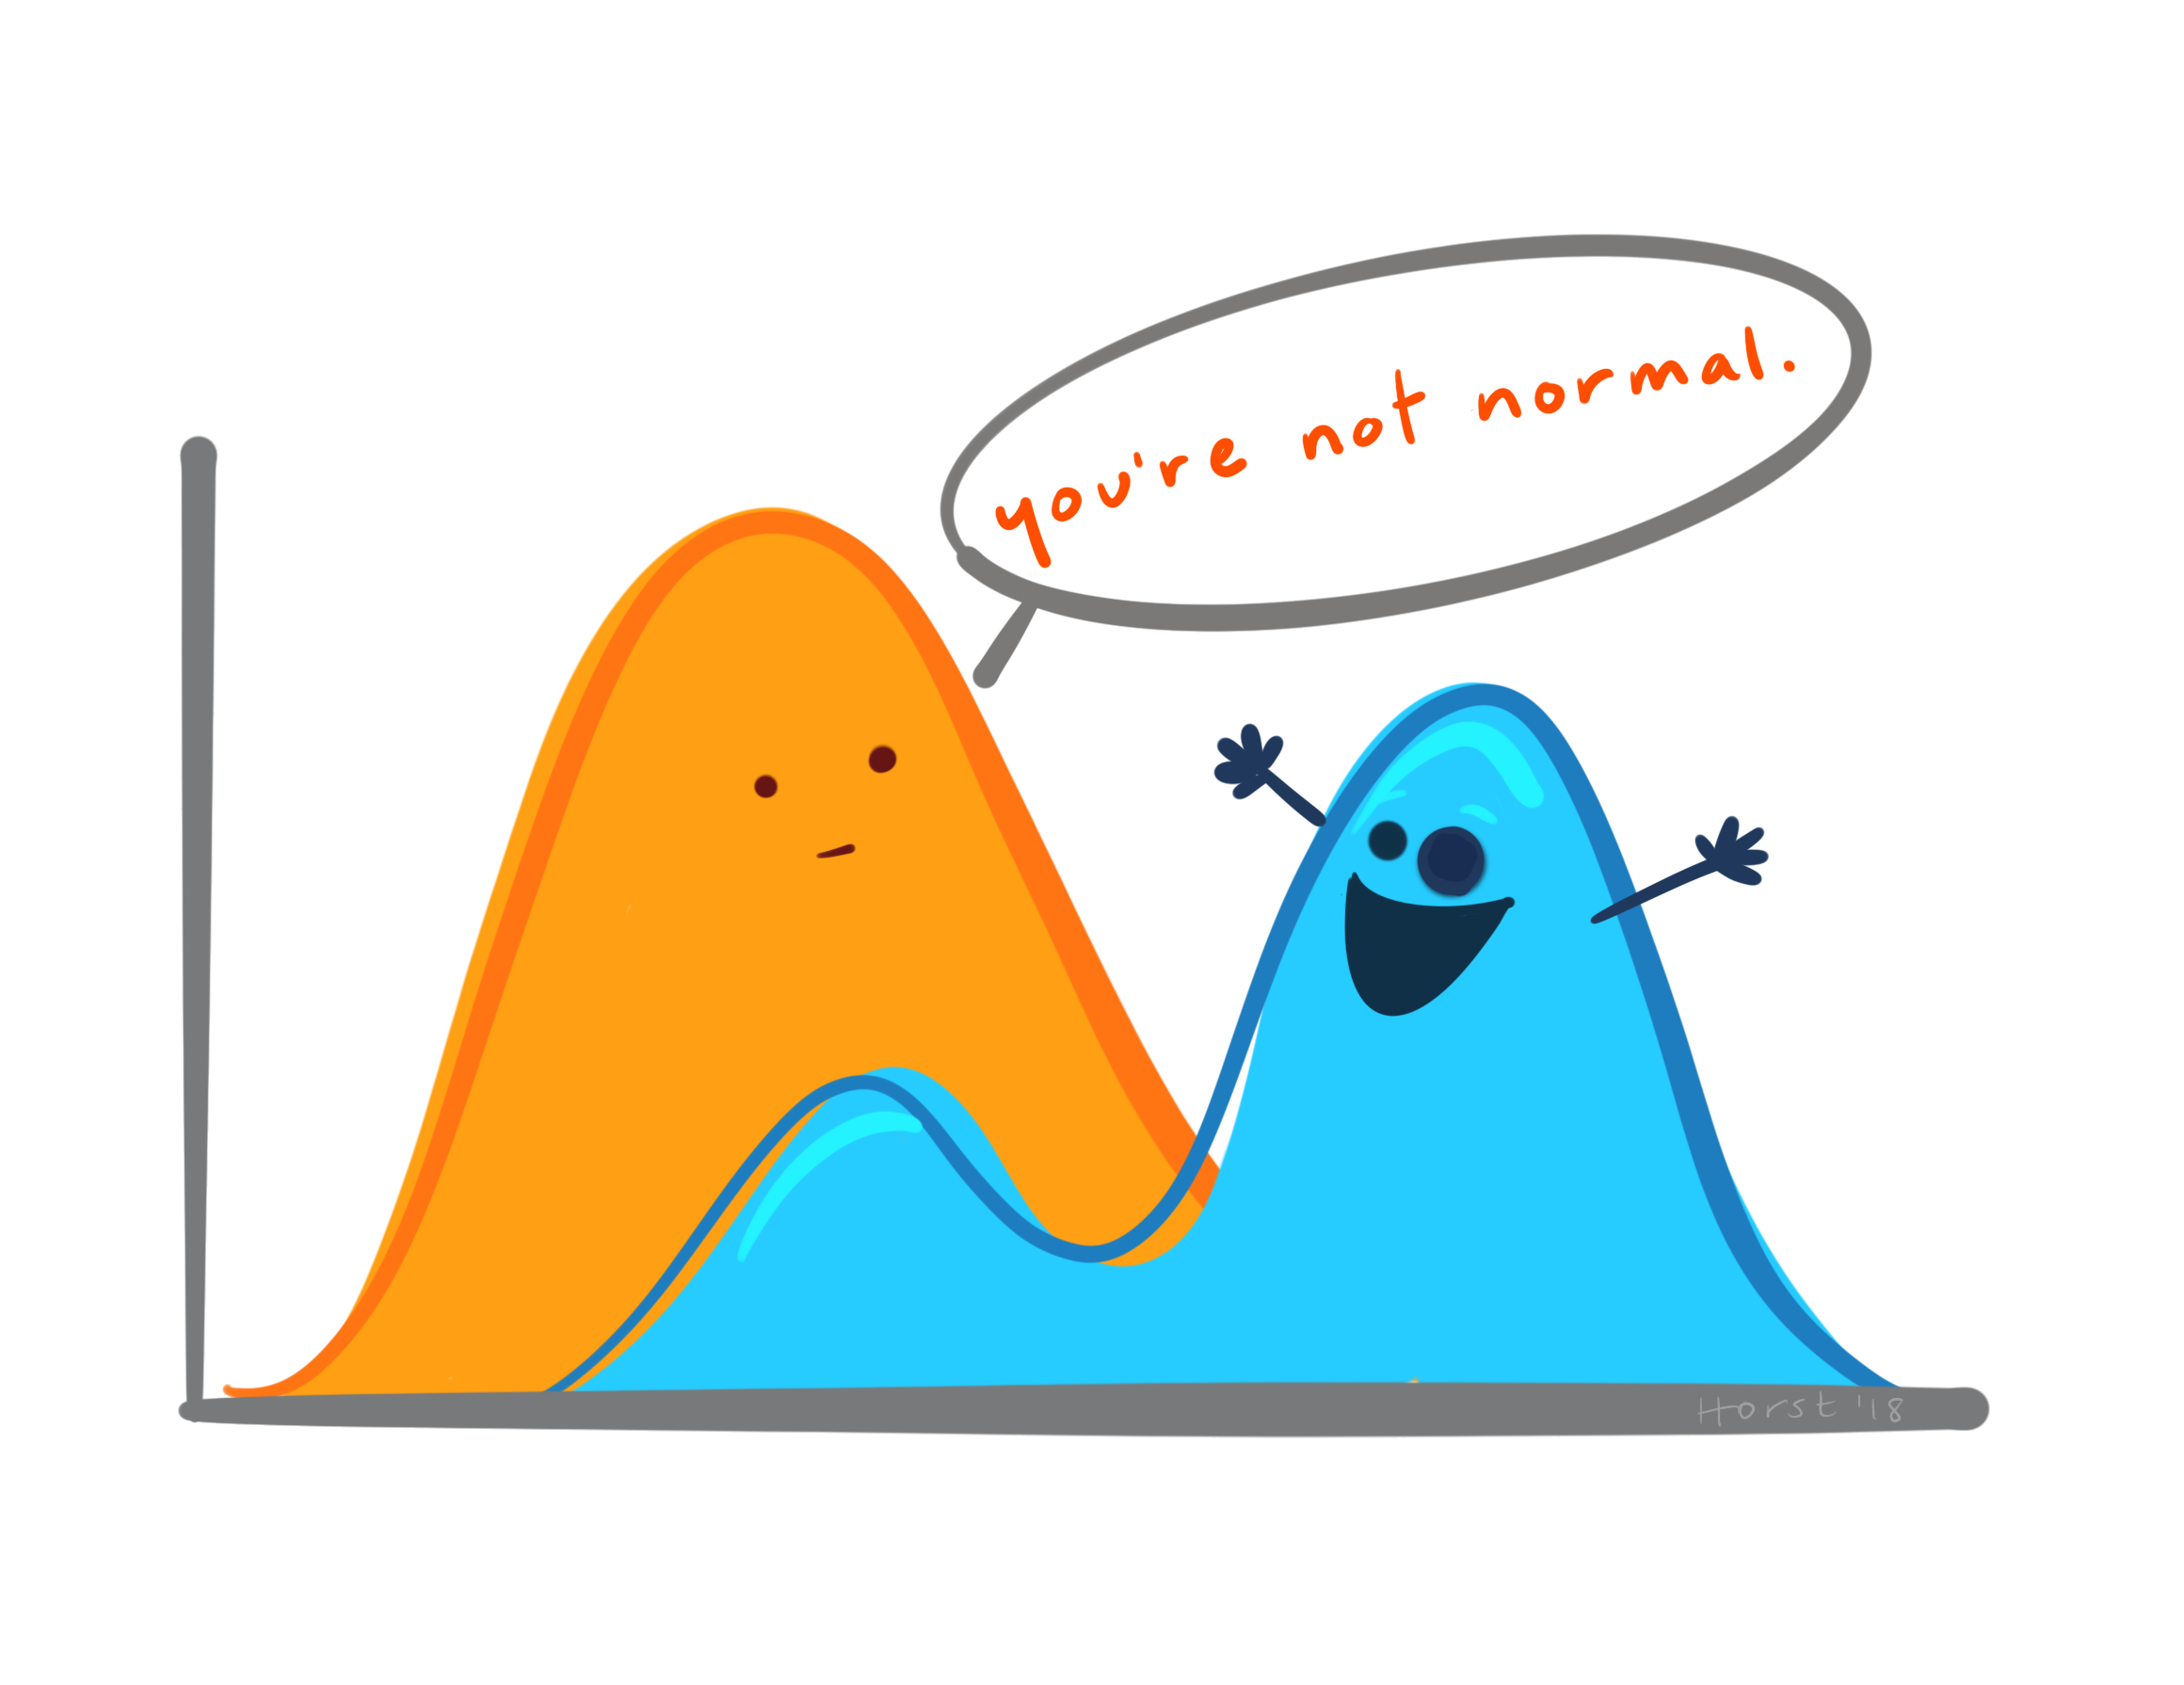
\includegraphics[width=0.9\columnwidth]{not_normal_transparent.png}
		\end{column}
	\end{columns}
\end{frame}

\subsection{Outliers}
\begin{frame}{Outliers}
	Models based on the \textbf{normal distribution are notoriously ``non-robust''
		against outliers},
	in the sense that a \textbf{single observation can greatly affect the
		inference of all model's parameters},
	even those that has a shallow relationship with it.
\end{frame}

\subsection{Overdispersion}
\begin{frame}{Overdispersion}
	\begin{defn}[Overdispersion and underdispersion]
		Superdispersion and underdispersion\footnote{
			rarer to find in the real world.}
		refer to data that have more or fewer variation than expected
		under a probability model.
		\parencite{gelman2020regression}
	\end{defn}
	\vfill
	For each one of the models we covered, there is a \textbf{natural extension}
	in which \textbf{a single parameter} is added to allow for overdispersion.
	\parencite{gelman2013bayesian}.
\end{frame}

\begin{frame}{Overdispersion Example}
	\begin{example}[Car accidents]
		Suppose you are analyzing data from car accidents.
		The model we generally use in this type of phenomena is
		\textbf{Poisson regression}.
		\vfill
		Poisson distribution has the same parameter for both the mean and variance:
		the rate parameter $\lambda$.
		\vfill
		Hence, if you find a higher variability than expected under the
		Poisson likelihood function allows,
		then probably you won't be able to model properly the desired phenomena.
	\end{example}
\end{frame}

\subsection{Overdispersion Versions of Probabilistic Models}
\subsubsection{Student's $t$ instead of Normal}
\begin{frame}{Student's $t$ instead of Normal}
	Student's $t$ distribution has \textbf{wider\footnote{or ``fatter''.} tails}
	than the Normal distribution.
	\vfill
	This makes it a good candidate to \textbf{fit outliers without
		instabilities in the parameters' inference}.
	\vfill
	From the Bayesian viewpoint, there is nothing special or magical in the
	Gaussian/Normal likelihood.
	It is just another distribution specified in a statistical model.
	We can make our model robust by using the Student's $t$ distribution
	as a likelihood function.
\end{frame}

\begin{frame}{Student's $t$ instead of Normal}
	\centering
	\begin{tikzpicture}
		\begin{axis}[every axis plot, line width=2pt,
				ylabel=PDF,
				domain=-4:4,samples=200,
				axis x line*=bottom, % no box around the plot, only x and y axis
				axis y line*=left % the * suppresses the arrow tips
			]

			\addplot [blue] {gaussian(0, 1)};
			\addlegendentry{Normal}
			\addplot [red] {student(3)};
			\addlegendentry{Student's $t$ with $\nu=3$}
		\end{axis}
	\end{tikzpicture}
\end{frame}

\begin{frame}{Student's $t$ instead of Normal}
	By using a Student's $t$ distribution instead of the Normal distribution
	as likelihood functions,
	the model's error $\sigma$ does \textit{not} follow a Normal distribution,
	but a Student's $t$ distribution:
	$$
		\begin{aligned}
			\mathbf{y}     & \sim \text{Student}\left( \nu, \alpha + \mathbf{X} \boldsymbol{\beta}, \sigma \right) \\
			\alpha             & \sim \text{Normal}(\mu_\alpha, \sigma_\alpha)                                         \\
			\boldsymbol{\beta} & \sim \text{Normal}(\mu_{\boldsymbol{\beta}}, \sigma_{\boldsymbol{\beta}})             \\
			\nu                & \sim \text{Log-Normal}(2, 1)                                                          \\
			\sigma             & \sim \text{Exponential}(\lambda_\sigma)
		\end{aligned}
	$$
	\small
	Note that we are including an extra parameter $\nu$,
	which represents the Student's $t$ distribution degrees of freedom,
	to be estimated by the model \parencite{gelman2013bayesian}.
	This controls how wide or narrow the ``tails'' of the distribution will be.
	A heavy-tailed, positive-only prior is advised.
\end{frame}

\subsubsection{Beta-Binomial instead of Binomial}
\begin{frame}{Beta-Binomial instead of the Binomial}
	The binomial distribution has a practical limitation that we only have
	one free parameter to estimate\footnote{since $n$ already comes from data.} ($p$).
	This implies in the \textbf{variance to determined by the mean}.
	Hence, the binomial distribution \textbf{cannot} tolerate overdispersion.
	\vfill
	A robust alternative is the \textbf{beta-binomial distribution}, which,
	as the name suggests, is a \textbf{beta mixture of binomials distributions}.
	Most important, it \textbf{allows that the variance to be independent of the mean},
	making it \textbf{robust against overdispersion}.
\end{frame}

\begin{frame}{Beta-Binomial instead of Binomial}
	The \textbf{beta-binomial distribution} is a binomial distribution, where
	the probability of success $p$ is parameterized as a $\text{Beta}(\alpha, \beta)$.
	\vfill
	Generally, we use $\alpha$ as the binomial's probability of the success $p$,
	and $\beta$\footnote(sometimes specified as $\phi$) is the additional parameter
	to control and allow for overdispersion.
	\vfill
	Values of $\beta \geq 1$ make the beta-binomial behave the same as a binomial.
\end{frame}

\begin{frame}{Beta-Binomial instead of Binomial}
	$$
		\begin{aligned}
			\mathbf{y}     & \sim \text{Beta-Binomial}(n, p, \phi)                                     \\
			p                  & \sim \text{Logistic/Probit}(\alpha +  \mathbf{X} \boldsymbol{\beta})     \\
			\alpha             & \sim \text{Normal}(\mu_\alpha, \sigma_\alpha)                             \\
			\boldsymbol{\beta} & \sim \text{Normal}(\mu_{\boldsymbol{\beta}}, \sigma_{\boldsymbol{\beta}}) \\
			\phi               & \sim \text{Exponential}(1)
		\end{aligned}
	$$
	\vfill
	It is also proper to include the overdispersion $\beta$ parameter as an
	additional parameter to be estimated by the model
	\parencite{gelman2013bayesian,mcelreath2020statistical}.
	A heavy-tailed, positive-only prior is advised.
\end{frame}

\subsubsection{Student's $t$ instead Binomial}
\begin{frame}{Student's $t$ instead Binomial}
	\small
	Also known as Robit\footnote{there is a great discussion between
		Gelman, Vehtari and Kurz at
		\href{https://discourse.mc-stan.org/t/robit-regression-not-robust/21245/}{
			\texttt{Stan}'s Discourse}.} \parencite{gelman2013bayesian, gelman2020regression}.
	The ideia is to make the logistic regression robust by using a
	\textbf{latent variable $z$} as the linear predictor.
	$z$'s errors, $\epsilon$, are distributed as a Student's $t$ distribution:
	$$
		\begin{aligned}
			y_i        & = \begin{cases} 0 & \text{se } z_i < 0 \\ 1 & \text{se }\ z_i > 0 \end{cases} \\
			z_i        & = X_i \boldsymbol{\beta} + \epsilon_i                                         \\
			\epsilon_i & \sim \text{Student} \left (\nu, 0, \sqrt{\frac{\nu - 2}{\nu}} \right)         \\
			\nu        & \sim \text{Gamma}(2, 0.1) \in \left[2, \infty \right)
		\end{aligned}
	$$
	\footnotesize
	Here we are using the gamma distribution as a truncated Student's $t$
	distribution for the degrees of freedom parameter $\nu \geq 2$.
	Another option would be to fix $\nu = 4$.
\end{frame}

\subsubsection{Negative Binomial instead of Poisson}
\begin{frame}{Negative Binomial instead of Poisson}
	This is the overdispersion example.
	The Poisson distribution uses a \textbf{single parameter for both its mean and variance}.
	\vfill
	Hence, if you find overdispersion, probably you'll need a robust alternative to Poisson.
	This is where the \textbf{negative binomial}, with an extra parameter $\phi$,
	that makes it \textbf{robust to overdispersion}.
	\vfill
	$\phi$ controls the probability of success $p$,
	and we generally use a gamma distribution as its prior.
	$\phi$ is also known as a ``reciprocal dispersion'' parameter.
\end{frame}

\begin{frame}{Negative Binomial instead of Poisson}
	$$
		\begin{aligned}
			\mathbf{y}     & \sim \text{Negative Binomial} \left( e^{(\alpha + \mathbf{X} \boldsymbol{\beta})}, \phi \right) \\
			\phi               & \sim \text{Gamma}(0.01, 0.01)                                                                   \\
			\alpha             & \sim \text{Normal}(\mu_\alpha, \sigma_\alpha)                                                   \\
			\boldsymbol{\beta} & \sim \text{Normal}(\mu_{\boldsymbol{\beta}}, \sigma_{\boldsymbol{\beta}})
		\end{aligned}
	$$
	\vfill
	Here we also give a heavy-tailed, positive-only prior to $\phi$.
	Something like the $\text{Gamma}(0.01, 0.01)$ works.
\end{frame}

\subsubsection{Negative Binomial Mixture instead of Poisson}
\begin{frame}{Negative Binomial Mixture instead of Poisson}
	Even using a negative binomial likelihood,
	if you encounter acute overdispersion,
	specially when there is a lot of zeros in your data
	(zero-inflated),
	your model can still perform a bad fit to the data.
	\vfill
	Another suggestion is to use a mixture of negative binomial
	\parencite{mcelreath2020statistical}.
\end{frame}

\begin{frame}{Negative Binomial Mixture instead of Poisson}
	Here, $S_i$ is a dummy variable,
	taking value $1$ if the $i$th observation has a value $\neq 0$.
	$S_i$ can be modeled using logistic regression:
	$$
		\begin{aligned}
			\mathbf{y}
			                    & \begin{cases}
				                      = 0,                                                                                             & \text{ if } S_i = 0 \\
				                      \sim \text{Negative Binomial} \left( e^{(\alpha + \mathbf{X} \boldsymbol{\beta})}, \phi \right), & \text{ if } S_i = 1
			                      \end{cases} \\
			P(S_i = 1)          & = \text{Logistic/Logit}(\mathbf{X} \boldsymbol{\gamma})                                                               \\
			\boldsymbol{\gamma} & \sim \text{Beta}(1, 1)
		\end{aligned}
	$$
	\vfill
	$\boldsymbol{\gamma}$ is a new vector of coefficients which we give uniform priors of $\text{Beta} (1, 1)$.
\end{frame}

\subsection{Why Use Non-Robust Models?}
\begin{frame}{Why Use Non-Robust Models?}
	The \textbf{central limit theorem} tells us that the \textbf{normal distribution}
	is an appropriate model for data that arises as a
	\textbf{sum of independent components}.
	\vfill
	Even when they are naturally not implicit in a phenomena structure,
	\textbf{simpler non-robust models are computational efficient}.
	\vfill
	Of course, you must always guide the model choice in a
	\textbf{principled manner},
	taking into account the underlying phenomena data generating process.
	And make sure to make \textbf{posterior predictive checks}.
\end{frame}

% !TeX root = slides.tex
\section{Hierarchical Models}

\subsection{Hierarchical Models - Recommended References}
\begin{frame}{Hierarchical Models - Recommended References}
	\begin{vfilleditems}
		\item \textcite{gelman2013bayesian}:
		\begin{vfilleditems}
			\item Chapter 5: Hierarchical models
			\item Chapter 15: Hierarchical linear models
		\end{vfilleditems}
		\item \textcite{mcelreath2020statistical}:
		\begin{vfilleditems}
			\item Chapter 13: Models With Memory
			\item Chapter 14: Adventures in Covariance
		\end{vfilleditems}
		\item \textcite{gelmanDataAnalysisUsing2007}
		\item Michael Betancourt's case study on \href{https://betanalpha.github.io/assets/case_studies/hierarchical_modeling.html}{Hierarchical modeling}
		\item \textcite{kruschke2015bayesian}
	\end{vfilleditems}
\end{frame}

\subsection{What are hierarchical models?}
\begin{frame}{I have many names...}
	Hierarchical models are also known for several names\footnote{
		for the whole full list
		\href{https://statmodeling.stat.columbia.edu/2019/09/18/all-the-names-for-hierarchical-and-multilevel-modeling/}{check here}.}:
	\begin{vfilleditems}
		\item Hierarchical Models
		\item Random Effects Models
		\item Mixed Effects Models
		\item Cross-Sectional Models
		\item Nested Data Models
	\end{vfilleditems}
\end{frame}

\begin{frame}{What are hierarchical models?}
	\begin{defn}[Hierarchical Model]
		Statistical model specified in multiple levels that estimates
		parameters from the posterior distribution using a Bayesian approach.
		The sub-models inside the model combines to form a hierarchical model,
		and Bayes' theorem is used to integrate it to observed data and
		account for all uncertain.
	\end{defn}
	\vfill
	Hierarchical models are mathematical descriptions that involves several parameters,
	where some parameters' estimates depend on another parameters' values.
\end{frame}

\begin{frame}{What are Hierarchical Models?\footnote{figure adapted from \href{https://betanalpha.github.io/assets/case_studies/hierarchical_modeling.html}{Michael Betancourt (CC-BY-SA-4.0)}}}
	\small
	Hyperparameter $\phi$ that parameterizes $\theta_1, \theta_2, \dots, \theta_K$,
	that are used to infer the posterior density of some random variable
	$\mathbf{y} = y_1, y_2, \dots, y_K$
	\begin{adjustbox}{max width=1.0\textwidth}
		\begin{tikzpicture}[scale=0.275, thick]

			\pgfmathsetmacro{\r}{2}
			\pgfmathsetmacro{\dx}{0}
			\pgfmathsetmacro{\dy}{0}

			\draw[black] (-21 + \dx, -7 + \dy) rectangle (21 + \dx, 13 + \dy);

			\filldraw[fill=dark, draw=dark, line width=1.5] (-12 + \dx, 9 + \dy) circle (\r)
			node[color=white] { $y_{1}$ };

			\filldraw[fill=dark, draw=dark, line width=1.5] (-6 + \dx, 9 + \dy) circle (\r)
			node[color=white] { $\ldots$ };

			\filldraw[fill=dark, draw=dark, line width=1.5] (0 + \dx, 9 + \dy) circle (\r)
			node[color=white] { $y_{k}$ };

			\filldraw[fill=dark, draw=dark, line width=1.5] (6 + \dx, 9 + \dy) circle (\r)
			node[color=white] { $\ldots$ };

			\filldraw[fill=dark, draw=dark, line width=1.5] (12 + \dx, 9 + \dy) circle (\r)
			node[color=white] { $y_{K}$ };

			\draw[->, >=stealth, color=mid, line width=1.5] (-12 + \dx, 3 + \r + \dy) -- (-12 + \dx, 9 - \r + \dy);
			\draw[->, >=stealth, color=mid, line width=1.5] (-6 + \dx, 3 + \r + \dy) -- (-6 + \dx, 9 - \r + \dy);
			\draw[->, >=stealth, color=mid, line width=1.5] (0 + \dx, 3 + \r + \dy) -- (0 + \dx, 9 - \r + \dy);
			\draw[->, >=stealth, color=mid, line width=1.5] (6 + \dx, 3 + \r + \dy) -- (6 + \dx, 9 - \r + \dy);
			\draw[->, >=stealth, color=mid, line width=1.5] (12 + \dx, 3 + \r + \dy) -- (12 + \dx, 9 - \r + \dy);

			\filldraw[fill=black, draw=dark, line width=1.5] (-12 + \dx, 3 + \dy) circle (\r)
			node[color=white] { $\theta_{1}$ };

			\filldraw[fill=black, draw=dark, line width=1.5] (-6 + \dx, 3 + \dy) circle (\r)
			node[color=white] { $\ldots$ };

			\filldraw[fill=black, draw=dark, line width=1.5] (0 + \dx, 3 + \dy) circle (\r)
			node[color=white] { $\theta_{k}$ };

			\filldraw[fill=black, draw=dark, line width=1.5] (6 + \dx, 3 + \dy) circle (\r)
			node[color=white] { $\ldots$ };

			\filldraw[fill=black, draw=dark, line width=1.5] (12 + \dx, 3 + \dy) circle (\r)
			node[color=white] { $\theta_{K}$ };

			\draw[->, >=stealth, color=mid, line width=1.5] (0 + \dx, -3 + \r + \dy) -- (-12 + \dx, 3 - \r + \dy);
			\draw[->, >=stealth, color=mid, line width=1.5] (0 + \dx, -3 + \r + \dy) -- (-6 + \dx, 3 - \r + \dy);
			\draw[->, >=stealth, color=mid, line width=1.5] (0 + \dx, -3 + \r + \dy) -- (0 + \dx, 3 - \r + \dy);
			\draw[->, >=stealth, color=mid, line width=1.5] (0 + \dx, -3 + \r + \dy) -- (6 + \dx, 3 - \r + \dy);
			\draw[->, >=stealth, color=mid, line width=1.5] (0 + \dx, -3 + \r + \dy) -- (12 + \dx, 3 - \r + \dy);

			\filldraw[fill=black, draw=dark, line width=1.5] (0 + \dx, -3 + \dy) circle (\r)
			node[color=white] { $\phi$ };

		\end{tikzpicture}
	\end{adjustbox}
\end{frame}

\begin{frame}{What are Hierarchical Models?\footnote{figure adapted from \href{https://betanalpha.github.io/assets/case_studies/hierarchical_modeling.html}{Michael Betancourt (CC-BY-SA-4.0)}}}
	\footnotesize
	Even that the observations directly inform only a single set of parameters,
	a hierarchical model couples individual parameters,
	and provides a ``backdoor'' for information flow.
	\begin{adjustbox}{max width=1.0\textwidth}
		\begin{tikzpicture}[scale=0.3, thick]

			% Right
			\pgfmathsetmacro{\r}{2}

			\pgfmathsetmacro{\dx}{0}
			\pgfmathsetmacro{\dy}{0}

			\draw[black] (-17 + \dx, -7 + \dy) rectangle (17 + \dx, 13 + \dy);

			\fill[fill=dark, line width=1.5, opacity=0.50] (-12 + \dx, 9 + \dy) circle (\r)
			node[color=white] { $y_{1}$ };

			\fill[fill=dark, line width=1.5, opacity=0.50] (-6 + \dx, 9 + \dy) circle (\r)
			node[color=white] { $\ldots$ };

			\filldraw[fill=dark, draw=dark, line width=1.5] (0 + \dx, 9 + \dy) circle (\r)
			node[color=white] { $y_{k}$ };

			\fill[fill=dark, line width=1.5, opacity=0.50] (6 + \dx, 9 + \dy) circle (\r)
			node[color=white] { $\ldots$ };

			\fill[fill=dark, line width=1.5, opacity=0.50] (12 + \dx, 9 + \dy) circle (\r)
			node[color=white] { $y_{K}$ };

			\draw[<-, >=stealth, color=dark, line width=1.5] (0 + \dx, 3 + \r + \dy) -- (0 + \dx, 9 - \r + \dy);

			\filldraw[fill=black, draw=dark, line width=1.5] (-12 + \dx, 3 + \dy) circle (\r)
			node[color=white] { $\theta_{1}$ };

			\filldraw[fill=black, draw=dark, line width=1.5,] (-6 + \dx, 3 + \dy) circle (\r)
			node[color=white] { $\ldots$ };

			\filldraw[fill=black, draw=dark, line width=1.5] (0 + \dx, 3 + \dy) circle (\r)
			node[color=white] { $\theta_{k}$ };

			\filldraw[fill=black, draw=dark, line width=1.5] (6 + \dx, 3 + \dy) circle (\r)
			node[color=white] { $\ldots$ };

			\filldraw[fill=black, draw=dark, line width=1.5] (12 + \dx, 3 + \dy) circle (\r)
			node[color=white] { $\theta_{K}$ };

			\draw[->, >=stealth, color=dark, line width=1.5] (0 + \dx, -3 + \r + \dy) -- (-12 + \dx, 3 - \r + \dy);
			\draw[->, >=stealth, color=dark, line width=1.5] (0 + \dx, -3 + \r + \dy) -- (-6 + \dx, 3 - \r + \dy);
			\draw[<-, >=stealth, color=dark, line width=1.5] (0 + \dx, -3 + \r + \dy) -- (0 + \dx, 3 - \r + \dy);
			\draw[->, >=stealth, color=dark, line width=1.5] (0 + \dx, -3 + \r + \dy) -- (6 + \dx, 3 - \r + \dy);
			\draw[->, >=stealth, color=dark, line width=1.5] (0 + \dx, -3 + \r + \dy) -- (12 + \dx, 3 - \r + \dy);

			\filldraw[fill=black, draw=dark, line width=1.5] (0 + \dx, -3 + \dy) circle (\r)
			node[color=white] { $\phi$ };

			% Left
			\pgfmathsetmacro{\dx}{35}
			\pgfmathsetmacro{\dy}{0}

			\draw[black] (-17 + \dx, -7 + \dy) rectangle (17 + \dx, 13 + \dy);

			\filldraw[fill=dark,  draw=dark, line width=1.5] (-12 + \dx, 9 + \dy) circle (\r)
			node[color=white] { $y_{1}$ };

			\filldraw[fill=dark,  draw=dark, line width=1.5] (-6 + \dx, 9 + \dy) circle (\r)
			node[color=white] { $\ldots$ };

			\fill[fill=dark, line width=1.5, opacity=0.50] (0 + \dx, 9 + \dy) circle (\r)
			node[color=white] { $y_{k}$ };

			\filldraw[fill=dark, draw=dark, line width=1.5] (6 + \dx, 9 + \dy) circle (\r)
			node[color=white] { $\ldots$ };

			\filldraw[fill=dark, draw=dark, line width=1.5] (12 + \dx, 9 + \dy) circle (\r)
			node[color=white] { $y_{K}$ };

			\draw[<-, >=stealth, color=dark, line width=1.5] (-12 + \dx, 3 + \r + \dy) -- (-12 + \dx, 9 - \r + \dy);
			\draw[<-, >=stealth, color=dark, line width=1.5] (-6 + \dx, 3 + \r + \dy) -- (-6 + \dx, 9 - \r + \dy);
			\draw[<-, >=stealth, color=dark, line width=1.5] (6 + \dx, 3 + \r + \dy) -- (6 + \dx, 9 - \r + \dy);
			\draw[<-, >=stealth, color=dark, line width=1.5] (12 + \dx, 3 + \r + \dy) -- (12 + \dx, 9 - \r + \dy);

			\filldraw[fill=black, draw=dark, line width=1.5] (-12 + \dx, 3 + \dy) circle (\r)
			node[color=white] { $\theta_{1}$ };

			\filldraw[fill=black, draw=dark, line width=1.5,] (-6 + \dx, 3 + \dy) circle (\r)
			node[color=white] { $\ldots$ };

			\filldraw[fill=black, draw=dark, line width=1.5] (0 + \dx, 3 + \dy) circle (\r)
			node[color=white] { $\theta_{k}$ };

			\filldraw[fill=black, draw=dark, line width=1.5] (6 + \dx, 3 + \dy) circle (\r)
			node[color=white] { $\ldots$ };

			\filldraw[fill=black, draw=dark, line width=1.5] (12 + \dx, 3 + \dy) circle (\r)
			node[color=white] { $\theta_{K}$ };

			\draw[<-, >=stealth, color=dark, line width=1.5] (-\r + \dx, -3 + \dy) -- (-12 + \dx, 3 - \r + \dy);
			\draw[<-, >=stealth, color=dark, line width=1.5] ({-0.25 - \r * cos(45) + \dx}, {-3 + \r * cos(45) + \dy}) -- (-6 + \dx, 3 - \r + \dy);
			\draw[->, >=stealth, color=dark, line width=1.5] (0 + \dx, -3 + \r + \dy) -- (0 + \dx, 3 - \r + \dy);
			\draw[<-, >=stealth, color=dark, line width=1.5] ({0.25 + \r * cos(45) + \dx}, {-3 + \r * cos(45) + \dy}) -- (6 + \dx, 3 - \r + \dy);
			\draw[<-, >=stealth, color=dark, line width=1.5] (\r + \dx, -3 + \dy) -- (12 + \dx, 3 - \r + \dy);

			\filldraw[fill=black, draw=dark, line width=1.5] (0 + \dx, -3 + \dy) circle (\r)
			node[color=white] { $\phi$ };
		\end{tikzpicture}
	\end{adjustbox}

	\footnotesize
	For example, the observations from the $k$th group, $y_k$,
	informs directly the parameters that quantify the $k$th group's behavior,
	$\theta_k$.
	These parameters, however, inform directly the population-level parameters,
	$\phi$, that, in turn, informs others group-level parameters.
	In the same manner, observations that informs directly other group's parameters
	also provide indirectly information to population-level parameters,
	which then informs other group-level parameters, and so on...
\end{frame}

\subsection{When to Use Hierarchical Models?}
\begin{frame}{When to Use Hierarchical Models?}
	\textbf{Hierarchical models} are used when information is available in
	\textbf{several levels of units of observation}.
	The hierarchical structure of analysis and organization assists in the
	understanding of \textbf{multiparameter problems},
	while also performing a crucial role in the development of
	\textbf{computational strategies}.
\end{frame}

\begin{frame}{When to Use Hierarchical Models?}
	Hierarchical models are particularly appropriate for research projects
	where participant data can be organized in more than one level\footnote{
		also known as nested data.}.
	The units of analysis are generally individuals that are nested inside
	contextual/aggregate units (groups).
	\vfill
	\small
	An example is when we measure individual performance
	and we have additional information about distinct group membership such as:
	\begin{vfilleditems}
		\item \small sex
		\item \small age group
		\item \small income level
		\item \small education level
		\item \small state/province of residence
	\end{vfilleditems}
\end{frame}

\begin{frame}{When to Use Hierarchical Models?}
	Another good use case is \textbf{big data} \parencite{gelman2013bayesian}.
	\begin{vfilleditems}
		\item simple nonhierarchical models are usually inappropriate for hierarchical data:
		with few parameters,
		they generally \textit{cannot} fit large datasets accurately.
		\item whereas with many parameters, they tend to \textbf{overfit}.
		\item hierarchical models can have enough parameters to fit the data well,
		while using a population distribution to structure some dependence into the parameters,
		thereby \textbf{avoiding problems of overfitting}.
	\end{vfilleditems}
\end{frame}

\begin{frame}{When to Use Hierarchical Models?}
	Most important is \textbf{not to violate} the \textbf{exchangeability assumption}
	\parencite{definettiTheoryProbability1974}.
	\vfill
	This assumption stems from the principle that \textbf{groups are \textit{exchangeable}}.
\end{frame}

\begin{frame}{Exchangeability \parencite{definettiTheoryProbability1974}\footnote{figures adapted from \href{https://betanalpha.github.io/assets/case_studies/hierarchical_modeling.html}{Michael Betancourt (CC-BY-SA-4.0)}.}}
	\begin{adjustbox}{max width=1.0\textwidth}
		\begin{tikzpicture}[scale=0.3, thick]

			% Left
			\begin{scope}[shift={(-36, 0)}]

				\draw[white] (-17, 0) rectangle (17, 15);

				\fill[dark] (-10, 4) circle (1);
				\begin{scope}
					\clip (-10, 4) circle (1);
					\draw[color=light, line width=5, rotate=30] (-5.25, 8.25) arc[x radius=1.4, y radius=0.2, start angle=0, end angle=-180];
				\end{scope}
				\node at (-10, 10) {
\includegraphics[width=2cm]{cup_up.png}};

				\fill[mid] (0, 4) circle (1);
				\begin{scope}
					\clip (0, 4) circle (1);
					\draw[color=dark, line width=2] (1.1, 4.3) arc[x radius=1.1, y radius=0.2, start angle=0, end angle=180];
					\draw[color=dark, line width=2] (1.1, 3.7) arc[x radius=1.1, y radius=0.2, start angle=0, end angle=180];
				\end{scope}
				\node at (0, 10) {
\includegraphics[width=2cm]{cup_up.png}};

				\fill[dark] (+10, 4) circle (1);
				\begin{scope}
					\clip (10, 4) circle (1);
					\draw[color=mid, line width=1] (10, 3) -- (10, 5);
					\draw[color=mid, line width=1] (10.25, 5) arc[x radius=0.3, y radius=1.1, start angle=90, end angle=-90];
					\draw[color=mid, line width=1] (9.75, 5) arc[x radius=0.3, y radius=1.1, start angle=90, end angle=270];
				\end{scope}
				\node at (+10, 10) {
\includegraphics[width=2cm]{cup_up.png}};

			\end{scope}

			% Right
			\begin{scope}[shift={(0, 0)}]

				\draw[white] (-17, 0) rectangle (17, 15);

				\fill[dark] (-10, 4) circle (1);
				\node at (-10, 7) {
\includegraphics[width=2cm]{cup_down.png}};
				\begin{scope}[scale=0.7, shift={(-17, 3)}, rotate=-5]
					\fill[dark, rounded corners=3] (0, 0) rectangle (10, 6);
					\fill[black] (0, 0.5) rectangle (10, 3.5);
					\node[text=white, align=center, rotate=-5] at (5, 5.2) { \small \textsf{HELLO} };
					\node[text=white, align=center, rotate=-5] at (5, 4.1) { \tiny \textsf{my name is} };
					\node[text=white, align=center, rotate=0] at (5.25, 2) { \large \textsl{Group 1} };
				\end{scope}

				\fill[dark] (0, 4) circle (1);
				\node at (0, 7) {
\includegraphics[width=2cm]{cup_down.png}};
				\begin{scope}[scale=0.7, shift={(-2, 3)}, rotate=10]
					\fill[dark, rounded corners=3] (0, 0) rectangle (10, 6);
					\fill[black] (0, 0.5) rectangle (10, 3.5);
					\node[text=white, align=center, rotate=10] at (5, 5.2) { \small \textsf{HELLO} };
					\node[text=white, align=center, rotate=10] at (5, 4.1) { \tiny \textsf{my name is } };
					\node[text=white, align=center, rotate=7] at (5.25, 2) { \large \textsl{Group 2} };
				\end{scope}

				\fill[dark] (+10, 4) circle (1);
				\node at (+10, 7) {
\includegraphics[width=2cm]{cup_down.png}};
				\begin{scope}[scale=0.7, shift={(12, 3)}, rotate=1]
					\fill[dark, rounded corners=3] (0, 0) rectangle (10, 6);
					\fill[black] (0, 0.5) rectangle (10, 3.5);
					\node[text=white, align=center, rotate=1] at (5, 5.2) { \small \textsf{HELLO} };
					\node[text=white, align=center, rotate=1] at (5, 4.1) { \tiny \textsf{my name is } };
					\node[text=white, align=center, rotate=1] at (5.25, 2) { \large \textsl{Group 3} };
				\end{scope}
			\end{scope}
		\end{tikzpicture}
	\end{adjustbox}
\end{frame}

\begin{frame}{Exchangeability \parencite{definettiTheoryProbability1974}\footnote{figures adapted from \href{https://betanalpha.github.io/assets/case_studies/hierarchical_modeling.html}{Michael Betancourt (CC-BY-SA-4.0)}.}}
	\begin{adjustbox}{max width=1.0\textwidth}
		\begin{tikzpicture}[scale=0.3, thick]


			\draw[white] (-17, -3) rectangle (17, 15);

			\fill[dark] (-10, 4) circle (1);
			\node at (-10, 7) {
\includegraphics[width=2cm]{cup_down.png}};

			% Left
			\begin{scope}[scale=0.7, shift={(-17, 3)}, rotate=-5]
				\fill[dark, rounded corners=3] (0, 0) rectangle (10, 6);
				\fill[black] (0, 0.5) rectangle (10, 3.5);
				\node[text=white, align=center, rotate=-5] at (5, 5.2) { \small \textsf{HELLO} };
				\node[text=white, align=center, rotate=-5] at (5, 4.1) { \tiny \textsf{my name is } };
				\node[text=white, align=center, rotate=0] at (5.25, 2) { \large \textsl{Group 1} };
			\end{scope}

			\fill[dark] (0, 4) circle (1);
			\node at (0, 7) {
\includegraphics[width=2cm]{cup_down.png}};

			\begin{scope}[scale=0.7, shift={(-2, 3)}, rotate=10]
				\fill[dark, rounded corners=3] (0, 0) rectangle (10, 6);
				\fill[black] (0, 0.5) rectangle (10, 3.5);
				\node[text=white, align=center, rotate=10] at (5, 5.2) { \small \textsf{HELLO} };
				\node[text=white, align=center, rotate=10] at (5, 4.1) { \tiny \textsf{my name is } };
				\node[text=white, align=center, rotate=7] at (5.25, 2) { \large \textsl{Group 2} };
			\end{scope}

			\fill[dark] (+10, 4) circle (1);
			\node at (+10, 7) {
\includegraphics[width=2cm]{cup_down.png}};

			\begin{scope}[scale=0.7, shift={(12, 3)}, rotate=1]
				\fill[dark, rounded corners=3] (0, 0) rectangle (10, 6);
				\fill[black] (0, 0.5) rectangle (10, 3.5);
				\node[text=white, align=center, rotate=1] at (5, 5.2) { \small \textsf{HELLO} };
				\node[text=white, align=center, rotate=1] at (5, 4.1) { \tiny \textsf{my name is } };
				\node[text=white, align=center, rotate=1] at (5.25, 2) { \large \textsl{Group 3} };
			\end{scope}

			\pgfmathsetmacro{\r}{10}
			\pgfmathsetmacro{\start}{160}
			\pgfmathsetmacro{\stop}{20}

			\draw[dark, <->, >=stealth] ({0 + \r * cos(\start)}, {8 + \r * sin(\start)})
			arc[x radius = \r, y radius = 3, start angle=\start, end angle= \stop];

			\pgfmathsetmacro{\r}{3}
			\pgfmathsetmacro{\start}{160}
			\pgfmathsetmacro{\stop}{20}

			\draw[dark, <->, >=stealth] ({-5 + \r * cos(\start)}, {10 + \r * sin(\start)})
			arc[x radius = \r, y radius = 0.75, start angle=\start, end angle= \stop];

			\draw[dark, <->, >=stealth] ({5 + \r * cos(\start)}, {10 + \r * sin(\start)})
			arc[x radius = \r, y radius = 0.75, start angle=\start, end angle= \stop];

			% Right
			\begin{scope}[shift={(36, 0)}]

				\draw[white] (-17, -3) rectangle (17, 15);

				\fill[dark] (-10, 4) circle (1);
				\node at (-10, 7) {
\includegraphics[width=2cm]{cup_down.png}};

				\begin{scope}[scale=0.7, shift={(-17, 3)}, rotate=-5]
					\fill[dark, rounded corners=3] (0, 0) rectangle (10, 6);
					\fill[black] (0, 0.5) rectangle (10, 3.5);
					\node[text=white, align=center, rotate=-5] at (5, 5.2) { \small \textsf{HELLO} };
					\node[text=white, align=center, rotate=-5] at (5, 4.1) { \tiny \textsf{my name is } };
					\node[text=white, align=center, rotate=0] at (5.25, 2) { \large \textsl{Group 3} };
				\end{scope}

				\fill[dark] (0, 4) circle (1);
				\node at (0, 7) {
\includegraphics[width=2cm]{cup_down.png}};

				\begin{scope}[scale=0.7, shift={(-2, 3)}, rotate=10]
					\fill[dark, rounded corners=3] (0, 0) rectangle (10, 6);
					\fill[black] (0, 0.5) rectangle (10, 3.5);
					\node[text=white, align=center, rotate=10] at (5, 5.2) { \small \textsf{HELLO} };
					\node[text=white, align=center, rotate=10] at (5, 4.1) { \tiny \textsf{my name is } };
					\node[text=white, align=center, rotate=7] at (5.25, 2) { \large \textsl{Group 1} };
				\end{scope}

				\fill[dark] (+10, 4) circle (1);
				\node at (+10, 7) {
\includegraphics[width=2cm]{cup_down.png}};

				\begin{scope}[scale=0.7, shift={(12, 3)}, rotate=1]
					\fill[dark, rounded corners=3] (0, 0) rectangle (10, 6);
					\fill[black] (0, 0.5) rectangle (10, 3.5);
					\node[text=white, align=center, rotate=1] at (5, 5.2) { \small \textsf{HELLO} };
					\node[text=white, align=center, rotate=1] at (5, 4.1) { \tiny \textsf{my name is } };
					\node[text=white, align=center, rotate=1] at (5.25, 2) { \large \textsl{Group 2} };
				\end{scope}

				\draw[light, <->, >=stealth, line width=4]
				(-8, 6.5) .. controls (-7, 7.5) and (-6.5, 8.25) ..
				(-4.5, 8.5) .. controls (-2.5, 8.75) and (-1, 8.5) .. (0, 7);
				\draw[dark, <->, >=stealth, line width=2]
				(-7.85, 6.65) .. controls (-7, 7.5) and (-6.5, 8.25) ..
				(-4.5, 8.5) .. controls (-2.5, 8.75) and (-1, 8.5) .. (-0.15, 7.15);

				\draw[light, <->, >=stealth, line width=4]
				(3, 7.5) .. controls (4, 9) and (6.25, 9.75) ..
				(8.25, 9.5) .. controls (10.25, 9.25) and (11, 8.75) .. (12, 6.75);
				\draw[dark, <->, >=stealth, line width=2]
				(3.15, 7.65) .. controls (4, 9) and (6.25, 9.75) ..
				(8.25, 9.5) .. controls (10.25, 9.25) and (11, 8.75) .. (11.9, 6.9);

				\draw[light, <->, >=stealth, line width=4]
				(-8, 1.5) .. controls (-7, -1.5) and (2, -1.25) ..
				(4, -1) .. controls (6, -0.75) and (11, -0.5) .. (12, 1.5);
				\draw[dark, <->, >=stealth, line width=2]
				(-7.925, 1.25) .. controls (-7, -1.5) and (2, -1.25) ..
				(4, -1) .. controls (6, -0.75) and (11, -0.5) .. (11.9, 1.3);

			\end{scope}

		\end{tikzpicture}
	\end{adjustbox}
\end{frame}

\subsection{Hyperprior}
\begin{frame}{Hyperprior}
	In hierarchical models, we have a hyperprior,
	which is a prior's prior:
	$$
		\begin{aligned}
			\mathbf{y}          & \sim \text{Normal}(10, \boldsymbol{\theta}) \\
			\boldsymbol{\theta} & \sim \text{Normal}(0, \phi)                 \\
			\phi                & \sim \text{Exponential(1)}
		\end{aligned}
	$$
	Here $\mathbf{y}$ is a variable of interest that belongs to distinct groups.
	$\boldsymbol{\theta}$, a prior for $\mathbf{y}$,
	is a vector of group-leve parameters with their own prior
	(which becomes a hiperprior) $\phi$.
\end{frame}

\subsection{Frequentist versus Bayesian Approaches}
\begin{frame}{Frequentist versus Bayesian Approaches}
	There are also hierarchical models in frequentist statistics.
	They are mainly available in the \texttt{lme4} package \parencite{lme4},
	and also in \texttt{MixedModels.jl} \parencite{MixedModels}.
	\begin{vfilleditems}
		\item \textbf{optimization of the likelihood function} versus \textbf{posterior approximation via MCMC}.
		Almost always lead to convergence failure for models that are not extremely simple.
		\item \textbf{frequentist hierarchical models do not compute $p$-values for the group-level effects}\footnote{
			see \href{https://stat.ethz.ch/pipermail/r-help/2006-May/094765.html}
			{Douglas Bates, creator of the \texttt{lme4} package explanation}.}.
		This is due to the underlying assumptions of the approximations that frequentist
		statistics has to to do in order to calculate the group-level effects $p$-values.
		The main one being that the groups must be balanced.
		In other words, the groups must be homogeneous in size.
		Hence, any unbalance in group compositions results in pathological $p$-values
		that should not be trusted.
	\end{vfilleditems}
\end{frame}

\begin{frame}{Frequentist versus Bayesian Approaches}
	To sum up, \textbf{frequentist approach for hierarchical models is not robust}
	in both the \textbf{inference process}
	(\textbf{convergence flaws} during the maximum likelihood estimation),
	and also in the \textbf{results} from the inference process
	(do not provide $p$-values due to
	\textbf{strong assumptions that are almost always violated}).
\end{frame}

\subsection{Approaches to Hierarchical Modeling}
\begin{frame}{Approaches to Hierarchical Modeling}
	\begin{vfilleditems}
		\item \textbf{Varying-intercept} model:
		One group-level intercept besides the population-level coefficients.
		\item \textbf{Varying-slope} model:
		One or more group-level coefficient(s) besides the population-level intercept.
		\item \textbf{Varying-intercept-slope} model:
		One group-level intercept and one or more group-level coefficient(s).
	\end{vfilleditems}
\end{frame}

\begin{frame}{Mathematical Specification of Hierarchical Models}
	We have $N$ observations organized in $J$ groups with $K$ independent variables.
\end{frame}

\begin{frame}{Mathematical Specification -- Varying-Intercept Model}
	This example is for linear regression:
	$$
		\begin{aligned}
			\mathbf{y}         & \sim \text{Normal}\left(\alpha_j + \mathbf{X} \cdot \boldsymbol{\beta}, \sigma \right) \\
			\alpha_j           & \sim \text{Normal}(\alpha, \tau)                                                       \\
			\alpha             & \sim \text{Normal}(\mu_\alpha, \sigma_\alpha)                                          \\
			\boldsymbol{\beta} & \sim \text{Normal}(\mu_{\boldsymbol{\beta}}, \sigma_{\boldsymbol{\beta}})              \\
			\tau               & \sim \text{Cauchy}^+(0, \psi_{\alpha})                                                 \\
			\sigma             & \sim \text{Exponential}(\lambda_\sigma)
		\end{aligned}
	$$
\end{frame}

\begin{frame}{Mathematical Specification -- Varying-Intercept Model}
	If you need to extend to more than one group,
	such as $J_1, J_2, \dots$:
	$$
		\begin{aligned}
			\mathbf{y}         & \sim \text{Normal}(\alpha_{j1} + \alpha_{j2} + \mathbf{X} \boldsymbol{\beta}, \sigma) \\
			\alpha_{j1}        & \sim \text{Normal}(\alpha_1, \tau_{\alpha j1})                                        \\
			\alpha_{j2}        & \sim \text{Normal}(\alpha_2, \tau_{\alpha j2})                                        \\
			\alpha_1           & \sim \text{Normal}(\mu_{\alpha 1}, \sigma_{\alpha 1})                                 \\
			\alpha_2           & \sim \text{Normal}(\mu_{\alpha 2}, \sigma_{\alpha 2})                                 \\
			\boldsymbol{\beta} & \sim \text{Normal}(\mu_{\boldsymbol{\beta}}, \sigma_{\boldsymbol{\beta}})             \\
			\tau_{\alpha j1}   & \sim \text{Cauchy}^+(0, \psi_{\alpha j1})                                             \\
			\tau_{\alpha j2}   & \sim \text{Cauchy}^+(0, \psi_{\alpha j2})                                             \\
			\sigma             & \sim \text{Exponential}(\lambda_\sigma)
		\end{aligned}
	$$
\end{frame}

\begin{frame}{Mathematical Specification -- Varying-(Intercept-)Slope Model}
	If we want a varying intercept, we just insert a column filled with $1$s in the data matrix $\mathbf{X}$.
	\vfill
	Mathematically, this makes the column behave like an ``identity'' variable
	(because the number $1$ in the multiplication operation $1 \cdot \beta$ is the identity element.
	It maps $x \to x$ keeping the value of $x$ intact) and, consequently,
	we can interpret the column's coefficient as the model's intercept.
\end{frame}

\begin{frame}{Mathematical Specification -- Varying-(Intercept-)Slope Model}
	Hence, we have as a data matrix:
	$$
		\mathbf{X} =
		\begin{bmatrix}
			1      & x_{11} & x_{12} & \cdots & x_{1K} \\
			1      & x_{21} & x_{22} & \cdots & x_{2K} \\
			\vdots & \cdots & \cdots & \ddots & \vdots \\
			1      & x_{N1} & x_{N2} & \cdots & x_{NK}
		\end{bmatrix}
	$$
\end{frame}

\begin{frame}{Mathematical Specification -- Varying-(Intercept-)Slope Model}
	This example is for linear regression:
	$$
		\begin{aligned}
			\mathbf{y}           & \sim \text{Normal}(\mathbf{X} \boldsymbol{\beta}_{j}, \sigma)            \\
			\boldsymbol{\beta}_j & \sim \text{Multivariate Normal}(\boldsymbol{\mu}_j, \boldsymbol{\Sigma})
			\quad \text{for}\quad j \in \{ 1, \dots, J \}                                                   \\
			\boldsymbol{\Sigma}  & \sim \text{LKJ}(\eta)                                                    \\
			\sigma               & \sim \text{Exponential}(\lambda_\sigma)
		\end{aligned}
	$$
	Each coefficient vector $\boldsymbol{\beta}_j$ represents the
	model columns $\mathbf{X}$ coefficients for every group $j \in J$.
	Also the first column of $\mathbf{X}$ could be a column filled with $1$s
	(intercept).
\end{frame}

\begin{frame}{Mathematical Specification -- Varying-(Intercept-)Slope Model}
	If you need to extend to more than one group,
	such as $J_1, J_2, \dots$:
	$$
		\begin{aligned}
			\mathbf{y}              & \sim \text{Normal}(\alpha + \mathbf{X} \boldsymbol{\beta}_{j1} + \mathbf{X} \boldsymbol{\beta}_{j2}, \sigma) \\
			\boldsymbol{\beta}_{j1} & \sim \text{Multivariate Normal}(\boldsymbol{\mu}_{j1}, \boldsymbol{\Sigma}_1)
			\quad \text{for}\quad j_1 \in \{ 1, \dots, J_1 \}                                                                                      \\
			\boldsymbol{\beta}_{j2} & \sim \text{Multivariate Normal}(\boldsymbol{\mu}_{j2}, \boldsymbol{\Sigma}_2)
			\quad \text{for}\quad j_2 \in \{ 1, \dots, J_2 \}                                                                                      \\
			\boldsymbol{\Sigma}_1   & \sim \text{LKJ}(\eta_1)                                                                                      \\
			\boldsymbol{\Sigma}_2   & \sim \text{LKJ}(\eta_2)                                                                                      \\
			\sigma                  & \sim \text{Exponential}(\lambda_\sigma)
		\end{aligned}
	$$
\end{frame}

\begin{frame}{Priors for Covariance Matrices}
	We can specify a prior for a covariance matrix
	$\boldsymbol{\Sigma}$.
	\vfill
	For computational efficiency,
	we can make the covariance matrix $\boldsymbol{\Sigma}$ into a correlation matrix.
	Every covariance matrix can be decomposed into:
	$$
		\boldsymbol{\Sigma}=\text{diag}_\text{matrix}(\boldsymbol{\tau}) \cdot \boldsymbol{\Omega} \cdot \text{diag}_\text{matrix}(\boldsymbol{\tau})
	$$
	where $\boldsymbol{\Omega}$ is a correlation matrix with
	$1$s in the diagonal and the off-diagonal elements between -1 e 1 $\rho \in (-1, 1)$.
	$\boldsymbol{\tau}$ is a vector composed of the variables' standard deviation from
	$\boldsymbol{\Sigma}$ (is is the $\boldsymbol{\Sigma}$'s diagonal).
\end{frame}

\begin{frame}{Priors for Covariance Matrices}
	\small
	Additionally, the correlation matrix $\boldsymbol{\Omega}$
	can be decomposed once more for greater computational efficiency.
	Since all correlations matrices are symmetric and positive definite
	(all of its eigenvalues are real numbers $\mathbb{R}$ and positive $>0$),
	we can use the \href{https://en.wikipedia.org/wiki/Cholesky_decomposition}
	{Cholesky Decomposition}
	to decompose it into a triangular matrix
	(which is much more computational efficient to handle):
	$$
		\boldsymbol{\Omega} = \mathbf{L}_\Omega \mathbf{L}^T_\Omega
	$$
	where $\mathbf{L}_\Omega$ is a lower-triangular matrix.
	\vfill
	What we are missing is to define a prior for the correlation matrix $\boldsymbol{\Omega}$.
	Not a long time ago, we've used a Wishart distribution as a prior \parencite{gelman2013bayesian}.
	But this has been abandoned after the proposal of the LKJ distribution by \textcite{lewandowski2009generating}
	(LKJ are the authors' last name initials -- \textbf{L}ewandowski, \textbf{K}urowicka and \textbf{J}oe)
	as a prior for correlation matrices.
\end{frame}

\section{Markov Chain Monte Carlo (MCMC) and Model Metrics}

\subsection{Markov Chain Monte Carlo (MCMC) and Model Metrics - Recommended References}
\begin{frame}{Markov Chain Monte Carlo (MCMC) and Model Metrics - Recommended References}
	\begin{vfilleditems}
		\item \textcite{gelman2013bayesian}
		\begin{vfilleditems}
			\item Chapter 10: Introduction to Bayesian computation
			\item Chapter 11: Basics of Markov chain simulation
			\item Chapter 12: Computationally efficient Markov chain simulation
		\end{vfilleditems}
		\item \textcite{mcelreath2020statistical} - Chapter 9: Markov Chain Monte Carlo
		\item \textcite{neal2011mcmc}
		\item \textcite{betancourtConceptualIntroductionHamiltonian2017}
		\item \textcite{gelman2020regression} - Chapter 22, Section 22.8: Computational efficiency
		\item \textcite{chibUnderstandingMetropolisHastingsAlgorithm1995}
		\item \textcite{casellaExplainingGibbsSampler1992}
	\end{vfilleditems}
\end{frame}

\begin{frame}{Métodos de Monte Carlo}
	\begin{columns}
		\begin{column}{0.8\textwidth}
			\begin{vfilleditems}
				\item \href{http://mc-stan.org/}{\texttt{Stan}} is named after the mathematician Stanislaw Ulam,
				who was involved in the Manhattan project,
				and while trying to calculate the neutron diffusion process for the hydrogen bomb
				ended up creating a whole class of methods called \textbf{Monte Carlo} \parencite{eckhardtStanUlamJohn1987}.
				\item Monte Carlo methods employ randomness to solve problems in principle are deterministic in nature.
				They are frequently used in physics and mathematical problems,
				and very useful when it is difficult or impossible to use other approaches.
			\end{vfilleditems}
		\end{column}
		\begin{column}{0.2\textwidth}
			\centering
			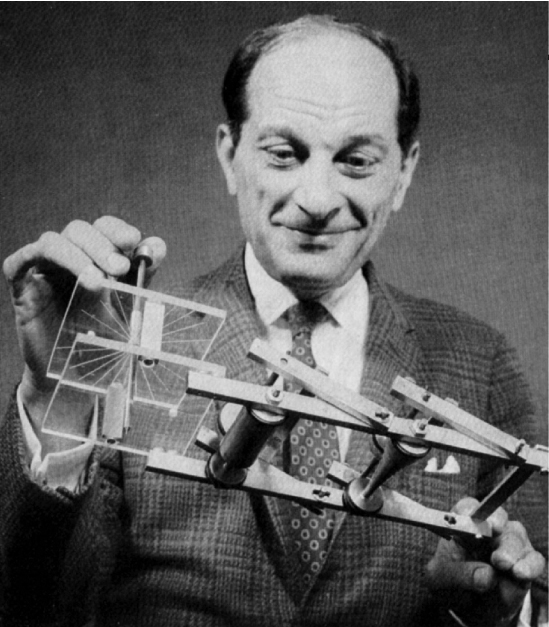
\includegraphics[width=0.9\columnwidth]{stanislaw.jpg}
		\end{column}
	\end{columns}
\end{frame}

\begin{frame}{History Behind the Monte Carlo Methods\footnote{those who are interested, should read \textcite{eckhardtStanUlamJohn1987}.}}
	\begin{columns}
		\begin{column}{0.8\textwidth}
			\begin{vfilleditems}
				\item The idea came when Ulam was playing Solitaire while recovering from surgery.
				Ulam was trying to calculate the deterministic, i.e. analytical solution,
				of the probability of being dealt an already-won game.
				The calculations where almost impossible.
				So, he thought that he could play hundreds of games to statistically estimate,
				i.e. numerical solution, the probability of this result.
				\item Ulam described the idea to John von Neumann in 1946.
				\item \small Due to the secrecy, von Neumann and Ulam's work demanded a code name.
				Nicholas Metropolis suggested using ``Monte Carlo'',
				a homage to the ``Casino Monte Carlo'' in Monaco,
				where Ulam's uncle would ask relatives for money to play.
			\end{vfilleditems}
		\end{column}
		\begin{column}{0.2\textwidth}
			\centering
			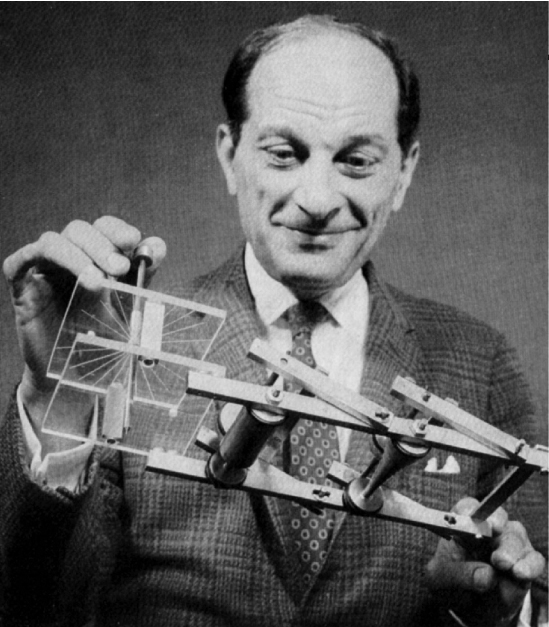
\includegraphics[width=0.9\columnwidth]{stanislaw.jpg}
		\end{column}
	\end{columns}
\end{frame}

\subsection{Why Do We Need MCMC?}
\begin{frame}{Why Do We Need MCMC?}
	The main computation barrier for Bayesian statistics is the denominator in Bayes' theorem,
	$P(\text{data})$:
	$$
		P(\theta \mid \text{data})=\frac{P(\theta) \cdot P(\text{data} \mid \theta)}{P(\text{data})}
	$$
	In discrete cases, we can turn the denominator into a sum over all parameters
	using the \textbf{chain rule} of probability:
	$$
		P(A,B \mid C)=P(A \mid B,C) \times P(B \mid C)
	$$
	This is also known as \textbf{marginalization}:
	$$
		P(\text{data})=\sum_{\theta} P(\text{data} \mid \theta) \times P(\theta)
	$$
\end{frame}

\begin{frame}{Why Do We Need MCMC?}
	However, in the case of continuous values,
	the denominator $P(\text{data})$
	turns into a very big and nasty integral:
	$$
		P(\text{data})=\int_{\theta} P(\text{data} \mid \theta) \times P(\theta)d \theta
	$$
	In many cases the integral is intractable
	(not possible of being deterministic evaluated) and,
	thus, we must find other ways to compute the posterior
	$P(\theta \mid \text{data})$ without using the denominator
	$P(\text{data})$.
	\vfill
	\Large \textbf{This is where Monte Carlo methods comes into play!}
\end{frame}

\begin{frame}{Why Do We Need the Denominator $P(\text{data})$?}
	To normalize the posterior with the intent of making it a \textbf{valid probability}.
	This means that the probability for all possible parameters' values must be $1$:
	\begin{vfilleditems}
		\item in the \textbf{discrete} case:
		$$
			\sum_{\theta} P(\theta \mid \text{data}) = 1
		$$
		\item in the \textbf{continuous} case:
		$$
			\int_{\theta} P(\theta \mid \text{data})d \theta = 1
		$$
	\end{vfilleditems}
\end{frame}

\begin{frame}{What If We Remove the Denominator $P(\text{data})$?}
	By removing the denominator $(\text{data})$,
	we conclude that the posterior
	$P(\theta \mid \text{data})$ is \textbf{proportional} to the
	product of the prior and the likelihood
	$P(\theta) \cdot P(\text{data} \mid \theta)$:
	$$
		P(\theta \mid \text{data}) \propto P(\theta) \cdot P(\text{data} \mid \theta)
	$$
\end{frame}

\subsubsection{Markov Chains}
\begin{frame}{Markov Chain Monte Carlo (MCMC)}
	Here is where \textbf{Markov Chain Monte Carlo} comes in:
	\vfill
	MCMC is an ample class of computational tools to approximate integrals
	and generate samples from a posterior probability
	\parencite{brooksHandbookMarkovChain2011}.
	\vfill
	MCMC is used when it is not possible to sample $\boldsymbol{\theta}$
	directly from the posterior probability
	$P(\boldsymbol{\theta} \mid \text{data})$.
	Instead, we collect samples in an iterative manner,
	where every step of the process we expect that the distribution which we are sampling from
	$P^*(\boldsymbol{\theta}^{(*)} \mid \text{data})$
	becomes more similar in every iteration to the posterior
	$P(\boldsymbol{\theta} \mid \text{data})$.
	\vfill
	All of this is to \textbf{eliminate the evaluation}
	(often impossible) of the \textbf{denominator}
	$P(\text{data})$.
\end{frame}

\begin{frame}{Markov Chains}
	\begin{columns}
		\begin{column}{0.8\textwidth}
			\begin{vfilleditems}
				\item We proceed by defining an \textbf{ergodic Markov chain}\footnote{
					meaning that there is an \textbf{unique stationary distribution}.}
				in which the set of possible states is the sample size and
				the stationary distribution is the distribution to be \textit{approximated}
				(or \textit{sampled}).
				\item Let $X_0, X_1, \dots, X_n$ be a simulation of the chain.
				The Markov chain \textbf{converges to the stationary distribution from any initial state}
				$X_0$ after a \textbf{sufficient large number of iterations} $r$.
				The distribution of the state $X_r$ will be similar to the stationary distribution,
				hence we can use it as a sample.
			\end{vfilleditems}
		\end{column}
		\begin{column}{0.2\textwidth}
			\centering
			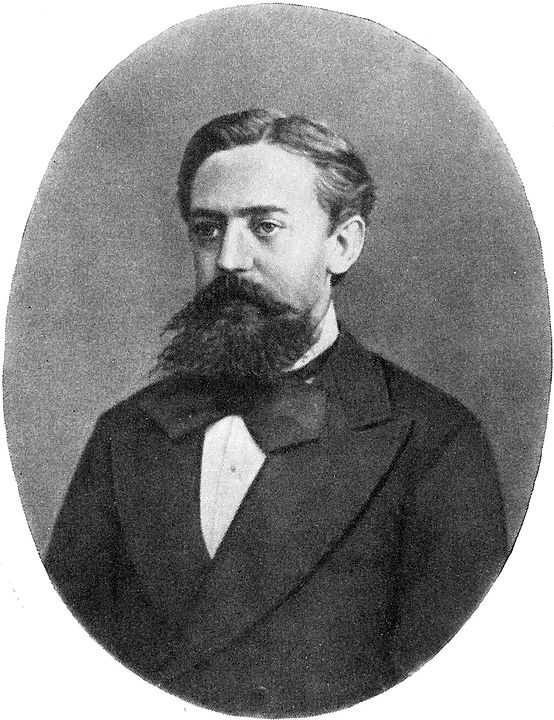
\includegraphics[width=0.9\columnwidth]{andrei_markov.jpg}
		\end{column}
	\end{columns}
\end{frame}

\begin{frame}{Markov Chains}
	\begin{columns}
		\begin{column}{0.8\textwidth}
			\begin{vfilleditems}
				\item Markov chains have a property that the probability distribution of the next state
				\textbf{depends only on the current state and not in the sequence of events that preceded}:
				$$
					P(X_{n+1}=x \mid X_{0},X_{1},X_{2},\ldots ,X_{n}) = P(X_{n+1}=x \mid X_{n})
				$$
				This property is called \textbf{Markovian}
				\item Similarly, using this argument with $X_r$ as the initial state,
				we can use $X_{2r}$ as a sample, and so on.
				We can use the sequence of states $X_r, X_{2r}, X_{3r}, \dots$
				as almost \textbf{independent samples} of Markov chain stationary distribution.
			\end{vfilleditems}
		\end{column}
		\begin{column}{0.2\textwidth}
			\centering
			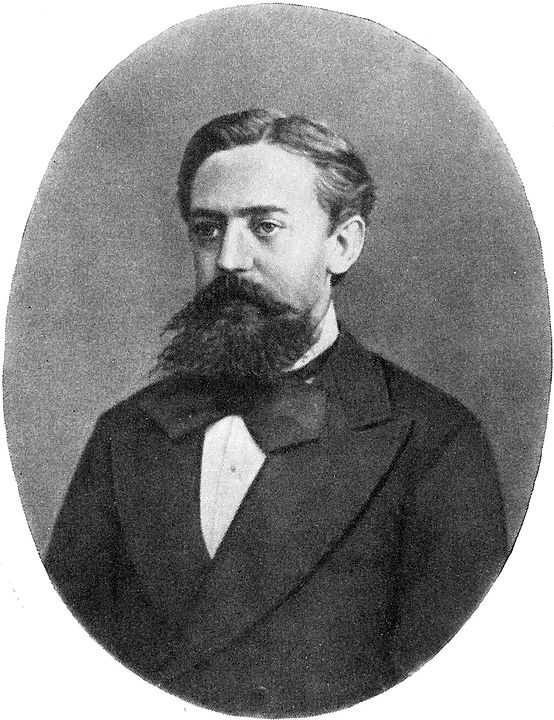
\includegraphics[width=0.9\columnwidth]{andrei_markov.jpg}
		\end{column}
	\end{columns}
\end{frame}

% Idea taken from http://steventhornton.ca/blog/markov-chains-in-latex.html
\begin{frame}{Example of a Markov Chain}
	\centering
	\begin{tikzpicture}
		% Add the states
		\node[state,
			text=yellow,
			minimum size=2cm,
			thick
		]
		(s) {Sun};
		\node[state,
			right=3cm of s,
			text=blue!30!white,
			minimum size=2cm,
			thick
		]
		(r) {Rain};

		% Connect the states with arrows
		\draw[every loop,
			auto=right,
			line width=1mm,
			>=latex]
		(s) edge[bend right, auto=left]  node {0.6} (r)
		(r) edge[bend right, auto=right] node {0.7} (s)
		(s) edge[loop above]             node {0.4} (s)
		(r) edge[loop above]             node {0.3} (r);
	\end{tikzpicture}
\end{frame}

\begin{frame}{Markov Chains}
	The efficacy of this approach depends on:
	\begin{vfilleditems}
		\item \textbf{how big $r$ must be} to guarantee an \textbf{adequate sample}.
		\item \textbf{computational power} required for every Markov chain iteration.
	\end{vfilleditems}

	\vfill
	\footnotesize
	Besides, it is custom to discard the first iterations of the algorithm because
	they are usually non-representative of the underlying stationary distribution to be approximate.
	In the initial iterations of MCMC algorithms,
	often the Markov chain is in a ``warm-up''\footnote{some references call this ``burnin''.} process,
	and its state is very far away from an ideal one to begin a trustworthy sampling.
	\vfill
	Generally, it is recommended to \textbf{discard the first half iterations} \parencite{gelmanBasicsMarkovChain2013}.
\end{frame}

\subsection{MCMC Algorithms}
\begin{frame}{MCMC Algorithms}
	We have \textbf{TONS} of MCMC algorithms\footnote{see the \href{https://en.wikipedia.org/wiki/Markov_chain_Monte_Carlo}
		{Wikipedia page for a full list}.}.
	Here we are going to cover two classes of MCMC algorithms:
	\begin{vfilleditems}
		\item Metropolis-Hastings \parencite{metropolisEquationStateCalculations1953, hastingsMonteCarloSampling1970}.

		\item Hamiltonian Monte Carlo\footnote{sometimes called Hybrid Monte Carlo, specially in the physics literature.} \parencite{neal2011mcmc, betancourtConceptualIntroductionHamiltonian2017}.
	\end{vfilleditems}
\end{frame}

\begin{frame}{MCMC Algorithms -- Metropolis-Hastings}
	These are the first MCMC algorithms.
	They use an \textbf{acceptance/rejection rule for the proposals}.
	They are characterized by proposals originated from a random walk in the parameter space.
	The \textbf{Gibbs algorithm} can be seen as a \textbf{special case} of MH
	because all proposals are automatically accepted \parencite{gelmanIterativeNonIterativeSimulation1992}
	\vfill
	Asymptotically, they have an acceptance rate of 23.4\%,
	and the computational cost of every iteration is $\mathcal{O}(d)$,
	where $d$ is the number of dimension in the parameter space \parencite{beskosOptimalTuningHybrid2013}.
\end{frame}

\begin{frame}{MCMC Algorithms -- Hamiltonian Monte Carlo}
	The current most efficient MCMC algorithms.
	They try to \textbf{avoid the random walk behavior by introducing an auxiliary vector of momenta
		using Hamiltonian dynamics}.
	The proposals are ``guided'' to higher density regions of the sample space.
	This makes \textbf{HMC more efficient in orders of magnitude when compared to MH and Gibbs}.
	\vfill
	Asymptotically, they have an acceptance rate of 65.1\%,
	and the computational cost of every iteration is $\mathcal{O}(d^{\frac{1}{4}})$,
	where $d$ is the number of dimension in the parameter space \parencite{beskosOptimalTuningHybrid2013}.
\end{frame}

\subsubsection{Metropolis}
\begin{frame}{Metropolis Algorithm}
	\begin{columns}
		\begin{column}{0.8\textwidth}
			The first broadly used MCMC algorithm to generate samples from a Markov chain
			was originated in the physics literature in the 1950s and is called Metropolis
			\parencite{metropolisEquationStateCalculations1953},
			in honor of the first author
			\href{https://en.wikipedia.org/wiki/Nicholas_Metropolis}{Nicholas Metropolis}.
			\vfill
			In sum, the Metropolis algorithm is an adaptation of a random walk coupled
			with an acceptance/rejection rule to converge to the target distribution.
			\vfill
			Metropolis algorithm uses a \textbf{proposal distribution}
			$J_t(\boldsymbol{\theta}^{(*)})$
			to define the next values of the distribution
			$P^*(\boldsymbol{\theta}^{(*)} \mid \text{data})$.
			This distribution must be symmetric:
			$$
				J_t (\boldsymbol{\theta}^{(*)} \mid \boldsymbol{\theta}^{(t-1)}) = J_t(\boldsymbol{\theta}^{(t-1)} \mid \boldsymbol{\theta}^{(*)})
			$$
		\end{column}
		\begin{column}{0.2\textwidth}
			\centering
			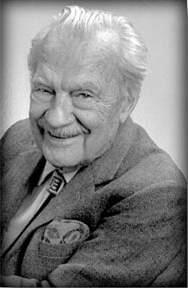
\includegraphics[width=0.9\columnwidth]{nicholas_metropolis.png}
		\end{column}
	\end{columns}
\end{frame}

\begin{frame}{Metropolis Algorithm}
	Metropolis is a random walk through the parameter sample space,
	where the probability of the Markov chain changing its state is defined as:
	$$
		P_{\text{change}} = \min\left({\frac{P (\boldsymbol{\theta}_{\text{proposed}})}{P (\boldsymbol{\theta}_{\text{current}})}},1\right).
	$$
	This means that the Markov chain will only change to a new state based in one of two conditions:
	\begin{vfilleditems}
		\small
		\item when the probability of the random walk proposed parameters
		$P(\boldsymbol{\theta}_{\text{proposed}})$ is \textbf{\textcolor{blue}{higher}}
		than the probability of the current state parameters
		$P(\boldsymbol{\theta}_{\text{current}})$,
		we change with 100\% probability.
		\item when the probability of the random walk proposed parameters
		$P(\boldsymbol{\theta}_{\text{proposed}})$ is \textbf{\textcolor{red}{lower}}
		than the probability of the current state parameters
		$P(\boldsymbol{\theta}_{\text{current}})$,
		we change with probability equal to the proportion of this probability difference.
	\end{vfilleditems}
\end{frame}

\begin{frame}{Metropolis Algorithm}
	\SetAlCapFnt{\normalsize}
	\SetAlCapNameFnt{\normalsize}
	\begin{algorithm}[H]
		\DontPrintSemicolon
		\SetAlgoNoEnd
		\SetAlgoLined
		Define an initial set $\boldsymbol{\theta}^{(0)} \in \mathbb{R}^p$ that $P\left(\boldsymbol{\theta}^{(0)} \mid \mathbf{y} \right) > 0$\;
		\For{$t = 1, 2, \dots$}{
			Sample a proposal of $\boldsymbol{\theta}^{(*)}$ from a proposal distribution in time $t$, $J_t \left(\boldsymbol{\theta}^{(*)} \mid \boldsymbol{\theta}^{(t-1)} \right)$\;
			As an acceptance/rejection rule, compute the proportion of the probabilities:
			$r = \frac{P\left(\boldsymbol{\theta}^{(*)}  \mid \mathbf{y} \right)}{P\left(\boldsymbol{\theta}^{(t-1)} \mid \mathbf{y} \right)}$\;
			Assign:
			$
				\boldsymbol{\theta}^{(t)} =
				\begin{cases}
					\boldsymbol{\theta}^{(*)}   & \text{with probability $\min(r,1)$} \\
					\boldsymbol{\theta}^{(t-1)} & \text{otherwise}
				\end{cases}
			$\;
		}
		\caption{Metropolis}
	\end{algorithm}
\end{frame}

\begin{frame}{Visual Intuition -- Metropolis}
	\centering
	\begin{tikzpicture}
		\begin{axis}[every axis plot, line width=2pt,
				ylabel=PDF,
				domain=-4:4,samples=200,
				ymax = 0.6, ytick={0, 0.2, 0.4},
				axis x line*=bottom, % no box around the plot, only x and y axis
				axis y line*=left, % the * suppresses the arrow tips
				enlargelimits=true,
			] % extend the axes a bit

			\addplot [blue] {gaussian(0, 1)};
			\node[inner sep=0pt] (hikerlower) at (-2,0.13){\Strichmaxerl[2pt]};
			\node[inner sep=0pt] (hikerupper) at (0,0.5){\Strichmaxerl[2pt]};
			\node[inner sep=0pt] (hikerlower2) at (2,0.13){\Strichmaxerl[2pt]};
			\draw[->, red, line width=2pt] (hikerlower) to [out=90,in=135] node[above left] {\large$P=1$} (hikerupper);
			\draw[->, yellow, line width=2pt] (hikerupper) to [out=45,in=135] node[right] {\large$P\approx\frac{0.1}{0.4}\approx\frac{1}{4}$} (hikerlower2);
		\end{axis}
	\end{tikzpicture}

\end{frame}

\subsubsection{Metropolis-Hastings (MH)}
\begin{frame}{Metropolis-Hastings Algorithm}
	\begin{columns}
		\begin{column}{0.8\textwidth}
			In the 1970s emerged a generalization of the Metropolis algorithm,
			which \textbf{does not need that the proposal distributions be symmetric}:
			$$
				J_t (\boldsymbol{\theta}^{(*)} \mid \boldsymbol{\theta}^{(t-1)}) \neq J_t(\boldsymbol{\theta}^{(t-1)} \mid \boldsymbol{\theta}^{(*)})
			$$
			The generalization was proposed by \href{https://en.wikipedia.org/wiki/W._K._Hastings}{Wilfred Keith Hastings}
			\parencite{hastingsMonteCarloSampling1970} and is called \textbf{Metropolis-Hastings algorithm}.
		\end{column}
		\begin{column}{0.2\textwidth}
			\centering
			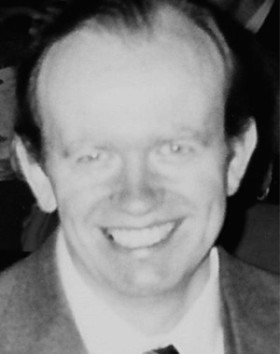
\includegraphics[width=0.9\columnwidth]{hastings.jpg}
		\end{column}
	\end{columns}
\end{frame}

\begin{frame}{Metropolis-Hastings Algorithm}
	\SetAlCapFnt{\normalsize}
	\SetAlCapNameFnt{\normalsize}
	\small
	\begin{algorithm}[H]
		\DontPrintSemicolon
		\SetAlgoNoEnd
		\SetAlgoLined
		Define an initial set $\boldsymbol{\theta}^{(0)} \in \mathbb{R}^p$ that $P\left(\boldsymbol{\theta}^{(0)} \mid \mathbf{y} \right) > 0$\;
		\For{$t = 1, 2, \dots$}{
			Sample a proposal $\boldsymbol{\theta}^{(*)}$ from a proposal distribution in time $t$, $J_t \left(\boldsymbol{\theta}^{(*)} \mid \boldsymbol{\theta}^{(t-1)} \right)$\;
			As an acceptance/rejection rule, compute the proportion of the probabilities:
			$r = \frac{\frac{P \left(\boldsymbol{\theta}^{(*)} \mid \mathbf{y} \right)}{J_t \left(\boldsymbol{\theta}^{(*)} \mid \boldsymbol{\theta}^{(t-1)} \right)}}{\frac{P \left(\boldsymbol{\theta}^{(t-1)} \mid \mathbf{y} \right)}{J_t \left(\boldsymbol{\theta}^{(t-1)} \mid \boldsymbol{\theta}^{(*)} \right)}}$\;
			Assign:
			$
				\boldsymbol{\theta}^{(t)} =
				\begin{cases}
					\boldsymbol{\theta}^{(*)}   & \text{with probability} \\
					\boldsymbol{\theta}^{(t-1)} & \text{otherwise}
				\end{cases}
			$\;
		}
		\caption{Metropolis-Hastings}
	\end{algorithm}
\end{frame}

\begin{frame}{Metropolis-Hastings Animation\footnote{see Metropolis-Hastings in action at \href{https://chi-feng.github.io/mcmc-demo/app.html?algorithm=RandomWalkMH&target=banana}{\texttt{chi-feng/mcmc-demo}}.}}
	\centering
	\movie[loop, width=9cm, height=6cm]{Metropolis Animation}{animations/rwmh.m4v}
\end{frame}

\subsubsection{Limitations of the Metropolis Algorithms}
\begin{frame}{Limitations of the Metropolis Algorithms}
	The limitations of the Metropolis-Hastings algorithms are mainly \textbf{computational}:
	\begin{vfilleditems}
		\item with the proposals randomly generated,
		it can take a large number of iterations for the
		Markov chain to enter higher posterior densities spaces.
		\item even highly-efficient MH algorithms sometimes accept less than
		25\% of the proposals \parencite{robertsWeakConvergenceOptimal1997, beskosOptimalTuningHybrid2013}.
		\item in lower-dimensional contexts, higher computational power can compensate the low efficiency up to a point.
		But in higher-dimensional (and higher-complexity) modeling situations,
		higher computational power alone are rarely sufficient to overcome the low efficiency.
	\end{vfilleditems}
\end{frame}

\subsubsection{Gibbs}
\begin{frame}{Gibbs Algorithm}
	\begin{columns}
		\begin{column}{0.8\textwidth}
			To circumvent Metropolis' low acceptance rate, the Gibbs algorithm was conceived.
			Gibbs \textbf{do not have an acceptance/rejection rule} for the Markov chain state change:
			\textbf{all proposals are accepted!}
			\vfill
			Gibbs algorithm was originally conceived by the physicist Josiah Willard Gibbs
			while referencing an analogy between a sampling algorithm and
			statistical physics (a physics field that originates from statistical mechanics).
			The algorithm was described by the Geman brothers in 1984
			\parencite{gemanStochasticRelaxationGibbs1984},
			about 8 decades after Gibbs death.
		\end{column}
		\begin{column}{0.2\textwidth}
			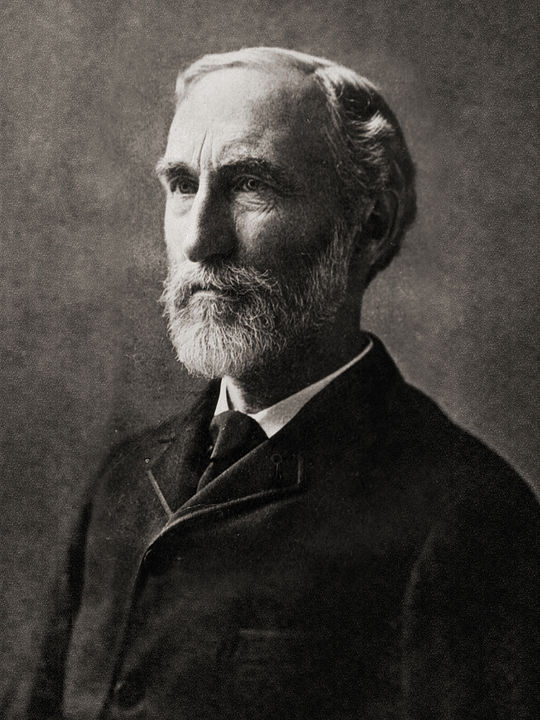
\includegraphics[width=0.9\columnwidth]{josiah_gibbs.jpg}
		\end{column}
	\end{columns}
\end{frame}

\begin{frame}{Gibbs Algorithm}
	The Gibbs algorithm is very useful in multidimensional sample spaces.
	It is also known as \textbf{alternating conditional sampling},
	because we always sample a parameter \textbf{conditioned} on the probability of the other model's parameters.
	\vfill
	The Gibbs algorithm can be seen as a \textbf{special case} of the Metropolis-Hastings algorithm,
	because all proposals are accepted
	\parencite{gelmanIterativeNonIterativeSimulation1992}.
	\vfill
	The essence of the Gibbs algorithm is the sampling of parameters conditioned in other parameters:
	$$P(\theta_1 \mid \theta_2, \dots \theta_p)$$
\end{frame}

\begin{frame}[fragile]{Gibbs Algorithm}
	\SetAlCapFnt{\normalsize}
	\SetAlCapNameFnt{\normalsize}
	\begin{algorithm}[H]
		\DontPrintSemicolon
		\SetAlgoNoEnd
		\SetAlgoLined
		Define an initial set $\boldsymbol{\theta}^{(0)} \in \mathbb{R}^p$ that $P\left(\boldsymbol{\theta}^{(0)} \mid \mathbf{y} \right) > 0$\;
		\For{$t = 1, 2, \dots$}{
			Assign:
			$ \boldsymbol{\theta}^{(t)} =
				\begin{cases}
					\theta^{(t)}_1 & \sim P \left(\theta_1 \mid \theta^{(0)}_2, \dots, \theta^{(0)}_p \right)         \\
					\theta^{(t)}_2 & \sim P \left(\theta_2 \mid \theta^{(t-1)}_1, \dots, \theta^{(0)}_p \right)       \\
					               & \vdots                                                                           \\
					\theta^{(t)}_p & \sim P \left(\theta_p \mid \theta^{(t-1)}_1, \dots, \theta^{(t-1)}_{p-1} \right)
				\end{cases}
			$\;
		}
		\caption{Gibbs}
	\end{algorithm}
\end{frame}

\begin{frame}{Gibbs Animation\footnote{see Gibbs in action at \href{https://chi-feng.github.io/mcmc-demo/app.html?algorithm=GibbsSampling&target=banana}{\texttt{chi-feng/mcmc-demo}}.}}
	\centering
	\movie[loop, width=9cm, height=6cm]{Gibbs Animation}{animations/gibbs.m4v}
\end{frame}

\subsubsection{Limitations of the Gibbs Algorithm}
\begin{frame}{Limitations of the Gibbs Algorithm}
	The main limitation of Gibbs algorithm is with relation to
	\textbf{alternating conditional sampling}:
	\begin{vfilleditems}
		\item In Metropolis, the parameters' random proposals are sampled
		\textbf{unconditionally}, \textbf{jointly}, and \textbf{simultaneous}.
		The Markov chain state changes are executed in a
		\textbf{multidimensional} manner.
		This makes \textbf{multidimensional diagonal movements}.
		\item In the case of the Gibbs algorithm,
		this movement only happens one parameter at a time,
		because we sample parameters in a
		\textbf{conditional} and \textbf{sequential} manner with respect
		to other parameters.
		This makes \textbf{unidimensional horizontal/vertical movements},
		and never multidimensional diagonal movements.
	\end{vfilleditems}
\end{frame}

\subsubsection{Hamiltonian Monte Carlo (HMC)}
\begin{frame}{Hamiltonian Monte Carlo (HMC)}
	\begin{columns}
		\begin{column}{0.8\textwidth}
			Metropolis' low acceptance rate and Gibbs' low performance in multidimensional problems
			(where the posterior geometry is highly complex)
			made a new class of MCMC algorithms to emerge.
			These are called Hamiltonian Monte Carlo (HMC),
			because they incorporate Hamiltonian dynamics
			(in honor of Irish physicist
			\href{https://en.wikipedia.org/wiki/William_Rowan_Hamilton}{William Rowan Hamilton}).
		\end{column}
		\begin{column}{0.2\textwidth}
			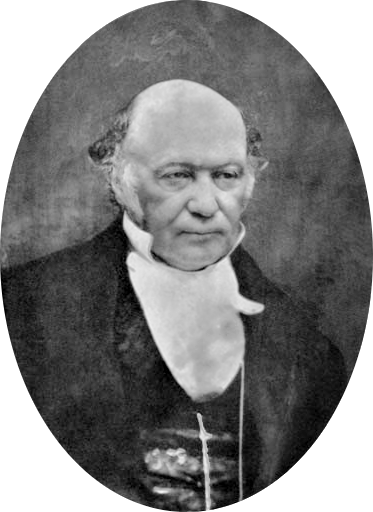
\includegraphics[width=0.9\columnwidth]{hamilton.png}
		\end{column}
	\end{columns}
\end{frame}

\begin{frame}{HMC Algorithm}
	HMC algorithm is an adaptation of the MH algorithm,
	and employs a guidance scheme to the generation of new proposals.
	It boosts the acceptance rate, and, consequently, has a better efficiency.
	\vfill
	More specifically, HMC uses the gradient of the posterior's log density
	to guide the Markov chain to higher density regions of the sample space,
	where most of the samples are sampled:
	$$
		\frac{d \log P(\boldsymbol{\theta} \mid \mathbf{y})}{d \theta}
	$$
	As a result, a Markov chain that uses a well-adjusted HMC algorithm will accept
	proposals with a much higher rate than if using the MH algorithm
	\parencite{robertsWeakConvergenceOptimal1997, beskosOptimalTuningHybrid2013}.
\end{frame}

\begin{frame}{History of HMC Algorithm}
	HMC was originally described in the physics literature\footnote{where is called ``Hybrid'' Monte Carlo (HMC)}
	\parencite{duaneHybridMonteCarlo1987}.
	\vfill
	Soon after, HMC was applied to statistical problems by
	\textcite{nealImprovedAcceptanceProcedure1994} who named it as Hamiltonian Monte Carlo (HMC).
	\vfill
	For a much more detailed and in-depth discussion (not our focus here) of HMC,
	I recommend
	\textcite{neal2011mcmc} and \textcite{betancourtConceptualIntroductionHamiltonian2017}.
\end{frame}

\begin{frame}{What Changes With HMC?}
	HMC uses Hamiltonian dynamics applied to particles efficiently exploring
	a posterior probability geometry,
	while also being robust to complex posterior's geometries.
	\vfill
	Besides that, HMC is much more efficiently than Metropolis and
	does \textit{not} suffer Gibbs' parameters correlation issues
\end{frame}

\begin{frame}{Intuition Behind the HMC Algorithm}
	\small
	For every parameter $\theta_j$, HMC adds a momentum variable $\phi_j$.
	The posterior density $P(\boldsymbol{\theta} \mid y)$ is incremented by an
	independent momenta distribution $P(\boldsymbol{\phi})$,
	hence defining the following joint probability:
	$$
		P(\boldsymbol{\theta}, \boldsymbol{\phi} \mid y) = P(\boldsymbol{\phi}) \cdot P(\boldsymbol{\theta} \mid y)
	$$
	\small
	HMC uses a proposal distribution that changes depending on the Markov chain current state.
	HMC finds the direction where the posterior density increases,
	the \textbf{gradient},
	and alters the proposal distribution towards the gradient direction.
	\vfill
	The probability of the Markov chain to change its state in HMC is defined as:
	$$
		P_{\text{change}} = \min\left({\frac{P(\boldsymbol{\theta}_{\text{proposed}}) \cdot P(\boldsymbol{\phi}_{\text{proposed}})}{P(\boldsymbol{\theta}_{\text{current}})\cdot P(\boldsymbol{\phi}_{\text{current}})}}, 1\right)
	$$
\end{frame}

\begin{frame}{Momenta Distribution -- $P(\boldsymbol{\phi})$}
	Generally we give $\boldsymbol{\phi}$ a multivariate normal distribution
	with mean $0$ and covariance$\mathbf{M}$,
	a ``mass matrix''.
	\vfill
	To keep things computationally simple,
	we used a \textbf{diagonal} mass matrix $\mathbf{M}$.
	This makes that the diagonal elements (components) $\boldsymbol{\phi}$ are independent,
	each one having a normal distribution:
	$$\phi_j \sim \text{Normal}(0, M_{jj})$$
\end{frame}

\begin{frame}[fragile]{HMC Algorithm}
	\SetAlCapFnt{\normalsize}
	\SetAlCapNameFnt{\normalsize}
	\begin{algorithm}[H]
		\DontPrintSemicolon
		\SetAlgoNoEnd
		\SetAlgoLined
		\footnotesize
		Define an initial set $\boldsymbol{\theta}^{(0)} \in \mathbb{R}^p$ that $P\left(\boldsymbol{\theta}^{(0)} \mid \mathbf{y} \right) > 0$\;
		Sample $\boldsymbol{\phi}$ from a $\text{Multivariate Normal}(\mathbf{0},\mathbf{M})$\;
		Simultaneously sample $\boldsymbol{\theta}^{(*)}$ and $\boldsymbol{\phi}$ with $L$ steps and step-size $\epsilon$.\;
		Define the current value of $\boldsymbol{\theta}$ as the proposed value $\boldsymbol{\theta}^{(*)}$:
		$\boldsymbol{\theta}^{(*)} \leftarrow \boldsymbol{\theta}$\;
		\For{$1, 2, \dots, L$}{
			Use the $\log$ of the posterior's gradient $\boldsymbol{\theta}^{(*)}$ to produce a half-step of $\boldsymbol{\phi}$:
			$\boldsymbol{\phi} \leftarrow \boldsymbol{\phi} + \frac{1}{2} \epsilon \frac{d \log P(\boldsymbol{\theta}^{(*)} \mid \mathbf{y})}{d \theta}$\;
			Use $\boldsymbol{\phi}$ to update $\boldsymbol{\theta}^{(*)}$:
			$\boldsymbol{\theta}^{(*)} \leftarrow \boldsymbol{\theta}^{(*)} + \epsilon \mathbf{M}^{-1} \boldsymbol{\phi}$\;
			Use again $\boldsymbol{\theta}^{(*)}$ $\log$ gradient to produce a half-step of $\boldsymbol{\phi}$:
			$\boldsymbol{\phi} \leftarrow \boldsymbol{\phi} + \frac{1}{2} \epsilon \frac{d \log P(\boldsymbol{\theta}^{(*)} \mid \mathbf{y})}{d \theta}$\;
		}
		As an acceptance/rejection rule, compute:
		$r = \frac{P \left(\boldsymbol{\theta}^{(*)} \mid \mathbf{y} \right) P \left(\boldsymbol{\phi}^{(*)} \right)}{P \left(\boldsymbol{\theta}^{(t-1)} \mid \mathbf{y} \right) P \left(\boldsymbol{\phi}^{(t-1)} \right)}$\;
		Assign:
		$
			\boldsymbol{\theta}^{(t)} =
			\begin{cases}
				\boldsymbol{\theta}^{(*)}   & \text{with probability $\min(r,1)$} \\
				\boldsymbol{\theta}^{(t-1)} & \text{otherwise}
			\end{cases}
		$\;
		\caption{Hamiltonian Monte Carlo (HMC)}
	\end{algorithm}
\end{frame}

\begin{frame}{HMC Animation\footnote{see HMC in action at \href{https://chi-feng.github.io/mcmc-demo/app.html?algorithm=HamiltonianHMC&target=banana}{\texttt{chi-feng/mcmc-demo}}.}}
	\centering
	\movie[loop, width=9cm, height=6cm]{HMC Animation}{animations/hmc.m4v}
\end{frame}

\begin{frame}{An Interlude into Numerical Integration}
	In the field of ordinary differential equations (ODE),
	we have the idea of ``discretizing'' a system of ODEs by applying a
	small step-size $\epsilon$\footnote{sometimes also called $h$}.
	Such approaches are called \textbf{numerical integrators} and are composed by
	an ample class of tools.
	\vfill
	The most famous and simple of these numerical integrators is the Euler method,
	where we use a step-size $\epsilon$ to compute a numerical solution of system
	in a future time $t$ from specific initial conditions.
\end{frame}

\begin{frame}{An Interlude into Numerical Integration}
	\begin{columns}
		\begin{column}{0.6\textwidth}
			The problem is that Euler method, when applied to Hamiltonian dynamics,
			\textbf{does not preserve volume}.
			One of the fundamental properties of Hamiltonian dynamics if
			\textbf{volume preservation}\footnote{a result called Liouville theorem.}.
			This makes the Euler method a bad choice as a HMC's numerical integrator.
		\end{column}
		\begin{column}{0.4\textwidth}
			\begin{figure}
				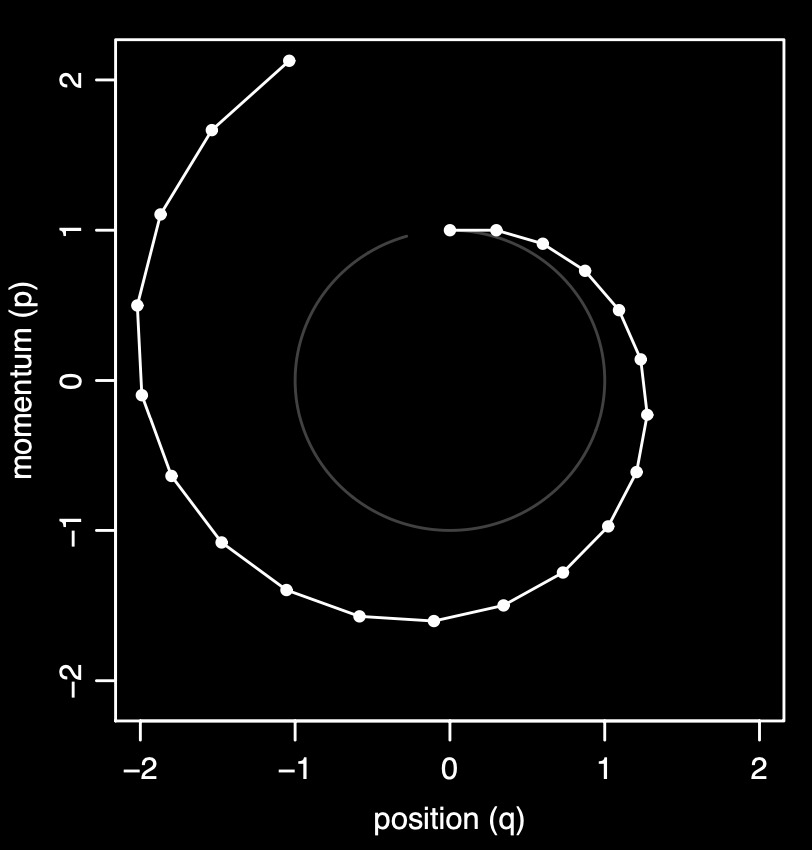
\includegraphics[width=0.8\columnwidth]{euler_0_3.jpg}
				\caption{HMC numerically integrated using Euler with $\epsilon = 0.3$ and $L = 20$}
			\end{figure}
		\end{column}
	\end{columns}
\end{frame}

\begin{frame}{An Interlude into Numerical Integration\footnote{
			An excellent textbook for numerical and symplectic integrator is
			\textcite{irseles2008numericalanalysis}.}}
	\begin{columns}
		\begin{column}{0.6\textwidth}
			To preserve volume, we need a numerical \textbf{symplectic integrator}.
			Symplectic integrators are at most second-order
			and demands a constant step-size $\epsilon$.
			One of the main numerical symplectic integrator used
			in Hamiltonian dynamics is the \textbf{Störmer–Verlet integrator},
			also known as \textbf{leapfrog integrator}.
		\end{column}
		\begin{column}{0.4\textwidth}
			\begin{figure}
				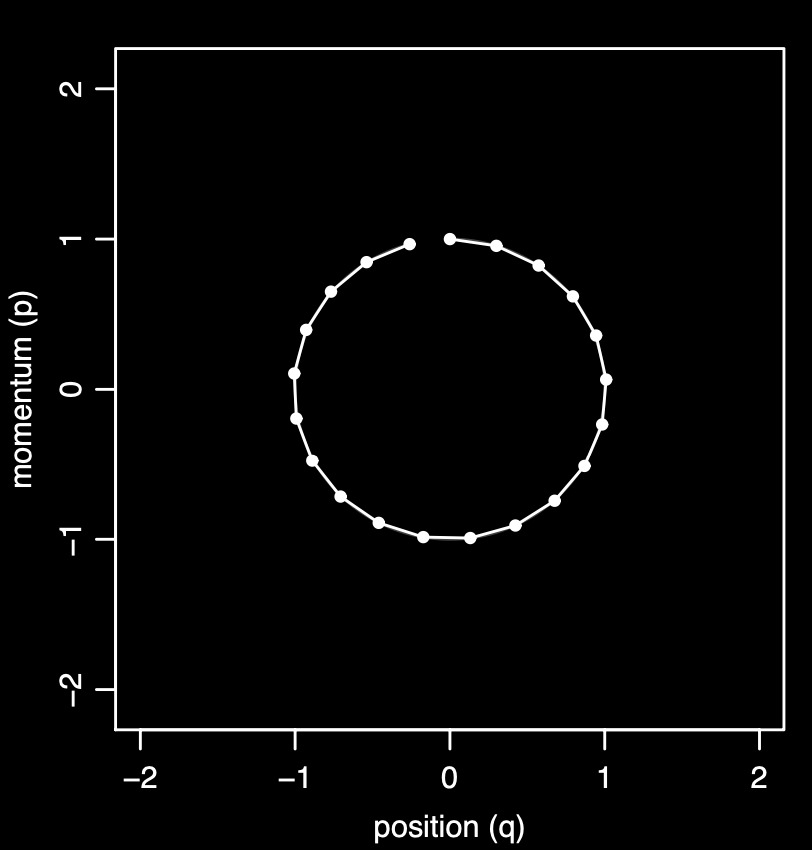
\includegraphics[width=0.8\columnwidth]{leapfrog_0_3.jpg}
				\caption{HMC numerically integrated using leapfrog with $\epsilon = 0.3$ and $L = 20$}
			\end{figure}
		\end{column}
	\end{columns}
\end{frame}

\begin{frame}{Limitations of the HMC Algorithm}
	\begin{columns}
		\begin{column}{0.6\textwidth}
			As you can see, HMC algorithm is highly sensible to the choice of
			leapfrog steps $L$ and step-size $\epsilon$,
			More specific, the leapfrog integrator allows only a constant $\epsilon$.
			There is a delicate balance between $L$ and $\epsilon$,
			that are hyperparameters and need to be carefully adjusted.
		\end{column}
		\begin{column}{0.4\textwidth}
			\begin{figure}
				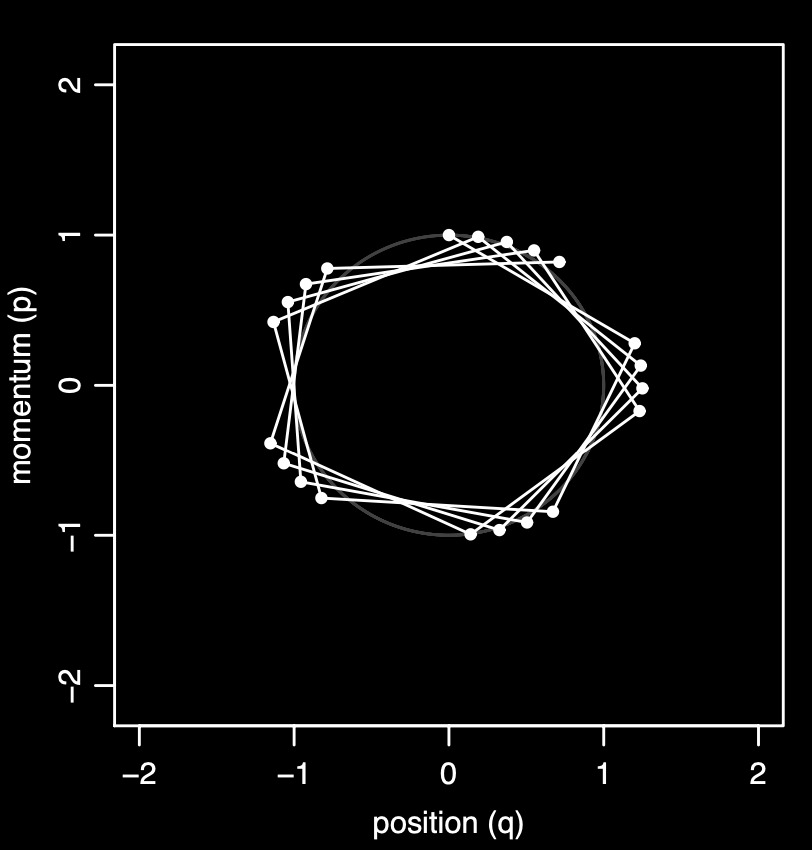
\includegraphics[width=0.8\columnwidth]{leapfrog_1_2.jpg}
				\caption{HMC numerically integrated using leapfrog with $\epsilon = 1.2$ and $L = 20$}
			\end{figure}
		\end{column}
	\end{columns}
\end{frame}

\subsubsection{No-U-Turn-Sampler (NUTS)}
\begin{frame}{\textbf{N}o-\textbf{U}-\textbf{T}urn-\textbf{S}ampler (NUTS)}
	In HMC, we can adjust $\epsilon$ during the algorithm runtime.
	But, for $L$, we need to to ``dry run'' the HMC sampler to find a good candidate value for $L$.
	\vfill
	Here is where the idea for \textbf{N}o-\textbf{U}-\textbf{T}urn-\textbf{S}ampler (NUTS)
	\parencite{hoffman2014no} enters:
	you don't need to \textbf{adjust anything},
	just ``press the button''.
	It will automatically find $\epsilon$ and $L$.
\end{frame}

\begin{frame}{\textbf{N}o-\textbf{U}-\textbf{T}urn-\textbf{S}ampler (NUTS)}
	More specifically, we need a criterion that informs that we performed
	enough Hamiltonian dynamics simulation.
	In other words, to simulate past beyond would not increase the distance
	between the proposal $\boldsymbol{\theta}^{(*)}$ and the current value $\boldsymbol{\theta}$.
	\vfill
	NUTS uses a criterion based on the dot product between the current momenta vector
	$\boldsymbol{\phi}$ and the difference between the proposal vector $\boldsymbol{\theta}^{(*)}$
	and the current vector $\boldsymbol{\theta}$,
	which turns into the derivative with respect to time $t$ of half of the distance squared between
	$\boldsymbol{\theta}$ e $\boldsymbol{\theta}^{(*)}$:
	$$
		(\boldsymbol{\theta}^{(*)} - \boldsymbol{\theta}) \cdot \boldsymbol{\phi}
		= (\boldsymbol{\theta}^{(*)} - \boldsymbol{\theta}) \cdot \frac{d}{dt} (\boldsymbol{\theta}^{(*)} - \boldsymbol{\theta})
		= \frac{d}{dt} \frac{(\boldsymbol{\theta}^{(*)} - \boldsymbol{\theta}) \cdot (\boldsymbol{\theta}^{(*)} - \boldsymbol{\theta})}{2}
	$$
\end{frame}

\begin{frame}{\textbf{N}o-\textbf{U}-\textbf{T}urn-\textbf{S}ampler (NUTS)}
	This suggests an algorithms that does not allow proposals be guided infinitely
	until the distance between the proposal $\boldsymbol{\theta}^{(*)}$ and the current
	$\boldsymbol{\theta}$ is less than zero.
	\vfill
	This means that such algorithm will \textbf{not allow u-turns}.
\end{frame}

\begin{frame}{\textbf{N}o-\textbf{U}-\textbf{T}urn-\textbf{S}ampler (NUTS)}
	NUTS uses the leapfrog integrator to create a binary tree where each leaf node
	is a proposal of the momenta vector $\boldsymbol{\phi}$ tracing both a forward
	($t+1$) as well as a backward ($t-1$) path in a determined fictitious time $t$.
	The growing of the leaf nodes are \textbf{interrupted} when an u-turn is detected,
	both forward or backward.
	\begin{figure}
		\centering
		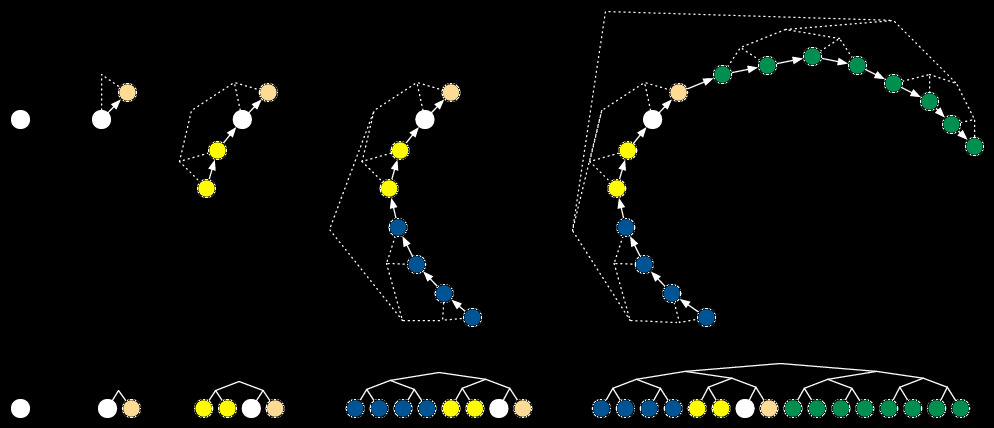
\includegraphics[width=0.6\textwidth]{nuts.jpg}
		\caption{NUTS growing leaf nodes forward}
	\end{figure}
\end{frame}

\begin{frame}{\textbf{N}o-\textbf{U}-\textbf{T}urn-\textbf{S}ampler (NUTS)}
	NUTS also uses a procedure called Dual Averaging
	\parencite{nesterov2009primal} to simultaneously adjust $\epsilon$ and $L$
	by considering the product $\epsilon \cdot L$.
	\vfill
	Such adjustment is done during the warmup phase and the defined values of
	$\epsilon$ and $L$ are kept fixed during the sampling phase.
\end{frame}

\begin{frame}{NUTS Algorithm}
	\SetAlCapFnt{\footnotesize}
	\SetAlCapNameFnt{\footnotesize}
	\begin{algorithm}[H]
		\DontPrintSemicolon
		\SetAlgoNoEnd
		\SetAlgoLined
		\fontsize{4.5pt}{6.5pt}\selectfont
		Define an initial set $\boldsymbol{\theta}^{(0)} \in \mathbb{R}^p$ that $P\left(\boldsymbol{\theta}^{(0)} \mid \mathbf{y} \right) > 0$\;
		\textcolor{blue}{Instantiate an empty binary tree with $2^L$ leaf nodes}\;
		Sample $\boldsymbol{\phi}$ from a $\text{Multivariate Normal}(\mathbf{0},\mathbf{M})$\;
		Simultaneously sample $\boldsymbol{\theta}$ and $\boldsymbol{\phi}$ with $L$ leapfrog steps and step-size $\epsilon$.\;
		Define the current value $\boldsymbol{\theta}$ as the proposed value $\boldsymbol{\theta}^{(*)}$:
		$\boldsymbol{\theta}^{(*)} \leftarrow \boldsymbol{\theta}$\;
		\For{$1, 2, \dots, 2L$}{
			\textcolor{blue}{Choose a direction $v \sim \text{Uniform}\left( \left\{-1, 1 \right\} \right)$}\;
			Use the gradient of the $\log$ posterior $\boldsymbol{\theta}^{(*)}$ for a half-step of $\boldsymbol{\phi}$ in the direction $v$:
			$\boldsymbol{\phi} \leftarrow \boldsymbol{\phi} + v \frac{1}{2} \epsilon \frac{d \log P(\boldsymbol{\theta}^{(*)} \mid \mathbf{y})}{d \theta}$\;
			Use $\boldsymbol{\phi}$ to update $\boldsymbol{\theta}^{(*)}$:
			$\boldsymbol{\theta}^{(*)} \leftarrow \boldsymbol{\theta}^{(*)} + \epsilon \mathbf{M}^{-1} \boldsymbol{\phi}$\;
			Again use the gradient of the $\log$ posterior $\boldsymbol{\theta}^{(*)}$ for a half-step of $\boldsymbol{\phi}$ in the direction $v$:
			$\boldsymbol{\phi} \leftarrow \boldsymbol{\phi} + v \frac{1}{2} \epsilon \frac{d \log P(\boldsymbol{\theta}^{(*)} \mid \mathbf{y})}{d \theta}$\;
			Define the node $L_t^v$ as the proposal $\boldsymbol{\theta}$\;
			\If{
				The difference between proposal vector $\boldsymbol{\theta}^{(*)}$
				and current vector $\boldsymbol{\theta}$ in the direction $v$ is lower than zero: $v \frac{d}{dt} \frac{(\boldsymbol{\theta}^{(*)} - \boldsymbol{\theta}^{(*)}) \cdot (\boldsymbol{\theta}^{(*)} - \boldsymbol{\theta}^{(*)})}{2} < 0$\;
			}{
				\textcolor{red}{Stop sampling $\boldsymbol{\theta}^{(*)}$ in the direction $v$ and continue sampling only in the direction $-v$}\;
			}{
				\If{
					The difference between proposal vector $\boldsymbol{\theta}^{(*)}$
					and current vector $\boldsymbol{\theta}$ in the direction $-v$ is lower than zero: $-v \frac{d}{dt} \frac{(\boldsymbol{\theta}^{(*)} - \boldsymbol{\theta}^{(*)}) \cdot (\boldsymbol{\theta}^{(*)} - \boldsymbol{\theta}^{(*)})}{2} < 0$\;
				}{
					\textcolor{red}{Stop sampling $\boldsymbol{\theta}^{(*)}$\;
					}
				}
			}
		}
		As an acceptance/rejection rule, compute:
		$r = \frac{P \left(\boldsymbol{\theta}^{(*)} \mid \mathbf{y} \right) P \left(\boldsymbol{\phi}^{(*)} \right)}{P \left(\boldsymbol{\theta}^{(t-1)} \mid \mathbf{y} \right) P \left(\boldsymbol{\phi}^{(t-1)} \right)}$\;
		Assign:
		$
			\boldsymbol{\theta}^{(t)} =
			\begin{cases}
				\boldsymbol{\theta}^{(*)}   & \text{with probability $\min(r,1)$} \\
				\boldsymbol{\theta}^{(t-1)} & \text{otherwise}
			\end{cases}
		$\;
		\caption{No-U-Turn-Sampler (NUTS)}
	\end{algorithm}
\end{frame}

\begin{frame}{NUTS Animation\footnote{see NUTS in action at \href{https://chi-feng.github.io/mcmc-demo/app.html?algorithm=EfficientNUTS&target=banana}{\texttt{chi-feng/mcmc-demo}}.}}
	\centering
	\movie[loop, width=9cm, height=6cm]{Animação NUTS}{animations/nuts.m4v}
\end{frame}

\subsubsection{Limitations of HMC and NUTS}
\begin{frame}{Limitations of HMC and NUTS Algorithms -- \textcite{nealSliceSampling2003}'s Funnel}
	The famous ``Devil's Funnel''\footnote{very common em hierarchical models.}.
	Here we see that HMC and NUTS, during the exploration of the posterior,
	have to change often $L$ and $\epsilon$ values\footnote{
		remember that $L$ and $\epsilon$ are defined in the warmup phase and kept fixed during sampling.}.
	% https://crackedbassoon.com/writing/funneling
	% import numpy as np
	% import matplotlib
	% import matplotlib.pyplot as plt
	% from matplotlib import rcParams
	% from scipy.stats import norm
	% fs = rcParams["figure.figsize"]
	% rcParams["figure.figsize"] = (fs[0], fs[0] / 2)
	% rcParams["lines.linewidth"] = 2
	% rcParams["font.size"] = 14
	% rcParams["axes.edgecolor"] = 'b'
	% rcParams["xtick.labelcolor"] = 'w'
	% rcParams["ytick.labelcolor"] = 'w'


	% # generate data
	% np.random.seed(0)
	% k = 9
	% n = 10000
	% v = norm.rvs(0, 3, n)
	% x = norm.rvs(0, np.exp(v / 2), (k, n))

	% # plot data and analytic log-likelihood
	% r = 500
	% x, v = np.meshgrid(np.linspace(-20, 20, r), np.linspace(-9, 9, r))
	% logp = norm.logpdf(v, 0, 3) + norm.logpdf(x, 0, np.exp(v / 2))
	% plt.imshow(logp, vmin=-7.5, vmax=-2.5, cmap="viridis", origin="lower")
	% plt.xticks(np.linspace(0, 499, 5), labels=np.linspace(-20, 20, 5).astype(int))
	% plt.yticks(np.linspace(0, 499, 5), labels=np.linspace(-9, 9, 5).astype(int))

	% # save figure
	% plt.savefig('slides/images/funnel.png', bbox_inches=0, transparent=True, dpi=300)
	\centering
	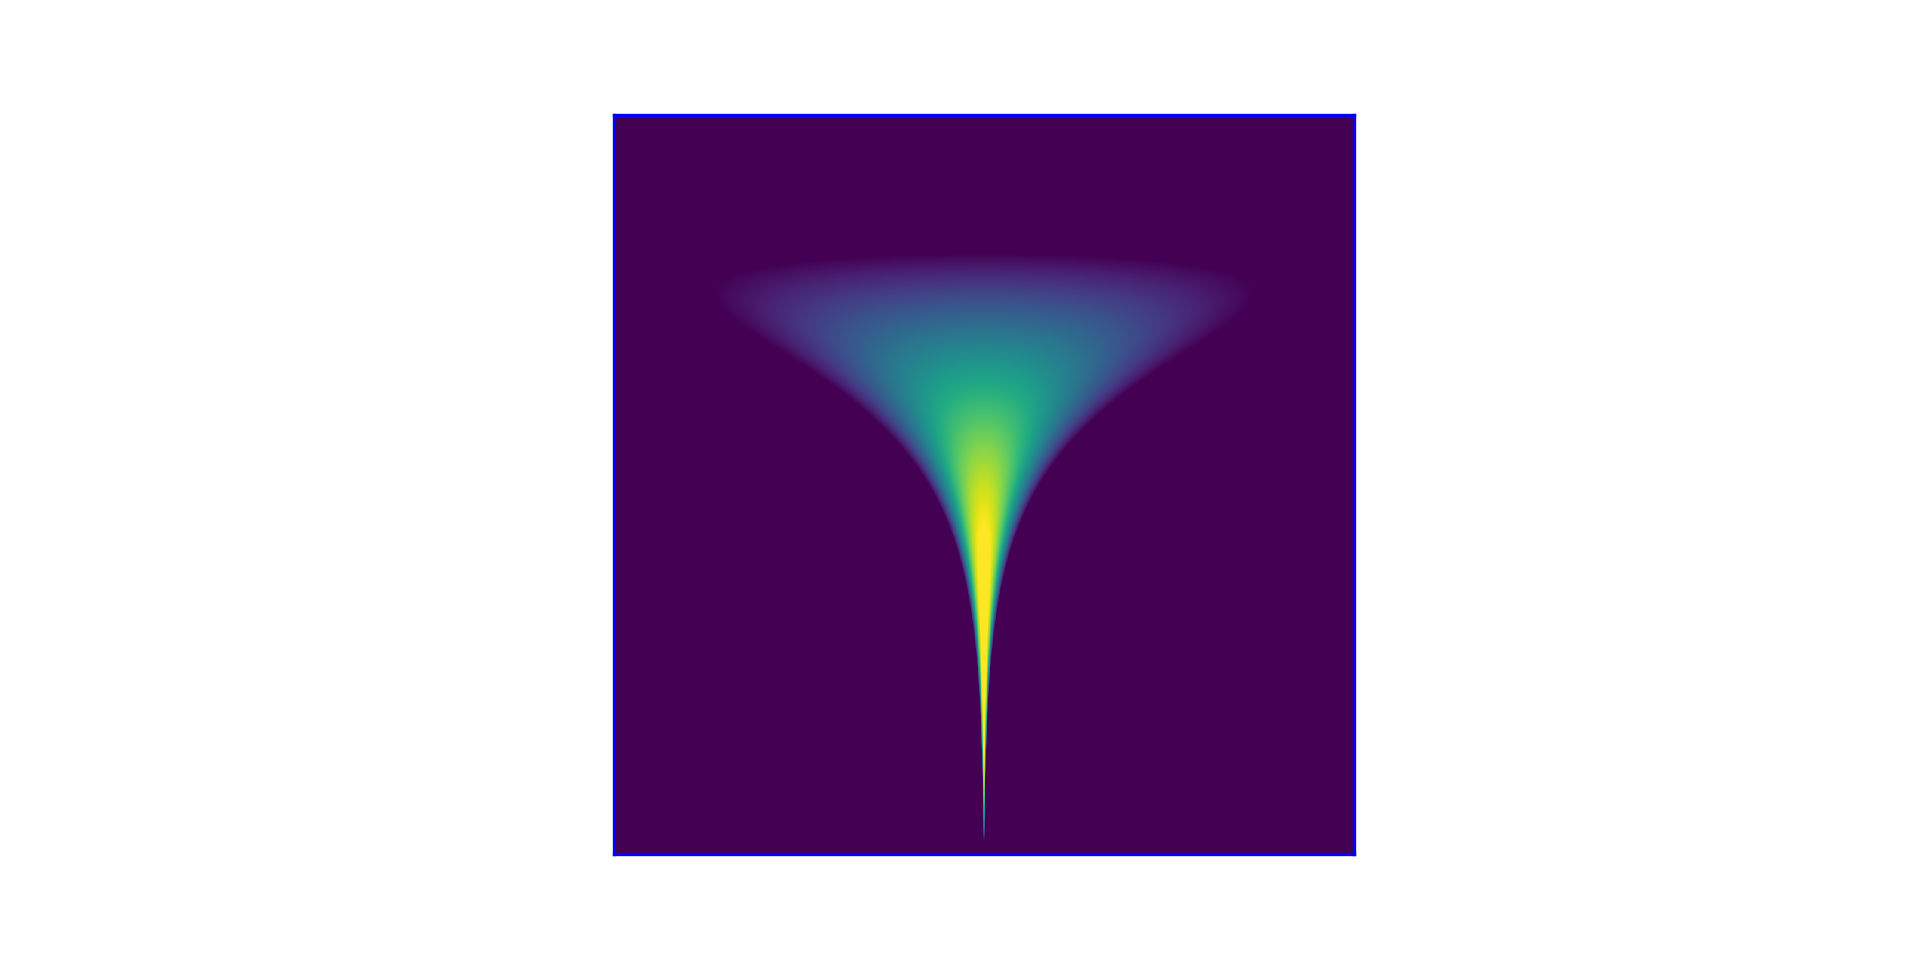
\includegraphics[width=0.65\textwidth]{funnel.png}
\end{frame}

\begin{frame}{\textcite{nealSliceSampling2003}'s Funnel and Non-Centered Parameterization (NCP)}
	Sometimes the group-level effects do not constrain the hierarchical distribution tightly.
	\vfill
	Examples arise when there are not many groups,
	or when the inter-group variation is high.
	\vfill
	In such cases, hierarchical models can be made much more efficient by shifting the
	data's correlation with the parameters to the hyperparameters.
\end{frame}

\begin{frame}{\textcite{nealSliceSampling2003}'s Funnel and Non-Centered Parameterization (NCP)}
	\small
	The funnel occurs when we have a variable that its variance depends on another variable variance
	in an exponential scale.
	A canonical example of a centered parameterization (CP) is:
	$$
		P(y,x) = \text{Normal}(y \mid 0 ,3) \cdot
		\text{Normal}\left(x \mid 0, e^{\left(\frac{y}{2}\right)}\right)
	$$
	This occurs often in hierarchical models,
	in the relationship between group-level priors and population-level hyperpriors.
	Hence, we reparameterize in a non-centered way,
	changing the posterior geometry to make life easier for our MCMC sampler:
	$$
		\begin{aligned}
			P(\tilde{y},\tilde{x}) & = \text{Normal}(\tilde{y} \mid 0, 1) \cdot
			\text{Normal}(\tilde{x} \mid 0, 1)                                           \\
			y                      & = \tilde{y} \cdot 3 + 0                             \\
			x                      & = \tilde{x} \cdot  e^{\left(\frac{y}{2}\right)} + 0
		\end{aligned}
	$$
\end{frame}

\begin{frame}{\texttt{Stan} and NUTS}
	\texttt{Stan} was the first MCMC sampler to implement NUTS.
	Besides that, it has an automatic optimized adjustment routine for values of $L$ and $\epsilon$ during warmup.
	It has the following default NUTS hyperparameters' values\footnote{
		for more information about how to change those values, see \href{
			https://mc-stan.org/docs/reference-manual/hmc-algorithm-parameters.html}{
			Section 15.2 of the \texttt{Stan} Reference Manual}.}:
	\begin{vfilleditems}
		\item \textbf{target acceptance rate of Metropolis proposals}: 0.8
		\item \textbf{max tree depth} (in powers of $2$): 10 (which means $2^{10} = 1024$)
	\end{vfilleditems}
\end{frame}

\begin{frame}{\texttt{Turing.jl} and NUTS}
	\texttt{Turing.jl} also implements NUTS which lives, along with other MCMC samplers, inside the package \texttt{AdvancedHMC.jl}.
	It also has an automatic optimized adjustment routine for values of $L$ and $\epsilon$ during warmup.
	It has the same default NUTS hyperparameters' values\footnote{
		for more information about how to change those values, see \href{
			https://turing.ml/dev/docs/library}{
			\texttt{Turing.jl} Documentation}.}:
	\begin{vfilleditems}
		\item \textbf{target acceptance rate of Metropolis proposals}: 0.65
		\item \textbf{max tree depth} (in powers of $2$): 10 (which means $2^{10} = 1024$)
	\end{vfilleditems}
\end{frame}

\subsection{Markov Chain Convergence}
\begin{frame}{Markov Chain Convergence}
	MCMC has an interesting property that it will
	\textbf{asymptotically converge to the target distribution}\footnote{
		this property is not present on neural networks.}.
	\vfill
	That means, if we have all the time in the world, it is guaranteed,
	irrelevant of the target distribution posterior geometry,
	\textbf{MCMC will give you the right answer}.
	\vfill
	However, we don't have all the time in the world
	Different MCMC algorithms, like HMC and NUTS,
	can reduce the sampling (and warmup) time necessary for convergence to the target distribution.
\end{frame}

\subsubsection{Convergence Metrics}
\begin{frame}{Convergence Metrics}
	We have some options on how to measure if the Markov chains converged to the target distribution,
	i.e. if they are ``reliable'':
	\begin{vfilleditems}
		\item \textbf{Effective Sample Size} (ESS):
		an approximation of the ``number of independent samples'' generated by a Markov chain.
		\item $\widehat{R}$ (\textbf{Rhat}):
		potential scale reduction factor,
		a metric to measure if the Markov chain have mixed,
		and, potentially, converged.
	\end{vfilleditems}
\end{frame}

\begin{frame}{Convergence Metrics -- Effective Sample Size \parencite{gelman2013bayesian}}
	$$\widehat{n}_{\text{eff}} = \frac{mn}{1 + \sum_{t=1}^T \widehat{\rho}_t}$$
	Where:
	\begin{vfilleditems}
		\item $m$: number of Markov chains.
		\item $n$: total samples per Markov chain (discarding warmup).
		\item $\widehat{\rho}_t$: an autocorrelation estimate.
	\end{vfilleditems}
\end{frame}

\begin{frame}{Convergence Metrics -- Rhat \parencite{gelman2013bayesian}}
	$$\widehat{R} = \sqrt{\frac{\widehat{\text{var}}^+(\psi \mid y)}{W}}$$
	where $\widehat{\text{var}}^+(\psi \mid y)$ is the Markov chains' sample variance
	for a certain parameter $\psi$.
	We calculate it by using a weighted sum of the within-chain $W$
	and between-chain $B$ variances:
	$$\widehat{\text{var}}^+(\psi \mid y) = \frac{n-1}{n} W + \frac{1}{n} B$$
	\vfill
	Intuitively, the value is $1.0$ if all chains are totally convergent.
	As a heuristic, if $\widehat{R} > 1.1$,
	you need to worry because probably the chains have not converged adequate.
\end{frame}

\subsubsection{Convergence Visualizations}
% plots taken from script:
% slides/images/bad_chains_traceplot.tex
\begin{frame}{Traceplot -- Convergent Markov Chains}
	\begin{figure}
		\centering
		\resizebox{.4\linewidth}{!}{% Created by tikzDevice version 0.12.3.1 on 2021-05-31 11:59:55
% !TEX encoding = UTF-8 Unicode
\begin{tikzpicture}[x=1pt,y=1pt]
\definecolor{fillColor}{RGB}{255,255,255}
\path[use as bounding box,fill=fillColor,fill opacity=0.00] (0,0) rectangle (505.89,505.89);
\begin{scope}
\path[clip] (  0.00,  0.00) rectangle (505.89,505.89);
\definecolor{drawColor}{RGB}{0,0,0}
\definecolor{fillColor}{RGB}{0,0,0}

\path[draw=drawColor,line width= 0.6pt,line join=round,line cap=round,fill=fillColor] (  0.00,  0.00) rectangle (505.89,505.89);
\end{scope}
\begin{scope}
\path[clip] ( 22.18, 18.22) rectangle (449.67,500.39);
\definecolor{fillColor}{RGB}{0,0,0}

\path[fill=fillColor] ( 22.18, 18.22) rectangle (449.67,500.39);
\definecolor{drawColor}{gray}{0.13}

\path[draw=drawColor,line width= 0.1pt,line join=round] ( 22.18, 76.16) --
	(449.67, 76.16);

\path[draw=drawColor,line width= 0.1pt,line join=round] ( 22.18,171.51) --
	(449.67,171.51);

\path[draw=drawColor,line width= 0.1pt,line join=round] ( 22.18,266.86) --
	(449.67,266.86);

\path[draw=drawColor,line width= 0.1pt,line join=round] ( 22.18,362.20) --
	(449.67,362.20);

\path[draw=drawColor,line width= 0.1pt,line join=round] ( 22.18,457.55) --
	(449.67,457.55);

\path[draw=drawColor,line width= 0.1pt,line join=round] ( 84.36, 18.22) --
	( 84.36,500.39);

\path[draw=drawColor,line width= 0.1pt,line join=round] (170.72, 18.22) --
	(170.72,500.39);

\path[draw=drawColor,line width= 0.1pt,line join=round] (257.09, 18.22) --
	(257.09,500.39);

\path[draw=drawColor,line width= 0.1pt,line join=round] (343.45, 18.22) --
	(343.45,500.39);

\path[draw=drawColor,line width= 0.1pt,line join=round] (429.81, 18.22) --
	(429.81,500.39);

\path[draw=drawColor,line width= 0.3pt,line join=round] ( 22.18, 28.49) --
	(449.67, 28.49);

\path[draw=drawColor,line width= 0.3pt,line join=round] ( 22.18,123.84) --
	(449.67,123.84);

\path[draw=drawColor,line width= 0.3pt,line join=round] ( 22.18,219.18) --
	(449.67,219.18);

\path[draw=drawColor,line width= 0.3pt,line join=round] ( 22.18,314.53) --
	(449.67,314.53);

\path[draw=drawColor,line width= 0.3pt,line join=round] ( 22.18,409.88) --
	(449.67,409.88);

\path[draw=drawColor,line width= 0.3pt,line join=round] ( 41.18, 18.22) --
	( 41.18,500.39);

\path[draw=drawColor,line width= 0.3pt,line join=round] (127.54, 18.22) --
	(127.54,500.39);

\path[draw=drawColor,line width= 0.3pt,line join=round] (213.91, 18.22) --
	(213.91,500.39);

\path[draw=drawColor,line width= 0.3pt,line join=round] (300.27, 18.22) --
	(300.27,500.39);

\path[draw=drawColor,line width= 0.3pt,line join=round] (386.63, 18.22) --
	(386.63,500.39);
\definecolor{drawColor}{RGB}{1,31,75}

\path[draw=drawColor,line width= 0.4pt,line join=round] ( 41.61,222.92) --
	( 42.04,204.96) --
	( 42.48,206.25) --
	( 42.91,165.69) --
	( 43.34,165.69) --
	( 43.77,163.58) --
	( 44.20,221.08) --
	( 44.63,210.00) --
	( 45.07,275.91) --
	( 45.50,136.32) --
	( 45.93,248.08) --
	( 46.36,228.21) --
	( 46.79,218.61) --
	( 47.23,245.67) --
	( 47.66,213.48) --
	( 48.09,255.03) --
	( 48.52,158.23) --
	( 48.95,299.50) --
	( 49.38,341.55) --
	( 49.82,283.34) --
	( 50.25,283.34) --
	( 50.68,118.63) --
	( 51.11,204.07) --
	( 51.54,217.46) --
	( 51.98,247.07) --
	( 52.41,165.21) --
	( 52.84,165.58) --
	( 53.27,244.06) --
	( 53.70,170.69) --
	( 54.13,217.63) --
	( 54.57,225.28) --
	( 55.00,221.31) --
	( 55.43,189.70) --
	( 55.86,170.14) --
	( 56.29,251.82) --
	( 56.73,241.96) --
	( 57.16,197.19) --
	( 57.59,290.64) --
	( 58.02,228.73) --
	( 58.45,298.48) --
	( 58.88,202.02) --
	( 59.32,187.21) --
	( 59.75,167.25) --
	( 60.18,185.49) --
	( 60.61,185.49) --
	( 61.04,209.39) --
	( 61.48,249.73) --
	( 61.91,229.47) --
	( 62.34,229.47) --
	( 62.77,207.24) --
	( 63.20,145.54) --
	( 63.63,251.30) --
	( 64.07,246.69) --
	( 64.50,246.69) --
	( 64.93,246.69) --
	( 65.36,226.98) --
	( 65.79,158.71) --
	( 66.23,226.74) --
	( 66.66,228.86) --
	( 67.09,219.07) --
	( 67.52,271.03) --
	( 67.95,236.38) --
	( 68.38,247.12) --
	( 68.82,207.82) --
	( 69.25,176.18) --
	( 69.68,267.48) --
	( 70.11,179.57) --
	( 70.54,295.11) --
	( 70.98,205.16) --
	( 71.41,231.62) --
	( 71.84,231.62) --
	( 72.27,240.95) --
	( 72.70,240.95) --
	( 73.13,196.06) --
	( 73.57,190.89) --
	( 74.00,190.89) --
	( 74.43,227.82) --
	( 74.86,203.44) --
	( 75.29,203.44) --
	( 75.73,259.20) --
	( 76.16,134.68) --
	( 76.59,265.00) --
	( 77.02,145.18) --
	( 77.45,265.84) --
	( 77.88,168.13) --
	( 78.32,310.48) --
	( 78.75,108.72) --
	( 79.18,298.87) --
	( 79.61,348.38) --
	( 80.04,302.02) --
	( 80.48,182.41) --
	( 80.91,299.84) --
	( 81.34,294.94) --
	( 81.77,200.94) --
	( 82.20,261.79) --
	( 82.63,282.66) --
	( 83.07,258.84) --
	( 83.50,174.13) --
	( 83.93,123.91) --
	( 84.36,123.91) --
	( 84.79,177.59) --
	( 85.23,267.42) --
	( 85.66,225.41) --
	( 86.09,225.87) --
	( 86.52,155.73) --
	( 86.95,223.15) --
	( 87.38,292.38) --
	( 87.82,165.90) --
	( 88.25,293.99) --
	( 88.68,111.82) --
	( 89.11,308.27) --
	( 89.54,192.52) --
	( 89.98,216.75) --
	( 90.41,233.78) --
	( 90.84,336.24) --
	( 91.27,257.34) --
	( 91.70,223.61) --
	( 92.13,237.18) --
	( 92.57,195.07) --
	( 93.00,189.85) --
	( 93.43,223.60) --
	( 93.86,198.09) --
	( 94.29,199.33) --
	( 94.72,254.04) --
	( 95.16,254.04) --
	( 95.59,109.19) --
	( 96.02,307.88) --
	( 96.45,144.58) --
	( 96.88,176.90) --
	( 97.32,267.32) --
	( 97.75,209.88) --
	( 98.18,230.93) --
	( 98.61,159.53) --
	( 99.04,310.33) --
	( 99.47,164.82) --
	( 99.91,264.89) --
	(100.34,261.06) --
	(100.77,326.53) --
	(101.20,122.36) --
	(101.63,308.11) --
	(102.07,212.60) --
	(102.50,266.07) --
	(102.93,260.38) --
	(103.36,156.96) --
	(103.79,272.85) --
	(104.22,272.85) --
	(104.66,176.68) --
	(105.09,289.38) --
	(105.52,105.81) --
	(105.95,302.47) --
	(106.38,272.05) --
	(106.82,306.64) --
	(107.25,306.64) --
	(107.68,169.46) --
	(108.11,196.34) --
	(108.54,162.32) --
	(108.97,283.98) --
	(109.41,252.06) --
	(109.84,185.97) --
	(110.27,260.11) --
	(110.70,119.57) --
	(111.13,165.42) --
	(111.57,190.26) --
	(112.00,260.97) --
	(112.43,264.92) --
	(112.86,192.31) --
	(113.29,192.31) --
	(113.72,251.86) --
	(114.16,212.46) --
	(114.59,210.38) --
	(115.02,236.67) --
	(115.45,253.40) --
	(115.88,268.63) --
	(116.32,294.83) --
	(116.75, 97.84) --
	(117.18,107.08) --
	(117.61,183.53) --
	(118.04,250.33) --
	(118.47,284.46) --
	(118.91,207.24) --
	(119.34,287.32) --
	(119.77,276.65) --
	(120.20,169.57) --
	(120.63,158.92) --
	(121.07,188.43) --
	(121.50,215.85) --
	(121.93,266.11) --
	(122.36,155.30) --
	(122.79,284.70) --
	(123.22,115.02) --
	(123.66,311.31) --
	(124.09,131.66) --
	(124.52,146.35) --
	(124.95,288.28) --
	(125.38,291.99) --
	(125.82,308.56) --
	(126.25,210.54) --
	(126.68,182.48) --
	(127.11,230.44) --
	(127.54,206.43) --
	(127.97,209.22) --
	(128.41,151.90) --
	(128.84,270.42) --
	(129.27,172.92) --
	(129.70,269.16) --
	(130.13,161.18) --
	(130.57,219.84) --
	(131.00,267.06) --
	(131.43,267.06) --
	(131.86,267.06) --
	(132.29,394.56) --
	(132.72,162.09) --
	(133.16,320.31) --
	(133.59,322.13) --
	(134.02,332.88) --
	(134.45,127.98) --
	(134.88,130.69) --
	(135.32,272.58) --
	(135.75,338.32) --
	(136.18,259.09) --
	(136.61,212.76) --
	(137.04,154.32) --
	(137.47,147.11) --
	(137.91,147.11) --
	(138.34,316.23) --
	(138.77,316.23) --
	(139.20,174.68) --
	(139.63,275.28) --
	(140.07,245.70) --
	(140.50,225.62) --
	(140.93,225.62) --
	(141.36,160.81) --
	(141.79,211.09) --
	(142.22,201.63) --
	(142.66,201.63) --
	(143.09,203.07) --
	(143.52,160.90) --
	(143.95,158.15) --
	(144.38,240.01) --
	(144.82,208.37) --
	(145.25,323.11) --
	(145.68,218.63) --
	(146.11,228.25) --
	(146.54,235.61) --
	(146.97,195.45) --
	(147.41,241.57) --
	(147.84,238.44) --
	(148.27,194.05) --
	(148.70,238.79) --
	(149.13,304.87) --
	(149.57,304.87) --
	(150.00,154.25) --
	(150.43,295.19) --
	(150.86,214.66) --
	(151.29,185.17) --
	(151.72,247.93) --
	(152.16,204.36) --
	(152.59,349.52) --
	(153.02,131.11) --
	(153.45,247.59) --
	(153.88,298.77) --
	(154.32,192.19) --
	(154.75,232.17) --
	(155.18,179.93) --
	(155.61,232.53) --
	(156.04,244.37) --
	(156.47,233.66) --
	(156.91,260.53) --
	(157.34,176.14) --
	(157.77,192.72) --
	(158.20,234.69) --
	(158.63,216.74) --
	(159.07,216.74) --
	(159.50,236.61) --
	(159.93,236.61) --
	(160.36,236.61) --
	(160.79,204.45) --
	(161.22,235.53) --
	(161.66,235.53) --
	(162.09,243.95) --
	(162.52,152.44) --
	(162.95,199.80) --
	(163.38,220.79) --
	(163.81,242.29) --
	(164.25,277.88) --
	(164.68,300.31) --
	(165.11,211.07) --
	(165.54,268.21) --
	(165.97,268.21) --
	(166.41,268.21) --
	(166.84,165.59) --
	(167.27,282.95) --
	(167.70,184.84) --
	(168.13,202.35) --
	(168.56,202.35) --
	(169.00,202.35) --
	(169.43,204.21) --
	(169.86,212.66) --
	(170.29,203.46) --
	(170.72,162.25) --
	(171.16,269.40) --
	(171.59,154.24) --
	(172.02,271.32) --
	(172.45,132.51) --
	(172.88,132.51) --
	(173.31,334.59) --
	(173.75,102.61) --
	(174.18,101.20) --
	(174.61,149.64) --
	(175.04,250.80) --
	(175.47,245.24) --
	(175.91,173.38) --
	(176.34,135.21) --
	(176.77,135.21) --
	(177.20,159.79) --
	(177.63,261.28) --
	(178.06,259.53) --
	(178.50,183.64) --
	(178.93,255.55) --
	(179.36,255.55) --
	(179.79,287.98) --
	(180.22,152.39) --
	(180.66,224.90) --
	(181.09,197.18) --
	(181.52,262.95) --
	(181.95,229.53) --
	(182.38,254.11) --
	(182.81,254.11) --
	(183.25,235.41) --
	(183.68,224.39) --
	(184.11,232.92) --
	(184.54, 74.82) --
	(184.97,347.62) --
	(185.41,168.41) --
	(185.84,166.59) --
	(186.27,236.73) --
	(186.70,236.73) --
	(187.13,214.30) --
	(187.56,285.52) --
	(188.00,173.92) --
	(188.43,235.52) --
	(188.86,146.72) --
	(189.29,302.12) --
	(189.72,345.93) --
	(190.16,113.05) --
	(190.59,283.45) --
	(191.02,175.61) --
	(191.45,233.57) --
	(191.88,263.54) --
	(192.31,273.09) --
	(192.75,123.35) --
	(193.18,277.14) --
	(193.61,152.00) --
	(194.04,261.74) --
	(194.47,238.10) --
	(194.91,178.76) --
	(195.34,283.52) --
	(195.77,230.76) --
	(196.20,325.23) --
	(196.63,325.23) --
	(197.06,298.16) --
	(197.50,275.75) --
	(197.93,176.93) --
	(198.36,203.33) --
	(198.79,203.33) --
	(199.22,130.22) --
	(199.66,257.99) --
	(200.09,257.99) --
	(200.52,190.68) --
	(200.95,215.00) --
	(201.38,255.58) --
	(201.81,226.40) --
	(202.25,209.04) --
	(202.68,166.48) --
	(203.11,226.76) --
	(203.54,234.61) --
	(203.97,170.36) --
	(204.41,271.08) --
	(204.84,271.08) --
	(205.27,166.11) --
	(205.70,154.54) --
	(206.13,228.03) --
	(206.56,228.03) --
	(207.00,328.11) --
	(207.43,267.36) --
	(207.86,248.84) --
	(208.29,159.32) --
	(208.72,277.74) --
	(209.16,159.95) --
	(209.59,259.92) --
	(210.02,251.69) --
	(210.45,176.92) --
	(210.88, 88.49) --
	(211.31,326.99) --
	(211.75,302.15) --
	(212.18,130.73) --
	(212.61,122.77) --
	(213.04,231.55) --
	(213.47,298.38) --
	(213.91,208.92) --
	(214.34,183.21) --
	(214.77,266.11) --
	(215.20,328.92) --
	(215.63,275.58) --
	(216.06,228.15) --
	(216.50,190.04) --
	(216.93,337.48) --
	(217.36,237.22) --
	(217.79,235.90) --
	(218.22,235.90) --
	(218.66,250.22) --
	(219.09,195.27) --
	(219.52,269.65) --
	(219.95,234.71) --
	(220.38,135.94) --
	(220.81,216.79) --
	(221.25,216.79) --
	(221.68,146.71) --
	(222.11,187.27) --
	(222.54,190.58) --
	(222.97,199.96) --
	(223.41,191.56) --
	(223.84,190.99) --
	(224.27,259.67) --
	(224.70,168.18) --
	(225.13, 96.15) --
	(225.56,302.60) --
	(226.00,267.27) --
	(226.43,127.44) --
	(226.86,319.59) --
	(227.29,298.08) --
	(227.72,124.84) --
	(228.15,315.52) --
	(228.59,215.33) --
	(229.02,200.82) --
	(229.45,163.51) --
	(229.88,163.51) --
	(230.31,169.58) --
	(230.75,221.82) --
	(231.18,182.37) --
	(231.61,255.83) --
	(232.04,201.28) --
	(232.47,190.94) --
	(232.90,127.05) --
	(233.34,164.62) --
	(233.77,204.86) --
	(234.20,272.92) --
	(234.63,213.36) --
	(235.06,234.81) --
	(235.50,195.33) --
	(235.93,241.61) --
	(236.36,241.61) --
	(236.79,199.72) --
	(237.22,230.39) --
	(237.65,137.58) --
	(238.09,210.85) --
	(238.52,213.95) --
	(238.95,229.59) --
	(239.38,229.59) --
	(239.81,216.47) --
	(240.25,213.41) --
	(240.68,201.11) --
	(241.11,201.11) --
	(241.54,231.57) --
	(241.97,251.95) --
	(242.40,222.13) --
	(242.84,327.31) --
	(243.27,332.60) --
	(243.70,231.15) --
	(244.13,214.30) --
	(244.56,308.26) --
	(245.00,311.94) --
	(245.43,150.45) --
	(245.86,173.45) --
	(246.29,124.31) --
	(246.72,357.41) --
	(247.15,285.56) --
	(247.59,268.10) --
	(248.02,207.97) --
	(248.45,246.58) --
	(248.88,266.35) --
	(249.31,295.27) --
	(249.75,172.91) --
	(250.18,299.37) --
	(250.61,149.03) --
	(251.04,274.35) --
	(251.47,208.32) --
	(251.90,228.02) --
	(252.34,184.53) --
	(252.77,284.84) --
	(253.20,136.83) --
	(253.63,191.44) --
	(254.06,171.04) --
	(254.50,245.65) --
	(254.93,206.81) --
	(255.36,125.98) --
	(255.79,326.46) --
	(256.22,127.62) --
	(256.65,179.01) --
	(257.09,141.07) --
	(257.52,156.26) --
	(257.95,299.85) --
	(258.38,155.33) --
	(258.81,190.77) --
	(259.25,110.71) --
	(259.68,231.06) --
	(260.11,202.37) --
	(260.54,227.10) --
	(260.97,230.19) --
	(261.40,190.56) --
	(261.84,249.98) --
	(262.27,208.94) --
	(262.70,261.17) --
	(263.13,202.73) --
	(263.56,294.85) --
	(264.00,191.59) --
	(264.43,251.84) --
	(264.86,251.84) --
	(265.29,179.27) --
	(265.72,262.38) --
	(266.15,262.38) --
	(266.59,255.59) --
	(267.02,249.27) --
	(267.45,222.41) --
	(267.88,291.33) --
	(268.31,292.64) --
	(268.75,164.48) --
	(269.18,253.44) --
	(269.61,165.61) --
	(270.04,309.71) --
	(270.47,208.44) --
	(270.90,245.62) --
	(271.34,163.88) --
	(271.77,134.74) --
	(272.20,291.18) --
	(272.63,291.18) --
	(273.06,106.19) --
	(273.50,186.97) --
	(273.93,186.97) --
	(274.36,278.80) --
	(274.79,231.40) --
	(275.22,231.40) --
	(275.65,232.42) --
	(276.09,240.48) --
	(276.52,241.07) --
	(276.95,217.04) --
	(277.38,221.04) --
	(277.81,221.04) --
	(278.25,201.56) --
	(278.68,201.56) --
	(279.11,148.95) --
	(279.54,277.11) --
	(279.97,150.00) --
	(280.40,303.33) --
	(280.84,129.74) --
	(281.27,349.46) --
	(281.70,147.02) --
	(282.13,345.55) --
	(282.56,176.98) --
	(283.00,188.20) --
	(283.43,251.89) --
	(283.86,251.89) --
	(284.29,328.82) --
	(284.72, 91.94) --
	(285.15,166.38) --
	(285.59,253.28) --
	(286.02,215.18) --
	(286.45,181.22) --
	(286.88,173.32) --
	(287.31,248.83) --
	(287.75,197.16) --
	(288.18,197.16) --
	(288.61,196.87) --
	(289.04,254.67) --
	(289.47,206.59) --
	(289.90,202.92) --
	(290.34,272.60) --
	(290.77,272.60) --
	(291.20,249.27) --
	(291.63,226.12) --
	(292.06,165.31) --
	(292.49,288.85) --
	(292.93,129.91) --
	(293.36,130.14) --
	(293.79,349.38) --
	(294.22,192.39) --
	(294.65,309.69) --
	(295.09,165.65) --
	(295.52,228.50) --
	(295.95,223.66) --
	(296.38,169.82) --
	(296.81,226.73) --
	(297.24,307.66) --
	(297.68,217.37) --
	(298.11,265.96) --
	(298.54,206.11) --
	(298.97,151.02) --
	(299.40,109.85) --
	(299.84,123.71) --
	(300.27,303.13) --
	(300.70,128.47) --
	(301.13,150.23) --
	(301.56,176.60) --
	(301.99,193.33) --
	(302.43,231.98) --
	(302.86,245.01) --
	(303.29,216.83) --
	(303.72,222.26) --
	(304.15,222.26) --
	(304.59,198.91) --
	(305.02,153.94) --
	(305.45,339.80) --
	(305.88,127.20) --
	(306.31,330.91) --
	(306.74,281.91) --
	(307.18,182.56) --
	(307.61,184.79) --
	(308.04,253.58) --
	(308.47,392.28) --
	(308.90,331.12) --
	(309.34,317.02) --
	(309.77,148.46) --
	(310.20,147.44) --
	(310.63,269.75) --
	(311.06,135.06) --
	(311.49, 90.91) --
	(311.93,156.05) --
	(312.36,197.55) --
	(312.79,221.32) --
	(313.22,221.32) --
	(313.65,221.32) --
	(314.09,195.69) --
	(314.52,195.69) --
	(314.95,195.69) --
	(315.38,242.20) --
	(315.81,229.43) --
	(316.24,255.22) --
	(316.68,181.19) --
	(317.11,167.40) --
	(317.54,134.34) --
	(317.97,189.22) --
	(318.40,158.51) --
	(318.84,285.93) --
	(319.27,285.93) --
	(319.70,258.19) --
	(320.13,166.52) --
	(320.56,166.52) --
	(320.99,180.45) --
	(321.43,143.65) --
	(321.86,325.23) --
	(322.29,133.99) --
	(322.72,259.48) --
	(323.15,256.00) --
	(323.59,225.65) --
	(324.02,236.00) --
	(324.45,190.69) --
	(324.88,183.95) --
	(325.31,183.95) --
	(325.74,301.59) --
	(326.18,192.65) --
	(326.61,254.26) --
	(327.04,193.38) --
	(327.47,193.38) --
	(327.90,193.38) --
	(328.34,298.42) --
	(328.77,175.38) --
	(329.20,229.10) --
	(329.63,166.47) --
	(330.06,289.73) --
	(330.49,310.16) --
	(330.93,180.70) --
	(331.36,271.44) --
	(331.79,271.44) --
	(332.22,271.44) --
	(332.65,176.35) --
	(333.09,199.79) --
	(333.52,190.79) --
	(333.95,160.47) --
	(334.38,178.70) --
	(334.81,235.40) --
	(335.24,235.40) --
	(335.68,259.46) --
	(336.11,194.78) --
	(336.54, 82.93) --
	(336.97,169.26) --
	(337.40,169.26) --
	(337.84,285.08) --
	(338.27,373.12) --
	(338.70, 74.48) --
	(339.13,224.20) --
	(339.56,205.27) --
	(339.99,235.04) --
	(340.43,183.83) --
	(340.86,269.12) --
	(341.29,204.64) --
	(341.72,204.64) --
	(342.15,207.61) --
	(342.59,207.61) --
	(343.02,233.97) --
	(343.45,211.41) --
	(343.88,178.97) --
	(344.31,229.10) --
	(344.74,209.40) --
	(345.18,230.53) --
	(345.61,177.00) --
	(346.04,177.00) --
	(346.47,208.45) --
	(346.90,232.31) --
	(347.34,232.31) --
	(347.77,218.24) --
	(348.20,178.46) --
	(348.63,210.78) --
	(349.06,223.38) --
	(349.49,148.16) --
	(349.93,187.60) --
	(350.36,304.81) --
	(350.79,202.83) --
	(351.22,178.83) --
	(351.65,282.48) --
	(352.09,259.02) --
	(352.52,227.95) --
	(352.95,145.31) --
	(353.38,182.12) --
	(353.81,237.71) --
	(354.24,211.53) --
	(354.68,225.72) --
	(355.11,176.48) --
	(355.54,257.87) --
	(355.97,301.04) --
	(356.40,171.04) --
	(356.84,157.68) --
	(357.27,326.41) --
	(357.70,165.22) --
	(358.13,297.57) --
	(358.56,126.57) --
	(358.99,171.48) --
	(359.43,113.92) --
	(359.86,185.06) --
	(360.29,195.50) --
	(360.72,296.52) --
	(361.15,253.24) --
	(361.58,247.84) --
	(362.02,247.84) --
	(362.45,247.84) --
	(362.88,254.19) --
	(363.31,268.92) --
	(363.74,163.51) --
	(364.18,269.30) --
	(364.61,278.35) --
	(365.04,108.89) --
	(365.47,271.72) --
	(365.90,187.49) --
	(366.33,253.87) --
	(366.77,259.66) --
	(367.20,309.19) --
	(367.63,221.37) --
	(368.06,215.77) --
	(368.49,114.75) --
	(368.93,314.41) --
	(369.36,337.09) --
	(369.79,256.52) --
	(370.22,182.67) --
	(370.65,267.88) --
	(371.08,186.19) --
	(371.52,222.47) --
	(371.95,187.22) --
	(372.38,256.10) --
	(372.81,253.19) --
	(373.24,218.23) --
	(373.68,273.10) --
	(374.11,237.77) --
	(374.54,237.77) --
	(374.97,201.22) --
	(375.40,228.29) --
	(375.83,243.17) --
	(376.27,257.22) --
	(376.70,306.58) --
	(377.13,127.08) --
	(377.56,277.21) --
	(377.99,186.99) --
	(378.43,208.62) --
	(378.86,193.28) --
	(379.29,290.02) --
	(379.72,193.50) --
	(380.15,187.27) --
	(380.58,187.27) --
	(381.02,342.22) --
	(381.45,136.69) --
	(381.88,264.38) --
	(382.31,126.53) --
	(382.74, 87.61) --
	(383.18,183.91) --
	(383.61,208.55) --
	(384.04,208.55) --
	(384.47,287.98) --
	(384.90,144.45) --
	(385.33,171.96) --
	(385.77,161.68) --
	(386.20,275.67) --
	(386.63,163.13) --
	(387.06,107.84) --
	(387.49,211.34) --
	(387.93,211.34) --
	(388.36,211.34) --
	(388.79,355.75) --
	(389.22, 74.72) --
	(389.65,337.76) --
	(390.08,319.49) --
	(390.52,126.67) --
	(390.95,265.76) --
	(391.38,187.32) --
	(391.81,274.47) --
	(392.24,145.70) --
	(392.68,145.70) --
	(393.11,208.18) --
	(393.54,315.03) --
	(393.97,298.03) --
	(394.40,187.64) --
	(394.83,296.56) --
	(395.27,329.20) --
	(395.70,222.09) --
	(396.13,261.22) --
	(396.56,232.11) --
	(396.99,227.67) --
	(397.43,203.40) --
	(397.86,232.61) --
	(398.29,242.33) --
	(398.72,173.39) --
	(399.15,256.89) --
	(399.58,164.24) --
	(400.02,240.22) --
	(400.45,290.81) --
	(400.88,290.81) --
	(401.31,139.65) --
	(401.74,234.65) --
	(402.18,193.07) --
	(402.61,166.74) --
	(403.04,207.93) --
	(403.47,137.47) --
	(403.90,264.66) --
	(404.33,264.66) --
	(404.77,191.88) --
	(405.20,250.53) --
	(405.63,202.78) --
	(406.06,292.29) --
	(406.49,340.40) --
	(406.93,314.23) --
	(407.36,325.70) --
	(407.79,146.79) --
	(408.22,293.08) --
	(408.65,162.91) --
	(409.08,341.27) --
	(409.52,281.63) --
	(409.95,253.04) --
	(410.38,193.32) --
	(410.81,252.47) --
	(411.24,225.40) --
	(411.68,169.03) --
	(412.11,169.03) --
	(412.54,258.03) --
	(412.97,206.43) --
	(413.40,257.37) --
	(413.83,114.40) --
	(414.27,170.75) --
	(414.70,278.05) --
	(415.13,233.64) --
	(415.56,233.64) --
	(415.99,233.64) --
	(416.43,213.81) --
	(416.86,206.07) --
	(417.29,270.33) --
	(417.72,216.86) --
	(418.15,216.86) --
	(418.58,263.43) --
	(419.02,182.74) --
	(419.45,188.33) --
	(419.88,206.74) --
	(420.31,191.95) --
	(420.74,163.22) --
	(421.18,331.74) --
	(421.61,247.31) --
	(422.04,353.83) --
	(422.47,267.37) --
	(422.90,107.43) --
	(423.33, 87.23) --
	(423.77,140.28) --
	(424.20,244.59) --
	(424.63,174.86) --
	(425.06,314.97) --
	(425.49,141.40) --
	(425.92,297.38) --
	(426.36,316.27) --
	(426.79,125.15) --
	(427.22,229.29) --
	(427.65,231.32) --
	(428.08,217.68) --
	(428.52,127.34) --
	(428.95,218.00) --
	(429.38,276.85) --
	(429.81,181.89) --
	(430.24,185.78);
\definecolor{drawColor}{RGB}{3,57,108}

\path[draw=drawColor,line width= 0.4pt,line join=round] ( 41.61,175.38) --
	( 42.04,171.48) --
	( 42.48,247.21) --
	( 42.91,192.59) --
	( 43.34,193.15) --
	( 43.77,121.36) --
	( 44.20,320.10) --
	( 44.63,102.00) --
	( 45.07,364.80) --
	( 45.50,237.36) --
	( 45.93,119.36) --
	( 46.36,317.41) --
	( 46.79,297.47) --
	( 47.23,297.68) --
	( 47.66, 61.64) --
	( 48.09,257.57) --
	( 48.52,298.70) --
	( 48.95,298.70) --
	( 49.38,253.32) --
	( 49.82,156.34) --
	( 50.25,247.08) --
	( 50.68,234.39) --
	( 51.11,184.43) --
	( 51.54,268.42) --
	( 51.98,353.70) --
	( 52.41,241.20) --
	( 52.84,236.59) --
	( 53.27,197.10) --
	( 53.70,227.37) --
	( 54.13,175.44) --
	( 54.57,167.76) --
	( 55.00,271.18) --
	( 55.43,200.83) --
	( 55.86,224.78) --
	( 56.29,196.98) --
	( 56.73,196.98) --
	( 57.16,196.98) --
	( 57.59,253.87) --
	( 58.02,157.84) --
	( 58.45,188.79) --
	( 58.88,274.13) --
	( 59.32,274.90) --
	( 59.75,309.89) --
	( 60.18,217.92) --
	( 60.61,198.51) --
	( 61.04,192.78) --
	( 61.48,235.74) --
	( 61.91,219.66) --
	( 62.34,183.60) --
	( 62.77,195.45) --
	( 63.20,225.11) --
	( 63.63,262.14) --
	( 64.07,262.14) --
	( 64.50,192.23) --
	( 64.93,199.70) --
	( 65.36,213.31) --
	( 65.79,167.85) --
	( 66.23,246.59) --
	( 66.66,183.22) --
	( 67.09,141.90) --
	( 67.52,141.90) --
	( 67.95,189.49) --
	( 68.38,176.47) --
	( 68.82,176.47) --
	( 69.25,242.10) --
	( 69.68,181.50) --
	( 70.11,201.68) --
	( 70.54,234.52) --
	( 70.98,165.51) --
	( 71.41,163.19) --
	( 71.84,163.19) --
	( 72.27,104.62) --
	( 72.70,191.08) --
	( 73.13,255.40) --
	( 73.57,170.82) --
	( 74.00,126.15) --
	( 74.43,166.58) --
	( 74.86,166.10) --
	( 75.29,276.67) --
	( 75.73,153.30) --
	( 76.16,105.96) --
	( 76.59,301.19) --
	( 77.02,228.68) --
	( 77.45,263.32) --
	( 77.88,307.46) --
	( 78.32,240.74) --
	( 78.75,240.74) --
	( 79.18,184.38) --
	( 79.61,241.35) --
	( 80.04,241.35) --
	( 80.48,217.36) --
	( 80.91,260.25) --
	( 81.34,182.14) --
	( 81.77,182.14) --
	( 82.20,253.89) --
	( 82.63,146.92) --
	( 83.07,146.92) --
	( 83.50,146.92) --
	( 83.93,146.92) --
	( 84.36,275.47) --
	( 84.79,237.33) --
	( 85.23,237.33) --
	( 85.66,292.64) --
	( 86.09,169.43) --
	( 86.52,164.37) --
	( 86.95,255.11) --
	( 87.38,220.41) --
	( 87.82,182.76) --
	( 88.25,235.72) --
	( 88.68,235.72) --
	( 89.11,309.51) --
	( 89.54,244.16) --
	( 89.98,280.44) --
	( 90.41,176.82) --
	( 90.84,180.13) --
	( 91.27,129.63) --
	( 91.70,279.21) --
	( 92.13,279.21) --
	( 92.57,170.98) --
	( 93.00,263.18) --
	( 93.43,172.96) --
	( 93.86,236.43) --
	( 94.29,111.40) --
	( 94.72,325.54) --
	( 95.16,175.28) --
	( 95.59,154.04) --
	( 96.02,187.87) --
	( 96.45,250.58) --
	( 96.88,191.10) --
	( 97.32,239.29) --
	( 97.75,190.22) --
	( 98.18,190.22) --
	( 98.61,190.22) --
	( 99.04,271.75) --
	( 99.47,234.77) --
	( 99.91,304.20) --
	(100.34,264.35) --
	(100.77,343.85) --
	(101.20,330.74) --
	(101.63,307.54) --
	(102.07,307.54) --
	(102.50,220.76) --
	(102.93,229.02) --
	(103.36,241.12) --
	(103.79,137.56) --
	(104.22,200.27) --
	(104.66,137.75) --
	(105.09,154.23) --
	(105.52,189.31) --
	(105.95,189.31) --
	(106.38,148.64) --
	(106.82,230.78) --
	(107.25,252.38) --
	(107.68,252.38) --
	(108.11,189.04) --
	(108.54,203.33) --
	(108.97,226.61) --
	(109.41,226.61) --
	(109.84,205.69) --
	(110.27,187.79) --
	(110.70,187.79) --
	(111.13,233.06) --
	(111.57,233.06) --
	(112.00,217.32) --
	(112.43,240.12) --
	(112.86,273.59) --
	(113.29,230.17) --
	(113.72,230.17) --
	(114.16,230.17) --
	(114.59,156.83) --
	(115.02,182.84) --
	(115.45,368.49) --
	(115.88,294.91) --
	(116.32,145.44) --
	(116.75,147.80) --
	(117.18,200.05) --
	(117.61,200.05) --
	(118.04,275.40) --
	(118.47,175.88) --
	(118.91,283.13) --
	(119.34,157.36) --
	(119.77,156.32) --
	(120.20,156.32) --
	(120.63,274.22) --
	(121.07,194.66) --
	(121.50,194.66) --
	(121.93,221.76) --
	(122.36,258.54) --
	(122.79,230.51) --
	(123.22,190.99) --
	(123.66,190.99) --
	(124.09,219.17) --
	(124.52,230.22) --
	(124.95,262.15) --
	(125.38,330.57) --
	(125.82,258.65) --
	(126.25,240.28) --
	(126.68,229.30) --
	(127.11,257.05) --
	(127.54,151.57) --
	(127.97,223.50) --
	(128.41,246.29) --
	(128.84,246.29) --
	(129.27,211.20) --
	(129.70,237.99) --
	(130.13,188.81) --
	(130.57,202.86) --
	(131.00,338.00) --
	(131.43,231.41) --
	(131.86,276.36) --
	(132.29,258.99) --
	(132.72,231.18) --
	(133.16,183.94) --
	(133.59,213.81) --
	(134.02,213.81) --
	(134.45,237.11) --
	(134.88,190.32) --
	(135.32,226.60) --
	(135.75,244.33) --
	(136.18,288.53) --
	(136.61,289.65) --
	(137.04,159.11) --
	(137.47,271.14) --
	(137.91,233.41) --
	(138.34,233.41) --
	(138.77,256.35) --
	(139.20,192.07) --
	(139.63,192.07) --
	(140.07,192.07) --
	(140.50,199.58) --
	(140.93,257.68) --
	(141.36,113.82) --
	(141.79,178.31) --
	(142.22,225.51) --
	(142.66,207.15) --
	(143.09,217.02) --
	(143.52,240.93) --
	(143.95,212.45) --
	(144.38,243.03) --
	(144.82,185.78) --
	(145.25,171.66) --
	(145.68,280.19) --
	(146.11,156.90) --
	(146.54,156.90) --
	(146.97,273.29) --
	(147.41,209.24) --
	(147.84,238.50) --
	(148.27,205.95) --
	(148.70,247.59) --
	(149.13,262.24) --
	(149.57,220.00) --
	(150.00,220.00) --
	(150.43,311.41) --
	(150.86,161.54) --
	(151.29,161.54) --
	(151.72,246.27) --
	(152.16,209.61) --
	(152.59,172.59) --
	(153.02,237.04) --
	(153.45,217.22) --
	(153.88,200.33) --
	(154.32,230.01) --
	(154.75,245.66) --
	(155.18,167.91) --
	(155.61,309.11) --
	(156.04,154.86) --
	(156.47,304.48) --
	(156.91,221.02) --
	(157.34,224.16) --
	(157.77,161.37) --
	(158.20,116.24) --
	(158.63, 85.53) --
	(159.07,138.07) --
	(159.50,275.47) --
	(159.93,138.18) --
	(160.36,277.92) --
	(160.79,277.92) --
	(161.22,277.92) --
	(161.66,152.09) --
	(162.09,210.58) --
	(162.52,180.75) --
	(162.95,216.82) --
	(163.38,202.25) --
	(163.81,215.96) --
	(164.25,192.44) --
	(164.68,351.53) --
	(165.11,113.02) --
	(165.54,180.01) --
	(165.97,285.11) --
	(166.41,160.52) --
	(166.84,241.56) --
	(167.27,175.23) --
	(167.70,221.59) --
	(168.13,257.79) --
	(168.56,253.69) --
	(169.00,177.59) --
	(169.43,257.31) --
	(169.86,243.31) --
	(170.29,166.86) --
	(170.72,266.30) --
	(171.16,266.30) --
	(171.59,258.26) --
	(172.02,258.26) --
	(172.45,127.95) --
	(172.88,184.67) --
	(173.31,253.45) --
	(173.75,226.88) --
	(174.18,222.88) --
	(174.61,200.21) --
	(175.04,247.78) --
	(175.47,172.73) --
	(175.91,264.41) --
	(176.34,181.05) --
	(176.77,238.97) --
	(177.20,199.71) --
	(177.63,240.67) --
	(178.06,158.85) --
	(178.50,230.67) --
	(178.93,214.38) --
	(179.36,200.48) --
	(179.79,193.83) --
	(180.22,152.91) --
	(180.66,152.91) --
	(181.09,289.14) --
	(181.52,255.50) --
	(181.95,227.70) --
	(182.38,238.39) --
	(182.81,218.41) --
	(183.25,219.79) --
	(183.68,130.04) --
	(184.11,209.75) --
	(184.54,184.75) --
	(184.97,122.48) --
	(185.41,251.74) --
	(185.84,251.74) --
	(186.27,196.19) --
	(186.70,182.00) --
	(187.13,289.96) --
	(187.56,115.60) --
	(188.00,171.25) --
	(188.43,155.46) --
	(188.86,169.42) --
	(189.29,169.42) --
	(189.72,179.28) --
	(190.16,114.57) --
	(190.59,168.55) --
	(191.02,150.46) --
	(191.45,158.75) --
	(191.88,263.92) --
	(192.31,255.02) --
	(192.75,292.14) --
	(193.18,189.65) --
	(193.61,294.46) --
	(194.04,251.14) --
	(194.47,228.13) --
	(194.91,169.64) --
	(195.34,140.11) --
	(195.77, 74.20) --
	(196.20, 74.20) --
	(196.63,340.75) --
	(197.06,289.60) --
	(197.50,289.60) --
	(197.93,270.54) --
	(198.36,173.83) --
	(198.79,287.03) --
	(199.22,276.38) --
	(199.66,179.85) --
	(200.09,179.85) --
	(200.52,312.45) --
	(200.95,318.04) --
	(201.38,308.81) --
	(201.81,308.81) --
	(202.25,240.36) --
	(202.68,189.59) --
	(203.11,241.85) --
	(203.54,268.00) --
	(203.97,242.45) --
	(204.41,204.12) --
	(204.84,188.13) --
	(205.27,190.43) --
	(205.70,262.22) --
	(206.13,171.01) --
	(206.56,171.01) --
	(207.00,272.59) --
	(207.43,190.42) --
	(207.86,190.42) --
	(208.29,139.51) --
	(208.72,209.13) --
	(209.16,209.13) --
	(209.59,209.13) --
	(210.02,249.06) --
	(210.45,228.99) --
	(210.88,213.86) --
	(211.31,129.94) --
	(211.75,232.95) --
	(212.18,249.67) --
	(212.61,237.12) --
	(213.04,186.91) --
	(213.47,234.74) --
	(213.91,145.55) --
	(214.34,145.55) --
	(214.77,265.09) --
	(215.20,158.17) --
	(215.63,213.08) --
	(216.06,298.12) --
	(216.50,219.80) --
	(216.93,214.22) --
	(217.36,245.19) --
	(217.79,160.07) --
	(218.22,150.47) --
	(218.66,216.87) --
	(219.09,234.05) --
	(219.52,304.64) --
	(219.95,114.18) --
	(220.38,212.33) --
	(220.81,287.18) --
	(221.25,162.22) --
	(221.68,275.84) --
	(222.11,331.04) --
	(222.54,322.07) --
	(222.97,116.87) --
	(223.41,189.52) --
	(223.84,268.60) --
	(224.27,174.23) --
	(224.70,242.18) --
	(225.13,161.23) --
	(225.56,138.79) --
	(226.00,181.47) --
	(226.43,231.70) --
	(226.86,171.95) --
	(227.29,200.94) --
	(227.72,244.36) --
	(228.15,244.36) --
	(228.59,204.17) --
	(229.02,196.07) --
	(229.45,231.09) --
	(229.88,264.47) --
	(230.31,333.70) --
	(230.75,250.16) --
	(231.18,224.88) --
	(231.61,156.37) --
	(232.04,239.75) --
	(232.47,165.07) --
	(232.90,148.75) --
	(233.34,266.77) --
	(233.77,160.81) --
	(234.20,177.81) --
	(234.63,254.35) --
	(235.06,326.06) --
	(235.50,208.48) --
	(235.93,218.55) --
	(236.36,218.55) --
	(236.79,218.55) --
	(237.22,214.63) --
	(237.65,241.15) --
	(238.09, 98.34) --
	(238.52,178.24) --
	(238.95,167.59) --
	(239.38,233.94) --
	(239.81,190.89) --
	(240.25,167.74) --
	(240.68,273.00) --
	(241.11,193.74) --
	(241.54,139.14) --
	(241.97,326.30) --
	(242.40,336.21) --
	(242.84,146.23) --
	(243.27,145.16) --
	(243.70,301.55) --
	(244.13,301.55) --
	(244.56,269.53) --
	(245.00,301.62) --
	(245.43,198.54) --
	(245.86,230.63) --
	(246.29,178.54) --
	(246.72,278.72) --
	(247.15,185.18) --
	(247.59,277.94) --
	(248.02,252.96) --
	(248.45,282.39) --
	(248.88,178.03) --
	(249.31,198.89) --
	(249.75,230.32) --
	(250.18,249.45) --
	(250.61,149.17) --
	(251.04,136.47) --
	(251.47,272.64) --
	(251.90,350.71) --
	(252.34,311.13) --
	(252.77,369.19) --
	(253.20,263.85) --
	(253.63,215.67) --
	(254.06,227.59) --
	(254.50,198.87) --
	(254.93,256.60) --
	(255.36,256.60) --
	(255.79,165.14) --
	(256.22,176.82) --
	(256.65,271.31) --
	(257.09,210.19) --
	(257.52,167.24) --
	(257.95,261.87) --
	(258.38,219.91) --
	(258.81,193.51) --
	(259.25,244.43) --
	(259.68,203.69) --
	(260.11,222.45) --
	(260.54,224.56) --
	(260.97,224.56) --
	(261.40,224.56) --
	(261.84,259.28) --
	(262.27,203.02) --
	(262.70,203.02) --
	(263.13,267.36) --
	(263.56,267.36) --
	(264.00,188.10) --
	(264.43,176.92) --
	(264.86,237.50) --
	(265.29,237.50) --
	(265.72,224.53) --
	(266.15,238.56) --
	(266.59,238.49) --
	(267.02,238.49) --
	(267.45,156.37) --
	(267.88,244.69) --
	(268.31,228.89) --
	(268.75,242.59) --
	(269.18,192.43) --
	(269.61,131.09) --
	(270.04,160.16) --
	(270.47,160.16) --
	(270.90,129.65) --
	(271.34,217.03) --
	(271.77,207.26) --
	(272.20,252.43) --
	(272.63,312.91) --
	(273.06,263.26) --
	(273.50,293.83) --
	(273.93,178.14) --
	(274.36,239.03) --
	(274.79,203.10) --
	(275.22,220.94) --
	(275.65,220.94) --
	(276.09,287.32) --
	(276.52,331.67) --
	(276.95, 89.33) --
	(277.38,180.33) --
	(277.81,180.33) --
	(278.25,180.33) --
	(278.68,180.33) --
	(279.11,250.33) --
	(279.54,232.65) --
	(279.97,232.65) --
	(280.40, 77.38) --
	(280.84,158.07) --
	(281.27,241.60) --
	(281.70,209.40) --
	(282.13,209.40) --
	(282.56,180.12) --
	(283.00,127.74) --
	(283.43,286.23) --
	(283.86,218.03) --
	(284.29,195.88) --
	(284.72,233.35) --
	(285.15,233.35) --
	(285.59,309.46) --
	(286.02,335.61) --
	(286.45,325.26) --
	(286.88,145.58) --
	(287.31,212.32) --
	(287.75,229.74) --
	(288.18,208.42) --
	(288.61,166.18) --
	(289.04,266.19) --
	(289.47,187.76) --
	(289.90,217.62) --
	(290.34,168.87) --
	(290.77,206.17) --
	(291.20,189.54) --
	(291.63,247.58) --
	(292.06,182.11) --
	(292.49,290.47) --
	(292.93,270.17) --
	(293.36,175.26) --
	(293.79,321.20) --
	(294.22,205.64) --
	(294.65,205.64) --
	(295.09,177.11) --
	(295.52,296.05) --
	(295.95,136.90) --
	(296.38,216.73) --
	(296.81,290.84) --
	(297.24,227.72) --
	(297.68,255.61) --
	(298.11,199.67) --
	(298.54,199.67) --
	(298.97,261.06) --
	(299.40,316.58) --
	(299.84,209.39) --
	(300.27,180.87) --
	(300.70,180.87) --
	(301.13,180.87) --
	(301.56,180.87) --
	(301.99,239.25) --
	(302.43,181.54) --
	(302.86,239.76) --
	(303.29,122.15) --
	(303.72,179.70) --
	(304.15,179.70) --
	(304.59,167.68) --
	(305.02,289.48) --
	(305.45,289.48) --
	(305.88,245.87) --
	(306.31,295.05) --
	(306.74,266.57) --
	(307.18,218.42) --
	(307.61,204.39) --
	(308.04,236.22) --
	(308.47,288.49) --
	(308.90,140.54) --
	(309.34,281.98) --
	(309.77,164.42) --
	(310.20,150.55) --
	(310.63,172.05) --
	(311.06,185.73) --
	(311.49,245.15) --
	(311.93,203.96) --
	(312.36,189.95) --
	(312.79,189.95) --
	(313.22,166.23) --
	(313.65,140.21) --
	(314.09,318.34) --
	(314.52,241.37) --
	(314.95,170.28) --
	(315.38,274.12) --
	(315.81,150.86) --
	(316.24,280.11) --
	(316.68,243.92) --
	(317.11,243.92) --
	(317.54,243.92) --
	(317.97,262.80) --
	(318.40,181.34) --
	(318.84,280.53) --
	(319.27,162.75) --
	(319.70,245.20) --
	(320.13,245.20) --
	(320.56,292.16) --
	(320.99,209.43) --
	(321.43,234.33) --
	(321.86,212.31) --
	(322.29,177.61) --
	(322.72,109.86) --
	(323.15,301.62) --
	(323.59,122.58) --
	(324.02,317.23) --
	(324.45,254.68) --
	(324.88,237.34) --
	(325.31,236.13) --
	(325.74,223.79) --
	(326.18,271.25) --
	(326.61,214.70) --
	(327.04,226.34) --
	(327.47,224.06) --
	(327.90,118.22) --
	(328.34,130.85) --
	(328.77,206.69) --
	(329.20,208.27) --
	(329.63,187.92) --
	(330.06,230.47) --
	(330.49,186.55) --
	(330.93,258.22) --
	(331.36,258.22) --
	(331.79,237.52) --
	(332.22,281.87) --
	(332.65,281.87) --
	(333.09,252.76) --
	(333.52,219.51) --
	(333.95,219.51) --
	(334.38,219.51) --
	(334.81,161.20) --
	(335.24,264.88) --
	(335.68,227.03) --
	(336.11,205.65) --
	(336.54,244.53) --
	(336.97,205.34) --
	(337.40,273.58) --
	(337.84, 97.83) --
	(338.27,218.79) --
	(338.70,225.22) --
	(339.13,225.22) --
	(339.56,203.20) --
	(339.99,220.69) --
	(340.43,260.89) --
	(340.86,103.23) --
	(341.29,197.90) --
	(341.72,219.03) --
	(342.15,348.22) --
	(342.59,333.21) --
	(343.02,315.81) --
	(343.45,217.41) --
	(343.88,232.22) --
	(344.31,234.46) --
	(344.74,260.51) --
	(345.18,281.41) --
	(345.61,144.40) --
	(346.04,278.17) --
	(346.47,278.17) --
	(346.90,278.17) --
	(347.34,278.17) --
	(347.77,326.24) --
	(348.20,349.60) --
	(348.63,161.23) --
	(349.06,285.07) --
	(349.49,271.31) --
	(349.93,205.15) --
	(350.36,300.44) --
	(350.79,315.57) --
	(351.22,310.62) --
	(351.65,310.62) --
	(352.09,213.93) --
	(352.52,192.60) --
	(352.95, 87.75) --
	(353.38,131.19) --
	(353.81,322.56) --
	(354.24,322.56) --
	(354.68,305.96) --
	(355.11,216.62) --
	(355.54,240.78) --
	(355.97,207.22) --
	(356.40,299.10) --
	(356.84,133.90) --
	(357.27,180.86) --
	(357.70,262.04) --
	(358.13,160.23) --
	(358.56,177.86) --
	(358.99,177.86) --
	(359.43,180.81) --
	(359.86,270.62) --
	(360.29,230.67) --
	(360.72,233.80) --
	(361.15,211.87) --
	(361.58,211.87) --
	(362.02,254.68) --
	(362.45,210.64) --
	(362.88,231.29) --
	(363.31,290.22) --
	(363.74,235.83) --
	(364.18,309.42) --
	(364.61,215.83) --
	(365.04,219.66) --
	(365.47,128.35) --
	(365.90,295.34) --
	(366.33,314.89) --
	(366.77,146.48) --
	(367.20,296.16) --
	(367.63,296.16) --
	(368.06,144.24) --
	(368.49,191.99) --
	(368.93,162.92) --
	(369.36,299.89) --
	(369.79,158.41) --
	(370.22,128.72) --
	(370.65,312.68) --
	(371.08,147.80) --
	(371.52,321.61) --
	(371.95,316.63) --
	(372.38,126.11) --
	(372.81,223.58) --
	(373.24,175.80) --
	(373.68,255.39) --
	(374.11,343.80) --
	(374.54,235.17) --
	(374.97,223.89) --
	(375.40,223.89) --
	(375.83,223.89) --
	(376.27,223.89) --
	(376.70,173.31) --
	(377.13,250.32) --
	(377.56,217.69) --
	(377.99,247.35) --
	(378.43,131.82) --
	(378.86,172.89) --
	(379.29,180.03) --
	(379.72,241.28) --
	(380.15,171.13) --
	(380.58,171.13) --
	(381.02,254.48) --
	(381.45,290.30) --
	(381.88,201.20) --
	(382.31,256.76) --
	(382.74,256.76) --
	(383.18,256.76) --
	(383.61,218.09) --
	(384.04,348.34) --
	(384.47,151.03) --
	(384.90,151.03) --
	(385.33,187.61) --
	(385.77,260.38) --
	(386.20,249.70) --
	(386.63,183.28) --
	(387.06,293.39) --
	(387.49,293.39) --
	(387.93,118.77) --
	(388.36,213.38) --
	(388.79,260.11) --
	(389.22,215.24) --
	(389.65,176.17) --
	(390.08,176.17) --
	(390.52,256.68) --
	(390.95,240.28) --
	(391.38,214.64) --
	(391.81,203.34) --
	(392.24,216.66) --
	(392.68,267.64) --
	(393.11,308.02) --
	(393.54,282.27) --
	(393.97,282.27) --
	(394.40,144.46) --
	(394.83,294.43) --
	(395.27,180.56) --
	(395.70, 97.55) --
	(396.13,287.35) --
	(396.56,125.54) --
	(396.99,220.70) --
	(397.43,220.70) --
	(397.86,220.70) --
	(398.29,220.70) --
	(398.72,207.94) --
	(399.15,213.89) --
	(399.58,233.87) --
	(400.02,238.56) --
	(400.45,313.78) --
	(400.88,128.88) --
	(401.31,248.49) --
	(401.74,201.16) --
	(402.18,228.15) --
	(402.61,117.88) --
	(403.04,320.07) --
	(403.47,320.07) --
	(403.90,150.27) --
	(404.33,311.12) --
	(404.77,254.50) --
	(405.20,301.19) --
	(405.63,186.16) --
	(406.06,166.53) --
	(406.49,193.25) --
	(406.93,240.84) --
	(407.36,300.58) --
	(407.79,300.58) --
	(408.22,130.10) --
	(408.65,270.01) --
	(409.08,280.76) --
	(409.52,177.45) --
	(409.95,152.20) --
	(410.38,169.39) --
	(410.81,253.61) --
	(411.24,297.31) --
	(411.68,316.11) --
	(412.11,316.11) --
	(412.54,264.13) --
	(412.97,195.80) --
	(413.40,251.53) --
	(413.83,207.08) --
	(414.27,186.26) --
	(414.70,186.26) --
	(415.13,186.26) --
	(415.56,244.99) --
	(415.99,177.47) --
	(416.43,229.01) --
	(416.86,226.27) --
	(417.29,199.72) --
	(417.72,132.07) --
	(418.15,198.01) --
	(418.58,211.68) --
	(419.02,237.07) --
	(419.45,237.85) --
	(419.88,264.65) --
	(420.31,181.84) --
	(420.74,172.53) --
	(421.18,226.59) --
	(421.61,162.11) --
	(422.04,111.07) --
	(422.47,274.53) --
	(422.90,139.62) --
	(423.33,141.80) --
	(423.77,143.38) --
	(424.20,262.11) --
	(424.63,160.89) --
	(425.06,161.93) --
	(425.49,216.50) --
	(425.92,183.13) --
	(426.36,291.88) --
	(426.79,291.88) --
	(427.22,186.47) --
	(427.65,254.20) --
	(428.08,254.20) --
	(428.52,284.07) --
	(428.95,319.11) --
	(429.38,110.67) --
	(429.81,170.06) --
	(430.24,185.90);
\definecolor{drawColor}{RGB}{100,151,177}

\path[draw=drawColor,line width= 0.4pt,line join=round] ( 41.61,198.93) --
	( 42.04,237.79) --
	( 42.48,237.79) --
	( 42.91,237.79) --
	( 43.34,161.79) --
	( 43.77,180.59) --
	( 44.20,206.57) --
	( 44.63,224.98) --
	( 45.07,281.89) --
	( 45.50,213.21) --
	( 45.93,213.21) --
	( 46.36,213.21) --
	( 46.79,128.38) --
	( 47.23,102.05) --
	( 47.66,338.22) --
	( 48.09,132.49) --
	( 48.52,313.44) --
	( 48.95,267.62) --
	( 49.38,236.50) --
	( 49.82,238.78) --
	( 50.25,194.38) --
	( 50.68,157.02) --
	( 51.11,288.88) --
	( 51.54,230.67) --
	( 51.98,242.43) --
	( 52.41,243.05) --
	( 52.84,243.05) --
	( 53.27,151.20) --
	( 53.70,167.71) --
	( 54.13,214.19) --
	( 54.57,199.84) --
	( 55.00,199.84) --
	( 55.43,390.53) --
	( 55.86,402.42) --
	( 56.29, 82.11) --
	( 56.73,193.70) --
	( 57.16,190.31) --
	( 57.59,213.94) --
	( 58.02,211.22) --
	( 58.45,205.54) --
	( 58.88,156.62) --
	( 59.32,173.23) --
	( 59.75,133.92) --
	( 60.18,178.25) --
	( 60.61,186.82) --
	( 61.04,132.85) --
	( 61.48, 75.41) --
	( 61.91,142.39) --
	( 62.34,142.39) --
	( 62.77,142.39) --
	( 63.20,142.39) --
	( 63.63,113.34) --
	( 64.07,241.50) --
	( 64.50,236.20) --
	( 64.93,157.74) --
	( 65.36,234.05) --
	( 65.79,266.00) --
	( 66.23,185.91) --
	( 66.66,179.78) --
	( 67.09,232.68) --
	( 67.52,164.66) --
	( 67.95,287.89) --
	( 68.38,169.52) --
	( 68.82,288.26) --
	( 69.25,270.02) --
	( 69.68,226.26) --
	( 70.11,192.00) --
	( 70.54,192.00) --
	( 70.98,216.64) --
	( 71.41,255.25) --
	( 71.84,160.46) --
	( 72.27,240.14) --
	( 72.70,240.14) --
	( 73.13,227.39) --
	( 73.57,198.09) --
	( 74.00,367.59) --
	( 74.43,190.90) --
	( 74.86,168.73) --
	( 75.29, 99.21) --
	( 75.73,230.17) --
	( 76.16,253.11) --
	( 76.59,189.05) --
	( 77.02,280.86) --
	( 77.45,165.76) --
	( 77.88,165.76) --
	( 78.32,296.44) --
	( 78.75,241.93) --
	( 79.18,241.93) --
	( 79.61,241.93) --
	( 80.04,241.93) --
	( 80.48,311.85) --
	( 80.91,257.36) --
	( 81.34,257.36) --
	( 81.77,282.32) --
	( 82.20,229.15) --
	( 82.63,229.15) --
	( 83.07,218.94) --
	( 83.50,234.81) --
	( 83.93,192.09) --
	( 84.36,192.09) --
	( 84.79,235.37) --
	( 85.23,226.67) --
	( 85.66,215.66) --
	( 86.09,215.66) --
	( 86.52,228.90) --
	( 86.95,204.16) --
	( 87.38,254.66) --
	( 87.82,231.93) --
	( 88.25,273.07) --
	( 88.68,245.49) --
	( 89.11,256.64) --
	( 89.54,163.99) --
	( 89.98,259.12) --
	( 90.41,225.46) --
	( 90.84,209.38) --
	( 91.27,209.38) --
	( 91.70,199.23) --
	( 92.13,316.38) --
	( 92.57,395.17) --
	( 93.00,220.08) --
	( 93.43,328.08) --
	( 93.86,199.82) --
	( 94.29,231.38) --
	( 94.72,256.22) --
	( 95.16,214.43) --
	( 95.59,214.43) --
	( 96.02,214.43) --
	( 96.45,263.03) --
	( 96.88,221.35) --
	( 97.32,273.17) --
	( 97.75,239.13) --
	( 98.18,241.08) --
	( 98.61,187.02) --
	( 99.04,187.19) --
	( 99.47,149.05) --
	( 99.91,149.05) --
	(100.34,333.42) --
	(100.77,155.53) --
	(101.20,253.15) --
	(101.63,215.12) --
	(102.07,240.40) --
	(102.50,244.55) --
	(102.93,211.87) --
	(103.36,191.02) --
	(103.79,201.94) --
	(104.22,222.18) --
	(104.66,171.55) --
	(105.09,171.55) --
	(105.52,309.92) --
	(105.95,179.59) --
	(106.38,133.50) --
	(106.82,314.84) --
	(107.25,213.60) --
	(107.68,270.90) --
	(108.11,276.50) --
	(108.54,349.07) --
	(108.97,262.82) --
	(109.41,210.54) --
	(109.84,200.09) --
	(110.27,225.75) --
	(110.70,225.75) --
	(111.13,345.83) --
	(111.57,253.74) --
	(112.00,253.15) --
	(112.43,161.95) --
	(112.86,243.34) --
	(113.29,248.24) --
	(113.72,161.84) --
	(114.16,266.91) --
	(114.59,322.70) --
	(115.02,162.09) --
	(115.45,146.11) --
	(115.88,225.06) --
	(116.32,198.90) --
	(116.75,220.07) --
	(117.18,165.39) --
	(117.61,274.98) --
	(118.04,142.59) --
	(118.47,261.63) --
	(118.91,185.88) --
	(119.34,263.80) --
	(119.77,217.87) --
	(120.20,160.60) --
	(120.63,292.37) --
	(121.07,143.54) --
	(121.50,309.62) --
	(121.93,217.50) --
	(122.36,173.81) --
	(122.79,221.36) --
	(123.22,135.00) --
	(123.66,197.12) --
	(124.09,227.32) --
	(124.52,127.81) --
	(124.95,167.86) --
	(125.38,218.35) --
	(125.82,218.35) --
	(126.25,218.35) --
	(126.68,224.85) --
	(127.11,236.86) --
	(127.54,212.98) --
	(127.97,271.46) --
	(128.41,192.79) --
	(128.84,192.79) --
	(129.27,312.53) --
	(129.70,172.17) --
	(130.13,201.45) --
	(130.57,183.96) --
	(131.00,201.39) --
	(131.43,197.36) --
	(131.86,187.36) --
	(132.29,180.62) --
	(132.72,180.62) --
	(133.16,245.77) --
	(133.59,174.81) --
	(134.02,148.00) --
	(134.45,221.57) --
	(134.88,200.35) --
	(135.32,154.01) --
	(135.75, 90.55) --
	(136.18,275.37) --
	(136.61,293.79) --
	(137.04,173.51) --
	(137.47,171.92) --
	(137.91,162.59) --
	(138.34,233.42) --
	(138.77,188.46) --
	(139.20,188.46) --
	(139.63,160.59) --
	(140.07,284.34) --
	(140.50,135.35) --
	(140.93,284.53) --
	(141.36,241.17) --
	(141.79,238.60) --
	(142.22,245.06) --
	(142.66,227.59) --
	(143.09,143.54) --
	(143.52,273.63) --
	(143.95,202.83) --
	(144.38,265.19) --
	(144.82,189.39) --
	(145.25,101.72) --
	(145.68, 99.65) --
	(146.11,151.90) --
	(146.54,319.01) --
	(146.97,274.01) --
	(147.41,274.01) --
	(147.84,274.01) --
	(148.27,175.88) --
	(148.70,222.92) --
	(149.13,222.92) --
	(149.57,222.92) --
	(150.00,163.62) --
	(150.43,260.38) --
	(150.86,167.37) --
	(151.29,165.98) --
	(151.72,233.78) --
	(152.16,233.78) --
	(152.59,163.69) --
	(153.02,171.27) --
	(153.45,143.05) --
	(153.88,213.83) --
	(154.32,273.33) --
	(154.75,196.80) --
	(155.18,192.27) --
	(155.61,192.27) --
	(156.04,195.95) --
	(156.47,196.87) --
	(156.91,163.20) --
	(157.34,275.91) --
	(157.77,163.25) --
	(158.20,166.66) --
	(158.63,236.59) --
	(159.07,197.94) --
	(159.50,188.17) --
	(159.93,211.87) --
	(160.36,193.36) --
	(160.79,271.49) --
	(161.22,216.81) --
	(161.66,258.77) --
	(162.09,258.77) --
	(162.52,195.13) --
	(162.95,185.17) --
	(163.38,271.06) --
	(163.81,250.63) --
	(164.25,118.14) --
	(164.68,314.15) --
	(165.11,323.46) --
	(165.54,193.62) --
	(165.97,249.28) --
	(166.41,172.18) --
	(166.84,183.84) --
	(167.27, 78.90) --
	(167.70,175.56) --
	(168.13,262.68) --
	(168.56,243.63) --
	(169.00,219.02) --
	(169.43,130.47) --
	(169.86,115.04) --
	(170.29,153.99) --
	(170.72,188.42) --
	(171.16,219.52) --
	(171.59,113.90) --
	(172.02, 47.07) --
	(172.45,347.57) --
	(172.88,199.58) --
	(173.31,128.10) --
	(173.75,112.71) --
	(174.18,203.82) --
	(174.61,167.40) --
	(175.04,175.79) --
	(175.47,209.89) --
	(175.91,172.27) --
	(176.34,172.27) --
	(176.77,265.17) --
	(177.20,215.38) --
	(177.63,239.51) --
	(178.06,211.22) --
	(178.50,172.11) --
	(178.93,256.26) --
	(179.36,256.26) --
	(179.79,228.37) --
	(180.22,121.36) --
	(180.66,126.44) --
	(181.09,236.28) --
	(181.52,217.36) --
	(181.95,153.03) --
	(182.38,242.16) --
	(182.81,202.74) --
	(183.25,181.06) --
	(183.68,191.33) --
	(184.11,145.87) --
	(184.54,307.51) --
	(184.97,183.93) --
	(185.41,210.18) --
	(185.84,156.36) --
	(186.27,196.88) --
	(186.70,203.95) --
	(187.13,225.73) --
	(187.56,211.55) --
	(188.00,187.78) --
	(188.43,228.91) --
	(188.86,306.83) --
	(189.29,155.64) --
	(189.72,250.06) --
	(190.16,150.19) --
	(190.59,150.19) --
	(191.02,116.75) --
	(191.45,108.38) --
	(191.88,342.95) --
	(192.31,271.00) --
	(192.75,179.31) --
	(193.18,282.86) --
	(193.61,282.86) --
	(194.04,120.99) --
	(194.47,295.78) --
	(194.91,186.68) --
	(195.34,198.61) --
	(195.77,215.77) --
	(196.20,313.84) --
	(196.63,127.49) --
	(197.06,155.62) --
	(197.50,288.61) --
	(197.93,397.80) --
	(198.36,257.42) --
	(198.79,250.88) --
	(199.22,275.49) --
	(199.66,189.13) --
	(200.09,216.12) --
	(200.52,220.14) --
	(200.95,236.75) --
	(201.38,281.42) --
	(201.81,156.12) --
	(202.25,180.25) --
	(202.68,276.92) --
	(203.11,270.88) --
	(203.54,162.09) --
	(203.97,320.86) --
	(204.41,220.15) --
	(204.84,219.87) --
	(205.27,219.87) --
	(205.70,153.63) --
	(206.13,173.10) --
	(206.56,176.04) --
	(207.00,251.55) --
	(207.43,147.94) --
	(207.86,147.94) --
	(208.29,219.77) --
	(208.72,171.45) --
	(209.16,297.36) --
	(209.59,286.31) --
	(210.02,170.67) --
	(210.45,280.43) --
	(210.88,280.43) --
	(211.31,267.44) --
	(211.75,223.05) --
	(212.18,185.18) --
	(212.61,341.96) --
	(213.04,138.69) --
	(213.47,248.13) --
	(213.91,205.88) --
	(214.34,205.11) --
	(214.77,226.48) --
	(215.20,254.59) --
	(215.63,227.05) --
	(216.06,208.30) --
	(216.50,228.67) --
	(216.93,237.95) --
	(217.36,178.53) --
	(217.79,220.84) --
	(218.22,110.63) --
	(218.66,325.43) --
	(219.09,177.44) --
	(219.52,283.77) --
	(219.95,283.77) --
	(220.38,316.49) --
	(220.81,332.34) --
	(221.25,192.89) --
	(221.68,234.64) --
	(222.11,295.35) --
	(222.54,247.26) --
	(222.97,247.26) --
	(223.41,249.72) --
	(223.84,228.29) --
	(224.27,271.75) --
	(224.70,294.07) --
	(225.13,252.07) --
	(225.56,227.14) --
	(226.00,177.50) --
	(226.43,177.50) --
	(226.86,279.65) --
	(227.29,225.08) --
	(227.72,282.02) --
	(228.15,144.85) --
	(228.59,180.32) --
	(229.02,173.54) --
	(229.45,171.78) --
	(229.88,171.78) --
	(230.31,279.48) --
	(230.75,210.60) --
	(231.18,220.46) --
	(231.61,253.90) --
	(232.04,243.51) --
	(232.47,231.79) --
	(232.90,182.44) --
	(233.34,281.29) --
	(233.77,190.34) --
	(234.20,269.04) --
	(234.63,189.24) --
	(235.06,189.24) --
	(235.50,129.72) --
	(235.93,133.13) --
	(236.36,230.89) --
	(236.79,253.73) --
	(237.22,253.73) --
	(237.65,253.73) --
	(238.09,129.98) --
	(238.52,275.61) --
	(238.95,153.43) --
	(239.38,253.61) --
	(239.81,277.03) --
	(240.25,236.94) --
	(240.68,220.81) --
	(241.11,229.27) --
	(241.54,269.52) --
	(241.97,212.27) --
	(242.40,161.83) --
	(242.84,195.20) --
	(243.27,237.04) --
	(243.70,223.23) --
	(244.13,173.19) --
	(244.56,173.19) --
	(245.00, 60.44) --
	(245.43,285.88) --
	(245.86,303.32) --
	(246.29,125.73) --
	(246.72,367.76) --
	(247.15, 86.60) --
	(247.59,243.22) --
	(248.02,168.55) --
	(248.45,241.54) --
	(248.88,209.07) --
	(249.31,269.35) --
	(249.75,325.69) --
	(250.18,311.54) --
	(250.61,150.78) --
	(251.04,269.91) --
	(251.47,269.91) --
	(251.90,177.71) --
	(252.34,200.87) --
	(252.77,271.19) --
	(253.20,137.78) --
	(253.63,317.55) --
	(254.06,293.23) --
	(254.50,245.62) --
	(254.93,319.84) --
	(255.36,302.15) --
	(255.79,302.15) --
	(256.22,336.13) --
	(256.65,145.13) --
	(257.09,285.50) --
	(257.52,134.24) --
	(257.95,276.46) --
	(258.38,198.84) --
	(258.81,198.84) --
	(259.25,251.16) --
	(259.68,262.65) --
	(260.11,182.65) --
	(260.54,221.87) --
	(260.97,221.87) --
	(261.40,222.28) --
	(261.84,235.22) --
	(262.27,235.22) --
	(262.70,210.67) --
	(263.13,192.59) --
	(263.56,262.49) --
	(264.00,236.28) --
	(264.43,236.28) --
	(264.86,273.41) --
	(265.29,156.10) --
	(265.72,133.60) --
	(266.15,175.48) --
	(266.59,217.11) --
	(267.02,176.63) --
	(267.45,252.86) --
	(267.88,148.45) --
	(268.31,344.84) --
	(268.75,275.55) --
	(269.18,213.33) --
	(269.61,232.07) --
	(270.04,185.03) --
	(270.47,185.03) --
	(270.90,272.83) --
	(271.34,117.92) --
	(271.77,217.02) --
	(272.20,217.02) --
	(272.63,223.88) --
	(273.06,231.14) --
	(273.50,230.52) --
	(273.93,245.47) --
	(274.36,304.68) --
	(274.79,277.40) --
	(275.22,162.09) --
	(275.65,152.14) --
	(276.09,167.81) --
	(276.52,167.81) --
	(276.95,199.52) --
	(277.38,122.66) --
	(277.81,224.36) --
	(278.25,181.68) --
	(278.68,103.08) --
	(279.11,324.75) --
	(279.54,151.25) --
	(279.97, 96.79) --
	(280.40,196.86) --
	(280.84,196.86) --
	(281.27,254.61) --
	(281.70,227.50) --
	(282.13,143.07) --
	(282.56,323.24) --
	(283.00,411.05) --
	(283.43,317.92) --
	(283.86,249.61) --
	(284.29,236.84) --
	(284.72,166.61) --
	(285.15,238.84) --
	(285.59,162.64) --
	(286.02,245.24) --
	(286.45,182.88) --
	(286.88,190.82) --
	(287.31,190.82) --
	(287.75,218.81) --
	(288.18,260.76) --
	(288.61,199.81) --
	(289.04,199.81) --
	(289.47,248.47) --
	(289.90,279.62) --
	(290.34,173.68) --
	(290.77,263.55) --
	(291.20,208.63) --
	(291.63,169.91) --
	(292.06,190.93) --
	(292.49,211.69) --
	(292.93,162.09) --
	(293.36,233.22) --
	(293.79,215.31) --
	(294.22,257.87) --
	(294.65,261.13) --
	(295.09,261.13) --
	(295.52,113.66) --
	(295.95,247.27) --
	(296.38,226.73) --
	(296.81,272.81) --
	(297.24,217.91) --
	(297.68,246.06) --
	(298.11,135.83) --
	(298.54,232.07) --
	(298.97,297.74) --
	(299.40,260.01) --
	(299.84,178.81) --
	(300.27,178.81) --
	(300.70,273.76) --
	(301.13,251.56) --
	(301.56,183.62) --
	(301.99,186.55) --
	(302.43,253.43) --
	(302.86,134.29) --
	(303.29,271.44) --
	(303.72,190.20) --
	(304.15, 94.76) --
	(304.59,179.53) --
	(305.02,269.72) --
	(305.45,195.94) --
	(305.88,195.94) --
	(306.31,184.75) --
	(306.74,184.75) --
	(307.18,212.84) --
	(307.61,231.48) --
	(308.04,244.89) --
	(308.47, 96.78) --
	(308.90,232.57) --
	(309.34,164.31) --
	(309.77,219.53) --
	(310.20,227.46) --
	(310.63,205.35) --
	(311.06,196.96) --
	(311.49,287.92) --
	(311.93,169.17) --
	(312.36,209.13) --
	(312.79,277.96) --
	(313.22,270.93) --
	(313.65,199.47) --
	(314.09,183.24) --
	(314.52,185.33) --
	(314.95,131.20) --
	(315.38,134.99) --
	(315.81,139.18) --
	(316.24,282.60) --
	(316.68,125.15) --
	(317.11,170.29) --
	(317.54,226.76) --
	(317.97,197.40) --
	(318.40,201.13) --
	(318.84,187.82) --
	(319.27,178.74) --
	(319.70,267.59) --
	(320.13,237.43) --
	(320.56,223.71) --
	(320.99,206.18) --
	(321.43,250.52) --
	(321.86,141.91) --
	(322.29,131.89) --
	(322.72,188.84) --
	(323.15,223.71) --
	(323.59,206.12) --
	(324.02, 90.73) --
	(324.45,287.14) --
	(324.88,267.49) --
	(325.31,170.80) --
	(325.74,170.80) --
	(326.18,283.35) --
	(326.61,277.18) --
	(327.04,328.15) --
	(327.47,270.36) --
	(327.90,122.25) --
	(328.34,335.92) --
	(328.77, 82.40) --
	(329.20,273.76) --
	(329.63,292.05) --
	(330.06,252.32) --
	(330.49,248.73) --
	(330.93,186.83) --
	(331.36,185.86) --
	(331.79,266.69) --
	(332.22,231.76) --
	(332.65,220.86) --
	(333.09,107.29) --
	(333.52,257.24) --
	(333.95,116.65) --
	(334.38,288.98) --
	(334.81,253.41) --
	(335.24,153.63) --
	(335.68,225.64) --
	(336.11,128.37) --
	(336.54,126.88) --
	(336.97,268.79) --
	(337.40,166.02) --
	(337.84,302.37) --
	(338.27,160.67) --
	(338.70,160.67) --
	(339.13,270.35) --
	(339.56,270.35) --
	(339.99,170.32) --
	(340.43,214.43) --
	(340.86,280.12) --
	(341.29,200.01) --
	(341.72,242.83) --
	(342.15,219.02) --
	(342.59,207.35) --
	(343.02,201.78) --
	(343.45,213.37) --
	(343.88,190.78) --
	(344.31,259.86) --
	(344.74,169.45) --
	(345.18,166.27) --
	(345.61,199.87) --
	(346.04,190.90) --
	(346.47,266.69) --
	(346.90,194.25) --
	(347.34,222.82) --
	(347.77,224.65) --
	(348.20,248.79) --
	(348.63,183.57) --
	(349.06,171.57) --
	(349.49, 40.14) --
	(349.93,188.44) --
	(350.36,241.66) --
	(350.79,230.41) --
	(351.22,230.41) --
	(351.65,304.83) --
	(352.09,143.18) --
	(352.52,186.70) --
	(352.95,192.40) --
	(353.38,265.62) --
	(353.81,155.66) --
	(354.24,155.66) --
	(354.68,246.60) --
	(355.11,233.34) --
	(355.54,137.67) --
	(355.97,205.25) --
	(356.40,170.79) --
	(356.84,236.36) --
	(357.27,233.10) --
	(357.70,221.54) --
	(358.13,182.94) --
	(358.56,209.71) --
	(358.99,241.43) --
	(359.43,213.30) --
	(359.86,156.88) --
	(360.29,227.23) --
	(360.72,139.57) --
	(361.15,243.36) --
	(361.58,164.11) --
	(362.02,290.67) --
	(362.45, 97.56) --
	(362.88,291.99) --
	(363.31,258.35) --
	(363.74,258.35) --
	(364.18,264.69) --
	(364.61,305.43) --
	(365.04,287.79) --
	(365.47,268.20) --
	(365.90,334.60) --
	(366.33,217.32) --
	(366.77,337.25) --
	(367.20,157.64) --
	(367.63,202.17) --
	(368.06,270.58) --
	(368.49,155.88) --
	(368.93,252.14) --
	(369.36,267.23) --
	(369.79,145.82) --
	(370.22,178.43) --
	(370.65,210.99) --
	(371.08,252.92) --
	(371.52,205.52) --
	(371.95,225.61) --
	(372.38,274.61) --
	(372.81,208.17) --
	(373.24,331.02) --
	(373.68,189.26) --
	(374.11, 91.70) --
	(374.54,161.74) --
	(374.97,103.04) --
	(375.40, 95.62) --
	(375.83,366.14) --
	(376.27,291.16) --
	(376.70,294.94) --
	(377.13,181.82) --
	(377.56,248.03) --
	(377.99,223.43) --
	(378.43,205.51) --
	(378.86,206.94) --
	(379.29,231.65) --
	(379.72,142.08) --
	(380.15,156.71) --
	(380.58,209.22) --
	(381.02,237.78) --
	(381.45,213.10) --
	(381.88,258.01) --
	(382.31,338.74) --
	(382.74,338.74) --
	(383.18,262.05) --
	(383.61,125.66) --
	(384.04,116.73) --
	(384.47,299.44) --
	(384.90,104.10) --
	(385.33,236.22) --
	(385.77,290.40) --
	(386.20,290.40) --
	(386.63,217.41) --
	(387.06,249.20) --
	(387.49,242.08) --
	(387.93,245.63) --
	(388.36,276.21) --
	(388.79,276.21) --
	(389.22,263.58) --
	(389.65,107.78) --
	(390.08,238.85) --
	(390.52,171.39) --
	(390.95,113.41) --
	(391.38,322.61) --
	(391.81,231.48) --
	(392.24,180.48) --
	(392.68,184.16) --
	(393.11,251.20) --
	(393.54,226.67) --
	(393.97,258.57) --
	(394.40,152.88) --
	(394.83,312.02) --
	(395.27,172.87) --
	(395.70,103.97) --
	(396.13,242.37) --
	(396.56,225.57) --
	(396.99,165.66) --
	(397.43,199.29) --
	(397.86,255.41) --
	(398.29,173.12) --
	(398.72,229.82) --
	(399.15,148.96) --
	(399.58,209.24) --
	(400.02,221.01) --
	(400.45,230.12) --
	(400.88,228.63) --
	(401.31,170.71) --
	(401.74,170.71) --
	(402.18,247.72) --
	(402.61,165.05) --
	(403.04,215.25) --
	(403.47,215.25) --
	(403.90,174.15) --
	(404.33,210.18) --
	(404.77,233.71) --
	(405.20,189.42) --
	(405.63,189.42) --
	(406.06,211.19) --
	(406.49,187.99) --
	(406.93,240.81) --
	(407.36,207.27) --
	(407.79,171.91) --
	(408.22,268.74) --
	(408.65,229.74) --
	(409.08,221.96) --
	(409.52,149.40) --
	(409.95,203.16) --
	(410.38,212.19) --
	(410.81,185.97) --
	(411.24,263.98) --
	(411.68,227.87) --
	(412.11,194.64) --
	(412.54, 78.81) --
	(412.97,127.77) --
	(413.40,288.47) --
	(413.83,201.05) --
	(414.27,303.04) --
	(414.70,157.12) --
	(415.13,143.49) --
	(415.56,246.90) --
	(415.99,265.52) --
	(416.43,218.13) --
	(416.86,268.64) --
	(417.29,220.23) --
	(417.72,275.64) --
	(418.15,160.04) --
	(418.58,144.88) --
	(419.02,213.18) --
	(419.45,236.59) --
	(419.88,274.27) --
	(420.31,302.22) --
	(420.74,192.44) --
	(421.18,220.41) --
	(421.61,138.23) --
	(422.04,131.47) --
	(422.47,230.20) --
	(422.90,153.10) --
	(423.33,269.47) --
	(423.77,268.22) --
	(424.20,240.62) --
	(424.63,167.95) --
	(425.06,167.80) --
	(425.49,141.90) --
	(425.92,200.77) --
	(426.36,266.73) --
	(426.79,240.42) --
	(427.22,194.10) --
	(427.65,252.14) --
	(428.08,205.86) --
	(428.52,244.20) --
	(428.95,144.36) --
	(429.38,288.00) --
	(429.81,236.34) --
	(430.24,195.11);
\definecolor{drawColor}{RGB}{209,225,236}

\path[draw=drawColor,line width= 0.4pt,line join=round] ( 41.61,264.48) --
	( 42.04,182.77) --
	( 42.48,255.43) --
	( 42.91,180.61) --
	( 43.34,235.75) --
	( 43.77,348.84) --
	( 44.20,242.71) --
	( 44.63,215.27) --
	( 45.07,200.98) --
	( 45.50,200.98) --
	( 45.93,200.98) --
	( 46.36,207.96) --
	( 46.79,222.35) --
	( 47.23,205.26) --
	( 47.66,218.62) --
	( 48.09,218.62) --
	( 48.52,225.95) --
	( 48.95,197.83) --
	( 49.38,322.03) --
	( 49.82,192.57) --
	( 50.25,285.13) --
	( 50.68,285.13) --
	( 51.11,169.05) --
	( 51.54,220.44) --
	( 51.98,192.05) --
	( 52.41,247.17) --
	( 52.84,212.17) --
	( 53.27,263.66) --
	( 53.70,277.33) --
	( 54.13,312.22) --
	( 54.57,163.75) --
	( 55.00,240.16) --
	( 55.43,273.89) --
	( 55.86,279.90) --
	( 56.29,255.61) --
	( 56.73,231.65) --
	( 57.16,239.55) --
	( 57.59,166.24) --
	( 58.02,205.18) --
	( 58.45,205.18) --
	( 58.88,237.94) --
	( 59.32,237.94) --
	( 59.75,252.33) --
	( 60.18,281.54) --
	( 60.61,268.22) --
	( 61.04,165.89) --
	( 61.48,289.31) --
	( 61.91,256.49) --
	( 62.34,227.49) --
	( 62.77,210.63) --
	( 63.20,279.04) --
	( 63.63,225.98) --
	( 64.07,316.90) --
	( 64.50,316.15) --
	( 64.93,257.22) --
	( 65.36,248.29) --
	( 65.79,150.90) --
	( 66.23,238.54) --
	( 66.66,238.54) --
	( 67.09,238.54) --
	( 67.52,174.18) --
	( 67.95,217.90) --
	( 68.38,200.23) --
	( 68.82,242.33) --
	( 69.25,245.76) --
	( 69.68,179.29) --
	( 70.11,176.24) --
	( 70.54,276.95) --
	( 70.98,251.41) --
	( 71.41,253.38) --
	( 71.84,167.69) --
	( 72.27,174.20) --
	( 72.70,164.57) --
	( 73.13,252.75) --
	( 73.57,155.81) --
	( 74.00,262.97) --
	( 74.43,256.70) --
	( 74.86,256.70) --
	( 75.29,307.71) --
	( 75.73,307.71) --
	( 76.16,147.84) --
	( 76.59,252.37) --
	( 77.02,285.90) --
	( 77.45,207.98) --
	( 77.88,207.14) --
	( 78.32,179.59) --
	( 78.75,179.59) --
	( 79.18,128.14) --
	( 79.61,130.00) --
	( 80.04,198.56) --
	( 80.48,247.74) --
	( 80.91,237.02) --
	( 81.34,185.89) --
	( 81.77,263.41) --
	( 82.20,167.81) --
	( 82.63,167.81) --
	( 83.07,181.98) --
	( 83.50,241.00) --
	( 83.93,213.11) --
	( 84.36,262.43) --
	( 84.79,178.68) --
	( 85.23,229.93) --
	( 85.66,212.13) --
	( 86.09,261.78) --
	( 86.52,246.12) --
	( 86.95,246.12) --
	( 87.38,201.58) --
	( 87.82,184.82) --
	( 88.25,282.52) --
	( 88.68,285.31) --
	( 89.11,124.51) --
	( 89.54,147.78) --
	( 89.98,265.74) --
	( 90.41,134.55) --
	( 90.84,316.95) --
	( 91.27,212.99) --
	( 91.70,208.64) --
	( 92.13,271.48) --
	( 92.57,342.25) --
	( 93.00,202.74) --
	( 93.43,202.58) --
	( 93.86,202.58) --
	( 94.29,197.29) --
	( 94.72,232.94) --
	( 95.16,218.42) --
	( 95.59,208.59) --
	( 96.02,241.32) --
	( 96.45,103.32) --
	( 96.88,197.03) --
	( 97.32,197.03) --
	( 97.75,227.69) --
	( 98.18,224.87) --
	( 98.61,155.79) --
	( 99.04,257.62) --
	( 99.47,340.60) --
	( 99.91,269.27) --
	(100.34,133.13) --
	(100.77,145.25) --
	(101.20,164.92) --
	(101.63,244.96) --
	(102.07,207.95) --
	(102.50,246.11) --
	(102.93,183.43) --
	(103.36,289.09) --
	(103.79,111.08) --
	(104.22,129.36) --
	(104.66,303.37) --
	(105.09,172.55) --
	(105.52,177.19) --
	(105.95,257.06) --
	(106.38,294.08) --
	(106.82,181.00) --
	(107.25,170.71) --
	(107.68,200.83) --
	(108.11,223.60) --
	(108.54,332.38) --
	(108.97,125.28) --
	(109.41,223.85) --
	(109.84,210.64) --
	(110.27,210.64) --
	(110.70,234.47) --
	(111.13,232.43) --
	(111.57,227.38) --
	(112.00,220.87) --
	(112.43,253.25) --
	(112.86,229.70) --
	(113.29,277.01) --
	(113.72,277.01) --
	(114.16,151.93) --
	(114.59,167.13) --
	(115.02,294.36) --
	(115.45,101.10) --
	(115.88,321.28) --
	(116.32,109.93) --
	(116.75,293.68) --
	(117.18,234.99) --
	(117.61,173.80) --
	(118.04,173.80) --
	(118.47,243.74) --
	(118.91,211.45) --
	(119.34,314.70) --
	(119.77,478.47) --
	(120.20,369.77) --
	(120.63, 90.48) --
	(121.07,152.88) --
	(121.50,117.45) --
	(121.93,208.42) --
	(122.36,265.27) --
	(122.79,234.17) --
	(123.22,234.17) --
	(123.66,196.63) --
	(124.09,226.58) --
	(124.52,220.88) --
	(124.95,206.51) --
	(125.38,326.65) --
	(125.82,191.22) --
	(126.25,172.19) --
	(126.68,278.77) --
	(127.11,278.77) --
	(127.54,151.56) --
	(127.97,261.46) --
	(128.41,175.72) --
	(128.84,302.33) --
	(129.27,160.00) --
	(129.70,160.85) --
	(130.13,280.03) --
	(130.57,186.98) --
	(131.00,231.06) --
	(131.43,214.21) --
	(131.86,209.06) --
	(132.29,273.17) --
	(132.72,150.48) --
	(133.16,215.86) --
	(133.59,160.14) --
	(134.02,305.92) --
	(134.45,123.66) --
	(134.88,218.95) --
	(135.32,239.85) --
	(135.75,207.11) --
	(136.18,229.93) --
	(136.61,232.84) --
	(137.04,230.64) --
	(137.47,180.70) --
	(137.91,153.84) --
	(138.34,278.54) --
	(138.77,167.65) --
	(139.20,321.78) --
	(139.63,238.74) --
	(140.07,200.39) --
	(140.50,200.39) --
	(140.93,227.10) --
	(141.36,216.02) --
	(141.79,216.89) --
	(142.22,229.46) --
	(142.66,226.10) --
	(143.09,159.39) --
	(143.52,262.27) --
	(143.95,224.78) --
	(144.38,145.26) --
	(144.82,107.19) --
	(145.25,151.12) --
	(145.68,206.25) --
	(146.11,235.21) --
	(146.54,185.40) --
	(146.97,168.74) --
	(147.41,140.28) --
	(147.84,288.58) --
	(148.27,152.18) --
	(148.70,152.18) --
	(149.13,231.68) --
	(149.57,285.14) --
	(150.00,229.81) --
	(150.43,191.34) --
	(150.86,209.97) --
	(151.29,189.76) --
	(151.72,189.76) --
	(152.16,196.42) --
	(152.59,100.62) --
	(153.02,336.62) --
	(153.45,128.86) --
	(153.88,304.45) --
	(154.32,156.22) --
	(154.75,236.22) --
	(155.18,231.80) --
	(155.61,254.39) --
	(156.04,205.25) --
	(156.47,116.35) --
	(156.91,307.23) --
	(157.34,167.17) --
	(157.77,149.91) --
	(158.20,191.88) --
	(158.63,191.88) --
	(159.07,123.69) --
	(159.50,277.76) --
	(159.93,205.50) --
	(160.36,205.50) --
	(160.79,195.23) --
	(161.22,181.02) --
	(161.66,241.41) --
	(162.09,180.46) --
	(162.52,167.82) --
	(162.95,270.28) --
	(163.38,131.09) --
	(163.81,321.16) --
	(164.25,245.00) --
	(164.68,212.76) --
	(165.11,263.65) --
	(165.54,174.75) --
	(165.97,270.14) --
	(166.41,198.61) --
	(166.84,185.36) --
	(167.27,210.52) --
	(167.70,210.52) --
	(168.13,251.13) --
	(168.56,178.41) --
	(169.00,201.88) --
	(169.43,229.16) --
	(169.86,204.16) --
	(170.29,217.65) --
	(170.72,192.50) --
	(171.16,198.66) --
	(171.59,303.29) --
	(172.02,178.82) --
	(172.45,230.25) --
	(172.88,109.42) --
	(173.31,228.04) --
	(173.75,203.13) --
	(174.18,239.98) --
	(174.61,199.97) --
	(175.04,240.56) --
	(175.47,227.68) --
	(175.91,209.24) --
	(176.34,196.00) --
	(176.77,196.00) --
	(177.20,196.00) --
	(177.63,232.46) --
	(178.06,232.46) --
	(178.50,232.46) --
	(178.93,143.98) --
	(179.36,272.26) --
	(179.79,160.90) --
	(180.22,206.03) --
	(180.66,229.45) --
	(181.09,136.69) --
	(181.52,174.39) --
	(181.95,271.17) --
	(182.38,248.10) --
	(182.81,232.00) --
	(183.25,300.16) --
	(183.68,166.24) --
	(184.11,284.22) --
	(184.54,137.79) --
	(184.97,250.82) --
	(185.41,156.44) --
	(185.84,188.79) --
	(186.27,233.88) --
	(186.70,224.65) --
	(187.13,224.65) --
	(187.56,328.07) --
	(188.00,126.10) --
	(188.43,201.97) --
	(188.86,214.16) --
	(189.29,372.15) --
	(189.72,298.62) --
	(190.16,173.70) --
	(190.59,173.70) --
	(191.02,278.02) --
	(191.45,327.30) --
	(191.88,323.02) --
	(192.31,113.43) --
	(192.75,300.14) --
	(193.18,174.16) --
	(193.61,185.37) --
	(194.04,123.13) --
	(194.47,232.39) --
	(194.91,209.12) --
	(195.34,226.49) --
	(195.77,215.77) --
	(196.20,215.77) --
	(196.63,165.52) --
	(197.06,212.02) --
	(197.50,230.90) --
	(197.93,230.90) --
	(198.36,271.15) --
	(198.79,229.38) --
	(199.22,204.89) --
	(199.66,247.06) --
	(200.09,187.17) --
	(200.52,206.10) --
	(200.95,206.10) --
	(201.38,233.62) --
	(201.81,187.43) --
	(202.25,269.06) --
	(202.68,244.27) --
	(203.11,229.14) --
	(203.54,188.10) --
	(203.97,219.24) --
	(204.41, 99.97) --
	(204.84,341.24) --
	(205.27,168.31) --
	(205.70,172.05) --
	(206.13,257.02) --
	(206.56,345.36) --
	(207.00,169.86) --
	(207.43,298.26) --
	(207.86,202.46) --
	(208.29,216.20) --
	(208.72,202.16) --
	(209.16,169.34) --
	(209.59,234.57) --
	(210.02,259.33) --
	(210.45,192.73) --
	(210.88,219.73) --
	(211.31,195.46) --
	(211.75,187.20) --
	(212.18,175.40) --
	(212.61,178.04) --
	(213.04,187.64) --
	(213.47,245.81) --
	(213.91,192.06) --
	(214.34,182.84) --
	(214.77,268.51) --
	(215.20,199.14) --
	(215.63,208.86) --
	(216.06,244.31) --
	(216.50,244.31) --
	(216.93,244.31) --
	(217.36,181.15) --
	(217.79,127.41) --
	(218.22,127.41) --
	(218.66,330.46) --
	(219.09,233.26) --
	(219.52,205.20) --
	(219.95,128.24) --
	(220.38,128.24) --
	(220.81,321.65) --
	(221.25,321.65) --
	(221.68,223.65) --
	(222.11,175.54) --
	(222.54,293.31) --
	(222.97,252.80) --
	(223.41,252.80) --
	(223.84,205.99) --
	(224.27,205.99) --
	(224.70,208.71) --
	(225.13,208.71) --
	(225.56,274.14) --
	(226.00,158.58) --
	(226.43,206.62) --
	(226.86,192.75) --
	(227.29,169.73) --
	(227.72,237.81) --
	(228.15,237.81) --
	(228.59,223.74) --
	(229.02,206.33) --
	(229.45,306.95) --
	(229.88,305.34) --
	(230.31,176.81) --
	(230.75,173.80) --
	(231.18,279.84) --
	(231.61,235.38) --
	(232.04,177.80) --
	(232.47,256.07) --
	(232.90,171.33) --
	(233.34,263.78) --
	(233.77,263.78) --
	(234.20,222.23) --
	(234.63,222.23) --
	(235.06,205.24) --
	(235.50,251.36) --
	(235.93,341.99) --
	(236.36,225.46) --
	(236.79,167.75) --
	(237.22,205.03) --
	(237.65,221.85) --
	(238.09,257.47) --
	(238.52,139.76) --
	(238.95,118.74) --
	(239.38,219.59) --
	(239.81,265.51) --
	(240.25,302.60) --
	(240.68,218.57) --
	(241.11,218.57) --
	(241.54,213.76) --
	(241.97,259.47) --
	(242.40,139.77) --
	(242.84,157.94) --
	(243.27,271.09) --
	(243.70,225.41) --
	(244.13,221.15) --
	(244.56,116.59) --
	(245.00,149.18) --
	(245.43,195.55) --
	(245.86,222.50) --
	(246.29,187.75) --
	(246.72,187.75) --
	(247.15,288.02) --
	(247.59,173.81) --
	(248.02,250.17) --
	(248.45,249.72) --
	(248.88,205.19) --
	(249.31,205.19) --
	(249.75,205.19) --
	(250.18,205.19) --
	(250.61,200.98) --
	(251.04,148.23) --
	(251.47,301.64) --
	(251.90,280.88) --
	(252.34,144.70) --
	(252.77,144.70) --
	(253.20,144.70) --
	(253.63,224.85) --
	(254.06,197.56) --
	(254.50,219.81) --
	(254.93,186.65) --
	(255.36,186.65) --
	(255.79,302.36) --
	(256.22,168.42) --
	(256.65,168.42) --
	(257.09,279.34) --
	(257.52,223.29) --
	(257.95,203.90) --
	(258.38,260.97) --
	(258.81,153.00) --
	(259.25,281.00) --
	(259.68,282.19) --
	(260.11,129.02) --
	(260.54,249.26) --
	(260.97,203.12) --
	(261.40,249.17) --
	(261.84,192.94) --
	(262.27,192.94) --
	(262.70,272.64) --
	(263.13,177.27) --
	(263.56,280.18) --
	(264.00,280.18) --
	(264.43,150.60) --
	(264.86,177.88) --
	(265.29,253.67) --
	(265.72,237.11) --
	(266.15,202.31) --
	(266.59,209.95) --
	(267.02,188.90) --
	(267.45,246.79) --
	(267.88,191.56) --
	(268.31,191.56) --
	(268.75,153.77) --
	(269.18,166.56) --
	(269.61,257.47) --
	(270.04,168.04) --
	(270.47,184.42) --
	(270.90,164.96) --
	(271.34,164.96) --
	(271.77,136.96) --
	(272.20,266.07) --
	(272.63,266.07) --
	(273.06,153.71) --
	(273.50,229.60) --
	(273.93,232.85) --
	(274.36,191.66) --
	(274.79,275.92) --
	(275.22,344.89) --
	(275.65, 79.15) --
	(276.09,328.92) --
	(276.52,273.49) --
	(276.95,222.19) --
	(277.38,215.15) --
	(277.81,285.93) --
	(278.25,198.59) --
	(278.68,198.59) --
	(279.11,198.59) --
	(279.54,198.59) --
	(279.97,175.61) --
	(280.40,238.44) --
	(280.84,319.22) --
	(281.27,157.71) --
	(281.70,176.67) --
	(282.13,245.38) --
	(282.56,190.51) --
	(283.00,243.18) --
	(283.43,201.83) --
	(283.86,314.74) --
	(284.29,219.15) --
	(284.72,219.15) --
	(285.15,295.49) --
	(285.59,179.66) --
	(286.02,191.01) --
	(286.45,208.16) --
	(286.88,208.16) --
	(287.31,208.16) --
	(287.75,215.00) --
	(288.18,169.30) --
	(288.61,302.57) --
	(289.04,208.99) --
	(289.47,208.99) --
	(289.90,197.20) --
	(290.34,197.20) --
	(290.77,231.96) --
	(291.20,236.37) --
	(291.63,162.21) --
	(292.06,120.50) --
	(292.49,317.30) --
	(292.93,253.97) --
	(293.36,117.61) --
	(293.79,300.61) --
	(294.22,169.47) --
	(294.65,206.86) --
	(295.09,206.92) --
	(295.52,265.46) --
	(295.95,202.46) --
	(296.38,301.44) --
	(296.81,301.44) --
	(297.24,123.39) --
	(297.68,135.55) --
	(298.11,105.05) --
	(298.54,169.95) --
	(298.97,281.02) --
	(299.40,288.34) --
	(299.84,347.09) --
	(300.27,127.66) --
	(300.70,210.02) --
	(301.13,210.02) --
	(301.56,246.00) --
	(301.99,189.33) --
	(302.43,189.33) --
	(302.86,189.33) --
	(303.29,189.47) --
	(303.72,196.58) --
	(304.15,213.54) --
	(304.59,245.58) --
	(305.02,215.28) --
	(305.45,158.30) --
	(305.88,269.87) --
	(306.31,172.73) --
	(306.74,239.18) --
	(307.18,278.01) --
	(307.61,173.88) --
	(308.04,243.44) --
	(308.47,342.21) --
	(308.90,220.02) --
	(309.34,198.58) --
	(309.77,180.74) --
	(310.20,155.35) --
	(310.63,270.29) --
	(311.06,270.29) --
	(311.49,251.83) --
	(311.93,122.28) --
	(312.36,191.92) --
	(312.79,220.79) --
	(313.22, 83.00) --
	(313.65,217.39) --
	(314.09,208.65) --
	(314.52,208.65) --
	(314.95,140.48) --
	(315.38,113.74) --
	(315.81,146.78) --
	(316.24,183.44) --
	(316.68,239.84) --
	(317.11,133.92) --
	(317.54,138.06) --
	(317.97,179.62) --
	(318.40,233.77) --
	(318.84,265.54) --
	(319.27,252.76) --
	(319.70,264.64) --
	(320.13,264.64) --
	(320.56,171.95) --
	(320.99,317.11) --
	(321.43,136.55) --
	(321.86,283.43) --
	(322.29,176.99) --
	(322.72,271.98) --
	(323.15,243.42) --
	(323.59,245.77) --
	(324.02,250.74) --
	(324.45,296.82) --
	(324.88,111.96) --
	(325.31,351.99) --
	(325.74,103.32) --
	(326.18,116.62) --
	(326.61,221.95) --
	(327.04,221.95) --
	(327.47,263.08) --
	(327.90,250.16) --
	(328.34,293.25) --
	(328.77,167.13) --
	(329.20,318.56) --
	(329.63,148.46) --
	(330.06,123.48) --
	(330.49,120.11) --
	(330.93,279.52) --
	(331.36,279.52) --
	(331.79,193.55) --
	(332.22,245.84) --
	(332.65,212.00) --
	(333.09,256.63) --
	(333.52,256.63) --
	(333.95,274.74) --
	(334.38,275.23) --
	(334.81,149.39) --
	(335.24,179.88) --
	(335.68,223.62) --
	(336.11,363.94) --
	(336.54,308.07) --
	(336.97,115.63) --
	(337.40,271.39) --
	(337.84,224.64) --
	(338.27,170.30) --
	(338.70,246.71) --
	(339.13,219.93) --
	(339.56,207.58) --
	(339.99,208.56) --
	(340.43,208.56) --
	(340.86,178.15) --
	(341.29,240.78) --
	(341.72,240.78) --
	(342.15,298.70) --
	(342.59,282.10) --
	(343.02,315.40) --
	(343.45,156.84) --
	(343.88,187.23) --
	(344.31,282.08) --
	(344.74,159.97) --
	(345.18,202.29) --
	(345.61,202.29) --
	(346.04,156.15) --
	(346.47,266.71) --
	(346.90,166.23) --
	(347.34,249.14) --
	(347.77,206.04) --
	(348.20,130.94) --
	(348.63,298.39) --
	(349.06,342.71) --
	(349.49,318.10) --
	(349.93,162.29) --
	(350.36,204.78) --
	(350.79,204.78) --
	(351.22,204.78) --
	(351.65,227.13) --
	(352.09,244.51) --
	(352.52,172.24) --
	(352.95,172.24) --
	(353.38,190.78) --
	(353.81,225.33) --
	(354.24,179.49) --
	(354.68,265.28) --
	(355.11,216.52) --
	(355.54,216.52) --
	(355.97,256.35) --
	(356.40,224.39) --
	(356.84, 91.89) --
	(357.27,212.82) --
	(357.70,212.82) --
	(358.13,175.83) --
	(358.56,225.34) --
	(358.99,242.30) --
	(359.43,180.01) --
	(359.86,144.17) --
	(360.29,261.97) --
	(360.72,263.74) --
	(361.15,272.08) --
	(361.58,174.86) --
	(362.02,222.24) --
	(362.45,190.53) --
	(362.88,215.30) --
	(363.31,215.30) --
	(363.74,239.10) --
	(364.18,157.43) --
	(364.61,326.95) --
	(365.04,136.98) --
	(365.47,205.70) --
	(365.90,204.03) --
	(366.33,224.89) --
	(366.77,246.25) --
	(367.20,225.09) --
	(367.63,204.14) --
	(368.06,213.10) --
	(368.49,221.87) --
	(368.93,260.76) --
	(369.36,171.16) --
	(369.79,239.46) --
	(370.22,231.98) --
	(370.65,219.67) --
	(371.08,265.58) --
	(371.52,190.66) --
	(371.95,144.81) --
	(372.38,244.97) --
	(372.81,204.40) --
	(373.24,325.42) --
	(373.68,128.48) --
	(374.11,176.76) --
	(374.54,308.00) --
	(374.97,250.62) --
	(375.40,240.12) --
	(375.83,261.26) --
	(376.27,214.79) --
	(376.70,234.40) --
	(377.13,332.51) --
	(377.56,210.41) --
	(377.99,242.70) --
	(378.43,160.59) --
	(378.86,160.59) --
	(379.29,278.74) --
	(379.72,278.74) --
	(380.15,245.59) --
	(380.58,245.59) --
	(381.02,298.31) --
	(381.45,140.76) --
	(381.88,229.59) --
	(382.31,197.03) --
	(382.74,268.57) --
	(383.18,204.54) --
	(383.61,217.85) --
	(384.04,261.36) --
	(384.47,175.58) --
	(384.90,259.61) --
	(385.33,220.63) --
	(385.77,317.58) --
	(386.20,242.44) --
	(386.63,266.99) --
	(387.06,145.09) --
	(387.49,254.20) --
	(387.93,209.86) --
	(388.36,199.08) --
	(388.79,190.14) --
	(389.22,254.60) --
	(389.65,178.51) --
	(390.08,178.51) --
	(390.52,245.19) --
	(390.95,190.30) --
	(391.38,251.56) --
	(391.81,191.68) --
	(392.24,289.93) --
	(392.68,168.13) --
	(393.11,226.31) --
	(393.54,210.23) --
	(393.97,190.17) --
	(394.40,181.27) --
	(394.83,265.14) --
	(395.27,265.14) --
	(395.70,265.14) --
	(396.13,265.14) --
	(396.56,192.68) --
	(396.99,185.72) --
	(397.43,279.23) --
	(397.86,227.43) --
	(398.29,174.50) --
	(398.72,220.17) --
	(399.15,169.48) --
	(399.58,311.54) --
	(400.02,266.45) --
	(400.45,266.45) --
	(400.88,195.27) --
	(401.31,235.30) --
	(401.74,204.51) --
	(402.18,212.02) --
	(402.61,213.46) --
	(403.04,215.87) --
	(403.47,226.55) --
	(403.90,226.55) --
	(404.33,228.22) --
	(404.77,228.22) --
	(405.20,180.58) --
	(405.63,177.76) --
	(406.06,141.02) --
	(406.49,290.82) --
	(406.93,137.39) --
	(407.36,201.17) --
	(407.79,247.09) --
	(408.22,217.29) --
	(408.65,173.27) --
	(409.08,169.92) --
	(409.52,283.00) --
	(409.95,263.73) --
	(410.38,171.22) --
	(410.81,107.53) --
	(411.24,107.53) --
	(411.68,316.51) --
	(412.11,134.66) --
	(412.54,321.00) --
	(412.97,120.72) --
	(413.40,168.20) --
	(413.83,168.20) --
	(414.27,168.20) --
	(414.70,163.44) --
	(415.13,229.67) --
	(415.56,241.23) --
	(415.99,241.23) --
	(416.43,237.37) --
	(416.86,152.25) --
	(417.29,280.30) --
	(417.72,249.89) --
	(418.15,258.14) --
	(418.58,206.26) --
	(419.02,206.26) --
	(419.45,188.99) --
	(419.88,226.85) --
	(420.31,148.71) --
	(420.74,188.40) --
	(421.18,184.93) --
	(421.61,265.21) --
	(422.04,265.21) --
	(422.47,211.99) --
	(422.90,211.99) --
	(423.33,237.25) --
	(423.77,245.00) --
	(424.20,235.04) --
	(424.63,281.96) --
	(425.06,115.41) --
	(425.49,193.62) --
	(425.92,253.05) --
	(426.36,264.15) --
	(426.79,216.05) --
	(427.22,227.35) --
	(427.65,247.89) --
	(428.08,163.99) --
	(428.52,149.05) --
	(428.95,113.78) --
	(429.38,239.06) --
	(429.81,195.64) --
	(430.24,208.86);
\definecolor{drawColor}{RGB}{76,76,76}

\path[draw=drawColor,line width= 0.6pt,line join=round,line cap=round] ( 22.18, 18.22) rectangle (449.67,500.39);
\end{scope}
\begin{scope}
\path[clip] (  0.00,  0.00) rectangle (505.89,505.89);
\definecolor{drawColor}{RGB}{178,178,178}

\node[text=drawColor,anchor=base east,inner sep=0pt, outer sep=0pt, scale=  0.88] at ( 17.23, 25.46) {-10};

\node[text=drawColor,anchor=base east,inner sep=0pt, outer sep=0pt, scale=  0.88] at ( 17.23,120.81) {-5};

\node[text=drawColor,anchor=base east,inner sep=0pt, outer sep=0pt, scale=  0.88] at ( 17.23,216.15) {0};

\node[text=drawColor,anchor=base east,inner sep=0pt, outer sep=0pt, scale=  0.88] at ( 17.23,311.50) {5};

\node[text=drawColor,anchor=base east,inner sep=0pt, outer sep=0pt, scale=  0.88] at ( 17.23,406.85) {10};
\end{scope}
\begin{scope}
\path[clip] (  0.00,  0.00) rectangle (505.89,505.89);
\definecolor{drawColor}{RGB}{76,76,76}

\path[draw=drawColor,line width= 0.3pt,line join=round] ( 19.43, 28.49) --
	( 22.18, 28.49);

\path[draw=drawColor,line width= 0.3pt,line join=round] ( 19.43,123.84) --
	( 22.18,123.84);

\path[draw=drawColor,line width= 0.3pt,line join=round] ( 19.43,219.18) --
	( 22.18,219.18);

\path[draw=drawColor,line width= 0.3pt,line join=round] ( 19.43,314.53) --
	( 22.18,314.53);

\path[draw=drawColor,line width= 0.3pt,line join=round] ( 19.43,409.88) --
	( 22.18,409.88);
\end{scope}
\begin{scope}
\path[clip] (  0.00,  0.00) rectangle (505.89,505.89);
\definecolor{drawColor}{RGB}{76,76,76}

\path[draw=drawColor,line width= 0.3pt,line join=round] ( 41.18, 15.47) --
	( 41.18, 18.22);

\path[draw=drawColor,line width= 0.3pt,line join=round] (127.54, 15.47) --
	(127.54, 18.22);

\path[draw=drawColor,line width= 0.3pt,line join=round] (213.91, 15.47) --
	(213.91, 18.22);

\path[draw=drawColor,line width= 0.3pt,line join=round] (300.27, 15.47) --
	(300.27, 18.22);

\path[draw=drawColor,line width= 0.3pt,line join=round] (386.63, 15.47) --
	(386.63, 18.22);
\end{scope}
\begin{scope}
\path[clip] (  0.00,  0.00) rectangle (505.89,505.89);
\definecolor{drawColor}{RGB}{178,178,178}

\node[text=drawColor,anchor=base,inner sep=0pt, outer sep=0pt, scale=  0.88] at ( 41.18,  7.21) {0};

\node[text=drawColor,anchor=base,inner sep=0pt, outer sep=0pt, scale=  0.88] at (127.54,  7.21) {200};

\node[text=drawColor,anchor=base,inner sep=0pt, outer sep=0pt, scale=  0.88] at (213.91,  7.21) {400};

\node[text=drawColor,anchor=base,inner sep=0pt, outer sep=0pt, scale=  0.88] at (300.27,  7.21) {600};

\node[text=drawColor,anchor=base,inner sep=0pt, outer sep=0pt, scale=  0.88] at (386.63,  7.21) {800};
\end{scope}
\begin{scope}
\path[clip] (  0.00,  0.00) rectangle (505.89,505.89);
\definecolor{fillColor}{RGB}{0,0,0}

\path[fill=fillColor] (460.67,217.29) rectangle (500.39,301.32);
\end{scope}
\begin{scope}
\path[clip] (  0.00,  0.00) rectangle (505.89,505.89);
\definecolor{drawColor}{RGB}{255,255,255}

\node[text=drawColor,anchor=base west,inner sep=0pt, outer sep=0pt, scale=  1.10] at (466.17,287.18) {Chain};
\end{scope}
\begin{scope}
\path[clip] (  0.00,  0.00) rectangle (505.89,505.89);
\definecolor{fillColor}{RGB}{0,0,0}

\path[fill=fillColor] (466.17,266.15) rectangle (480.63,280.61);
\end{scope}
\begin{scope}
\path[clip] (  0.00,  0.00) rectangle (505.89,505.89);
\definecolor{drawColor}{RGB}{1,31,75}

\path[draw=drawColor,line width= 0.4pt,line join=round] (467.62,273.38) -- (479.18,273.38);
\end{scope}
\begin{scope}
\path[clip] (  0.00,  0.00) rectangle (505.89,505.89);
\definecolor{fillColor}{RGB}{0,0,0}

\path[fill=fillColor] (466.17,251.70) rectangle (480.63,266.15);
\end{scope}
\begin{scope}
\path[clip] (  0.00,  0.00) rectangle (505.89,505.89);
\definecolor{drawColor}{RGB}{3,57,108}

\path[draw=drawColor,line width= 0.4pt,line join=round] (467.62,258.93) -- (479.18,258.93);
\end{scope}
\begin{scope}
\path[clip] (  0.00,  0.00) rectangle (505.89,505.89);
\definecolor{fillColor}{RGB}{0,0,0}

\path[fill=fillColor] (466.17,237.24) rectangle (480.63,251.70);
\end{scope}
\begin{scope}
\path[clip] (  0.00,  0.00) rectangle (505.89,505.89);
\definecolor{drawColor}{RGB}{100,151,177}

\path[draw=drawColor,line width= 0.4pt,line join=round] (467.62,244.47) -- (479.18,244.47);
\end{scope}
\begin{scope}
\path[clip] (  0.00,  0.00) rectangle (505.89,505.89);
\definecolor{fillColor}{RGB}{0,0,0}

\path[fill=fillColor] (466.17,222.79) rectangle (480.63,237.24);
\end{scope}
\begin{scope}
\path[clip] (  0.00,  0.00) rectangle (505.89,505.89);
\definecolor{drawColor}{RGB}{209,225,236}

\path[draw=drawColor,line width= 0.4pt,line join=round] (467.62,230.02) -- (479.18,230.02);
\end{scope}
\begin{scope}
\path[clip] (  0.00,  0.00) rectangle (505.89,505.89);
\definecolor{drawColor}{RGB}{255,255,255}

\node[text=drawColor,anchor=base west,inner sep=0pt, outer sep=0pt, scale=  0.88] at (486.13,270.35) {1};
\end{scope}
\begin{scope}
\path[clip] (  0.00,  0.00) rectangle (505.89,505.89);
\definecolor{drawColor}{RGB}{255,255,255}

\node[text=drawColor,anchor=base west,inner sep=0pt, outer sep=0pt, scale=  0.88] at (486.13,255.90) {2};
\end{scope}
\begin{scope}
\path[clip] (  0.00,  0.00) rectangle (505.89,505.89);
\definecolor{drawColor}{RGB}{255,255,255}

\node[text=drawColor,anchor=base west,inner sep=0pt, outer sep=0pt, scale=  0.88] at (486.13,241.44) {3};
\end{scope}
\begin{scope}
\path[clip] (  0.00,  0.00) rectangle (505.89,505.89);
\definecolor{drawColor}{RGB}{255,255,255}

\node[text=drawColor,anchor=base west,inner sep=0pt, outer sep=0pt, scale=  0.88] at (486.13,226.99) {4};
\end{scope}
\end{tikzpicture}
}
		\caption{A convergent Markov chains traceplot}
	\end{figure}
\end{frame}

\begin{frame}{Traceplot -- Divergent Markov Chains}
	\begin{figure}
		\centering
		\resizebox{.4\linewidth}{!}{% Created by tikzDevice version 0.12.3.1 on 2021-05-31 11:59:44
% !TEX encoding = UTF-8 Unicode
\begin{tikzpicture}[x=1pt,y=1pt]
\definecolor{fillColor}{RGB}{255,255,255}
\path[use as bounding box,fill=fillColor,fill opacity=0.00] (0,0) rectangle (505.89,505.89);
\begin{scope}
\path[clip] (  0.00,  0.00) rectangle (505.89,505.89);
\definecolor{drawColor}{RGB}{0,0,0}
\definecolor{fillColor}{RGB}{0,0,0}

\path[draw=drawColor,line width= 0.6pt,line join=round,line cap=round,fill=fillColor] (  0.00,  0.00) rectangle (505.89,505.89);
\end{scope}
\begin{scope}
\path[clip] ( 17.78, 18.22) rectangle (449.67,500.39);
\definecolor{fillColor}{RGB}{0,0,0}

\path[fill=fillColor] ( 17.78, 18.22) rectangle (449.67,500.39);
\definecolor{drawColor}{gray}{0.13}

\path[draw=drawColor,line width= 0.1pt,line join=round] ( 17.78, 92.03) --
	(449.67, 92.03);

\path[draw=drawColor,line width= 0.1pt,line join=round] ( 17.78,210.94) --
	(449.67,210.94);

\path[draw=drawColor,line width= 0.1pt,line join=round] ( 17.78,329.85) --
	(449.67,329.85);

\path[draw=drawColor,line width= 0.1pt,line join=round] ( 17.78,448.77) --
	(449.67,448.77);

\path[draw=drawColor,line width= 0.1pt,line join=round] ( 80.60, 18.22) --
	( 80.60,500.39);

\path[draw=drawColor,line width= 0.1pt,line join=round] (167.85, 18.22) --
	(167.85,500.39);

\path[draw=drawColor,line width= 0.1pt,line join=round] (255.10, 18.22) --
	(255.10,500.39);

\path[draw=drawColor,line width= 0.1pt,line join=round] (342.36, 18.22) --
	(342.36,500.39);

\path[draw=drawColor,line width= 0.1pt,line join=round] (429.61, 18.22) --
	(429.61,500.39);

\path[draw=drawColor,line width= 0.3pt,line join=round] ( 17.78, 32.57) --
	(449.67, 32.57);

\path[draw=drawColor,line width= 0.3pt,line join=round] ( 17.78,151.48) --
	(449.67,151.48);

\path[draw=drawColor,line width= 0.3pt,line join=round] ( 17.78,270.40) --
	(449.67,270.40);

\path[draw=drawColor,line width= 0.3pt,line join=round] ( 17.78,389.31) --
	(449.67,389.31);

\path[draw=drawColor,line width= 0.3pt,line join=round] ( 36.98, 18.22) --
	( 36.98,500.39);

\path[draw=drawColor,line width= 0.3pt,line join=round] (124.23, 18.22) --
	(124.23,500.39);

\path[draw=drawColor,line width= 0.3pt,line join=round] (211.48, 18.22) --
	(211.48,500.39);

\path[draw=drawColor,line width= 0.3pt,line join=round] (298.73, 18.22) --
	(298.73,500.39);

\path[draw=drawColor,line width= 0.3pt,line join=round] (385.98, 18.22) --
	(385.98,500.39);
\definecolor{drawColor}{RGB}{1,31,75}

\path[draw=drawColor,line width= 0.4pt,line join=round] ( 37.41,276.95) --
	( 37.85,248.28) --
	( 38.29,243.86) --
	( 38.72,300.69) --
	( 39.16,328.42) --
	( 39.59,288.06) --
	( 40.03,221.92) --
	( 40.47,247.74) --
	( 40.90,309.77) --
	( 41.34,349.54) --
	( 41.78,281.23) --
	( 42.21,376.34) --
	( 42.65,320.53) --
	( 43.08,261.24) --
	( 43.52,340.86) --
	( 43.96,303.73) --
	( 44.39,333.10) --
	( 44.83,345.73) --
	( 45.27,277.22) --
	( 45.70,273.55) --
	( 46.14,273.55) --
	( 46.57,288.22) --
	( 47.01,324.22) --
	( 47.45,373.16) --
	( 47.88,242.39) --
	( 48.32,192.88) --
	( 48.76,156.49) --
	( 49.19,182.82) --
	( 49.63,200.56) --
	( 50.06,212.34) --
	( 50.50,213.83) --
	( 50.94,278.22) --
	( 51.37,132.81) --
	( 51.81,113.32) --
	( 52.25,122.08) --
	( 52.68,122.08) --
	( 53.12,113.41) --
	( 53.55,113.41) --
	( 53.99,116.05) --
	( 54.43,116.05) --
	( 54.86,106.66) --
	( 55.30, 99.30) --
	( 55.74,134.45) --
	( 56.17,117.60) --
	( 56.61,112.96) --
	( 57.04,112.96) --
	( 57.48,110.69) --
	( 57.92,110.69) --
	( 58.35,110.69) --
	( 58.79,119.38) --
	( 59.23,141.66) --
	( 59.66,141.66) --
	( 60.10, 71.25) --
	( 60.53, 71.25) --
	( 60.97, 71.25) --
	( 61.41, 71.25) --
	( 61.84, 71.25) --
	( 62.28, 71.25) --
	( 62.72, 71.25) --
	( 63.15, 71.25) --
	( 63.59,109.48) --
	( 64.02,109.48) --
	( 64.46,125.39) --
	( 64.90, 86.55) --
	( 65.33, 86.55) --
	( 65.77, 86.55) --
	( 66.21,112.92) --
	( 66.64,164.63) --
	( 67.08,157.78) --
	( 67.51,207.23) --
	( 67.95,230.79) --
	( 68.39,145.00) --
	( 68.82,161.23) --
	( 69.26,293.37) --
	( 69.70,277.11) --
	( 70.13,319.08) --
	( 70.57,280.24) --
	( 71.00,320.56) --
	( 71.44,357.01) --
	( 71.88,366.65) --
	( 72.31,424.49) --
	( 72.75,390.85) --
	( 73.19,366.80) --
	( 73.62,425.98) --
	( 74.06,333.32) --
	( 74.49,310.15) --
	( 74.93,317.25) --
	( 75.37,269.15) --
	( 75.80,269.15) --
	( 76.24,208.09) --
	( 76.68,134.20) --
	( 77.11,168.96) --
	( 77.55,232.39) --
	( 77.98,231.78) --
	( 78.42,219.06) --
	( 78.86,198.04) --
	( 79.29,213.50) --
	( 79.73,145.61) --
	( 80.17,224.12) --
	( 80.60,209.42) --
	( 81.04,158.13) --
	( 81.47,204.61) --
	( 81.91,206.84) --
	( 82.35,171.96) --
	( 82.78,151.51) --
	( 83.22,151.51) --
	( 83.66,151.51) --
	( 84.09,152.12) --
	( 84.53,167.63) --
	( 84.96,103.76) --
	( 85.40,149.23) --
	( 85.84,131.76) --
	( 86.27,114.60) --
	( 86.71,114.60) --
	( 87.15,107.06) --
	( 87.58,130.80) --
	( 88.02,130.80) --
	( 88.45, 96.96) --
	( 88.89,110.93) --
	( 89.33,105.11) --
	( 89.76, 64.60) --
	( 90.20, 64.60) --
	( 90.64, 64.60) --
	( 91.07, 70.09) --
	( 91.51, 70.09) --
	( 91.95, 70.09) --
	( 92.38, 70.09) --
	( 92.82, 70.09) --
	( 93.25, 70.09) --
	( 93.69, 70.09) --
	( 94.13,107.95) --
	( 94.56,172.53) --
	( 95.00,128.13) --
	( 95.44,101.66) --
	( 95.87,101.66) --
	( 96.31,101.66) --
	( 96.74, 62.72) --
	( 97.18, 62.72) --
	( 97.62, 62.72) --
	( 98.05, 62.72) --
	( 98.49, 62.72) --
	( 98.93, 62.72) --
	( 99.36, 62.72) --
	( 99.80, 62.72) --
	(100.23, 62.72) --
	(100.67, 62.72) --
	(101.11, 62.72) --
	(101.54, 62.72) --
	(101.98, 62.72) --
	(102.42, 62.72) --
	(102.85, 62.72) --
	(103.29, 62.72) --
	(103.72, 62.72) --
	(104.16, 62.72) --
	(104.60, 62.72) --
	(105.03, 62.72) --
	(105.47, 62.72) --
	(105.91, 62.72) --
	(106.34, 62.72) --
	(106.78, 62.72) --
	(107.21, 62.72) --
	(107.65, 62.72) --
	(108.09, 62.72) --
	(108.52, 62.72) --
	(108.96, 62.72) --
	(109.40, 62.72) --
	(109.83, 62.72) --
	(110.27,100.81) --
	(110.70,100.81) --
	(111.14,119.73) --
	(111.58,125.66) --
	(112.01,125.66) --
	(112.45,112.75) --
	(112.89,101.82) --
	(113.32,101.82) --
	(113.76, 75.99) --
	(114.19, 75.99) --
	(114.63, 40.14) --
	(115.07, 40.14) --
	(115.50, 40.14) --
	(115.94, 40.14) --
	(116.38, 40.14) --
	(116.81, 40.14) --
	(117.25, 40.14) --
	(117.68, 40.14) --
	(118.12, 40.14) --
	(118.56, 40.14) --
	(118.99, 40.14) --
	(119.43, 40.14) --
	(119.87, 40.14) --
	(120.30, 40.14) --
	(120.74, 40.14) --
	(121.17, 40.14) --
	(121.61, 40.14) --
	(122.05, 40.14) --
	(122.48, 40.14) --
	(122.92, 40.14) --
	(123.36, 40.14) --
	(123.79, 40.14) --
	(124.23, 40.14) --
	(124.66, 40.14) --
	(125.10, 40.14) --
	(125.54, 40.14) --
	(125.97, 40.14) --
	(126.41, 40.14) --
	(126.85, 40.14) --
	(127.28, 40.14) --
	(127.72, 40.14) --
	(128.15, 40.14) --
	(128.59, 40.14) --
	(129.03, 40.14) --
	(129.46, 40.14) --
	(129.90, 40.14) --
	(130.34, 40.14) --
	(130.77, 40.14) --
	(131.21, 40.14) --
	(131.64, 40.14) --
	(132.08, 40.14) --
	(132.52, 40.14) --
	(132.95, 40.14) --
	(133.39, 40.14) --
	(133.83, 40.14) --
	(134.26, 40.14) --
	(134.70, 40.14) --
	(135.13, 40.14) --
	(135.57, 40.14) --
	(136.01, 40.14) --
	(136.44, 40.14) --
	(136.88, 40.14) --
	(137.32, 40.14) --
	(137.75, 40.14) --
	(138.19, 40.14) --
	(138.62, 40.14) --
	(139.06, 40.14) --
	(139.50, 40.14) --
	(139.93, 40.14) --
	(140.37, 40.14) --
	(140.81, 40.14) --
	(141.24, 40.14) --
	(141.68, 40.14) --
	(142.11, 40.14) --
	(142.55, 40.14) --
	(142.99, 40.14) --
	(143.42, 40.14) --
	(143.86, 40.14) --
	(144.30, 40.14) --
	(144.73, 40.14) --
	(145.17, 40.14) --
	(145.60, 40.14) --
	(146.04, 40.14) --
	(146.48, 58.17) --
	(146.91, 58.17) --
	(147.35, 58.17) --
	(147.79, 58.17) --
	(148.22, 58.17) --
	(148.66, 58.17) --
	(149.09, 58.17) --
	(149.53, 58.17) --
	(149.97, 58.17) --
	(150.40, 58.17) --
	(150.84, 58.17) --
	(151.28, 58.17) --
	(151.71, 58.17) --
	(152.15, 58.17) --
	(152.58, 58.06) --
	(153.02, 58.06) --
	(153.46, 58.06) --
	(153.89, 58.06) --
	(154.33, 58.06) --
	(154.77, 58.06) --
	(155.20, 58.06) --
	(155.64, 58.06) --
	(156.07, 58.06) --
	(156.51, 58.06) --
	(156.95, 58.06) --
	(157.38, 58.06) --
	(157.82, 58.06) --
	(158.26, 58.06) --
	(158.69, 58.06) --
	(159.13, 58.06) --
	(159.56, 58.06) --
	(160.00, 58.06) --
	(160.44,192.08) --
	(160.87,167.83) --
	(161.31,118.53) --
	(161.75, 63.40) --
	(162.18, 63.40) --
	(162.62, 63.40) --
	(163.05, 63.40) --
	(163.49, 63.40) --
	(163.93, 63.40) --
	(164.36, 63.40) --
	(164.80, 63.40) --
	(165.24, 63.40) --
	(165.67, 63.40) --
	(166.11, 63.40) --
	(166.54, 63.40) --
	(166.98, 63.40) --
	(167.42, 77.22) --
	(167.85,137.75) --
	(168.29,149.18) --
	(168.73, 88.96) --
	(169.16, 88.96) --
	(169.60, 88.96) --
	(170.03, 66.31) --
	(170.47, 66.31) --
	(170.91, 66.31) --
	(171.34, 66.31) --
	(171.78, 66.31) --
	(172.22, 66.31) --
	(172.65, 71.39) --
	(173.09, 71.39) --
	(173.52, 71.39) --
	(173.96, 71.39) --
	(174.40, 71.39) --
	(174.83, 71.39) --
	(175.27, 71.39) --
	(175.71, 76.65) --
	(176.14, 76.65) --
	(176.58, 76.65) --
	(177.01, 53.42) --
	(177.45, 53.42) --
	(177.89, 53.42) --
	(178.32, 53.42) --
	(178.76, 53.42) --
	(179.20, 53.42) --
	(179.63, 53.42) --
	(180.07, 53.42) --
	(180.50, 53.42) --
	(180.94, 53.42) --
	(181.38, 53.42) --
	(181.81, 53.42) --
	(182.25, 83.79) --
	(182.69, 83.79) --
	(183.12, 91.11) --
	(183.56, 91.11) --
	(183.99, 76.18) --
	(184.43, 76.18) --
	(184.87,112.79) --
	(185.30, 93.26) --
	(185.74, 93.26) --
	(186.18, 95.05) --
	(186.61,110.67) --
	(187.05,118.36) --
	(187.49,118.36) --
	(187.92,147.23) --
	(188.36,140.55) --
	(188.79,142.32) --
	(189.23,174.90) --
	(189.67,139.21) --
	(190.10,102.18) --
	(190.54, 77.83) --
	(190.98,105.69) --
	(191.41,141.21) --
	(191.85,196.78) --
	(192.28,163.53) --
	(192.72,173.68) --
	(193.16,218.97) --
	(193.59,235.60) --
	(194.03,164.55) --
	(194.47,168.89) --
	(194.90,220.72) --
	(195.34,157.79) --
	(195.77,225.45) --
	(196.21,163.34) --
	(196.65,144.50) --
	(197.08,125.50) --
	(197.52,125.50) --
	(197.96,124.11) --
	(198.39,163.04) --
	(198.83,180.93) --
	(199.26,153.44) --
	(199.70,128.85) --
	(200.14,115.02) --
	(200.57,115.02) --
	(201.01,158.59) --
	(201.45,142.24) --
	(201.88,262.11) --
	(202.32,254.60) --
	(202.75,206.52) --
	(203.19,302.57) --
	(203.63,263.39) --
	(204.06,226.85) --
	(204.50,153.78) --
	(204.94,182.31) --
	(205.37,180.35) --
	(205.81,194.50) --
	(206.24,145.27) --
	(206.68,180.40) --
	(207.12,206.22) --
	(207.55,177.47) --
	(207.99,214.65) --
	(208.43,135.90) --
	(208.86,206.00) --
	(209.30,183.54) --
	(209.73,174.39) --
	(210.17,233.92) --
	(210.61,236.68) --
	(211.04,214.16) --
	(211.48,189.10) --
	(211.92,196.64) --
	(212.35,232.92) --
	(212.79,146.33) --
	(213.22,171.81) --
	(213.66,119.52) --
	(214.10,159.57) --
	(214.53,176.57) --
	(214.97,154.32) --
	(215.41,141.76) --
	(215.84, 91.93) --
	(216.28, 91.93) --
	(216.71, 91.93) --
	(217.15, 96.68) --
	(217.59, 96.68) --
	(218.02,175.09) --
	(218.46,272.95) --
	(218.90,200.79) --
	(219.33,197.96) --
	(219.77,176.58) --
	(220.20,123.81) --
	(220.64,134.27) --
	(221.08,134.27) --
	(221.51,176.55) --
	(221.95,151.62) --
	(222.39,214.84) --
	(222.82,145.25) --
	(223.26,143.45) --
	(223.69,243.39) --
	(224.13,220.74) --
	(224.57,239.71) --
	(225.00,247.93) --
	(225.44,232.95) --
	(225.88,198.99) --
	(226.31,148.94) --
	(226.75,148.94) --
	(227.18,137.06) --
	(227.62,173.68) --
	(228.06,173.68) --
	(228.49,119.36) --
	(228.93,157.69) --
	(229.37,167.15) --
	(229.80,254.50) --
	(230.24,277.23) --
	(230.67,214.52) --
	(231.11,184.92) --
	(231.55,154.35) --
	(231.98,174.03) --
	(232.42,161.80) --
	(232.86,237.49) --
	(233.29,187.31) --
	(233.73,177.85) --
	(234.16,205.55) --
	(234.60,236.14) --
	(235.04,165.94) --
	(235.47,131.82) --
	(235.91,134.07) --
	(236.35,116.27) --
	(236.78,140.53) --
	(237.22,156.24) --
	(237.65,155.22) --
	(238.09,185.55) --
	(238.53,183.24) --
	(238.96,236.57) --
	(239.40,225.78) --
	(239.84,173.26) --
	(240.27,152.09) --
	(240.71,172.44) --
	(241.14,152.23) --
	(241.58,179.23) --
	(242.02,116.83) --
	(242.45,120.13) --
	(242.89,219.87) --
	(243.33,238.49) --
	(243.76,166.33) --
	(244.20,143.03) --
	(244.63,143.03) --
	(245.07,143.03) --
	(245.51,146.85) --
	(245.94,146.85) --
	(246.38,185.52) --
	(246.82,209.65) --
	(247.25,243.06) --
	(247.69,154.05) --
	(248.12,165.48) --
	(248.56,209.57) --
	(249.00, 97.55) --
	(249.43, 97.55) --
	(249.87,157.23) --
	(250.31,175.81) --
	(250.74,180.20) --
	(251.18,168.18) --
	(251.61, 73.86) --
	(252.05,168.17) --
	(252.49,237.70) --
	(252.92,147.50) --
	(253.36,203.47) --
	(253.80,247.17) --
	(254.23,192.46) --
	(254.67,181.69) --
	(255.10,181.70) --
	(255.54,186.85) --
	(255.98,275.16) --
	(256.41,171.14) --
	(256.85,217.00) --
	(257.29,220.84) --
	(257.72,251.90) --
	(258.16,221.32) --
	(258.59,237.65) --
	(259.03,191.99) --
	(259.47,100.10) --
	(259.90, 91.38) --
	(260.34, 91.38) --
	(260.78, 91.38) --
	(261.21, 91.38) --
	(261.65, 91.38) --
	(262.08, 88.44) --
	(262.52, 88.44) --
	(262.96, 88.44) --
	(263.39, 57.55) --
	(263.83, 57.55) --
	(264.27, 57.55) --
	(264.70, 57.55) --
	(265.14, 57.55) --
	(265.57, 57.55) --
	(266.01, 57.55) --
	(266.45, 90.19) --
	(266.88, 66.94) --
	(267.32, 66.94) --
	(267.76, 66.94) --
	(268.19, 66.94) --
	(268.63, 66.94) --
	(269.06,114.66) --
	(269.50,156.48) --
	(269.94,119.15) --
	(270.37, 88.86) --
	(270.81,106.05) --
	(271.25,115.56) --
	(271.68,115.56) --
	(272.12,125.07) --
	(272.55,208.28) --
	(272.99,152.73) --
	(273.43,152.73) --
	(273.86,152.73) --
	(274.30,152.73) --
	(274.74,152.73) --
	(275.17,121.17) --
	(275.61,121.17) --
	(276.04,121.17) --
	(276.48,139.70) --
	(276.92,252.34) --
	(277.35, 73.46) --
	(277.79, 73.46) --
	(278.23,173.16) --
	(278.66,176.21) --
	(279.10,162.41) --
	(279.53,132.17) --
	(279.97,134.59) --
	(280.41,148.94) --
	(280.84,148.94) --
	(281.28,106.62) --
	(281.72,106.62) --
	(282.15,228.80) --
	(282.59,273.66) --
	(283.02,251.45) --
	(283.46,237.72) --
	(283.90,208.85) --
	(284.33,178.59) --
	(284.77,247.58) --
	(285.21,179.10) --
	(285.64,208.00) --
	(286.08,170.92) --
	(286.52,170.92) --
	(286.95,170.92) --
	(287.39,139.74) --
	(287.82,165.43) --
	(288.26,215.21) --
	(288.70,202.96) --
	(289.13,205.59) --
	(289.57,220.76) --
	(290.01,222.62) --
	(290.44,167.44) --
	(290.88,197.87) --
	(291.31,162.86) --
	(291.75,166.36) --
	(292.19,204.57) --
	(292.62,160.49) --
	(293.06,140.56) --
	(293.50,175.34) --
	(293.93,168.06) --
	(294.37,160.00) --
	(294.80,118.32) --
	(295.24,118.32) --
	(295.68,116.33) --
	(296.11,157.27) --
	(296.55,153.45) --
	(296.99,111.18) --
	(297.42,111.18) --
	(297.86,111.18) --
	(298.29,130.60) --
	(298.73,104.33) --
	(299.17,138.99) --
	(299.60,157.46) --
	(300.04,158.61) --
	(300.48,131.68) --
	(300.91,216.84) --
	(301.35,183.71) --
	(301.78,198.35) --
	(302.22,191.44) --
	(302.66,242.18) --
	(303.09,251.61) --
	(303.53,243.88) --
	(303.97,267.14) --
	(304.40,187.45) --
	(304.84,278.36) --
	(305.27,249.00) --
	(305.71,278.10) --
	(306.15,205.68) --
	(306.58,253.77) --
	(307.02,225.35) --
	(307.46,275.28) --
	(307.89,286.15) --
	(308.33,286.88) --
	(308.76,289.22) --
	(309.20,110.91) --
	(309.64,142.27) --
	(310.07,166.66) --
	(310.51,161.59) --
	(310.95,142.92) --
	(311.38,109.30) --
	(311.82,109.30) --
	(312.25,109.30) --
	(312.69, 88.89) --
	(313.13, 88.89) --
	(313.56, 88.89) --
	(314.00, 98.51) --
	(314.44, 60.19) --
	(314.87, 60.19) --
	(315.31, 60.19) --
	(315.74, 60.19) --
	(316.18, 60.19) --
	(316.62, 60.19) --
	(317.05, 60.19) --
	(317.49, 60.19) --
	(317.93, 60.19) --
	(318.36, 60.19) --
	(318.80, 60.19) --
	(319.23, 60.19) --
	(319.67, 60.19) --
	(320.11, 60.19) --
	(320.54, 60.19) --
	(320.98, 60.19) --
	(321.42, 60.19) --
	(321.85, 60.19) --
	(322.29, 60.19) --
	(322.72, 60.19) --
	(323.16, 60.19) --
	(323.60, 60.19) --
	(324.03, 60.19) --
	(324.47, 60.19) --
	(324.91, 60.19) --
	(325.34, 87.36) --
	(325.78, 87.36) --
	(326.21, 87.36) --
	(326.65, 64.82) --
	(327.09, 78.41) --
	(327.52, 78.41) --
	(327.96, 78.41) --
	(328.40, 61.97) --
	(328.83, 93.74) --
	(329.27, 93.74) --
	(329.70, 93.74) --
	(330.14, 93.74) --
	(330.58, 93.74) --
	(331.01, 93.74) --
	(331.45, 87.14) --
	(331.89, 87.14) --
	(332.32, 87.14) --
	(332.76, 87.14) --
	(333.19, 87.14) --
	(333.63, 87.14) --
	(334.07,113.75) --
	(334.50, 90.29) --
	(334.94, 90.29) --
	(335.38, 90.29) --
	(335.81,107.24) --
	(336.25,140.21) --
	(336.68, 77.41) --
	(337.12, 77.41) --
	(337.56, 77.41) --
	(337.99, 77.41) --
	(338.43, 77.41) --
	(338.87, 77.41) --
	(339.30, 77.41) --
	(339.74, 77.41) --
	(340.17, 77.41) --
	(340.61, 77.41) --
	(341.05, 77.41) --
	(341.48, 77.41) --
	(341.92, 77.41) --
	(342.36, 77.41) --
	(342.79,129.59) --
	(343.23,129.59) --
	(343.66,102.11) --
	(344.10,102.11) --
	(344.54,102.11) --
	(344.97,102.11) --
	(345.41,102.11) --
	(345.85,102.11) --
	(346.28,100.97) --
	(346.72,100.97) --
	(347.15,136.83) --
	(347.59,174.15) --
	(348.03,113.97) --
	(348.46,140.63) --
	(348.90,120.77) --
	(349.34,206.89) --
	(349.77,216.35) --
	(350.21,194.45) --
	(350.64,240.11) --
	(351.08,291.97) --
	(351.52,286.31) --
	(351.95,295.62) --
	(352.39,265.70) --
	(352.83,279.55) --
	(353.26,232.68) --
	(353.70,249.75) --
	(354.13,263.26) --
	(354.57,300.61) --
	(355.01,238.37) --
	(355.44,214.30) --
	(355.88,213.00) --
	(356.32,194.04) --
	(356.75,148.63) --
	(357.19,216.11) --
	(357.62,241.55) --
	(358.06,107.51) --
	(358.50,107.51) --
	(358.93, 93.38) --
	(359.37, 99.53) --
	(359.81, 93.56) --
	(360.24, 93.56) --
	(360.68, 93.56) --
	(361.11, 93.56) --
	(361.55, 93.56) --
	(361.99, 93.56) --
	(362.42, 93.56) --
	(362.86, 93.56) --
	(363.30,105.35) --
	(363.73,128.61) --
	(364.17,128.61) --
	(364.60,128.61) --
	(365.04,246.66) --
	(365.48,218.62) --
	(365.91,313.60) --
	(366.35,184.08) --
	(366.79,193.70) --
	(367.22,258.71) --
	(367.66,256.56) --
	(368.09,227.86) --
	(368.53,265.74) --
	(368.97,182.22) --
	(369.40,182.14) --
	(369.84,113.63) --
	(370.28,125.53) --
	(370.71,139.69) --
	(371.15,178.90) --
	(371.58,281.65) --
	(372.02,194.05) --
	(372.46,203.94) --
	(372.89,161.67) --
	(373.33,166.76) --
	(373.77,185.31) --
	(374.20,122.84) --
	(374.64,211.23) --
	(375.07,155.92) --
	(375.51,141.34) --
	(375.95,141.34) --
	(376.38,214.99) --
	(376.82,146.79) --
	(377.26,123.62) --
	(377.69,245.76) --
	(378.13,282.43) --
	(378.56,199.33) --
	(379.00,246.14) --
	(379.44,228.21) --
	(379.87,267.46) --
	(380.31,243.27) --
	(380.75,213.46) --
	(381.18,211.92) --
	(381.62,202.89) --
	(382.06,172.84) --
	(382.49,142.45) --
	(382.93,234.43) --
	(383.36,141.13) --
	(383.80,137.78) --
	(384.24,214.96) --
	(384.67,152.96) --
	(385.11,169.19) --
	(385.55,184.21) --
	(385.98,119.85) --
	(386.42,141.15) --
	(386.85,122.26) --
	(387.29,164.45) --
	(387.73,147.66) --
	(388.16,139.27) --
	(388.60,234.75) --
	(389.04,211.99) --
	(389.47,240.63) --
	(389.91,226.36) --
	(390.34,211.54) --
	(390.78,312.21) --
	(391.22,194.93) --
	(391.65,160.42) --
	(392.09,144.49) --
	(392.53,174.11) --
	(392.96,124.06) --
	(393.40,184.65) --
	(393.83,223.08) --
	(394.27,198.01) --
	(394.71,182.70) --
	(395.14,209.54) --
	(395.58,209.54) --
	(396.02,195.55) --
	(396.45,207.14) --
	(396.89,262.46) --
	(397.32,270.41) --
	(397.76,222.00) --
	(398.20,193.89) --
	(398.63,243.98) --
	(399.07,150.62) --
	(399.51,194.47) --
	(399.94,200.66) --
	(400.38,164.61) --
	(400.81,203.71) --
	(401.25,212.82) --
	(401.69,205.65) --
	(402.12,208.87) --
	(402.56,155.85) --
	(403.00,180.83) --
	(403.43,158.67) --
	(403.87,219.47) --
	(404.30,265.01) --
	(404.74,163.46) --
	(405.18,158.70) --
	(405.61,124.34) --
	(406.05,100.66) --
	(406.49,100.66) --
	(406.92,100.66) --
	(407.36,141.52) --
	(407.79,170.04) --
	(408.23,170.04) --
	(408.67,218.53) --
	(409.10,251.65) --
	(409.54,275.86) --
	(409.98,182.93) --
	(410.41,184.30) --
	(410.85,184.30) --
	(411.28,249.01) --
	(411.72,249.66) --
	(412.16,246.48) --
	(412.59,233.74) --
	(413.03,177.32) --
	(413.47,204.17) --
	(413.90,141.83) --
	(414.34,197.27) --
	(414.77,180.53) --
	(415.21,137.81) --
	(415.65,109.94) --
	(416.08,118.26) --
	(416.52,115.02) --
	(416.96,195.70) --
	(417.39,115.40) --
	(417.83,162.10) --
	(418.26,146.73) --
	(418.70,231.81) --
	(419.14,213.98) --
	(419.57,191.61) --
	(420.01,207.24) --
	(420.45,237.77) --
	(420.88,262.84) --
	(421.32,180.52) --
	(421.75,190.02) --
	(422.19,231.51) --
	(422.63,247.77) --
	(423.06,239.56) --
	(423.50,198.85) --
	(423.94,261.98) --
	(424.37,214.73) --
	(424.81,173.60) --
	(425.24,163.43) --
	(425.68,156.75) --
	(426.12,156.75) --
	(426.55,126.27) --
	(426.99,144.02) --
	(427.43,172.63) --
	(427.86,150.57) --
	(428.30,170.49) --
	(428.73,200.11) --
	(429.17,228.90) --
	(429.61,154.74) --
	(430.04,144.68);
\definecolor{drawColor}{RGB}{3,57,108}

\path[draw=drawColor,line width= 0.4pt,line join=round] ( 37.41,166.99) --
	( 37.85,192.15) --
	( 38.29,149.86) --
	( 38.72,291.74) --
	( 39.16,178.87) --
	( 39.59,178.87) --
	( 40.03,220.96) --
	( 40.47,192.37) --
	( 40.90,157.60) --
	( 41.34,126.27) --
	( 41.78, 95.52) --
	( 42.21, 95.52) --
	( 42.65, 95.52) --
	( 43.08, 95.52) --
	( 43.52, 95.52) --
	( 43.96, 95.52) --
	( 44.39,126.38) --
	( 44.83,146.59) --
	( 45.27,148.43) --
	( 45.70,136.26) --
	( 46.14,133.41) --
	( 46.57,133.41) --
	( 47.01,164.59) --
	( 47.45,149.95) --
	( 47.88,255.46) --
	( 48.32,248.69) --
	( 48.76,203.63) --
	( 49.19,169.38) --
	( 49.63,182.82) --
	( 50.06,232.65) --
	( 50.50,201.84) --
	( 50.94,201.84) --
	( 51.37,195.18) --
	( 51.81,182.99) --
	( 52.25,184.29) --
	( 52.68,207.66) --
	( 53.12,190.53) --
	( 53.55,135.06) --
	( 53.99,135.06) --
	( 54.43,101.63) --
	( 54.86,101.63) --
	( 55.30,227.63) --
	( 55.74,225.34) --
	( 56.17,228.86) --
	( 56.61,233.50) --
	( 57.04,231.16) --
	( 57.48,203.81) --
	( 57.92,181.99) --
	( 58.35,125.19) --
	( 58.79,175.24) --
	( 59.23,171.71) --
	( 59.66,189.99) --
	( 60.10,165.36) --
	( 60.53,165.36) --
	( 60.97,217.70) --
	( 61.41,217.70) --
	( 61.84,286.20) --
	( 62.28,221.96) --
	( 62.72,243.92) --
	( 63.15,190.63) --
	( 63.59,219.96) --
	( 64.02,148.78) --
	( 64.46,162.57) --
	( 64.90,182.48) --
	( 65.33,182.48) --
	( 65.77,163.11) --
	( 66.21,141.49) --
	( 66.64,166.36) --
	( 67.08,146.03) --
	( 67.51,148.90) --
	( 67.95,148.90) --
	( 68.39,219.62) --
	( 68.82,186.27) --
	( 69.26,186.27) --
	( 69.70,211.74) --
	( 70.13,187.90) --
	( 70.57,179.57) --
	( 71.00,179.57) --
	( 71.44,205.77) --
	( 71.88,173.29) --
	( 72.31,286.56) --
	( 72.75,239.64) --
	( 73.19,334.79) --
	( 73.62,237.19) --
	( 74.06,234.36) --
	( 74.49,255.23) --
	( 74.93,266.72) --
	( 75.37,274.33) --
	( 75.80,291.10) --
	( 76.24,181.15) --
	( 76.68,202.96) --
	( 77.11,141.08) --
	( 77.55,141.08) --
	( 77.98,159.40) --
	( 78.42,157.73) --
	( 78.86,184.99) --
	( 79.29,239.11) --
	( 79.73,239.11) --
	( 80.17,241.54) --
	( 80.60,184.36) --
	( 81.04,186.68) --
	( 81.47,148.17) --
	( 81.91,131.58) --
	( 82.35,131.58) --
	( 82.78,107.41) --
	( 83.22,107.41) --
	( 83.66,107.41) --
	( 84.09,107.41) --
	( 84.53,107.41) --
	( 84.96,177.82) --
	( 85.40,196.02) --
	( 85.84,187.31) --
	( 86.27,233.75) --
	( 86.71,273.67) --
	( 87.15,279.16) --
	( 87.58,190.43) --
	( 88.02,120.49) --
	( 88.45,120.49) --
	( 88.89,149.17) --
	( 89.33,279.70) --
	( 89.76,283.07) --
	( 90.20,304.31) --
	( 90.64,239.85) --
	( 91.07,143.03) --
	( 91.51,143.03) --
	( 91.95,143.03) --
	( 92.38,201.28) --
	( 92.82,222.73) --
	( 93.25,238.28) --
	( 93.69,238.28) --
	( 94.13,266.53) --
	( 94.56,213.60) --
	( 95.00,216.39) --
	( 95.44,233.47) --
	( 95.87, 98.55) --
	( 96.31, 98.55) --
	( 96.74, 98.55) --
	( 97.18, 98.55) --
	( 97.62, 98.55) --
	( 98.05,113.87) --
	( 98.49,214.14) --
	( 98.93,184.83) --
	( 99.36,188.37) --
	( 99.80,101.23) --
	(100.23,108.71) --
	(100.67,108.71) --
	(101.11,108.71) --
	(101.54,144.65) --
	(101.98,155.68) --
	(102.42,127.59) --
	(102.85,117.98) --
	(103.29,203.86) --
	(103.72,184.57) --
	(104.16,258.49) --
	(104.60,155.80) --
	(105.03,149.40) --
	(105.47,167.20) --
	(105.91,170.01) --
	(106.34,160.81) --
	(106.78,210.99) --
	(107.21,183.79) --
	(107.65,162.58) --
	(108.09,164.01) --
	(108.52,106.95) --
	(108.96,106.95) --
	(109.40,106.95) --
	(109.83,114.03) --
	(110.27,114.03) --
	(110.70,207.16) --
	(111.14,234.75) --
	(111.58,223.66) --
	(112.01,268.28) --
	(112.45,168.17) --
	(112.89,189.36) --
	(113.32,228.62) --
	(113.76,168.49) --
	(114.19,168.49) --
	(114.63,194.52) --
	(115.07,241.28) --
	(115.50,184.41) --
	(115.94,184.41) --
	(116.38,170.36) --
	(116.81,170.36) --
	(117.25,178.23) --
	(117.68,148.58) --
	(118.12,124.02) --
	(118.56, 74.89) --
	(118.99, 74.89) --
	(119.43, 74.89) --
	(119.87, 74.89) --
	(120.30, 74.89) --
	(120.74, 81.91) --
	(121.17, 81.91) --
	(121.61, 81.91) --
	(122.05, 81.91) --
	(122.48, 81.91) --
	(122.92, 81.91) --
	(123.36, 81.91) --
	(123.79, 81.91) --
	(124.23, 81.91) --
	(124.66, 81.91) --
	(125.10, 81.91) --
	(125.54, 81.91) --
	(125.97, 81.91) --
	(126.41, 81.91) --
	(126.85, 81.91) --
	(127.28, 81.91) --
	(127.72, 81.91) --
	(128.15, 81.91) --
	(128.59, 68.96) --
	(129.03, 68.96) --
	(129.46, 68.96) --
	(129.90, 68.96) --
	(130.34, 68.96) --
	(130.77, 68.96) --
	(131.21, 68.96) --
	(131.64, 68.96) --
	(132.08, 68.96) --
	(132.52, 68.96) --
	(132.95, 68.96) --
	(133.39, 68.96) --
	(133.83, 68.96) --
	(134.26, 68.96) --
	(134.70,221.46) --
	(135.13,266.77) --
	(135.57,216.33) --
	(136.01,248.89) --
	(136.44,247.04) --
	(136.88,293.99) --
	(137.32,231.96) --
	(137.75,225.71) --
	(138.19,171.84) --
	(138.62,171.84) --
	(139.06,153.91) --
	(139.50,153.91) --
	(139.93,158.15) --
	(140.37,147.00) --
	(140.81,146.52) --
	(141.24,146.52) --
	(141.68,156.54) --
	(142.11,219.54) --
	(142.55,219.54) --
	(142.99,167.01) --
	(143.42,121.80) --
	(143.86,121.80) --
	(144.30,121.80) --
	(144.73,121.80) --
	(145.17,191.55) --
	(145.60,201.31) --
	(146.04,160.44) --
	(146.48,209.74) --
	(146.91,137.58) --
	(147.35,148.19) --
	(147.79,148.19) --
	(148.22,160.45) --
	(148.66,160.45) --
	(149.09,170.11) --
	(149.53,186.16) --
	(149.97,182.38) --
	(150.40,246.42) --
	(150.84,271.32) --
	(151.28,280.25) --
	(151.71,301.59) --
	(152.15,221.90) --
	(152.58,178.52) --
	(153.02,178.52) --
	(153.46,189.08) --
	(153.89,203.10) --
	(154.33,115.68) --
	(154.77,162.99) --
	(155.20,160.25) --
	(155.64,160.25) --
	(156.07,184.42) --
	(156.51,184.42) --
	(156.95,207.53) --
	(157.38,191.99) --
	(157.82,184.55) --
	(158.26,224.14) --
	(158.69,140.96) --
	(159.13,140.96) --
	(159.56,140.96) --
	(160.00,151.92) --
	(160.44,151.92) --
	(160.87,255.83) --
	(161.31,268.83) --
	(161.75,219.07) --
	(162.18,183.97) --
	(162.62,160.09) --
	(163.05,127.39) --
	(163.49,164.94) --
	(163.93,164.44) --
	(164.36,154.58) --
	(164.80,168.86) --
	(165.24,168.86) --
	(165.67,232.48) --
	(166.11,234.63) --
	(166.54,244.03) --
	(166.98,243.81) --
	(167.42,250.75) --
	(167.85,192.58) --
	(168.29,281.22) --
	(168.73,257.04) --
	(169.16,243.13) --
	(169.60,241.67) --
	(170.03,208.19) --
	(170.47,128.91) --
	(170.91,154.15) --
	(171.34,148.78) --
	(171.78,174.77) --
	(172.22,183.94) --
	(172.65,138.98) --
	(173.09, 98.36) --
	(173.52,138.35) --
	(173.96,138.35) --
	(174.40,181.33) --
	(174.83,206.14) --
	(175.27,142.21) --
	(175.71,133.27) --
	(176.14,189.16) --
	(176.58,198.81) --
	(177.01,214.10) --
	(177.45,147.13) --
	(177.89,165.26) --
	(178.32,125.98) --
	(178.76,143.89) --
	(179.20,160.25) --
	(179.63,212.27) --
	(180.07,113.70) --
	(180.50,113.70) --
	(180.94,113.70) --
	(181.38,113.70) --
	(181.81,178.46) --
	(182.25,178.46) --
	(182.69,178.46) --
	(183.12,173.82) --
	(183.56,263.37) --
	(183.99,190.27) --
	(184.43,199.05) --
	(184.87,120.53) --
	(185.30,104.85) --
	(185.74,104.85) --
	(186.18,104.85) --
	(186.61,104.85) --
	(187.05,105.60) --
	(187.49,105.60) --
	(187.92,123.27) --
	(188.36,123.27) --
	(188.79,164.02) --
	(189.23,121.35) --
	(189.67,121.35) --
	(190.10,151.32) --
	(190.54,177.35) --
	(190.98,130.02) --
	(191.41,130.02) --
	(191.85,112.62) --
	(192.28,112.62) --
	(192.72,112.62) --
	(193.16,126.39) --
	(193.59,126.39) --
	(194.03,180.00) --
	(194.47,247.58) --
	(194.90,193.89) --
	(195.34,171.56) --
	(195.77,196.47) --
	(196.21,211.22) --
	(196.65,241.54) --
	(197.08,174.80) --
	(197.52,151.71) --
	(197.96,174.68) --
	(198.39,160.14) --
	(198.83,206.00) --
	(199.26,281.72) --
	(199.70,148.26) --
	(200.14,148.26) --
	(200.57,207.50) --
	(201.01,228.51) --
	(201.45,237.70) --
	(201.88,233.82) --
	(202.32,214.24) --
	(202.75,204.96) --
	(203.19,174.14) --
	(203.63,237.90) --
	(204.06,182.40) --
	(204.50,182.40) --
	(204.94,181.71) --
	(205.37,184.96) --
	(205.81,175.73) --
	(206.24,203.65) --
	(206.68,153.24) --
	(207.12,193.65) --
	(207.55,173.76) --
	(207.99,166.83) --
	(208.43,166.83) --
	(208.86,247.46) --
	(209.30,120.42) --
	(209.73,120.42) --
	(210.17,120.42) --
	(210.61,147.26) --
	(211.04,147.03) --
	(211.48,195.10) --
	(211.92,190.35) --
	(212.35,213.84) --
	(212.79, 80.67) --
	(213.22, 80.67) --
	(213.66, 80.67) --
	(214.10, 80.67) --
	(214.53,101.80) --
	(214.97,119.94) --
	(215.41,162.79) --
	(215.84,171.58) --
	(216.28,171.58) --
	(216.71,144.46) --
	(217.15,204.01) --
	(217.59,183.78) --
	(218.02,183.78) --
	(218.46,206.28) --
	(218.90,167.88) --
	(219.33,135.61) --
	(219.77,135.61) --
	(220.20,135.61) --
	(220.64,141.02) --
	(221.08,171.68) --
	(221.51,142.47) --
	(221.95,142.47) --
	(222.39,167.31) --
	(222.82,117.22) --
	(223.26,117.22) --
	(223.69,117.22) --
	(224.13,117.22) --
	(224.57,109.23) --
	(225.00,109.23) --
	(225.44,109.23) --
	(225.88,109.23) --
	(226.31,180.95) --
	(226.75,188.68) --
	(227.18,199.89) --
	(227.62,185.10) --
	(228.06,232.52) --
	(228.49,205.91) --
	(228.93,193.33) --
	(229.37,138.06) --
	(229.80,139.51) --
	(230.24,170.52) --
	(230.67,170.52) --
	(231.11,170.52) --
	(231.55,147.25) --
	(231.98,118.68) --
	(232.42,118.68) --
	(232.86,118.68) --
	(233.29,118.68) --
	(233.73,118.68) --
	(234.16,118.68) --
	(234.60, 88.32) --
	(235.04, 88.32) --
	(235.47, 88.32) --
	(235.91, 88.32) --
	(236.35, 88.32) --
	(236.78, 88.32) --
	(237.22, 88.32) --
	(237.65,124.37) --
	(238.09,134.65) --
	(238.53,121.26) --
	(238.96,258.12) --
	(239.40,247.89) --
	(239.84,174.07) --
	(240.27,224.38) --
	(240.71,204.90) --
	(241.14,225.27) --
	(241.58,263.00) --
	(242.02,176.06) --
	(242.45,169.94) --
	(242.89,168.65) --
	(243.33,154.17) --
	(243.76,260.80) --
	(244.20,259.73) --
	(244.63,296.22) --
	(245.07,270.01) --
	(245.51,253.01) --
	(245.94,269.36) --
	(246.38,238.59) --
	(246.82,247.31) --
	(247.25,198.34) --
	(247.69,279.99) --
	(248.12,273.25) --
	(248.56,199.62) --
	(249.00,187.44) --
	(249.43,198.27) --
	(249.87,250.30) --
	(250.31,268.91) --
	(250.74,300.29) --
	(251.18,273.40) --
	(251.61,187.53) --
	(252.05,187.53) --
	(252.49,236.42) --
	(252.92,237.68) --
	(253.36,194.54) --
	(253.80,270.36) --
	(254.23,264.98) --
	(254.67,270.79) --
	(255.10,262.41) --
	(255.54,271.01) --
	(255.98,271.01) --
	(256.41,277.84) --
	(256.85,270.48) --
	(257.29,235.42) --
	(257.72,270.38) --
	(258.16,248.85) --
	(258.59,215.25) --
	(259.03,195.42) --
	(259.47,235.90) --
	(259.90,176.23) --
	(260.34,205.09) --
	(260.78,235.81) --
	(261.21,202.04) --
	(261.65,131.69) --
	(262.08,131.69) --
	(262.52,131.69) --
	(262.96,131.69) --
	(263.39,131.69) --
	(263.83,107.55) --
	(264.27,107.55) --
	(264.70,126.61) --
	(265.14,172.46) --
	(265.57,169.82) --
	(266.01,236.23) --
	(266.45,206.79) --
	(266.88,191.97) --
	(267.32,297.23) --
	(267.76,162.36) --
	(268.19,184.05) --
	(268.63,184.05) --
	(269.06,192.70) --
	(269.50,152.83) --
	(269.94,172.12) --
	(270.37,165.41) --
	(270.81,165.41) --
	(271.25,177.62) --
	(271.68,173.54) --
	(272.12,223.27) --
	(272.55,188.48) --
	(272.99,188.48) --
	(273.43,162.79) --
	(273.86,139.86) --
	(274.30,154.77) --
	(274.74,141.92) --
	(275.17,127.94) --
	(275.61,189.37) --
	(276.04,213.61) --
	(276.48,157.20) --
	(276.92,159.37) --
	(277.35,159.37) --
	(277.79,146.33) --
	(278.23,146.33) --
	(278.66,146.33) --
	(279.10,117.67) --
	(279.53,117.67) --
	(279.97,117.67) --
	(280.41,117.67) --
	(280.84, 99.91) --
	(281.28, 99.91) --
	(281.72,109.41) --
	(282.15,109.41) --
	(282.59,109.41) --
	(283.02,109.41) --
	(283.46,109.41) --
	(283.90,154.76) --
	(284.33,133.04) --
	(284.77,161.35) --
	(285.21,161.35) --
	(285.64,154.21) --
	(286.08,184.13) --
	(286.52,184.13) --
	(286.95,182.06) --
	(287.39,180.86) --
	(287.82,180.86) --
	(288.26, 87.05) --
	(288.70, 87.05) --
	(289.13, 87.05) --
	(289.57, 87.05) --
	(290.01,122.92) --
	(290.44,155.07) --
	(290.88,120.23) --
	(291.31, 94.11) --
	(291.75, 94.11) --
	(292.19, 94.11) --
	(292.62, 94.11) --
	(293.06, 94.11) --
	(293.50,148.35) --
	(293.93,194.90) --
	(294.37,221.93) --
	(294.80,221.93) --
	(295.24,198.94) --
	(295.68,213.07) --
	(296.11,312.15) --
	(296.55,188.07) --
	(296.99,263.63) --
	(297.42,239.47) --
	(297.86,219.44) --
	(298.29,205.09) --
	(298.73,213.43) --
	(299.17,270.67) --
	(299.60,194.71) --
	(300.04,235.04) --
	(300.48,288.61) --
	(300.91,281.15) --
	(301.35,193.45) --
	(301.78,260.71) --
	(302.22,242.61) --
	(302.66,176.88) --
	(303.09,140.56) --
	(303.53, 80.59) --
	(303.97, 80.59) --
	(304.40, 84.94) --
	(304.84, 84.94) --
	(305.27,149.37) --
	(305.71,177.04) --
	(306.15,149.86) --
	(306.58,149.86) --
	(307.02,111.55) --
	(307.46,111.55) --
	(307.89,119.12) --
	(308.33,125.47) --
	(308.76,125.47) --
	(309.20,138.95) --
	(309.64,138.95) --
	(310.07,125.92) --
	(310.51,125.92) --
	(310.95,125.92) --
	(311.38,151.99) --
	(311.82,194.68) --
	(312.25,180.75) --
	(312.69,180.75) --
	(313.13,143.00) --
	(313.56,134.74) --
	(314.00,108.85) --
	(314.44,108.85) --
	(314.87,108.85) --
	(315.31,201.00) --
	(315.74,196.65) --
	(316.18,185.64) --
	(316.62,178.64) --
	(317.05,183.50) --
	(317.49,222.95) --
	(317.93,181.66) --
	(318.36,211.51) --
	(318.80,204.63) --
	(319.23,132.50) --
	(319.67,141.11) --
	(320.11,122.17) --
	(320.54,161.52) --
	(320.98,169.41) --
	(321.42,169.41) --
	(321.85,169.00) --
	(322.29,240.78) --
	(322.72,228.37) --
	(323.16,206.54) --
	(323.60,194.65) --
	(324.03,232.76) --
	(324.47,210.68) --
	(324.91,210.68) --
	(325.34,231.52) --
	(325.78,179.54) --
	(326.21,222.15) --
	(326.65,285.63) --
	(327.09,337.38) --
	(327.52,208.52) --
	(327.96,208.52) --
	(328.40,208.22) --
	(328.83,195.32) --
	(329.27,168.26) --
	(329.70,210.35) --
	(330.14,201.90) --
	(330.58,201.90) --
	(331.01,220.36) --
	(331.45,114.58) --
	(331.89,114.58) --
	(332.32,271.82) --
	(332.76,229.36) --
	(333.19,211.79) --
	(333.63,258.49) --
	(334.07,233.46) --
	(334.50,233.46) --
	(334.94,273.12) --
	(335.38,277.82) --
	(335.81,285.41) --
	(336.25,254.85) --
	(336.68,298.00) --
	(337.12,316.26) --
	(337.56,318.74) --
	(337.99,304.92) --
	(338.43,310.11) --
	(338.87,188.63) --
	(339.30,235.00) --
	(339.74,240.57) --
	(340.17,267.97) --
	(340.61,269.79) --
	(341.05,210.63) --
	(341.48,210.63) --
	(341.92,198.54) --
	(342.36,160.39) --
	(342.79,198.61) --
	(343.23,286.92) --
	(343.66,251.58) --
	(344.10,150.36) --
	(344.54,193.53) --
	(344.97,193.53) --
	(345.41,168.18) --
	(345.85,168.18) --
	(346.28,213.92) --
	(346.72,199.35) --
	(347.15,157.61) --
	(347.59,167.67) --
	(348.03,167.67) --
	(348.46,170.94) --
	(348.90,170.94) --
	(349.34,257.61) --
	(349.77,241.30) --
	(350.21,233.15) --
	(350.64,122.39) --
	(351.08,122.39) --
	(351.52,142.62) --
	(351.95,163.02) --
	(352.39,123.34) --
	(352.83,123.34) --
	(353.26,123.34) --
	(353.70,123.34) --
	(354.13,165.21) --
	(354.57,222.09) --
	(355.01,219.02) --
	(355.44,224.68) --
	(355.88,255.43) --
	(356.32,214.67) --
	(356.75,194.45) --
	(357.19,207.65) --
	(357.62,201.32) --
	(358.06,175.23) --
	(358.50,214.45) --
	(358.93,164.68) --
	(359.37,174.84) --
	(359.81,187.90) --
	(360.24,205.10) --
	(360.68,278.53) --
	(361.11,208.75) --
	(361.55,199.57) --
	(361.99,147.00) --
	(362.42,262.40) --
	(362.86,265.61) --
	(363.30,213.55) --
	(363.73,192.78) --
	(364.17,222.74) --
	(364.60,246.04) --
	(365.04,255.06) --
	(365.48,257.74) --
	(365.91,244.04) --
	(366.35,286.41) --
	(366.79,290.67) --
	(367.22,233.09) --
	(367.66,233.09) --
	(368.09,233.11) --
	(368.53,167.75) --
	(368.97,285.90) --
	(369.40,262.78) --
	(369.84,144.78) --
	(370.28,176.10) --
	(370.71, 73.35) --
	(371.15, 73.35) --
	(371.58, 73.35) --
	(372.02, 73.35) --
	(372.46, 73.35) --
	(372.89, 73.35) --
	(373.33, 73.35) --
	(373.77, 73.35) --
	(374.20, 73.35) --
	(374.64, 73.35) --
	(375.07, 76.38) --
	(375.51, 76.38) --
	(375.95, 76.38) --
	(376.38, 76.38) --
	(376.82, 76.38) --
	(377.26, 76.38) --
	(377.69, 76.38) --
	(378.13, 76.38) --
	(378.56, 76.38) --
	(379.00, 76.38) --
	(379.44, 76.38) --
	(379.87, 76.38) --
	(380.31, 76.38) --
	(380.75, 76.38) --
	(381.18, 76.38) --
	(381.62, 76.38) --
	(382.06, 76.38) --
	(382.49, 76.38) --
	(382.93, 76.38) --
	(383.36, 76.38) --
	(383.80, 76.38) --
	(384.24, 76.38) --
	(384.67, 76.38) --
	(385.11, 76.38) --
	(385.55, 76.38) --
	(385.98, 76.38) --
	(386.42, 76.38) --
	(386.85, 76.38) --
	(387.29,136.05) --
	(387.73,136.05) --
	(388.16,113.43) --
	(388.60,123.95) --
	(389.04,284.51) --
	(389.47,175.74) --
	(389.91,154.85) --
	(390.34,154.85) --
	(390.78,119.49) --
	(391.22,135.12) --
	(391.65,123.62) --
	(392.09,126.06) --
	(392.53,126.06) --
	(392.96,108.22) --
	(393.40,221.76) --
	(393.83,120.80) --
	(394.27,127.66) --
	(394.71,115.96) --
	(395.14,115.96) --
	(395.58,115.96) --
	(396.02,168.59) --
	(396.45,127.08) --
	(396.89,187.32) --
	(397.32,180.17) --
	(397.76,215.05) --
	(398.20,232.61) --
	(398.63,202.46) --
	(399.07,190.23) --
	(399.51,180.36) --
	(399.94,150.00) --
	(400.38,150.00) --
	(400.81,188.56) --
	(401.25,162.78) --
	(401.69,162.78) --
	(402.12,140.45) --
	(402.56,140.45) --
	(403.00,140.45) --
	(403.43,152.72) --
	(403.87,152.72) --
	(404.30,152.72) --
	(404.74,132.82) --
	(405.18,132.82) --
	(405.61,110.52) --
	(406.05,110.52) --
	(406.49,110.52) --
	(406.92,134.85) --
	(407.36,126.12) --
	(407.79,148.42) --
	(408.23,173.56) --
	(408.67,198.56) --
	(409.10,148.03) --
	(409.54,114.36) --
	(409.98,114.36) --
	(410.41,130.36) --
	(410.85,129.59) --
	(411.28,129.59) --
	(411.72,111.12) --
	(412.16,111.12) --
	(412.59,152.13) --
	(413.03,143.99) --
	(413.47,177.68) --
	(413.90,183.63) --
	(414.34,243.74) --
	(414.77,169.23) --
	(415.21,183.86) --
	(415.65,145.26) --
	(416.08,140.95) --
	(416.52,174.91) --
	(416.96,142.19) --
	(417.39,141.61) --
	(417.83,141.61) --
	(418.26,141.61) --
	(418.70,224.45) --
	(419.14,185.10) --
	(419.57,178.25) --
	(420.01,265.12) --
	(420.45,126.59) --
	(420.88,126.59) --
	(421.32,126.59) --
	(421.75,162.34) --
	(422.19,225.36) --
	(422.63,196.46) --
	(423.06,294.75) --
	(423.50,268.41) --
	(423.94,182.59) --
	(424.37,239.24) --
	(424.81,151.10) --
	(425.24,132.20) --
	(425.68,153.71) --
	(426.12,131.50) --
	(426.55,131.50) --
	(426.99,143.37) --
	(427.43,119.86) --
	(427.86,119.86) --
	(428.30,119.86) --
	(428.73,162.09) --
	(429.17,113.89) --
	(429.61,113.89) --
	(430.04,135.75);
\definecolor{drawColor}{RGB}{100,151,177}

\path[draw=drawColor,line width= 0.4pt,line join=round] ( 37.41,106.43) --
	( 37.85,146.45) --
	( 38.29,154.68) --
	( 38.72,154.68) --
	( 39.16,141.03) --
	( 39.59,122.51) --
	( 40.03,122.51) --
	( 40.47,145.41) --
	( 40.90,125.24) --
	( 41.34,174.26) --
	( 41.78,210.34) --
	( 42.21,101.34) --
	( 42.65,101.97) --
	( 43.08,111.32) --
	( 43.52,123.96) --
	( 43.96,123.96) --
	( 44.39,150.80) --
	( 44.83,125.93) --
	( 45.27,134.20) --
	( 45.70,134.20) --
	( 46.14,134.20) --
	( 46.57,108.89) --
	( 47.01,191.43) --
	( 47.45,133.98) --
	( 47.88,136.03) --
	( 48.32,126.86) --
	( 48.76,126.86) --
	( 49.19,107.42) --
	( 49.63,107.42) --
	( 50.06,157.50) --
	( 50.50,162.41) --
	( 50.94,156.49) --
	( 51.37,229.67) --
	( 51.81,183.68) --
	( 52.25,168.49) --
	( 52.68,208.20) --
	( 53.12,184.44) --
	( 53.55,253.49) --
	( 53.99,263.53) --
	( 54.43,281.79) --
	( 54.86,236.68) --
	( 55.30,234.38) --
	( 55.74,285.86) --
	( 56.17,295.10) --
	( 56.61,278.24) --
	( 57.04,322.64) --
	( 57.48,220.76) --
	( 57.92,177.95) --
	( 58.35,168.91) --
	( 58.79,175.89) --
	( 59.23,139.73) --
	( 59.66,154.89) --
	( 60.10,164.07) --
	( 60.53,108.15) --
	( 60.97, 93.32) --
	( 61.41, 93.32) --
	( 61.84, 93.32) --
	( 62.28, 93.32) --
	( 62.72, 93.32) --
	( 63.15,112.05) --
	( 63.59,173.21) --
	( 64.02,199.27) --
	( 64.46,181.18) --
	( 64.90,168.20) --
	( 65.33,199.06) --
	( 65.77,162.21) --
	( 66.21,216.27) --
	( 66.64,201.89) --
	( 67.08,182.90) --
	( 67.51,162.67) --
	( 67.95,223.94) --
	( 68.39,224.52) --
	( 68.82,192.14) --
	( 69.26,149.01) --
	( 69.70,165.71) --
	( 70.13,161.00) --
	( 70.57,195.89) --
	( 71.00,260.94) --
	( 71.44,303.29) --
	( 71.88,311.73) --
	( 72.31,272.31) --
	( 72.75,261.29) --
	( 73.19,192.13) --
	( 73.62,244.14) --
	( 74.06, 93.72) --
	( 74.49, 81.89) --
	( 74.93, 81.89) --
	( 75.37, 81.89) --
	( 75.80,150.77) --
	( 76.24, 96.77) --
	( 76.68, 96.77) --
	( 77.11, 96.77) --
	( 77.55, 66.92) --
	( 77.98, 66.92) --
	( 78.42, 66.92) --
	( 78.86, 66.92) --
	( 79.29, 66.92) --
	( 79.73, 66.92) --
	( 80.17, 91.75) --
	( 80.60,228.56) --
	( 81.04,197.83) --
	( 81.47,195.26) --
	( 81.91,125.75) --
	( 82.35,158.65) --
	( 82.78,161.33) --
	( 83.22,104.80) --
	( 83.66,118.44) --
	( 84.09,221.09) --
	( 84.53,193.85) --
	( 84.96,184.67) --
	( 85.40,127.86) --
	( 85.84,100.52) --
	( 86.27,187.01) --
	( 86.71,142.80) --
	( 87.15,170.73) --
	( 87.58,117.29) --
	( 88.02,108.51) --
	( 88.45, 92.33) --
	( 88.89, 94.93) --
	( 89.33, 94.93) --
	( 89.76, 94.93) --
	( 90.20, 94.93) --
	( 90.64, 94.93) --
	( 91.07, 94.93) --
	( 91.51, 94.93) --
	( 91.95, 94.93) --
	( 92.38, 94.93) --
	( 92.82, 94.93) --
	( 93.25, 94.93) --
	( 93.69,130.44) --
	( 94.13,125.92) --
	( 94.56,168.47) --
	( 95.00,212.97) --
	( 95.44,105.00) --
	( 95.87,126.57) --
	( 96.31,115.10) --
	( 96.74,196.94) --
	( 97.18,153.18) --
	( 97.62,191.78) --
	( 98.05,210.49) --
	( 98.49,255.25) --
	( 98.93,218.83) --
	( 99.36,184.92) --
	( 99.80,170.33) --
	(100.23,147.34) --
	(100.67,161.90) --
	(101.11,125.34) --
	(101.54,156.27) --
	(101.98,143.36) --
	(102.42,129.93) --
	(102.85,129.93) --
	(103.29,132.50) --
	(103.72,142.85) --
	(104.16,142.85) --
	(104.60,142.85) --
	(105.03,123.44) --
	(105.47,136.95) --
	(105.91,147.13) --
	(106.34,147.13) --
	(106.78,164.99) --
	(107.21,164.53) --
	(107.65,164.53) --
	(108.09,153.20) --
	(108.52,207.92) --
	(108.96,239.33) --
	(109.40,201.84) --
	(109.83,232.81) --
	(110.27,176.36) --
	(110.70,174.52) --
	(111.14,209.54) --
	(111.58,175.73) --
	(112.01,209.75) --
	(112.45,212.01) --
	(112.89,168.98) --
	(113.32,162.50) --
	(113.76,167.45) --
	(114.19,119.78) --
	(114.63,119.24) --
	(115.07,137.64) --
	(115.50,138.30) --
	(115.94,100.15) --
	(116.38,126.83) --
	(116.81,145.94) --
	(117.25, 76.30) --
	(117.68, 76.30) --
	(118.12, 95.34) --
	(118.56,111.02) --
	(118.99,109.97) --
	(119.43,109.97) --
	(119.87,164.31) --
	(120.30,206.48) --
	(120.74,217.74) --
	(121.17,201.11) --
	(121.61,209.64) --
	(122.05,209.80) --
	(122.48,194.37) --
	(122.92,247.91) --
	(123.36,175.80) --
	(123.79,239.16) --
	(124.23,266.86) --
	(124.66,233.72) --
	(125.10,297.71) --
	(125.54,275.01) --
	(125.97,220.82) --
	(126.41,144.78) --
	(126.85,123.53) --
	(127.28,139.85) --
	(127.72,178.91) --
	(128.15,171.42) --
	(128.59,134.63) --
	(129.03,134.63) --
	(129.46,169.91) --
	(129.90,146.42) --
	(130.34,194.90) --
	(130.77,263.76) --
	(131.21,173.67) --
	(131.64,126.40) --
	(132.08,248.20) --
	(132.52,229.57) --
	(132.95,221.63) --
	(133.39,147.87) --
	(133.83,130.22) --
	(134.26,130.22) --
	(134.70,123.63) --
	(135.13, 89.96) --
	(135.57,116.21) --
	(136.01,116.21) --
	(136.44,141.03) --
	(136.88,138.45) --
	(137.32,149.27) --
	(137.75,183.31) --
	(138.19,204.35) --
	(138.62,202.42) --
	(139.06,148.35) --
	(139.50,144.20) --
	(139.93,138.18) --
	(140.37,139.86) --
	(140.81,102.49) --
	(141.24,102.49) --
	(141.68,102.49) --
	(142.11,102.49) --
	(142.55,102.49) --
	(142.99,182.51) --
	(143.42,177.22) --
	(143.86,172.60) --
	(144.30,242.24) --
	(144.73,201.36) --
	(145.17,223.57) --
	(145.60,243.32) --
	(146.04,137.70) --
	(146.48,137.70) --
	(146.91,123.32) --
	(147.35,123.32) --
	(147.79,109.49) --
	(148.22,109.33) --
	(148.66,109.33) --
	(149.09,109.33) --
	(149.53,109.33) --
	(149.97,127.09) --
	(150.40,131.84) --
	(150.84,144.51) --
	(151.28,156.98) --
	(151.71,141.79) --
	(152.15,125.48) --
	(152.58,249.19) --
	(153.02,177.03) --
	(153.46,127.25) --
	(153.89,127.25) --
	(154.33,149.55) --
	(154.77,149.55) --
	(155.20,146.86) --
	(155.64,146.86) --
	(156.07,109.34) --
	(156.51, 68.14) --
	(156.95, 68.14) --
	(157.38, 68.14) --
	(157.82, 68.14) --
	(158.26, 68.14) --
	(158.69, 68.14) --
	(159.13,122.56) --
	(159.56,155.14) --
	(160.00,186.90) --
	(160.44,170.87) --
	(160.87,126.33) --
	(161.31,126.33) --
	(161.75,126.33) --
	(162.18,140.23) --
	(162.62,120.26) --
	(163.05,170.18) --
	(163.49,130.00) --
	(163.93,148.49) --
	(164.36,182.40) --
	(164.80,174.56) --
	(165.24,115.84) --
	(165.67,100.90) --
	(166.11,100.90) --
	(166.54,100.90) --
	(166.98,108.41) --
	(167.42,211.33) --
	(167.85,150.84) --
	(168.29,148.57) --
	(168.73,194.45) --
	(169.16,181.30) --
	(169.60,194.97) --
	(170.03,201.77) --
	(170.47,191.22) --
	(170.91,175.75) --
	(171.34,188.87) --
	(171.78,220.13) --
	(172.22,203.37) --
	(172.65,306.56) --
	(173.09,323.22) --
	(173.52,318.17) --
	(173.96,292.87) --
	(174.40,416.15) --
	(174.83,280.03) --
	(175.27,297.29) --
	(175.71,422.51) --
	(176.14,357.00) --
	(176.58,357.00) --
	(177.01,371.14) --
	(177.45,416.21) --
	(177.89,390.02) --
	(178.32,367.22) --
	(178.76,291.75) --
	(179.20,298.81) --
	(179.63,279.65) --
	(180.07,278.91) --
	(180.50,303.53) --
	(180.94,282.14) --
	(181.38,263.72) --
	(181.81,354.95) --
	(182.25,301.41) --
	(182.69,275.29) --
	(183.12,269.03) --
	(183.56,284.97) --
	(183.99,278.01) --
	(184.43,222.54) --
	(184.87,238.88) --
	(185.30,188.32) --
	(185.74,179.25) --
	(186.18,170.67) --
	(186.61,166.61) --
	(187.05,171.08) --
	(187.49,124.42) --
	(187.92,123.63) --
	(188.36,172.33) --
	(188.79,158.33) --
	(189.23,131.30) --
	(189.67,154.49) --
	(190.10,197.34) --
	(190.54,161.72) --
	(190.98,175.64) --
	(191.41,127.05) --
	(191.85,186.62) --
	(192.28,221.75) --
	(192.72,225.30) --
	(193.16,228.47) --
	(193.59,258.58) --
	(194.03,216.44) --
	(194.47,232.52) --
	(194.90,228.03) --
	(195.34,212.96) --
	(195.77,196.11) --
	(196.21,234.82) --
	(196.65,220.65) --
	(197.08,145.35) --
	(197.52,144.01) --
	(197.96,135.83) --
	(198.39,138.54) --
	(198.83,157.95) --
	(199.26,158.91) --
	(199.70,144.02) --
	(200.14,137.85) --
	(200.57,140.10) --
	(201.01,151.69) --
	(201.45,120.45) --
	(201.88,149.51) --
	(202.32,210.60) --
	(202.75,167.89) --
	(203.19,149.28) --
	(203.63,170.40) --
	(204.06,193.13) --
	(204.50,216.08) --
	(204.94,216.70) --
	(205.37,268.65) --
	(205.81,284.10) --
	(206.24,256.98) --
	(206.68,362.22) --
	(207.12,383.18) --
	(207.55,334.18) --
	(207.99,265.22) --
	(208.43,315.66) --
	(208.86,170.47) --
	(209.30,146.39) --
	(209.73,146.39) --
	(210.17,170.11) --
	(210.61,184.53) --
	(211.04,198.81) --
	(211.48,233.86) --
	(211.92,236.49) --
	(212.35,234.47) --
	(212.79,191.61) --
	(213.22,229.03) --
	(213.66,192.36) --
	(214.10,154.92) --
	(214.53,200.74) --
	(214.97,225.35) --
	(215.41,281.70) --
	(215.84,272.76) --
	(216.28,153.69) --
	(216.71,130.12) --
	(217.15,155.52) --
	(217.59,135.15) --
	(218.02,224.90) --
	(218.46,190.22) --
	(218.90,180.66) --
	(219.33,176.81) --
	(219.77,150.34) --
	(220.20,132.05) --
	(220.64,146.49) --
	(221.08,145.71) --
	(221.51,145.71) --
	(221.95,183.61) --
	(222.39,183.60) --
	(222.82,188.02) --
	(223.26,220.41) --
	(223.69,201.41) --
	(224.13,210.30) --
	(224.57,223.22) --
	(225.00,214.23) --
	(225.44,208.32) --
	(225.88,203.01) --
	(226.31,201.20) --
	(226.75,201.20) --
	(227.18,239.03) --
	(227.62,163.11) --
	(228.06,136.00) --
	(228.49,109.96) --
	(228.93,109.96) --
	(229.37,168.65) --
	(229.80,142.79) --
	(230.24,130.68) --
	(230.67,101.93) --
	(231.11, 82.57) --
	(231.55, 82.57) --
	(231.98, 82.57) --
	(232.42, 82.57) --
	(232.86, 82.57) --
	(233.29, 82.57) --
	(233.73, 79.80) --
	(234.16, 79.80) --
	(234.60, 79.80) --
	(235.04, 83.79) --
	(235.47, 83.79) --
	(235.91, 83.79) --
	(236.35, 80.59) --
	(236.78, 80.59) --
	(237.22, 80.59) --
	(237.65, 80.59) --
	(238.09, 80.59) --
	(238.53, 80.59) --
	(238.96, 89.54) --
	(239.40,224.48) --
	(239.84,225.96) --
	(240.27,167.17) --
	(240.71,253.67) --
	(241.14,226.84) --
	(241.58,263.20) --
	(242.02,318.64) --
	(242.45,231.37) --
	(242.89,231.37) --
	(243.33,196.51) --
	(243.76,124.91) --
	(244.20,114.72) --
	(244.63,116.21) --
	(245.07,142.99) --
	(245.51,168.55) --
	(245.94,145.88) --
	(246.38,176.69) --
	(246.82,130.38) --
	(247.25,114.12) --
	(247.69,114.12) --
	(248.12,114.12) --
	(248.56,114.12) --
	(249.00,114.12) --
	(249.43,142.52) --
	(249.87,105.51) --
	(250.31,112.37) --
	(250.74,132.39) --
	(251.18,132.39) --
	(251.61,120.20) --
	(252.05,120.20) --
	(252.49,170.30) --
	(252.92,122.12) --
	(253.36,124.96) --
	(253.80,107.17) --
	(254.23,158.74) --
	(254.67,112.15) --
	(255.10,151.92) --
	(255.54,117.69) --
	(255.98,102.67) --
	(256.41,102.67) --
	(256.85,100.06) --
	(257.29,179.48) --
	(257.72,148.75) --
	(258.16,115.16) --
	(258.59,115.16) --
	(259.03,142.13) --
	(259.47,176.52) --
	(259.90,199.65) --
	(260.34,240.66) --
	(260.78,238.94) --
	(261.21,177.34) --
	(261.65,237.71) --
	(262.08,185.18) --
	(262.52,185.18) --
	(262.96,164.99) --
	(263.39,162.08) --
	(263.83,175.91) --
	(264.27,149.22) --
	(264.70,121.87) --
	(265.14,124.90) --
	(265.57,118.48) --
	(266.01,140.45) --
	(266.45,159.44) --
	(266.88,154.27) --
	(267.32, 88.23) --
	(267.76, 88.23) --
	(268.19, 88.23) --
	(268.63, 88.23) --
	(269.06,154.16) --
	(269.50,132.05) --
	(269.94,212.36) --
	(270.37,180.48) --
	(270.81,193.62) --
	(271.25,285.37) --
	(271.68,261.04) --
	(272.12,359.73) --
	(272.55,340.37) --
	(272.99,410.11) --
	(273.43,393.20) --
	(273.86,406.30) --
	(274.30,425.20) --
	(274.74,411.81) --
	(275.17,438.53) --
	(275.61,457.72) --
	(276.04,372.77) --
	(276.48,422.38) --
	(276.92,432.62) --
	(277.35,382.23) --
	(277.79,404.26) --
	(278.23,478.47) --
	(278.66,470.06) --
	(279.10,404.66) --
	(279.53,422.37) --
	(279.97,415.05) --
	(280.41,418.01) --
	(280.84,429.54) --
	(281.28,422.36) --
	(281.72,463.53) --
	(282.15,399.17) --
	(282.59,432.76) --
	(283.02,419.91) --
	(283.46,426.30) --
	(283.90,411.97) --
	(284.33,417.30) --
	(284.77,402.73) --
	(285.21,445.61) --
	(285.64,438.40) --
	(286.08,377.97) --
	(286.52,372.93) --
	(286.95,362.82) --
	(287.39,297.87) --
	(287.82,291.65) --
	(288.26,259.32) --
	(288.70,282.41) --
	(289.13,260.67) --
	(289.57,264.07) --
	(290.01,293.11) --
	(290.44,296.06) --
	(290.88,319.04) --
	(291.31,330.18) --
	(291.75,271.47) --
	(292.19,312.74) --
	(292.62,262.93) --
	(293.06,295.12) --
	(293.50,272.49) --
	(293.93,324.42) --
	(294.37,299.09) --
	(294.80,321.94) --
	(295.24,359.16) --
	(295.68,342.52) --
	(296.11,320.27) --
	(296.55,300.46) --
	(296.99,321.18) --
	(297.42,291.19) --
	(297.86,293.61) --
	(298.29,293.61) --
	(298.73,277.25) --
	(299.17,288.25) --
	(299.60,348.95) --
	(300.04,313.67) --
	(300.48,270.43) --
	(300.91,279.80) --
	(301.35,284.02) --
	(301.78,298.48) --
	(302.22,287.34) --
	(302.66,242.84) --
	(303.09,205.12) --
	(303.53,175.27) --
	(303.97,162.91) --
	(304.40,173.65) --
	(304.84,217.69) --
	(305.27,241.16) --
	(305.71,259.44) --
	(306.15,199.34) --
	(306.58,195.79) --
	(307.02,218.32) --
	(307.46,219.63) --
	(307.89,207.84) --
	(308.33,216.55) --
	(308.76,262.00) --
	(309.20,232.79) --
	(309.64,253.47) --
	(310.07,233.07) --
	(310.51,206.61) --
	(310.95,239.78) --
	(311.38,107.25) --
	(311.82,107.25) --
	(312.25,107.69) --
	(312.69,123.31) --
	(313.13,123.31) --
	(313.56,120.08) --
	(314.00,121.90) --
	(314.44,186.21) --
	(314.87,234.51) --
	(315.31,216.39) --
	(315.74,245.79) --
	(316.18,217.59) --
	(316.62,283.04) --
	(317.05,193.91) --
	(317.49,224.36) --
	(317.93,256.85) --
	(318.36,218.16) --
	(318.80,219.30) --
	(319.23,265.93) --
	(319.67,207.19) --
	(320.11,213.15) --
	(320.54,194.59) --
	(320.98,216.63) --
	(321.42,100.17) --
	(321.85,118.51) --
	(322.29,118.51) --
	(322.72,135.98) --
	(323.16,127.66) --
	(323.60,103.52) --
	(324.03,134.02) --
	(324.47,138.55) --
	(324.91,164.93) --
	(325.34,117.48) --
	(325.78,102.07) --
	(326.21,159.69) --
	(326.65,155.73) --
	(327.09,123.56) --
	(327.52,180.65) --
	(327.96,180.84) --
	(328.40,167.61) --
	(328.83,295.09) --
	(329.27,296.66) --
	(329.70,308.46) --
	(330.14,294.15) --
	(330.58,261.10) --
	(331.01,230.76) --
	(331.45,232.75) --
	(331.89,215.32) --
	(332.32,253.98) --
	(332.76,265.06) --
	(333.19,283.23) --
	(333.63,267.86) --
	(334.07,216.64) --
	(334.50,216.64) --
	(334.94,192.62) --
	(335.38,144.40) --
	(335.81,174.69) --
	(336.25,187.07) --
	(336.68,188.13) --
	(337.12,187.45) --
	(337.56,203.96) --
	(337.99,168.82) --
	(338.43,125.36) --
	(338.87,139.92) --
	(339.30,139.92) --
	(339.74,227.69) --
	(340.17,144.35) --
	(340.61,140.72) --
	(341.05,120.82) --
	(341.48,120.82) --
	(341.92,120.82) --
	(342.36,120.82) --
	(342.79,117.40) --
	(343.23,128.20) --
	(343.66,156.24) --
	(344.10,128.70) --
	(344.54,119.44) --
	(344.97,104.75) --
	(345.41,144.57) --
	(345.85,124.91) --
	(346.28,198.95) --
	(346.72,151.92) --
	(347.15,170.70) --
	(347.59,182.79) --
	(348.03,290.18) --
	(348.46,290.18) --
	(348.90,303.18) --
	(349.34,360.87) --
	(349.77,322.10) --
	(350.21,282.17) --
	(350.64,285.77) --
	(351.08,304.42) --
	(351.52,322.65) --
	(351.95,305.63) --
	(352.39,288.39) --
	(352.83,300.64) --
	(353.26,305.48) --
	(353.70,312.07) --
	(354.13,303.17) --
	(354.57,280.13) --
	(355.01,327.09) --
	(355.44,325.78) --
	(355.88,302.18) --
	(356.32,331.28) --
	(356.75,320.26) --
	(357.19,261.47) --
	(357.62,182.65) --
	(358.06,184.83) --
	(358.50,297.41) --
	(358.93,210.87) --
	(359.37,168.59) --
	(359.81,196.46) --
	(360.24,139.42) --
	(360.68, 97.61) --
	(361.11, 97.23) --
	(361.55, 97.23) --
	(361.99, 97.23) --
	(362.42, 97.23) --
	(362.86, 97.23) --
	(363.30,123.74) --
	(363.73,127.92) --
	(364.17,171.20) --
	(364.60,124.23) --
	(365.04,238.65) --
	(365.48,141.54) --
	(365.91,167.63) --
	(366.35, 65.11) --
	(366.79, 65.11) --
	(367.22, 65.11) --
	(367.66, 65.11) --
	(368.09, 65.11) --
	(368.53, 65.11) --
	(368.97, 65.11) --
	(369.40, 65.11) --
	(369.84, 65.11) --
	(370.28, 65.11) --
	(370.71, 65.11) --
	(371.15, 65.11) --
	(371.58, 65.11) --
	(372.02,263.09) --
	(372.46,225.68) --
	(372.89,254.59) --
	(373.33,274.66) --
	(373.77,264.75) --
	(374.20,264.75) --
	(374.64,258.84) --
	(375.07,228.01) --
	(375.51,271.82) --
	(375.95,261.83) --
	(376.38,303.19) --
	(376.82,268.81) --
	(377.26,359.28) --
	(377.69,350.93) --
	(378.13,302.88) --
	(378.56,217.37) --
	(379.00,162.32) --
	(379.44,109.75) --
	(379.87,144.69) --
	(380.31,144.69) --
	(380.75,144.69) --
	(381.18,224.97) --
	(381.62,159.81) --
	(382.06, 86.26) --
	(382.49, 70.09) --
	(382.93, 70.09) --
	(383.36, 70.09) --
	(383.80, 70.09) --
	(384.24, 70.09) --
	(384.67, 70.09) --
	(385.11, 70.09) --
	(385.55, 70.09) --
	(385.98,105.69) --
	(386.42,105.69) --
	(386.85,133.16) --
	(387.29,148.43) --
	(387.73,138.94) --
	(388.16, 84.89) --
	(388.60, 84.89) --
	(389.04,123.21) --
	(389.47,151.30) --
	(389.91,185.93) --
	(390.34,125.13) --
	(390.78,147.24) --
	(391.22,152.64) --
	(391.65,155.24) --
	(392.09,141.73) --
	(392.53,147.47) --
	(392.96,146.80) --
	(393.40,210.61) --
	(393.83,229.05) --
	(394.27,232.85) --
	(394.71,191.73) --
	(395.14,265.68) --
	(395.58,236.82) --
	(396.02,272.89) --
	(396.45,182.90) --
	(396.89,194.38) --
	(397.32,172.46) --
	(397.76,237.42) --
	(398.20,235.40) --
	(398.63,158.81) --
	(399.07,145.06) --
	(399.51,102.26) --
	(399.94,102.26) --
	(400.38,102.26) --
	(400.81,102.26) --
	(401.25,102.26) --
	(401.69, 91.92) --
	(402.12, 91.92) --
	(402.56, 91.92) --
	(403.00,290.14) --
	(403.43,304.33) --
	(403.87,390.55) --
	(404.30,319.34) --
	(404.74,144.15) --
	(405.18,120.08) --
	(405.61,105.60) --
	(406.05,125.79) --
	(406.49,125.79) --
	(406.92,149.82) --
	(407.36,157.15) --
	(407.79,176.24) --
	(408.23,157.18) --
	(408.67,141.64) --
	(409.10, 89.43) --
	(409.54, 89.43) --
	(409.98, 89.43) --
	(410.41, 91.07) --
	(410.85, 98.37) --
	(411.28, 98.37) --
	(411.72, 81.66) --
	(412.16, 81.66) --
	(412.59, 81.66) --
	(413.03, 81.66) --
	(413.47, 81.66) --
	(413.90, 53.36) --
	(414.34, 53.36) --
	(414.77, 53.36) --
	(415.21, 53.36) --
	(415.65, 53.36) --
	(416.08, 53.36) --
	(416.52, 53.36) --
	(416.96, 53.36) --
	(417.39, 53.36) --
	(417.83, 53.36) --
	(418.26, 53.36) --
	(418.70, 53.36) --
	(419.14, 53.36) --
	(419.57, 53.36) --
	(420.01, 53.36) --
	(420.45, 53.36) --
	(420.88, 53.36) --
	(421.32, 53.36) --
	(421.75, 53.36) --
	(422.19, 53.36) --
	(422.63, 53.36) --
	(423.06, 53.36) --
	(423.50, 53.36) --
	(423.94, 53.36) --
	(424.37, 53.36) --
	(424.81, 53.36) --
	(425.24, 53.36) --
	(425.68, 53.36) --
	(426.12, 53.36) --
	(426.55, 53.36) --
	(426.99, 53.36) --
	(427.43, 53.36) --
	(427.86, 53.36) --
	(428.30, 53.36) --
	(428.73, 53.36) --
	(429.17, 53.36) --
	(429.61, 53.36) --
	(430.04, 53.36);
\definecolor{drawColor}{RGB}{209,225,236}

\path[draw=drawColor,line width= 0.4pt,line join=round] ( 37.41,144.54) --
	( 37.85,132.11) --
	( 38.29,229.14) --
	( 38.72,207.46) --
	( 39.16,203.16) --
	( 39.59,135.33) --
	( 40.03,153.89) --
	( 40.47,183.85) --
	( 40.90,187.94) --
	( 41.34,208.87) --
	( 41.78,243.69) --
	( 42.21,141.42) --
	( 42.65,141.42) --
	( 43.08,141.42) --
	( 43.52,171.60) --
	( 43.96,184.41) --
	( 44.39,132.97) --
	( 44.83,207.86) --
	( 45.27,136.15) --
	( 45.70,237.47) --
	( 46.14,287.56) --
	( 46.57,275.26) --
	( 47.01,297.13) --
	( 47.45,263.87) --
	( 47.88,302.62) --
	( 48.32,241.48) --
	( 48.76,295.76) --
	( 49.19,216.24) --
	( 49.63,251.32) --
	( 50.06,188.84) --
	( 50.50,177.02) --
	( 50.94,177.02) --
	( 51.37,198.70) --
	( 51.81,175.76) --
	( 52.25,163.95) --
	( 52.68,172.01) --
	( 53.12,189.48) --
	( 53.55,251.51) --
	( 53.99,287.02) --
	( 54.43,169.75) --
	( 54.86,190.31) --
	( 55.30,190.31) --
	( 55.74,186.25) --
	( 56.17,208.56) --
	( 56.61,235.23) --
	( 57.04,211.69) --
	( 57.48,137.90) --
	( 57.92,114.67) --
	( 58.35,170.69) --
	( 58.79,205.65) --
	( 59.23,194.73) --
	( 59.66,135.69) --
	( 60.10,135.69) --
	( 60.53,184.10) --
	( 60.97,229.16) --
	( 61.41,208.02) --
	( 61.84,249.07) --
	( 62.28,257.39) --
	( 62.72,292.62) --
	( 63.15,266.82) --
	( 63.59,200.52) --
	( 64.02,200.52) --
	( 64.46,190.12) --
	( 64.90,171.63) --
	( 65.33,246.34) --
	( 65.77,233.36) --
	( 66.21,233.36) --
	( 66.64,362.34) --
	( 67.08,223.01) --
	( 67.51,260.87) --
	( 67.95,223.26) --
	( 68.39,191.22) --
	( 68.82,265.90) --
	( 69.26,192.03) --
	( 69.70,152.00) --
	( 70.13,152.00) --
	( 70.57,159.62) --
	( 71.00,159.62) --
	( 71.44,145.03) --
	( 71.88,147.72) --
	( 72.31,162.37) --
	( 72.75,146.67) --
	( 73.19,177.84) --
	( 73.62,115.77) --
	( 74.06,115.77) --
	( 74.49,115.77) --
	( 74.93,115.77) --
	( 75.37,130.82) --
	( 75.80,130.82) --
	( 76.24,141.28) --
	( 76.68,131.12) --
	( 77.11,131.12) --
	( 77.55,163.53) --
	( 77.98,243.60) --
	( 78.42,249.09) --
	( 78.86,176.96) --
	( 79.29,230.24) --
	( 79.73,183.48) --
	( 80.17,183.48) --
	( 80.60,187.45) --
	( 81.04,187.59) --
	( 81.47,216.72) --
	( 81.91,198.06) --
	( 82.35,187.67) --
	( 82.78,229.43) --
	( 83.22,209.07) --
	( 83.66,223.12) --
	( 84.09,224.32) --
	( 84.53,320.53) --
	( 84.96,283.94) --
	( 85.40,278.71) --
	( 85.84,233.97) --
	( 86.27,250.63) --
	( 86.71,277.47) --
	( 87.15,307.17) --
	( 87.58,291.09) --
	( 88.02,331.08) --
	( 88.45,336.00) --
	( 88.89,352.67) --
	( 89.33,346.76) --
	( 89.76,300.99) --
	( 90.20,265.83) --
	( 90.64,265.83) --
	( 91.07,318.13) --
	( 91.51,284.37) --
	( 91.95,318.79) --
	( 92.38,346.07) --
	( 92.82,253.82) --
	( 93.25,332.60) --
	( 93.69,243.32) --
	( 94.13,278.57) --
	( 94.56,295.03) --
	( 95.00,295.03) --
	( 95.44,315.34) --
	( 95.87,273.73) --
	( 96.31,273.73) --
	( 96.74,239.70) --
	( 97.18,157.79) --
	( 97.62,157.79) --
	( 98.05,243.80) --
	( 98.49,188.02) --
	( 98.93,225.18) --
	( 99.36,225.02) --
	( 99.80,195.81) --
	(100.23,177.36) --
	(100.67,177.36) --
	(101.11,177.36) --
	(101.54,322.21) --
	(101.98,297.50) --
	(102.42,225.72) --
	(102.85,275.34) --
	(103.29,206.97) --
	(103.72,178.55) --
	(104.16,228.14) --
	(104.60,231.35) --
	(105.03,230.04) --
	(105.47,186.59) --
	(105.91,129.40) --
	(106.34,129.40) --
	(106.78,129.40) --
	(107.21,146.10) --
	(107.65,205.28) --
	(108.09,232.12) --
	(108.52,186.28) --
	(108.96,166.56) --
	(109.40,131.49) --
	(109.83,216.27) --
	(110.27,228.20) --
	(110.70,163.27) --
	(111.14,153.27) --
	(111.58,153.27) --
	(112.01,183.75) --
	(112.45,125.01) --
	(112.89,334.83) --
	(113.32,270.64) --
	(113.76,199.96) --
	(114.19,224.47) --
	(114.63,182.32) --
	(115.07,272.93) --
	(115.50,266.70) --
	(115.94,257.67) --
	(116.38,254.03) --
	(116.81,275.08) --
	(117.25,166.50) --
	(117.68,159.92) --
	(118.12,162.28) --
	(118.56,175.33) --
	(118.99,172.64) --
	(119.43,192.16) --
	(119.87,161.17) --
	(120.30,252.95) --
	(120.74,207.19) --
	(121.17,226.93) --
	(121.61,265.83) --
	(122.05,213.91) --
	(122.48,271.23) --
	(122.92, 91.34) --
	(123.36, 91.34) --
	(123.79, 91.34) --
	(124.23, 91.34) --
	(124.66, 91.34) --
	(125.10, 91.34) --
	(125.54, 91.34) --
	(125.97, 91.34) --
	(126.41, 91.34) --
	(126.85, 91.34) --
	(127.28, 91.34) --
	(127.72, 91.34) --
	(128.15, 91.34) --
	(128.59, 91.34) --
	(129.03, 91.34) --
	(129.46, 91.34) --
	(129.90, 91.34) --
	(130.34, 91.34) --
	(130.77, 91.34) --
	(131.21, 91.34) --
	(131.64, 91.34) --
	(132.08, 91.34) --
	(132.52, 91.34) --
	(132.95, 91.34) --
	(133.39, 91.34) --
	(133.83,101.58) --
	(134.26,101.58) --
	(134.70,101.58) --
	(135.13,101.58) --
	(135.57,143.21) --
	(136.01,164.77) --
	(136.44,132.32) --
	(136.88,140.89) --
	(137.32,189.65) --
	(137.75,153.04) --
	(138.19,201.20) --
	(138.62,201.20) --
	(139.06,199.34) --
	(139.50,225.61) --
	(139.93,212.29) --
	(140.37,213.83) --
	(140.81,198.07) --
	(141.24,149.06) --
	(141.68,169.47) --
	(142.11,181.63) --
	(142.55,181.63) --
	(142.99,148.89) --
	(143.42,152.91) --
	(143.86,148.88) --
	(144.30,187.86) --
	(144.73,232.08) --
	(145.17,228.67) --
	(145.60,220.68) --
	(146.04,209.14) --
	(146.48,158.85) --
	(146.91,134.97) --
	(147.35,134.97) --
	(147.79,169.57) --
	(148.22,129.18) --
	(148.66,136.92) --
	(149.09,136.92) --
	(149.53,136.92) --
	(149.97,136.92) --
	(150.40,128.02) --
	(150.84,128.02) --
	(151.28,119.04) --
	(151.71,171.83) --
	(152.15,217.62) --
	(152.58,220.37) --
	(153.02,195.02) --
	(153.46,141.93) --
	(153.89,147.46) --
	(154.33,159.38) --
	(154.77,151.66) --
	(155.20,160.00) --
	(155.64,160.00) --
	(156.07,117.00) --
	(156.51,117.00) --
	(156.95,117.00) --
	(157.38,117.00) --
	(157.82,117.00) --
	(158.26,117.00) --
	(158.69,124.21) --
	(159.13,124.21) --
	(159.56,124.21) --
	(160.00,124.31) --
	(160.44,149.98) --
	(160.87,164.73) --
	(161.31,208.75) --
	(161.75,161.69) --
	(162.18,161.69) --
	(162.62,101.25) --
	(163.05,161.47) --
	(163.49,161.47) --
	(163.93,168.87) --
	(164.36,168.87) --
	(164.80,227.88) --
	(165.24,227.02) --
	(165.67,210.28) --
	(166.11,266.57) --
	(166.54,185.87) --
	(166.98,206.97) --
	(167.42,167.39) --
	(167.85,165.42) --
	(168.29,165.42) --
	(168.73,165.42) --
	(169.16,165.44) --
	(169.60,170.18) --
	(170.03,170.18) --
	(170.47,162.13) --
	(170.91,167.50) --
	(171.34,186.81) --
	(171.78,134.32) --
	(172.22,134.32) --
	(172.65,152.69) --
	(173.09,152.69) --
	(173.52,101.19) --
	(173.96,159.39) --
	(174.40,167.85) --
	(174.83,198.45) --
	(175.27,115.69) --
	(175.71,180.64) --
	(176.14,197.35) --
	(176.58,197.35) --
	(177.01,396.08) --
	(177.45,328.48) --
	(177.89,329.00) --
	(178.32,219.45) --
	(178.76,295.94) --
	(179.20,252.70) --
	(179.63,349.01) --
	(180.07,320.93) --
	(180.50,318.93) --
	(180.94,247.90) --
	(181.38,322.17) --
	(181.81,323.87) --
	(182.25,318.27) --
	(182.69,298.06) --
	(183.12,309.62) --
	(183.56,222.89) --
	(183.99,227.12) --
	(184.43,230.57) --
	(184.87,187.23) --
	(185.30,137.74) --
	(185.74,281.47) --
	(186.18,280.45) --
	(186.61,333.24) --
	(187.05,326.53) --
	(187.49,234.16) --
	(187.92,260.64) --
	(188.36,216.90) --
	(188.79,243.60) --
	(189.23,236.69) --
	(189.67,209.42) --
	(190.10,229.17) --
	(190.54,226.68) --
	(190.98,206.70) --
	(191.41,156.24) --
	(191.85,239.94) --
	(192.28,223.93) --
	(192.72,193.42) --
	(193.16,179.48) --
	(193.59,167.27) --
	(194.03,186.83) --
	(194.47,227.22) --
	(194.90,202.36) --
	(195.34,363.06) --
	(195.77,351.14) --
	(196.21,304.33) --
	(196.65,292.56) --
	(197.08,249.26) --
	(197.52,262.52) --
	(197.96,258.30) --
	(198.39,256.15) --
	(198.83,238.57) --
	(199.26,325.67) --
	(199.70,268.62) --
	(200.14,276.71) --
	(200.57,229.71) --
	(201.01,247.41) --
	(201.45,257.13) --
	(201.88,264.72) --
	(202.32,222.84) --
	(202.75,235.68) --
	(203.19,199.43) --
	(203.63,149.64) --
	(204.06,185.36) --
	(204.50,125.78) --
	(204.94,178.62) --
	(205.37,185.65) --
	(205.81,208.25) --
	(206.24,269.48) --
	(206.68,189.32) --
	(207.12,190.79) --
	(207.55,277.02) --
	(207.99,306.39) --
	(208.43,205.33) --
	(208.86,175.79) --
	(209.30,166.91) --
	(209.73,132.18) --
	(210.17,132.18) --
	(210.61,153.20) --
	(211.04,136.48) --
	(211.48,136.48) --
	(211.92,161.96) --
	(212.35,156.47) --
	(212.79,167.68) --
	(213.22,221.92) --
	(213.66,190.45) --
	(214.10,182.48) --
	(214.53,182.38) --
	(214.97,181.46) --
	(215.41,273.14) --
	(215.84,227.16) --
	(216.28,217.56) --
	(216.71,217.56) --
	(217.15,205.66) --
	(217.59,295.34) --
	(218.02,296.22) --
	(218.46,287.19) --
	(218.90,269.36) --
	(219.33,262.21) --
	(219.77,208.71) --
	(220.20,208.71) --
	(220.64,239.88) --
	(221.08,196.32) --
	(221.51,224.85) --
	(221.95,172.00) --
	(222.39,156.76) --
	(222.82,219.66) --
	(223.26,141.10) --
	(223.69,209.33) --
	(224.13,278.03) --
	(224.57,308.23) --
	(225.00,303.09) --
	(225.44,287.39) --
	(225.88,256.91) --
	(226.31,141.25) --
	(226.75,132.54) --
	(227.18,203.85) --
	(227.62,136.13) --
	(228.06,136.13) --
	(228.49,136.13) --
	(228.93,169.98) --
	(229.37,169.98) --
	(229.80,275.32) --
	(230.24,282.54) --
	(230.67,246.88) --
	(231.11,167.10) --
	(231.55,196.11) --
	(231.98,274.79) --
	(232.42,233.63) --
	(232.86,225.89) --
	(233.29,299.65) --
	(233.73,233.20) --
	(234.16,185.51) --
	(234.60,190.93) --
	(235.04,190.93) --
	(235.47,150.47) --
	(235.91,225.46) --
	(236.35,146.95) --
	(236.78,129.12) --
	(237.22,129.12) --
	(237.65,129.12) --
	(238.09,129.12) --
	(238.53,129.12) --
	(238.96,129.12) --
	(239.40,129.12) --
	(239.84, 90.23) --
	(240.27, 90.23) --
	(240.71,104.51) --
	(241.14,104.51) --
	(241.58,104.51) --
	(242.02,104.51) --
	(242.45,186.80) --
	(242.89,229.93) --
	(243.33,177.00) --
	(243.76,153.96) --
	(244.20,135.05) --
	(244.63,120.80) --
	(245.07,123.71) --
	(245.51,231.89) --
	(245.94,231.44) --
	(246.38,250.22) --
	(246.82,243.32) --
	(247.25,221.16) --
	(247.69,252.59) --
	(248.12,224.11) --
	(248.56,257.70) --
	(249.00,252.05) --
	(249.43,239.59) --
	(249.87,229.08) --
	(250.31,270.02) --
	(250.74,193.50) --
	(251.18,201.52) --
	(251.61,205.86) --
	(252.05,190.66) --
	(252.49,264.11) --
	(252.92,262.85) --
	(253.36,276.99) --
	(253.80,236.15) --
	(254.23,245.69) --
	(254.67,201.18) --
	(255.10,201.18) --
	(255.54,239.73) --
	(255.98,227.29) --
	(256.41,284.01) --
	(256.85,248.20) --
	(257.29,215.47) --
	(257.72,137.33) --
	(258.16,109.73) --
	(258.59,137.47) --
	(259.03,152.48) --
	(259.47,228.69) --
	(259.90,263.89) --
	(260.34,263.58) --
	(260.78, 99.30) --
	(261.21, 99.30) --
	(261.65, 99.30) --
	(262.08, 99.30) --
	(262.52, 91.31) --
	(262.96,113.15) --
	(263.39,113.15) --
	(263.83,145.40) --
	(264.27,145.40) --
	(264.70,130.97) --
	(265.14,130.28) --
	(265.57,161.39) --
	(266.01,247.06) --
	(266.45,204.23) --
	(266.88,229.04) --
	(267.32,231.91) --
	(267.76,261.99) --
	(268.19,178.25) --
	(268.63,228.35) --
	(269.06,176.87) --
	(269.50,147.06) --
	(269.94,312.97) --
	(270.37,180.17) --
	(270.81,189.95) --
	(271.25,192.26) --
	(271.68,173.13) --
	(272.12,142.28) --
	(272.55,142.28) --
	(272.99,143.42) --
	(273.43,182.66) --
	(273.86,115.36) --
	(274.30, 94.12) --
	(274.74, 94.12) --
	(275.17, 94.12) --
	(275.61, 94.12) --
	(276.04, 94.12) --
	(276.48, 94.12) --
	(276.92,108.05) --
	(277.35,101.56) --
	(277.79,101.56) --
	(278.23,117.49) --
	(278.66,122.44) --
	(279.10,198.67) --
	(279.53,259.22) --
	(279.97,241.07) --
	(280.41,295.17) --
	(280.84,372.17) --
	(281.28,369.97) --
	(281.72,377.70) --
	(282.15,343.05) --
	(282.59,275.40) --
	(283.02,306.36) --
	(283.46,306.36) --
	(283.90,268.27) --
	(284.33,345.17) --
	(284.77,295.28) --
	(285.21,253.77) --
	(285.64,253.77) --
	(286.08,302.21) --
	(286.52,278.01) --
	(286.95,275.79) --
	(287.39,258.93) --
	(287.82,158.69) --
	(288.26,167.14) --
	(288.70,167.14) --
	(289.13,158.56) --
	(289.57,266.32) --
	(290.01,223.49) --
	(290.44,217.25) --
	(290.88,277.49) --
	(291.31,240.06) --
	(291.75,255.21) --
	(292.19,159.69) --
	(292.62,175.53) --
	(293.06,195.68) --
	(293.50,180.06) --
	(293.93,145.68) --
	(294.37,123.20) --
	(294.80,113.32) --
	(295.24,180.56) --
	(295.68,143.83) --
	(296.11,175.06) --
	(296.55,188.26) --
	(296.99,188.26) --
	(297.42,155.50) --
	(297.86,155.50) --
	(298.29,141.74) --
	(298.73,188.83) --
	(299.17,181.47) --
	(299.60,214.39) --
	(300.04,183.61) --
	(300.48,161.91) --
	(300.91,121.04) --
	(301.35,299.09) --
	(301.78,315.58) --
	(302.22,235.49) --
	(302.66, 96.89) --
	(303.09, 96.89) --
	(303.53, 96.89) --
	(303.97, 96.89) --
	(304.40, 96.89) --
	(304.84, 96.89) --
	(305.27,194.13) --
	(305.71,249.03) --
	(306.15,209.96) --
	(306.58,179.82) --
	(307.02,175.94) --
	(307.46,228.10) --
	(307.89,170.82) --
	(308.33,170.82) --
	(308.76,192.35) --
	(309.20,193.35) --
	(309.64,167.82) --
	(310.07,263.39) --
	(310.51,263.36) --
	(310.95,227.00) --
	(311.38,212.50) --
	(311.82,197.58) --
	(312.25,180.02) --
	(312.69,237.40) --
	(313.13,300.68) --
	(313.56,313.23) --
	(314.00,163.21) --
	(314.44,197.10) --
	(314.87,207.63) --
	(315.31,126.24) --
	(315.74,171.87) --
	(316.18,143.80) --
	(316.62,143.80) --
	(317.05,144.85) --
	(317.49,135.83) --
	(317.93,159.63) --
	(318.36,169.39) --
	(318.80,112.03) --
	(319.23,112.03) --
	(319.67, 84.40) --
	(320.11, 84.40) --
	(320.54, 84.40) --
	(320.98, 84.40) --
	(321.42, 84.40) --
	(321.85, 84.40) --
	(322.29, 84.40) --
	(322.72, 84.40) --
	(323.16, 76.60) --
	(323.60, 76.60) --
	(324.03, 76.60) --
	(324.47, 76.60) --
	(324.91, 76.60) --
	(325.34, 76.60) --
	(325.78, 76.60) --
	(326.21, 76.60) --
	(326.65, 76.60) --
	(327.09, 76.60) --
	(327.52, 76.60) --
	(327.96, 76.60) --
	(328.40, 76.60) --
	(328.83, 76.60) --
	(329.27, 76.60) --
	(329.70, 76.60) --
	(330.14, 76.60) --
	(330.58,112.22) --
	(331.01,112.22) --
	(331.45,112.22) --
	(331.89,144.55) --
	(332.32,217.54) --
	(332.76,228.83) --
	(333.19,237.56) --
	(333.63,162.78) --
	(334.07,203.70) --
	(334.50,214.62) --
	(334.94,199.44) --
	(335.38,247.12) --
	(335.81,221.48) --
	(336.25,256.88) --
	(336.68,239.70) --
	(337.12,256.28) --
	(337.56,214.71) --
	(337.99,253.87) --
	(338.43,263.35) --
	(338.87,296.04) --
	(339.30,312.86) --
	(339.74,239.57) --
	(340.17,239.57) --
	(340.61,218.84) --
	(341.05,237.86) --
	(341.48,213.14) --
	(341.92,117.07) --
	(342.36,117.07) --
	(342.79,182.40) --
	(343.23,179.30) --
	(343.66,204.75) --
	(344.10,211.18) --
	(344.54,202.27) --
	(344.97,263.54) --
	(345.41,209.99) --
	(345.85,349.65) --
	(346.28,292.59) --
	(346.72,281.77) --
	(347.15,332.49) --
	(347.59,279.05) --
	(348.03,316.73) --
	(348.46,316.73) --
	(348.90,354.05) --
	(349.34,354.85) --
	(349.77,251.41) --
	(350.21,340.95) --
	(350.64,323.97) --
	(351.08,286.92) --
	(351.52,255.55) --
	(351.95,276.10) --
	(352.39,347.59) --
	(352.83,353.04) --
	(353.26,369.87) --
	(353.70,216.08) --
	(354.13,332.48) --
	(354.57,296.74) --
	(355.01,270.14) --
	(355.44,270.14) --
	(355.88,274.45) --
	(356.32,265.80) --
	(356.75,278.95) --
	(357.19,294.00) --
	(357.62,272.24) --
	(358.06,198.98) --
	(358.50,246.77) --
	(358.93,223.38) --
	(359.37,315.93) --
	(359.81,190.41) --
	(360.24,190.41) --
	(360.68,199.36) --
	(361.11,164.44) --
	(361.55,233.65) --
	(361.99,172.73) --
	(362.42,167.89) --
	(362.86,184.28) --
	(363.30,251.20) --
	(363.73,202.09) --
	(364.17,265.03) --
	(364.60,176.32) --
	(365.04,100.75) --
	(365.48,100.75) --
	(365.91,100.75) --
	(366.35,100.75) --
	(366.79,100.75) --
	(367.22,152.59) --
	(367.66,161.91) --
	(368.09,187.62) --
	(368.53,203.99) --
	(368.97,198.88) --
	(369.40,210.16) --
	(369.84,225.97) --
	(370.28,170.20) --
	(370.71,170.20) --
	(371.15,234.28) --
	(371.58,133.15) --
	(372.02,133.15) --
	(372.46,133.15) --
	(372.89,248.12) --
	(373.33,169.36) --
	(373.77,184.81) --
	(374.20,129.88) --
	(374.64,129.88) --
	(375.07,133.94) --
	(375.51,133.94) --
	(375.95,133.94) --
	(376.38,133.94) --
	(376.82,107.73) --
	(377.26,107.73) --
	(377.69,141.35) --
	(378.13,184.01) --
	(378.56,184.01) --
	(379.00,218.72) --
	(379.44,204.13) --
	(379.87,201.94) --
	(380.31,223.13) --
	(380.75,114.35) --
	(381.18,114.35) --
	(381.62,248.34) --
	(382.06,292.39) --
	(382.49,154.60) --
	(382.93,160.51) --
	(383.36,189.48) --
	(383.80,254.99) --
	(384.24,245.01) --
	(384.67,152.86) --
	(385.11,160.31) --
	(385.55,154.64) --
	(385.98,144.33) --
	(386.42,127.49) --
	(386.85,127.49) --
	(387.29,258.54) --
	(387.73,224.20) --
	(388.16,173.22) --
	(388.60,241.14) --
	(389.04,223.69) --
	(389.47,182.88) --
	(389.91,125.29) --
	(390.34,125.29) --
	(390.78,125.29) --
	(391.22,125.29) --
	(391.65,125.29) --
	(392.09,125.29) --
	(392.53,125.29) --
	(392.96,125.29) --
	(393.40,183.52) --
	(393.83,183.52) --
	(394.27,192.60) --
	(394.71,190.48) --
	(395.14,205.00) --
	(395.58,234.76) --
	(396.02,222.58) --
	(396.45,238.56) --
	(396.89,240.51) --
	(397.32,200.26) --
	(397.76,168.15) --
	(398.20,168.15) --
	(398.63,203.17) --
	(399.07,204.34) --
	(399.51,214.99) --
	(399.94,184.14) --
	(400.38,193.15) --
	(400.81,179.39) --
	(401.25,182.46) --
	(401.69,212.76) --
	(402.12,272.25) --
	(402.56,232.22) --
	(403.00,232.22) --
	(403.43,196.32) --
	(403.87,243.19) --
	(404.30,250.86) --
	(404.74,284.69) --
	(405.18,241.86) --
	(405.61,233.56) --
	(406.05,191.57) --
	(406.49,165.71) --
	(406.92,167.43) --
	(407.36,208.28) --
	(407.79,171.32) --
	(408.23,126.92) --
	(408.67, 94.07) --
	(409.10, 94.07) --
	(409.54,121.96) --
	(409.98,114.34) --
	(410.41,123.18) --
	(410.85,229.55) --
	(411.28,183.42) --
	(411.72,143.99) --
	(412.16,134.46) --
	(412.59,134.46) --
	(413.03,155.18) --
	(413.47,156.26) --
	(413.90,156.26) --
	(414.34,155.88) --
	(414.77,131.23) --
	(415.21,131.23) --
	(415.65,131.23) --
	(416.08,131.23) --
	(416.52,131.23) --
	(416.96,131.38) --
	(417.39,161.12) --
	(417.83,287.68) --
	(418.26,136.10) --
	(418.70,136.10) --
	(419.14,187.42) --
	(419.57,112.21) --
	(420.01,112.21) --
	(420.45,112.89) --
	(420.88,129.45) --
	(421.32,136.85) --
	(421.75,162.12) --
	(422.19,251.39) --
	(422.63,213.43) --
	(423.06,213.43) --
	(423.50,223.57) --
	(423.94,209.22) --
	(424.37,255.56) --
	(424.81,110.45) --
	(425.24,110.45) --
	(425.68,125.82) --
	(426.12,124.84) --
	(426.55,124.84) --
	(426.99,127.75) --
	(427.43,124.33) --
	(427.86,120.79) --
	(428.30,120.79) --
	(428.73,134.13) --
	(429.17,144.39) --
	(429.61,194.49) --
	(430.04,178.69);
\definecolor{drawColor}{RGB}{76,76,76}

\path[draw=drawColor,line width= 0.6pt,line join=round,line cap=round] ( 17.78, 18.22) rectangle (449.67,500.39);
\end{scope}
\begin{scope}
\path[clip] (  0.00,  0.00) rectangle (505.89,505.89);
\definecolor{drawColor}{RGB}{178,178,178}

\node[text=drawColor,anchor=base east,inner sep=0pt, outer sep=0pt, scale=  0.88] at ( 12.83, 29.54) {-4};

\node[text=drawColor,anchor=base east,inner sep=0pt, outer sep=0pt, scale=  0.88] at ( 12.83,148.45) {0};

\node[text=drawColor,anchor=base east,inner sep=0pt, outer sep=0pt, scale=  0.88] at ( 12.83,267.37) {4};

\node[text=drawColor,anchor=base east,inner sep=0pt, outer sep=0pt, scale=  0.88] at ( 12.83,386.28) {8};
\end{scope}
\begin{scope}
\path[clip] (  0.00,  0.00) rectangle (505.89,505.89);
\definecolor{drawColor}{RGB}{76,76,76}

\path[draw=drawColor,line width= 0.3pt,line join=round] ( 15.03, 32.57) --
	( 17.78, 32.57);

\path[draw=drawColor,line width= 0.3pt,line join=round] ( 15.03,151.48) --
	( 17.78,151.48);

\path[draw=drawColor,line width= 0.3pt,line join=round] ( 15.03,270.40) --
	( 17.78,270.40);

\path[draw=drawColor,line width= 0.3pt,line join=round] ( 15.03,389.31) --
	( 17.78,389.31);
\end{scope}
\begin{scope}
\path[clip] (  0.00,  0.00) rectangle (505.89,505.89);
\definecolor{drawColor}{RGB}{76,76,76}

\path[draw=drawColor,line width= 0.3pt,line join=round] ( 36.98, 15.47) --
	( 36.98, 18.22);

\path[draw=drawColor,line width= 0.3pt,line join=round] (124.23, 15.47) --
	(124.23, 18.22);

\path[draw=drawColor,line width= 0.3pt,line join=round] (211.48, 15.47) --
	(211.48, 18.22);

\path[draw=drawColor,line width= 0.3pt,line join=round] (298.73, 15.47) --
	(298.73, 18.22);

\path[draw=drawColor,line width= 0.3pt,line join=round] (385.98, 15.47) --
	(385.98, 18.22);
\end{scope}
\begin{scope}
\path[clip] (  0.00,  0.00) rectangle (505.89,505.89);
\definecolor{drawColor}{RGB}{178,178,178}

\node[text=drawColor,anchor=base,inner sep=0pt, outer sep=0pt, scale=  0.88] at ( 36.98,  7.21) {0};

\node[text=drawColor,anchor=base,inner sep=0pt, outer sep=0pt, scale=  0.88] at (124.23,  7.21) {200};

\node[text=drawColor,anchor=base,inner sep=0pt, outer sep=0pt, scale=  0.88] at (211.48,  7.21) {400};

\node[text=drawColor,anchor=base,inner sep=0pt, outer sep=0pt, scale=  0.88] at (298.73,  7.21) {600};

\node[text=drawColor,anchor=base,inner sep=0pt, outer sep=0pt, scale=  0.88] at (385.98,  7.21) {800};
\end{scope}
\begin{scope}
\path[clip] (  0.00,  0.00) rectangle (505.89,505.89);
\definecolor{fillColor}{RGB}{0,0,0}

\path[fill=fillColor] (460.67,217.29) rectangle (500.39,301.32);
\end{scope}
\begin{scope}
\path[clip] (  0.00,  0.00) rectangle (505.89,505.89);
\definecolor{drawColor}{RGB}{255,255,255}

\node[text=drawColor,anchor=base west,inner sep=0pt, outer sep=0pt, scale=  1.10] at (466.17,287.18) {Chain};
\end{scope}
\begin{scope}
\path[clip] (  0.00,  0.00) rectangle (505.89,505.89);
\definecolor{fillColor}{RGB}{0,0,0}

\path[fill=fillColor] (466.17,266.15) rectangle (480.63,280.61);
\end{scope}
\begin{scope}
\path[clip] (  0.00,  0.00) rectangle (505.89,505.89);
\definecolor{drawColor}{RGB}{1,31,75}

\path[draw=drawColor,line width= 0.4pt,line join=round] (467.62,273.38) -- (479.18,273.38);
\end{scope}
\begin{scope}
\path[clip] (  0.00,  0.00) rectangle (505.89,505.89);
\definecolor{fillColor}{RGB}{0,0,0}

\path[fill=fillColor] (466.17,251.70) rectangle (480.63,266.15);
\end{scope}
\begin{scope}
\path[clip] (  0.00,  0.00) rectangle (505.89,505.89);
\definecolor{drawColor}{RGB}{3,57,108}

\path[draw=drawColor,line width= 0.4pt,line join=round] (467.62,258.93) -- (479.18,258.93);
\end{scope}
\begin{scope}
\path[clip] (  0.00,  0.00) rectangle (505.89,505.89);
\definecolor{fillColor}{RGB}{0,0,0}

\path[fill=fillColor] (466.17,237.24) rectangle (480.63,251.70);
\end{scope}
\begin{scope}
\path[clip] (  0.00,  0.00) rectangle (505.89,505.89);
\definecolor{drawColor}{RGB}{100,151,177}

\path[draw=drawColor,line width= 0.4pt,line join=round] (467.62,244.47) -- (479.18,244.47);
\end{scope}
\begin{scope}
\path[clip] (  0.00,  0.00) rectangle (505.89,505.89);
\definecolor{fillColor}{RGB}{0,0,0}

\path[fill=fillColor] (466.17,222.79) rectangle (480.63,237.24);
\end{scope}
\begin{scope}
\path[clip] (  0.00,  0.00) rectangle (505.89,505.89);
\definecolor{drawColor}{RGB}{209,225,236}

\path[draw=drawColor,line width= 0.4pt,line join=round] (467.62,230.02) -- (479.18,230.02);
\end{scope}
\begin{scope}
\path[clip] (  0.00,  0.00) rectangle (505.89,505.89);
\definecolor{drawColor}{RGB}{255,255,255}

\node[text=drawColor,anchor=base west,inner sep=0pt, outer sep=0pt, scale=  0.88] at (486.13,270.35) {1};
\end{scope}
\begin{scope}
\path[clip] (  0.00,  0.00) rectangle (505.89,505.89);
\definecolor{drawColor}{RGB}{255,255,255}

\node[text=drawColor,anchor=base west,inner sep=0pt, outer sep=0pt, scale=  0.88] at (486.13,255.90) {2};
\end{scope}
\begin{scope}
\path[clip] (  0.00,  0.00) rectangle (505.89,505.89);
\definecolor{drawColor}{RGB}{255,255,255}

\node[text=drawColor,anchor=base west,inner sep=0pt, outer sep=0pt, scale=  0.88] at (486.13,241.44) {3};
\end{scope}
\begin{scope}
\path[clip] (  0.00,  0.00) rectangle (505.89,505.89);
\definecolor{drawColor}{RGB}{255,255,255}

\node[text=drawColor,anchor=base west,inner sep=0pt, outer sep=0pt, scale=  0.88] at (486.13,226.99) {4};
\end{scope}
\end{tikzpicture}
}
		\caption{A divergent Markov chains traceplot}
	\end{figure}
\end{frame}

\subsubsection{What To Do If the Markov Chains Do Not Converge?}
\begin{frame}[fragile]{\texttt{Stan}'s Warning Messages\footnote{also see \href{https://mc-stan.org/misc/warnings.html}{\texttt{Stan}'s \textcolor{red}{warnings} guide}.}}
	\begin{lstlisting}[basicstyle=\footnotesize\color{red}]
Warning messages:
1: There were 275 divergent transitions after warmup. See
http://mc-stan.org/misc/warnings.html#divergent-transitions-after-warmup
to find out why this is a problem and how to eliminate them.
2: Examine the pairs() plot to diagnose sampling problems

3: The largest R-hat is 1.12, indicating chains have not mixed.
Running the chains for more iterations may help. See
http://mc-stan.org/misc/warnings.html#r-hat
4: Bulk Effective Samples Size (ESS) is too low, indicating posterior
means and medians may be unreliable.
Running the chains for more iterations may help. See
http://mc-stan.org/misc/warnings.html#bulk-ess
5: Tail Effective Samples Size (ESS) is too low, indicating posterior
variances and tail quantiles may be unreliable.
Running the chains for more iterations may help. See
http://mc-stan.org/misc/warnings.html#tail-ess
  \end{lstlisting}
\end{frame}
% https://mc-stan.org/misc/warnings.html

\begin{frame}[fragile]{\texttt{Turing.jl}'s Warning Messages}
	\textbf{\texttt{Turing.jl} does not give warning messages!}
	But you can check divergent transitions with $\texttt{summarize(chn; sections=[:internals])}$:
	\vfill
	%@model function funnel_cp()
	%    y ~ Normal(0, 3)
	%    x ~ Normal(0, exp(y/2))
	% end
	%chn = sample(funnel_cp(), NUTS(1_000, 0.8), MCMCThreads(), 1_000, 4)
	\begin{lstlisting}[basicstyle=\footnotesize]
Summary Statistics
      parameters     mean      std  naive_se     mcse      ess     rhat  ess_per_sec
          Symbol  Float64  Float64   Float64  Float64  Float64  Float64  Float64

              lp  -3.9649   1.7887   0.0200   0.1062  179.1235  1.0224   6.4133
         n_steps   9.1275  11.1065   0.1242   0.7899   38.3507  1.3012   1.3731
 acceptance_rate   0.5944   0.4219   0.0047   0.0322   40.5016  1.2173   1.4501
      tree_depth   2.2444   1.3428   0.0150   0.1049   32.8514  1.3544   1.1762
 numerical_error   0.1975   0.3981   0.0045   0.0273   59.8853  1.1117   2.1441
  \end{lstlisting}
\end{frame}

\subsubsection{What To Do If the Markov Chains Do Not Converge?}
\begin{frame}{What To Do If the Markov Chains Do Not Converge?}
	\textbf{First}: before making any fine adjustments in the number of Markov chains
	or the number of iterations per chain, etc.
	Acknowledge that both \texttt{Stan}'s and \texttt{Turing.jl}'s NUTS sampler is
	\textbf{very efficient and effective in exploring the
		most crazy and diverse target posterior densities}.
	\vfill
	And the standard settings, \textbf{2,000 iterations and 4 chains},
	works perfectly for 99\% of the time.
\end{frame}

\begin{frame}{What To Do If the Markov Chains Do Not Converge?}
	\vfill
	\begin{quotation}
		When you have computational problems,
		often there’s a problem with your model.
	\end{quotation}
	\vfill \vfill
	\textcite{gelmanFolkTheoremStatistical2008} (Folk Theorem)
\end{frame}

\begin{frame}{What To Do If the Markov Chains Do Not Converge?}
	If you experiencing convergence issues,
	\textbf{and you've discarded that something is wrong with you model},
	here is a few steps to try\footnote{
		besides that,
		maybe should be worth to do a QR decomposition in the data matrix $\mathbf{X}$,
		thus having an orthogonal basis (non-correlated) for the sampler to explore.
		This makes the target distribution's geometry much more friendlier,
		in the topological/geometrical sense,
		for the MCMC sampler explore.
		Check the \hyperlink{appendixqr}{backup slides}.}.
	Here listed in increasing complexity:
	\begin{vfilleditems}
		\item[1.] \textbf{Increase the number of iterations and chains}:
		try first increasing the number of iterations,
		then try increasing the number of chains.
		(remember the default is 2,000 iterations and 4 chains).
	\end{vfilleditems}
\end{frame}

\begin{frame}{What To Do If the Markov Chains Do Not Converge?}
	\begin{vfilleditems}
		\item[2.] \textbf{Change the HMC's warmup adaptation routine}:
		make the HMC sampler to be more conservative in the proposals.
		This can be changed by increasing the hyperparameter
		\textbf{target acceptance rate of Metropolis proposals}\footnote{
			\texttt{Stan}'s default is \texttt{0.8} and
			\texttt{Turing.jl}'s default is \texttt{0.65}.}.
		The maximum value is $1.0$ (not recommended).
		Então qualquer valor entre $0.8$ e $1.0$ o torna mais conservador.
		\item[3.] \textbf{Model reparameterization}:
		there are two approaches.
		Centered parameterization (CP) and non-centered parameterization (NCP).
	\end{vfilleditems}
\end{frame}

\begin{frame}{What To Do If the Markov Chains Do Not Converge?}
	\begin{vfilleditems}
		\item[4.] \textbf{Collect more data}:
		sometimes the model is too complex and we need a higher sample size for stable estimates.
		\item[5.] \textbf{Rethink the model}:
		convergence issues with an adequate sample size might be due to
		incompatibility between priors and likelihood function(s).
		In this case you need to rethink the whole data generating process
		underlying the model, in which the model assumptions stems from.
	\end{vfilleditems}
\end{frame}

\section{Model Comparison}

\subsection{Model Comparison - Recommended References}
\begin{frame}{Model Comparison - Recommended References}
	\begin{vfilleditems}
		\item \textcite{gelman2013bayesian} - Chapter 7: Evaluating, comparing, and expanding models
		\item \textcite{gelman2020regression} - Chapter 11, Section 11.8: Cross validation
		\item \textcite{mcelreath2020statistical} - Chapter 7, Section 7.5: Model comparison
		\item \textcite{vehtariPracticalBayesianModel2015}
		\item \textcite{spiegelhalter2002bayesian}
		\item \textcite{van2005dic}
		\item \textcite{watanabe2010asymptotic}
		\item \textcite{gelfand1996model}
		\item \textcite{watanabe2010asymptotic}
		\item \textcite{geisser1979predictive}
	\end{vfilleditems}
\end{frame}

\subsection{Why Compare Models?}
\begin{frame}{Why Compare Models?}
	After model parameters estimation,
	many times we want to measure its \textbf{predictive accuracy} by itself,
	or for \textbf{model comparison}, \textbf{model selection}, or computing a \textbf{model performance metric}
	\parencite{geisser1979predictive}.
\end{frame}

\begin{frame}{But What About Posterior Predictive Checks?}
	To analyze and compare models using predictive accuracy is a
	\textbf{subjective and arbitrary approach}.
	\vfill
	There is an \textbf{objective approach to compare Bayesian models}
	which uses a robust metric that helps us
	select the best model in a set of candidate models.
	\vfill
	Having an objective way of comparing and choosing the best model is very important.
	In the \textbf{Bayesian workflow},
	we generally have several iterations between priors and likelihood functions
	resulting in several different models \parencite{gelmanBayesianWorkflow2020}.
\end{frame}

\subsection{Model Comparison Techniques}
\begin{frame}{Model Comparison Techniques}
	We have several model comparison techniques that use \textbf{predictive accuracy},
	but the main ones are:
	\begin{vfilleditems}
		\item Leave-one-out cross-validation (LOO)
		\parencite{vehtariPracticalBayesianModel2015}.
		\item Deviance Information Criterion (DIC)
		\parencite{spiegelhalter2002bayesian},
		but it is known to have some issues,
		due to not being full-Bayesian,
		because it is only based on point estimates \parencite{van2005dic},
		\item Widely Applicable Information Criteria (WAIC) \parencite{watanabe2010asymptotic},
		full-Bayesian,
		in the sense that uses the full posterior distribution density,
		and it is asymptotically equal to LOO \parencite{vehtariPracticalBayesianModel2015}.
	\end{vfilleditems}
\end{frame}

\begin{frame}{Historical Interlude}
	\small
	In the past, we did not have computational power and data abundance.
	Model comparison was done based on a theoretical divergence metric
	originated from information theory's entropy:
	$$
		H(p) = - \operatorname{E}\log(p_i) = -\sum^N_{i=1} p_i \log(p_i)
	$$
	\small
	We compute the divergence by multiplying entropy by $-2$\footnote{historical reasons.},
	so lower values are preferable:
	$$
		D(y, \boldsymbol{\theta}) = -2 \cdot \underbrace{\sum^N_{i=1} \log \frac{1}{S}\sum^S_{s=1} P(y_i \mid \boldsymbol{\theta}^s)}_{\text{\textit{log pointwise predictive density} -- lppd}}
	$$
	\footnotesize
	where $n$ is the sample size and $S$ is the number of posterior draws.
\end{frame}

\begin{frame}{Historial Interlude -- AIC \parencite{akaike1998information}}
	$$
		\text{AIC} = D(y, \boldsymbol{\theta}) + 2k = -2 \text{lppd}_{\text{mle}} + 2k
	$$
	where $k$ is the number of the model's free parameters and
	$\text{lppd}_{\text{mle}}$ is the
	\textbf{m}aximum \textbf{l}ikelihood \textbf{e}stimate of the
	\textbf{l}og \textbf{p}ointwise \textbf{p}redictive \textbf{d}ensity.
	\vfill
	AIC is an approximation and can only be reliable when:
	\begin{vfilleditems}
		\item The priors are uniforme (flat priors) or totally dominated by the likelihood function.
		\item The posterior is approximate a multivariate normal distribution.
		\item The sample size $N$ is much larger than the number of the model's free parameters $k$: $N \gg k$
	\end{vfilleditems}
\end{frame}

\begin{frame}{Historical Interlude -- DIC \parencite{spiegelhalter2002bayesian}}
	A generalization of the AIC,
	where we replace the maximum likelihood estimate for the posterior mean
	and $k$ by a data-based bias correction:
	$$
		\text{DIC} = D(y, \boldsymbol{\theta}) + k_{\text{DIC}} = -2 \text{lppd}_{\text{Bayes}}
		+2 \underbrace{\left( \text{lppd}_{\text{Bayes}} - \frac{1}{S} \sum^S_{s=1} \log P(y \mid \boldsymbol{\theta}^s) \right)}_{\text{bias-corrected $k$}}
	$$
	DIC remove a restrição das \textit{prioris} uniformes de AIC, mas mesmo assim
	mantém os presupostos da posterior ser uma distribuição Gaussiana/normal multivariada
	e que $N \gg k$
\end{frame}

\subsubsection{Predictive Accuracy}
\begin{frame}{Predictive Accuracy}
	With current computational power, we do not need approximations\footnote{AIC, DIC etc.}.
	\vfill
	We can discuss \textbf{predictive accuracy objective metrics}
	\vfill
	But, first, let's define what is predictive accuracy.
\end{frame}

\begin{frame}{Predictive Accuracy}
	\begin{defn}[Predictive Accuracy]
		Bayesian approaches measure predictive accuracy using posterior draws
		$\tilde{y}$ from the model.
		For that we have the predictive posterior distribution:
		$$
			p(\tilde{y} \mid y) = \int p(\tilde{y}_i \mid \theta) p(\theta \mid y) d \theta
		$$
		\small
		Where $p(\theta \mid y)$ is the model's posterior distribution.
		The above equation means that we evaluate the integral
		with respect to the whole joint probability of the model's
		predictive posterior distribution and posterior distribution.
		\vfill
		\normalsize
		The \textbf{higher} the predictive posterior distribution
		$p(\tilde{y} \mid y)$,
		the \textbf{better} will be the model's predictive accuracy.
	\end{defn}
\end{frame}

\begin{frame}{Predictive Accuracy}
	To make samples comparable,
	we calculate the expectation of this measure for each one of the $N$ sample observations:

	$$
		\operatorname{elpd} = \sum_{i=1}^N \int p_t(\tilde{y}_i) \log p(\tilde{y}_i \mid y) d \tilde{y}
	$$
	where $\operatorname{elpd}$ is the \textbf{e}xpected \textbf{l}og \textbf{p}ointwise \textbf{p}redictive \textbf{d}ensity,
	and $p_t(\tilde{y}_i)$ is the distribution that represents the
	$\tilde{y}_i$'s true underlying data generating process.
	The $p_t(\tilde{y}_i)$ are unknown and we generally use
	cross-validation or approximations to esimate $\operatorname{elpd}$.
\end{frame}

\subsubsection{Leave-One-Out Cross-Validation (LOO)}
\begin{frame}{Leave-One-Out Cross-Validation (LOO)}
	We can compute the $\operatorname{elpd}$ using LOO
	\parencite{vehtariPracticalBayesianModel2015}:
	$$
		\operatorname{elpd}_{\text{loo}} = \sum_{i=1}^N \log p(y_i \mid y_{-i})
	$$
	where
	$$
		p(y_i \mid y_{-i}) = \int p(y_i \mid \theta) p(\theta \mid y_{-i}) d \theta
	$$
	which is the predictive density conditioned on the data without a single observation $i$ ($y_{-i}$).
	Almost always we use the PSIS-LOO\footnote{upcoming...} approximation
	due to its robustness and low computational cost.
\end{frame}

\subsubsection{Widely Applicable Information Criteria (WAIC)}
\begin{frame}{Widely Applicable Information Criteria (WAIC)}
	\footnotesize
	WAIC \parencite{watanabe2010asymptotic}, like LOO,
	is also an alternative approach to compute the $\operatorname{elpd}$,
	and is defined as:
	$$
		\widehat{\operatorname{elpd}}_{\text{waic}} = \widehat{\operatorname{lppd}} - \widehat{p}_{\text{waic}}
	$$
	where $\widehat{p}_{\text{waic}}$ is the number of effective parameters based on:
	$$
		\widehat{p}_{\text{waic}} = \sum_{i=1}^N \operatorname{var}_{\text{post}} (\log p(y_i \mid \theta))
	$$
	which we can compute using the posterior variance of the log predictive density for each observation $y_i$:
	$$
		\widehat{p}_{\text{waic}} = \sum_{i=1}^N V^S_{s=1} (\log p(y_i \mid \theta^s))
	$$
	where $V^S_{s=1}$ is the sample's variance:
	$$
		V^S_{s=1} a_s = \frac{1}{S-1} \sum^S_{s=1} (a_s - \bar{a})^2
	$$
\end{frame}

\subsubsection{$K$-fold Cross-Validation ($K$-fold CV)}
\begin{frame}{$K$-fold Cross-Validation ($K$-fold CV)}
	In the same manner that we can compute the $\operatorname{elpd}$
	using LOO with $N-1$ sample partitions,
	we can also compute it with any desired partition number.
	\vfill
	Such approach is called \textbf{$K$-fold cross-validation} ($K$-fold CV).
	\vfill
	Contrary to LOO, we cannot approximate the actual $\operatorname{elpd}$
	using $K$-fold CV,
	and we need to compute the actual $\operatorname{elpd}$ over $K$ partitions,
	which almost involves a \textbf{high computational cost}.
\end{frame}

\subsection{Pareto Smoothed Importance Sampling LOO (PSIS-LOO)}
\begin{frame}{Pareto Smoothed Importance Sampling LOO (PSIS-LOO)}
	PSIS uses \textbf{importance sampling}\footnote{another class of MCMC algorithm that we did not cover yet.},
	which means a importance weighting scheme approach.
	\vfill
	The \textbf{Pareto smoothing} is a technique to increase the importance weights' reliability.
\end{frame}

\begin{frame}{Importance Sampling}
	If the $N$ samples are conditionally independent\footnote{
		that is, they are independent if conditioned on the model's parameters,
		which is a basic assumption in any Bayesian (and frequentist) model}
	\parencite{gelfand1992model},
	we can compute LOO with $\boldsymbol{\theta}^s$ posterior' samples
	$P(\theta \mid y)$ using \textbf{importance weights}:
	$$
		r_i^s=\frac{1}{P(y_i|\theta^s)} \propto \frac{P(\theta^s|y_{-i})}{P(\theta^s|y)}
	$$
	Hence, to get Importance Sampling Leave-One-Out (IS-LOO):
	$$
		P(\tilde{y}_i|y_{-i})
		\approx
		\frac{\sum_{s=1}^S r_i^s P(\tilde{y}_i|\theta^s)}{\sum_{s=1}^S r_i^s}
	$$
\end{frame}

\begin{frame}{Importance Sampling}
	However, the posterior $P(\theta \mid y)$ often has low variance and shorter tails
	than the LOO distributions $P(\theta \mid y_{-1})$.
	Hence, if we use:
	$$
		P(\tilde{y}_i|y_{-i}) \approx \frac{\sum_{s=1}^S r_i^s P(\tilde{y}_i|\theta^s)}{\sum_{s=1}^S r_i^s}
	$$
	we will have \textbf{instabilities} because the $r_i$ can have \textbf{high, or even infinite, variance}.
\end{frame}

\begin{frame}{Pareto Smoothed Importance Sampling}
	We can enhance the IS-LOO estimate using a \textbf{Pareto Smoothed Importance Sampling}
	\parencite{vehtariPracticalBayesianModel2015}.
	\vfill
	When the tails of the importance weights' distribution are long,
	a direct usage of the importance is sensible to one or more large value.
	By \textbf{fitting a generalized Pareto distribution to the importance weights' upper-tail},
	we smooth out these values.
\end{frame}

\begin{frame}{Pareto Smoothed Importance Sampling LOO (PSIS-LOO)}
	Finally, we have PSIS-LOO:
	$$
		\widehat{\operatorname{elpd}}_{\rm psis-loo} =
		\sum_{i=1}^n \log
		\left(\frac{\sum_{s=1}^S w_i^s P(y_i|\theta^s)}{\sum_{s=1}^Sw_i^s} \right)
	$$
	where $w$ is the truncated weights.
\end{frame}

\begin{frame}{Pareto Smoothed Importance Sampling LOO (PSIS-LOO)}
	\small
	We use the importance weights Pareto distribution's estimated shape parameter
	$\widehat{k}$ to assess its reliability:
	\begin{vfilleditems}
		\item \small $k < \frac{1}{2}$: the importance weights variance is finite,
		the central limit theorem holds, and the estimate rapidly converges.
		\item \small $\frac{1}{2} < k < 1$ the importance weights variance is infinite,
		but the mean exists (is finite),
		the generalized central limit theorem for stable distributions holds,
		and the estimate converges, but slower.
		The PSIS variance estimate is finite, but could be large.
		\item \small $k > 1$ both the importance weights variance and mean do not exist
		(they are infinite).
		The PSIS variance estimate is finite, but could be large.
	\end{vfilleditems}
	\vfill
	\small
	Any $\widehat{k} > 0.5$ is a warning sign,
	but empirically there is still a good performance up to $\widehat{k} < 0.7$.
\end{frame}


%--- Citations -------------------------------------------------------%

\begingroup
\AtBeginSection[]{}
\section{References}
\begin{frame}[allowframebreaks]{References}
	\printbibliography
\end{frame}
\endgroup

%--- Appendix Slides -------------------------------------------------%
\appendix % do not count the following slides for the total number
\section*{Backup Slides}
\begin{frame}[plain, noframenumbering, label=appendixnormal]{How the Normal
		distribution arose\footnote{Origins can be traced back to
			Abraham de Moivre in 1738.
			A better explanation can be found by
			\href{http://www.stat.yale.edu/~pollard/Courses/241.fall2014/notes2014/Bin.Normal.pdf}{clicking here}.}}
	$$
		\begin{aligned}
			\text{Binomial}(n, k)                            & = \binom{n}{k} p^k (1-p)^{n-k}                                                \\
			n!                                               & \approx \sqrt{2 \pi n} \left(\frac{n}{e}\right)^n         & \text{(Stirling)} \\
			\lim_{n \to \infty} \binom{n}{k} p^k (1-p)^{n-k} & = \frac{1}{\sqrt{2 \pi npq}} e^{-\frac{(k - np)^2}{2npq}}
		\end{aligned}
	$$
	We know that in the binomial: $\mathrm{E} = np$ and $\mathrm{Var} = npq$; hence replacing $\mathrm{E}$ by $\mu$ and $\mathrm{Var}$ by $\sigma^2$:
	$$\lim_{n \to \infty} \binom{n}{k} p^k (1-p)^{n-k} = \frac{1}{\sigma \sqrt{2 \pi}} e^{-\frac{(k - \mu)^2}{\sigma^2}}$$
\end{frame}

\begin{frame}[plain, noframenumbering, label=appendixnqr]{QR Decomposition}
	\footnotesize
	In Linear Algebra 101, we learn that any matrix
	(even non-square ones) can be decomposed into a product of two matrices:
	\begin{vfilleditems}
		\footnotesize
		\item $\mathbf{Q}$: an orthogonal matrix (its columns are orthogonal unit vectors,
		\textit{i.e.} $\mathbf{Q}^T = \mathbf{Q}^{-1}$)
		\item $\mathbf{R}$: an upper-triangular matrix
	\end{vfilleditems}
	\footnotesize
	Now, we incorporate the QR decomposition into the linear regression model.
	Here, I am going to use the ``thin'' QR instead of the ``fat'', which scales $\mathbf{Q}$ and $\mathbf{R}$
	matrices by a factor of $\sqrt{n-1}$ where $n$ is the number of rows in $\mathbf{X}$.
	In practice, it is better to implement the thin QR, than the fat QR decomposition.
	It is more numerical stable. Mathematically speaking, the thing QR decomposition is:
	$$
		\begin{aligned}
			\mathbf{X}       & = \mathbf{Q}^* \mathbf{R}^*                                                    \\
			\mathbf{Q}^*     & = \mathbf{Q} \cdot \sqrt{n - 1}                                                \\
			\mathbf{R}^*     & = \frac{1}{\sqrt{n - 1}} \cdot \mathbf{R}                                      \\
			\boldsymbol{\mu} & = \alpha + \mathbf{X} \cdot \boldsymbol{\beta} + \sigma                        \\
			                 & = \alpha + \mathbf{Q}^* \cdot \mathbf{R}^* \cdot \boldsymbol{\beta} + \sigma   \\
			                 & = \alpha + \mathbf{Q}^* \cdot (\mathbf{R}^* \cdot \boldsymbol{\beta}) + \sigma \\
			                 & = \alpha + \mathbf{Q}^* \cdot \widetilde{\boldsymbol{\beta}} + \sigma
		\end{aligned}
	$$
\end{frame}

\end{document}
